\documentclass[a4paper, 11pt, twoside, openright, italian]{memoir}

\usepackage{preamble/mypreamble}


% SVN info for this file
\svnidlong
{$HeadURL$}
{$LastChangedDate$}
{$LastChangedRevision$}
{$LastChangedBy$}

\includeonly{%
  introduction/titlepage,
  introduction/abstract,
  introduction/toc,
  chapters/chap1,
  chapters/chap2,
  chapters/chap3,
  chapters/chap4,
  chapters/chap5,
  chapters/chap6,
  chapters/chap7,
  chapters/chap8,
  chapters/chap9,
  %chapters/chap10,
  chapters/chap11,
  %chapters/chap12,
  %chapters/chap13,
  %chapters/chap14,
  %chapters/chap15,
  %chapters/chap16,
  %chapters/chap17,
  %chapters/chap18,
  %appendix/appendix,
  %appendix/chapA,
  %appendix/chapB,  
  %appendix/chapC,
  appendix/footnotes,
  appendix/ringraziaments,  
  appendix/bibliography,
}


\makeindex
\begin{document}

\frontmatter
% SVN info for this file
\svnidlong
{$HeadURL$}
{$LastChangedDate$}
{$LastChangedRevision$}
{$LastChangedBy$}

% Remove header and footer
\thispagestyle{empty}
\addtocounter{page}{-1}

\begin{textblock}{1}(0,0)
	\noindent\textcolor{redill}{\rule{\paperwidth}{.55\paperheight}}
\end{textblock}


\begin{textblock}{1}(0,.55)
	\noindent\textcolor{black}{\rule{\paperwidth}{.45\paperheight}}
\end{textblock}


\begin{textblock}{1}(.00,.13)
	\begin{center}
	\noindent{\fontsize{40.88}{2}\selectfont
		\bfseries\textcolor{white}{\textsc{Tutto quello che\\[3mm] avreste voluto sapere\\[3mm] sulla Geometria*}}}
	\end{center}
\end{textblock}

\begin{textblock}{1}(.00,.27)
	\begin{center}
	\noindent {\fontsize{25.88}{2}\selectfont
		\bfseries\textcolor{white}{(\textsc{*ma non avete mai osato chiedere)}}}
	\end{center}
\end{textblock}

% \begin{textblock}{1}(.1,.21)
%     \noindent{\fontsize{30}{2}\selectfont
%         \bfseries\textcolor{white}{for \LaTeX}}
% \end{textblock}

\begin{textblock}{1}(.00,.06)
	\begin{center}
			\noindent {\fontsize{20.74}{2}\selectfont
			\bfseries\textcolor{white}{Elisa Antuca\ \ \ Massimo Bertolotti}}
	\end{center}
\end{textblock}



\begin{textblock}{.9}(.05,.56)
	\begin{flushright}
		\noindent {\fontsize{20.74}{2}\selectfont
			\bfseries\textcolor{white}{Manualozzo di Geometria 2}}
	\end{flushright}
\end{textblock}


\begin{textblock}{.45}(.5,.775)
	\begin{center}
		
\includegraphics[width=.4\paperwidth]{images/frontpage2}
	\end{center}
\end{textblock}

\begin{textblock}{.4}(.01,.675)
	\begin{center}
		
\includegraphics[width=.2\paperwidth]{images/frontpage1}
	\end{center}
\end{textblock}

\begin{textblock}{.4}(.3,.35)
	\begin{center}
		
\includegraphics[width=.2\paperwidth]{images/unitologo}
	\end{center}
\end{textblock}

\begin{textblock}{.6}(.05,.59)
	\noindent {\fontsize{14.74}{18}%
		\textcolor{white}{$\displaystyle			\beta(P_1,\ P_2,\ P_3,\ P_4)=\frac{ \left| \begin{array}{cc}
					\lambda_1 & \lambda_4 \\
					\mu_1 & \mu_4
				\end{array} \right| \cdot \left| \begin{array}{cc}
					\lambda_2 & \lambda_3 \\
					\mu_2 & \mu_3
				\end{array} \right| } { \left| \begin{array}{cc}
					\lambda_1 & \lambda_3 \\
					\mu_1 & \mu_3
				\end{array} \right| \cdot \left| \begin{array}{cc}
					\lambda_2 & \lambda_4 \\
					\mu_2 & \mu_4
				\end{array} \right| }$}}
\end{textblock}


\begin{textblock}{.4}(.375,.77)
	\noindent {\fontsize{20.28}{18}%
		\textcolor{white!80}{$\displaystyle \gruf{S^1}{\ }=\integerset$}}
\end{textblock}

\begin{textblock}{.4}(.05,.925)
	\noindent {\fontsize{14.4}{18}%
		\textcolor{white!50}{$\displaystyle e^A\coloneqq \sum_{k=0}^{+\infty}\frac{A^k}{k!}=I+A+\frac{A^2}{2!}+\frac{A^3}{3!}+\ldots$}}
\end{textblock}


\begin{textblock}{.6}(.525,.625)
	\noindent {\fontsize{18.28}{18}%
		\begin{tikzcd}
				\textcolor{white!50}{X} \arrow[r, "\textcolor{white!50}{f}",white] \arrow[d, "\textcolor{white!50}{\pi}"',white]                                   & \textcolor{white!50}{Y} \\
				\textcolor{white!50}{\nicefrac{X}{\sim}} \arrow[ur, "\textcolor{white!50}{\overline{f}}"', dotted,white] &
	\end{tikzcd}}
\end{textblock}


\begin{textblock}{.3}(.725,.71)
	\noindent {\fontsize{19.28}{18}%
		\textcolor{white!10}{$\displaystyle \euler{S}{\ }=v-e+f$}}
\end{textblock}



\null\newpage
\begin{comment}
	\begin{center}
	\newlength{\parSepLength}
	\setlength{\parSepLength}{10ex}
	
	\Large
	\centering
	
	% Main title
	\thinRule\par
	\par\vspace{0.15\parSepLength}
	\begin{minipage}{\textwidth}
	\centering
	\fontsize{40pt}{36pt}\selectfont\titleColor\scshape
	Appunti di Geometria 2
	\end{minipage}
	\par\vspace{0.25\parSepLength}
	\par\thinRule
	
	\vspace{0.125\parSepLength}
	
	\begin{minipage}{\textwidth}
	\centering
	\small
	Anno Accademico 2020/2021
	\end{minipage}
	
	\vspace{0.225\parSepLength}
	
	\begin{minipage}{\textwidth}
	\centering
	‘‘Un matematico è una macchina per trasformare caffè in teoremi.''\\
	Alfréd Rényi
	\end{minipage}
	
	\vfill
	
	% Author
	\begin{minipage}{\textwidth}
	\centering
	%\Large
	\begin{center}
	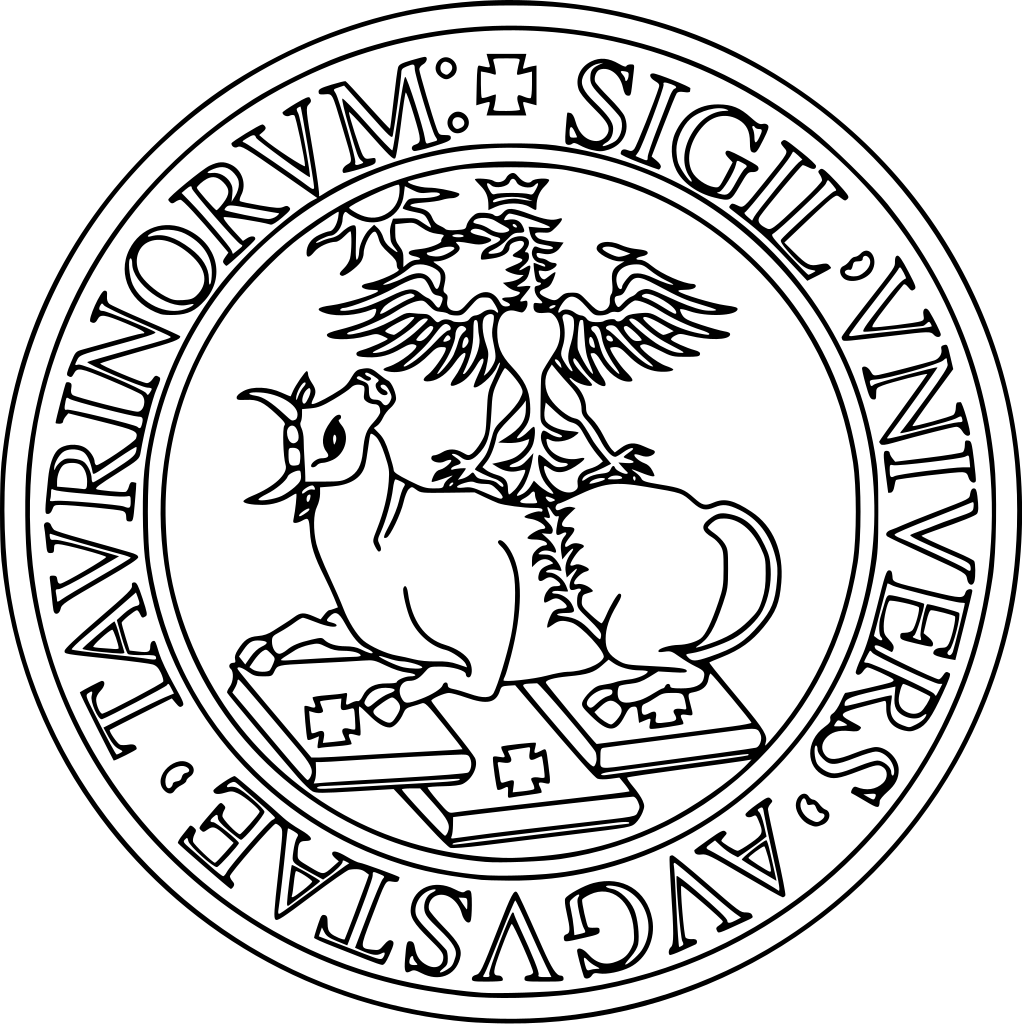
\includegraphics[width=0.25\linewidth]{images/Unito-logo}
	\end{center}
	
	\end{minipage}
	
	\vfill
	
	% Logo and other info
	% \begin{minipage}{0.8\textwidth}
	%    \centering
	%    \small
	
	% Examiner
	%    \begin{minipage}[t]{0.29\textwidth}
	%      \textsc{Titolari del corso} \\
	%     {\scriptsize Prof. Marco Costa\\
	%      Prof. Antonaldo Diaferio\\
	%       Università di Torino}
	%    \end{minipage}
	%   \hfill
	% Supervisor
	%   \begin{minipage}[t]{0.26\textwidth}
	%      \begin{center}
	%     	\textsc{Adattamento \LaTeX} \\ 
	%     \textsc{e integrazioni discutibili} \\
	%     {\scriptsize Massimo Bertolotti\\
	%      Università di Torino}
	%     \end{center}
	%   \end{minipage}
	%	\hfill
	%	\begin{minipage}[t]{0.27\textwidth}
	%	\raggedleft
	%	\textsc{Revisione contenutistica} \\ 
	%	{\scriptsize Elisa Antuca\\
	%	 Università di Torino}
	%	\end{minipage}
	%  \end{minipage}
	\end{center}
\end{comment}
\afterpage{\blankpage}
%% SVN info for this file
\svnidlong
{$HeadURL$}
{$LastChangedDate$}
{$LastChangedRevision$}
{$LastChangedBy$}

\begin{abstract}
  \noindent
  Nulla sed gravida lectus. Mauris blandit porttitor porta. Donec venenatis, sem
  ac ultricies aliquet, purus risus auctor erat, sit amet volutpat mauris sem
  feugiat orci. Integer vel dictum odio. Sed id nulla nunc, eget pretium
  neque. Duis sit amet consectetur leo. Cras nec nibh quam. Vestibulum ante
  ipsum primis in faucibus orci luctus et ultrices posuere cubilia Curae; Sed
  porta tempus ante in tempus. Ut at leo sed quam adipiscing laoreet. Sed sit
  amet dolor elit. Proin id justo et purus gravida viverra.

  Etiam eget dui ut nulla bibendum iaculis. Phasellus dapibus laoreet
  malesuada. Etiam risus nisi, interdum eu sodales vel, rhoncus in arcu. Sed
  eget eleifend libero. Etiam nec tristique nunc. Sed mollis lorem vel quam
  mattis a dictum mi pulvinar. Morbi ultricies vulputate lorem at luctus.

  Nunc pharetra, turpis nec semper varius, odio dui porta mi, vel rhoncus lacus
  tellus imperdiet ipsum. Nam tempor nisi porttitor lacus eleifend
  sodales. Donec velit urna, molestie ut sodales id, ultrices a ante. Donec
  bibendum eros vitae est suscipit ornare. Cras arcu felis, imperdiet vel
  laoreet eget, volutpat a nibh. Fusce vel justo eu libero ultricies molestie
  vel sed massa. Phasellus tincidunt elementum eros, eu elementum orci rhoncus
  nec. Donec vitae viverra mi. Sed quis iaculis sapien.

  Cras molestie, tortor a congue ultrices, lectus metus viverra massa, eu
  lacinia libero mauris nec est. Vestibulum a leo justo. Sed ac mauris nibh,
  eget fringilla enim. Mauris accumsan dapibus lorem quis blandit. Class aptent
  taciti sociosqu ad litora torquent per conubia nostra, per inceptos
  himenaeos. Vivamus tristique pharetra sem, sit amet rhoncus elit rhoncus
  id. Mauris fermentum risus egestas purus vehicula placerat. In hac habitasse
  platea dictumst. Etiam porttitor neque viverra metus sagittis euismod. Morbi
  nec euismod quam. Curabitur non justo sit amet quam gravida rhoncus nec a
  justo. Donec in tortor turpis. In porttitor facilisis mauris, vitae pretium
  dolor venenatis eget. Aenean sagittis, nisi eget euismod pulvinar, tortor
  sapien euismod ligula, id sollicitudin dolor ipsum eu eros. Nam scelerisque
  pretium ligula, eu fermentum erat dictum quis.
\end{abstract}

% SVN info for this file
\svnidlong
{$HeadURL$}
{$LastChangedDate$}
{$LastChangedRevision$}
{$LastChangedBy$}

\tableofcontents

\mainmatter

\part{Topologia generale}
\labelPart{first}
% SVN info for this file
\svnidlong
{$HeadURL$}
{$LastChangedDate$}
{$LastChangedRevision$}
{$LastChangedBy$}

\chapter{Spazi topologici}
\labelChapter{spazitopologici}

\begin{introduction}
‘‘BEEP BOOP INSERIRE CITAZIONE QUA BEEP BOOP.''
\begin{flushright}
	\textsc{NON UN ROBOT,} UN UMANO IN CARNE ED OSSA BEEP BOOP.
\end{flushright}
\end{introduction}


%\begin{introduction}
%  Tisca.
%\end{introduction}
\section{Spazio topologico}
\begin{define}
Uno \textbf{spazio topologico}\index{spazio topologico} $\left(X, \topo\right)$ è un insieme $X$ con una famiglia di sottoinsiemi $\topo\subseteq\setpart{X}$ detta \textbf{topologia}\index{topologia} che soddisfano i seguenti assiomi (detti \textbf{assiomi degli aperti}\index{assiomi!degli aperti}):
\begin{enumerate}
\item \textit{Il vuoto e l'insieme stesso sono aperti della topologia}: $\emptyset,\ X\in\topo$ .
\item \textit{L'unione arbitraria di aperti è un aperto}: dati $\left\{A_i\right\}_{i\in I}$ tale che $A_i\in\topo$ $\forall i\in I$ ($|I|\leq \infty$), allora $\displaystyle\union_{i\in I}A_i=A\in\topo$ .
\item \textit{L'intersezione finita di aperti è aperta}: sati $\left\{A_i\right\}_{i\in I}$ tale che $A_i\in\topo$ $\forall i\in I$ ($|I|< \infty$), allora $\displaystyle\inter_{i\in I}A_i=A\in\topo$.
\end{enumerate}
Gli elementi di $\topo$ si dicono \textbf{aperti}\index{aperto} della topologia.
\end{define}
\begin{define} Si può definire equivalentemente su X una topologia $\topo$ usando gli \textbf{assiomi dei chiusi}\index{assiomi!dei chiusi}):
\begin{enumerate}
	\item \textit{Il vuoto e l'insieme stesso sono chiusi della topologia}: $\emptyset,\ X\in\topo$.
	\item \textit{L'unione finita di chiusi è un chiuso}: dati $\left\{C_i\right\}_{i\in I}$ tale che $C_i\in\topo$ $\forall i\in I$ ($|I|< \infty$), allora $\displaystyle\union_{i\in I}C_i=C\in\topo$ .
	\item \textit{L'intersezione arbitraria di chiusi è un chiuso}: dati $\left\{C_i\right\}_{i\in I}$ tale che $C_i\in\topo$ $\forall i\in I$ ($|I|\leq \infty$), allora $\displaystyle\inter_{i\in I}C_i=C\in\topo$.
\end{enumerate}
Gli elementi di $\topo$ si dicono \textbf{chiusi}\index{chiuso} della topologia.
\end{define}
\begin{observe}
Per verificare il terzo assioma degli aperti (o, equivalentemente, il secondo dei chiusi) è sufficiente verificare che sia vero per soli due sottoinsiemi qualunque.
\end{observe}
\begin{example}~{}
\begin{itemize}
\item \textbf{Topologia discreta}\index{topologia!discreta}: $\topo=\setpart{X}$, \textit{tutti} gli insiemi sono \textit{aperti}.
\item \textbf{Topologia banale}\index{topologia!banale}: $\topo={\emptyset,\ X}$, \textit{tutti} gli insiemi sono \textit{aperti}.
\end{itemize}
\end{example}
\section{Distanza e spazi metrici}
\begin{define}
Su un insieme $X$ una funzione $\funz{d}{X\times X}{\realset}$ è una \textbf{distanza}\index{distanza} se:
\begin{enumerate}
\item \textit{Positività della distanza}: $\forall x,\ y\in X\quad \mvf{d}{x}{y}\geq 0$ e $\mvf{d}{x}{y}=0\iff x=y$
\item \textit{Simmetria}: $\forall x,\ y\in X\quad \mvf{d}{x}{y}=\mvf{d}{y}{x}$
\item \textbf{Disuguaglianza triangolare}\index{disuguaglianza triangolare}: $\forall x,\ y,\ z\in X\quad \mvf{d}{x}{z}\leq\mvf{d}{x}{y}+\mvf{d}{y}{z}$
\end{enumerate}
\end{define}
\begin{define}
Uno \textbf{spazio metrico}\index{spazio!metrico} $\left(X, d\right)$ è un insieme su cui è definita una distanza.
\end{define}
\begin{define}
Definita la \textbf{palla aperta di centro}\index{palla aperta} $x$ come l'insieme degli elementi di $X$ che soddisfano la seguente condizione:
\begin{equation}
B_{\epsilon}\left(x\right)=\left\{y\in X\mid \mvf{d}{x}{y}<\epsilon\right\}
\end{equation}
Ogni spazio metrico ha una \textbf{topologia} $\topo_d$ \textbf{indotta dalla distanza}, i cui aperti sono definiti come:
\begin{equation*}
A\subseteq X \text{ aperto } \left(A\in\topo\right) \text{ se } \forall x\in A\ \exists \epsilon>0\ \colon B_{\epsilon}\left(x\right)\subseteq A.
\end{equation*}
\end{define}
\begin{example}~{}
\begin{itemize}
\item Su un qualunque insieme $X$ si può definire la \textit{distanza banale}:
\begin{equation}
\mvf{d}{x}{y}=\begin{cases} 
	0 & \text{se }x=y\\
	1 & \text{se }x\neq y
\end{cases}
\end{equation}
In questo modo, ogni punto è una palla aperta e dunque ogni sottoinsieme è un aperto, dando allo spazio la \textit{topologia discreta}. In particolare, ogni insieme può essere uno spazio metrico.
\item Su $X=\realset$ si può definire come distanza il \textit{valore assoluto} $\mvf{d}{x}{y}=|x-y|$, che induce la \textbf{topologia Euclidea}\index{topologia!Euclidea} $\mathcal{E_{ucl}}$, definita con le palle aperte di raggio $\epsilon$:
\begin{equation}
	B_{\epsilon}\left(x\right)=\left\{y\in \realset\mid |x-y|<\epsilon\right\}
\end{equation}
nel seguente modo:
\begin{equation*}
A\subseteq \realset \text{ aperto } \left(A\in\mathcal{E_{ucl}}\right) \text{ se } \forall x\in A\ \exists \epsilon>0\ \colon B_{\epsilon}\left(x\right)\subseteq A.
\end{equation*}
\item Su $X=\realset^n$ si può definire come distanza la \textit{norma Euclidea}: $\mvf{d}{x}{y}=||x-y||$. che induce la \textit{topologia Euclidea} $\mathcal{E_{ucl}}$ in modo analogo al caso precedente.
\begin{gather*}
	B_{\epsilon}\left(x\right)=\left\{y\in \realset^n\mid ||x-y||<\epsilon\right\}\\
	A\subseteq \realset^n \text{ aperto } \left(A\in\mathcal{E_{ucl}}\right) \text{ se } \forall x\in A\ \exists \epsilon>0\ \colon B_{\epsilon}\left(x\right)\subseteq A.
\end{gather*}
\end{itemize}
\end{example}
\begin{attention}
Non tutte le topologie sono indotte da una distanza! Definiamo la \textbf{topologia dei complementari finiti} sull'insieme $X$ nel modo seguente:
\begin{gather*}
A\subseteq \realset \text{ aperto } \left(A\in CF\right) \text{ se } \forall X\setminus A \text{ è finito.}\\
C\subseteq \realset \text{ chiuso } \left(C\in CF\right) \text{ se } \forall C \text{ è finito.}
\end{gather*}
Alcune osservazioni:
\begin{itemize}
\item Se un aperto $A$ è tale se il suo complementare $\mathcal{C}A$ è finito, si ha che:
\begin{equation}
A=\mathcal{C}\left(\mathcal{C}A\right)=X\setminus\left(X\setminus A\right)=X\setminus\left\{\text{un numero finito di punti}\right\}
\end{equation}
In altre parole $A$ è aperto è pari ad $X$ privato al più di un numero finito di punti.
\item Se $X$ è finito, la topologia $CF$ coincide con la topologia discreta: ogni sottoinsieme di $X$ è finito e dunque un aperto.
\item Se $X$ è infinito, ad esempio $\realset$, la topologia \textit{non} è quella discreta: $[0,\ 1]$ per la topologia discreta è un chiuso ma per quella $CF$ non lo è in quanto \textit{non} è finito.
\end{itemize}
\end{attention}
\subsection{Norme esotiche}
Possiamo definire su $\realset^n$ una famiglia di distanze dette \textbf{norme}\index{norma}; qui di seguito ne elenchiamo alcune. Definiti i punti $x=\left(x_1,\ldots, x_n\right),\ y=\left(y_1,\ldots, y_n\right)\in\realset^n$ abbiamo:
\begin{itemize}
\item \textbf{Norma infinito}: $\displaystyle\mvf{d_\infty}{x}{y}=\max_{i}{|x_i-y_i|}$
\item \textbf{Norma uno}: $\displaystyle\mvf{d_1}{x}{y}=\sum_{i=1}^{n}|x_i-y_i|$
\item \textbf{Norma due}: $\displaystyle\mvf{d_2}{x}{y}=\sqrt{\sum_{i=1}^{n}|x_i-y_i|^2}$
\item \textbf{Norma p}: $\displaystyle\mvf{d_p}{x}{y}=\sqrt[\leftroot{1}\uproot{3}p]{\sum_{i=1}^{n}|x_i-y_i|^p}$
\end{itemize}
Si ha inoltre $\displaystyle \lim_{p \to +\infty}d_p=d_\infty$.\\
Valgono inoltre le seguenti disuguaglianze:
\begin{equation}
\forall x,\ y\in\realset^n\quad \mvf{d_\infty}{x}{y}\leq\mvf{d_2}{x}{y}\leq\mvf{d_1}{x}{y}\leq n\mvf{d_\infty}{x}{y}
\end{equation}
\begin{demonstration}
Supponiamo senza perdere di generalità che $\mvf{d_\infty}{x}{y}=|x_1-y_1|$.
\begin{gather*}
\mvf{d_2}{x}{y}=\sqrt{|x_1-y_1|^2+\ldots+|x_n-y_n|^2}\geq\sqrt{|x_1-y_1|^2}=|x_1-y_1|=\mvf{d_\infty}{x}{y}\\
\mvf{d_2}{x}{y}=|x_1-y_1|+\ldots+|x_n-y_n|\leq|x_1-y_1|+\ldots+|x_1-y_1|=n|x_1-y_1|=n\mvf{d_\infty}{x}{y}
\end{gather*}
Notiamo che $|x_i-y_i|$ sono sempre positive, allora sia $a_i\coloneqq|x_i-y_i|$. Segue che $a_1^2+\ldots+a_n^2\leq (a_1+\ldots+a_n)^2$ perché $a_i,\ldots,a_n\geq0$. Allora:
\begin{equation*}
\sqrt{a_1^2+\ldots+a_n^2}\leq a_1+\ldots+a_n\implies d_2\leq d_1
\end{equation*}
\end{demonstration}
Queste disuguaglianze danno le seguenti inclusioni\footnote{Qui usiamo la notazione $B_i\left(r\right)$ per indicare la palla aperta di raggio $r$ e centro fissato $x$ rispetto alla norma $i$.}:
\begin{equation}
B_1\left(\epsilon\right)\subseteq B_2\left(\epsilon\right)\subseteq B_\infty\left(\epsilon\right)\subseteq B_1\left(n\epsilon\right)
\end{equation}
\begin{center}
	\hspace*{-12cm}\begin{minipage}{.2\linewidth}
		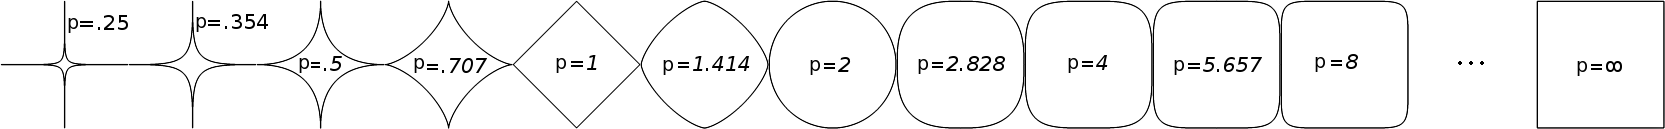
\includegraphics[trim=18.1cm 0cm 0cm 0cm,clip,scale=0.37]{images/pnorm.png}
	\end{minipage}
\end{center}
Questo ci porta a dire che le topologie indotte da queste distanze sono la stessa.\\
Preso adesso $X=\mathcal{C}\left([0,\ 1]\right)=\left\{\funz{f}{[0,\ 1]}{\realset},\ f\text{ continua}\right\}$, esso è uno spazio vettoriale infinito, con $0_\mathcal{C}\equiv O_{[0,\ 1]}$ (cioè la funzione \textit{identicamente nulla}). In questo caso possiamo comunque adattare le norme precedenti con delle ‘‘somme infinite'', ovvero degli integrali.
\begin{itemize}
	\item \textbf{Norma infinito}: $\displaystyle\mvf{d_\infty}{f}{g}=\max_{x\in[0,\ 1]}{|f(\left(x\right)-\left(y\right)|}$
	\item \textbf{Norma uno}: $\displaystyle\mvf{d_1}{f}{g}=\int_{0}^{1}|f(\left(x\right)-\left(y\right)|$
	\item \textbf{Norma due}: $\displaystyle\mvf{d_2}{f}{g}=\sqrt{\int_{0}^{1}|f(\left(x\right)-\left(y\right)|^2}$
	\item \textbf{Norma p}: $\displaystyle\mvf{d_p}{f}{g}=\sqrt[\leftroot{1}\uproot{3}p]{\int_{0}^{1}|f(\left(x\right)-\left(y\right)|^p}$
\end{itemize}
A differenza del caso su $\realset^n$, ogni norma genera in realtà una topologia distinta!
\section{Finezza: confronto di topologia}
\begin{define}\index{finezza}
Sia $X$ un insieme e $\topo_1$, $\topo_2$ due topologie di $X$. Si dice che $\topo_1$ è \textbf{meno fine}\index{finezza!meno fine} di $\topo_2$ se tutti gli aperti della prima topologia sono aperti della seconda:
\begin{equation}
\forall A\in\topo_1\implies A\in \topo_2
\end{equation}
In modo analogo si dice anche che $\topo_2$ è \textbf{più fine}\index{finezza!più fine} di $\topo_1$.
\end{define}
In altre parole, una topologia più fine ha più aperti rispetto a quella confrontata.
\begin{example}~{}
\begin{itemize}
\item La \textit{topologia banale} è la \textit{meno fine} di tutte, dato che ogni topologia contiene $\emptyset$, $X$.
\item La \textit{topologia discreta} è la \textit{più fine} di tutte, dato che ogni topologia è contenuta in $\setpart{X}$.
\item Su $\realset$ la topologia dei complementari finiti è \textit{meno fine} di quella euclidea. Infatti un aperto $A\in CF$ su $\realset$ è definito come $A=\realset\setminus\left\{x_1,\ldots,x_n\right\}$, cioè:
\begin{equation*}
A=\left(-\infty,\ x_1\right)\cup\left(x_1,\ x_2\right)\cup\ldots\cup\left(x_n,\ +\infty\right)
\end{equation*}
Per $n$ punti gli $n+1$ intervalli ottenuti sono aperti della topologia euclidea; essendo unione di aperti, anche $A$ è un aperto di $\mathcal{E_{ucl}}$
\end{itemize}
\end{example}
\begin{observe}\label{intersezionetopo}
	Se definiamo due topologie $\topo_1$ e $\topo_2$ sono due topologie di un insieme $X$, l'intersezione $\topo_1\cap\topo_2$ è anch'essa una topologia di $X$ e, per costruzione, è \textit{meno fine} di $\topo_1$ e $\topo_2$.
\end{observe}
\section{Base della topologia}
\begin{define}
Sia $\left(X, \topo\right)$ uno spazio topologico. $\basis$ è una \textbf{base}\index{base} per $\topo$ se:
\begin{enumerate}
\item \textit{La base è costituita da paerti per la topologia $\topo$}: $A\in\basis\implies A\in\topo (\basis\subseteq\topo)$.
\item \textit{Tutti gli aperti della topologia sono unioni degli aperti delle basi}:
$A\in\topo\implies\exists B_i\in\basis,\ i\in I\colon A=\union_{i\in I}B_i$.
\end{enumerate}
\end{define}
\begin{attention}
La base $\basis$ non è detto che sia una topologia! Ad esempio, le unioni sono aperti della topologia, ma non è detto che siano interni alla base $\basis$.
\end{attention}
\begin{example}~{}
\begin{itemize}
\item Nella \textit{topologia euclidea} di $\realset^n$ una base è
\begin{equation}
\basis=\left\{B_{\epsilon}\left(x\right)\mid x\in\realset^n,\ \epsilon>0\right\}
\end{equation}
Infatti, $\forall x\in A$ aperto $\exists\epsilon_x>0\ \colon B_{\epsilon_x}\left(x\right)\subseteq A$ per la definizione della topologia; segue che $A=\union_{x\in A}B_{\epsilon_x}\left(x\right)$.
\item Nella \textit{topologia euclidea} di $\realset$ una base è
\begin{equation}
	\basis=\left\{\left(a,\ b\right)\mid a,\ b\in \realset\right\}
\end{equation}
Un'altra base per $\realset$ nella $\mathcal{E_{ucl}}$ è 
\begin{equation*}
	\basis=\left\{\left(a,\ b\right)\mid a,\ b\in \rationalset\right\}
\end{equation*}
Dato $x\in\realset$, esiste sempre una successione $\left\{x_n\right\}\in\rationalset$ decrescente o crescente tale che $\displaystyle\lim_{n \to +\infty}x_n=x$, essendo $\rationalset$ denso in $\realset$\footnote{Per una discussione più approfondita a riguardo, si guardi sez. \textbf{XXX} a pag. \textbf{XXX}.}. Allora presa $a_n\searrow a$ e $b_n\nearrow b$, si ha:
\begin{equation*}
\left(a,\ b\right)=\union_{n\in \naturalset}\left(a_n,\ b_n\right)
\end{equation*}
Questa base con estremi razionali ha \textit{infiniti elementi}, ma in \textit{misura minore} rispetto a quella ad estremi reali.
\end{itemize}
\end{example}
\begin{theorema}\textsc{Teorema delle basi. (Manetti, 3.7)}\index{teorema!delle basi}\label{teoremabasi}\\
Sia $X$ un insieme e $\basis\subseteq\setpart{X}$ una famiglia di sottoinsiemi di $X$. $\basis$ è la base di un'\textit{unica} topologia \textit{se e solo se}:
\begin{enumerate}
\item \textit{L'insieme} $X$ \textit{deve essere scritto come unione di elementi della famiglia}: $\displaystyle X=\union_{B\in \basis}B$.
\item \textit{Per ogni punto dell'intersezione di elementi della famiglia deve esserci un'altro elemento di essa che contiene il punto ed è sottoinsieme dell'intersezione}:
\begin{equation}
	\forall A, B\in\basis\ \forall x\in A\cap B\ \exists C\in \basis\ \colon x\in C\subseteq A\cap B
\end{equation}
\end{enumerate}
\end{theorema}
\begin{demonstration}
Sia $\basis$ la famiglia di sottoinsiemi che verifica i punti $1$ e $2$. Allora devo trovare una topologia di cui $\basis$ è base. Definiamo $\topo$ tale che:
\begin{equation*}
A\in\topo\iff A\text{ è unione di elementi di }\basis
\end{equation*}
Verifichiamo gli assiomi degli aperti su $\topo$.
\begin{enumerate}[label=\Roman*]
\item $X\in\topo$ per ipotesi $1$, $\emptyset\in\topo$ perché è l'unione sugli insiemi di indici vuoto ($I=\emptyset$).
\item Sia $A_i=\union_{j}B_{ij}$, con $B_{ij}\in\basis$. Allora:
\begin{equation*}
\union_{i}A_i=\union_{i}\left(\union_{j}B_{ij}\right)=\union_{i,\ j}B_{ij}\implies\union_{i,\ j}A_i\in\topo
\end{equation*}
\item Sia $A, B\in\topo$, cioè $A=\union_{i}A_i$ e $B=\union_{j}B_j$ con $A_i, B_j\in\basis$. Allora:
\begin{equation*}
A\cap B=\left(\union_{i}A_i\right)\cap\left(\union_{j}B_j\right)=\union_{i,\ j}\left(\underbrace{A_i\cap B_j}_{\in\topo\text{ per l'ipotesi }2}\right)\in\topo%\qed
\end{equation*}
\end{enumerate}
\end{demonstration}
\begin{example}
Sia $X=\realset$ e $\basis=\left\{[a,\ b)\mid a,\ b\in\realset\right\}$. Verifichiamo che $\basis$ soddisfa il teorema appena enunciato.
\begin{enumerate}
\item $\displaystyle\realset=\union_{n\in \naturalset}\left[-n,\ n\right)$.
\item Preso $[a, b)\cap[c, d)$ si ha che esso è $\emptyset$ o è $[e, f)$, con $e=\max\left\{a,\ c\right\}$, $f=\min\left\{b,\ d\right\}$; in entrambi i casi l'intersezione è elemento di $\basis$.
\end{enumerate}
Esiste dunque una topologia su $\realset$ che ha base $\basis$; questa \textit{non} è base per la topologia Euclidea, ad esempio, dato che gli intervalli semiaperti non sono inclusi in $\mathcal{E_{ucl}}$.\\
Notiamo inoltre che $\displaystyle\left(a,\ b\right)=\union_{n\in \naturalset}\left[a+\frac{1}{n},\ b\right)$, dunque la topologia definita $\basis$ comprende gli aperti della topologia Euclidea: $\mathcal{E_{ucl}}$ è meno fine di questa topologia.
\end{example}
\section{Altri concetti topologici: chiusura, interno, frontiera e densità}
Ricordiamo che, dato uno spazio topologico $\left(X,\ \topo\right)$ e un sottoinsieme $A\subseteq X$, si ha:
\begin{itemize}
\item $A$ \textit{aperto} della topologia se $A\in\topo$.
\item $A$ \textit{chiuso} della topologia se $\mathcal{C}A=X\setminus A\in\topo$.
\end{itemize}
\begin{attention}
Essere aperto oppure essere chiuso \textit{non si escludono a vicenda}! Un insieme può essere aperto, chiuso, entrambi o nessuno dei due. Ad esempio, il vuoto e l'insieme stesso sono aperti e chiusi allo stesso tempo, dato che per ipotesi sono aperti i loro complementari $\mathcal{C}\emptyset = X\setminus \emptyset = X$ e $\mathcal{C}X = X\setminus X = \emptyset$ sono anch'essi aperti.
\end{attention}
\begin{define}
Sia $X$ spazio topologico e $A\subseteq X$. La \textbf{chiusura}\index{chiusura} $\overline{A}$ di $A$ è il più piccolo chiuso contente $A$:
\begin{equation}
\overline{A}=\inter_{\substack{A\subseteq C\\ C\text{ chiuso}}}C
\end{equation}
\textsc{Proprietà:}
\begin{itemize}
\item $A\subseteq \overline{A}$.
\item $\overline{A}$ è un chiuso in quanto intersezione (arbitraria) di chiusi.
\item $A$ è un chiuso $\iff A=\overline{A}$.
\end{itemize}
\end{define}
\begin{define}
Un punto $x$ è \textbf{aderente}\index{aderenza} ad $A$ se $x\in\overline{A}$.
\end{define}
\begin{define}
Sia $X$ spazio topologico e $A\subseteq X$. L'\textbf{interno}\index{interno} $\interior{A}$ di $A$ è il più grande aperto contenuto in $A$:
\begin{equation}
	\interior{A}=\union_{\substack{B\subseteq A\\ B\text{ aperto}}}B
\end{equation}
\textsc{Proprietà:}
\begin{itemize}
	\item $\interior{A}\subseteq A$.
	\item $\interior{A}$ è un aperto in quanto unione (arbitraria) di aperti.
	\item $A$ è un aperto $\iff A=\interior{A}$.
\end{itemize}
\end{define}
\begin{define}
	Un punto $x$ è \textbf{interno} ad $A$ se $x\in\interior{A}$.
\end{define}
\begin{define}
Sia $X$ spazio topologico e $A\subseteq X$. La \textbf{frontiera}\index{frontiera} $\partial A$ di $A$ sono i punti della chiusura di $A$ non contenuti nel suo interno o, in altri termini, i punti aderenti sia ad $A$ sia al suo complementare.
\begin{equation}
\partial A=\overline{A}\setminus \interior{A}=\overline{A}\cap\overline{X\setminus A}
\end{equation}
\textsc{Proprietà:}
\begin{itemize}
	\item $\partial{A}\subseteq \overline{A}$.
	\item $\partial{A}$ è un chiuso.
\end{itemize}
\end{define}
\begin{define}
Sia $X$ spazio topologico e $A\subseteq X$. A è \textbf{denso}\index{densità} è denso in $X$ se $\overline{A}=X$ o, in altri termini, tutti i punti di $X$ sono aderenti ad $A$.
\end{define}
\begin{example}
Il più piccolo chiuso contenente $\rationalset$ è $\realset$, poiché ogni reale è aderente ai razionali. Dunque $\rationalset$ è denso in $\realset$.
\end{example}
\section{Intorni}
\begin{define}
Sia $X$ spazio topologico e $x\in X$. $V$ è un \textbf{intorno}\index{intorno} di $x$ se $\exists A$ aperto tale che $x\in A\subseteq V$ o, in altri termini, se $x$ è interno ad $U$.
Definiamo inoltre la \textbf{famiglia degli intorni} di $x$ $I\left(x\right)\subseteq\setpart{X}$:
\begin{equation}
I\left(x\right)=\left\{V\subseteq X\mid V\text{ è intorno di }x \right\}
\end{equation}
\end{define}
\begin{observe}
	Dato $A\subseteq X$, per ogni $x\in A$ tale che $A$ è intorno di $x$ si può definire un aperto $A_x\subseteq A$, con $x\in A_x$. L'unione arbitraria di questi $A_x$ risulta essere contenuta in $A$ e pari al suo interno. Dunque, si può definire l'interno di $A$ come $\interior{A}=\left\{x\in A\mid A\in I\left(x\right)\right\}$; segue che $A$ è aperto se e solo se $A$ è intorno di ogni punto in $A$.
\end{observe}
\begin{lemming}\textsc{Proprietà degli intorni. (Manetti, 3.20, 3.21)}
\begin{enumerate}
\item \textit{Si possono estendere gli intorni}: $U\in I\left(x\right),\ U\subseteq V\implies V\in I\left(x\right)$
\item \textit{Le intersezioni di intorni sono ancora intorni}: $U,\ V\in I\left(x\right)\implies U\cap V\in I\left(x\right)$
\item \textit{Caratterizzazione della chiusura per intorni}:\\$B\subseteq X$, allora $x\in\overline{B}\iff\forall U\in I\left(x\right)\quad U\cap B\neq \emptyset$.
\end{enumerate}
\end{lemming}
\begin{demonstration}~{}
\begin{enumerate}[label=\Roman*]
\item L'aperto $A$ che soddisfa la definizione di $U\in I\left(x\right)$ è per costruzione contenuto anche in $V$, dunque $A$ è un aperto che soddisfa la definizione di $V$ intorno di $x$.
\item Definiti gli aperti $A_U\subseteq U,\ A_V\subseteq V$ che soddisfano la definizione di intorni di $x$, l'intersezione $A=A_U\cap A_V$ è un aperto contenente $x$. Dato che $A=A_U\cap A_V\subseteq U\cap V$, $U\cap V$ per definizione di intorno di $x$.
\item Per contronominale. \begin{align*}
	x\notin \overline{B} &\iff x\notin B \wedge x\notin \partial B\\
	&\iff x\in X\setminus B \wedge x\notin \overline{B}\cap\overline{X\setminus B}\\
	& \iff x\in X\setminus B \wedge x\notin \partial (X\setminus B)\\
	& \iff x\in \interior{\left(X\setminus B\right)}\\
	& \iff \exists U\in I\left(X\right)\ : x\in U\subseteq X\setminus B\\
	&\iff \exists U\in I\left(x\right)\ \colon U\cap B=\emptyset%\qed
\end{align*} 
\end{enumerate}
\end{demonstration}
\begin{define}
Sia $X$ spazio topologico, $x\in X$ e $I\left(x\right)$ la famiglia degli intorni di $x$. Una sottofamiglia $\mathcal{I}\subseteq I\left(x\right)$ è un \textbf{sistema fondamentale di intorni}\index{sistema fondamentale di intorni} di $x$ se $\forall U\in I\left(x\right)\exists V\in\mathcal{J}\ \colon V\subseteq U$.
\end{define}
%%% fine %%%
\section{Funzioni continue}
\begin{define}
Siano $X$, $Y$ spazi topologici. Una funzione $\funz{f}{X}{Y}$ si dice \textbf{continua}\index{continuità}\index{continuità!per aperti o chiusi}\seeonlyindex{funzione!continua}{continuità!per aperti o chiusi} se la controimmagine di aperti in $Y$ è un aperto in $X$:
\begin{equation}
\forall A\text{ aperto in } Y,\ f^{-1}\left(A\right) \text{ è aperto in } X
\end{equation}
Alternativamente, $f$ è continua se la controimmagine di chiusi in $Y$ è un chiuso in $Y$.
\begin{equation}
	\forall C\text{ chiuso in } Y,\ f^{-1}\left(C\right) \text{ è chiuso in } X
\end{equation}
\end{define}
\begin{observe}~{}
\begin{itemize}
\item Si ha la definizione di continuità con i chiusi perché la controimmagine si ‘‘comporta bene'' con i complementari:
\begin{equation*}
f^{-1}\left(Y\setminus A\right)=X\setminus f^{-1}\left(A\right)
\end{equation*}
\item È sufficiente verificare la definizione per gli aperti una base di $Y$ perché la controimmagine si ‘‘comporta bene'' con le unioni di insiemi:
\begin{equation*}
f^{-1}\left(\union_{i}A_i\right)=\union_{i}f^{-1}\left(A_i\right)
\end{equation*}
\end{itemize}
\end{observe}
\begin{lemming}\textsc{(Manetti, 3.25)}\\
Siano $X$, $Y$ spazi topologici e $\funz{f}{X}{Y}$ funzione.
$f$ è continua $iff$ $\forall A\subseteq X\quad f\left(\overline{A}\right)\subseteq\overline{f\left(A\right)}$.
\end{lemming}
\begin{demonstration}
Ricordiamo che per ogni funzione si ha:
\begin{itemize}
\item $f\left(f^{-1}\left(C\right)\right)\subseteq C$
\item $A\subseteq f^{-1}\left(f\left(A\right)\right)$
\end{itemize} 
$\impliesdx$ Sia $A\subseteq X$. Dobbiamo dimostrare che $f\left(\overline{A}\right)\overline{f\left(A\right)}$. Sappiamo che se un insieme è contenuto in un altro, lo stesso vale per le immagini e le controimmagini. Allora:
\begin{gather*}
f\left(A\right)\subseteq \overline{f\left(A\right)}\\
A\subseteq f^{-1}\left(f\left(A\right)\right)\subseteq f^{-1}\left(\overline{f\left(A\right)}\right)
\end{gather*}
$f^{-1}\left(\overline{f\left(A\right)}\right)$ è un chiuso (in $X$ in quanto controimmagine tramite una funzione continua di un chiuso) che contiene $A$.
Ma allora anche la chiusura, che è il più piccolo chiuso contenente $A$, è contenuta in $f^{-1}\left(\overline{f\left(A\right)}\right)$. Segue quindi:
\begin{gather*}
	\overline{A}\subseteq f^{-1}\left(\overline{f\left(A\right)}\right)\\
	f\left(\overline{A}\right)\subseteq f\left(f^{-1}\left(f\left(A\right)\right)\right)\subseteq\overline{f\left(A\right)}
\end{gather*}
$\impliessx$ Sia $C\subseteq Y$ chiuso e sia $A=f^{-1}\left(C\right)$. Dobbiamo dimostrare che $A$ è chiuso in $X$.
Poiché $A\subseteq \overline{A}$ è vero per definizione, dimostriamo che $\overline{A}\subseteq A$. Per ipotesi:
\[
\begin{gathered}[b]
f\left(\overline{A}\right)\subseteq\overline{f\left(A\right)}\\
f\left(\overline{f^{-1}\left(C\right)}\right)\subseteq\overline{f\left(f^{-1}\left(C\right)\right)}\subseteq \overline{C}=C
\end{gathered}
%\qed
\]
Applicando nuovamente la controimmagine:
\begin{gather*}
f\left(\overline{f^{-1}\left(C\right)}\right)\subseteq C\\
\overline{A}=\overline{f^{-1}\left(C\right)}\subseteq f^{-1}\left(f\left(\overline{f^{-1}\left(C\right)}\right)\right)\subseteq f^{-1}\left(C\right)=A
\end{gather*}
Dunque la controimmagine $A$ di un chiuso $C$ è un chiuso.%\qed
\end{demonstration}
\begin{theorema}\textsc{Manetti, 3.26}
La composizione di funzioni continue è continua.
\begin{equation}
\funz{f}{Y}{Z},\ \funz{g}{X}{Y}\text{ continue}\implies \funz{f\circ g}{X}{Z}\text{ continua}
\end{equation}
\end{theorema}
\begin{demonstration}
La controimmagine della composizione di funzioni $f\circ g$ è definita come $f^{-1}\left(f\circ g\right)=g^{-1}\circ f^{-1}$. Allora $A$ aperto in $Z\implies f^{-1}\left(A\right)$ aperto $\implies g^{-1}\left(f^{-1}\left(A\right)\right)$ aperto.%\qed
\end{demonstration}
\begin{define}\textsc{(Manetti, 3.27)}\\
Siano $X$, $Y$ spazi topologici e $\funz{f}{X}{Y}$ funzione. Dato $x\in X$ $f$ è \textbf{continua}\index{continuità!per intorni} in $x$ se:
\begin{equation}
	\forall U\in I\left(f\left(x\right)\right)\exists V\in I\left(x\right)\ \colon f\left(V\right)\subseteq U
\end{equation}
Questa è la generalizzazione della definizione tradizionale della continuità affrontata in \textit{Analisi UNO}.
\end{define}
\begin{theorema}\textsc{(Manetti, 3.28)}\\
Siano $X$, $Y$ spazi topologici e $\funz{f}{X}{Y}$ funzione. $f$ è continua per aperti $\iff$ $f$ è continua in $x\ \forall x\in X$.
\end{theorema}
\begin{demonstration}
$\impliesdx$ Sia $x\in X$ e $U\in I\left(f\left(x\right)\right)$. Per definizione di intorno $\exists A$ aperto in $Y$ tale che $f\left(x\right)\in A\subseteq U$.
Basta porre $V=f^{-1}\left(A\right)$: per continuità è aperto in $X$ e, dato che $x\in f^{-1}\left(A\right)$ perché $f\left(x\right)\in A$, allora $V$ è intorno di $x$. Segue che $f\left(V\right)=f\left(f^{-1}\left(A\right)\right)\subseteq A\subseteq U$.\\
$\impliessx$ Sia $A\subseteq Y$ aperto. Dobbiamo dimostrare che $f^{-1}\left(A\right)$ sia aperto. Preso $x\in f^{-1}\left(A\right)$ si ha che $f\left(x\right)\in A$; dunque $A$ è, in quanto aperto, intorno di $f\left(x\right)$. Allora, poiché $f$ è continua in $x$, $\exists V\in I\left(x\right)$ tale che $f\left(V\right)\subseteq A$.\\
Segue che $x\in V\subseteq f^{-1}\left(A\right)$, cioè $f^{-1}\left(A\right)$ è intorno di $x$ poiché contiene un intorno $V$ dello stesso punto. Dunque $f^{-1}\left(A\right)$ aperto perché è intorno di ogni suo punto.
\end{demonstration}
\begin{define}
Siano $X$, $Y$ spazi topologici e $\funz{f}{X}{Y}$ funzione.
\begin{itemize}
\item $f$ è \textbf{aperta}\index{funzione!aperta} se $\forall A$ aperto in $X$ $f\left(A\right)$ è aperto in $Y$.
\item $f$ è \textbf{chiusa}\index{funzione!chiusa} se $\forall C$ chiuso in $X$ $f\left(C\right)$ è chiuso in $Y$.
\end{itemize}
\end{define}
\begin{observe}
	È sufficiente verificare la definizione di funzione aperta per gli aperti di una base di $X$ perché l'immagine si ‘‘comporta bene'' con le unioni di insiemi:
	\begin{equation*}
		f\left(\union_{i}A_i\right)=\union_{i}f\left(A_i\right)
	\end{equation*}
\end{observe}
\begin{attention}
	Una funzione $f$ aperta che non sia omeomorfismo non è necessariamente una funzione aperta. Si prenda $\funztot{f}{\realset^2}{\realset}{\left(x,\ y\right)}{x}$ (la proiezione sulla prima coordinata):
	\begin{itemize}
		\item $f$ è \textit{continua} per ovvi motivi.
		\item $f$ è \textit{aperta}. Infatti, presa una base su $\realset^2$ come $\left\{B_{\epsilon}\left(x,\ y\right)\right\}$, si ha che $f\left(B_{\epsilon}\left(x,\ y\right)\right)=\left(x-\epsilon,\ x+\epsilon\right)$ che sono aperti in $\realset$.
		\item $f$ \textit{non} è \textit{chiusa}. Prendiamo $C=\left\{\left(x,\ y\right)\in \realset^2\mid xy=1 \right\}$ e definiamo la funzione $\funztot{g}{\realset^2}{\realset}{\left(x,\ y\right)}{xy}$ continua; vediamo facilmente come $C=g^{-1}\left(\left\{1\right\}\right)$ e, essendo ${1}$ chiuso in $\mathrm{R}$, $C$ è controimmagine continua di un chiuso e dunque chiuso.\\
		Si ha dunque $f\left(C\right)=\realset\setminus\left\{0\right\}$, che tuttavia non è un chiuso della topologia Euclidea in quanto non contiene infiniti punti (una base della $\mathcal{E_{ucl}}$ è formata da intervalli, che dunque contengono infiniti punti).
	\end{itemize}
\end{attention}
\begin{define}
Siano $X$, $Y$ spazi topologici e $\funz{f}{X}{Y}$ funzione. $f$ è un \textbf{omeomorfismo}\index{omeomorfismo} se è \textit{biunivoca}, \textit{continua} e la sua inversa è \textit{continua}; più precisamente, esiste $g\colon Y\rightarrow X$ continua tale per cui $g\circ f = Id_{X}$ e $f\circ g = Id_{Y}$.\\
Due spazi topologici si dicono \textbf{omeomorfi} se esiste un omeomorfismo fra i due; in notazione $X\cong Y$.
\end{define}
\begin{lemming}\textsc{(Manetti, 3.31)}\\
Siano $X$, $Y$ spazi topologici e $\funz{f}{X}{Y}$ funzione \textit{continua}. Allora vale:
\begin{enumerate}
\item $f$ omeomorfismo $\iff$ $f$ aperta e biettiva.
\item $f$ omeomorfismo $\iff$ $f$ chiusa e biettiva.
\end{enumerate}
\end{lemming}
\begin{demonstration}
Dimostriamo la prima condizione, la seconda è analoga.\\
$\impliesdx$ Un omeomorfismo è biettiva per definizione. Dimostriamo dunque che $f$ sia aperta, cioè $\forall A\in X$ aperto $f\left(A\right)\in Y$ è aperto. Ma definita $\funz{g}{Y}{X}$ l'inversa continua dell'omeomorfismo $f$ (cioè $f^{-1}=g$), si ha che $\forall A\in X$ $g^{-1}\left(A\right)=f\left(A\right)$ è aperto.\\
$\impliessx$ $f$ è già biettiva e continua per ipotesi. Dobbiamo dimostrare che l'inversa $\funz{g}{Y}{X}$ sia continua, cioè $\forall A\in X$ aperto $g^{-1}\left(A\right)\in Y$ è aperto. Ma $g^{-1}\left(A\right)=f\left(A\right)$ che è aperto perché $f$ è aperta.
\end{demonstration}
\section{Topologia indotta}\index{topologia!indotta}
\begin{define}
Dati:
\begin{itemize}
\item Uno spazio topologico $X$.
\item Un insieme $Y$.
\item Una funzione $\funz{f}{Y}{X}$
\end{itemize}
Allora su $Y$ si può definire la \textbf{topologia indotta} come la topologia meno fine tra tutte quelle che rendono $f$ continua.
\end{define}
\section{Sottospazio topologico}\index{sottospazio!topologico}
\begin{define}
Sia $X$ uno spazio topologico $\left(X,\ \topo\right)$ e $Y\subseteq X$ un suo sottoinsieme. Su $Y$ si può definire la seguente \textit{topologia di sottospazio}\index{topologia!di sottospazio}:
\begin{equation}
U\subseteq Y\text{ aperto in } Y \iff \exists V\subseteq X\text{ aperto in } X (V\in \topo)\ : U=V\cap Y
\end{equation}
Definita l'\textbf{inclusione}\index{inclusione} $\incltot{i}{Y}{X}{y}{y}$, la topologia di sottospazio è la topologia indotta da $i$, cioè la topologia meno fine fra tutte quelle che rendono continua l'inclusione.
\end{define}
\begin{demonstration}
Dimostriamo la continuità dell'inclusione. Se $A$ aperto in $X$, $i^{-1}\left(A\right)=A\cap Y$ (tutti gli elementi di $A$ contenuti in $Y$) è aperto in $Y$ per definizione.
\end{demonstration}
\begin{define}
	Sia $X$ uno spazio topologico $\left(X,\ \topo\right)$ e $Y\subseteq X$ un suo sottoinsieme. Allora:
	\begin{itemize}
		\item $A\subseteq Y$ \textbf{aperto} in $Y\iff A=U\cap Y$ con $U$ aperto in $X$.
		\item $C\subseteq Y$ \textbf{chiuso} in $Y\iff C=U\cap Y$ con $V$ chiuso in $X$.
		\item Se $\basis$ è una base della topologia di $X\implies \basis'\coloneqq\left\{B\cap Y\mid B\in\basis\right\}$ è base della topologia di sottospazio.
	\end{itemize}
\end{define}
\begin{observe}
	Se $A\subseteq Y$ è aperto della topologia di $X$, allora $A$ è aperto in $Y$ poiché $A=A\cap Y$.
\end{observe}
\begin{example} Sia $Y=\left[0,\ 1\right]\subset\realset=X$ in topologia Euclidea.
	\begin{itemize}
		\item $A=\left(\frac{1}{2},\ 1\right)$ è aperto in $Y$ in quanto è già aperto in $X$.
		\item $A=\left[\frac{1}{2},\ 1\right]$ è chiuso in $Y$ in quanto è già chiuso in $X$.
		\item $B=\left(\frac{1}{2},\ 1\right]$ è aperto in $Y$ in quanto si ha, ad esempio, $A=\left(\frac{1}{2},\ \frac{3}{2}\right)\cap Y$.
	\end{itemize}
\end{example}
\begin{lemming}\textsc{(Manetti, 3.55)}\\
Sia $A\subseteq Y\subseteq X$ con $X$ spazio topologico e $Y$ sottospazio topologico. Definiamo:
\begin{itemize}
\item $\mathcal{cl}_Y\left(A\right)=$ chiusura di $A$ in $Y$.
\item $\mathcal{cl}_X\left(A\right)=$ chiusura di $A$ in $X$.
\end{itemize}
Allora $\mathcal{cl}_Y\left(A\right)=c\mathcal{l}_X\left(A\right)\cap Y$.
\end{lemming}
\begin{demonstration}
Preso $\mathcal{C}=\left\{C\subseteq X\mid C\text{ chiuso in }X\text{ e } A\subseteq C\right\}$, per definizione di chiusura si ha:
\begin{equation*}
\mathcal{cl}_X\left(A\right)=\inter_{C\in\mathcal{C}}C
\end{equation*}
Ora sia $\mathcal{C}'=\left\{C\cap Y\mid C\in\mathcal{C}\right\}$. Allora, usando i chiusi del sottospazio:
\begin{equation*}
\mathcal{cl}_Y\left(A\right)=\inter_{C\in\mathcal{C}}\left(C\cap Y\right)=\left(\inter_{C\in\mathcal{C}}C\right)\cap Y=\mathcal{cl}_Y\left(A\right)
\end{equation*}.
\end{demonstration}
\subsection{Immersione}
\begin{define}
Sia $\funz{f}{X}{Y}$ funzione tra $X,\ Y$ spazi topologici. Se:\begin{itemize}
\item $f$ continua.
\item $f$ iniettiva
\end{itemize}
Allora $f$ è un'\textbf{immersione}\index{immersione} se e solo se ogni aperto in $X$ è controimmagine di un aperto di $Y$ per $f$, cioè se e solo se si ha che: 
\begin{equation}
B\subseteq X\text{ è aperto in }X\iff B=f^{-1}\left(A\right),\ A\text{ aperto in } Y
\end{equation}
\end{define}
\begin{observe}\label{omeomorfismoimmersione}
\item Per costruzione $f$ è immersione se la topologia su $X$ è la topologia indotta, dunque la meno fine che rende $f$ continua.
\item Se sull'immagine $f\left(X\right)\subseteq Y$ mettiamo la topologia di sottospazio di $Y$, si ha che
\begin{equation*}
\funz{f}{X}{Y}\text{ immersione}\iff \funz{f_{\bullet}}{X}{f\left(X\right)}\text{ è omeomorfismo}
\end{equation*}
\end{observe}
\begin{example} Esempio di \textit{non} immersione.
	\begin{equation}
		\substack{\left[0,\ 1\right)\rightarrow \realset^2\\t\mapsto \left(\cos 2\pi t,\ \sin 2\pi t\right)}
	\end{equation}
Notiamo innanzitutto che $f\left(\left[0,\ 1\right)\right)=S^{1}$. Si ha:
\begin{itemize}
\item $f_{\bullet}$ è continua per ovvi motivi
\item $f_{\bullet}$ iniettiva, dato che l'unico caso problematico poteva essere $t=1$ che \textit{non} nel dominio (si avrebbe avuto infatti $f_{\bullet}\left(0\right)=f_{\bullet}\left(1\right)$).
\item $f_{\bullet}$ suriettiva per costruzione.
\end{itemize}
Tuttavia $f_{\bullet}$ \textit{non} è immersione, dato che $f_{\bullet}^{-1}$ non è continua. Preso $P=\left(1,\ 0\right)\in S^1$, $f_{\bullet}^{-1}$ non è continua in $P$. Infatti, gli intorni di $0$ in $\left[0,\ 1\right)$ sono del tipo $U=[0,\ \epsilon)$, dunque dovrei trovare $\forall U$ un intorno $V$ di $P\in S^1\ \colon f_{\bullet}^{-1}\left(V\right)\subseteq U$.\\
Tuttavia, solo la parte superiore di $V\in I\left(P\right)$ ha la controimmagine interna ad $U$: la parte inferiore, poiché sono le immagini di punti prossimi all'estremo $1$ del dominio, non hanno controimmagini in $U$. Pertanto, non abbiamo l'omeomorfismo di $f_{\bullet}$ e dunque l'immersione.
\end{example}
\begin{define}
Sia $\funz{f}{X}{Y}$ funzione tra $X,\ Y$ spazi topologici.
\begin{itemize}
\item $f$ si dice \textbf{immersione aperta}\index{immersione!aperta} se $f$ è chiusa.
\item $f$ si dice \textbf{immersione chiusa}\index{immersione!chiusa} se $f$ è aperta.
\end{itemize}
\end{define}
\begin{lemming}\textsc{Manetti, 3.59}\\
Sia $\funz{f}{X}{Y}$ funzione \textit{continua} tra $X,\ Y$ spazi topologici.
\begin{enumerate}
\item $f$ iniettiva e aperta $\implies f$ è immersione (aperta)
\item $f$ iniettiva e chiusa $\implies f$ è immersione (chiusa)
\end{enumerate}
\end{lemming}
\begin{demonstration}
Dimostriamo il caso chiuso, il caso aperto è analogo.
Preso $C\subseteq X$ chiuso, sappiamo che $f\left(C\right)$ è chiuso in $Y$, ma possiamo sempre dire che $f\left(C\right)=f\left(C\right)\cap f\left(X\right)$ in quanto $f\left(C\right)\subseteq \cap f\left(X\right)$. Dunque $f\left(C\right)$ è un chiuso del sottospazio $f\left(X\right)$. Segue che ogni chiuso di $C$ è un chiuso dell'immagine di $f$, dunque $\funz{f_{\bullet}}{X}{f\left(X\right)}$ è:
\begin{itemize}
\item Continua perché lo è $f$.
\item Biunivoca perché $f_{\bullet}$ è iniettiva in quanto lo è $f$ e suriettiva per definizione.
\item Chiusa per costruzione.
\end{itemize}
$f_{\bullet}$ è dunque omeomorfismo ed $f$ è immersione (chiusa).
\end{demonstration}
\section{Prodotti topologici}
\begin{define}
Siano $P,\ Q$ spazi topologici e $P\times Q$ il suo prodotto cartesiano. Definite le \textbf{proiezioni}\index{proiezione}:
\begin{gather}
\funztot{p}{P\times Q}{P}{\left(x,\ y\right)}{x}\\
\funztot{q}{P\times Q}{Q}{\left(x,\ y\right)}{y}
\end{gather}
La \textbf{topologia prodotto}\index{topologia!prodotto} $\mathcal{P}$ è la topologia \textit{meno fine} fra quelli che rendono $p$ e $q$ \textit{continue}. In particolare, ricordando l'osservazione \ref{intersezionetopo}, la topologia prodotto è l'intersezione di \textit{tutte} le topologia che rendono continue $p$ e $q$.
\end{define}
\begin{theorema}\textsc{Manetti, 3.61}\label{topprodotto}
\begin{enumerate}
\item Una \textit{base} della topologia $\mathcal{P}$ è data dagli insiemi della forma $U\times V$ dove $U\subseteq P$ aperto, $V\subseteq Q$ aperto.
\item $p,\ q$ sono aperte; inoltre $\forall \left(x,\ y\right)\in P\times Q$ le restrizioni:
\begin{gather}
\funztot{p_{\mid}}{P\times \left\{y\right\}}{P}{\left(x,\ y\right)}{x}\\
\funztot{q_{\mid}}{\left\{x\right\}\times Q}{Q}{\left(x,\ y\right)}{y}
\end{gather}
Sono \textit{omeomorfismi}.\\
\item Data $\funz{f}{X}{P\times Q}$ con $X$ spazio topologico, si ha che:
\begin{equation}
f\text{ continua}\iff f_1=p\circ f,\ f_2=q\circ f\text{ continue}
\end{equation}
\end{enumerate}
\end{theorema}
\begin{demonstration}~{}
\begin{enumerate}[label=\Roman*]
\item Dimostriamo che:
\begin{enumerate}[label=\Alph*)]
\item La famiglia $\left\{U\times V\right\}$ è base per una topologia $\topo$.
\item $\mathrm{P}$ è meno fine di $\topo$.
\item $\topo$ è meno fine di $\mathrm{P}$.
\end{enumerate}
In questo modo avremo che la topologia $\topo$ è la topologia prodotto $\mathcal{P}$ e ne conosceremo una base.
\begin{enumerate}[label=\alph*)]
\item Segue dal teorema delle basi \ref{teoremabasi} (Manetti, 3.7). Infatti
\begin{enumerate}
\item $P\times Q$ appartiene alla famiglia $\left\{U\times V\right\}$, dato che per definizione gli insiemi stessi $P$ e $Q$ sono aperti.
\item L'intersezione di due elementi della famiglia appartiene alla famiglia:
$\left(U_1\times V_1\right)\cap\left(U_2\times V_2\right)=\left(U_1\cap U_2\right)\times \left(V_1\cap V_2\right)$.
\end{enumerate}
\item Per definizione $\mathcal{P}$ è la meno fine fra tutte le topologie sul prodotto. Dunque, per dimostrare A) basta vedere che $p,\ q$ sono continue rispetto alla topologia $\topo$.\\
Presa la proiezione $p$, sia $U\subseteq P$ aperto. Si ha che $p^{-1}\left(U\right)=U\times Q$ è aperto in $\topo$ in quanto è prodotto di aperti; in particolare sta nella base! Dunque $p$ è continua, e un ragionamento analogo vale per $q$.
\item Dobbiamo dimostrare che ogni aperto di $\topo$ è anche aperto di $\mathcal{P}$.\\
Presi $U\subseteq P$, $V\subseteq Q$ allora:
\begin{equation*}
U\times V=\left(U\cap P\right)\times\left(V\cap Q\right)=\left(U\times P\right)\cap \left(V\times Q\right)=p^{-1}\left(U\right)\cap q^{-1}\left(V\right)
\end{equation*}
Poichè $p,\ q$ sono continue e $U,\ V$ sono aperti, anche $p^{-1}\left(U\right),\ q^{-1}\left(V\right)$ sono aperti; segue che la loro intersezione è aperta e dunque $U\times V$ è aperto della topologia $\topo$.
\end{enumerate}
\item Dimostriamo il caso con $p_{\mid}$, dato che il caso con $q_{\mid}$ è analogo. Preso un aperto della base $U\times V$, studiamo gli aperti del sottospazio $P\times\left\{ y\right\}$.
\begin{equation*}
\left(U\times V\right)\cap \left(P\times\left\{ y\right\}\right)=\begin{cases}
\emptyset\qquad\text{ se }y\notin V\\
U\times\left\{y\right\}\qquad\text{ se }y\in V
\end{cases}
\end{equation*}
Gli aperti del sottospazio $P\times\left\{ y\right\}$ sono tutte e solo le unioni di $U\times\left\{ y\right\}$, al variare di $Y$ di aperti dello spazio $P$. Si ha dunque:
\begin{equation*}
p_{\mid}\left(U\times \left\{y\right\}\right)=U
\end{equation*}
Dunque, essendo $p_{\mid}$ continua perché restrizione della proiezione (che è continua per definizione), biettiva per costruzione e aperta per i risultati appena ottenuti si ha che $P\times\left\{ y\right\}$ e $P$ sono omeomorfi, cioè $p_{\mid}$ è omeomorfismo.\\
Per dimostrare che $p$ sia aperta, preso $A$ aperto in $P\times Q$, si ha:
\begin{equation}
p\left(A\right)=p\left[\union_{y\in\rationalset}\left(A\cap P\times\left\{ y\right\}\right)\right]=\union_{y\in\rationalset}p\left(A\cap P\times\left\{ y\right\}\right)
\end{equation}
Per i ragionamenti della prima parte, $A\cap P\times\left\{ y\right\}$ è aperto di $P\times\left\{ y\right\}$ e sappiamo dunque che $p_{\mid}\left(A\cap P\times\left\{ y\right\}\right)$ è aperto: ne segue che $p\left(A\cap P\times\left\{ y\right\}\right)$ è aperto in $P$ al variare di $y$. Allora anche $p\left(A\right)$ è aperto (in quanto è unione di aperti) e dunque $p$ è aperta.
\item $\impliesdx$ Poiché $\funz{f}{X}{P\times Q}$, $\funz{p}{P\times Q}{P}$ e $\funz{q}{P\times Q}{Q}$ sono continue, le composizioni $f_1=\funz{p\circ f}{X}{P}$, $f_2=\funz{q\circ f}{X}{Q}$ sono banalmente continue.
$\impliessx$ Dobbiamo dimostrare che $f$ sia continua. Sia $A=U\times V\subseteq P\times Q$ aperto della base:
\begin{align*}
f^{-1}\left(U\times V\right)=&f^{-1}\left(p^{-1}\left(U\right)\cap q^{-1}\left(V\right)\right)=f^{-1}\left(p^{-1}\left(U\right)\right)\cap f^{-1}\left(q^{-1}\left(V\right)\right) \\
=& \left(pf\right)^{-1}\left(U\right)\cap \left(qf\right)^{-1}\left(V\right)
\end{align*}
Per ipotesi $pf$, $qf$ sono continue, dunque loro controimmagini di aperti sono ancora aperti; inoltre, essendo la loro intersezione un aperto, segue l'implicazione.
\end{enumerate}
\end{demonstration}
\begin{proposition}
Siano $X,\ Y$ spazi topologici e $X\times Y$ il prodotto. Allora:
\begin{enumerate}
\item Date le basi $\basis$ della topologia di $X$ e $\mathcal{C}$ della topologia di $Y$, allora:
\begin{equation}
\mathcal{D}=\left\{U\times V\mid U\in\basis,\ V\in\mathcal{C}\right\}
\end{equation}
è una base per la topologia prodotto.
\item Dati $x\in X,\ y\in Y$, siano $\mathcal{U} = \left\{U_i\right\}_{i\in I}$ un
sistema fondamentale di intorni di $x$ e $\mathcal{V} = \left\{V_j\right\}_{j\in J}$ un sistema fondamentale di intorni di $y$. Poniamo $Wij \coloneqq U_i \times V_j \subseteq X \times Y$ . Allora:
\begin{equation}
\mathcal{W} = \left\{W_{ij}\right\}_{j\in J}
\end{equation}
è un sistema fondamentale di intorni di $\left(x,\ y\right) \in X \times Y$.
\item Se $A\subseteq X,\ B\subseteq Y$, allora $\overline{A\times B}=\overline{A}\times \overline{B}$. In particolare, il prodotto di chiusi è chiuso.
\end{enumerate}
\end{proposition}
\begin{demonstration}
\begin{enumerate}[label=\Roman*]
\item Segue dalla dimostrazione dal primo punto del teorema \ref{topprodotto} (\textsc{Manetti, 3.61}).
\item Per definizione di sistema fondamentale di intorni si ha:
\begin{gather*}
\forall U\in I\left(x\right)\ \exists U_i\in\mathcal{U}\ \colon U_i\in U\\
\forall V\in I\left(y\right)\ \exists V_i\in\mathcal{V}\ \colon V_j\in V\\
\end{gather*}
$\impliesdx$ Per ogni intorno $U$ di $x$ e $V$ di $y$, si ha $W\in I\left(x,\ y\right)$. Inoltre, presi gli intorni $U_i$ e $V_j$ definiti come sopra, si ha che $W_{ij} = U_i \times V_j\in I\left(x,\ y\right)$ per definizione di topologia prodotto; segue che, per ogni intorno $W$ di questa forma esiste $W_{ij}$ tale che:
\begin{equation*}
W_{ij} = U_i \times V_j\subseteq U\times V\subseteq W
\end{equation*}
$\impliessx$ Prendiamo un intorno $W\in I\left(x,\ y\right)$, esiste un aperto $W'\subseteq W$. Poiché $W'$ appartiene al prodotto $X\times Y$, si ha che $W'=\union_k U_k\times V_k$ con $U_k$ e $V_k$ aperti di $X$ e $Y$. Preso allora $\left(x,\ y\right)\in W'$, esiste gli aperti $U_k$ e $V_k$ che contengono rispettivamente $x$ e $y$.\\
Segue dunque che $U_k\in I\left(x\right)$ e $V_k\in I\left(y\right)$ e dunque dal sistema fondamentale di intorni si ha che $\exists U_i\in\mathcal{U},\ V_j\in\mathcal{V}$ tali che $U_i\in U_k,\  V_j\in V_k$. Allora definito $W_{ij} = U_i \times V_j$, si ha per ogni intorno $W$ di esiste $W_{ij}$ tale che:
\begin{equation*}
	W_{ij} = U_i \times V_j\subseteq U_k\times V_k\subseteq W'\subseteq W
\end{equation*}
\item \begin{align*}
\left(x\, y\right)\in \overline{A\times B}&\iff \forall W\in I\left(x,\ y\right)\quad W\cap\left(A\times B\right)\neq \emptyset\\
&\iff \forall U\in I\left(x\right),\ \forall V\in I\left(y\right)\quad \left(U\times V\right)\cap\left(A\times B\right)\neq \emptyset\\
&\iff \forall U\in I\left(x\right),\ \forall V\in I\left(y\right)\quad \left(U\cap A\right)\times\left(V\cap B\right)\neq \emptyset\\
&\iff \forall U\in I\left(x\right),\ \forall V\in I\left(y\right)\quad U\cap A\neq \emptyset ,\ V\cap B\neq \emptyset\\
&\iff \forall U\in I\left(x\right)\quad U\cap A\neq \emptyset ,\ \forall V\in I\left(y\right)\quad V\cap B\neq \emptyset\\
&\iff x\in\overline{A}\wedge y\in \overline{B}\iff\left(\right)\left(x\, y\right)\in\overline{A}\times \overline{B}
\end{align*}
In particolare, se $A$ e $B$ sono chiusi, avendo che $A=\overline{A}$ e $B=\overline{B}$, otteniamo:
\begin{equation*}
A\times B=\overline{A}\times \overline{B}=\overline{A\times B}
\end{equation*}
\end{enumerate}
\end{demonstration}
\begin{observe}
Il prodotto di un numero \textbf{finito} di spazi topologici è pari al prodotto di due spazi:
\begin{equation*}
X\times Y\times Z=\left(X\times Y\right)\times Z
\end{equation*}
In particolare una base di aperti di $X_1\times \ldots \times X_n$ è data da:
\begin{equation*}
\basis=\left\{A_1\times \ldots \times A_n\mid A_i\text{ aperto in } X_i\right\}
\end{equation*}
\end{observe}
\section{Assiomi di separazione: T1 e Hausdorff}\index{assioma di separazione}
\begin{define}
Uno spazio topologico $X$ si dice \textbf{T1}\index{assioma di separazione!T1}\index{spazio topologico!T1} se ogni sottoinsieme finito è chiuso, in particolare se e solo se tutti i punti sono chiusi.\\
In termini di intorni, $X$ è \textbf{T1} se presi due punti distinti $x$ e $y$ esiste un intorno per il punto $x$ che non contiene $y$ e viceversa:
\begin{equation}
\forall x,\ y\in X\quad x\neq y\implies
\begin{array}{l}
	\exists U\in I\left(x\right)\quad y\notin U\\
	\exists V\in I\left(y\right)\quad x\notin V
\end{array}
\end{equation}
\end{define}
\begin{demonstration} Dimostriamo che la definizione di \textbf{T1} implica quella per intorni e viceversa.\\
$\impliesdx$ Siano $x,\ y\in X\quad x\neq y$. Per ipotesi $\left\{x\right\}$ è chiuso, dunque $V=X\setminus\left\{x\right\}$ è aperto. Poiché $y\neq x$, allora $y\notin\left\{x\right\}\implies y\in V$, ed essendo $V$ aperto, $V\in I\left(y\right)$. Dunque $V$ è intorno di $y$ e banalmente $x\notin V$.\\
$\impliessx$ Dobbiamo dimostrare che $\forall x\quad \left\{x\right\}$ è chiuso, cioè $A=X\setminus\left\{x\right\}$ è aperto. Sia $y\in A$: $y\notin \left\{x\right\}\implies y\neq x$. Per ipotesi allora esiste un intorno $V$ di $y$ tale che $x\notin V$. Necessariamente si ha che $V\subseteq A$, dunque $A$ è anch'esso intorno di $y$. Per l'arbitrarietà di $y$, $A$ è intorno di ogni suo punto, dunque $A$ è aperto.
\end{demonstration}
\begin{observe}~{}
\begin{enumerate}
\item $X$ è \textbf{T1} se e solo se per ogni punto $x\in X$ si ha:
\begin{equation}
\left\{x\right\}=\inter_{U\in I\left(x\right)}U
\end{equation}
\item Ogni spazio metrico è \textbf{T1}
\end{enumerate}
\end{observe}
\begin{demonstration}
\begin{enumerate}[label=\Roman*]
\item $\impliesdx$ Se $X$ è \textbf{T1}, allora $\forall \left\{y\right\}\subseteq X$ è chiuso. Fissato $x$, prendiamo $y \in \inter_{U\in I\left(x\right)}U$. Allora $\forall U\in I\left(x\right)\ \left\{y\right\}\cap U\neq \emptyset$. Da ciò segue che $x\in\overline{\left\{y\right\}}=\left\{y\right\}$, cioè $y=x$. Allora $\left\{x\right\}=\inter_{U\in I\left(x\right)}U$.\\
$\impliessx$ Per dimostrare che $X$ è \textbf{T1} è sufficiente dimostrare che $\left\{x\right\}$ è chiuso, dato che ogni insieme finito in $X$ si può vedere come unione finita di singoletti $\left\{x\right\}$ e per gli assiomi dei chiusi otteniamo un chiuso. In particolare, ci basta dimostrare che $\overline{\left\{x\right\}}\subseteq \left\{x\right\}$, essendo l'altra implicazione ovvia per definizione.\\
Sia $y\in\overline{\left\{x\right\}}$. Per definizione di chiusura $\forall V\in I\left(y\right)\ V\cap\overline{\left\{x\right\}}\neq\emptyset\implies \forall V\in I\left(y\right)\ V\cap\overline{\left\{x\right\}}=\left\{x\right\}$, cioè l'intersezione dei $V$ deve incontrare $\left\{x\right\}$:
\begin{equation*}
\inter_{V\in I\left(y\right)}V\cap\left\{x\right\}=\left\{x\right\}
\end{equation*}
Per ipotesi, $\displaystyle \inter_{V\in I\left(y\right)}V=\left\{y\right\}$, dunque $\left\{y\right\}\cap \left\{x\right\}=\left\{x\right\}\implies y\in\left\{x\right\}\implies\overline{\left\{x\right\}}\subseteq \left\{x\right\}$ e vale le ipotesi.
\item Se $X$ è metrico e $x\in X$, il sistema fondamentale di intorni di $X$ sono gli intorni centrati in $X$ di raggio arbitrario, cioè $B_{\epsilon}\left(x\right)$. Allora:
\begin{equation*}
\inter_{U\in I\left(x\right)}U=\inter_{\epsilon > 0}B_{\epsilon}\left(x\right)=\left\{x\right\}
\end{equation*}
E per la proposizione precedente si ha che $X$ metrico è \textbf{T1}.
\end{enumerate}
\end{demonstration}
\begin{define}
Uno spazio topologico $X$ si dice di \textbf{Hausdorff}\index{assioma di separazione!Hausdorff}\index{spazio topologico!Hausdorff} o \textbf{T2}\seeonlyindex{spazio topologico!T2}{assioma di separazione!Hausdorff}\seeonlyindex{assioma di separazione!T2}{assioma di separazione!Hausdorff} se per ogni coppia di punti distinti esistono due intorni disgiunti:
\begin{equation}
	\forall x,\ y\in X\quad x\neq y\implies
	\begin{array}{l}
		\exists U\in I\left(x\right)\\
		\exists V\in I\left(y\right)
	\end{array}
\ \colon U\cap V=\emptyset
\end{equation}
\end{define}
\begin{observe}~{}
	\begin{enumerate}
		\item $X$ è di \textbf{Hausdorff} se e solo se per ogni punto $x\in X$ si ha:
		\begin{equation}
			\left\{x\right\}=\inter_{U\in I\left(x\right)}\overline{U}
		\end{equation}
	\item Essere \textbf{Hausdorff} implica essere \textbf{T1}, ma non il viceversa.
		\item Ogni spazio metrico è di \textbf{Hausdorff}. Infatti:
	\end{enumerate}
\end{observe}
\begin{demonstration}~{}
\begin{enumerate}[label=\Roman*]
\item $\impliesdx$ Sia $X$ di \textbf{Hausdorff}. Fissato $x$, sia $y\in\overline{U}$, con $U\in I\left(x\right)$. Per definizione di $\overline{U},\ \forall V\in I\left(y\right)\quad V\cap U\neq\emptyset$. Se $y \neq x$, si avrebbe un assurdo, dato che $\nexists V\in I\left(y\right)\ \colon U\cap V=\emptyset$ e dunque $X$ non sarebbe di \textbf{Hausdorff}.\\
$\impliessx$ Dobbiamo dimostrare che $X$ è di \textbf{Hausdorff}. Sia $x\neq y$. Allora $\displaystyle y\notin\left\{x\right\}=\inter_{U\in I\left(x\right)}\overline{U}$. Allora, per definizione di chiusura si ha che $\forall U\in I\left(x\right)\ \exists V\in I\left(y\right)\ \colon V\cap U=\emptyset$. Segue dunque la tesi.
\item Avendo per ogni coppia di punti distinti due intorni disgiunti in quanto \textbf{Hausdorff}, banalmente i due intorni verificano la definizione di \textbf{T1} per intorni.\\
Il viceversa \textit{non} è vero: prendendo la topologia dei complementari finiti $CF$ su uno spazio $X$ \textit{non} finito, essa è \textbf{T1} ma non \textbf{Hausdorff}.
\item Presi $x\neq y$, allora $\mvf{d}{x}{y}=d>0$. Dunque, per disuguaglianza triangolare si ha sempre che:
\begin{equation*}
B_{\nicefrac{d}{4}}\left(Y\right)\cap B_{\nicefrac{d}{4}}\left(Y\right)=\emptyset
\end{equation*}
\end{enumerate}
\end{demonstration}

rickrolled!
% SVN info for this file
\svnidlong
{$HeadURL$}
{$LastChangedDate$}
{$LastChangedRevision$}
{$LastChangedBy$}

\chapter{Connessione e compattezza}
\labelChapter{Connessocompatto}

\begin{introduction}
‘‘BEEP BOOP INSERIRE CITAZIONE QUA BEEP BOOP.''
\begin{flushright}
	\textsc{NON UN ROBOT,} UN UMANO IN CARNE ED OSSA BEEP BOOP.
\end{flushright}
\end{introduction}

\section{Connessione}
\begin{define}
Uno spazio topologico $X$ si dice \textbf{connesso}\index{connessione} se gli unici sottoinsiemi aperti e chiusi sono $\emptyset,\ X$.\\
Uno spazio non \textit{connesso} si dice \textbf{sconnesso} oppure \textbf{non connesso}.
\end{define}
\begin{lemming}\label{sconnesso}\textsc{(Manetti, 4.2)}\\
	Sono condizioni equivalenti:
	\begin{enumerate}
		\item $X$ è \textit{sconnesso}.
		\item $X=A\cup B$ con $A,\ B$ aperti, non vuoti, disgiunti
		\item $X=A\cup B$ con $A,\ B$ chiusi, non vuoti, disgiunti
	\end{enumerate}
\end{lemming}
\begin{demonstration}~{}\\
$2\iff3)$ Sono equivalenti: se $A$ è aperto e disgiunto da $B$ tale che $X=A\cup B$ significa che $B=\mathcal{C}A=X\setminus A$ e dunque chiuso; analogamente per $B$ aperto si ha che $A$ è chiuso: allora $A,\ B$ chiusi e aperti propri.\\
$1\implies2)$ Esiste $\emptyset\subsetneqq A \subsetneqq X$ con $A$ aperto e chiuso. Allora basta porre $B=\mathcal{C}A=X\setminus A$: essendo il complementare di $A$ è aperto e chiuso, sono disgiunti e tali per cui $B\neq X,\ B\neq \emptyset$. $A$ e $B$ soddisfano la tesi.\\
$1\implies2)$ $A$ aperto, $B$ aperto $\implies A$ chiuso perché $A=\mathcal{C}X=X\setminus B$. Inoltre $A$ non vuoto, $B$ non vuoto $\implies A\neq X$. Dunque $A$ è aperto, chiuso e $A\neq \emptyset,\ X$ e pertanto soddisfa la tesi: esiste un sottoinsieme aperto e chiuso che non il vuoto o l'insieme stesso.
\end{demonstration}
\begin{observe}
	Il lemma \ref{sconnesso} \textsc{(Manetti, 4.2)} ci dice che è sufficiente trovare solo due aperti (o chiusi) che soddisfano la condizione di cui sopra per affermare la sconnessione. Viceversa, per dimostrare la connessione, dobbiamo dimostrare che per ogni coppia di aperti (o chiusi) non vuoti, la cui unione è $X$, essi non siano disgiunti.
\end{observe}
\begin{example} Esempi di spazi topologici \textit{sconnessi} in topologia Euclidea.
	\begin{itemize}
		\item $X=\realset\setminus\left\{0\right\}=\left(-\infty,\ 0\right)\cup \left(0,\ +\infty\right)$
		\item $X=\left[0,\ 1\right]\cup \left(2,\ 3\right)$
	\end{itemize}
\end{example}
\begin{lemming}\textsc{(Manetti, 4.4)}\\
Sia $X$ spazio topologico e $A\subseteq X$ con $A$ aperto e chiuso. Sia $Y\subseteq X,\ Y$ \textit{connesso}. Allora $Y\cap A=\emptyset$ (cioè $Y\subseteq Y\setminus A$) oppure $Y\subseteq A$. 
\end{lemming}
\begin{demonstration}
Consideriamo $Y\cap A$: esso è intersezione di due aperti e chiusi per ipotesi ($Y$ è aperto e chiuso perché \textit{connesso}), cioè è aperto e chiuso. Essendo $Y$ \textit{connesso}, un suo sottoinsieme aperto e chiuso o è l'insieme vuoto oppure è l'insieme stesso, cioè $Y\cap A=\emptyset$ (cioè $Y\subseteq Y\setminus A$) oppure $Y\cap A=Y$ (cioè $Y\subseteq A)$.
\end{demonstration}
\begin{theorema}\textsc{(Manetti, 4.6)}\\
Con la topologia Euclidea, $X=\left[0,\ 1\right]$ è \textit{connesso}.
\end{theorema}
\begin{demonstration}
Supponiamo $X=\left[0,\ 1\right]=C\cup D$ con:
\begin{itemize}
	\item $C,\ D$ entrambi chiusi.
	\item $C,\ D$ entrambi aperti.
\end{itemize}
Dobbiamo dimostrare che $C,\ D$ \textit{non} sono disgiunti, ovvero $C\cap D\neq 0$. Supponiamo sia $0\in C$ e poniamo $d=\inf D$. Essendo $D$ un chiuso, $d\in \overline{D}=D$.
\begin{itemize}
	\item Se $d=0$, $d\in C\cap D\neq \emptyset$.
	\item Se $d>0$ allora $\left[0,\ d\right)\subseteq C$ perché \textit{non sta} in $D$. Il passaggio alla chiusura mantiene l'inclusione, dunque $\left[0,\ d\right]\subseteq \overline{C}=C$. Segue che $d\in C$ e dunque $C\cap D\neq \emptyset$.
\end{itemize}
\end{demonstration}
\begin{theorema}\textsc{(Manetti, 4.7)}\\
	L'immagine continua di un \textit{connesso} è un \textit{connesso}:
	\begin{equation}
		\funz{f}{X}{Y}\text{ continua},\ X\text{ connesso}\implies f\left(X\right)\text{ connesso}
	\end{equation}
\end{theorema}
\begin{theorema}
	Sia $Z\subseteq f\left(X\right)$, $Z$ aperto, chiuso in $f\left(X\right)$ non vuoto. Per dimostrare che $f\left(X\right)$ sia connesso ci è sufficiente dimostrare che $Z=f\left(X\right)$: in questo modo gli unici aperti e chiusi sono i sottoinsiemi impropri:
	\begin{itemize}
		\item $Z$ aperto: $\exists A$ aperto in $Y\ \colon Z=A\cap f\left(X\right)$.
		\item $Z$ chiuso: $\exists C$ chiuso in $Y\ \colon Z=C\cap f\left(X\right)$.
	\end{itemize}
Allora:
	\begin{itemize}
	\item $f^{-1}\left(Z\right)=f^{-1}\left(A\right)\cap f^{-1}\left(f\left(X\right)\right)=f^{-1}\left(A\right)\implies f^{-1}\left(Z\right)$ è uguale alla controimmagine continua di un aperto in $Y$, cioè è uguale ad un aperto di $X$.
	\item $f^{-1}\left(Z\right)=f^{-1}\left(C\right)\cap f^{-1}\left(f\left(X\right)\right)=f^{-1}\left(C\right)\implies f^{-1}\left(Z\right)$ è uguale alla controimmagine continua di un chiuso in $Y$, cioè è uguale ad un chiuso di $X$
	\end{itemize}
Segue che $f^{-1}\left(Z\right)$ è aperto e chiuso in $X$. Notiamo inoltre che, essendo $Z\neq \emptyset$, allora $f^{-1}\left(Z\right)\neq \emptyset$: essendo $X$ \textit{connesso} per ipotesi, necessariamente $f^{-1}\left(Z\right)=X$.
\end{theorema}
\begin{observe}
Dal teorema precedente segue che essere \textit{connesso} è una proprietà topologica! Infatti, se vale per una qualunque funzione continua $\funz{f}{X}{Y}$, allora varrà anche per omeomorfismi tra $X$ e $Y$; in particolare, si avrà per suriettività che $f\left(X\right)=Y$ connesso.
\end{observe}
\begin{define}
Un \textbf{arco}\seeonlyindex{arco}{cammino} o \textbf{cammino}\index{cammino} $\alpha$ da un punto $x$ a un punto $y$ in uno spazio topologico $X$ è una funzione continua che parametrizza un \textit{percorso} finito fra gli estremi $x$ e $y$:
\begin{equation}
\funz{\alpha}{\left[0,\ 1\right]}{X} \text{ continua}\ \colon \alpha\left(0\right)=x,\ \alpha\left(1\right)=y
\end{equation}
\end{define}
\begin{define}
Uno spazio topologico $X$ si dice \textbf{connesso per archi} o \textbf{c.p.a.}\index{connessione!per archi}\seeonlyindex{c.p.a.}{connessione!per archi} o \textit{path-connected} se per ogni coppia di punti in $X$ esiste un arco che li collega:
\begin{equation}
\forall x,\ y\in X\ \exists \funz{\alpha}{\left[0,\ 1\right]}{X} \text{ continua}\ \colon \alpha\left(0\right)=x,\ \alpha\left(1\right)=y
\end{equation}
\end{define}
\begin{theorema}\textsc{(Manetti, 4.7)}\\
$X$ \textbf{c.p.a.} $\implies X$ \textit{connesso}.
\end{theorema}
\begin{demonstration}
	Sia $X=A\cup B$, con $A,\ B$ aperti non vuoti. Vogliamo dimostrare che $A\cap B\neq \emptyset$. Essendo non vuoti, prendiamo $a\in A,\ b\in B$. In quanto $X$ è \textbf{c.p.a.}, esiste il cammino (continuo) $\funz{\alpha}{\left[0,\ 1\right]}{X}$ tale che $\alpha\left(a\right)=a,\ \alpha\left(1\right)=b$.\\
	Studiamo la controimmagine di $\alpha$:
	\begin{gather*}
		\alpha^{-1}\left(X\right)=\alpha^{-1}\left(A\cup B\right)=\left[0,\ 1\right]\\
		\left[0,\ 1\right]=\alpha^{-1}\left(A\cup B\right)=\alpha^{-1}\left(A\right)\cup \alpha^{-1}\left(B\right)
	\end{gather*}
$\alpha^{-1}\left(A\right),\ \alpha^{-1}\left(B\right)$ sono entrambi aperti e non vuoti in quanto controimmagini (continue) di aperti non vuoti ($0\in \alpha^{-1}\left(A\right),\ 1\in \alpha^{-1}\left(B\right)$).\\
Poiché $\left[0,\ 1\right]$ è connesso, allora le controimmagini trovate non sono disgiunte. Segue allora:
\begin{equation*}
\exists t\in \alpha^{-1}\left(A\right)\cap \alpha^{-1}\left(B\right)\implies \alpha\left(t\right)\alpha\left(\alpha^{-1}\left(A\right)\cap \alpha^{-1}\left(B\right)\right)\subset\alpha\left(\alpha^{-1}\left(A\right)\right)\cap\alpha\left(\alpha^{-1}\left(B\right)\right)=A\cap B
\end{equation*}
\end{demonstration}
\begin{define}
	Dati due cammini in uno spazio $X$:
	\begin{gather*}
		\funz{\alpha}{\left[0,\ 1\right]}{X}\quad \alpha\left(0\right)=x,\ \alpha\left(1\right)=y\\
		\funz{\beta}{\left[0,\ 1\right]}{X}\quad \beta\left(0\right)=y,\ \beta\left(1\right)=z\\	
	\end{gather*}
	Allora possiamo creare un cammino $\alpha \ast \beta$ con la \textbf{congiunzione di cammini}\index{cammino!congiunzione di cammini}:
	\begin{equation}
		\left(\alpha\ast\beta\right)\left(t\right)=\begin{cases}
			\alpha\left(2t\right)\quad\text{se }0\leq t\leq \frac{1}{2}\\
			\beta\left(2t-1\right)\quad\text{se }\frac{1}{2}\leq t\leq 1\\	
		\end{cases}
	\end{equation}
\end{define}
\begin{lemming}
	Sia $A,\ B$ \textbf{c.p.a}, $A\cap B\neq \emptyset\implies A\cup B$ \textbf{c.p.a.}
\end{lemming}
\begin{demonstration}
	Se $x, y\in A$ oppure $x,\ y\in B$ esiste per ipotesi un arco che li collega. Dobbiamo allora trovare un arco in $A\cup B$ da $x$ a $y$ $\forall x\in A, y\in B$. Preso $z\in A\cap B$, per ipotesi esistono due cammini ad esso:
	\begin{gather*}
		\funz{\alpha}{\left[0,\ 1\right]}{A}\quad \alpha\left(0\right)=x,\ \alpha\left(1\right)=z\\
		\funz{\beta}{\left[0,\ 1\right]}{B}\quad \beta\left(0\right)=z,\ \beta\left(1\right)=z\\	
	\end{gather*}
	Usando la \textit{giunzione di cammini}, si ha:
	\begin{equation}
		\left(\alpha\ast\beta\right)\left(t\right)=\begin{cases}
			\alpha\left(2t\right)\quad\text{se }0\leq t\leq \frac{1}{2}\\
			\beta\left(2t-1\right)\quad\text{se }\frac{1}{2}\leq t\leq 1\\	
		\end{cases}
	\end{equation}
	Il cammino $\funz{\alpha\ast\beta}{\left[0,\ 1\right]}{A\cup B}$ è quello richiesto.
\end{demonstration}
\begin{observe}~{}\label{giunzionecpa}
	\begin{itemize}
		\item Usando la giunzione di cammini, si ha che:
		\begin{equation*}
			X\text{ è \textbf{c.p.a.}}\iff \exists z\in X\ \colon \forall x\in X\quad
			\exists \funz{\alpha}{\left[0,\ 1\right]}{X}\ \colon \alpha\left(0\right)=z,\ \alpha\left(1\right)=x
		\end{equation*}
		In altre parole, uno spazio è \textbf{c.p.a.} se e solo se esiste un punto per cui ogni altro punto è collegato tramite un arco.
		\item Per ogni arco $\alpha$ esiste l'arco inverso, percorso al contrario: $\overline{\alpha}\left(t\right)=\alpha\left(1-t\right)$
	\end{itemize}
\end{observe}
\begin{define}
In $\realset^n$, un \textbf{segmento}\index{segmento} $\overline{PQ}$ è la combinazione lineare tra i punti $P$ e $Q$, parametrizzato come:
\begin{equation}
\overline{PQ}=\left\{P+tQ\mid t\in\left[0,\ 1\right]\right\}
\end{equation}
\end{define}
\begin{define}
	Un sottoinsieme $Y\subseteq\realset^n$ è \textbf{convesso}\index{convessità} se per ogni coppia di punti esiste un segmento che li collega contenuto interamente in $Y$.
	\begin{equation}
		\forall P,\ Q\in Y\quad \overline{PQ}\subseteq Y
	\end{equation}
\end{define}
\begin{define}
	Un sottoinsieme $Y\subseteq\realset^n$ è \textbf{stellato}\index{stellato} per $P$ se esiste un $P\in Y$ tale che per ogni altro punto esiste un segmento che li collega contenuto interamente in $Y$.
	\begin{equation}
		\exists P \in Y\ \colon \forall Q\in Y\quad \overline{PQ}\subseteq Y
	\end{equation}
\end{define}
\begin{example}~{}
\begin{itemize}
	\item Gli intervalli aperti e semiaperti sono \textbf{c.p.a}, dunque sono \textit{connessi}: l'arco $\alpha$ è banalmente il segmento pari all'intervallo aperto.
	\item Preso $X\subseteq\realset^n$ \textit{convesso}, qualunque segmento è anche per costruzione un arco: $X$ è anche \textbf{c.p.a} e dunque \textit{connesso}.
	\item $X=\realset^{2}\setminus\left\{0\right\}$ \textit{non} è \textit{convesso} (per $\left(0,\ 1\right)$ e $\left(0,\ -1\right)$ non si hanno segmenti interni ad $X$) ma è \textbf{c.p.a.} (basta prendere un cammino che ‘‘giri attorno'' all'origine) e dunque è \textit{connesso}.
	\item Preso $X\subseteq\realset^n$ \textit{stellato} per $P\in X$, qualunque segmento con $P$ è anche per costruzione un arco: $X$ è anche \textbf{c.p.a} per l'osservazione \ref{giunzionecpa} e dunque {connesso}.
	\item Ogni insieme \textit{convesso} è anche \textit{stellato} per $P$, basta fissare un qualunque punto come nostro $P$. In generale, un insieme è convesso se e solo se è stellato per ogni suo punto.
\end{itemize}
\end{example}
%RICKROLLED
Vediamo ora che conseguenze hanno questi teoremi in $\realset$ con la topologia euclidea.
\begin{theorema}
	Sia $I\subseteq \realset$ . Le seguenti affermazioni sono equivalenti:
		\begin{enumerate}
	\item $I$ è un intervallo, ovvero $I$ è convesso
	\item $I$ è c.p.a.
	\item $I$ è connesso			
		\end{enumerate}
\end{theorema}
\begin{demonstration}
	$1) \implies 2)$ Siccome $I$ è convesso $\Rightarrow$ $I$ stellato $\Rightarrow$ $I$ c.p.a. $\Rightarrow$ $I$ connesso. \\
	$2) \implies 3)$ Vale in generale che c.p.a. $\Rightarrow$ connesso.\\
	$3) \implies 1)$ Per contronominale mostriamo che $I$ non intervallo $\Rightarrow$ $I$ sconnesso. $I$ non intervallo significa che 
		\begin{gather*}
			\exists a<b<c,\ a,c\in I,\ b\notin I \\
			b\notin I \Rightarrow I= \left(\underbrace{ I\cap \left(-\infty ,b\right)}_{\in a}\ \right) \cup \left( \underbrace{I\cap \left(b ,+\infty\right)}_{\in c}\ \right)
		\end{gather*}
	ovvero $I$ è unione di aperti, non vuoti e disgiunti $\Rightarrow$ $I$ sconnesso.	
\end{demonstration}
\begin{observe}~{}\label{teorema esistenza zeri funzioni continue, s^n cpa}
		\begin{itemize}
	\item Come conseguenza immediata di questo teorema si ha il teorema di esistenza degli zeri per funzioni continue da $\realset$ in $\realset$, infatti se l'immagine continua di un connesso è un connesso, per tali funzioni vale che l'immagine continua di un intervallo è un intervallo.
	\item Per $n\geq 1$ la sfera $S^n := \left\{ \left(x_1,\dots,x_{n+1}\right) \mid \sum_{i=1}^{n+1}x_i^2=1 \right\}$ è c.p.a., infatti $\forall x,y\in S^n$ si trova sempre un arco come intersezione di $S^n$ e del piano $H$ passante per il centro della sfera, $x$ e $y$.
		\end{itemize}
\end{observe}

Vediamo ora un risultato per funzioni continue da $S^n$ in $\realset$
\begin{theorema}~{}\label{non iniettività S^n in realset}
	Sia $\funz f {S^n} \realset$ una funzione continua, Allora $\exists x\in S^n \ \colon f(x)=f(-x)$. In particolare $f$ non è iniettiva.
\end{theorema}
\begin{demonstration}
	Costruiamo una funzione $g(x)=f(x)-f(-x)$, essa è continua perché somma di funzioni continue. Siccome $S^n$ è connesso allora $g\left( S^n\right)\subseteq\realset$ è connesso $\Rightarrow$ per il teorema precedente $g\left(S^n\right)$ è un intervallo.\\
	Si considerino un punto $y\in S^n$ arbitrario e le sue immagini $g(y)$ e $g(-y)$: esse appartengono all'intervallo dell'immagine $g\left( S^n\right)$, quindi se ne può considerare il loro punto medio:
		\begin{gather*}
			\frac{1}{2}\left[ g(y) - g(-y)\right]=\frac{1}{2} \left[ f(y) -f(-y) - f(y) +f(-y) \right]= 0\\
			\Rightarrow \exists x\in S^n \colon g(x)=0, \text{ ovvero } f(x)=f(-x)
		\end{gather*}
\end{demonstration}


Come conseguenza di questo teorema si ha che un aperto di $\realset$ non sarà mai omeomorfo ad un aperto di $\realset^n$, vediamolo più precisamente.
\begin{theorema}
Sia $I\subseteq\realset$ e $U\subseteq\realset^n$, con $n\geq 2$. Se $I,U$ sono aperti allora $I$ non è omeomorfo a $U$.	
\end{theorema}	
\begin{demonstration}
	Si consideri un omeomorfismo $\funz g U I$. Siccome $U\subseteq\realset^n$ aperto allora esiste una palla aperta di raggio $\epsilon$ contenuta in $U$, se ne considera il bordo $S^n\subseteq U$. Si considera dunque la restrizione $\funz {g_{|_{S^n}}} {S^n} I$, che per il teorema precedente non è iniettiva. Dunque $g$ non è un omeomorfismo.	
\end{demonstration}

\begin{observe}
	Il teorema appena visto è un caso particolare del \textsc{teorema dell'invarianza della dimensione}, che cita: \newline
	Siano $U\subseteq\realset^n, V\subseteq\realset^m$ aperti. Se $U\cong V \Rightarrow n=m$. Equivalentemente $n\neq m\Rightarrow U\cancel\cong V$
\end{observe}

%LEZ 08
\begin{theorema}~{unione sottospazi connessi}
	Siano $\left\{ X_i \right\}_{i\in I}$ una famiglia di sottoinsiemi di uno spazio topologico $X$. Se ogni $X_i$ è connesso e $\inter_{i\in I}X_i\neq\emptyset$ allora $\union_{i\in I}X_i$ è connesso.	
\end{theorema}
\begin{demonstration}
	Sia $Z\subseteq Y:= \union_{i\in I}X_i$ un aperto, chiuso non vuoto. Vogliamo dimostrare che $Z=X$, cosicché $X$ risulti connesso. Basta l'inclusione $Y\subseteq Z$.\newline
	Si considera l'intersezione di $Z$ e di un connesso, dunque essa sarà banale
	\begin{gather*}
		X_i \cap Z = \begin{cases}
			\emptyset & \\
			X_i	&		
		\end{cases}
	\end{gather*}
	Dimostriamo ora che non è vuota, infatti siccome $Z$ non è vuoto ed è contenuto nell'unione ci sarà un connesso per cui l'intersezione non è vuota:
		\begin{gather*}
			Z\neq\emptyset, \ Z\subseteq \union_{i\in I}X_i \Rightarrow \exists i_0 \ \colon X_{i_0}\cap Z\neq \emptyset	\\
			\text{$X_{i_0}$ è connesso } \Rightarrow X_{i_0}\cap Z=X_{i_0} \Rightarrow X_{i_0}\subseteq Z \\
			\text{Siccome } \inter_{i\in I}X_i\neq\emptyset \Rightarrow \exists x\in\inter_{i\in I}X_i \Rightarrow x\in X_{i_0}\subseteq Z \Rightarrow x\in Z	\\
			\text{Siccome } x\in\inter_{i\in I}X_i$ e $x\in Z \Rightarrow \forall i\in I, \ X_i\cap Z\neq\emptyset
		\end{gather*}
	Quindi per $\forall i, \ X_i\subseteq Z \Rightarrow Y\subseteq Z \Rightarrow Y=Z$, quindi $Y$ è connesso perché l'unico aperto e chiuso non vuoto è banale ($Y$).
\end{demonstration}

\begin{theorema}~{}\label{prodotto connessi}
	$X, Y$ sono spazi topologici connessi $\iff X\times Y$ è connesso.	
\end{theorema}
\begin{demonstration}
	$\impliessx$ Si sfrutta la continuità delle proiezioni e che l'immagine continua di un connesos è connessa:
		\begin{gather*}
			\funz p {X\times Y} X \text{continua e suriettiva } \Rightarrow p(X)=X \text{ connesso} \\
			\funz q {X\times Y} Y \text{continua e suriettiva } \Rightarrow q(Y)=Y \text{ connesso}	
		\end{gather*}	
	$\impliesdx$ Si vuole sfruttare il teorema sull'unione di connessi, prestando attenzione che la loro intersezione non sia vuota, quindi si scrive il prodotto come unione di connessi già noti:
	$X\times Y=\union_{y\in Y}X\times\{y\}$, infatti $X\times\{y\}\cong X$ che per ipotesi è connesso , tuttavia $\inter_{y\in Y}X\times\{y\}=\emptyset$ !\newline
	Cerchiamo dunque di unire un insieme in modo tale che l'intersezione non sia vuota: sia $x_0\in X$ e $Y_{x_0}=\{x_0\}\times Y$ e poniamo $X_y=X\times\{y\}$ e si ha quanto voluto:
		\begin{gather*}
			X\times Y=\union_{y\in Y}X_y \cup Y_{x_0} \text{ e } X_y\cap Y_{x_0}=(x_0,y)\\
			\Rightarrow \inter_{y\in Y}\left( X_y  \cup Y_{x_0}\right)\neq\emptyset		
		\end{gather*}
	Dunque $X\times Y$ è unione di connessi la cui intersezione non è vuota, quindi per il teorema precedente è connesso.
%WELP COME CITO I TEOREMI%
\end{demonstration}

Approfondiamo ora la differenza fra essere spazio connesso o cpa mostrando esempi di un tipo ma non dell'altro. Prima però dimostreremo un teorema sulla caratterizzazione di un insieme denso che ci tornerà utile.
\begin{theorema}
	Sia $X$ uno spazio topologico e $A\subseteq X$ un suo sottoinsieme, allora
		\begin{gather*}
			A \text{ è denso }\iff \forall U\subseteq X \text{ aperto e } \ U\neq\epmtyset, \ \ U\cap A\neq\emptyset	
		\end{gather*}
\end{theorema}
\begin{demonstration}
	$\impliesdx$ Se $A$ è denso allora $\overline{A}=X$. Supponiamo che $\exists V$ aperto $\colon V\cap A=\emptyset$. Siccome $V$ è aperto allora $X\setminus V$ è chiuso, inoltre $V\cap A=\emptyset$, quindi $A\subseteq X\setminus V$. Essendo $A$ contenuto in un chiuso allora lo sarà anche la sua chiusura, siccome è il più piccolo chiuso che lo contiene:
		\begin{gather*}
			\overline{A}=X\subseteq X\setminus V \Rightarrow V=\emptyset
		\end{gather*}
	Ne segue che l'unico aperto che non interseca $A$ è l'insieme vuoto. \newline 
	$\impliessx$ Consideriamo un chiuso $K\supseteq A$. Siccome è chiuso allora il suo complementare $X\setminus K$ è aperto. Per ipotesi dunque si ha che $V\cap A\neq \emptyset$ oppure $V=\emptyset$, passando al complementare si ottiene che:
		\begin{gather*}
			A\subseteq K \Rightarrow X\setminus K \subseteq X\setminus A \Rightarrow V\subseteq X\setminus A \Rightarrow V\cap A=\emptyset \Rightarrow V=\emptyset \Rightarrow K=X \Rightarrow \overline{A}=X
		\end{gather*}
	L'ultima implicazione è dovuta al fatto che ogni chiuso che contiene $A$ si è dimostrato essere solo $X$ per cui esso sarà la sua chiusura.
\end{demonstration}

\begin{theorema}
	Sia $X$ uno spazio toplogico e $Y\subseteq X$ connesso, allora 
		\begin{equation*}
			\forall W \colon Y\subseteq W \subseteq \overline{Y} \Rightarrow W \text{ connesso}
		\end{equation*}
	In particolare la chiusura di un connesso è connessa.
\end{theorema}
\begin{demonstration}
	Per dimostrare che $W$ è connesso si considera un suo sottinsieme $Z\subseteq W$ aperto, chiuso e non vuoto e si mostra che è pari a $W$
		\begin{gather*}
			Z\subseteq W \text{ aperto } \Rightarrow \esists A\subseteq X \text{ aperto } \colon Z=W\cap A \\
			Z\subseteq W \text{ chiuso } \Rightarrow \esists C\subseteq X \text{ chiuso } \colon Z=W\cap C
		\end{gather*}
	Si vuole sfruttare il fatto che $Y$ è connesso:
		\begin{gather*}
			Z\cap Y=A\cap W\cap Y \stackrel{!}{=} A\cap Y \text{ aperto in Y}
			Z\cap Y=C\cap W\cap Y \stackrel{!}{=} C\cap Y \text{ aperto in Y}			
		\end{gather*}
	dove il passaggio indicato con (!) è dovuto al fatto che $Y\subseteq W$. Per poter sfruttare la connessione di $Y$ e dedurre che $Z\cap Y=Y$ dobbiamo prima provare che tale intersezione non è vuota e per farlo sfruttiamo il teorema precedente:
		\begin{gather*}
			Y \text{ denso in W, infatti  } \mathcal{cl}_W(Y)=\mathcal{cl}_X(Y)\cap W=\overline{Y}\cap W=W\\
			Z \text{ aperto in } W \Rightarrow Z\cap Y \neq \emptyset \Rightarrow Z\cap Y=Y \Rightarrow Y\subseteq Z
		\end{gather*}
	Tuttavia $Y$ è denso in $W$ e $Z$ è chiuso in $W$ che contiene $Y$, quindi 
		\begin{equation*}
			\mathcal{cl}_W(Y)=W\subseteq Z \Rightarrow W=Z \Rightarrow W \text{ connesso}
		\end{equation*}
\end{demonstration}

Vediamo ora degli esempi di spazi connessi ma non c.p.a.
\begin{example}~{seno del topologo}
	Sia $Y\subseteq \realset^2$ con la topologia euclidea e $Y=\left\{ \left( x, \frac{1}{x} \right) \mid x>0 \right\}$, detto anche seno del topologo. Esso è c.p.a. perché per connettere due punti basta percorrere la curva stessa del grafico. Quindi $Y$ è connesso, dunque per teorema 27 $\overline{Y}$ è connesso. 
	%DA AGGIUSTARE IL RIFERIMENTO AL TEOREMA, 27 SECONDO I MIEI APPUNTI
	Tuttavia $\overline{Y}$ non è c.p.a. in quanto $\overline{Y}=Y\cup \left\{ (0,y) \mid -1\leq y \geq 1 \right\}$ ed i punti sull'asse delle y  e sulla curva $Y$ non si possono connettere tramite un arco continuo.
\end{example}
\begin{example}~{la pulce ed il pettine}
	Si consideri il "pettine" come il seguente sottospazio di $\realset ^2$ con la topologia euclidea:
		\begin{equation*}
			Y= \left\{ (x,0) \mid 0\leq x\geq 1 \right\} \cup \union_{r\in\rationalset, 0\leq r\geq 1} \left\{ (r,y) \mid 0\leq y \leq 1 \right\}
		\end{equation*}
	Presi due punti su $Y$ si possono collegare fra loro scendendo alla base del pettine $[0,1]$ e risalendo sui "denti" di ascissa razionale. Quindi $Y$ è c.p.a., allora $Y$ è connesso e $\overline{Y}=[0,1]\times [0,1]$.\newline 
	Si consideri ora la "pulce", ovvero un punto $P$ di ascissa irrazionale ed ordinata 1, ad esempio $P=\left(\frac{\sqrt{2}}{2}, 1\right)$. Sia $Z=Y\cap P$, per il teorema precedente segue che $Z$ è connesso, infatti:
		\begin{gather*}
			Y\subseteq Z \subseteq \overline{Y}=[0,1]\times [0,1]	
		\end{gather*}
	Tuttavia $Z$ non è c.p.a., infatti preso un cammino $\funz \alpha {[0,1]} {Z\subseteq \realset^2}$ tale che $\alpha(t)= \left( x(t), y(t)\right)$ con $\alpha (0)=(0,0)$ e $\alpha(1)=P$, per continuità $y(t)\neq 0 \Rightarrow x(t)\in\rationalset$, che non è vero per $P$ che ha ascissa irrazionale, dunque non esiste un cammino continuo che colleghi l'origine e $P$. dunque $Z$ non è c.p.a.
\end{example}

\begin{observe}
	L'immagine continua di uno spazio c.p.a. è c.p.a., ovvero dato $X$ c.p.a.,$\funz f X Y$ continua, allora $f(X)$ è c.p.a.\newline
	Dati $a,b\in X$ si vuole trovare un cammino fra $f(a)$ e $f(b)$ in $f(X)$. Si consideri la composizione seguente fra il cammino $\alpha$ fra $a$ e $b$ con la funzione $f$ stessa. Siccome ha come dominio $[0,1]$ ed è continua essendo composizione di funzione continue è in effetti un cammino fra le due immagini:
		\begin{equation*}
			f\circ\alpha [0,1]\stackrel{\alpha}{rightarrow}X\stackrel{f}{rightarrow}Y
		\end{equation*}
\end{observe}

L'intuizione geometrica che ci ha portati alla definizione di connessione è stata "di quanti pezzi è fatto uno spazio?". Se uno spazio è connesso è fatto di un solo "pezzo", cerchiamo ora di definire cosa sono i "pezzi" e come sono fatti.
\begin{define}
	Sia $X$ uno spazio topologico e $C\subseteq X$. Si dice che $C$ è una \textbf{componente connessa} se 
		\begin{itemize}
			\item $C$ è connesso
			\item $C$ è massimale, ovvero $C\subseteq A$, $A$ connesso $\Rightarrow C=A$
		\end{itemize}
	Scelto $x\in X$ si può definire la \textbf{componente connessa di un punto}, ovvero $C(x)=\union \{C \mid C\text{connesso}, x\in C\}$
\end{define}
La componente connessa di un punto è effettivamente una componente connessa, infatti è connessa perché unione di connessi con intersezione non vuota ($x$ stesso) e se $C(x)\subseteq A \Rightarrow x\in A \Rightarrow A\subseteq C(x) \Rightarrow A=C(x)$.\newline
Vediamo ora qualche proprietà delle componenti connesse, in particolare che sono chiuse e formano una partizione.
\begin{theorema}
	Sia $X$ uno spazio topologico, allora
		\begin{enumerate}
			\item le componenti connesse sono chiuse
			\item le componenti connesse formano una partizione di $X$
		\end{enumerate}
\end{theorema}
\begin{demonstration}
	~{}
	\begin{enumerate}[label=\Roman*]
		\item Sia$C$ una componente connessa. Per ogni insieme vale che $C\subseteq\overline{C}$, ma $C$ è connesso, quindi $\overline{C}$ è connesso. Siccome $C$ è massimale allora $C=\overline{C}$, ovvero è chiuso.
		\item Per dimostrare che le componenti connesse formano una partizione di $X$ dobbiamo mostrare che $X$ è unione disgiunta delle componenti connesse. Prima di tutto dimostriamo che sono un ricoprimento
			\begin{equation*}
				\forall x\in X, x\in C(x) \Rightarrow X=\union_{x\in X}C(x)
			\end{equation*}
		Mostriamo ora che sono disgiunti prendendo due componenti connesse $C$ e $D$ ed analizzando il caso in cui la loro intersezione non è vuota, in particolare sfruttiamo la massimalità:
		\begin{gather*}
			C\cap D\neq\emptyset \Rightarrow C\cup D \text{ connesso } \Rightarrow C=C\cup D=D
		\end{gather*}
	\end{enumerate}
\end{demonstration}

\begin{example}
	Sia $\rationalset\subseteq\realset$ con la tpoplogia euclidea. La componenti connesse di $\rationalset$ sono i punti, quindi i punti sono chiusi in $\rationalset$, il che è una riconferma dato che sappiamo che $\rationalset$ è Hausdorff. Tuttavia non possono essere aperti altrimenti avremmo la topologia discreta!\newline
	Inoltre siccome $\rationalset$ ha più di una componente connessa significa che non è connesso! Invece $\realset$ è connesso grazie all'assimoa di completezza.
\end{example}

\begin{observe}
	Dati due spazi omeomorfi si ha che hanno lo stesso numero di componenti connesse in quanto l'immagine continua di connessi è connessa. Quindi il numero di componenti connesse ci fornisce un criterio per determinare quando due spazi non sono omeomorfi!
\end{observe}

% SVN info for this file
\svnidlong
{$HeadURL$}
{$LastChangedDate$}
{$LastChangedRevision$}
{$LastChangedBy$}

\chapter{Gruppi topologici}
\labelChapter{gruppi topologici}

\begin{introduction}
‘‘Di questi giorni, l'angelo della topologia e il diavolo dell'algebra astratta lottano per l'anima di ogni singola disciplina matematica.''
\begin{flushright}
	\textsc{Hermann Weyl,} esorcista topologico.
\end{flushright}
\end{introduction}
\lettrine[findent=1pt, nindent=0pt]{A}{bbiamo} definito la struttura di \textit{spazio topologico} su un insieme con lo scopo principale di poter definire formalmente la \textit{continuità} di una funzione. Un altro tipo di struttura fondamentale per la Matematica è quella di \textit{gruppo}, un insieme dotato di una \textit{operazione binaria} che soddisfa le condizioni di chiusura, associatività, identità ed invertibilità.\\
In questo capitolo studieremo il \textbf{gruppo topologico}, un oggetto matematico che è dotato contemporaneamente sia di una struttura di \textit{gruppo}, sia di una di \textit{spazio topologico}. In questo modo, potremo eseguire operazioni algebriche e parlare di continuità allo stesso tempo. Vedremo inoltre le relazioni fra alcune proprietà che abbiamo già visto e questo nuovo oggetto di studio.
\section{Gruppi topologici}
Conoscendo le strutture di \textit{gruppo} e \textit{spazio topologico} su un insieme, vogliamo vedere come possono essere \textit{compatibili} fra loro.
\begin{define}[Gruppo topologico.]~{}\\
	Un insieme $G$ si dice \textbf{gruppo topologico}\index{gruppo topologico} se:
		\begin{itemize}
			\item $G$ è un \textit{gruppo}.
			\item $G$ è uno \textit{spazio topologico}.
			\item L'\textit{operazione} e l'\textit{inverso} sono funzioni \textit{continue}:
			\begin{equation}
				\funztot \mu {G\times G} G {(x,\ y)} {x\cdot y}\qquad \funztot i G G x {x^{-1}}
			\end{equation}
		\end{itemize}
	\vspace{-3mm}
\end{define}
Vediamo ora degli esempi noti di gruppi topologici.
\begin{examples}~{}
	\begin{itemize}
		\item $\left( \realset^n, \ +, \ \eucl \right), \left( \complexset ^n, \ +, \ \eucl \right)$.
		\item $\left( \realset^*, \ \cdot,\ \eucl \right), \left( \realset^*, \ \cdot, \ \eucl \right)$ con la topologia indotta di sottospazio.
		\item $\left( M_{n,m}(\realset),\ \cdot, \eucl \right)$ con la topologia indotta di sottospazio di $\realset^{n,m}$, ad es. $\intv$.
	\end{itemize}
\vspace{-3mm}
\end{examples}
\begin{observe}
	I gruppi topologici $\gl (n,\realset )$ e $\gl (n, \complexset )$ sono aperti di $M_{n,n}$.\newline
	Infatti, considerata la funzione del \textit{determinante} $\funz \det {\realset^{n,n}} \realset$ essa è continua in quanto per calcolare il determinante si opera solo con somme e prodotti.\\
	Si ha che $\gl(n, \realset)$ è il complementare dell'insieme delle matrici che hanno determinante nullo, il quale è un chiuso in quanto controimmagine di un chiuso quale $\{0\}$ di una funzione continua. Dunque tale gruppo topologico è aperto, e analogamente vale per il caso con $\complexset$.
\end{observe}
Vediamo ora altri sottoinsiemi di $M_{n,n}$:
	\begin{itemize}
		\item $\Sl$, dato da $\{\det A=1\} $, è il \textit{gruppo speciale lineare}\index{gruppo!speciale lineare}.
		\item $\Or$, determinato dall'equazione $A^{t}A=I$, è il \textit{gruppo ortogonale}\index{gruppo!ortogonale}.
		\item $\So=\Or\cap\Sl$ è il \textit{gruppo speciale ortogonale}\index{gruppo!speciale ortogonale}.
		\item $\U$, determinato dall'equazione $A^{t*}\overline{A}=I$, è il \textit{gruppo unitario}\index{gruppo!unitario}.
		\item $\Su=\U\cap\Sl$ è il \textit{gruppo speciale unitario}\index{gruppo!speciale unitario}.
	\end{itemize}
Ci sono delle operazioni sulle matrici che sono continue:
	\begin{itemize}
		\item \textit{Moltiplicazione matriciale}: continua perché definita tramite somme e prodotti di elementi delle matrici
		\item \textit{Inversa}: è una funzione che ad una matrice $A$ associa $\displaystyle \frac{1}{\det A}$ per prodotti e somme di elementi della matrice, in particolare è continua.
	\end{itemize}
\begin{observe}
	Per i gruppi topologici in generale vale la \textit{moltiplicazione destra} e \textit{sinistra}:
		\begin{gather*}
			\funztot {L_h} G G g {hg} \text{   e   } \funztot {R_n}  G G g {gh} \\
			(L_h)^{-1}=L_{h^{-1}} \text{   e   } (R_h)^{-1}=R_{h^{-1}}
		\end{gather*}
	In particolare sono omeomorfismi. Ne segue che un gruppo topologico è \textbf{omogeneo}, ovvero:
		\begin{gather*}
			\forall g,h\in G \ \exists \funz \phi G G \text{ omeomorfismo}\ \colon \phi(g)=h
		\end{gather*}
	Infatti, basta porre $\phi=L_{hg^{-1}}$ oppure $\phi=R_{g^{-1}h}$.
\end{observe}
Il seguente teorema ci permette di caratterizzare i gruppi topologici di \textbf{Hausdorff} grazie alla chiusura dell'elemento neutro.
\begin{theorema}[G un gruppo topologico di Hausdorff se e solo se il neutro è chiuso.]~{}\\
	Sia $G$ un gruppo topologico, $e\in G$ il suo elemento neutro, si ha che:
		\begin{gather*}
			G \ \text{di \textbf{Hausdorff}} \iff \{e\} \text{ chiuso }
		\end{gather*}
	\vspace{-6mm}
\end{theorema}
\begin{demonstration}~{}\\
	$\impliesdx G$ di \textbf{Hausdorff} $\implies G \ T_1 \implies$ tutti i punti sono chiusi, in particolare anche $\{e\}$. \newline
	$\impliessx$ Per dimostrare che $G$ è di \textbf{Hausdorff} si utilizza la caratterizzazione con la diagonale chiusa, sfruttando l'omogeneità dei gruppi topologici:
		\begin{gather*}
			\funztot \phi {G\times G} G {(g,h)} {gh^{-1}} \ \ , \ \ (g,h)=(h,g) \iff g=h\iff \phi\left( (g,h)\right)=gh^{-1}=e \\
			\implies \Delta_G =\phi^{-1}\left(\{e\}\right)
		\end{gather*}
	Per ipotesi $\{e\}$ è chiusa, quindi $\Delta_G$ è chiuso e dunque $G$ è di \textbf{Hausdorff}.
\end{demonstration}

\begin{observe}
	$\gl(n,\realset)$ è sconnesso. Mostriamo che è unione di due aperti non vuoti disgiunti sfruttando la funzione determinante $\funz \det {\gl(n,\realset)} {\realset^*}$, infatti essendo continua  le controimmagini di aperti saranno aperti:
		\begin{gather*}
			\begin{array}{lcl}
				\det^{-1} \left( (0,+\infty)\right) & = & \gl ^+ (n,\realset) \\
				\det^{-1} \left( (-\infty,0)\right) & = & \gl ^- (n,\realset) \\
			\end{array}
		\implies \gl(n,\realset)=\gl^+(n,\realset) \amalg \gl^-(n,\realset)
		\end{gather*}
	\vspace{-3mm}
\end{observe}
 Dimostriamo un lemma che generalizza il teorema \ref{unione sottospazi connessi} e che ci sarà utile nella dimostrazione successiva sulla connessione di alcuni gruppi topologici.
\begin{lemming}[$Y$ connesso con fibre connesse tramite $f$ suriettiva aperta/chiusa implica $X$ connesso; Manetti, 4.18.]~{}\label{connessione e fibre}\\
	Sia $\funz f X Y$ continua. Se $f$ è suriettiva aperta o chiusa, $Y$ è connesso e le fibre sono connesse, ovvero se $\forall y\in Y \ f^{-1}(y)$ è connesso, allora $X$ è connesso.
\end{lemming}
\begin{demonstration}
	Supponiamo che $f$ sia aperta e consideriamo $A_1\neq\emptyset\neq A_2$ aperti (per $f$ chiusa si considerano dei chiusi e si procede in modo analogo) t.c. $X=A_1\cup A_2$. Per dimostrare che $X$ è connesso mostriamo che $A_1\cap A_2\neq\emptyset$:
		\begin{gather*}
			\begin{array}{lcl}
				f \text{ aperta } & \implies & f(A_1), f(A_2) \text{ aperti}\\
				f \text{ suriettiva} & \implies & f(X)=Y \implies f(A_1\cup A_2)=f(A_1)\cup f(A_2)=Y \\
				Y \text{ connesso } & \implies & f(A_1)\cap f(A_2)\neq\emptyset \implies \exists y_0\in f(A_1)\cap f(A_2) \implies \begin{cases}
					f^{-1}(y_0) \cap A_1\neq \emptyset \\
					f^{-1}(y_0) \cap A_2\neq \emptyset
				\end{cases}
			\end{array} \\
				\begin{cases}
					\left( f^{-1}(y_0)\cap A_1 \right)\cup \left( f^{-1}(y_0)\cap A_2 \right)=f^{-1}(y_0) \\
					\text{fibre connesse }
				\end{cases}
				 \implies  f^{-1}(y_0)\cap A_1\cap A_2\neq\emptyset\implies\\
				 \implies A_1\cap A_2\neq\emptyset
		\end{gather*}
\end{demonstration}
\begin{theorema}[$\protect\forall n\geq 1, {\gl^+(n,\realset)}$ e ${\gl(n,\complexset)}$ sono connessi.]
\end{theorema}
\begin{demonstration}
	Si procede per induzione su $n$ per $\gl^+(n,\realset)$, il caso $\gl(n,\complexset)$ è analogo.\newline
	$n=1 \ )$ \ \ $\begin{cases}
			\gl^+(1,\realset)=(0,+\infty) \\
			\gl(n,\complexset)=\complexset\setminus\{0\}=\realset^2\setminus{0}
		\end{cases}$ connessi.\newline
	$n>1 \ )$ \ \ Supponiamo che $\gl^+(n-1,\realset)$ sia connesso e dimostriamo che lo è anche $\gl(n,\realset)$. Cerchiamo dunque una funzione continua da $\gl^+(n,\realset)$  a $\gl(n-1,\realset)$ che soddisfi le ipotesi del lemma precedente. Pertanto si considera la funzione prima colonna $\displaystyle \funztot p {\realset^{n,n}} {\realset^n} A {p(A)}$ che mappa la prima colonna di $A$. Siccome $\realset^{n,n}=\realset^n\times\realset^{n,n-1}$ allora $p$ è una proiezione, dunque per il punto 2 della proposizione \ref{topprodotto}	è aperta. Restringiamo ora $p$ a $\gl^+(n,\realset)$ nel modo seguente $\funz p {\gl^+(n,\realset)} {\realset^n\setminus\{\mathbf{0}\}}$ che è una funzione continua, suriettiva e aperta, inoltre $\realset^n\setminus\{\mathbf{0}\}$ è connesso per $n>1$. Calcoliamo ora le fibre e mostriamo che sono tutte omeomorfe fra loro e connesse, quindi prima ne troviamo una, mostriamo che è connessa poi dimostriamo che sono tutte omeomorfe. A questo scopo consideriamo:
		\begin{gather*}
			y_0=\begin{pmatrix}
					1 \\ 0 \\ \vdots \\ 0
				\end{pmatrix}\in \realset^n\setminus\{\mathbf{0}\} \implies p^{-1}	(y_0)=\begin{pmatrix}
						1      & * & \cdots & *\\
						0      &   &       &  \\
						\vdots &   & A     &  \\
						0      &   &       &
					\end{pmatrix}
		\end{gather*}
	Con $(*,\dots, *)\in\realset^{n-1}$ arbitrario in quanto non influisce nel calcolo del determinante e con $A\in\gl^+(n-1,\realset)$, da cui segue che $p^{-1}(y_0)=\realset^{n-1}\times\gl^+(n-1,\realset)$, dunque $p^{-1}(y_0)$ è connesso visto che i due fattori lo sono per ipotesi.\newline
	Mostriamo ora che tutte le fibre sono omeomorfe a $p^{-1}(y_0)$. Sia $y\in\realset^n\setminus\{\mathbf{0}\}$ e sia $A\in\gl^+(n,\realset)$ tale che $p(A)=y$, ovvero $y$ è la prima colonna di $A$. In generale vale la relazione $p(AB)=Ap(B)$ e la moltiplicazione sinistra $\displaystyle \funztot {L_A} {\gl^+(n,\realset)} {\gl^+(n,\realset)} B {AB}$ è un omeomorfismo. Dimostriamo che vale $p^{-1}(y)=L_A\left( p^{-1}(y_0)\right)=Ap^{-1}(y_0)$, in modo tale da avere tutte le fibre omeomorfe fra loro:
	\begin{equation*}
		\begin{array}{ll}
			\includesx & \displaystyle \quad B\in p^{-1}(y_0) \implies B=\begin{pmatrix}
				1	   & \cdots  & \cdot  \\
				0 	   & \cdots  & \cdot   \\
				\vdots & \ddots  & \vdots   \\
				0      & \cdots  & \cdot
			\end{pmatrix} \implies	p(AB)=Ap(B)=A\begin{psmallmatrix}
				1 \\ 0 \\ \vdots \\ 0
			\end{psmallmatrix}= p(A)=y\\
			\includedx & \displaystyle \quad C\in p^{-1}(y) \implies C=\begin{pmatrix}
				y & * & \cdots & *
			\end{pmatrix}
		\end{array}
	\end{equation*}
Poniamo allora $B=A^{-1}C$:
			\begin{equation*}
				\begin{array}{ll}
					p(B)&=p(A^{-1}C)=A^{-1}p(C)=A^{-1}y=A^{-1}p(A)=\\
					&=p(A^{-1}A)=p(I)=y_0
				\end{array}
			\end{equation*}
	Poiché $C=AB$, allora $B\in p^{-1}(y_0)$.\\
	Quindi, siccome tutte le fibre sono tutte omeomorfe ad una fibra connessa, allora sono tutte connesse e valgono le ipotesi del lemma precedente, per cui $\gl^+(n,\realset)$ è connesso.
\end{demonstration}
% LEZ 11
\begin{corollary}[$\Sl{(n,\realset)}$ e $\Sl{(n,\complexset)}$ sono connessi.]
\end{corollary}
\begin{demonstration}
	Siccome $\gl^+(n,\realset)$ e $\gl(n,\complexset)$ sono connessi, basta considerare la seguente funzione:
		\begin{gather*}
			\funztot f {\gl^+(n,\realset)} {\Sl(n,\realset)} A {
				\begin{pmatrix}
					\frac{a_{1,1}}{\det A} & a_{1,2} & \cdots  & a_{1,n} \\
					\vdots                 & \vdots  & \ddots  & \vdots \\
					\frac{a_{n,1}}{\det A} & a_{n,2} & \cdots  & a_{n,n}
				\end{pmatrix}
			}			
		\end{gather*}
	Siccome $f$ è continua e suriettiva e $\gl^+(n,\realset)$ è connesso allora $f(\gl^+)=\Sl$ è connesso.
\end{demonstration}

\begin{corollary}[$\Or$ \textit{non} è connesso.]
\end{corollary}
\begin{demonstration}
	Siccome $\Or$ è sottogruppo di $\gl$ e la connessione è una proprietà topologica allora $\Or$ non è connesso. In particolare si può dividere in base a $\det =+1$ e $\det =-1$.
\end{demonstration}

\begin{theorema}[$\So{(n)}, \U{(n)}$ e $\Su{(n)}$ sono compatti e connessi.]
\end{theorema}
\begin{demonstration}
	Per dimostrare che sono \textit{compatti} essendo sottospazi di $\realset^{n\times n}$ per il teorema \ref{compatto chiuso e limitato R^n} basta dimostrare che sono chiusi e limitati. In particolare essendo definiti tramite equazioni che sono luoghi di zeri di polinomi in $a_{ij}$ allora sono chiusi:
		\begin{gather*}
			\So(n):\begin{cases}
					A^{t}A=I\\
					\det A=1
				\end{cases}, \ \
			U(n): A^{t}\overline{A}=I, \ \
			\Su(n): \begin{cases}
				A^{t}\overline{A}=I\\
				\det A=1
			\end{cases}
		\end{gather*}
	Siccome $\Su(n)\subseteq \U(n)\subseteq \So(n)$ basta dimostrare che $\So(n)$ è limitato:
		\begin{gather*}
			A\in\So(n) \implies \sum_{i=1}^n a_{ij}^2=1, \forall i=1,\dots,n \implies \sum_{i=1}^n a_{ij}^2=n \implies \So(n)\subseteq S_{\sqrt{n}}\subseteq\realset^{n\times n}
		\end{gather*}
	dove $S_{\sqrt{n}}$ è la sfera di raggio $\sqrt{n}$, dunque $\So(n)$ è limitato. Ne segue che anche $\U(n)$ e $\Su(n)$ lo sono, dunque sono tutti chiusi e limitati in $\realset^{n\times n}$, quindi compatti. \newline
	Per dimostrare che sono \textit{connessi} si procede analogamente al teorema precedente sfruttando il lemma \ref{connessione e fibre}. Si consideri $\funz p {\So(n)} {S^{n-1}\subseteq \realset^n}$ funzione prima colonna, essa è continua, suriettiva e chiusa in quanto è un compatto in un \textbf{Hausdorff}, e le sue fibra sono connesse:
	\begin{equation*}
		p^{-1}\left( \begin{psmallmatrix} 1 \\ 0 \\ \vdots \\ 0 \end{psmallmatrix} \right) = \begin{psmallmatrix}
			1      & 0 & \cdots & 0\\
			0      &   &       &  \\
			\vdots &   & A     &  \\
			0      &   &       &
		\end{psmallmatrix}
	\end{equation*}
Con $A\in \So(n-1)$, dunque per il lemma precedente $\So(n)$ è connesso.
\end{demonstration}

\begin{observe}
	$\gl$ e $\Sl$ \textit{non} sono compatti perché non sono limitati, inoltre $\gl$ è aperto e non chiuso.
\end{observe}

% SVN info for this file
\svnidlong
{$HeadURL$}
{$LastChangedDate$}
{$LastChangedRevision$}
{$LastChangedBy$}

\chapter{Topologia quoziente}
\labelChapter{topologia quoziente}

\begin{introduction}
‘‘BEEP BOOP INSERIRE CITAZIONE QUA BEEP BOOP.''
\begin{flushright}
	\textsc{NON UN ROBOT,} UN UMANO IN CARNE ED OSSA BEEP BOOP.
\end{flushright}
\end{introduction}

\section{Topologia quoziente}
%AAA INTRODUZIONE BELLA CERCASI
Torniamo ora a parlare di costruzioni topologiche, in particolare ci domandiamo quale sia la topologia più adatta per un insieme quoziente. Ne diamo prima una definizione come topologia indotta da una funzione fra uno spazio topologico ed un insieme, poi vedremo altre definizioni equivalenti tramite una funzione fra spazi topologici e con insiemi quozienti.\newline
Accenniamo fin da subito che la situazione è \textit{duale} rispetto a quella dei sottospazi, analizzati nella sezione \ref{sottospazi}.
\begin{define}\textsc{Topologia quoziente.}\\
	Dato $X$ uno spazio topologico, $Y$ un \textit{insieme} e $\funz f X Y$ funzione suriettiva, la \textbf{topologia quoziente}\index{topologia!quoziente} su $Y$ indotta da $f$ è la topologia \textit{più fine} che rende $f$ continua.
\end{define}
Analizziamo ora chi sono i suoi aperti: $\displaystyle A\subseteq Y \text{ aperto } \iff f^{-1}(A)\subseteq X$ aperto. Notiamo che l'implicazione $\Rightarrow)$ è necessaria perché $f$ sia continua, mentre l'implicazione $\Leftarrow)$ è quella che caratterizza la topologia quoziente: infatti, se si considera un insieme $B\subseteq Y$ che non è aperto, allora la sua controimmagine $f^{-1}(B)\subseteq X$ non sarà aperta, pertanto la topologia su $Y$ è la più fine.
\begin{tips}
	Per verificare che un sottoinsieme sia aperto in $Y$ con la topologia quoziente bisogna verificare che la sua controimmagine è aperta.
\end{tips}
Vediamo ora un esempio che giustifica la terminologia ‘‘topologia quoziente''.
\begin{example}
	Sia $X$ uno spazio topologico e $\sim$ una relazione di equivalenza su $X$. Posto $Y=\nicefrac{X}{\sim}$ insieme quoziente e $\funztot \pi X Y x {[x]_\sim}$ \textbf{proiezione al quoziente}\index{proiezione!al quoziente}, la topologia quoziente su $Y$ è quella che rende la proiezione continua.
\end{example}
Ricordiamo il primo Teorema fondamentale di isomorfismo per gli \textit{insiemi}, altresì chiamato \textit{decomposizione canonica}.\\
	\begin{minipage}[t]{0.83\textwidth}
		Data una qualsiasi funzione suriettiva $\funz f X Y$ vi è la seguente relazione di equivalenza: $\displaystyle \forall x,y\in X, \ x\sim y \iff f(x)=f(y)$; inoltre, $\exists ! \funz h {\nicefrac{X}{\sim}} Y$ biunivoca tale che $f=h\circ\pi$, basta porre $h\left( [x] \right) \coloneqq f(x)$ in modo tale che il diagramma \textit{commuti}.
	\end{minipage}
	\begin{minipage}[t]{0.13\textwidth}\vspace{-10pt}
		\begin{tikzcd}
			X \arrow[r, "f"] \arrow[d, "\pi"']                                   & Y \\
			\nicefrac{X}{\sim} \arrow[ru, "\exists !h"', dotted] &    
		\end{tikzcd}
	\end{minipage}\\
Mostriamo che è ben definita e biunivoca.
	\begin{gather*}
		[x]=[y]\iff x\sim t\iff f(x)=f(y)\iff h([x])=h([y]) \implies h \text{ ben definita e iniettiva }\\
		f \text{ suriettiva } \implies h \text{ suriettiva}
	\end{gather*}
\subsection{Identificazione}
Tenendo a mente il concetto di immersione illustrato a pagina \pageref{immersione} illustriamo il concetto duale di \textit{identificazione}.
\begin{define}\textsc{Identificazione.}\\
	Siano $X,Y$ spazi topologici e $\funz f X Y$ una funzione continua e suriettiva; $f$ si dice \textbf{identificazione}\index{identificazione} se $Y$ ha la topologia quoziente indotta da $f$.
\end{define}
In generale è difficile determinare quando una data funzione è un'identificazione, quindi ne cerchiamo una condizione \textit{sufficiente}. 
\begin{theorema} \textsc{Manetti, 5.4}\\
	Sia $\funz f X Y$ continua, suriettiva e chiusa (o aperta), allora $f$ è un'identificazione chiusa (o aperta).
\end{theorema}
\begin{demonstration}
	Supponiamo che $f$ sia aperta. Dimostrare che è un'identificazione è equivalente al mostrare che $\displaystyle A\subseteq Y \text{ aperto } \iff f^{-1}(A)\subseteq X$ aperto. L'implicazione $\Rightarrow)$ è garantita dalla continuità di $f$, per quanto riguarda l'implicazione opposta $\Leftarrow)$ invece siccome $f$ è suriettiva allora $f(f^{-1}(A))=A$ e siccome $f$ è aperta allora anche $A$ è aperto.
\end{demonstration}
Vediamo ora un esempio di identificazione chiusa e non aperta.

\begin{example}
	Si consideri la funzione:
	\begin{equation*}
		\funztot f {[0, \ 2\pi]} {S^1} t {(\cos t, \ \sin t)}
	\end{equation*}
	È una funzione continua, suriettiva e chiusa (compatto in \textbf{Hausdorff}), dunque è un'identificazione chiusa. \\
	Tuttavia $f$ non è aperta, infatti dato $A=[0, \ 1)\subseteq [0, \ 2\pi]$ aperto, ma $f(A)$ non è aperto in $S^1$.
		\begin{center}
			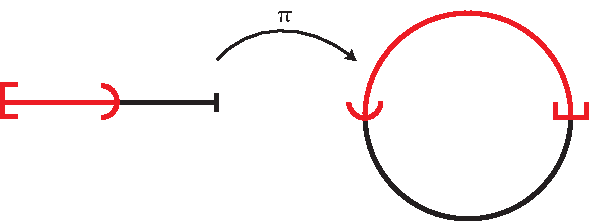
\includegraphics[trim=0cm 0cm 0cm 0cm,clip,scale=0.9]{images/half_circle-eps-converted-to.pdf}
		\end{center}
	\vspace{-6mm}
\end{example}
%riguardare come mettere l'immagine
\begin{observe}
	Gli omeomorfismi sono identificazioni chiuse e aperte.
\end{observe}
Vediamo ora che relazione c'è fra le identificazioni ed i quozienti dati da relazioni di equivalenza.
\begin{theorema} \textsc{proprietà universale delle identificazioni, Manetti, 5.6} \\
	\begin{minipage}[t]{0.83\textwidth}
		Dati $X,Y,Z$ spazi topologici, $g$ una qualsiasi funzione continua, \\
		$f$ identificazione con le mappe come in figura, allora \\
		$\exists ! h \text{ continua } \colon g=h\circ f \iff \left( \forall x,y\in X, \ f(x)=f(y)\implies g(x)=g(y)  \right)$ \\
		ovvero se e solo se $g$ è costante sulle fibre di $f$.
	\end{minipage}
	\begin{minipage}[t]{0.13\textwidth}\vspace{-10pt}
		\begin{tikzcd}
			X \arrow[r, "f"] \arrow[d, "g"'] & Y \arrow[ld, "\exists ! h", dotted] \\
			Z  &    
		\end{tikzcd}
	\end{minipage}
\end{theorema}
\begin{demonstration}
	Idealmente se $f$ fosse invertibile definiremmo $h=g\circ f^{-1}$. Tuttavia l'invertibilità di $f$ non è fra le ipotesi, quindi si sfrutta al meglio l'ipotesi della suriettività e si considera una controimmagine tramite $f$ e se ne fa l'immagine tramite $g$, ovvero $y\in Y, \ h(y)\coloneqq g(x)$ con $x\in f^{-1}(y)$. Con questa costruzione $h$ è ben definita siccome $g$ sarà costante sulle fibre di $f$. \\
	Verifichiamo che $h$ è continua tramite la definizione:
		\begin{gather*}
			U\subseteq Z \text{ aperto }, \ h^{-1}(U)\subseteq Y \iff f^{-1}(h^{-1}(U))\subseteq X \text{ aperto} \iff g^{-1}(U)\subseteq X \text{ aperto}
		\end{gather*}
	Siccome $g$ è continua allora lo è anche $h$.
\end{demonstration}
\begin{minipage}[t]{0.83\textwidth}
Come conseguenza si ha che, data $f$ continua, $\sim$ relazione di equivalenza e $\nicefrac{X}{\sim}$ spazio topologico con la topologia quoziente indotta dalla proiezione $\pi$, $\exists g$ continua $\iff \left( x\sim y \implies f(x)=f(y) \right)$, ovvero $\pi$ è costante sulle fibre di $f$.
\end{minipage}
\begin{minipage}[t]{0.16\textwidth}\vspace{-10pt}
 		\begin{tikzcd}
		 	X \arrow[r, "f"] \arrow[d, "\pi"']                                   & Y \\
 			\nicefrac{X}{\sim} \arrow[ur, "g"', dotted] &    
		\end{tikzcd}
	\end{minipage}\\
\hspace{-1mm}
\begin{minipage}[t]{0.83\textwidth}\vspace{2mm}
In particolare, se $\sim$ è la relazione d'equivalenza indotta da $f$, e dunque si è nelle ipotesi del primo Teorema fondamentale di isomorfismo degli \textit{insiemi}, allora $\left( x\sim y \iff f(x)=f(y) \right) \implies \exists ! \overline{f}$ biettiva, continua. Dunque vale 
		\begin{equation}
				\overline{f} \text{ omeomorfismo} \iff f \text{ identificazione}
			\end{equation}
	 	\end{minipage}
	\begin{minipage}[t]{0.16\textwidth}\vspace{1mm}
			\begin{tikzcd}
				X \arrow[r, "f"] \arrow[d, "\pi"']                                   & Y \\
				\nicefrac{X}{\sim} \arrow[ur, "\overline{f}"', dotted] &    
			\end{tikzcd}
	\end{minipage}\vspace{3mm}\\
Riprendiamo l'esempio precedente ed esaminiamolo in termini di spazio quoziente.
\begin{example}~{$\nicefrac{D^n}{\sim}\cong S^n$}\\
	Consideriamo il caso $n=1$:
	\begin{equation*}
		\funztot f {D^1=[0, \ 2\pi]} {S^1} t {(\cos t, \ \sin t)}
	\end{equation*}
	La funzione $f$ è un identificazione, dunque $S^1\cong \nicefrac{[0, \ 2\pi]}{\sim}\cong \nicefrac{[0, \ 1]}{\sim}=\nicefrac{D^1}{\sim}$, con $\sim$ tale che sia costante sulle fibre di $f$: 
	\begin{equation*}
		 s\sim t \iff \begin{cases} 
			\cos s=\cos t \\
			\sin s =\sin t
		\end{cases} \iff s=t  \vee s=0,\ t=2\pi
	\end{equation*} \newline
	Si può generalizzare in dimensione $n$ con l'identificazione:
	\begin{equation*}
		\funztot f {D^n} {S^n} x {\left( 2x\sqrt{1- \| \underline{x} \|^2}, \ 2\| \underline{x}\|^2 -1 \right)}
	\end{equation*}
	Dunque $\nicefrac{D^n}{\sim}\cong S^n$ per la relazione:
\begin{equation*}
	\underline{x}\sim \underline{y} \iff \underline{x}=\underline{y} \vee \labs \underline{x} \rabs ^2 = 1 = \| \underline{y} \| ^2
\end{equation*}
	In altre parole, ogni punto interno è \textit{in relazione con sé stesso} e tutti i punti sul bordo sono \textit{identificati} in un unica classe.
\end{example}
	
%LEZ 12
	\subsection{Quozienti tipici}
Vedremo ora degli esempi di spazi quoziente usati frequentemente.
\begin{intuit}
	Quando quozientiamo uno spazio topologico, possiamo immaginare che i punti contenuti nelle classi di equivalenza vengano ‘‘incollati'' tutti in un unico punto per formare un nuovo spazio quoziente.\\
	Ad esempio, prendendo il disco $D^2$ con la relazione di equivalenza $\sim$ che identifica i punti del bordo:
	\begin{equation*}
		(x_1,\ y_1) \sim (x_2,\ y_2)\iff (x_1,\ y_1)=(x_2,\ y_2) \text{ oppure } x_1^2 +y_1^2= x_2^2 +y_2^2=1
	\end{equation*} 
	I punti all'\textit{interno del disco} vengono tutti identificati in classi di equivalenza \textit{separate}, dunque passando allo spazio quoziente avremo una classe per \textit{ciascun} punto interno e un'\textit{unica} classe per tutti il bordo.\\
	Lo spazio quoziente ottenuto è $S^2$: possiamo ottenerlo visualmente ‘‘gonfiando'' l'interno del disco per poi chiudere il ‘‘palloncino'' ottenuto lungo i punti del bordo, come in figura.
	\begin{center}
		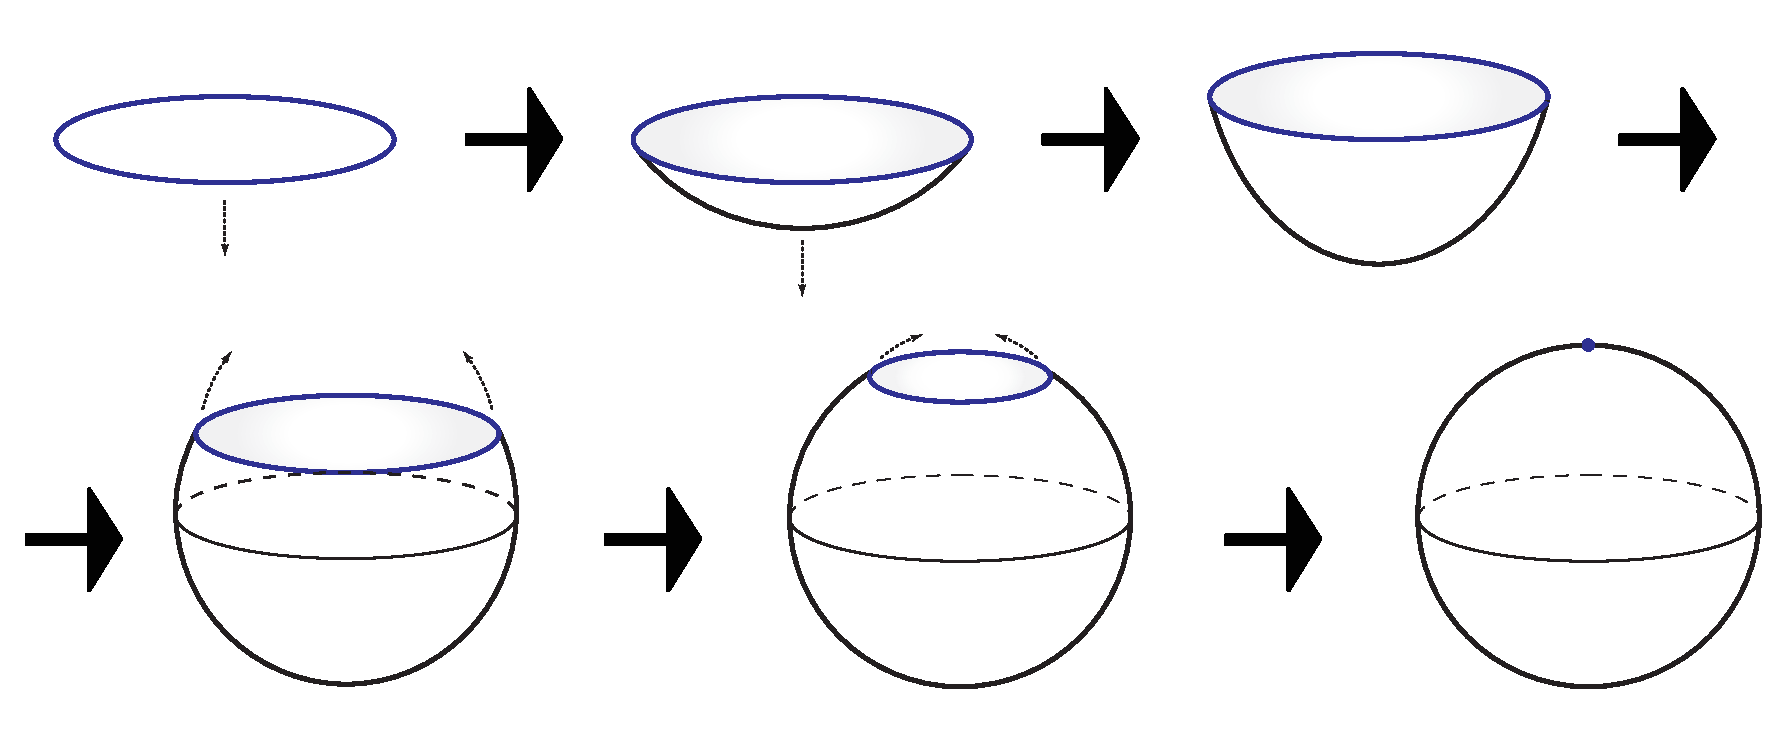
\includegraphics[trim=0cm 0cm 0cm 0cm,clip,scale=0.4]{images/disctosphere.pdf}
	\end{center}
\end{intuit}
\subsubsection{Contrazione di un sottospazio ad un punto}
Sia $X$ uno spazio topologico, $A\subseteq X$, $\forall x,y\in X \ x\sim y\iff x=y$ oppure $x,y\in A$, ovvero ogni punto è in relazione con sé stesso e tutti i punti di $A$ sono in relazione fra loro, dunque quozientando si ‘‘\textbf{contraggono}''\index{contrazione} ad un unico punto.
\begin{example} $\nicefrac{D^n}{S^{n-1}}\cong S^n$ \\
	Cerchiamo ora di generalizzare l'esempio precedente. Ricordiamo che relazione c'è fra i dischi e le sfere:
		\begin{gather*}
			D^n=\text{ disco in } \realset^n=\{\mathbf{x}\in\realset^n \mid \labs \mathbf{x} \rabs \leq 1 \}\\
			S^{n-1}=\text{ bordo di } D^n=\{\mathbf{x}\in\realset^n \mid \labs \mathbf{x} \rabs = 1 \}
		\end{gather*}
	Considerando $\sim$ come la contrazione di $S^{n-1}$ ad un punto, si ha che $\nicefrac{D^n}{S^{n-1}} \cong S^n$.
\end{example}

\begin{attention}
	Anche se $X$ è di \textbf{Hausdorff} non è detto che $\nicefrac{X}{A}$ sia di \textbf{Hausdorff}!\newline
	Se $A$ non è chiuso allora $\nicefrac{X}{A}$ non è neanche \textbf{T1}, infatti $\pi^{-1}([A])=A$ non chiuso implica che $[A]$ non lo è, quindi per la caratterizzazione degli spazi \textbf{T1} (definizione \ref{T1}, pag. \pageref{T1}) $\nicefrac{X}{A}$ non è \textbf{T1}.\newline 
	Tuttavia se $X$ è di \textbf{Hausdorff}, $K\subseteq X$ è compatto allora $\nicefrac{X}{K}$ è di \textbf{Hausdorff}.
\end{attention}
\subsubsection{Cono su uno spazio}
\begin{define}\textsc{Cilindro.}\\
	Dato $X$ spazio topologico, si definisce \textbf{cilindro}\index{cilindro} su $X$ lo spazio $X\times \intv$.
\end{define}
\begin{define}\textsc{Cono.}\\
	Il \textbf{cono}\index{cono} su $X$ spazio topologico è il quoziente $\displaystyle \nicefrac{X\times\intv}{X\times\{1\}}$ oppure $\displaystyle \nicefrac{X\times\intv}{X\times\{0\}}$.
\end{define}
\begin{intuit}
	Riprendendo il procedimento intuitivo di incollare parti dello spazio originale per creare il quoziente, lo stesso si può fare anche nel caso del cono. In questo caso, tutti i punti di una delle basi vengono incollati in uno.
\begin{center}
	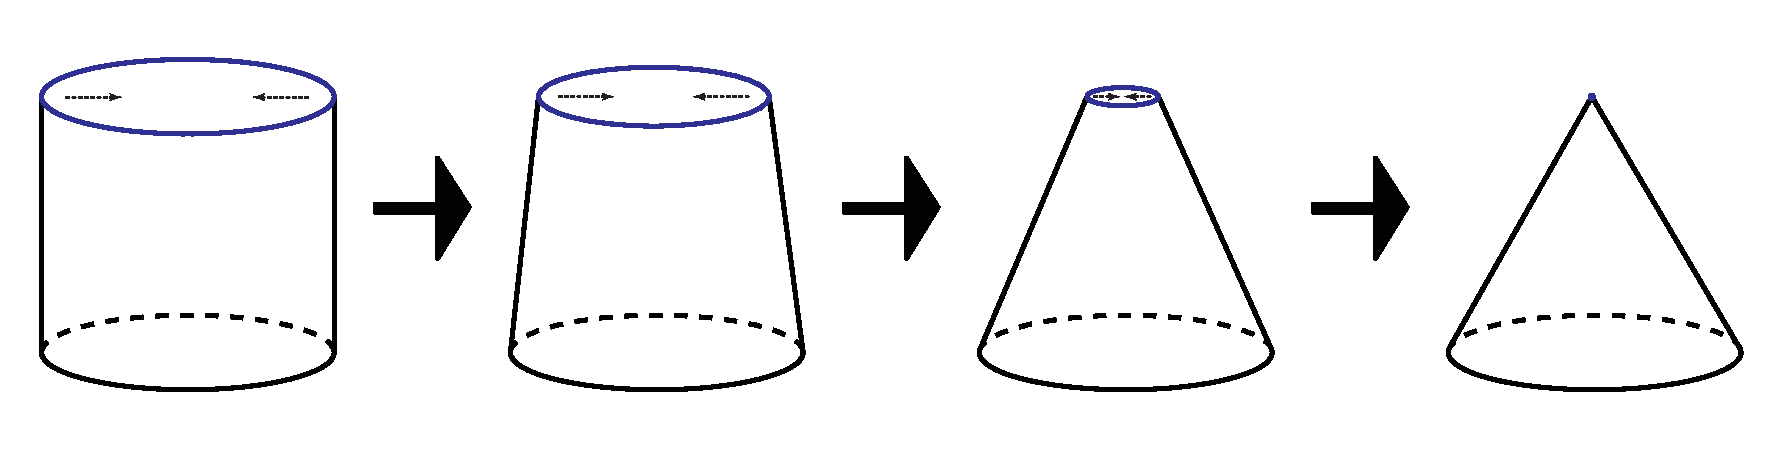
\includegraphics[trim=0cm 0cm 0cm 0cm,clip,scale=0.4]{images/cilindertocone.pdf}
\end{center}
\end{intuit}
\begin{observe}
	Un cono è sempre c.p.a. rispetto al ‘‘vertice''.
\end{observe}
\begin{example} \textsc{Cono su} $S^n \cong D^{n+1}$.\\
	Studiamo i casi al variare della dimensione.
	$n=0)$ $S^0=\{-1, \ 1\}=X \rightsquigarrow X\times\intv \rightsquigarrow \nicefrac{X\times\intv}{X\times \{1\}} \cong D^1$.
\begin{center}
	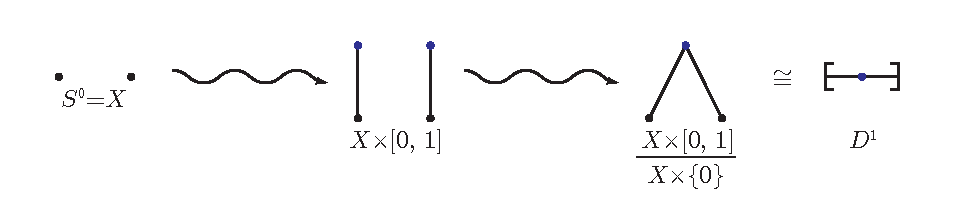
\includegraphics[trim=0cm 0cm 0cm 0cm,clip,scale=0.9]{images/cones0.pdf}
\end{center}
	$n=1)$ $S^1=X \rightsquigarrow X\times\intv \rightsquigarrow \nicefrac{X\times\intv}{X\times \{1\}} \cong D^2$.
\begin{center}
	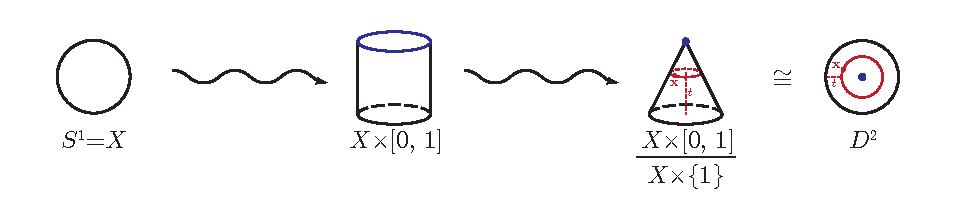
\includegraphics[trim=0cm 0cm 0cm 0cm,clip,scale=0.9]{images/cones1.pdf}
\end{center}
	In generale, considerata la funzione:
	\begin{equation*}
		\funztot f {S^n\times\intv} {D^{n+1}} {(\mathbf{x}, \ t)} {t\mathbf{x}}
	\end{equation*}
	Essa è continua, suriettiva, chiusa (compatto in \textbf{Hausdorff}), dunque $f$ è identificazione.\\
	Verifichiamo che la relazione di equivalenza indotta da $f$ è proprio quella di contrazione:
		\begin{gather*}
			(\mathbf{x}, \ t)\sim (\mathbf{y}, \ s) \iff f(\mathbf{x}, \ t)=f(\mathbf{y}, \ s) \iff t\mathbf{x}=s\mathbf{y} \iff \begin{cases} 
				\mathbf{x=y}, t=s \\ 
				t=s=0 
			\end{cases}\\
			\text{Se } t\neq 0 \implies \mathbf{x}=\frac{s}{t}\mathbf{y}, \text{ ma } \labs\mathbf{x}\rabs=1 \implies \left| \frac{s}{t} \right| \underbrace{\labs\mathbf{y}\rabs}_{=1}=1 \implies \left| \frac{s}{t} \right| =1 \implies s=t \implies \mathbf{x=y}
		\end{gather*}
	\vspace{-6mm}
\end{example}

\subsubsection{Retta con 2 origini}
Analizziamo un particolare spazio topologico che spesso fungerà da controesempio, in particolare per le varietà topologiche (vedi sezione   ): \textbf{la retta con 2 origini}. \newline
Sia $X=\realset\times\{a,b\}$.
%AAA SEZIONE CERCASI
\begin{center}
	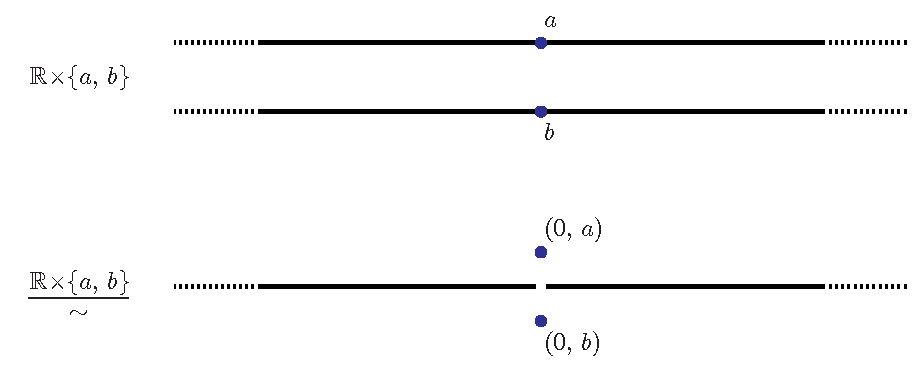
\includegraphics[trim=0cm 0cm 0cm 0cm,clip,scale=0.95]{images/line2origins.pdf}
\end{center}
Vogliamo definire una relazione di equivalenza che lasci ‘‘separate'' solo le origini:
	\begin{gather*}
		(x, \ \alpha)\sim (y, \ \beta) \iff 
			\begin{cases}
				x=y,\ \alpha=\beta \\
				x=y\neq 0
			\end{cases}		
	\end{gather*}
\textsc{Proprietà}
\begin{enumerate}
	\item $Y\coloneqq \nicefrac{X}{\sim}$ è c.p.a., infatti se i punti $(x, \ \alpha)$ e $(y, \ \beta)$ sono tali che $x\neq 0 \neq y$ basta prendere il segmento $\overline{xy}$ sulla retta $\realset\times\{a\}$ e proiettarlo. Per unire $(0,\ a)$ e $(0, \ b)$ basta unire entrambi con un cammino al punto $(1, \ a)=(1, \ b)$
	\item $Y$ non è di \textbf{Hausdorff}: tutti gli intorni di $(0, \ a)$ si intersecano con tutti gli 	intorni di $(0, \ b)$ 
	\item $Y$ è \textit{localmente omeomorfo} a $\realset$, infatti ogni punto ha un intorno omeomorfo ad un intervallo aperto di $\realset$
	\item $\exists K_1, K_2\subseteq Y$ compatti tali per cui $K_1\cap K_2$ \textit{non} è compatto: basta prendere $K_1=\pi\left([-1, \ 1]\times \{a\} \right)$ e $K_1=\pi\left([-1, \ 1]\times \{a\} \right)$ compatti in $Y$, ma $K_1\cap K_2= [-1,\ 0) \cup (0,\ 1]$ \textit{non} è compatto in $Y$
\end{enumerate}
\subsection{Quoziente Hausdroff}
Cerchiamo ora delle condizioni per avere un \textit{quoziente Hausdorff}.
\begin{theorema}
	Sia $\funz f X Y$ continua e identificazione con $X$ compatto e di \textbf{Hausdorff}, allora sono equivalenti:
		\begin{enumerate}
			\item $Y$ è di \textbf{Hausdorff}.
			\item $f$ chiusa.
			\item $K=\left\{ (x_1,\ x_2)\in X\times X \mid f(x_1)=f(x_2) \right\}$ chiuso in $X\times X$.
		\end{enumerate}
	\vspace{-3mm}
\end{theorema}
\begin{demonstration}
	$1 \implies 3)$  Si vuole utilizzare la caratterizzazione di essere \textbf{Hausdorff} con la chiusura della diagonale $\Delta_Y$, ovvero il teorema \ref{hausdorff diagonale chiusa}. Bisogna dunque vedere $K$ come controimmagine continua di $\Delta_Y$: si consideri	 $\funztot {h\coloneqq f\times f} {X\times X} {Y\times Y} {(x_1,\ x_2)} {\left( f(x_1), \ f(x_2) \right) }$ continua perché lo è $f$. Inoltre $K=h^{-1}(\Delta_Y)$ e $Y$ è $T_2 \implies K$ chiuso in quanto controimmagine di un chiuso tramite una funzione continua.
	\[ 	\begin{tikzcd}
				X \arrow[rrrr, "f"] &                                                                          &  &                                                       & Y \\
				& X\times X \arrow[rr, "h=f\times f" ,dotted] \arrow[lu, two heads] \arrow[ld, two heads] &  & Y\times Y \arrow[ru, two heads] \arrow[rd, two heads] &   \\
				X \arrow[rrrr, "f"] &                                                                          &  &                                                       & Y	
			\end{tikzcd} \]	
	$3\implies 2)$ Per dimostrare che $f$ è chiusa bisogna far vedere che $\forall C\subseteq X, C$ chiuso $\implies f(C)\subseteq Y$ chiuso, ma $f$ è identificazione $\iff f^{-1}\left( f(C) \right)\subseteq X$ chiuso. Notiamo che $f^{-1}\left( f(C) \right)= p_1(k\cap p_2^{-1}(C))$, infatti 
		\begin{gather*}
			p_2^{-1}(C)=X\times C \implies K\cap p_2^{-1}(C)= \left\{ (x_1,\ x_2)\in X\times X \mid f(x_2)\in C \right\}\\
			p_2 \text{ continua e $C$ chiuso } \implies p_2^{-1}(C) \text{ chiuso} \\
			K \text{ chiuso }\implies p_2^{-1}(C)\cap K \text{ chiuso}\\
			X \text{ compatto e } T_2 \implies p_1 \text{ chiuso}\implies p_1 \left( K\cap p_2^{-1}(C) \right) \text{ chiuso}
		\end{gather*}
	$2\implies 1)$ Serve il \textit{teorema di Wallace}, pertanto non ne affronteremo la dimostrazione.
\end{demonstration}
% SVN info for this file
\svnidlong
{$HeadURL$}
{$LastChangedDate$}
{$LastChangedRevision$}
{$LastChangedBy$}

\chapter{Azioni di gruppo}
\labelChapter{azionidigruppo}

\begin{introduction}
‘‘BEEP BOOP INSERIRE CITAZIONE QUA BEEP BOOP.''
\begin{flushright}
	\textsc{NON UN ROBOT,} UN UMANO IN CARNE ED OSSA BEEP BOOP.
\end{flushright}
\end{introduction}

\section{Azione di un gruppo su un insieme}
\begin{define}
	Sia $G$ un gruppo e $X$ un insieme. Si definisce il \textit{gruppo simmetrico} sull'insieme $X$ come $S(X)\coloneqq \{\funz f X X \mid f \text{ biunivoca}\}$. Un'\textit{azione} di $G$ su $X$ è
		\begin{itemize}
			\item  $\funz \Phi G {S(X)}$ morfismo di gruppi, ovvero $\Phi(g.h)=\phi(g)\Phi(h)$
			\item $\funztot \phi {G\times X} X {(g,\ x)} {g.x}$ t.c. $e.x=x, \forall x\in X$ e $g.(h.x)=(gh).x$
		\end{itemize}
	Se ho $\Phi$ definisco $\phi(g,\ x)=\underbrace{\Phi(g)}_{\in S(X)}(x)$.\newline
	Se ho $\phi$ definsco $\funztot {\Phi(g)} X X x {\phi(g,\ x)}$
\end{define}

\begin{define}
	Su $X$ definiamo una relazione che dimostreremo essere di equivalenza: $x\sim y\iff \exists g\in G \colon y=g.x$
\end{define}
Dimostrimo che è una relazione di equivalenza:
	\begin{itemize}
		\item riflessiva: $x=e.x$
		\item simmetrica: $y=g.x \implies x=g^{-1}.y$
		\item transitiva: $y=g.x,\ z=h.y \implies z=(hg).x$
	\end{itemize}
\begin{define}
	Le classi di equivalenza date da questa relazione sono dette \textit{orbite}
		\begin{gather*}
			[x]=G.x=\{y\in X \mid \exists y \colon y=g.x\}=\{ g.x\mid g\in G \}
		\end{gather*}
	L'insieme quoziente detto \textit{spazio delle orbite} si scrive come $\nicefrac{X}{G}$
\end{define}

Vediamo ora un esempio di azione e di orbite.
\begin{example}
	\begin{enumerate}
		\item $X=\realset^n, G=\gl(n,\ \realset), \ \phi(A,\mathbf{v})=A\mathbf{v}$ è la moltiplicazione matrice per vettore.\newline
		Analizziamo le orbite: $G.\mathbf{0}=\{\mathbf{0}\}$, ovvero il vettore nullo è un'orbita. Siano ora $\mathbf{v\neq 0\neq w}$. Esiste $A\in\gl(n,\ \realset) \colon \mathbf{w}=A\mathbf{v}$? Sì, se $\mathbf{v\neq 0}, G.\mathbf{v}=\realset^n\setminus\{\mathbf{0}\}$. \newline 
		Quindi $\nicefrac{\realset^n}{\gl(n, \realset)}=\{ a,\ b\}$ con $a=[\mathbf{0}]$ e $b=[\mathbf{v}], \mathbf{v\neq 0}$
	\end{enumerate}
\end{example}

%non ho scritto l'altro esempio perché l'ha ripreso CC, vedasi equazione 5.7

\section{Stabilizzatore di un elemento}
\begin{define}
Lo \textbf{stabilizzatore di un elemento}\index{stabilizzatore di un elemento} è l'insieme degli elementi di $G$ che fissano $x$:
\begin{equation}
H_x\coloneqq \left\{g\in G\mid g\ldotp x = x\right\}
\end{equation}
$H_x$ è un \textit{sottogruppo di isotropia} di $x$. Inoltre, se $H_x$ è banale, allora l'azione è \textbf{libera}\index{azione!libera}.
\end{define}
\begin{demonstration} $H_x$ è chiuso rispetto all'azione:
	\begin{itemize}
		\item $1_G\in H_x$ per definizione dell'azione $g\ldotp$ ($1_G\ldotp x=x\ \forall x$).
		\item $\forall g,\ h\in H_x$, allora $\left(gh\right)\ldotp x=g\ldotp \left(h\ldotp x\right)=g\ldotp x=x$.
	\end{itemize}
\end{demonstration}
\begin{observe}
L'insieme $\nicefrac{G}{H_x}$ dei laterali sinistri di $H_x$ in $G$ è in corrispondenza biunivoca con l'\textit{orbita} $O\left(x\right)$. Inoltre, se $G$ è finito, la cardinalità dell'orbita è pari all'indice di $H_x$ in $G$.
\end{observe}
\begin{demonstration}
Sia data:
\begin{equation*}
	\funztot{\alpha}{\nicefrac{G}{H_x}}{O\left(x\right)}{g\ldotp H_x}{g\ldotp x}
\end{equation*}
Mostriamo che $\alpha$ è ben definita e biunivoca.
\begin{enumerate}
	\item \textit{Ben definizione}: se $g\ldotp H_x=\tilde{g}\ldotp H_x$ allora $g^{-1}\tilde{g}=h\in H_x\implies\tilde{g}=gh\in H_x$. Si ha:
	\begin{equation*}
		\alpha\left(\tilde{g}\ldotp H_x\right)=\tilde{g}\ldotp x = \left(gh\right)\ldotp x = g \ldotp\left( h\ldotp x\right)=g\ldotp x=\alpha\left(g\ldotp H_x\right)
	\end{equation*}
 Poiché $g\ldotp H_x=\tilde{g}\ldotp H_x\implies g\ldotp x=\tilde{g}\ldotp x$ la funzione è ben definita.
 \item \textit{Iniettività}:
 \begin{align*}
 	\alpha\left(g_1\ldotp H_x\right)=\alpha\left(g_2\ldotp H_x\right)&\implies g_1\ldotp x=g_2\ldotp x\implies g_2^{-1}\ldotp\left(g_1\ldotp x\right)=g_2^{-1}\ldotp\left(g_2\ldotp x\right)\\
 	&\implies \left(g_2^{-1}\ldotp g_1\right)\ldotp x=1_G\ldotp x=x
 \end{align*}
Ne segue che $\left(g_2^{-1} g_1\right)\in H_x\implies g_2^{-1} g_1=h\in H_x\implies g_1\ldotp H_x=g_2\ldotp H_x$.
\item \textit{Suriettività}: se $y\in O\left(x\right)$, per definizione $\exists g\in G\ \colon y=g\ldotp x$, cioè $y=\alpha\left(g\ldotp H_x\right)$.
Ne consegue, dal teorema di Lagrange, che $\lvert O\left(x\right)\rvert = \left[G\ \colon H_x\right]= \frac{\lvert G\rvert}{\lvert H_x\rvert}$.
\end{enumerate}
\end{demonstration}
\begin{observe}
Punti nella stessa orbita hanno stabilizzatori \textbf{coniugati}\index{coniugati}\index{stabilizzatore di un elemento!coniugato}:
\begin{equation}
x_2=g\ldotp x_1\implies H_{x_2}=g\ldotp H_{x_1}\ldotp g^{-1}
\end{equation}
\end{observe}
\begin{demonstration}
$\includedx$ Sia $h\in H_{x_2}$. Si ha:
\begin{equation*}
h\ldotp x_2 = x_2\implies h\ldotp\left(g\ldotp x_1\right) = g\ldotp x_1 \implies \left(g^{-1} h g\right)\ldotp x_1 = x_1
\end{equation*}
Segue che $\forall h\in H_{x_2}\ g^{-1} h g\in H_{x_1}$, ma allora $h = g \left(g^{-1} h^{-1} g\right) g^{-1}\in g\ldotp H_{x_1}\ldotp g^{-1}$.
Pertanto per l'arbitrarietà di $h$ si ha $H_{x_2} \subseteq g \ldotp H_{x_1}\ldotp g^{-1} $\\
$\includesx$ Sia $h\in H_{x_1}$ e consideriamo $ghg^{-1}$. Se moltiplico (con l'azione $\ldotp$) per $x_2$:
\begin{equation*}
\left(ghg^{-1}\right)\ldotp x_2=\left(ghg^{-1}\right)\ldotp g\ldotp x_1=\left(gh\right)\ldotp \left(g^{-1}g\right)\ldotp x_1=\left(gh\right)\ldotp x_1=g\ldotp\left(h\right)\ldotp x_1=g\ldotp x_1=x_2
\end{equation*}
Pertanto $\forall h\in H_{x_1}\ \left(ghg^{-1}\right)\ldotp x_2= x_2$ e per l'arbitrarietà di $h$ si ha $g\ldotp H_{x_1}\ldotp g^{-1}\subseteq H_{x_2}$
\end{demonstration}
\section{Azione per omeomorfismi}
\begin{define}
Sia $X$ uno spazio topologico e $G$ un gruppo che agisce su $X$. Diciamo che $G$ \textbf{agisce per omeomorfismi}\index{azione!per omeomorfismi} se $\forall g\in G$ l'applicazione:
\begin{equation}
\funztot{\theta_g}{X}{X}{x}{g\ldotp x}
\end{equation}
è un \textit{omeomorfismo}.\\
Questo è equivalente a chiedere che l'azione sia data da un \textit{omomorfismo} di gruppi:
\begin{equation}
\funz{\Phi}{G}{\left\{\text{omeomorfismi } X\rightarrow X\right\}}\leq S\left(x\right)
\end{equation}
\end{define}
\begin{exercise}
 $G$ agisce per omeomorfismi se e solo se $\theta_g$ è continua $\forall g\in G$.
\end{exercise}
\begin{demonstration}
	...
\end{demonstration}
\begin{proposition}~{}
\begin{enumerate}
\item Sia $X$ uno spazio topologico e $G$ un gruppo che agisce su $X$ per omeomorfismo. Sia $\pi$ la proiezione dall'insieme allo spazio delle orbite $\nicefrac{X}{G}$:
	\begin{equation}
		\funz{\pi}{X}{\nicefrac{X}{G}}
	\end{equation}
Allora $\pi$ è aperta e, se $G$ è finito, $\pi$ è anche chiusa.
\item Sia $X$ di \textbf{Hausdorff} e $G$ gruppo finito che agisce su $X$ per omeomorfismi. Allora $\nicefrac{X}{G}$ è di Hausdorff.
\end{enumerate}
\end{proposition}
\begin{demonstration}~{}
\begin{enumerate}[label=\Roman*]
\item Sia $A\subseteq X$ un aperto. Vogliamo dimostrare che $\pi\left(A\right)$ è aperto in $\nicefrac{X}{G}$. Un aperto della topologia quoziente è tale se la controimmagine dell'aperto nel quoziente è un aperto: si deve allora dimostrare che $\pi^{-1}\left(\pi\left(A\right)\right)$ è aperto in $X$.\\
Ogni elemento di $A$ è contenuto in un orbita, dunque $\pi\left(A\right)$ contiene le orbite degli $x\in A$; la controimmagine $\pi^{-1}\left(\pi\left(A\right)\right)$ risulta dunque pari all'unione di \textit{tutte} le orbite in $X$ che intersecano l'insieme $A$:
\begin{equation*}
\pi^{-1}\left(\pi\left(A\right)\right)=\union_{g\in G} g\ldotp A
\end{equation*}
Ma allora $g\ldotp A=\left\{g\ldotp x\mid x\in A\right\}$ è un aperto $\forall g\in G$ poiché un omeomorfismo porta aperti in aperti; l'unione di aperti è aperta, dunque $\pi^{-1}\left(\pi\left(A\right)\right)$ è aperto in $X$ cioè $\pi\left(A\right)$ è aperto in $\nicefrac{X}{G}$.\\
Preso $C$ chiuso, dobbiamo allo stesso modo dimostrare $\pi\left(C\right)$ chiuso in $\nicefrac{X}{G}$, cioè $\pi^{-1}\left(\pi\left(C\right)\right)$ chiuso in $X$. Usando lo stesso ragionamento, otteniamo che:
\begin{equation*}
	\pi^{-1}\left(\pi\left(C\right)\right)=\union_{g\in G} g\ldotp C
\end{equation*} 
Con $g\ldotp C=\left\{g\ldotp x\mid x\in C\right\}$ chiuso per omeomorfismo. In particolare, essendo $G$ finito, segue che l'unione dei $g\ldotp C$ è finita e dunque anch'essa è un chiuso. Segue dunque $\pi^{-1}\left(\pi\left(C\right)\right)$ chiuso in $X$ e $\pi\left(C\right)$ chiuso in $\nicefrac{X}{G}$.
\item Siano $p,\ q\in \nicefrac{X}{G}$ distinti. Vogliamo dimostrare che esistono intorni di $p$ e $q$ disgiunti.\\
Siano $x,\ y\in X$ tali che $\pi\left(x\right)=p$ e $\pi\left(y\right)=q$ e consideriamo il gruppo finito $G=\left\{g_1=1_G,\ g_2,\ \ldots,\ g_n\right\}$. Le orbite di $x$ e $y$ sono diverse: se così non fosse, si avrebbe $\pi\left(x\right)=\pi\left(y\right)$ e cioè $p=q$, il che è assurdo! Allora:
\begin{equation*}
g_i\ldotp x\neq g_y\ldotp y\quad \forall i,\ j
\end{equation*}
Definiti gli (intorni) aperti $U\in I\left(x\right)$ e $V\in I\left(x\right)$ disgiunti (in quanto $X$ di \textbf{Hausdorff}), possiamo considerare gli altri (intorni) aperti disgiunti $g_i\ldotp U\in I\left(g_i\ldotp x\right),\ g_i\ldotp V\in I\left(g_i\ldotp y\right)$.\\
Allora:
\begin{equation}
\tilde{U}\coloneqq \union_{i}g_i\ldotp U\qquad \tilde{V}\coloneqq \union_{i}g_i\ldotp V
\end{equation}
Sono entrambi aperti. Vogliamo costruire $U\in I\left(x\right)$ e $V\in I\left(x\right)$ in modo che siano (intorni) aperti disgiunti tali che, costruiti come sopra $\tilde{U},\ \tilde{V}$, si abbia $\tilde{U}\cap \tilde{V}=\emptyset$. Così, passando al quoziente con $\pi$, si otterranno degli intorni $\pi\left(\tilde{U}\right)$ di $p$ e $\pi\left(\tilde{V}\right)$ di $q$ che soddisfano $\pi\left(\tilde{U}\right)\cap \pi\left(\tilde{V}\right)=\emptyset$.\\
\begin{itemize}
\item Costruiamo $U$ e $V$: $\forall i$ sappiamo che $x\neq g_i\ldotp y$ in $X$ (in quanto le orbite di $x$ e $y$ sono distinte. In quanto $X$ è di \textbf{Hausdorff}, si ha che $\forall i\ \exists U_i,\ V_i$ (intorni) aperti disgiunti tali che $x\in U_i$ e $g_i\ldotp y\in V_i$. Notiamo che $y\in g_i^{-1}\ldotp V_i$; allora definiamo
\begin{equation*}
U\coloneqq \inter_{i}^{n}U_i\in I\left(x\right)\qquad V\coloneqq \inter_{i=1}^{n}g_i^{-1}\ldotp V_i\in I\left(y\right)
\end{equation*}
\item Ricaviamo $\tilde{U}$ e $\tilde{V}$: $\forall i$ (e quindi per ogni elemento di $G$) abbiamo:
\begin{equation*}
U\cap \left(g_i\ldotp V\right)\subseteq U_i\left(g_i\ldotp g_i^{-1}\ldotp V_i\right)=U_i\cap V_i=\emptyset\implies U\cap \left(g_i\ldotp V\right)=\emptyset
\end{equation*}
Allora $\forall i,\ j$ abbiamo:
\begin{equation*}
	\left(g_i\ldotp U\right)\cap \left(g_j\ldotp V\right)=\left(g_i\ldotp U\right)\cap \left(g_ig_i^{-1}g_j\ldotp V\right)= g_i\ldotp \left(U\cap \left(g_i^{-1}g_j\right)\ldotp V\right)
\end{equation*}
Ma $g_i^{-1}g_j \in G$, dunque $U\cap \left(g_i^{-1}g_j\right)\ldotp V=\emptyset$. Segue che:
\begin{equation*}
	\left(g_i\ldotp U\right)\cap \left(g_j\ldotp V\right)=\emptyset\implies
	\left(\union_{i}g_i\ldotp U\right)\cap \left(\union_{i}g_i\ldotp V\right)=\emptyset\implies \tilde{U}\cap \tilde{V}=\emptyset
\end{equation*}	
\end{itemize}
\end{enumerate}
\end{demonstration}
\begin{example}
	$\left(\integerset,\ +\right)$ agisce in $\realset$ per \textbf{traslazione}\index{traslazione}:
	\begin{equation}
		m\ldotp x = x+m
	\end{equation}
Se mettiamo ad $\realset$ la topologia Euclidea, allora l'azione è per omeomorfismi, dato che fissato $m\in \integerset$: $\funztot{\theta_m}{\realset}{\realset}{x}{x+m}$ è continua.
\begin{itemize}
	\item \textit{Orbite}: $O\left(x\right)=\left\{x+m\mid m\in \integerset\right\}$ rappresenta tutti i numeri che hanno mantissa uguale (ad esempio, preso $x=1.5$, nella sua orbita abbiamo $1.5,\ 2.5,\ -1.5,\ 25.5,\ \ldots$).
	\item \textit{Stabilizzatore}: $H_x=\left\{m\in Z\mid x+m=x\right\}=\left\{0\right\}$ è banale, dunque l'azione è libera.
	\item \textit{Spazio delle orbite}: $\nicefrac{\realset}{\integerset}$ è insiemisticamente in corrispondenza biunivoca con $\left[0,\ 1\right)$, in particolare un sistema di rappresentanti di $\nicefrac{\realset}{\integerset}$ sono le orbite al variare di $x\in[0,1)$. Inoltre, lo spazio delle orbite è compatto essendo immagine continua di un compatto ($\pi\left(\left[0,\ 1\right]\right)=\nicefrac{\realset}{\integerset}$). Si può dimostrare che è omeomorfo a $S^1$.
\end{itemize}
\end{example}
\begin{demonstration}
Consideriamo $\funztot{f}{R}{S^1\subseteq \realset}{t}{\left(\cos\left(2\pi t\right),\sin\left(2\pi t\right)\right)}$.
\begin{itemize}
\item $f$ è continua.
\item $f$ è suriettiva.
\item $f\left(t_1\right)=f\left(t_2\right)\iff t_1-t_2\in \integerset \iff t_1,\ t_2$ nella stessa orbita$\iff \pi\left(t_1\right)=\pi\left(t_2\right)$
\end{itemize}
Allora la relazione di equivalenza indotta da $f$ è quella dell'azione di $\integerset$ su $\realset$.\\
\begin{minipage}[t]{0.83\textwidth}
 Inoltre, $f$ induce $\funz{\overline{f}}{\nicefrac{\realset}{\integerset}}{S^1}$ continua per le proprietà della topologia quoziente e che rende commutativo il diagramma a lato.
 Infatti $\overline{f}$ è biunivoca in quanto suriettiva (lo è $f$) ed iniettiva (per conseguenza del sistema di rappresentanti che si ha su $\nicefrac{\realset}{\integerset}$).
\end{minipage}
\begin{minipage}[t]{0.13\textwidth}\vspace{-10pt}
\begin{tikzcd}
	\realset \arrow[r, "f"] \arrow[d, "\pi"']                                   & S^1 \\
	\nicefrac{\realset}{\integerset} \arrow[ru, "\exists\overline{f}"', dotted] &    
\end{tikzcd}
\end{minipage}\\
Inoltre, essendo $\nicefrac{\realset}{\integerset}$ compatto ed $S^1$ di \textbf{Hausdorff}, $\overline{f}$ è chiusa e dunque $\overline{f}$ è l'\textit{omeomorfismo} cercato. Per questo motivo, si ha anche che $f$ è un'\textit{identificazione} aperta.
\end{demonstration}
\begin{digression}\label{complessir2}
	Si può sempre vedere $\realset^2$ come lo spazio dei complessi $\complexset$. Allora $S^1\in \complexset\implies S^1=\left\{z\mid \lvert z\rvert=1\right\}$. La funzione di prima si può anche riscrivere come:
	\begin{gather}
		\left(\cos\left(2\pi t\right),\sin\left(2\pi t\right)\right)\leftrightarrow \cos\left(2\pi t\right)+i\sin\left(2\pi t\right)\leftrightarrow e^{2\pi i t}
	\end{gather}
	\vspace{-8mm}
\end{digression}
\begin{example}
$G=GL\left(n,\ \realset\right)$ agisce su $\realset^n$ con l'azione di moltiplicazione matrice per vettore:
\begin{equation}
	A\ldotp \underline{v} = A\underline{v}
\end{equation}
L'azione è per omeomorfismi, dato che fissato $A\in G$: $\funztot{\theta_A}{\realset^n}{\realset^n}{\underline{v}}{A\underline{v}}$ è continua.
\begin{itemize}
	\item \textit{Orbite}: definite $O\left(\underline{v}\right)=\left\{A\underline{v}\mid A\in G\right\}$ ci sono solo due orbite, $\left[\underline{0}\right]$ e $\left[\underline{v}\right]$ con $\underline{v}\neq\underline{0}$, dato che ogni vettore può essere scritto come prodotto di un vettore per un'opportuna matrice di cambiamento di base.
	\item \textit{Spazio delle orbite}: $\nicefrac{\realset^n}{G}=\left\{\left[\underline{0}\right],\ \left[\underline{v}\right]\right\}$. Considerando la proiezione al quoziente $\funz{\pi}{\realset^n}{\nicefrac{\realset^n}{G}}$, si ha che $\pi^{-1}\left(\left[\underline{v}\right]\right)=\realset^n\setminus\left\{0\right\}$, che è un aperto ma \textit{non} è un chiuso. Per definizione di aperto della topologia quoziente $\left\{\left[\underline{v}\right]\right\}$ è aperto ma non chiuso in $\nicefrac{\realset^n}{G}$, dunque non tutti i punti nello spazio delle orbite son chiusi. Segue che $\nicefrac{\realset^n}{G}$ non è \textbf{T1} e tanto meno è di \textbf{Hausdorff}.
\end{itemize}
\end{example}
\begin{example}
	$G=\realset^{\ast}=\realset\setminus\left\{0\right\}$, inteso come gruppo moltiplicativo, agisce su $X=\realset^{n+1}\setminus\left\{0\right\}$ con l'azione di moltiplicazione per uno scalare:
	\begin{equation}
		\lambda\ldotp \underline{x} = \lambda\underline{x}
	\end{equation}
L'azione è per omeomorfismi, dato che fissato $\lambda\in G$: $\funztot{\theta_\lambda}{\realset^{n+1}\setminus\left\{0\right\}}{\realset^{n+1}\setminus\left\{0\right\}}{\underline{x}}{\lambda \underline{x}}$ è continua.
\begin{itemize}
	\item \textit{Orbite}: $O\left(\underline{x}\right)=\left\{\lambda \underline{x}\mid \lambda\in G\right\}$ rappresentano tutte le rette vettoriali passanti per l'origine in $\realset^{n+1}$ a cui son state tolte l'origine.
	\item \textit{Spazio delle orbite}: $\frac{\realset^{n+1}\setminus\left\{0\right\}}{G}=\mathbb{P}^n\left(\realset\right)$ è lo \textbf{spazio proiettivo reale}, spazio topologico rispetto alla topologia quoziente indotta dall'azione. $\mathbb{P}^n\left(\realset\right)$ è di \textbf{Hausdorff} e \textit{compatto}.
\end{itemize}
\end{example}
\begin{define} \label{def spazio proiettivo}
	Lo \textbf{spazio proiettivo reale}\index{spazio topologico!spazio proiettivo reale} $\mathbb{P}^n\left(\realset\right)$ (o $\realset\mathbb{P}^n$) di dimensione $n$ è lo spazio topologico delle rette vettoriali passanti origine in $\realset^{n+1}$, a cui son state tolte l'origine. È definito come lo spazio quoziente rispetto all'azione del gruppo moltiplicativo $\realset^{\ast}$:
	\begin{equation}
		\mathbb{P}^n\left(\realset\right)= \frac{\realset^{n+1}\setminus \left\{0\right\}}{\realset^{\ast}}
	\end{equation}
\end{define}
\begin{proposition}\label{spazi proiettivi compatti connessi}
$\mathbb{P}^n\left(\realset\right)$ è di \textbf{Hausdorff}, \textit{compatto} e \textbf{c.p.a.}.
\end{proposition}
\begin{demonstration}
\begin{enumerate}[label=\Roman*]
\item Dati $p,\ q\in\mathbb{P}^n\left(\realset\right)$, $p\neq q$ essi sono della forma $p=\left[\underline{x}\right]$ e $q=\left[\underline{y}\right]$. Allora:
\begin{equation*}
\left[\underline{x}\right]\neq\left[\underline{y}\right]\mathcal{L}_0\left(\underline{x}\right)\neq\mathcal{L}_0\left(\underline{y}\right)
\end{equation*}
Con $\mathcal{L}_0\left(\underline{x}\right),\ \mathcal{L}_0\left(\underline{y}\right)$ le rette vettoriali descritte da $\underline{x}$ e $\underline{y}$.\\
Prendiamo gli (intorni) aperti disgiunti $U\setminus{0}\in I\left(\underline{x}\right)$, $V\setminus{0}\in I\left(\underline{y}\right)$ in $\realset^{n+1}\setminus\left\{0\right\}$. Allora, passando al quoziente, $\pi\left(U\setminus{0}\right)$ e $\pi\left(V\setminus{0}\right)$ formano due fasci di rette a forma di ‘‘doppio cono infinito'' con vertice nell'origine; questi due coni sono (intorni) aperti in quanto
\begin{equation*}
\pi^{-1}\left(\pi\left(U\setminus{0}\right)\right)=U\setminus{0}\qquad\pi^{-1}\left(\pi\left(V\setminus{0}\right)\right)=V\setminus{0}
\end{equation*}
Inoltre sono intorni disgiunti di $p$ e $q$, dunque $\mathbb{P}^n\left(\realset\right)$ è di \textbf{Hausdorff}.
\item Per dimostrare che $\mathbb{P}^n\left(\realset\right)$ è compatto, mostreremo che $\pi\left(S^n\right)=\mathbb{P}^n\left(\realset\right)$, dato che $S^n\subseteq R^{n+1}\setminus\left\{0\right\}$ è compatto.\\
Notiamo che, presa l'orbita di un vettore $\underline{v}$, si ha:
\begin{equation*}
\left[\underline{v}\right]=\left\{\lambda \underline{v}\mid \lambda\in \realset^{\ast}\right\}=\left\{\underbrace{\lambda \lvert\lvert\underline{v}\rvert\rvert}_{=\mu\in \realset^{\ast}}\underbrace{\frac{\underline{v}}{\lvert\lvert\underline{v}\rvert\rvert}}_{\in S^1}\mid \lambda\in \realset^{\ast}\right\}=\left\{\mu \underline{x}\mid \mu\in \realset^{\ast}\right\}=\left[\underline{x}\right]
\end{equation*}
Dunque ogni orbita dello spazio proiettivo reale si può scrivere come l'orbita di un vettore appartenente alla sfera $S^n$. Segue che non solo $\pi$ è suriettiva, ma anche $\pi_{\mid S^n}$ è suriettiva, cioè $\pi_{\mid S^n}\left(S^n\right)=\mathbb{P}^n\left(\realset\right)$; segue dunque che $\pi\left(S^n\right)=\mathbb{P}^n\left(\realset\right)$. Dato che $S^n$ è compatto e \textbf{c.p.a.}, segue che anche lo spazio proiettivo reale è compatto e \textbf{c.p.a.} (in quanto immagine continua tramite $\pi$ di $S^n$).
\end{enumerate}
\end{demonstration}
% SVN info for this file
\svnidlong
{$HeadURL$}
{$LastChangedDate$}
{$LastChangedRevision$}
{$LastChangedBy$}

\chapter{Successioni}
\labelChapter{successioni}

\begin{introduction}
‘‘BEEP BOOP INSERIRE CITAZIONE QUA BEEP BOOP.''
\begin{flushright}
	\textsc{NON UN ROBOT,} UN UMANO IN CARNE ED OSSA BEEP BOOP.
\end{flushright}
\end{introduction}

\section{Numerabilità}
\begin{define}
Un insieme $X$ è \textbf{numerabile}\index{numerabile} se è finito oppure esiste una biezione tra l'insieme $X$ e i naturali $\naturalset$.
\end{define}
\begin{define}
Uno spazio topologico $X$ è \textbf{a base numerabile}\seeonlyindex{a base numerabile}{assioma di numerabilità!secondo} se esiste una base $\basis$ della topologia tale che $\basis$ sia numerabile. %sia di cardinalità numerabile??
Si dice anche che $X$ soddisfa il \textbf{secondo assioma di numerabilità}\index{assioma di numerabilità!secondo}.
\end{define}
\begin{define}
Uno spazio topologico $X$ è \textit{primo-numerabile}\seeonlyindex{primo-numerabile}{assioma di numerabilità!primo} se ogni punto ammette un sistema fondamentale di intorni che sia numerabile. Si dice anche che $X$ soddisfa il \textbf{primo assioma di numerabilità}\index{assioma di numerabilità!primo}.
\end{define}
\begin{observe}~{}
\begin{enumerate}
\item Il secondo assioma di numerabilità implica il primo.
\item Se $X$ è finito, $X$ soddisfa sempre i due assiomi.
\item Se $X$ è spazio metrico, $X$ è sempre \textit{primo-numerabile}.
\item Se $X$ è \textit{a base numerabile}, ogni sottospazio $Y$ di $X$ è \textit{a base numerabile}. In particolare $Y$ è primo-numerabile.
\item Se $X$ e $Y$ sono \textit{a base numerabile}, allora $X\times Y$ è \textit{a base numerabile}. In particolare $X\times Y$ è primo-numerabile.
\item Non è vero che il quoziente di $X$ spazio \textit{a base numerabile} (o \textit{primo-numerabile}) è sempre \textit{a base numerabile} (o \textit{primo-numerabile}).
\end{enumerate}
\end{observe}
\begin{demonstration}~{}
\begin{enumerate}[label=\Roman*]
	\item Se $X$ ha base numerabile $\basis$ e $x\in X$, allora $\left\{A\in \basis\mid x\in A\right\}$ è un sistema fondamentali di intorni di $x$ ed è chiaramente numerabile.
	\item Ogni base e sistema fondamentale di intorni contiene necessariamente un numero finito di elementi.
	\item Preso $x\in X$, allora $\left\{B_{\nicefrac{1}{n}}\left(x\right)\right\}_{n\in\naturalset}$ è un sistema fondamentale di intorni ed è numerabile.
	\item Se $\basis$ è una base numerabile per $X$, $\left\{A\cap Y\mid A\in \basis\right\}$ è base numerabile per $Y$.
	\item Se $\basis_X$ è una base numerabile per $X$ e $\basis_Y$ base numerabile per $Y$, allora $\left\{A\times B\mid A\in \basis_X,\ B\in\basis_Y\right\}$ è base di $X\times Y$ numerabile: il prodotto cartesiano di due insiemi numerabili rimane numerabile.
	\item La contrazione di $\integerset$ in $\realset$ ad un punto, cioè il quoziente $\nicefrac{\realset}{\integerset}$, non è primo-numerabile nè tanto meno a base numerabile, pur essendo $\realset$ a base numerabile in quanto metrico\footnote{Nelle ‘‘Note aggiuntive'', a pag. \pageref{dimostrazionenonnumerabilità}, si può trovare la dimostrazione di ciò.}.
\end{enumerate}
\end{demonstration}
\begin{example}
	$\realset$ con la topologia Euclidea è \textit{a base numerabile}. Presa infatti:
	\begin{equation*}
		\basis=\left\{\left(a,\ b\right)\mid a,\ b\in \rationalset,\ a<b\right\}
	\end{equation*}
	\begin{itemize}
		\item È numerabile (è definita con i razionali $\rationalset$, che sono numerabili)
		\item È una base perché, dati $x,\ y\in\realset,\ x<y$:
		\begin{equation*}
			\left(x,\ y\right)=\union_{\substack{a, b\in\rationalset\\ x<a<b<y}}\left(a,\ b\right)
		\end{equation*}
	\end{itemize}
\end{example}
\begin{proposition}
Sia $X$ \textit{a base numerabile}. Allora ogni ricoprimento aperto di $X$ ammette un sottoricoprimento numerabile.
\end{proposition}
\begin{demonstration}
Sia $\mathcal{A}$ un ricoprimento aperto di $X$, $\basis$ una base numerabile per $X$ e $x\in X$. Allora $\exists U_x\in\mathcal{A}$ tale che $x\in U_x$. Essendo $\basis$ base, $\exists B_x\in\basis$ tale che $x\in B_x\subseteq U_x$.\\
Abbiamo così determinato un sottoinsieme numerabile della base $\basis$:
\begin{equation*}
\tilde{\basis}\coloneqq\left\{B_x\mid x\in X\right\}
\end{equation*}
Allora esiste in particolare $E\subseteq X$ numerabile tale che:
\begin{equation*}
\tilde{\basis}\coloneqq\left\{B_x\mid x\in E\right\}
\end{equation*}
Se consideriamo ora $\tilde{\mathcal{A}}\coloneqq\left\{U_x\mid x\in E\right\}$, notiamo che:
\begin{itemize}
	\item $\tilde{A}\subseteq A$.
	\item $\tilde{A}$ è numerabile perché lo è $E$.
	\item $X=\union_{B_x\in\tilde{\basis}}B_x=\union_{x\in E}B_x\subseteq \union_{x\in E}U_x $.
\end{itemize}
Segue che $\tilde{\mathcal{A}}$ è un sottoricoprimento numerabile di $A$.
\end{demonstration}
\begin{define}
Uno spazio topologico $X$ si dice \textbf{separabile}\index{spazio topologico!separabile} se contiene un sottoinsieme $E$ \textit{denso} e \textit{numerabile}.
\end{define}
\begin{examples}~{}
	\begin{itemize}
		\item Se $X$ è numerabile, allora è separabile perché l'insieme stesso è un sottoinsieme numerabile e denso.
		\item $\realset^n$ con la topologia euclidea è separabile perché si ha $E=\rationalset^n$ denso in $\realset^n$.
	\end{itemize}
\end{examples}
\begin{lemming}\label{basenumseparabile}
Se $X$ è \textit{a base numerabile}, allora è \textit{separabile}.
\end{lemming}
\begin{demonstration}
	Sia $\basis$ una base numerabile. Per ogni $U\in\basis$ sia $x_U\in U$ un punto e sia:
	\begin{equation*}
		E=\left\{x_U\mid U\in \basis\right\}
	\end{equation*}
\begin{itemize}
	\item $E$ è numerabile perché lo è $\basis$: abbiamo preso un punto per ogni elemento della base numerabile.
	\item $E$ è denso: se $A\subseteq X$ è aperto \textit{non} vuoto, allora $\exists U\in\basis$ tale che $x_u\in U\subseteq A\implies x_U\in A\implies E\cap A\neq \emptyset$.
\end{itemize}
\end{demonstration}
\begin{proposition}
	Se $X$ è spazio metrico, $X$ è sempre primo-numerabile ed è:
	\begin{center}
		\textit{a base numerabile} $\iff$ \textit{separabile}
	\end{center}
\vspace{-8mm}
\end{proposition}
\begin{demonstration}~{}\\
$\impliesdx$ Sempre vera per ogni spazio anche non metrico (lemma \ref{basenumseparabile}).\\
$\impliessx$ Sia $E\subseteq X$ sottoinsieme numerabile e denso e consideriamo:
\begin{equation*}
	\basis=\left\{B_{\nicefrac{1}{n}}\left(e\right)\mid e\in E,\ n\in \naturalset\right\}
\end{equation*}
Questo insieme è numerabile: mostriamo che sia una base. Per far ciò fissiamo $U\subseteq X$ aperto e prendiamo $x\in U$: vogliamo trovare un aperto di $\basis$ contenuto in $U$ contenente $x$.\footnote{Gli elementi della base sono già aperti banalmente. Per l'arbitrarietà di $x$, troviamo un ricoprimento aperto di $U$ costituito da aperti di $\basis$ contenuto interamente in $U$, cioè $\displaystyle U=\union_{i\in I}B_i$.}\\
Sia $n\in\naturalset$ tale che $B_{\nicefrac{1}{n}}\left(x\right)\subseteq$. Cerchiamo opportuni $e\in E,\ m\in\naturalset$ tale che:
\begin{equation*}
x\in B_{\nicefrac{1}{m}}\left(e\right)\subseteq B_{\nicefrac{1}{n}}\left(x\right)\subseteq U
\end{equation*}
Consideriamo la palla $B_{\nicefrac{1}{2n}}\left(x\right)$. Siccome $E$ è denso in $X$, $\exists e\in E\cap B_{\nicefrac{1}{2n}}\left(x\right)$.\\
Prendiamo ora la balla $B_{\nicefrac{1}{2n}}\left(e\right)\in\basis$:
\begin{itemize}
	\item \textit{contiene} $x$ perché se $e\in B_{\nicefrac{1}{2n}}\left(x\right)\implies \mvf{d}{e}{y}<\frac{1}{2n}\implies x\in B_{\nicefrac{1}{2n}}\left(e\right)$
	\item $B_{\nicefrac{1}{2n}}\left(e\right)\subseteq B_{\nicefrac{1}{n}}\left(x\right)\subseteq U$; infatti, preso $y\in B_{\nicefrac{1}{2n}}\left(e\right)$ si ha:
	\begin{equation*}
		\mvf{d}{x}{y}\leq \mvf{d}{x}{e}+\mvf{d}{e}{y}<\frac{1}{2n}+\frac{1}{2n}=\frac{1}{n}
	\end{equation*}
$\implies y\in B_{\nicefrac{1}{n}}\left(x\right) \subseteq U$.
\end{itemize}
Segue la tesi.
\end{demonstration}
\begin{example}
	Si può vedere che $\realset^n$ è base numerabile anche perché è uno spazio metrico ed è separabile.
\end{example}
\begin{attention}
Un insieme con una certa topologia può essere a base numerabile (o primo-numerabile), ma non necessariamente rispetto ad un altra!
\end{attention}
\begin{example}
\textsc{Retta di Sorgenfrey}\index{retta di Sorgenfrey}.\\
Consideriamo $X=\realset$ con la topologia avente come base:
\begin{equation}
\basis=\left\{\left[a,\ b\right)\mid a,\ b\in\realset,\ a<b\right\}
\end{equation}
Mostriamo $\basis$ è base per una topologia, è separabile, primo-numerabile ma \textit{non} è a base numerabile.
\begin{itemize}
	\item \textit{Base per una topologia}: usiamo il teorema delle basi (Manetti, 3.7), pag. \pageref{teoremabasi}.
	\begin{enumerate}[label=\Roman*]
		\item $\displaystyle X=\union_{B\in \basis}B$ è ovvio.
		\item Prendiamo $A=\left[a,\ b\right),\ B=\left[c,\ d\right)$ e consideriamo:
		\begin{equation*}
			\forall x\in A\cap B=\left[\max\left\{a,\ b\right\},\ \min\left\{c,\ d\right\}\right)
		\end{equation*}
	Allora basta prendere $C=A\cap B\in\basis$ per soddisfare $x\in C\subseteq A\cap B$.
	\end{enumerate}
\item \textit{Separabile}: $E=\integerset$ è numerabile ed è denso perché vale sempre $\left[a,\ b\right)\cap \integerset \neq \emptyset$, dunque ogni aperto non vuoto interseca $E$; segue che $X$ è separabile.
\item \textit{Primo-numerabile}: s $a\in\realset$ allora $\left\{\left[a,\ a+\frac{1}{n}\right)\right\}_{n\in\naturalset}$ è un sistema fondamentale di intorni di $a$ numerabile. Preso $U$ intorno di $a$, $\exists b>a$ tale che $\left[a,\ b\right)\subseteq U$; inoltre, $\exists n\in\naturalset$ tale che $a+\frac{1}{n}<b$, cioè:
\begin{equation*}
\left[a,\ a+\frac{1}{n}\right)\subseteq\left[a,\ b\right)\subseteq U
\end{equation*}
\item \textit{Non a base numerabile}: presa una base $\tilde{\basis}$ per $X$, mostriamo che non è numerabile. Sia $x\in\realset$. Allora:
\begin{equation*}
\left[x,\ \infty\right)=\union_{y>x}\left[x,\ y\right)
\end{equation*}
È aperto. In particolare, esiste un aperto dipendente dal punto $x$, cioè $U\left(x\right)=\left[x,\ b\right)\in\tilde{\basis}$ (per un certo $b>x$) per cui $x\in U\left(x\right)\subseteq\left[x,\ \infty\right)$.\\
Notiamo che se $x\neq y$, allora $U\left(x\right)\neq U\left(y\right)$: preso $y>x$, segue che $x\notin \left[y,\ \infty\right)\supseteq U\left(y\right)\implies x\notin U\left(y\right)\implies U\left(x\right)\neq U\left(y\right)$. L'applicazione:
\begin{equation}
\funztot{\ }{\realset}{\tilde{\basis}}{x}{U\left(x\right)}
\end{equation}
\end{itemize}
è iniettiva, dunque $\tilde{\basis}$ non è in iniezione con i naturali e pertanto $\tilde{\basis}$ \textit{non} è numerabile.
\end{example}
\begin{center}
	\begin{tikzcd}
		&  & \begin{array}{c}
			\text{Primo}\\\text{numerabile}\end{array} \arrow[color=red, lld, "\text{se }X\text{ è metrico}"' six, shift right, below] \\
		\begin{array}{c}
			\text{A base}\\\text{numerabile}
		\end{array} \arrow[rrd, shift left, shorten >= 1em] \arrow[rru, shift right] &  &                                                                                      \\
		&  & \text{Separabile}                                                                   
	\end{tikzcd}
\end{center}
\section{Successioni}
\begin{define}
Una \textbf{successione}\index{successione} in uno spazio topologico $X$ è una funzione $\funz{a}{\naturalset}{X}$ che indichiamo con $\left\{a_n\right\}_{n\in\naturalset}=\left\{a_n\right\}$.
\end{define}
\begin{define}
Sia $\left\{a_n\right\}$ una successione in $X$. Diciamo che $\left\{a_n\right\}$ \textbf{converge}\index{convergenza} a $p\in X$ se $\forall U\in I\left(p\right)\ \exists n_0\in \naturalset\ \colon a_n\in U,\ \forall n\geq n_0$.
\end{define}
\begin{observe}
	Se $X$ è di \textbf{Hausdorff}, una successione convergente ha un \textbf{unico}\index{limite!unicità} limite.
\end{observe}
\begin{demonstration}
	Supponiamo che $\left\{a_n\right\}$ converga a $p$ e $q$. Mostriamo che $p=q$.\\
	Siano $U\in I\left(p\right)$ e $V\in I\left(q\right)$.
	\begin{itemize}
		\item Siccome $\left\{a_n\right\}$ converge a $p$, $\exists n_0$ tale che $a_n\in U \forall n\geq n_0$.
		\item Siccome $\left\{a_n\right\}$ converge a $1$, $\exists n_1$ tale che $a_n\in V \forall n\geq n_1$.
	\end{itemize}
\begin{equation*}
\implies a_n\in U\cap V\ \forall n\geq \max_{n_0,\ n_1}\implies U\cap V\neq \emptyset\implies p=q
\end{equation*}
L'ultima implicazione deriva dal fatto che $X$ è di \textbf{Hausdorff}. Infatti, se in \textbf{Hausdorff} $p\neq q\implies U\cap V = \emptyset$, vale anche la sua negazione: $U\cap V\neq \emptyset\implies p = q$.
\end{demonstration}
\begin{define}
Se $X$ è di \textbf{Hausdorff} e $\left\{a_n\right\}$ è convergente, ha senso parlare del \textbf{limite} della successione:
\begin{equation}
p=\lim_{n \to +\infty}a_n
\end{equation}
Se $X$ \textit{non} è di \textbf{Hausdorff}, la stessa successione può convergere a più punti, dunque non esiste il limite della successione.
\end{define}
\begin{examples}~{}
	\begin{itemize}
		\item Se $X$ ha la topologia banale $\topo=\left\{X,\ \emptyset\right\}$, l'unico intorno di qualunque punto è $X$. Allora ogni successione $\left\{a_n\right\}$ in $X$ converge sempre ad un qualunque punto $p$.
		\item Se $X$ ha la topologia discreta, $\left\{a_n\right\}$ successione in $X$ converge a $p\iff \exists n_0\ \colon a_n=p,\ \forall n\geq n_0$, cioè se la successione è finitamente costante. Infatti, nella topologia discreta anche il singoletto $\left\{p\right\}$ è intorno di $p$, dunque eventualmente la successione avrà solo termini nel singoletto.
	\end{itemize}
\end{examples}
\begin{observe}
Se $X$ spazio metrico:
\begin{equation}
	a_n\textsc{ converge a } p\iff \forall \epsilon>0\ \exists n_0\ \colon \mvf{d}{x}{y}<\epsilon,\ \forall n\geq n_0
\end{equation}
\vspace{-8mm}
\end{observe}
\begin{demonstration}~{}\\
	$\impliesdx$ $U=B_{\epsilon}\left(p\right)$ è l'intorno di convergenza che soddisfa l'implicazione.\\
	$\impliessx$ Sia $U\in I\left(p\right)$. Allora $\exists \epsilon\ \colon B_{\epsilon}\left(p\right)\subseteq U$. Ma allora, dato che per le ipotesi $\exists n_0\ \colon \mvf{d}{p}{a_n}<\epsilon,\ \forall n\geq n_0$, cioè $a_n\in B_{\epsilon}\left(p\right)\subseteq U\implies a_n\in U\forall n\geq n_0$.
\end{demonstration}
\subsection{Punti di accumulazione}
\begin{define}
	Un punto $p\in X$ è \textbf{punto di accumulazione per la successione}\index{punto di accumulazione!per una successione} $\left\{a_n\right\}$ se:
	\begin{equation}
		\forall U\in I\left(p\right),\ \forall N\in\naturalset\ \exists n\geq N\ \colon a_n\in U
	\end{equation}
\vspace{-8mm}
\end{define}
\begin{exercise}
	Se $X$ è spazio metrico, allora:
	\begin{equation}
		p\textsc{ punto di accumulazione per } a_n\iff \forall \epsilon>0\ \exists n_0\ \colon \mvf{d}{x}{y}<\epsilon,\ \forall n\geq n_0
	\end{equation}
\end{exercise}
\vspace{-8mm}
\begin{define}
	Un punto $p\in X$ è \textbf{punto di accumulazione per il sottoinsieme}\index{punto di accumulazione!per un sottoinsieme} $B\subseteq X$ se:
	\begin{equation}
		\forall U\in I\left(p\right), \exists b\in B \colon b\in U\setminus \left\{ p\right\}
	\end{equation}
L'insieme dei punti di accumulazione per il sottoinsieme $B$ è chiamato \textbf{derivato}\index{derivato} di $B$.
\end{define}
\begin{exercise}
Data la successione $\left\{a_n\right\}$ in $X$ e definito $A\coloneqq \{a_n\mid n\in\naturalset\}$:
\begin{itemize}
\item $p\in X$ punto di accumulazione per la successione non è mai punto di accumulazione per l'insieme $A$.
\item $p\in X$ punto di accumulazione per l'insieme $A$ in generale non è punto di accumulazione per la successione; se $X$ è metrico %
allora vale l'implicazione
\end{itemize}
\end{exercise}
\subsection{Sottosuccessioni}
\begin{define}
Una \textbf{sottosuccessione}\index{successione!sottosuccessione} di $\left\{a_n\right\}$ è la composizione di $\funz{a}{\naturalset}{X}$ con un'applicazione \textit{strettamente crescente} $\funztot{k}{\naturalset}{\naturalset}{n}{k\left(n\right)}$. Si indica con $\left\{a_{k_n}\right\}$.
\end{define}
\begin{lemming}\label{lemmatriangolino} $\textcolor{blue}{\circled{{\large \blacktriangle}}}$ 	Sia $\left\{a_n\right\}$ una successione su $X$ e $p\in X$. Valgono le seguenti implicazioni:
	\begin{equation}
		\circled{1}\ \left\{a_n\right\}\text{ converge a }p
	\end{equation}
\begin{equation*}
	\begin{array}{ll}
	\Downarrow 
\end{array}
\end{equation*}
\begin{equation}
		\circled{2}\ \left\{a_n\right\}\text{ ha una sottosuccessione convergente a }p
\end{equation}
\begin{equation*}
\begin{array}{ll}
	\Downarrow &  \textcolor{red}{\circled{\ast}}
\end{array}
\end{equation*}
\begin{equation}
	\circled{3}\ p\text{ è un punto di accumulazione per }\left\{a_n\right\}
\end{equation}
	\begin{equation*}
	\begin{array}{ll}
		\Downarrow & \textcolor{red}{\circled{\ast\ast}}
	\end{array}
\end{equation*}
\begin{equation}
	\circled{4}\ p\in\overline{A}\text{ dove }A=\left\{a_n\mid n\in \naturalset\right\}\subseteq X
\end{equation}
\end{lemming}~{}\\
\begin{demonstration}
$\circled{1}\implies\circled{2}$ La sottosuccessione convergente è la successione stessa.\\
$\circled{2}\implies\circled{3}$ Sia $\left\{a_{k\left(n\right)}\right\}$ una sottosuccessione convergente a $p$ e sia $U\in I\left(p\right)$. \\
Se $a_{k\left(n\right)}$ converge a $p$ si ha che $\exists n_0\ \colon a_{k\left(n\right)}\in U,\ \forall n\geq n_0$. Poichè $k\left(n\right)$ è strettamente crescente, $\exists n_1\ \colon k\left(n\right)\geq N,\ \forall n\geq n_1$. Allora preso:
\begin{equation*}
	n=\max\left\{n_0,\ n_1\right\}
\end{equation*}
Abbiamo che $a_{k\left(n\right)}\in U,\ k\left(n\right)\geq N$.\footnote{L'intorno $U$ è arbitrario.} Segue che $p$ è punto di accumulazione per $\left\{a_n\right\}$.\\
$\circled{3}\implies\circled{4}$ $p\in \overline{A}\iff \forall U\in I\left(p\right)\ A\cap U\neq \emptyset$. Allora sia $U$ intorno di $p$: voglia che $U\cap A\neq \emptyset$. Essendo $p$ punto di accumulazione per $\left\{a_n\right\}$, $\exists n\ a_n\in U\implies U\cap A\neq \emptyset$.
\end{demonstration}
\begin{lemming}\label{primonumesucc}
Sia $X$ \textit{primo-numerabile}, $\left\{a_n\right\}$ successione in $X$ e $p\in X$. Allora vale anche il viceversa di $\textcolor{red}{\circled{\ast}}$, cioè:
\begin{equation}
	\left\{a_n\right\}\text{ ha una sottosuccessione convergente a }p\iff p\text{ è di accumulazione per }\left\{a_n\right\}
\end{equation}
\end{lemming}
\begin{demonstration}
	$\impliesdx$ Vale per $\textcolor{red}{\circled{\ast}}$.\\
	$\impliessx$ Sia $\left\{U_m\right\}_{m\in\naturalset}$ sistema fondamentale di intorni di $p$ numerabile per ipotesi ($X$ primo-numerabile). Consideriamo i seguenti insiemi:
	\begin{equation*}
	\tilde{U}_m\coloneqq U_1\cap\ldots U_m\quad \forall m\in \naturalset
	\end{equation*}
\begin{itemize}
	\item $\tilde{U}_m$ è intorno di $p$, in quanto intersezione \textit{finita} di intorni di $p$.
	\item $\tilde{U}_m=U_1\cap\ldots U_m\supseteq U_1\cap\ldots U_m\cap U_{m+1}=\tilde{U}_{m+1}$.
\end{itemize}
Segue che $\left\{\tilde{U}_m\right\}$ è ancora un sistema fondamentale di intorni (numerabile) di $p$, infatti, se $V$ è intorno di $p$, $\exists m\ \colon V\supseteq U_m\supseteq \tilde{U}_m$.\\
A meno di sostituire $U_m$ con $\tilde{U}_m$, possiamo supporre che $U_1\supseteq U_2\supseteq U_3\supseteq \ldots$.\\
Costruiamo una sottosuccessione di $\left\{a_n\right\}$ convergente a $p$. Sicuramente:
\begin{itemize}
	\item $\exists k\left(1\right)\in \naturalset\ \colon a_{k\left(1\right)}\in U_1$.
	\item $\exists k\left(2\right)\geq k\left(1\right)+1\ \colon A_{k\left(2\right)}\in U_2$.
\end{itemize}
E così via: $\forall m\ \exists k\left(m\right)\geq k\left(m-1\right)+1$ tale che $a_{k\left(m\right)}\in U_m$, ottenendo una sottosuccessione $\left\{a_{k\left(m\right)}\right\}$. Notiamo in particolare che:
\begin{center}
\label{notasorridente} $\textcolor{blue}{{\large \smiley{}}}$ Se $m_2\geq m_1$, allora $a_{k\left(m_2\right)}\in U_{m_2}\subseteq U_{m_1}$.
\end{center}
Mostriamo che $\left\{A_{k\left(n\right)}\right\}$ converge a $p$.\\
Sia $V$ intorno di $p$. Dal sistema fondamentale di intorni $\exists m_0$ tale che $U_{m_0}\subseteq V$. Da $\textcolor{blue}{{\large \smiley{}}}$ si ha che $\forall m\geq m_0\ a_{k\left(m\right)}\in U_{m_0}\subseteq V$.
\end{demonstration}
\begin{proposition}
	\textsc{Caratterizzazione della chiusura in termini di successioni.}\\
	Sia $X$ uno spazio topologico \textit{primo-numerabile}. Sia $Y\subseteq X$ e $p\in X$. Sono equivalenti
	\begin{itemize}
		\item Esiste una successione in $Y$ convergente a $p$.
		\item $p$ è di accumulazione per una successione in $Y$.
		\item $p\in \overline{Y}$
	\end{itemize}
\end{proposition}
\begin{demonstration}~{}\\
$\circled{1}\implies\circled{2}$ Non è necessario che $X$ sia primo-numerabile, è immediato dal lemma \ref{lemmatriangolino} $\textcolor{blue}{\circled{{\large \blacktriangle}}}$ (pag. \pageref{lemmatriangolino}).\\
$\circled{2}\implies\circled{3}$ Non è necessario che $X$ sia primo-numerabile. Se $p$ di accumulazione per $\left\{a_n\right\}$ con $a_n\in y\ \forall n\implies A=\left\{a_n\mid n\in \naturalset\right\}\subseteq Y$. Allora segue dal lemma \ref{lemmatriangolino} $\textcolor{blue}{\circled{{\large \blacktriangle}}}$ (pag. \pageref{lemmatriangolino}) che $p\in A=\overline{\left\{a_n\mid n\in \naturalset\right\}}\subseteq \overline{Y}$ \\
$\circled{3}\implies\circled{1}$ Sia $\left\{U_n\right\}$ un sistmea fondamentale di intorni di $p$ tale che $U_n\supseteq U_{n+1}\ \forall n$. Allora:
\begin{equation*}
	p\in \overline{Y}\implies \forall n\ Y\cap U_n\neq\emptyset\implies\forall n\ \exists y_n\in Y\cap U_n
\end{equation*}
In modo analogo a $\textcolor{blue}{{\large \smiley{}}}$ (pag. \pageref{notasorridente}), se $n_2\geq n_1$, allora $y_{n_2}\in U_{n_2}\subseteq U_{n_1}$. Allora $\left\{y_n\right\}$ è una successione in $Y$, mostriamo che converge a $p$.\\
Sia $V$ intorno di $p$. Dal sistema fondamentale di intorni $\exists n_0$ tale che $U_{n_0}\subseteq V$. Dal ragionamento analogo a $\textcolor{blue}{{\large \smiley{}}}$ si ha che $\forall n\geq n_0\ y_n\in U_{n_0}\subseteq V$.
\end{demonstration}
\section{Successioni e compatti}
\begin{proposition}\label{compattocontenuto}\textsc{(Manetti, 4.46)}\\
Sia $X$ spazio topologico e sia $K_n\subseteq X\ \forall n\in\naturalset$ un sottospazio chiuso, \textit{compatto} e non vuoto. Supponiamo inoltre che:
\begin{equation*}
K_n\supseteq K_n+1\ \forall n\implies K_1\supseteq K_2\supseteq K_3\supseteq \ldots
\end{equation*}
Allora: $\inter_{n\geq 1}K_n\neq\emptyset$.
\end{proposition}
\begin{demonstration}
Iniziamo in $K_1$. Consideriamo $A_n\coloneqq K_1\setminus K_n$:
\begin{itemize}
	\item $K_n$ chiuso in $X\implies K_n$ chiuso in $K_1$. Allora $A_n$ completementare di un chiuso, dunque aperto in $K_1\ \forall m\geq 1$.
	\item $K_n\supseteq K_{n+1}\implies A_n\subseteq A_{n+1}\ \forall n\geq 1$.
\end{itemize}
Sia allora $N\in\naturalset$.
\begin{equation*}
	\union_{n=1}^{N}A_n=A_N=K_1\setminus \underbrace{K_N}_{\neq\emptyset}\subsetneqq K_1
\end{equation*}
Allora nessuna unione \textit{finita} degli $A_n$ ricopre $K_1$, cioè $\displaystyle \union_{n\in\naturalset}A_n\subsetneqq K_1$, altrimenti $\left\{A_n\right\}$ sarebbe un ricoprimento aperto di $K_1$ che \textit{non} ammette sottoricoprimento finito (assurdo, in quanto $K_1$ è \textit{compatto}!).
\begin{equation*}
\union_{n\geq 1}A_n=\union_{n\geq 1}K_1\setminus K_n=K_1\setminus \left(\inter_{n\geq 1}K_n\right)\subsetneqq K_1\implies \inter_{n\geq 1}K_n\neq\emptyset
\end{equation*}
\end{demonstration}
\begin{lemming}
In uno spazio topologico \textit{compatto} $X$ ogni successione in $X$ ha punti di accumulazione.
\end{lemming}
\begin{demonstration}
Sia	$\left\{a_n\right\}$ successione in $X$; per definizione:
\begin{center}
$p\in X$ punto di accumulazione per $\left\{a_n\right\}\iff \forall U\in I\left(p\right),\ \forall N\in\naturalset\ \exists n\geq N\ \colon a_n\in U$
\end{center}
Per $N$ fissato sia $A_N\coloneqq \left\{a_n\mid n\geq N\right\}\subseteq X$. Allora:
\begin{center}
	$p\in X$ punto di accumulazione per $\displaystyle\left\{a_n\right\}\iff \forall U\in I\left(p\right),\ \forall N\in\naturalset\ U\cap A_N\neq\emptyset\iff \forall N\in\naturalset,\ p\in\overline{A}_N\coloneqq C_N$
\end{center}
Dunque $\displaystyle\left\{\text{punti di accumulazione di} \left\{a_n\right\}\right\}=\inter_{N\in\naturalset}C_N$ e:
 \begin{center}
 	$\left\{a_n\right\}$ ha punti di accumulazione $\iff \inter_{N\in\naturalset}C_N\neq\emptyset$
 \end{center}
\begin{itemize}
	\item $A_B\neq \emptyset$ per definizione, dunque $C_N$ è un chiuso non vuoto.
	\item $X$ è compatto, $C_N$ chiuso in $X$ compatto $\implies C_N$ \textit{compatto}.
\end{itemize}
Poiché $A_N=\left\{a_n\mid n\geq N\right\}\supseteq A_ {N+1}=\left\{a_n\mid n\geq N+1\right\}$, si ha:
\begin{equation*}
C_N=\overline{A_N}\subseteq \overline{A_{N+1}}=C_{N+1}
\end{equation*}
Abbiamo trovato una successione di compatti contenuto l'uno nel successivo. Allora per la proposizione \ref{compattocontenuto} (pag. \pageref{compattocontenuto}, \textsc{(Manetti, 4.46)}). si ha che $\displaystyle\inter_{n\geq 1}C_N\neq \emptyset$.
Segue che esiste un punto di accumulazione per la successione.
\end{demonstration}
\subsection{Compattezza per successioni}
\begin{define}
Sia $X$ spazio topologico. $X$ si dice \textbf{compatto per successioni}\index{compatto!per successioni} se ogni successione ammette una sottosuccessione convergente.
\end{define}
\begin{observe}
Per il lemma \ref{lemmatriangolino} $\textcolor{blue}{\circled{{\large \blacktriangle}}}$ (pag. \pageref{lemmatriangolino}), se $X$ è compatto per successioni allora ogni successione in $X$ ha un punto di accumulazione.
\end{observe}
\begin{lemming}
	Sia $X$ \textit{primo-numerabile.} Allora:
\begin{enumerate}
	\item $X$ compatto per successioni $\iff $ Ogni successione in $X$ ha un punto di accumulazione.
	\item $X$ compatto $\implies$ $X$ compatto per successioni.
\end{enumerate}
\end{lemming}
\begin{demonstration}~{}
\begin{enumerate}[label=\Roman*]
\item $\impliesdx$ Vale per l'osservazione precedente.\\
$\impliessx$ Vale per il lemma \ref{primonumesucc}, pag. \pageref{primonumesucc}: se ogni successione ha un punto di accumulazione in $X$ primo numerabile, allora ogni sottosuccessione ammette una sottosuccessione convergente a $p$, cioè $X$ è compatto per successioni.
\item Se $X$ è compatto, allora ogni successione in $X$ ha dei punti di accumulazione e per il punto $1)$ segue che $X$ è compatto per successioni.
\end{enumerate}
\end{demonstration}
\begin{proposition}\textsc{Caratterizzazione della compattezza in termini di successioni}\\
	Sia $X$ uno spazio topologico a base numerabile. Allora sono equivalenti:
	\begin{enumerate}
		\item $X$ compatto.
		\item $X$ compatto per successioni
		\item Ogni successione in $X$ ammette un punto di accumulazione.
	\end{enumerate}
\end{proposition}
\begin{demonstration}
Sappiamo già che $2)\iff 3)$ e $1)\implies 2)$ dal lemma precedente. Dobbiamo dimostrare $2)\implies 1)$. Dimostriamo per contronominale ($\neg 1)\implies \neg 2)$): se $X$ \textit{non} è compatto, allora $X$ non è compatto per successioni, cioè esiste una sottosuccessione in $X$ che \textit{non} ha alcuna sottosuccessione convergente.\\
\begin{itemize}
	\item $X$ \textit{non} compatto$\implies \exists \tilde{\mathcal{A}}$ ricoprimento aperto di $X$ che \textit{non} ha sottoricoprimenti finiti.
	\item $X$ a \textit{base numerabile} $\implies\exists\mathcal{A}$ sottoricoprimento di $\tilde{\mathcal{A}}$ che sia numerabile.
\end{itemize}
Poiché ogni sottoricoprimento di $\mathcal{A}$ è anche un sottoricoprimento di $\tilde{\mathcal{A}}$, significa che $\mathcal{A}$ \textit{non} ha sottoricoprimenti finiti. Definiamo:
\begin{equation*}
\mathcal{A}\coloneqq\left\{A_n\right\}_{n\in\naturalset}
\end{equation*}
Allora:
\begin{equation*}
\forall n\in\naturalset\quad \union_{j=1}^n A_j\subsetneqq X\implies \exists x_n\in X\setminus \union_{j=1}^n A_j
\end{equation*}
Costruisco così una successione $\left\{x_n\right\}$ successione in $X$ tale per cui:
\begin{center}
	\label{notatriste} $\textcolor{red}{{\large \frownie{}}}$ $x_n\notin A_j\ \forall j\leq n$.
\end{center}
Mostriamo che $\left\{x_n\right\}$ non ha sottosuccessioni convergenti. Sia $\left\{x_{k\left(n\right)}\right\}$ una sottosuccessione arbitraria di $\left\{x_n\right\}$ e sia $p\in X$, mostriamo che essa non converga ad un qualunque $p$.\\
\begin{itemize}
	\item $\mathcal{A}$ è un (sotto)ricoprimento di $X\implies \exists N\ \colon p\in A_N$
	\item Da $\textcolor{red}{{\large \frownie{}}}$ (pag. \pageref{notatriste}) abbiamo che $x_n\notin A_N\ \forall n\geq N$ (dato che $x_n\not A_j\ \forall j\leq n$, in particolare in $A_N$ per ogni $n\geq N$); si ha allora $x_{k\left(n\right)}\notin A_n\ \forall n\ \colon k\left(n\right)\geq N$
\end{itemize}
Essendo $k\left(n\right)$ crescente, $\exists n_0\ \colon k\left(n\right)\geq N\ \forall n\geq n_0$. Segue che se $n\geq n_0$ allora $x_k\left(n\right)\notin A_N$ 
Poiché $A_N$ è intorno di $p$, segue che $\left\{x_{k\left(n\right)}\right\}$ non converge a $p$.
\end{demonstration}
\begin{theorema}
Sia $X$ spazio metrico. Allora:
\begin{equation}
	X\text{ compatto}\iff X\text{ compatto per successioni}
\end{equation}
\end{theorema}
\begin{center}
\begin{tikzcd}
	&  & \begin{array}{c}
		\text{Compatto per}\\ \text{successioni}
	\end{array}  \arrow[color=red, lld, "X\text{ a base numerabile}"' sixslant2, shift right, shorten <= 0.5em] \arrow[dd] \arrow[color=red, lld, "X\text{ metrico}" sixslant1, shift right, below, shorten <= 0.5em] \\
	\text{Compatto} \arrow[rrd, shift left, ] &  &                                                                                                                                                 \\
	&  & \begin{array}{c}
		\text{Ogni successione ha}\\ \text{un punto di accumulazione}
	\end{array} \arrow[color=red, uu, "\substack{\text{primo}\\\text{numerabile}}"' nine, shift right=4]                                     
\end{tikzcd}
\end{center}
\section{Spazi metrici completi}
\begin{define}
	Sia $\left(X,\ d\right)$ uno spazio metrico. Una successione $\left\{a_n\right\}$ si dice \textbf{di Cauchy}\index{successione!di Cauchy} se:
	\begin{equation}
		\forall \epsilon>0\ \exists n_0\in\naturalset\ \colon \mvf{d}{a_n}{a_m}<\epsilon,\ \forall n,\ m\geq n_0
	\end{equation}
\end{define}
\begin{define}
	Uno spazio metrico $\left(X,\ d\right)$ si dice \textbf{completo}\index{spazio topologico!metrico!completo} se ogni successione di Cauchy è convergente.
\end{define}
\begin{observe}~{}
	\begin{enumerate}
		\item Ogni successione \textit{convergente} è di \textit{Cauchy}.
		\item Una successione di Cauchy è \textit{convergente} se e solo se ha punti di accumulazione.
		\item Una successione di Cauchy è \textit{convergente} se ha una \textit{sottosuccessione convergente}.
		\item Se $X$ è \textit{compatto}, allora ogni successione di Cauchy è \textit{convergente}.
		\item Se $X$ è spazio metrico \textit{compatto}, allora $X$ è spazio metrico \textit{completo}; non è vero il viceversa.
	\end{enumerate}
\end{observe}
\begin{demonstration}~{}
	\begin{enumerate}[label=\Roman*]
		\item Se $a_n\to p$ per $n\to +\infty$ significa che:
		\begin{equation*}
			\forall \epsilon>0\ \exists n_0\in\naturalset\ \colon \mvf{d}{a_n}{p}<\epsilon,\ \forall n\geq n_0
		\end{equation*}
	Considerati $n,\ m\geq n_0$ si ha:
	\begin{equation}
		\mvf{d}{a_n}{a_m}\leq \mvf{d}{a_n}{p}+\mvf{d}{p}{a_n}< 2\epsilon
	\end{equation}
Per l'arbitrarietà di $\epsilon$ vale la convergenza.
\item $\impliesdx$ Sempre vera per  \ref{lemmatriangolino} $\textcolor{blue}{\circled{{\large \blacktriangle}}}$ (pag. \pageref{lemmatriangolino}).\\
$\impliessx$ Sia $\left\{a_n\right\}$ una successione di Cauchy e sia $p$ un punto di accumulazione. Sia $\epsilon>0$: dalla definizione di successione di Cauchy $\exists n_0$ tale per cui $\mvf{d}{a_n}{a_m}<\epsilon\ \forall n,\ m\geq n_0$.\\
Essendo $p$ di accumulazione, $\exists n_1\geq n_0$ tale per cui $\mvf{d}{p}{a_{n_1}}<\epsilon$. Allora, se $n\geq n_0$ si ha:
	\begin{equation*}
	\mvf{d}{a_n}{p}\leq \mvf{d}{a_n}{a_{n_1}}+\mvf{d}{a_{n_1}}{p}< 2\epsilon
\end{equation*}
Dunque $\left\{a_n\right\}$ converge a $p$.
\item Poiché $X$ è metrico, $X$ è primo-numerabile, dunque avere un punto di accumulazione è equivalente ad avere una sottosuccessione convergente.
\item Se $X$ è compatto, ogni successione ha punti di accumulazione, in particolare quelle di Cauchy: per il punto $2)$ tutte le successioni di Cauchy risultano allora convergenti.
\item Segue dal punto $4)$. Un controesempio del viceversa è $R^n$, dato che è completo ma non è compatto (si veda il teorema seguente). 
\end{enumerate}
\end{demonstration}
\begin{theorema}
	$\realset^n$ in metrica euclidea è uno spazio metrico completo.
\end{theorema}
\begin{demonstration}
	Sia $\left\{a_n\right\}$ di Cauchy in $\realset^n$. Mostriamo che $\left\{a_n\right\}$ è eventualmente limitata\footnote{Supponendo chiaramente che la successione sia ben definita, ci interessa solamente che la successione sia limitata dopo un $n_0$: prima di ciò ho un numero finito di termini $a_0,\ \ldots,\ a_{n_0}<\infty$ e posso chiaramente prendere una palla (chiusa) che li contenga, ad esempio di raggio $M+1$ con $M$ definito come nella dimostrazione.}.\\
	Poiché la successione di Cauchy è definita per ogni $\epsilon$, fissiamo $\epsilon=1$. Allora:
	\begin{equation*}
	\exists n_0\ \colon \lvert\lvert a_n-a_m\rvert\rvert\leq 1\ \forall n,\ m\geq n_0
	\end{equation*}
Sia $M\coloneqq \max_{n_0,\ \ldots,\ n_0}\lvert\lvert a_n\rvert\rvert$. Se $n\geq n_0$ si ha:
\begin{equation*}
\lvert\lvert a_n\rvert\rvert=\lvert\lvert a_n - a_{n_0}+ a_{n_0}\rvert\rvert=\leq \lvert\lvert a_n - a_{n_0}\rvert\rvert+\lvert\lvert a_{n_0}\rvert\rvert\leq 1+M
\end{equation*}
Questo significa che $\left\{a_n\right\}\subseteq\overline{B_{1+M}\left(0\right)}$. Questa palla chiusa è uno spazio metrico \textit{indotto} in $\realset^n$ e compatto, cioè è uno \textit{spazio metrico completo}. Allora la successione di Cauchy, trovandosi in uno spazio metrico completo, converge in esso, e dunque converge anche in $\realset^n$.
\end{demonstration}
\begin{attention}
La \textbf{completezza} \textit{non} è una proprietà topologica! Per esempio, $\realset$ e $\left(0,\ 1\right)$ con metrica euclidea sono omeomorfi rispetto alla topologia indotta dalla metrica, ma $\realset$ abbiamo appena dimostrato che è completo, mentre $\left(0,\ 1\right)$ si può vedere che non lo è!
\end{attention}
\part{Omotopia}
\labelPart{second}
% SVN info for this file
\svnidlong
{$HeadURL$}
{$LastChangedDate$}
{$LastChangedRevision$}
{$LastChangedBy$}

\chapter{Omotopia}
\labelChapter{omotopia}

\begin{introduction}
	‘‘Molto spesso si è ripetuto che la Geometria è l'arte di ragionare bene su figure mal fatte; in ogni caso queste figure, per non ingannarci, devono soddisfare determinate condizioni; le proporzioni
	possono essere grossolanamente distorte, ma le posizioni relative del
	le varie parti non devono essere interrotte.''
	\begin{flushright}
		\textsc{Henri Poincaré,} dopo aver finito di leggere il già citato libro di Topologia.
	\end{flushright}
\end{introduction}
\noindent Finora abbiamo visto omeomorfismi tra spazi topologici sotto tanti aspetti diversi, definendo rigorosamente quella che era l'intuizione del magico materiale elastico. Possiamo osservare tuttavia delle ‘‘\textit{equivalenze di forma}'' che un omeomorfismo è troppo rigido per descriverle.\\
Ad esempio, si possono considerare \textit{equivalenti} figure con lo stesso numero di buchi. Sotto questo punto di vista, la figura corrispondente alla lettera \textsf{\textbf{O}} e quella corrispondente a \textsf{\textbf{P}} sono \textit{equivalenti}, dato che hanno entrambe un solo buco, mentre \textsf{\textbf{X}} non lo è perché non ne ha. Allo stesso tempo, nessuna di queste è \textit{omeomorfa} all'altra: infatti, se togliamo dalle tre lettera/figure un punto come il nodo di raccordo delle ‘‘stanghette'' (o per \textsf{\textbf{O}} un punto qualunque), otteniamo per \textsf{\textbf{O}} una componente connessa, per \textsf{\textbf{P}} due e per \textsf{\textbf{X}} ben quattro distinte.\\
Preceduto da un'approfondimento delle componenti connesse (anche per archi), nel presente capitolo formalizzeremo questo tipo di equivalenza più debole e allo stesso tempo più ampia: l'\textbf{omotopia}.
\section{Lemma di incollamento}
\begin{lemming}[Lemma di incollamento.]~{}\label{lemmaincollamento}\\
Siano $X,\ Y$ spazi topologici e $X=A\cup B$. Siano $\funz{f}{A}{Y}$ e $\funz{g}{B}{Y}$ continue tali che $f\left(x\right)=g\left(x\right)\ \forall x\in A\cap B$, cioè $f_{\mid A\cap B}=g_{\mid A\cap B}$.\\
Consideriamo l'\textbf{incollamento}\index{incollamento} $\funz{h}{X}{Y}$ definito da:
	\begin{equation}
		h\left(x\right)=\begin{cases}
			f\left(x\right)\ x\in A\\
			g\left(x\right)\ x\in B
		\end{cases}
	\end{equation}
	Se $A$ e $B$ sono entrambi aperti in $X$ (o entrambi chiusi in $X$), allora $h$ è continua.
\end{lemming}
\begin{demonstration}
	Supponiamo $A$ e $B$ aperti. Sia $U\subseteq Y$ aperto. Allora:
	\begin{equation*}
		h^{-1}\left(U\right)=\underbrace{f^{-1}\left(U\right)}_{\subseteq A}\cap \underbrace{g^{-1}\left(U\right)}_{\subseteq B}
	\end{equation*}
Essendo $f,\ g$ continue, segue che $f^{-1}\left(U\right)$ è aperto in $A$ e $g^{-1}\left(U\right)$ è aperto in $B$.\\
In quanto $A,\ B$ aperti, per definizione di aperto del sottospazio\footnote{Poiché un aperto del sottospazio è dato dall'intersezione del sottospazio con un aperto di $X$, se abbiamo che anche il sottospazio è aperto di $X$, l'intersezione è aperta: in questo caso ogni aperto del sottospazio è anche aperto di $X$.} $f^{-1}\left(U\right)$ e $g^{-1}\left(U\right)$ sono aperti su $X\implies h^{-1}\left(U\right)$ aperto.\\
Il caso di $A$ e $B$ chiusi è esattamente analogo.
\end{demonstration}
\section{Componenti connesse e componenti c.p.a.}
Riprendiamo la trattazione delle componenti connesse e \textbf{c.p.a.} introdotte nel \autoref{chap:Connessocompatto}.
\begin{define}[Componente connessa.]~{}\\
	Una \textbf{componente connessa}\index{componente!connessa} di $X$ spazio topologico è uno spazio $C\subseteq X$ \textit{connesso} \textbf{massimale}, tale per cui:
	\begin{equation}
		C\subseteq A\subseteq X\text{ con }A\text{ connesso}\implies C=A
	\end{equation}
\vspace{-6mm}
\end{define}
\begin{observes}~{}
\begin{itemize}
	\item Le componenti connesse formano una \textit{partizione} di $X$.
	\item Se $x\in X$ si può definire la componente connessa che contiene $x$:
	\begin{equation}
		C\left(x\right)=\union\left\{C\subseteq X\mid x\in C,\ C\text{ connesso}\right\}
	\end{equation}
\item Le componenti connesse possono essere viste come classi di equivalenza per la seguente relazione di equivalenza su $ X $:
	\begin{equation}
		x,\ y\in X\qquad x\sim_C y\iff \exists C\subseteq X\text{ connesso}\ \colon x,\ y\in C
	\end{equation}
\end{itemize}
\vspace{-6mm}
\end{observes}
\begin{demonstration}
Innanzitutto mostriamo che la relazione è di equivalenza:
\begin{itemize}
\item \textsc{Riflessiva}: $x\sim_C x$ è vero, dato che $\left\{x\right\}$ è sempre un connesso.
\item \textsc{Simmetrica}: ovvia dalla definizione.
\item \textsc{Transitiva}: Supponiamo $x\sim_C y,\ y\sim_C z$. Allora $\exists C,\ D\subseteq X$ connessi tale che $x,\ y\in C$ e $y,\ z\in D$. Allora $C\cup D$ contiene sia $x$ che $z$. Inoltre, essendo $y\in C\cap D\implies C\cap D\neq \emptyset$, dunque $C\cup D$ è un connesso: vale $x\sim_C z$.\\
Mostriamo che le classi di equivalenza sono le componenti connesse per $x$.\\
$\includedx$ Se $C\subseteq X$ è una componente connessa, allora $\forall x, y\in C$ si ha $x\sim_C y$, cioè $C$ è interamente contenuta in $C_0=[x]=[y]$ classe di equivalenza per $\sim_C$: $C\subseteq C_0$.\\
$\includesx$ Sia $z\in C_0$ classe di equivalenza e sia $x\in C$ componente connessa. Allora: $x\sim_C z\implies \exists T\subseteq X \text{ connesso}\ \colon x,\ z\in T$.\\
Consideriamo $C\cup T$. $C$ e $T$ sono connessi, $x\in C\cap T\implies C\cap T\neq \emptyset$: $C\cup T$ è ancora connessa. In quanto $C$ è componente connessa, poiché $C\subseteq C\cup T$, per definizione segue che $C=C\cup T$, cioè $T\subseteq C$. Allora $z\in C$ e $C_0\subseteq C$.
\end{itemize}
\vspace{-3mm}
\end{demonstration}
\begin{define}[Componente c.p.a..]~{}\\
Una \textbf{componente c.p.a.}\index{componente!c.p.a.} di $X$ è una classe di equivalenza per la relazione $\sim_A$ così definita:
	\begin{equation}
	x,\ y\in X\qquad x\sim_A y\iff \exists \alpha\textsc{ cammino in }X\ \colon \alpha\left(0\right)=x,\ \alpha\left(1\right)=y
\end{equation}
\vspace{-6mm}
\end{define}
\begin{demonstration}
	Mostriamo che sia una relazione di equivalenza:
	\begin{itemize}
		\item \textsc{Riflessiva}: $x\sim_A x$ è vero, dato che esiste sempre il \textbf{cammino costante}\index{cammino!costante} nel punto $x$: \begin{equation}
			\funztot{c_x}{I}{X}{t}{x}
		\end{equation}
		\item \textsc{Simmetrica}: se $x\sim_A y$ sappiamo che $\exists\ \funz{\alpha}{I}{X}$ tale per cui $\alpha\left(0\right)=x,\ \alpha\left(1\right)=y$. Possiamo definire il \textbf{cammino inverso}\index{cammino!inverso}:
		\begin{equation}
			\funztot{\overline{\alpha}}{I}{X}{t}{\alpha\left(1-t\right)}
		\end{equation}
	\begin{itemize}
		\item $\overline{\alpha}$ è continuo, perché composizione di applicazioni continue:\\
		\begin{center}
			\begin{tikzcd}
				I \arrow[r]          & I \arrow[r, "\alpha"]  & X                      \\[-25pt]
				t \arrow[r, maps to] & 1+t \arrow[r, maps to] & \alpha\left(1-t\right)
			\end{tikzcd}
		\end{center}
	\item $\overline{\alpha}\left(0\right)=\alpha\left(1\right)=y,\ \overline{\alpha}\left(1\right)=\alpha\left(0\right)=x$.
	\end{itemize}
Allora il cammino $\overline{\alpha}$ definisce $y\sim_A x$.
		\item \textsc{Transitiva}: Supponiamo $x\sim_A y,\ y\sim_A z$. Allora $\exists \funz{\alpha,\ \beta}{I}{X}$ tale che $\alpha\left(0\right)=x,\ \alpha\left(1\right)=y, \beta\left(0\right)=y,\ \beta\left(1\right)=z$. Usando la \textbf{giunzione di cammini}\index{cammino!giunzione di cammini}:
	\begin{equation}
	\left(\alpha\ast\beta\right)\left(t\right)=\begin{cases}
		\begin{array}{lc}
					\alpha\left(2t\right) & \text{se }0\leq t\leq \frac{1}{2}\\
			\beta\left(2t-1\right) & \text{se }\frac{1}{2}\leq t\leq 1	
		\end{array}
	\end{cases}
\end{equation}
In particolare:
\begin{equation*}
	\begin{cases}
	\left(\alpha\ast\beta\right)\left(0\right)=\alpha\left(0\right)\\
	\left(\alpha\ast\beta\right)\left(1\right)=\beta\left(1\right)
		\end{cases}
\end{equation*}
Poiché $\alpha\ast\beta$ soddisfa le ipotesi del lemma di incollamento, essa è continua e collega con un cammino unico $x$ e $z$, dunque vale $x\sim_A z$.
	\end{itemize}
\end{demonstration}
\begin{observes}~{}
	\begin{enumerate}
		\item Le componenti \textbf{c.p.a.} formano una partizione di $X$
		\item Sia $C\subseteq X$ un sottospazio \textbf{c.p.a.} per cui vale che $C\subseteq A\subseteq X$ con $A$ \textbf{c.p.a.}$\implies C=A$, allora $C$ è una componente \textbf{c.p.a.}.
		\item In generale le componenti \textbf{c.p.a.} non sono né aperte né chiuse.
		\item Se $A$ è una componente \textbf{c.p.a.}, allora $A$ è \textbf{c.p.a.} e dunque \textit{connessa}: $A$ è allora interamente contenuta in una componente connessa, cioè le componenti connesse sono unioni di componenti \textbf{c.p.a.}.
	\end{enumerate}
\vspace{-3mm}
\end{observes}
% controllare dimostrare data per esercizio
\begin{demonstration}
	Dimostriamo il punto $2$. Supponiamo per assurdo che esista $z\in X\setminus C$ tale che esista un cammino $\alpha$ tra un punto $x\in C$ e $z$. Definiamo $A\coloneqq C\cup \im \alpha$, con $\im \alpha$ il percorso di $\alpha$ in $X$. Si ha che $A$ è \textbf{c.p.a.}, essendo esso unione di spazi \textbf{c.p.a.}: $C$ lo è per ipotesi e $\im \alpha$ lo è banalmente per definizione. In particolare $A\subseteq C$, dunque per ipotesi $A=C$. Ma allora:
	\begin{equation*}
		z\in A=C\implies z\in C\implies\text{\textbf{Assurdo!}}
	\end{equation*}
	Segue che \textit{non} esiste alcun cammino con punti esterni a $C$. Dunque $C$ è componente connessa di $X$.
\end{demonstration}
\begin{example}
	Ricordiamo l'esempio della \textit{pulce e il pettine}, cioè lo spazio $X\subseteq \realset^2$ descritto da:
	\begin{gather*}
		X=Y\cup \left\{p\right\}\\
		Y=\left(I\times \left\{0\right\}\right)\cup \union_{r\in\integerset}\left(\left\{r\right\}\times I\right)\\
		p=\left(\frac{\sqrt{2}}{2},\ 1\right)
	\end{gather*}
Questo spazio $X$ è connesso, non \textbf{c.p.a.}: infatti, le componenti \textbf{c.p.a.} sono due, $Y$ e $\left\{p\right\}$.
\end{example}
\section{Omotopia tra funzioni continue}
\begin{intuit}
	Dati due spazi topologici $X,\ Y$ e due funzioni $\funz{f,\ g}{X}{Y}$, si ha un'\textbf{omotopia} tra le due funzioni se una funzione può essere ‘‘\textit{deformata in modo continuo}'' nell'altra (e viceversa).\\
	Per far ciò vogliamo trovare una famiglia di funzioni $\left\{f_t\right\}_{t\in\left[0,\ 1\right]}$ tale che ogni funzione $\funz{f_t}{X}{Y}$ sia continua e vari ‘‘\textit{con continuità}'' al variare di $t\in\left[0,\ 1\right]$ fra $f_0=f$ e $f_1=g$.
\end{intuit}
\begin{define}[Omotopia.]~{}\\
	Due funzioni continue $\funz{f,\ g}{X}{Y}$ si dicono \textbf{omotope} se $\exists \funz{F}{X\times I}{Y}$ \textit{continua} tale che:
	\begin{equation}
		\mvf{F}{x}{0}=f\left(x\right)\qquad \mvf{F}{x}{1}=g\left(x\right)\ \forall x\in X
	\end{equation}
La funzione $F$ è detta \textbf{omotopia}\index{omotopia} tra $f$ e $g$; denotiamo che le funzioni sono omotope con $f\sim g$.\\
Inoltre, definiamo gli elementi della famiglia di funzioni $\left\{f_t\right\}_{t\in\left[0,\ 1\right]}$ nel  seguente modo:
\begin{equation}
\forall t\ f_t\coloneqq \funz{\mvf{F}{\bullet}{t}}{X}{Y}\ \colon f_0=f,\ f_1=g
\end{equation}
\vspace{-6mm}
\end{define}
\begin{observe}
Ricordando la definizione di \textit{segmento} (\pageref{segmento}, \autoref{segmento}), la funzione:
\begin{center}
	\funztot{\ }{I}{\overline{PQ}}{t}{tA+\left(1-t\right)B}
\end{center}
È biunivoca ed, in particolare, è omeomorfismo.
\end{observe}
\begin{example}\label{convessoomotope}
	Dato un sottospazio $Y\subseteq \realset^n$ \textit{convesso}, allora spazio topologico $X$ e per ogni funzione $\funz{f,\ g}{X}{Y}$ continua, allora $f$ e $g$ sono \textit{omotope}.
\end{example}
\begin{demonstration}
	L'omotopia è:
	\begin{equation*}
		\funztot{F}{X\times I}{Y}{\left(x,\ t\right)}{\left(1-t\right)f\left(x\right)+tf\left(x\right)}
	\end{equation*}
\begin{itemize}
	\item $F$ è ben definita. Se $x\in X$ abbiamo $f\left(x\right),\ g\left(x\right)\in Y$ convesso: esiste allora $\overline{f\left(x\right)g\left(x\right)}\subseteq Y$, cioè $\left(1-t\right)f\left(x\right)+tg\left(x\right)\in Y\ \forall x\in X,\ t\in I$.
	\item $F$ è continua perché composizione di funzioni continue:
	\begin{center}
		\begin{tikzcd}
			X\times I \arrow[r]            & Y\times Y\times I\subseteq \realset^{2n+1} \arrow[r]           & Y\subseteq \realset^n                            \\[-25pt]
			{\left(x,\ t\right)} \arrow[r, maps to] & {\left(f\left(x\right),\ g\left(x\right),\ t\right)} \arrow[r, maps to] & \left(1-t\right)f\left(x\right)+tg\left(x\right)
		\end{tikzcd}
	\end{center}
\item $F\left(x,\ 0\right)=f\left(x\right),\ F\left(x,\ 1\right)=g\left(x\right)\ \forall x\in X$.
\end{itemize}
\vspace{-3mm}
\end{demonstration}
\begin{observe}\label{omotopiasegmento}
	Sia $Y\subseteq \realset^n$ (non necessariamente convesso!) e $\funz{f,\ g}{X}{Y}$ continua tale che $\overline{f\left(x\right)g\left(x\right)}\subseteq Y,\ \forall x\in X$. Allora $f$ è omotopa a $g$ con la stessa omotopia $F$ definita nel caso di $Y$ convesso.
\end{observe}
\begin{attention}
Nel parlare di omotopie è estremamente importante verificare che siano ben definite! Infatti, prendiamo ad esempio $Y=S^1\subseteq \realset^2$ e le funzioni costanti in $p$ e in $q$, rispettivamente $\funztot{f}{X}{S^1}{x}{p}$ e $\funztot{g}{X}{S^1}{x}{q}$.\\
Considerata $\funz{F}{X\times I}{\realset^2}$ tale che $\mvf{F}{x}{y}=\left(1-t\right)f\left(x\right)+tg\left(x\right)=\left(1-t\right)p+tq$, essa non è ben definita in $Y$: presi due punti della sfera $S^1$ il segmento non è \textit{mai} contenuto in essa!
\end{attention}
\begin{lemming}[Omotopia è relazione di equivalenza.]~{}\\
	Siano $X,\ Y$ due spazi topologici. L'omotopia è una \textit{relazione di equivalenza} sull'insieme delle funzioni continue da $X$ e $Y$.
\end{lemming}
\begin{demonstration}~{}
	\begin{itemize}
		\item \textsc{Riflessiva}: Sia $\funz{f}{X}{Y}$ continua. Consideriamo:
		\begin{equation*}
			\funztot{F}{X\times I}{Y}{\left(x,\ t\right)}{f\left(x\right)}
		\end{equation*}
	Essa è:
		\begin{itemize}
			\item Continua perché lo è $f$.
			\item $\mvf{F}{x}{0}=\mvf{F}{x}{1}=f\left(x\right)\ \forall x\in X$.	\end{itemize}
		Allora $f\sim f$.
		\item \textsc{Simmetrica}: Supponiamo $f\sim g$, cioè $\exists \funz{F}{X\times I}{Y}$ tale che:
		\begin{equation*}
			\begin{cases}
				\mvf{F}{x}{0}=f\left(x\right)\\
				\mvf{F}{x}{1}=g\left(x\right)
			\end{cases}
			\forall x\in X
		\end{equation*}
	Consideriamo:
	\begin{equation*}
		\funztot{G}{X\times I}{Y}{\left(x,\ t\right)}{\mvf{F}{x}{1-t}}
	\end{equation*}
	Essa è:
	\begin{itemize}
		\item Continua perché composizione di funzioni continue.
		\item $\mvf{G}{x}{0}=\mvf{F}{x}{1}=g\left(x\right),\ \mvf{G}{x}{1}=\mvf{F}{x}{0}=f\left(x\right)\ \forall x\in X$.
	\end{itemize}
Allora $g\sim f$.
\item \textsc{Transitiva}: Siano $\funz{f,\ g,\ h}{X}{Y}$ continue, $f\sim g$ e $g\sim h$, cioè:
\begin{gather*}
	\exists \funz{F}{X\times I}{Y},\ \funz{G}{X\times I}{Y}\\
	\begin{cases}
		\mvf{F}{x}{0}=f\left(x\right)\\
		\mvf{F}{x}{1}=g\left(x\right)
	\end{cases}
	\begin{cases}
		\mvf{G}{x}{0}=g\left(x\right)\\
		\mvf{G}{x}{1}=h\left(x\right)
	\end{cases}
\forall x\in X
\end{gather*}
Consideriamo $\funz{H}{X\times I}{Y}$:
\begin{equation*}
	\mvf{H}{x}{t}=\begin{cases}
		\begin{array}{lc}
			\mvf{F}{x}{2t} & t\in\left[0,\ \frac{1}{2}\right] \\
			\mvf{G}{x}{2t-1} & t\in\left[\frac{1}{2},\ 1\right]
		\end{array}	
	\end{cases}
\end{equation*}
\begin{itemize}
	\item $H$ è continua per il lemma di incollamento:
	\begin{itemize}
		\item È ben definita per $t=\frac{1}{2}$.
		\item $H$ è continua separatamente su $X\times \left[0,\ \frac{1}{2}\right]$ e $X\times \left[\frac{1}{2},\ 1\right]$, entrambi chiusi.
	\end{itemize}
\item $\mvf{H}{x}{0}=\mvf{F}{x}{0}=f\left(x\right),\ \mvf{H}{x}{1}=\mvf{G}{x}{1}=h\left(x\right)\ \forall x\in X$.
\end{itemize}
Allora $f\sim h$.
\end{itemize}
\vspace{-3mm}
\end{demonstration}
\begin{lemming}[Composizione di omotopie; Manetti, 10.13.]~{}\label{compomotop}\\
Siano $X,\ Y,\ Z$ spazi topologici e siano $\funz{f_1,\ f_2}{X}{Y}$ continue ed omotope, $\funz{g_1,\ g_2}{Y}{Z}$ continue ed omotope. Allora $\funz{g_1\circ f_1,  g_2\circ f_2}{X}{Z}$ sono omotope:
\begin{equation}
	f_1\sim f_2,\ g_1\sim g_2\implies g_1\circ f_1\sim g_2\circ f_2
\end{equation}
\vspace{-6mm}
\end{lemming}
\begin{demonstration}
	Sappiamo che:
	\begin{itemize}
		\item $\exists \funz{F}{X\times I}{Y}$ continua tale che $\mvf{F}{x}{0}=f_1\left(x\right),\ \mvf{F}{x}{1}=f_2\left(x\right)\ \forall x\in X$.
		\item $\exists \funz{G}{Y\times I}{Z}$ continua tale che $\mvf{G}{y}{0}=g_1\left(y\right),\ \mvf{G}{y}{1}=g_2\left(y\right)\ \forall y\in Y$.
	\end{itemize}
Sia:
\begin{equation*}
	\funztot{H}{X\times I}{Z}{\left(x,\ t\right)}{\mvf{G}{\mvf{F}{x}{t}}{t}}
\end{equation*}
\begin{itemize}
	\item $H$ è continua perché composizione di funzioni continue.
	\item $\mvf{H}{x}{0}=\mvf{G}{\mvf{F}{x}{0}}{0}=\mvf{G}{f_1\left(x\right)}{0}=g_1\left(f_1\left(x\right)\right)\ \forall x\in X$.
	\item $\mvf{H}{x}{1}=\mvf{G}{\mvf{F}{x}{1}}{1}=\mvf{G}{f_2\left(x\right)}{1}=g_2\left(f_2\left(x\right)\right)\ \forall x\in X$.
\end{itemize}
Allora $H$ è l'omotopia cercata.
\end{demonstration}
\section{Equivalenza omotopica}
\begin{define}[Omotopicamente equivalenti.]~{}\\
	Siano $X,\ Y$ due spazi topologici. Diciamo che $X$ e $Y$ sono \textbf{omotopicamente equivalenti}\seeonlyindex{omotopicamente equivalenti}{tipo di omotopia}, o che hanno lo stesso \textbf{tipo di omotopia}\index{tipo di omotopia}, se esistono due applicazioni continue:
	\begin{equation}
		\funz{f}{X}{Y}\text{ e }\funz{g}{Y}{X}
	\end{equation}
Tali che:
\begin{equation}
	g\circ f\sim Id_X\text{ e }f\circ g\sim Id_Y
\end{equation}
In tal caso $f$ e $g$ si dicono \textbf{equivalenze omotopiche}\index{equivalenze omotopiche}.
\end{define}
\begin{observes}~{}
\begin{enumerate}
	\item Se $X$ e $Y$ sono \textit{omeomorfi}, allora sono anche \textit{omotopicamente equivalenti}.
	\item Consideriamo $X=\realset^n$ in topologia Euclidea e $Y=\left\{1\text{ punto}\right\}$. Allora $X$ e $Y$ sono omotopicamente equivalenti.
\end{enumerate}
\vspace{-3mm}
\end{observes}
\begin{demonstration}~{}
	\begin{enumerate}[label=\Roman*]
		\item L'omotopia è una relazione riflessiva, dunque se abbiamo $h=k$ e $h\sim h$, allora si ha $h\sim k$. Nel caso di un isomorfismo, preso $f$ e la sua inversa $g$, possiamo affermare:
		\begin{equation*}
			\begin{cases}
				g\circ f=Id_X\\
				f\circ g=Id_Y
			\end{cases}\implies
		\begin{cases}
			g\circ f\sim Id_X\\
			f\circ g\sim Id_Y
		\end{cases}
		\end{equation*}
	\item Consideriamo:
	\begin{equation}
		\funz{f}{\realset^n}{Y=\left\{1\text{ punto}\right\}}\quad\funztot{g}{Y=\left\{1\text{ punto}\right\}}{\realset^n}{\text{punto}}{g\left(\text{punto}\right)=\mathbf{0}}
	\end{equation}
$f$ e $g$ sono \textit{continue}, inoltre:
	\begin{gather*}
		\funz{f\circ g}{Y=\left\{1\text{ punto}\right\}}{Y=\left\{1\text{ punto}\right\}}\implies f\circ g= Id_Y\\
		\funztot{g\circ f}{\realset^n}{\realset^n}{\mathbf{x}}{\mathbf{0}}\implies g\circ f=O_{\realset^n}\ \text{(applicazione nulla)}
	\end{gather*}
Per l'osservazione $1)$ dato che vale $f\circ g= Id_Y$ allora $f\circ g\sim Id_Y$.\\
Abbiamo che $g\circ f=O_{\realset^n}$ è omotopa a $Id_{\realset^n}$, in quanto $\realset^n$ è \textit{convesso} e due applicazioni continue a valori in $\realset^n$ sono sempre omotope, come dimostrato nell'esempio \ref{convessoomotope} (pag. \pageref{convessoomotope}). Una di queste, ad esempio, è la seguente:
\begin{equation*}
\funz{F}{\realset^n\times I}{\realset^n},\ \mvf{F}{\overline{x}}{t}=t\cdot \overline{x}
\end{equation*}
\begin{itemize}
	\item $F$ è continua.
	\item $\mvf{F}{\overline{x}}{0}=\overline{0}=\left(g\circ f\right)\left(x\right)$.
	\item $\mvf{F}{\overline{x}}{1}=\overline{x}=Id_\realset^n\left(\overline{x}\right)$.
\end{itemize}
\end{enumerate}
\vspace{-3mm}
\end{demonstration}
\begin{attention}
	Se $n>0$, $\realset^n$ e $\left\{1\text{ punto}\right\}$ \textit{non} sono omeomorfi, dato che \textit{non} possono essere in corrispondenza biunivoca.
\end{attention}
\begin{exercise}
	\textit{Essere omotopicamente equivalenti} è una relazione di equivalenza sull'insieme degli spazi topologici.
\end{exercise}
\begin{demonstration}~{}
	\begin{itemize}
	\item \textsc{Riflessiva}: $X\sim X\iff \exists f,\ g$ continue per cui $g\circ f\sim Id_X,\ f\circ g\sim Id_X$. Ponendo $f\equiv Id_X\equiv g$ vale banalmente $g\circ f=f\circ g=Id_X\sim Id_X$.
	\item \textsc{Simmetrica}: Da $X\sim Y$ sappiamo che $\exists \funz{f}{X}{Y},\ \funz{g}{Y}{X}$ continue per cui $g\circ f\sim Id_X,\ f\circ g\sim Id_Y$; se vogliamo mostrare $Y\sim X$ dobbiamo cercare $\funz{h}{Y}{X},\ \funz{k}{X}{Y}$ per cui $k\circ h\sim Id_Y,\ h\circ k\sim Id_X$. Ponendo $h\equiv g$ e $k\equiv h$, esse soddisfano la richiesta.
	\item \textsc{Transitiva}: Da $X\sim Y$ e $Y\sim Z$:
	\begin{itemize}
		\item $\funz{f}{X}{Y},\ \funz{g}{Y}{X}$ continue tali che $g\circ f\sim Id_X,\ f\circ g\sim Id_Y$.
			\item $\funz{h}{Y}{Z},\ \funz{k}{Z}{Y}$ continue tali che $k\circ h\sim Id_Y,\ h\circ k\sim Id_Z$.
	\end{itemize}
	Vogliamo trovare $\funz{a}{X}{Z},\ \funz{b}{Z}{X}$ continue tali che $b\circ a\sim Id_X,\ a\circ b\sim Id_Z$. Se definiamo:
	\begin{gather*}
		a\coloneqq \funz{h\circ f}{X}{Z}\\
		b\coloneqq \funz{g\circ k}{Z}{X}
	\end{gather*}
	Si ha allora:
	\begin{gather*}
		b\circ a=\left(g\circ k\right)\circ\left(h\circ f\right)=g\circ \left(k\circ h\right)\circ f\\
		a\circ b=\left(h\circ f\right)\circ \left(g\circ k\right)=h\circ\left(f\circ g\right)\circ k
	\end{gather*}
	Dalla composizione di funzioni omotope:
	\begin{equation*}
		\begin{array}{cccccc}
			f\sim f & & & &\\
			& \implies & \left(k\circ h\right)\circ f\sim Id_y\circ f& &\\
			k\circ h\sim Id_Y& & &\implies &g\circ \left(k\circ h\right)\circ f\sim g\circ Id_y\circ f \\
			& & g\sim g & &\\
		\end{array}
	\end{equation*}
	\begin{equation*}
	\begin{array}{ccc}
		g\circ \left(k\circ h\right)\circ f& \sim & g\circ Id_Y\circ f\\
		\shortparallel & & \shortparallel\\
		b\circ a & \sim & g\circ f\\
		& & \rotatebox{90}{$\sim$}\\
		& & Id_X
	\end{array}
	\end{equation*}
$\implies b\circ a\sim Id_X$. In modo analogo:
\begin{equation*}
	\begin{array}{cccccc}
		k\sim k & & & &\\
		& \implies & \left(f\circ g\right)\circ k\sim Id_y\circ k& &\\
		f\circ g\sim Id_Y& & &\implies &h\circ \left(f\circ g\right)\circ k\sim g\circ Id_y\circ f \\
		& & h\sim h & &\\
	\end{array}
\end{equation*}
\begin{equation*}
	\begin{array}{ccc}
		h\circ \left(f\circ g\right)\circ k& \sim & h\circ Id_Y\circ k\\
		\shortparallel & & \shortparallel\\
		a\circ b & \sim & h\circ k\\
		& & \rotatebox{90}{$\sim$}\\
		& & Id_Z
	\end{array}
\end{equation*}
$\implies a\circ b\sim Id_Z$.
\end{itemize}
\vspace{-3mm}
\end{demonstration}
\subsection{Spazi contraibili}
\begin{define}[Spazio contraibile.]~{}\\
	Uno spazio topologico è \textbf{contraibile}\index{spazio!contraibile} o \textit{contrattile}\seeonlyindex{spazio!contrattile}{spazio!contraibile} se ha lo stesso tipo di omotopia di un punto.
\end{define}
\begin{examples}~{}
	\begin{enumerate}
		\item $\realset^n$ è contraibile: si veda l'osservazione precedente.
		\item Dall'esempio seguente, per transitività del tipo di equivalenza, si può affermare che \textit{tutti} i $\realset^n$ sono tutti omotopicamente equivalenti tra di loro.
		\item Ogni sottospazio $X\subseteq \realset^n$ \textit{convesso} è contraibile.
		\item Ogni sottospazio $X\subseteq \realset^n$ \textit{stellato} è contraibile.
	\end{enumerate}
\vspace{-3mm}
\end{examples}
\begin{demonstration}
	Dimostriamo l'esempio $4)$: l'esempio $3)$ è automaticamente dimostrato perché un convesso è stellato per ogni suo punto.\\
	Sia $P_0\in X$ il punto rispetto al quale $X$ è stellato e consideriamo l'inclusione del singoletto $\left\{P_0\right\}$ in $X$ e la funzione costante da $X$ al punto, entrambe costanti:
	\begin{equation*}
		\incl{i}{\left\{P_0\right\}}{X}\quad \funz{g}{X}{\left\{P_0\right\}}
	\end{equation*}
Allora consideriamo:
\begin{itemize}
	\item $\funz{g\circ i}{\left\{P_0\right\}}{\left\{P_0\right\}}$ è pari all'identità $Id_{\left\{P_0\right\}}$ del singoletto e dunque ovviamente omotopa ad essa.
	\item $\funztot{\phi\coloneqq i\circ g}{X}{X}{P}{P_0}$ è una funzione costante. Vogliamo dimostrare che $\phi$ è omotopa a $Id_X$. Siccome $X$ è stellato rispetto a $P_0$, $\forall P\in X$ si ha $\overline{PP_0}\subseteq X$. Allora definiamo la funzione:
	\begin{equation*}
		\funztot{F}{X\times I}{X}{\left(P,\ t\right)}{tP+\left(1-t\right)P_0}
	\end{equation*}
Ha senso definire ciò proprio perché su $X\subseteq \realset^n$ ci sono le operazioni di somma e prodotto per scalari. Oltre ad essere ben definita per quanto detto prima ($\mvf{F}{P}{t}\in X$), $F$ è continua e $\mvf{F}{P}{0}=P_0=\phi\left(0\right)$, $\mvf{F}{P}{1}=P=Id_X\left(P\right)$. Si ha l'omotopia cercata.
\end{itemize}
\vspace{-3mm}
\end{demonstration}
\begin{example}
$\realset^2\setminus\left\{\left(0,\ 0\right)\right\}$ non è nè convesso, nè stellato.
\end{example}
\begin{lemming}[$X$ contraibile implica $X$ c.p.a.]
\end{lemming}
\begin{demonstration} Con il seguente diagramma ricordiamo le funzioni in gioco con la comprimibilità.
\begin{center}
	\begin{tikzcd}
		\left\{1\text{ punto}\right\} \arrow[r, "g", bend left] & X \arrow[l, "f\text{ (costante)}", bend left]
	\end{tikzcd}
\end{center}
Necessariamente dobbiamo mappare $g$ ad un punto di $X$, ad esempio $x_0$.  \\
Il singoletto e $X$ sono in equivalenze omotopica, in particolare da ciò si ha una funzione costante in $x_0$:
\begin{equation*}
	\funztot{\phi\coloneqq g\circ f}{X}{X}{x}{x_0}
\end{equation*}
In quanto $f$ e $g$ sono in equivalenza omotopica, si ha che $\phi\sim Id_X$, cioè esiste un omotopia fra le due funzioni:
\begin{equation*}
	\funz{F}{X\times I}{X}\text{ continua}\ \colon \mvf{F}{x}{0}=\phi\left(x\right)=x_0,\ \mvf{F}{x}{1}=Id_X\left(x\right)=x\ \forall x\in X
\end{equation*}
Fissato $x\in X$ sia $\funz{\alpha}{I}{X}$ dato da $\alpha\left(t\right)=\mvf{F}{x}{t}$:
\begin{itemize}
	\item $\alpha$ è continua perché lo è $f$.
	\item $\alpha\left(0\right)=\mvf{F}{x}{0}=x_0$, $\alpha\left(1\right)=\mvf{F}{x}{1}=x$.
\end{itemize}
Segue che $\alpha$ è un cammino da $x_0$ a un qualunque punto $x$ in $X$, dunque $X$ è \textbf{c.p.a.}.
\end{demonstration}
\begin{exercise}
Se $X$ e $Y$ sono omotopicamente equivalenti, allora:
\begin{enumerate}
\item $X$ è \textbf{c.p.a.} $\iff Y$ è \textbf{c.p.a.}.
\item $X$ è connesso $\iff Y$ è connesso.
\end{enumerate}
\vspace{-3mm}
\end{exercise}
\begin{demonstration} Siano $f,\ g$ le equivalenze omotopiche.
	\begin{center}
		\begin{tikzcd}
			X \arrow[r, "f", bend left] & Y \arrow[l, "g", bend left]
		\end{tikzcd}
	\end{center}
	\begin{enumerate}[label=\Roman*]
		\item Se consideriamo $f\circ g\sim Id_Y$, l'omotopia che la definisce è:
		\begin{equation*}
			\funz{F}{Y\times I}{Y}\ \colon \mvf{F}{y}{0}=f\left(g\left(y\right)\right), \mvf{F}{y}{1}=y\ \forall y\in Y
		\end{equation*}
		Possiamo usare $F$ per costruire, ad $y\in Y$ fissato, un arco in $Y$ che collega $y$ ad un punto di $f\left(X\right)\subseteq Y$. Infatti, consideriamo $\funz{\alpha}{I}{Y}$ dato da $\alpha\left(t\right)=\mvf{F}{y}{t}$:
\begin{itemize}
\item $\alpha$ è continua perché lo sono $f$ e $g$.
\item $\alpha\left(0\right)=\mvf{F}{y}{0}=f\left(g\left(y\right)\right)\in f\left(X\right)\subseteq Y,\ \alpha\left(1\right)=\mvf{F}{y}{1}=y$.
\end{itemize}
$\impliesdx$ Supponendo $X$ \textbf{c.p.a.}, allora $f\left(X\right)$ è \textbf{c.p.a.}. Per i ragionamenti appena fatti abbiamo che ogni punto di $Y$ ha un arco che lo collega ad un punto di $f\left(X\right)$, dunque per giunzione di cammini anche $Y$ è \textbf{c.p.a.}.\\
$\impliessx$ Supponendo che $Y$ sia \textbf{c.p.a.}, applicando all'equivalenza omotopica $\funz{g}{Y}{X}$ un procedimento analogo a $\impliesdx$ si ha che $X$ è \textbf{c.p.a.}\footnote{In realtà è sufficiente, per i ragionamenti visti sopra, dire che se $X$ e $Y$ sono omotopicamente equivalenti, allora $X$ è \textbf{c.p.a.} $\iff$ $f\left(X\right)$ è \textbf{c.p.a.}.}.
\item Sia $X$ connesso (ma non \textbf{c.p.a.}, altrimenti ricadiamo nel punto $1)$ dell'esercizio), mentre supponiamo che $Y$ si può scrivere come unione disgiunta di due aperti $A$ e $B$: $Y=A\cup B$.
Ma allora:
\begin{equation*}
	X=f^{-1}\left(Y\right)=f^{-1}\left(A\cup B\right)=f^{-1}\left(A\right)\cup f^{-1}\left(B\right)
\end{equation*}
Per continuità di $f$ anche $f^{-1}\left(A\right)$ e $f^{-1}\left(B\right)$ sono aperti disgiunti in $X$ connesso. Segue che necessariamente uno dei due deve essere vuoto\footnote{In quanto se non fosse così, $X$ non sarebbe connesso.}, ad esempio $f^{-1}\left(A\right)=\emptyset$, cosicché $X=f^{-1}\left(B\right)$. \\
Per i ragionamenti visti nel punto $1)$ possiamo trovare un arco che collega un qualsiasi punto $y\in Y$ con $f\left(g\left(y\right)\right)\in f\left(X\right)$. In particolare, dato che $f\circ g$ mappa $Y$ in $B$, si avrà $f\left(g\left(y\right)\right)\in B$: ma allora $y\in B$ necessariamente, dato che se fosse in $A$ i due aperti non sarebbero disgiunti! Per l'arbitrarietà di $y$ segue che $A=\emptyset$ e dunque anche $Y$ è connesso.\\
Il viceversa è analogo.
\end{enumerate}
\vspace{-6mm}
	\end{demonstration}
\begin{example}
	Le sfere $S^n\ \forall n\geq 1$ sono spazi topologici \textbf{c.p.a.} \textit{non} contraibili.
\end{example}
\section{Retratti e retratti di deformazione}
\begin{define}[Retratto.]~{}\\
	Sia $X$ uno spazio topologico e $A\subseteq X$ un suo sottospazio. Diciamo che $A$ è un \textbf{retratto}\index{retratto} di $X$ se:
	\begin{equation}
		\exists \funz{r}{X}{A}\text{ continua}\ \colon r_{\mid A}=Id_A,\ \text{cioè}\ \colon r\left(a\right)=a,\ \forall a\in A
	\end{equation}
In tal caso $r$ è detta \textbf{retrazione}\index{retratto}.
\end{define}
\begin{observe}
Se $r$ è una retrazione, per costruzione è suriettiva, dunque $A$ \textbf{eredita} da $X$ tutte le proprietà topologiche che si trasmettono per mappe continue (ad esempio connesso, \textbf{c.p.a.}, compatto).
\end{observe}
\begin{examples}~{}
	\begin{itemize}
		\item Dato $x_0\in X$, $\left\{x_0\right\}$ è sempre un retratto: infatti la mappa costante $\funz{\ }{X}{\left(x_0\right)}$ soddisfa banalmente le ipotesi di retrazione.
		\item Presi $X=\left[0,\ 1\right]$, $A=\left(0,\ 1\right]$ \textit{non} è un retratto di $X$ (non è compatto!).
		\item Presi $X=\left[0, 1\right]$, $\widetilde{A}=\left\{0,\ 1\right\}$ \textit{non} è un retratto (non è \textit{connesso}!).
	\end{itemize}
\vspace{-3mm}
\end{examples}
\begin{example}\textsc{La retrazione radiale.}\label{retrazioneradiale}\\
	Sia $X=\realset^n\setminus \left\{\mathbf{0}\right\}$ e $A=S^{n-1}\subseteq X$. Vogliamo definire una retrazione di $X$ su $A$, cioè una funzione continua $\funz{r}{\realset^n\setminus\left\{\mathbf{0}\right\}}{A=S^{n-1}}$ tale che $r_{\mid S^{n-1}}=Id_{S^{n-1}}$. Definiamo allora la \textbf{retrazione radiale}\index{retrazione!radiale}:
	\begin{equation}
		\funztot{r}{\realset^n\setminus\left\{\mathbf{0}\right\}}{S^{n-1}}{\mathbf{x}}{r\left(\mathbf{x}\right)=\frac{\mathbf{x}}{\labs \mathbf{x}\rabs}}
	\end{equation}
\begin{itemize}
	\item $r$ è ben definita perché $\mathbf{x}\neq\mathbf{0}\implies \labs \mathbf{x}\rabs\neq 0$.
	\item $r$ continua.
	\item Se $\mathbf{x}\in S^{n-1}$, allora $\labs \mathbf{x}\rabs=1$, cioè $\forall \mathbf{x}\in S^{n-1}\ r\left(\mathbf{x}\right)=\frac{\mathbf{x}}{\labs \mathbf{x}\rabs}=\mathbf{x}$.
\end{itemize}
\vspace{-3mm}
\end{example}
\begin{define}[Retratto di deformazione.]~{}\\
	Sia $X$ uno spazio topologico e $A\subseteq X$ un suo sottospazio. Diciamo che $A$ è un \textbf{retratto di deformazione}\index{retratto!di deformazione} se:
		\begin{itemize}
			\item $r_{\mid A}=Id_A$, cioè $r$ è un retratto.
			\item Se $\incl{i}{A}{X}$ è l'inclusione di $A$ in $X$, allora $\funz{i\circ r}{X}{X}$ è omotopa all'identità di $X$ ($i\circ f\sim Id_X$).
		\end{itemize}
	\vspace{-3mm}
\end{define}
\begin{observe}
	Se $A$ è un retratto di deformazione di $X$, allora $A$ e $X$ hanno lo stesso \textbf{tipo di omotopia}.
\end{observe}
\begin{demonstration}~{}
	\begin{itemize}
		\item $\funz{r}{X}{A}$ e $\incl{i}{A}{X}$ sono continue.
		\item $i\circ r\sim Id_X$ per ipotesi.
		\item $\funz{r\circ i}{A}{A}$ è la restrizione di $r$ ad $A$ che, per ipotesi, è proprio l'identità di $A$, cioè $r\circ i=r_{\mid A}=Id_A$ e banalmente sono omotope.
	\end{itemize}
\vspace{-3mm}
\end{demonstration}
\begin{example}
	\label{retrattosfera}
	Mostriamo che $S^{n-1}\subseteq \realset^n\setminus\left\{\mathbf{0}\right\}$ è un retratto di deformazione. Sfruttiamo la retrazione radiale definita a pag. \pageref{retrazioneradiale}:
		\begin{equation*}
		\funztot{r}{\realset^n\setminus\left\{\mathbf{0}\right\}}{S^{n-1}}{\mathbf{x}}{r\left(\mathbf{x}\right)=\frac{\mathbf{x}}{\labs \mathbf{x}\rabs}}
	\end{equation*}
Considero ora l'inclusionee, definendo per comodità $X=\realset^n\setminus\left\{\mathbf{0}\right\}$:
\begin{equation*}
	\funz{i}{S^{n-1}}{X}
\end{equation*}
	\begin{equation*}
		\funztot{r}{X}{X}{\mathbf{x}}{\frac{\mathbf{x}}{\labs \mathbf{x}\rabs}}
	\end{equation*}
			\begin{equation*}
	\widetilde{r}\coloneqq\funztot{ i\circ r}{X}{X}{\mathbf{x}}{\frac{\mathbf{x}}{\labs \mathbf{x}\rabs}}
\end{equation*}
Vogliamo che $\widetilde{r}$ sia omotopa a $Id_X$.
Osserviamo che $\forall \mathbf{x}\in\realset^n\setminus\left\{\mathbf{0}\right\}=X$ il segmento da $\mathbf{x}$ a $\frac{\mathbf{x}}{\labs \mathbf{x}\rabs}$ non contiene, per costruzione, l'origine: allora esso è interamente contenuto in $\realset^n\setminus \left\{\mathbf{0}\right\}=X$. Dunque, riprendendo l'osservazione di pag. \pageref{omotopiasegmento} definiamo l'omotopia:
\begin{equation*}
	\funztot{F}{X\times I}{X}{\left(\mathbf{x},\ t\right)}{\left(1-t\right)\mathbf{x}+t\frac{\mathbf{x}}{\labs \mathbf{x}\rabs}}
\end{equation*}
Infatti $F$ è ben definita, continua e $\mvf{F}{\mathbf{x}}{0}=\frac{\mathbf{x}}{\labs \mathbf{x}\rabs}=\widetilde{r}\left(\overline{x}\right),\ \mvf{F}{x}{1}=\overline{x}=Id_X\left(\overline{x}\right)$.
\end{example}
\begin{corollary}[$S^{n-1}$ omotopa a $\realset^n\setminus\left\{1\text{ punto}\right\}$.]~{}\\
	In generale vale che $S^{n-1}$ è retratto di deformazione di $\realset^n\setminus\left\{1\text{ punto}\right\}$; in particolare hanno lo stesso tipo di omotopia.
\end{corollary}
\begin{intuit}
	Se l'omeomorfismo permette di deformare uno spazio \textit{mantenendo certe qualità}, l'equivalenza omotopica risulta essere una forma \textbf{più debole} di trasformazione, in cui posso sempre deformare uno spazio \textit{perdendo} tuttavia certe qualità.\\
	Riprendendo l'intuizione (non sempre corretta) di omeomorfismo enunciata nel \autoref{chap:spazitopologici}, possiamo vedere allora l'equivalenza omotopica come una deformazione che \textit{piega} e \textit{allunga} uno spazio senza formare \textit{strappi} ($f$ continua) ma che \textit{permette} fino ad un certo punto \textit{sovrapposizioni} e \textit{incollamenti} (ad esempio, non posso far sparire alcuni fori né ammassare indiscriminatamente troppi punti).\\
	Dunque, sotto queste condizioni, posso rendere la \textit{retta} un \textit{punto}, mentre il \textit{piano} senza un punto si può trasformare un una \textit{circonferenza}. Allo stesso tempo però, non posso ‘‘concentrare'' la \textit{sfera} in uno solo \textit{punto}.\\
	Ancor più che con il ragionamento intuitivo sull'omeomorfismo è necessario esercitare \textbf{estrema cautela} nell'applicare questa nozione euristica di omotopia.
\end{intuit}
\begin{define}[Bouquet di circonferenze.]~{}\label{bouquet}\\
Un \textbf{bouquet}\index{bouquet di circonferenze} \textbf{di} $n$ \textbf{circonferenze} è uno spazio topologico ottenuto unendo in un punto $n$ copie di $S^1$.
\vspace{-8mm}
\begin{center}
	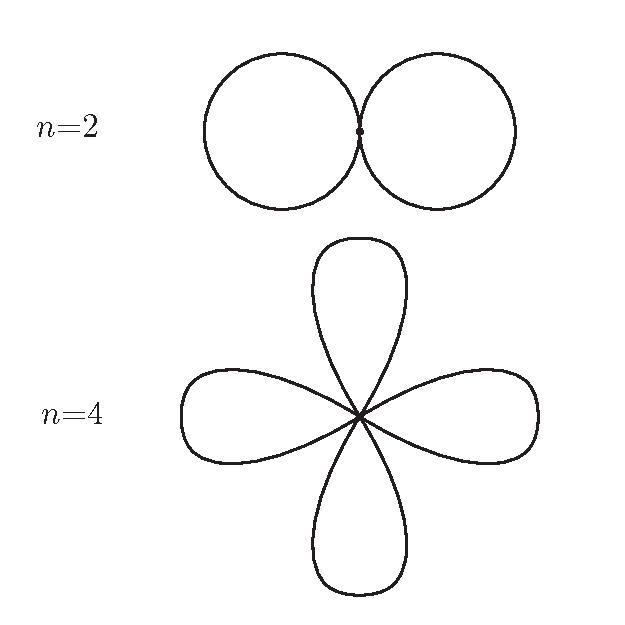
\includegraphics[trim=0cm 0cm 0cm 0cm,clip,scale=0.75]{images/bouquet.pdf}
\end{center}
\vspace{-8mm}
\end{define}
\begin{examples}\textsc{Altri esempi di equivalenze omotopiche.}
	\begin{enumerate}
		\item $\realset^2\setminus\left\{2\text{ punti}\right\}$ ha lo stesso tipo di omotopia di un \textit{bouquet di due circonferenze}: si può ottenere attraverso una composizione (continua) di retrazioni \textit{radiali} e \textit{lineari}.
		\begin{center}
						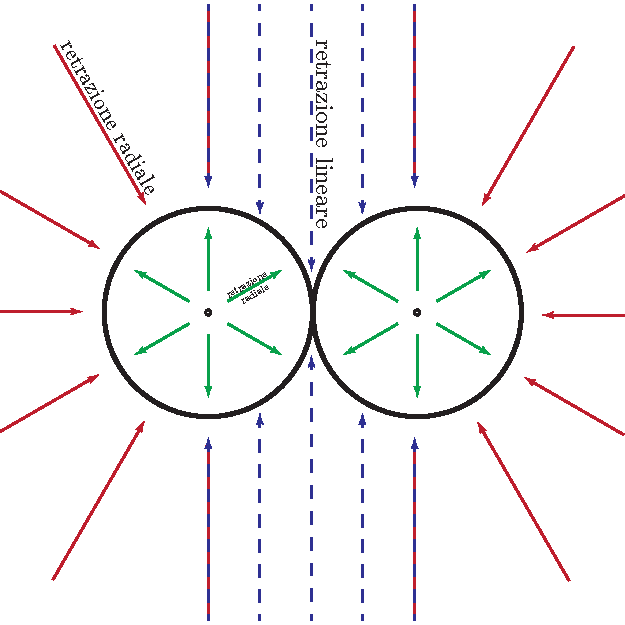
\includegraphics[trim=0cm 0cm 0cm 0cm,clip,scale=0.75]{images/bouquetconstruction.pdf}
		\end{center}	
		\item $\realset^2\setminus\left\{n\text{ punti}\right\}$ ha lo stesso tipo di omotopia di un \textit{bouquet di} $n$ \textit{circonferenze}.
		\item $\realset^3\setminus\left\{1\text{ retta}\right\}$ ha lo stesso tipo di omotopia di $\realset^2\setminus\left\{1\text{ punto}\right\}$ per retrazioni lineari, dunque ha la stessa omotopia di $S^1$ per i ragionamenti precedenti.
		\item Per $\realset^3\setminus\left\{2\text{ rette}\right\}$ dobbiamo distinguere a seconda della relazione fra le due rette.
		\begin{itemize}
			\item Se le rette sono \textbf{disgiunte}, $X$ è sempre omeomorfo a:
			\begin{equation*}
				\realset^3\setminus\left\{\text{asse z}\right\}\setminus\left\{x=y=1\right\}=\widetilde{X}
			\end{equation*}
		Cioè lo spazio $\realset^3$ privato di due rette perpendicolari al piano e distinte.\\
			Considerato ora il piano $Y=\left\{\text{piano xy}\right\}\setminus\left\{\left(0,0\right),\ \left(1,1\right)\right\}$, questo risulta un retratto di deformazione di $\widetilde{X}$ con retrazione:
			\begin{equation*}
				\funztot{r}{\widetilde{X}}{Y}{\left(x,\ y,\ z\right)}{\left(x,\ y, 0\right)}
			\end{equation*}
		Infatti la funzione è sempre ben definita e continua e, considerata la restrizione di $r$ ad $Y$, segue che banalmente che è l'identità di $Y$ in quanto tutti i punti di $Y$ hanno già la forma $\left(x,\ y, 0\right)$. Guardando invece $\widetilde{r}=i\circ r$ con $\incl{i}{Y}{\widetilde{X}}$, un'omotopia con $Id_{\widetilde{X}}$ è:
		\begin{equation*}
			\funz{F}{\widetilde{X}\times I}{\widetilde{X}}\ \colon \mvf{F}{\left(x,\ y,\ z\right)}{t}=\left(x,\ y,\ tz\right)
		\end{equation*}
		Infatti $F$ è banalmente ben definita continua, con $\mvf{F}{\mathbf{x}}{0}=\left(x,\ y,\ 0\right)=\widetilde{r}\left(\mathbf{x}\right)$ e $\mvf{F}{\mathbf{x}}{1}=\left(x,\ y,\ z\right)=Id_{\widetilde{X}}\left(\mathbf{x}\right)$.\\
		Segue che $\widetilde{X}$, e dunque anche $X$ per omeomorfismo, ha la stessa omotopia di $\realset^2\setminus\left\{2\text{ punti}\right\}$ e di un \textit{bouquet di due circonferenze}.
		\item Se le due rette sono \textbf{incidenti}, a meno di omeomorfismi si intersecano nell'origine. Consideriamo dunque $X=\realset^3\left\{r_1\cup r_2\right\}$ e lo spazio $A=S^2\setminus\left\{P_1,\ P_2,\ Q_1,\ Q_2\right\}$. Se prendiamo la retrazione:
		\begin{equation*}
			\funztot{r}{X}{A}{\mathbf{x}}{\frac{\mathbf{x}}{\labs \mathbf{x}\rabs}}.
		\end{equation*}
		e l'omotopia:
		\begin{equation*}
			\widetilde{r}\coloneqq\funztot{ i\circ r}{X}{X}{\mathbf{x}}{\frac{\mathbf{x}}{\labs \mathbf{x}\rabs}}
		\end{equation*}
	Si verifica in modo analogo a come visto nel caso della sfera e dello spazio privato dell'origine (esempio a pagina \ref{retrattosfera}), trattando con una \textit{retrazione radiale} ben definita e la sua omotopia nota, che $A$ è retratto di deformazione di $X$. Segue allora che hanno lo stesso tipo di omotopia.
		\end{itemize}
	\end{enumerate}
	\vspace{-3mm}
\end{examples}

% SVN info for this file
\svnidlong
{$HeadURL$}
{$LastChangedDate$}
{$LastChangedRevision$}
{$LastChangedBy$}

\chapter{Il gruppo fondamentale}
\labelChapter{gruppofonduta}

\begin{introduction}
	‘‘BEEP BOOP INSERIRE CITAZIONE QUA BEEP BOOP.''
	\begin{flushright}
		\textsc{NON UN ROBOT,} UN UMANO IN CARNE ED OSSA BEEP BOOP.
	\end{flushright}
\end{introduction}
%inserire introduzione
%inserire citazione
%controllare gruppo fondamentale banale nomenclatura
\section{Omotopie fra cammini}
\begin{notate}
Se non specificato differentemente, useremo $I$ per indicare l'intervallo $\intv$.
\end{notate}
\begin{define}\textsc{Omotopia di cammini.}\\
	Siano $\funz{\alpha,\ \beta}{I}{X}$ due cammini da $a$ a $b$, cioè con \textit{stessi estremi}. Allora $\alpha,\ \beta$ sono \textbf{cammini omotopi}\index{cammino!omotopo} se $\exists \funz{F}{I \times I}{X}$ tale che:
	\begin{equation}
		\begin{array}{ll}
			\begin{cases}
							\mvf{F}{t}{0}=\alpha\left(t\right)\\
				\mvf{F}{t}{1}=\beta\left(t\right)
			\end{cases}&
		\forall t\in I\ \text{ è omotopia tra } \alpha \text{ e }\beta\\
			\begin{cases}
			\mvf{F}{0}{s}=a\\
			\mvf{F}{1}{s}=b
		\end{cases}&
		\forall s\in I\ \mvf{F}{\bullet}{s} \text{ è sempre un cammino tra } a \text{ e }b
		\end{array}
	\end{equation}
	\begin{center}
	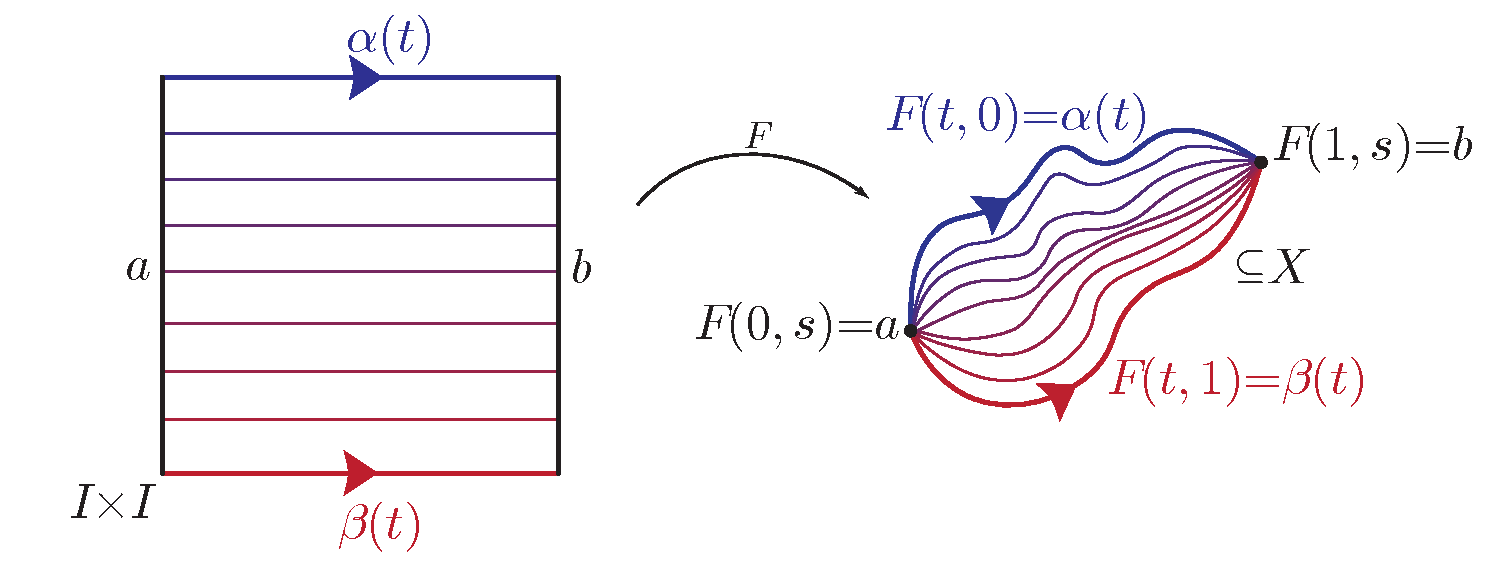
\includegraphics[trim=0cm 0cm 0cm 0cm,clip,scale=0.4]{images/pathhomotopy.pdf}
\end{center}
$F$ è detta \textbf{omotopia di cammini}\index{omotopia!di cammini} o \textbf{omotopia a estremi fissi} \seeonlyindex{omotopia!a estremi fissi}{omotopia!di cammini}.
\end{define}
\begin{define}\textsc{Insieme dei cammini.}\\
	Indichiamo con $\inscam{X}{a}{b}$ l'\textbf{insieme dei cammini}\index{cammino!insieme} in $X$ da $a$ a $b$.
\end{define}
\begin{observe}
	L'omotopia di cammini è una relazione di equivalenza su $\inscam{X}{a}{b}$.
\end{observe}
\begin{demonstration}~{}
		\begin{itemize}
		\item \textsc{Riflessiva}: $\alpha\sim \alpha ?$ Presa $\mvf{F}{t}{s}=\alpha\left(t\right)$, essa è ben definita, continua e:
		\begin{equation*}
			\mvf{F}{t}{0}=\alpha\left(t\right),\ \mvf{F}{t}{1}=\alpha\left(t\right),\ \mvf{F}{0}{s}=\alpha\left(0\right)=a,\ \mvf{F}{1}{s}=\alpha\left(1\right)=b
		\end{equation*}
	Cioè è omotopia di cammini tra $\alpha$ e se stessa.
		\item \textsc{Simmetrica}: Da $\alpha\sim \beta$ sappiamo che esiste $F$ omotopia di cammini per cui:
		\begin{equation*}
			\mvf{F}{t}{0}=\alpha\left(t\right),\ \mvf{F}{t}{1}=\beta\left(t\right),\ \mvf{F}{0}{s}=a,\ \mvf{F}{1}{s}=b
		\end{equation*}
		Per avere $\beta\sim \alpha$, basta prendere $\mvf{\widetilde{F}}{t}{s}=\mvf{F}{t}{1-s}$: essa è ben definita, continua e:
		\begin{gather*}
			\mvf{\widetilde{F}}{t}{0}=\mvf{F}{t}{1}=\beta\left(t\right),\ \mvf{\widetilde{F}}{t}{1}=\mvf{F}{t}{0}=\alpha\left(t\right)\\ \mvf{\widetilde{F}}{0}{s}=\mvf{F}{0}{s}=a,\ \mvf{\widetilde{F}}{1}{s}=\mvf{F}{1}{s}=b
		\end{gather*}
		Cioè è omotopia di cammini tra $\beta$ e $\alpha$.
		\item \textsc{Transitiva}: Da $\alpha\sim \beta$ abbiamo:
	\begin{equation*}
			\begin{array}{ll}
			\begin{cases}
				\mvf{F}{t}{0}=\alpha\left(t\right)\\
				\mvf{F}{t}{1}=\beta\left(t\right)
			\end{cases}&
		\begin{cases}
				\mvf{F}{0}{s}=a\\
				\mvf{F}{1}{s}=b
		\end{cases}
			\end{array}
	\end{equation*}
Mentre da $\beta\sim \gamma$:
	\begin{equation*}
	\begin{array}{ll}
		\begin{cases}
			\mvf{G}{t}{0}=\beta\left(t\right)\\
			\mvf{G}{t}{1}=\gamma\left(t\right)
		\end{cases}&
	\begin{cases}
			\mvf{G}{0}{s}=a\\
			\mvf{G}{1}{s}=b
	\end{cases}
	\end{array}
\end{equation*}
Definita allora la seguente funzione:
\begin{equation*}
	\mvf{H}{t}{s}=\begin{cases}
		\begin{array}{ll}
			\mvf{F}{t}{2s}&\text{se }s\in\left[0,\ \frac{1}{2}\right]\\
			\mvf{G}{t}{2s-1}&\text{se }s\in\left[\frac{1}{2},\ 1\right]
		\end{array}
	\end{cases}
\end{equation*}
Essa è ben definita, continua per il lemma di incollamento e tale per cui:
\begin{gather*}
	\mvf{H}{t}{0}=\mvf{F}{t}{0}=\alpha\left(t\right),\ \mvf{H}{t}{1}=\mvf{G}{t}{1}=\gamma\left(t\right)\\
	\mvf{H}{0}{s}=a,\ \mvf{H}{1}{s}=b
\end{gather*}
		Cioè è omotopia di cammini tra $\alpha$ e $\gamma$.
	\end{itemize}
\vspace{-3mm}
\end{demonstration}
\begin{remember}
Abbiamo già definito due ‘‘operazioni'' fra insiemi di cammini, senza averle necessariamente formalizzate:
\begin{itemize}
\item \textsc{Prodotto di cammini}: $\funztot{\ }{\inscam{X}{a}{b}\times\inscam{X}{b}{c}}{\inscam{X}{a}{c}}{\left(\alpha,\ \beta\right)}{\alpha\ast\beta}$
\item \textsc{Inversione di cammini}: $\funztot{\ }{\inscam{X}{a}{b}}{\inscam{X}{b}{a}}{\alpha}{\overline{\alpha}}$
\end{itemize}
\end{remember}
\begin{observe}
Si ha $\overline{\overline{\alpha}}=\alpha$. Infatti:
\begin{equation*}
	\overline{\alpha}\left(t\right)=\alpha\left(1-t\right)\implies\overline{\overline{\alpha}}\left(t\right)=\overline{\alpha}\left(1-t\right)=\alpha\left(t\right)
\end{equation*}
\vspace{-6mm}
\end{observe}
\begin{lemming}\textsc{Composizioni di omotopie di cammini (Kosniowski, 14.2)\label{compoomotopecammini}}\\
	Dati $\alpha,\ \alpha'\in\inscam{X}{a}{b}$ e $b,\ b'\in\inscam{X}{b}{c}$, parlando in termini di omotopie di cammini:
	\begin{equation}
		\alpha\sim \alpha'\text{ e }\beta\sim \beta'\implies \alpha\ast\beta\sim\alpha'\ast\beta'
	\end{equation}
\vspace{-6mm}
\end{lemming}
\begin{demonstration}
	Esistono $\funz{F,\ G}{I\times I}{X}$ tali che:
	\begin{gather*}
		\begin{array}{ll}
			\mvf{F}{t}{0}=\alpha\left(t\right)&\mvf{F}{0}{s}=a\\
			\mvf{F}{t}{1}=\alpha'\left(t\right)&\mvf{F}{1}{s}=b
		\end{array}
	\forall t,\ s\in I\\
		\begin{array}{ll}
	\mvf{G}{t}{0}=\beta\left(t\right)&\mvf{G}{0}{s}=b\\
	\mvf{G}{t}{1}=\beta'\left(t\right)&\mvf{G}{1}{s}=c
\end{array}	
	\forall t,\ s\in I
	\end{gather*}
Consideriamo $\funz{H}{I\times I}{X}$ data da:
\begin{equation*}
	\mvf{H}{t}{s})\begin{cases}
				\begin{array}{lc}
			\mvf{F}{2t}{s} & \text{se }0\leq t\leq \frac{1}{2}\\
			\mvf{F}{2t-1}{s} & \text{se }\frac{1}{2}\leq t\leq 1	
		\end{array}
	\end{cases}
\end{equation*}
\begin{itemize}
	\item $H$ è ben definita per $t=\frac{1}{2}$
	\item $H$ è continua per il lemma di incollamento, essendo definito sui chiusi $\left[0,\ \frac{1}{2}\right]\times I$ e $\left[\frac{1}{2},\ 1\right]\times I$ è continua su di essi.
\item \parbox[t]{0.25\textwidth}{$\mvf{H}{t}{0}=\left(\alpha\ast\beta\right)\left(t\right)$}\tikzmark{a}
\item \parbox[t]{0.25\textwidth}{$\mvf{H}{t}{1}=\left(\alpha'\ast\beta'\right)\left(t\right)\ $}\tikzmark{b}
\item \parbox[t]{0.25\textwidth}{$\mvf{H}{0}{s}=\mvf{F}{0}{0}=a$}\tikzmark{c}
\item \parbox[t]{0.25\textwidth}{$\mvf{H}{1}{s}=\mvf{G}{1}{0}=c$}\tikzmark{d}
\end{itemize}
\brackitem{a}{b}[$\forall t\in I$ è omotopia]
\brackitem{c}{d}[$\forall s\in I$ ha estremi fissi]
$H$ è l'omotopia a estremi fissi cercata.
\end{demonstration}
\begin{lemming}\textsc{Cambiamento di parametri (Manetti, 11.3)}\label{cambiamentodiparametri}\\
	Sia $\funz{\alpha}{I}{X}$ un cammino e $\funz{\varphi}{I}{I}$ una funzione continua tale che $\varphi\left(0\right)=0$ e $\varphi\left(1\right)=1$. Allora $\alpha\circ \varphi\sim\alpha$.
\end{lemming}
\begin{demonstration}
	Sia $\funz{F}{I\times I}{X}$ data da $\mvf{F}{t}{s}=\alpha\left(s\varphi\left(t\right)+\left(1-s\right)t\right)$.
	\begin{itemize}
		%controllare impaginazione qui
		\item $s\varphi\left(t\right)+\left(1-s\right)t$ è una combinazione lineare che è contenuta in $I\subseteq \realset\ \forall t,\ s\in I$ per convessità dell'intervallo $I$, da cui segue che $F$ è ben definita.
		\item $F$ continua perché composizione di funzioni continue.
		\item \parbox[t]{0.38\textwidth}{$\mvf{F}{t}{0}=\alpha\left(t\right)$}\tikzmark{a}
		\item \parbox[t]{0.38\textwidth}{$\mvf{F}{t}{1}=\alpha\left(\varphi\left(t\right)\right)$}\tikzmark{b}
		\item \parbox[t]{0.38\textwidth}{$\mvf{F}{0}{s}=\alpha\left(0\right)$}\tikzmark{c}
		\item \parbox[t]{0.38\textwidth}{$\mvf{F}{1}{s}=\alpha\left(s+1-s\right)=\alpha\left(1\right)$}\tikzmark{d}
	\end{itemize}
\brackitem{a}{b}[$\forall t\in I$ è omotopia]
\brackitem{c}{d}[$\forall s\in I$ ha estremi fissi]
$H$ è l'omotopia a estremi fissi cercata tra $\alpha$ e $\alpha\circ\varphi$.
\end{demonstration}
\begin{define}\textsc{Cammino costante.}\\
	Il \textbf{cammino costante} $C_a$\index{cammino!costante} nel punto $a$ è un cammino che non si sposta mai da esso, cioè è descritto da una funzione costante nel punto:
	\begin{equation}
		\funztot{C_a}{I}{X}{t}{a}
	\end{equation}
\vspace{-6mm}
\end{define}
\begin{proposition}\textsc{(Manetti, 11.4 e 11.6)\label{propcammini}}\\
	Sia $X$ spazio topologico e si considerino i cammini:
	\begin{equation*}
	\alpha\in\inscam{X}{a}{b}\quad\beta\in\inscam{X}{b}{c}\quad\gamma\in\inscam{X}{c}{d}
	\end{equation*}
Valgono le seguenti proprietà:
\begin{enumerate}
	\item \textsc{Associatività}: $\left(\alpha\ast\beta\right)\ast \gamma \sim \alpha\ast\left(\beta\ast\gamma\right)$.
	\item \textsc{Rapporto coi cammini costanti}: $C_a\ast \alpha \sim \alpha \sim \alpha \ast C_b$. 
	\item \textsc{Inverso}: $\alpha\ast\overline{\alpha}\sim C_a$ e $\overline{\alpha}\ast\alpha\sim C_a$.
\end{enumerate}
\end{proposition}
\begin{demonstration}~{}
\begin{enumerate}[label=\Roman*]
	\item Scriviamo i due cammini:
	\begin{gather*}
\left(\left(\alpha\ast\beta\right)\ast\gamma\right)\left(t\right)=\begin{cases}
	\begin{array}{ll}
		\alpha\left(4t\right)&t\in\left[0,\ \frac{1}{4}\right]\\
		\beta\left(4t-1\right)&t\in\left[\frac{1}{4},\ \frac{1}{2}\right]\\
		\gamma\left(2t-1\right)&t\in\left[\frac{1}{2},\ 1\right]
	\end{array}
\end{cases}\\
\left(\left(\alpha\ast\left(\beta\gamma\right)\right)\right)\left(t\right)=\begin{cases}
\begin{array}{ll}
	\alpha\left(2t\right)&t\in\left[0,\ \frac{1}{2}\right]\\
	\beta\left(4t-2\right)&t\in\left[\frac{1}{2},\ \frac{3}{4}\right]\\
	\gamma\left(2t-3\right)&t\in\left[\frac{3}{4},\ 1\right]
\end{array}
\end{cases}
	\end{gather*}
I due cammini differiscono per una \textit{riparametrizzazione} $\funz{\oldphi}{I}{I}$ di $\alpha\ast\left(\beta\ast\gamma\right)$ definita in questo modo:
\begin{gather*}
	\begin{cases}
		\begin{array}{l}
			2s=4t\\
			4s-2=4t-2\\
			4s-3=4t-1
		\end{array}
\implies
\begin{cases}
\begin{array}{ll}
	s=2t&t\in\left[0,\ \frac{1}{2}\right]\\
	s=t+\frac{1}{4}&t\in\left[\frac{1}{4},\ \frac{1}{2}\right]\\
	s=\frac{t}{2}+\frac{1}{2}&t\in\left[\frac{1}{2},\ 1\right]
\end{array}
		\end{cases}
	\end{cases}\\
\oldphi\left(t\right)=	\begin{cases}
\begin{array}{ll}
	2t&t\in\left[0,\ \frac{1}{2}\right]\\
	t+\frac{1}{4}&t\in\left[\frac{1}{4},\ \frac{1}{2}\right]\\
	\frac{t}{2}+\frac{1}{2}&t\in\left[\frac{1}{2},\ 1\right]
\end{array}
		\end{cases}
\end{gather*}
\begin{itemize}
	\item $\oldphi$ è ben definita e continua per lemma di incollamento.
	\item $\oldphi\left(0\right)=0$ e $\oldphi\left(1\right)=1$.
	\item $\left(\left(\alpha\ast\left(\beta\ast\gamma\right)\right)\right)\left(\oldphi\left(t\right)\right)=\left(\left(\alpha\ast\beta\right)\ast\gamma\right)\left(t\right)$.
\end{itemize}
Per il lemma del cambiamento di parametro i due cammini sono omotopi.
\item Scriviamo i due cammini:
\begin{gather*}
	\left(C_a\ast \alpha\right)\left(t\right)=\begin{cases}
		\begin{array}{ll}
			a&t\in\left[0,\ \frac{1}{2}\right]\\
			\alpha\left(2t-1\right)&t\in\left[\frac{1}{2},\ 1\right]
		\end{array}
	\end{cases}\\
	\left(\alpha\ast C_b\right)\left(t\right)=\begin{cases}
		\begin{array}{ll}
			\alpha\left(2t\right)&t\in\left[0,\ \frac{1}{2}\right]\\
			b&t\in\left[\frac{1}{2},\ 1\right]
		\end{array}
	\end{cases}
\end{gather*}
I due cammini differiscono per delle \textit{riparametrizzazioni} di $\alpha$ $\funz{\oldphi}{I}{I}$ e $\funz{\psi}{I}{I}$ definite così:
\begin{equation*}
	\oldphi\left(t\right)=
	\begin{cases}
		\begin{array}{ll}
			0&t\in\left[0,\ \frac{1}{2}\right]\\
			2t-1&t\in\left[\frac{1}{2},\ 1\right]
		\end{array}
	\end{cases}
\qquad	\psi\left(t\right)=
\begin{cases}
	\begin{array}{ll}
		2t&t\in\left[0,\ \frac{1}{2}\right]\\
		1&t\in\left[\frac{1}{2},\ 1\right]
	\end{array}
\end{cases}
\end{equation*}
\begin{itemize}
	\item $\oldphi$ e $\psi$ son ben definite e continue per lemma di incollamento.
	\item $\oldphi\left(0\right)=0,\ \psi\left(0\right)=0$ e $\oldphi\left(1\right)=1,\psi\left(1\right)=1 $.
	\item $\left(C_a\ast \alpha\right)\left(t\right)=\alpha\left(\oldphi\left(t\right)\right)$ e $\left(\alpha\ast C_b\right)\left(t\right)=\alpha\left(\psi\left(t\right)\right)$.
\end{itemize}
Per il lemma del cambiamento di parametro i due cammini sono entrambi omotopi a $\alpha$, si hanno quindi le equivalenze omotopiche cercate.
\item È sufficiente dimostrare che $\alpha\ast\overline{\alpha}\sim C_a$. Possiamo immaginare di rappresentare tutte le parametrizzazioni di cammini definiti da un omotopia sul piano $I\times I$, con $t$ sulle ascisse e $s$ sulle ordinate.\\
In questo modo i punti $a$ di inizio e $b$ di fine sono rappresentati dai segmenti verticali in $t=0$ e in $t=1$, mentre i cammini $\alpha$ di inizio e $\beta$ fine sono segmenti orizzontali in $s=0$ e $s=1$. Dunque, all'interno di $I\times I$ possiamo  trovare (fissato $s$) tutti i cammini $\mvf{F}{\bullet}{s}$ di estremi $a$ e $b$ compresi tra i cammini $\alpha$ e $\beta$: essi sono rappresentati da segmenti orizzontali.\\
\begin{minipage}{.62\linewidth}
Nel nostro caso, possiamo considerare il punto $a$ di inizio e il punto $b$ di fine del cammino $\alpha$. Nei due cammini ‘‘esterni'' o il cammino non si sposta mai da $a$ ($C_a$), oppure percorre tutto il cammino $\alpha$ fino a $b$ (che è raggiunto per $t=\frac{1}{2}$) e torna poi indietro per lo \textit{stesso cammino} ($\alpha\ast\overline{\alpha}$). Tuttavia, dobbiamo considerare anche cammini che percorrono $\alpha$ fino ad un punto $c$ \textit{intermedio} fra $a$ e $b$, stanno fermi in $c$ per poi tornare indietro. Definiamo la seguente omotopia:
\end{minipage}
\begin{minipage}{.37\linewidth}
	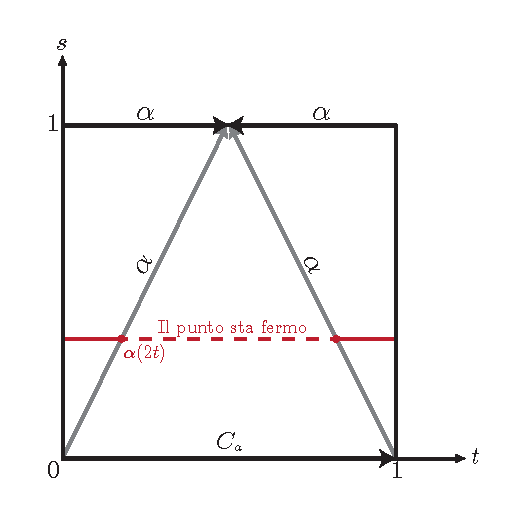
\includegraphics[trim=0cm 0cm 0cm 0cm,clip,scale=0.6]{images/camminoinverso.pdf}
\end{minipage}
\begin{equation}
	\mvf{F}{t}{s}=\begin{cases}
		\begin{array}{ll}
			\alpha\left(2t\right)&\text{se }0\leq t\leq \frac{s}{2}\\
			\alpha\left(s\right)&\text{se }\frac{s}{2}\leq t\leq 1-\frac{s}{2}\\
			\alpha\left(2-2t\right)&\text{se }1-\frac{s}{2}\leq t\leq 1
		\end{array}
	\end{cases}
\end{equation}
Verifichiamo che lo sia:
\begin{itemize}
\item $F$ è ben definita grazie alla ben definizione di $\alpha$: tutti i valori di $F$ risultano interni ad $X$.
\item $F$ è continua per il lemma di incollamento.
\item $\mvf{F}{t}{0}=\alpha\left(0\right)=C_a\left(t\right),\ \mvf{F}{t}{1}=\alpha\ast\overline{\alpha}\left(t\right)$ e $\mvf{F}{0}{s}=a=\mvf{F}{1}{s}$.
\end{itemize}
In questo modo teniamo conto della possibilità del cammino di ‘‘fermarsi'' per un certo tempo in un particolare punto $\alpha\left(s\right)$. 
\end{enumerate}
\vspace{-3mm}
\end{demonstration}
\section{Gruppo fondamentale}
\begin{define}\textsc{Laccio.}\\
	Sia $X$ uno spazio topologico e fissiamo un punto $x_0\in X$. I \textbf{lacci}\index{laccio} o \textbf{cappi}\seeonlyindex{cappio}{laccio} sono i cammini chiusi in $X$, cioè tutti i cammini il cui punto iniziale e finale coincidono. Il loro insieme si denota dunque come $\inscam{X}{x_0}{x_0}$.
\end{define}
\begin{observe}
	Possiamo notare come $\forall\alpha,\ \beta\in\inscam{X}{x_0}{x_0}$ si ha:
	\begin{equation*}
		\alpha\ast\beta\in\inscam{X}{x_0}{x_0}\qquad \overline{\alpha}\in\inscam{X}{x_0}{x_0}
	\end{equation*}
Allora, se quozientiamo l'insieme dei lacci rispetto alla relazione di equivalenza data dall'omotopia di cammini, esso possiede una struttura di \textit{gruppo}:
\begin{equation}
	\begin{array}{cc}
	\gruf{X}{x_0}=&\frac{\inscam{X}{x_0}{x_0}}{\sim}
	\end{array}	
\end{equation}
Preso un laccio $\alpha$, indichiamo la sua classe di equivalenza in $\gruf{X}{x_0}$ con $\left[\alpha\right]$. Allora:
\begin{itemize}
	\item Il prodotto di cammini dà un operazione ben definita su $\gruf{X}{x_0}$ grazie al lemma \ref{compoomotopecammini} (Kosniowski, 14.2):
	\begin{equation}
		\left[\alpha\right]\cdot\left[\beta\right]=\left[\alpha\ast\beta\right]
	\end{equation}
\item L'operazione appena definita è associativa per il primo punto della proposizione \ref{propcammini} (Manetti, 11.4 e 11.6).
\item $\left[C_{x_0}\right]$ è l'elemento neutro, sempre per la proposizione \ref{propcammini} (Manetti, 11.4 e 11.6):
\begin{equation}
	\left[C_{x_0}\right]\cdot\left[\alpha\right]=\left[\alpha\right]=\left[\alpha\right]\cdot\left[C_{x_0}\right]
\end{equation} 
\item $\left[\overline{\alpha}\right]$ è l'inverso di $\left[\alpha\right]$, cioè $\left[\alpha\right]^{-1}\coloneqq\left[\overline{\alpha}\right]$, per la proposizione \ref{propcammini} (Manetti, 11.4 e 11.6):
\begin{equation}
\left[\overline{\alpha}\right]\cdot\left[\alpha\right]=\left[C_{x_0}\right]=\left[\alpha\right]\cdot\left[\overline{\alpha}\right]
\end{equation}
\end{itemize}
\vspace{-6mm}
\end{observe}
\begin{attention}
	La proposizione \ref{propcammini} (Manetti, 11.4 e 11.6) ci garantisce che la composizione di cammini omotopi è omotopa ($\left(\alpha\ast\beta\right)\ast \gamma \sim \alpha\ast\left(\beta\ast\gamma\right)$), dunque possiamo parlare della \textit{classe} $\left[\alpha\ast\beta\ast\gamma\right]$. Tuttavia, al di fuori del quoziente non ha senso $\alpha\ast\beta\ast\gamma$!\\
	L'ordine con cui congiungiamo i cammini dà luogo a due cammini certamente omotopi, \textit{ma non uguali}, dato che la parametrizzazione varia\footnote{Questo si vede chiaramente nella dimostrazione della proposizione.}.
\end{attention}
\begin{define}\textsc{Gruppo fondamentale.}\\
	Dato uno spazio topologico $X$ e fissato un punto (detto \textbf{punto base}\index{punto!base}) $x_0$, il \textbf{gruppo fondamentale}\index{gruppo!fondamentale} con punto base $x_0$ è il gruppo $\gruf{X}{x_0}$ definito nell'osservazione precedente.\\
	Si chiama anche \textbf{primo gruppo fondamentale}\index{gruppo!fondamentale!primo} o \textbf{gruppo di Poincaré}\seeonlyindex{gruppo!di Poicaré}{gruppo!fondamentale}.
\end{define}
\subsection{Dipendenza dal punto base}
\begin{theorema}\label{dipendenzaptobasegruf}
	Il gruppo fondamentale dipende \textit{solo} dalla componente \textit{\textbf{c.p.a.}} contente il punto base $x$.\\
	In altre parole, se $x,\ y\in X$ appartengono alla stessa componente \textbf{c.p.a.}, preso un arco $\gamma$ da $x$ a $y$ e costruito:
	\begin{equation}
		\funztot{\gamma_{\#}}{\gruf{X}{x}}{\gruf{X}{y}}{\left[\alpha\right]}{\left[\overline{\gamma}\ast\alpha\ast\gamma\right]}
	\end{equation}
	È ben definito ed è un \textit{isomorfismo} di gruppi, cioè:
	\begin{equation}
		\gruf{X}{x}\cong\gruf{X}{y}
	\end{equation}
\vspace{-6mm}
\end{theorema}
\begin{remember}
	Una funzione fra due gruppi $\funz{f}{\left(G,\ \cdot_G\right)}{\left(H,\ \cdot_H\right)}$ è un \textbf{omomorfismo di gruppi}\index{omomorfismo di gruppi} se:
	\begin{gather*}
		f\left(a\cdot_G b\right)=f\left(a\right)\cdot_H f\left(b\right)\quad \forall a,\ b\in G
	\end{gather*}
	Se $f$ è \textit{biettiva}, allora parliamo di \textbf{isomorfismo di gruppi}\index{isomorfismo di gruppi}.
\end{remember}
\begin{demonstration}~{}
	\begin{itemize}
		\item $\gamma_{\#}$ è ben definito in quanto la classe $\left[\overline{\gamma}\ast\alpha\ast\gamma\right]$ è ben definita per la composizione dei cammini ed è la classe di equivalenza di un cappio di $y$ ($\overline{\gamma}$ parte da $y$ e raggiunge $x$, con $\alpha$ compie un cammino chiuso in $x$ per tornare al punto di partenza $y$).
		\item $\gamma_{\#}$ è un omomorfismo di gruppi:
		\begin{equation*}
			\begin{array}{lll}
				\gamma_{\#}\left(\left[\alpha\right]\ast\left[\beta\right]\right)&=\gamma_{\#}\left(\left[\alpha\ast\beta\right]\right)=\left[\overline{\gamma}\ast\alpha\ast\beta\ast\gamma\right]=\left[\overline{\gamma}\ast\alpha\ast C_x\ast\beta\ast\gamma\right]\\
				&=\left[\overline{\gamma}\ast\alpha\ast \gamma\ast\overline{\gamma}\ast\beta\ast\gamma\right]=\left[\overline{\gamma}\ast\alpha\ast\gamma\right]\cdot\left[\overline{\gamma}\ast\beta\ast\gamma\right]=\gamma_{\#}\left(\left[\alpha\right]\right)\cdot \gamma_{\#}\left(\left[\beta\right]\right)
			\end{array}
		\end{equation*}
	Infatti, anche l'elemento neutro viene mappato all'elemento neutro del codominio:
	\begin{equation*}
		\gamma_{\#}\left(\left[C_x\right]\right)=\left[\overline{\gamma}\ast C_x\ast\gamma\right]=\left[\overline{\gamma}\ast\gamma\right]=\left[C_y\right]
	\end{equation*}
	\item Possiamo associare in modo analogo al cammino $\overline{\gamma}$ il cammino:
	\begin{equation*}
		\funztot{\overline{\gamma}_{\#}}{\gruf{X}{y}}{\gruf{X}{x}}{\left[\alpha\right]}{\left[\gamma\ast\alpha\ast\overline{\gamma}\right]}
	\end{equation*}
In modo assolutamente analogo a come visto sopra, si vede che è un omeomorfismo; verifichiamo ora che $\gamma_{\#}$ e $\overline{\gamma}_{\#}$ siano l'uno l'inverso dell'altro:
\begin{gather*}
	\overline{\gamma}_{\#}\left(\gamma_{\#}\left(\left[\alpha\right]\right)\right)=\overline{\gamma}_{\#}\left(\left[\overline{\gamma}\ast\alpha\ast\gamma\right]\right)=\left[\gamma\ast\overline{\gamma}\ast\alpha\ast\gamma\ast\overline{\gamma}\right]=\left[C_x\ast\alpha\ast C_x\right]=\left[\alpha\right]\\
	\gamma_{\#}\left(\overline{\gamma}\left(\left[\alpha\right]\right)\right)=
	\gamma_{\#}\left(\left[\gamma\ast\alpha\ast\overline{\gamma}\right]\right)=\left[\overline{\gamma}\ast\gamma\ast\alpha\ast\overline{\gamma}\ast\gamma\right]=\left[C_y\ast\alpha\ast C_y\right]=\left[\alpha\right]
\end{gather*}
Segue che allora $\gamma_{\#}$ è biettiva.
\end{itemize}
\vspace{-3mm}
\end{demonstration}
\begin{observes}~{}
	\begin{itemize}
		\item Se due punto $x_1$ e $x_2$ stanno in componenti connesse per archi diverse, \textit{non} c'è alcuna relazione tra $\gruf{X}{x_1}$ e $\gruf{X}{x_2}$.
		\item Se $X$ è \textbf{c.p.a.}, il suo gruppo fondamentale è \textit{unico} a meno di isomorfismo.
	\end{itemize}
\vspace{-3mm}
\end{observes}
\begin{example}
	Sia $Y\subseteq \realset^n$ un sottospazio convesso e $y_0\in Y$.
	Allora $\gruf{Y}{y_0}=0$ è \textbf{banale}; in particolare, allora $\gruf{\realset^n}{y_0}$ è banale per ogni $n$.
\end{example}
\begin{demonstration}
	Sia $\left[\alpha\right]\in\gruf{Y}{y_0}$. Vogliamo mostrare che $\left[\alpha\right]=\left[C_{y_0}\right]$, cioè che $\alpha\sim C_{y_0}$.\\
	Consideriamo $\funz{F}{X\times I}{Y}$ tale che:
	\begin{equation*}
		\mvf{F}{t}{s}=s\left(\alpha\left(t\right)\right)+\left(1-s\right)y_0
	\end{equation*}
\begin{itemize}
	\item $F$ risulta ben definita: è una combinazione convessa al variare di $s\in\intv$ tra $\alpha\left(t\right)\in Y$ (per $t$ fissato) e $y_0\in Y$.
	\item $F$ è continua perché composizione di applicazioni continue.
	\item $\mvf{F}{t}{0}=y_0=C_{y_0}\left(t\right),\ \mvf{F}{t}{1}=\alpha\left(t\right)$.
	\item $\mvf{F}{0}{s}=s\alpha\left(0\right)+\left(1-s\right)y_0=sy_0+\left(1-s\right)y_0=y_0,\ \mvf{F}{1}{s}=s\alpha\left(1\right)+\left(1-s\right)y_0=sy_0+\left(1-s\right)y_0=y_0$.
\end{itemize}
Segue che $F$ è un omotopia tra $C_{y_0}$ e $\alpha$, dunque segue la tesi.
\end{demonstration}
\begin{define}\textsc{Spazio semplicemente connesso.}\\
	Uno spazio topologico $X$ è \textbf{semplicemente connesso}\index{semplicemente connesso} se è \textbf{c.p.a.} e ha gruppo fondamentale \textbf{banale}.
\end{define}
\begin{examples}~{}
	\begin{itemize}
		\item $\realset^n$ è semplicemente connesso.
		\item Ogni convesso di $\realset^n$ è semplicemente connesso.
	\end{itemize}
\vspace{-3mm}
\end{examples}
\subsection{Mappe continue e omomorfismo di gruppi}
\begin{notate}
	$\funz{f}{\left(X,\ x_0\right)}{\left(Y,\ y_0\right)}$ è una funzione continua $\funz{f}{X}{Y}$ tale che $f\left(x_0\right)=y_0$.
\end{notate}
\begin{observe}
Consideriamo $\funz{f}{X}{Y}$ continua e due cammini $\alpha$ in $X$ da $a$ a $b$ e $\beta$ in $X$ da $b$ a $c$.
\begin{center}
	\begin{tikzcd}
		I \arrow[r, "\alpha"] \arrow[rr, "f\circ \alpha"', bend right] & X \arrow[r, "f"] & Y
	\end{tikzcd}
\begin{tikzcd}
	I \arrow[r, "\beta"] \arrow[rr, "f\circ \beta"', bend right] & X \arrow[r, "f"] & Y
\end{tikzcd}
\end{center}
Si ha che:
\begin{enumerate}
\item $f\circ \left(\alpha\ast\beta\right)=\left(f\circ\alpha\right)\ast\left(f\circ \beta\right)$.
\item $f\circ\overline{\alpha}=\overline{f\circ\alpha}$.
\item Se $\alpha\sim\alpha'$, allora $f\circ\alpha\sim f\circ\alpha'$.
\end{enumerate}
\vspace{-3mm}
\end{observe}
\begin{proposition}
	Dati $X,\ Y$ spazi topologici, due punti $x_0\in X,\ y_0\in Y$ e una funzione $\funz{f}{\left(X,\ x_0\right)}{\left(Y,\ y_0\right)}$ continua, si può definire associare un omomorfismo tra i corrispettivi gruppi fondamentali:
	\begin{equation}
		\funztot{f_{\ast}}{\gruf{X}{x_0}}{\gruf{Y}{y_0}}{\left[\alpha\right]}{\left[f\circ\alpha\right]}
	\end{equation}
\vspace{-6mm}
\end{proposition}
\begin{demonstration}~{}
	\begin{itemize}
		\item $f_{\ast}$ è ben definita: infatti, $f\circ\alpha\in\inscam{Y}{y_0}{y_0}$ e se $\left[a\right]=\left[a'\right]$, $\alpha\sim\alpha'$. Per il punto 3 dell'osservazione precedente, si ha $f\circ \alpha\sim f\circ\alpha'$, cioè $\left[f\circ \alpha\right]=\left[f\circ\alpha'\right]$.
		\item $f_{\ast}$ è un omeomorfismo di gruppi: infatti, presi $\left[\alpha\right],\ \left[\beta\right]\in\gruf{X}{x_0}$, si ha:
		\begin{align*}
			f_{\ast}\left(\left[\alpha\right]\cdot\left[\beta\right]\right)&=f_{\ast}\left(\left[\alpha\ast\beta\right]\right)=\left[f\circ\left(\alpha\ast\beta\right)\right]\stackrel{1}{=}\left[\left(f\circ\alpha\right)\ast\left(f\circ\beta\right)\right]=\left[f\circ\alpha\right]\cdot\left[f\circ\beta\right]=\\&=f_{\ast}\left(\left[\alpha\right]\right)\cdot f_{\ast}\left(\left[\beta\right]\right)
		\end{align*}
	Inoltre: $f_{\ast}\left(\left[C_{x_0}\right]\right)=\left[f\circ C_{x_0}\right]=\left[C_{y_0}\right]$.
	\end{itemize}
\vspace{-3mm}
\end{demonstration}
\section{Digressione: Categorie}
\begin{define}\textsc{Categoria.}\\
	Una \textbf{categoria}\index{categoria} $\cat$ consiste di:
	\begin{itemize}
		\item Una \textbf{classe}\index{classe} $\mathrm{Ob}\left(\cat\right)$, i cui elementi sono datti \textbf{oggetti}\index{oggetto} di $\cat$.
		\item Per ogni \textit{coppia} di oggetti $X$ e $Y$ di $\cat$ una classe $\homo{\cat}{X}{Y}$, i cui elementi sono detti \textbf{morfismi}\index{morfismo} da $X$ a $Y$.
		\item Per ogni \textit{terna} di oggetti $X,\ Y,\ Z$ un'operazione binaria detta \textbf{composizione}\index{composizione} di morfismi:
		\begin{equation}
			\funztot{\ }{\homo{\cat}{X}{Y}\times \homo{\cat}{Y}{Z}}{\homo{\cat}{X}{Z}}{\left(f,\ g\right)}{g\circ f}
		\end{equation}
	\end{itemize}
Tali che questi oggetti soddisfino i seguenti assiomi:
\begin{enumerate}
	\item \textsc{Associatività}: Per ogni $f\in\homo{\cat}{X}{Y},\ g\in\homo{\cat}{Y}{Z},\ h\in\homo{\cat}{Z}{W}$ si ha:
	\begin{equation}
		h\circ\left(g\circ f\right)=\left(h\circ g\right)\circ f\text{ in }\homo{\cat}{X}{W}
	\end{equation}
	\item \textsc{Identità}: Per ogni oggetto $X$ esiste un \textbf{morfismo identità}\index{morfismo!identità} $Id_{X}\in\homo{\cat}{X}{X}$ tale che:
	\begin{equation}
		\begin{array}{cc}
			f\circ Id_X=f&Id_X\circ g=g\\
			\forall f\in\homo{\cat}{X}{Y}&\forall g\in\homo{\cat}{Z}{X}
		\end{array}
	\end{equation}
Si dimostra che $Id_X$ è unico per ogni oggetto $X$.
\end{enumerate}
\vspace{-3mm}
\end{define}
\begin{define}\textsc{Isomorfismo.}\\
	Un morfismo $f\in\homo{\cat}{X}{Y}$ si dice \textbf{isomorfismo} se:
	\begin{equation}
		 \exists g\in \homo{\cat}{Y}{X} \text{ tale che } g\circ f=Id_X\qquad f\circ g=Id_Y
	\end{equation}
In tal caso $g$ è unico e si pone $g=f^{-1}$.\\
Inoltre, due oggetti $X$ e $Y$ sono \textbf{isomorfi} se $\exists f\in \homo{\cat}{X}{Y}$ isomorfismo.
\end{define}
\begin{examples}\textsc{Esempi di categorie}
	\begin{itemize}	
\item \begin{tabular*}{6cm}[t]{p{1cm}>{\bfseries}ll}
$\nicecat{SET}$ & Oggetti:  & insiemi. \\
& Morfismi: & applicazioni tra insiemi.
\end{tabular*}
\item \begin{tabular*}{6cm}[t]{p{1cm}>{\bfseries}ll}
$\nicecat{GR}$ ~\footnote{Indicata anche con \nicecat{GRP}.}&Oggetti:  & gruppi. \\
&Morfismi: & omomorfismi di gruppi.
\end{tabular*} 
\item \begin{tabular*}{6cm}[t]{l>{\bfseries}ll}
$\nicecat{VECT}_{\kamp}$ su campo $\kamp$ &Oggetti:  & spazi vettoriali su $\kamp$. \\
&Morfismi: & applicazioni lineari.
\end{tabular*} 
\item \begin{tabular*}{6cm}[t]{p{1cm}>{\bfseries}ll}
$\nicecat{TOP}$ & Oggetti:  & spazi topologici. \\
&Morfismi: & applicazioni continue.
\end{tabular*}
\item \begin{tabular*}{6cm}[t]{p{1cm}>{\bfseries}ll}
$\nicecat{TOP*}$ & Oggetti:  & spazi topologici con punto base $(X,\ x_0)$. \\
&Morfismi: & applicazione continue $\funz{f}{(X,\ x_0)}{(Y,\ y_0)}$.
\end{tabular*}
\item \begin{tabular*}{6cm}[t]{p{1cm}>{\bfseries}ll}
$\nicecat{KTOP}$ & Oggetti:  & spazi topologici. \\
&Morfismi: & classi di omotopia di funzioni continue da $X$ a $Y$.\footnote{La composizione in $\nicecat{KTOP}$ è garantita dalla composizione di omotopie, cioè dal lemma \ref{compomotop} (Manetti 10.13).}
\end{tabular*} 
\item Preso uno spazio topologico $X$, si può considerare la categoria $\cat$ seguente: \begin{tabular*}{6cm}[t]{>{\bfseries}ll}
Oggetti:  & aperti di $X$. \\
Morfismi: & inclusioni.
\end{tabular*}\\
Nello specifico, se $U,\ V\subseteq X$ aperti, allora:
\begin{equation*}
	\homo{\cat}{U}{V}=\begin{cases}
		\begin{array}{ll}
			\emptyset & \text{se } U\nsubseteq V\\
			\left\{i\right\} & \text{ se} U\stackrel{i}{\hookrightarrow} V
		\end{array}
	\end{cases}
\end{equation*}
\end{itemize}
\vspace{-6mm}
\end{examples}
\begin{attention}
	Come si evince dall'esempio 6, i morfismi delle categorie possono anche \textit{non} essere funzioni!
\end{attention}
\subsection{Funtori}
\begin{define}\textsc{Funtore.}\\
Siano $\mathcal{A},\ \mathcal{B}$ due categorie. Un \textbf{funtore}\index{funtore} $\funz{F}{\mathcal{A}}{\mathcal{B}}$ consiste di due funzioni:
\begin{enumerate}
	\item Una \textit{funzione sugli oggetti} $\funztot{F}{\mathrm{Ob}\left(\mathcal{A}\right)}{\mathrm{Ob}\left(\mathcal{B}\right)}{x}{F\left(x\right)}$.
	\item Una \textit{funzione sui morfismi} che, a seconda della sua costruzione, definisce due tipi di funtori:
	\begin{itemize}
		\item Parliamo di \textbf{funtore covariante}\index{funtore!covariante}\footnote{In letteratura, il \textit{funtore covariante} spesso viene indicato anche solo come \textit{funtore}.} se, per ogni coppia di oggetti $X,\ Y$ in $\mathcal{A}$, si ha un'applicazione:
		\begin{equation}
			\funztot{F}{\homo{\mathcal{A}}{X}{Y}}{\homo{\mathcal{A}}{F\left(X\right)}{F\left(Y\right)}}{f}{F\left(f\right)}
		\end{equation}
	Che preserva i morfismi identità e la composizione:
	\begin{itemize}
		\item \textsc{Identità}: $\forall X\in \mathrm{Ob}\left(\mathcal{A}\right)$
		\begin{equation}
			\quad F\left(Id_X\right)=Id_{F\left(X\right)}
		\end{equation}
		\item \textsc{Composizione}: $\forall f\in\homo{\mathcal{A}}{X}{Y},\ g\in\homo{\mathcal{A}}{Y}{Z}$
		\begin{equation}
			F\left(g\circ f\right)=F\left(g\right)\circ F\left(f\right)
		\end{equation}
	\end{itemize}
	\begin{center}
\begin{tikzcd}
	X \arrow[rr, "f"] \arrow[rd, "g\circ f"'] &   & Z \arrow[ld, "g"] \arrow[rr, bend left, shift right=10, squiggly] &  & F\left(X\right) \arrow[rr, "F\left(f\right)"] \arrow[rd, "F\left(g\circ f\right)"'] &                 & F\left(Y\right) \arrow[ld, "F\left(g\right)"] \\
	& Z &                                                              &  &                                                                                     & F\left(Z\right) &                                              
\end{tikzcd}
\end{center}
\item Parliamo di \textbf{funtore controvariante}\index{funtore!controvariante} se, per ogni coppia di oggetti $X,\ Y$ in $\mathcal{A}$, si ha un'applicazione:
\begin{equation}
	\funztot{F}{\homo{\mathcal{A}}{X}{Y}}{\homo{\mathcal{A}}{F\left(Y\right)}{F\left(X\right)}}{f}{F\left(f\right)}
\end{equation}
Che preserva i morfismi identità, mentre inverte la direzione della composizione:
\begin{itemize}
	\item \textsc{Identità}: $\forall X\in \mathrm{Ob}\left(\mathcal{A}\right)$:
	\begin{equation}
		\quad F\left(Id_X\right)=Id_{F\left(X\right)}
		\end{equation}
		\item \textsc{Composizione}: $\forall f\in\homo{\mathcal{A}}{X}{Y},\ g\in\homo{\mathcal{A}}{Y}{Z}$:
		\begin{equation}
			F\left(g\circ f\right)=F\left(f\right)\circ F\left(g\right)
		\end{equation}
	\begin{center}
			\begin{tikzcd}
			X \arrow[rr, "f"] \arrow[rd, "g\circ f"'] &   & Z \arrow[ld, "g"] \arrow[squiggly, rr, bend left, shift right=10] &  & F\left(X\right) &                                                                                     & F\left(Y\right) \arrow[ll, "F\left(f\right)"'] \\
			& Z &                                         &  &                 & F\left(Z\right) \arrow[lu, "F\left(g\circ f\right)"] \arrow[ru, "F\left(g\right)"'] &                                               
		\end{tikzcd}
	\end{center}
	\end{itemize}
	\end{itemize}
\end{enumerate}
\end{define}
\begin{observes}
	Un funtore porta:
	\begin{itemize}
		\item Isomorfismi in isomorfismi,
		\item Oggetti isomorfi in oggetti isomorfi.
	\end{itemize}
\vspace{-3mm}
\end{observes}
\begin{demonstration}
	Se $f\in \homo{\mathcal{A}}{X}{Y}$ è isomorfismo in $\mathcal{A}$, $\exists g\in\homo{\mathcal{A}}{Y}{X}$ tale che $g=f^{-1}$, cioè $g\circ f=Id_X,\ f\circ g=Id_Y$. Ma allora, se $F$ è covariante:
	\begin{gather*}
		F\left(g\right)\circ F\left(f\right)=F\left(g\circ f\right)=F\left(Id_X\right)=Id_{F\left(X\right)}\\
		F\left(f\right)\circ F\left(g\right)=F\left(f\circ g\right)=F\left(Id_Y\right)=Id_{F\left(Y\right)}
	\end{gather*}
$F\left(f\right)\in\homo{\mathcal{A}}{F\left(X\right)}{F\left(Y\right)}$ è isomorfismo con inversa $F\left(g\right)\in\homo{\mathcal{A}}{F\left(Y\right)}{F\left(X\right)}$. Se $F$ è controvariante:
\begin{gather*}
	F\left(g\right)\circ F\left(f\right)=F\left(f\circ g\right)=F\left(Id_Y\right)=Id_{F\left(Y\right)}\\
	F\left(f\right)\circ F\left(g\right)=F\left(g\circ f\right)=F\left(Id_X\right)=Id_{F\left(X\right)}
\end{gather*}
$F\left(f\right)\in\homo{\mathcal{A}}{F\left(Y\right)}{F\left(X\right)}$ è isomorfismo con inversa $F\left(g\right)\in\homo{\mathcal{A}}{F\left(X\right)}{F\left(Y\right)}$.
\end{demonstration}
\begin{examples}
\begin{enumerate}
	\item \begin{tabular*}{6cm}[t]{>{\bfseries}lc}
		& $\funz{F}{\nicecat{GR}}{\nicecat{SET}}$\\
		Oggetti:  &${\left(G,\ \cdot\right)}\mapsto {G}$\\
		Morfismi: &$\funz{f}{G}{H}\mapsto\funz{f}{G}{H}$
	\end{tabular*}\\
Questo \textit{funtore covariante} si chiama anche \textbf{funtore dimenticante}\index{funtore!dimenticamente}, in quanto associa un gruppo all'insieme su cui si base.\\
\begin{tabular*}{6cm}[t]{>{\bfseries}lc}
	& $\funz{F}{\nicecat{TOP}}{\nicecat{SET}}$\\
	Oggetti:  &$\left(G,\ \topo\right)\mapsto {G}$\\
	Morfismi: &$\funz{f}{G}{H}\mapsto\funz{f}{G}{H}$
\end{tabular*}\\
In modo analogo, si definisce il funtore dimenticante fra \nicecat{TOP} e \nicecat{SET}, che associa lo spazio topologico all'insieme sui cui abbiamo definito la topologia.
\item \begin{tabular*}{6cm}[t]{>{\bfseries}lc}
	& $\funz{F}{\nicecat{VECT}_{\kamp}}{\nicecat{VECT}_{\kamp}}$\\
	Oggetti: & $V\mapsto V^{\ast}=\left\{\text{applicazioni lineari} \funz{\ }{V}{\kamp}\right\}$\\
	Morfismi: & $\funz{f}{V}{W}$ lineare $\mapsto\funztot{f^t}{W^{\ast}}{V^{\ast}}{\phi}{\phi\circ f}$
\end{tabular*}\\
\begin{center}
	\begin{tikzcd}
		V \arrow[r, "f"] & W \arrow[r, "\phi"] & \kamp
	\end{tikzcd}
\end{center}
Questo \textit{funtore controvariante} è chiamata \textbf{funzione trasposta}\index{funzione!trasposta}.
\item \begin{tabular*}{6cm}[t]{>{\bfseries}lc}
	& $\funz{F}{\nicecat{TOP}^{\ast}}{\nicecat{GR}}$\\
	Oggetti:  &$\left(X,\ x_0\right)\mapsto \gruf{X}{x_0}$\\
	Morfismi: &$\funz{f}{\left(X,\ x_0\right)}{\left(Y,\ y_0\right)}\mapsto\funztot{f_{\ast}}{\gruf{X}{x_0}}{\gruf{Y}{y_0}}{\left[\alpha\right]}{\left[f\circ \alpha\right]}$
\end{tabular*}\\ \label{funtoretopstar}
Questo funtore \textit{covariante} si basa sull'omomorfismo tra gruppi fondamentali indotto da $\funz{f}{\left(X,\ x_0\right)}{\left(Y,\ y_0\right)}$.
\end{enumerate}
\vspace{-2mm}
\end{examples}
\begin{demonstration}
	Dimostriamo la funtorialità dell'ultimo esempio.
	\begin{itemize}
		\item \textsc{Identità}: $\forall \left(X,\ x_0\right)\in \mathrm{Ob}\left(\nicecat{TOP}^{\ast}\right)$:
		\begin{equation*}
			F\left(Id_X\right)=\funztot{\left(Id_X\right)_{\ast}}{\gruf{X}{x_0}}{\gruf{X}{x_0}}{\left[\alpha\right]}{\left[Id_X\circ\alpha\right]=\left[\alpha\right]}\implies Id_{\gruf{X}{x_0}}
		\end{equation*}
		\item \textsc{Composizione}: \begin{tikzcd}
			{\left(X,\ x_0\right)} \arrow[r, "f"] & {\left(Y,\ y_0\right)} \arrow[r, "g"] & {\left(Z,\ z_0\right)}
		\end{tikzcd}\\
		Vogliamo che $F\left(g\circ f\right)=\left(g\circ f\right)_{\ast}=g_{\ast}\circ f_{\ast}$:
		\begin{equation*}
			\left(g\circ f\right)_{\ast}\left(\left[\alpha\right]\right)=\left[g\circ f\circ\alpha\right]=g_{\ast}\left(\left[f\circ\alpha\right]\right)=g_{\ast}\left(g_{\ast}\left(\left[\alpha\right]\right)\right)=\left(g_{\ast}\circ f_{\ast}\right)\left(\left[\alpha\right]\right)
		\end{equation*}
	\end{itemize}
\vspace{-3mm}
\end{demonstration}
\section{Isomorfismi e gruppi fondamentali}
\begin{corollary}
	Se $\funz{f}{X}{Y}$ è un omeomorfismo, allora:\\ $\funz{f_{\ast}}{\gruf{X}{x_0}}{\gruf{Y}{y_0}}$ è isomorfismo di gruppi, $\forall x_0\in X$.
\end{corollary}
\begin{remember}
	Se $g\circ f$ è una funzione biunivoca, allora $f$ è iniettiva e $g$ è suriettiva.
\end{remember}
\begin{corollary}
	Sia $A\subseteq X$ un retratto con retrazione $\funz{r}{X}{A}$; si consideri inoltre la sua inclusione $\incl{i}{A}{X}$. Si ha che:
	\begin{itemize}
		\item $\forall a\in A\ \funz{i_{\ast}}{\gruf{A}{a}}{\gruf{X}{a}}$ è un omomorfismo \textit{iniettivo}.
		\item $\forall a\in A\ \funz{r_{\ast}}{\gruf{X}{a}}{\gruf{A}{a}}$ è un omomorfismo \textit{suriettivo}.
	\end{itemize}
\end{corollary}
\begin{demonstration}
	Sappiamo dalla definizione che $r_{\mid A}=Id_A$; poiché $\funztot{r\circ i}{A}{X}{x}{r\left(x\right)}$, si ha $r\circ i=r_{\mid A}=Id_A$. Allora, passando con il funtore all'omomorfismo di gruppi:
	\begin{center}
		\begin{tikzcd}
			\gruf{A}{a} \arrow[r, "i_{\ast}"] \arrow[rr, "r_{\ast}\circ i_{\ast}"', bend right] & \gruf{X}{a} \arrow[r, "r_{\ast}"] & \gruf{A}{a}
		\end{tikzcd}
	\end{center}
Notiamo che $r_{\ast}\circ i_{\ast}=\left(r\circ i\right)_{\ast}=\left(Id_A\right)_{\ast}$, cioè $r_{\ast}\circ i_{\ast}$ è biettiva. In particolare, ne consegue, per quanto detto poco sopra, che $i_{\ast}$ è iniettiva e $r_{\ast}$ suriettiva.
\end{demonstration}
\begin{theorema}\textsc{(Kosniowski, 15.12)}\\
Siano $\funz{f,\ g}{X}{Y}$ continue, omotope e $x_0\in X$. Allora esiste un \textit{isomorfismo di gruppi}:
\begin{equation}
	\funz{\phi}{\gruf{Y}{f\left(x_0\right)}}{\gruf{Y}{g\left(x_0\right)}}
\end{equation}
Tale che:
\begin{equation}
	g_{\ast}=\phi\circ f_{\ast}
\end{equation}
Più precisamente, data l'omotopia $\funz{F}{X\times I}{Y}$ tra $f$ e $g$, allora:
\begin{equation}
\gamma\coloneqq \funz{\mvf{F}{x_0}{t}}{I}{Y}
\end{equation}
È un arco da $\mvf{F}{x_0}{0}=f\left(x_0\right)$ a $\mvf{F}{x_0}{1}=g\left(x_0\right)$; dunque:
\begin{equation}
	\funztot{\gamma_{\#}}{\gruf{Y}{f\left(x_0\right)}}{\gruf{X}{g\left(x_0\right)}}{\left[\alpha\right]}{\left[\overline{\omega}\ast\alpha\ast\omega\right]}
\end{equation}
é un \textit{isomorfismo di gruppi} e si ha:
\begin{equation}
	g_{\ast}=\gamma_{\#}\circ f_{\ast}
\end{equation}
\begin{center}
	\begin{tikzcd}
		& \gruf{X}{x_0} \arrow[ld, "f_{\ast}"'] \arrow[rd, "g_{\ast}"] &   \\
		\gruf{Y}{y_0} \arrow[rr, "\gamma_{\#}"'] &                                                              & \gruf{X}{g\left(x_0\right)}
	\end{tikzcd}
\end{center}
\vspace{-6mm}
\end{theorema}
\begin{corollary}
	Se $\funz{f}{X}{X}$ è una funzione omotopa all'identità, allora:\\ $\funz{f_{\ast}}{\gruf{X}{x_0}}{\gruf{X}{f\left(x_0\right)}}$ è isomorfismo di gruppi, $\forall x_0\in X$.
\end{corollary}
\begin{demonstration}
	Data l'omotopia $\funz{F}{X\times I}{Y}$ tra $f$ e $Id_X$, allora:
	\begin{equation*}
		\gamma\coloneqq \funz{\mvf{F}{x_0}{t}}{I}{Y}
	\end{equation*}
È un arco da $\mvf{F}{x_0}{0}=f\left(x_0\right)$ a $\mvf{F}{x_0}{1}=x_0$; dunque, per il teorema precedente segue che 
\begin{equation*}
	\funz{\gamma_{\#}}{\gruf{X}{x_0}}{\gruf{X}{f\left(x_0\right)}}
\end{equation*}
é un \textit{isomorfismo di gruppi} e si ha:
\begin{equation*}
f_{\ast}=\gamma_{\#}\circ \left(Id_X\right)_{\ast}=\gamma_{\#}\circ Id_{\gruf{X}{x_0}}=\gamma_{\#}
\end{equation*}
In particolare, ne segue che $f_{\ast}=\gamma_{\#}$ è isomorfismo.
\end{demonstration}
\begin{remember}\label{biettivitàinsiemi}
	Siano $A,\ B,\ C,\ D$ degli insiemi e $f,\ g,\ h$ delle applicazioni come nel diagramma seguente:
	\begin{center}
		\begin{tikzcd}
			A \arrow[r, "f"] & B \arrow[r, "g"] & C \arrow[r, "h"] & D
		\end{tikzcd}
	\end{center}
	Tali per cui $g\circ f,\ h\circ g$ sono biunivoche. Segue che $f$ è biunivoca.
	\begin{itemize}
		\item $f$ è iniettiva perché $g\circ f$ è iniettiva.
		\item $f$ è suriettiva: preso $b\in B$ e il corrispettivo $g\left(b\right)\in C$, dal fatto che $g\circ f$ è biunivoca segue che $\exists a\in A\ \colon g\left(f\left(a\right)\right)\left(g\circ f\right)\left(a\right)=g\left(b\right)$. Essendo $h\circ g$ biunivoca, $g$ è iniettiva, dunque $b=f\left(a\right)\implies f$ suriettiva e segue allora la tesi.
	\end{itemize}
\vspace{-6mm}
\end{remember}
\begin{theorema}\textsc{Invarianza omotopica del gruppo fondamentale (Manetti, 11.22)}\\
Siano $X,\ Y$ spazi topologici e $\funz{f}{X}{Y}$ un'equivalenza omotopica. Allora $\forall x_0\in X$ si ha che:
\begin{equation}
	\funz{f}{\gruf{X}{x_0}}{\gruf{Y}{f\left(x_0\right)}}
\end{equation}
È isomorfismo di gruppi.
\end{theorema}
\begin{demonstration}
In quanto $\funz{f}{X}{Y}$ è un'equivalenza omotopica, necessariamente $\exists \funz{g}{Y}{X}$ continua tale che:
\begin{equation*}
g\circ f\sim Id_X\qquad f\circ g\sim Id_Y
\end{equation*}
Su $g\circ f\sim Id_X$ applichiamo il teorema precedente.
\begin{center}
	\begin{tikzcd}
		& \gruf{X}{x_0} \arrow[ld, "\left(g\circ f\right)_{\ast}"'] \arrow[rd, "\left(Id_X\right)_{\ast}=Id_{\gruf{X}{x_0}}\footnote{Si veda a pag. \pageref{funtoretopstar}.}"] &   \\
		\gruf{X}{g\left(f_0\right)} \arrow[rr, "\gamma_{\#}", , "\text{isomorfismo di gruppi}"'] &                                                              & \gruf{X}{x_0}
	\end{tikzcd}
\end{center}
Per il corollario appena visto, poiché $g\circ f\sim Id_X$, segue che $\left(g\circ f\right)_{\ast}=g_\ast\circ f_\ast$ è isomorfismo di gruppi. Allora consideriamo lo schema seguente.
\begin{center}
	\begin{tikzcd}
		\gruf{X}{x_0} \arrow[r, "f_\ast"'] \arrow[rr, "g_\ast\circ f_\ast=\left(g\circ f\right)_\ast", bend left] & \gruf{X}{f\left(x_0\right)} \arrow[r, "g_\ast"'] \arrow[rd, "\widetilde{f}_\ast\circ g_\ast"'] & \gruf{X}{g\left(f\left(x_0\right)\right)} \arrow[d, "\widetilde{f}_\ast"] \\
		&                                                                                            & \gruf{X}{f\left(g\left(f\left(x_0\right)\right)\right)}              
	\end{tikzcd}
\end{center}
Sapendo che $f\circ g\sim Id_Y$, possiamo dimostrare in modo analogo (usando come punto base $f\left(x_0\right)\in Y$) che $\widetilde{f}_\ast\circ g_\ast=\left(\widetilde{f}\circ g\right)$ è isomorfismo di gruppi.\\
Applicando il ragionamento insiemistico ricordato in precedenza (pag. \pageref{biettivitàinsiemi}) segue che $f_{\ast}$ è un omomorfismo biettivo, cioè un isomorfismo.
\end{demonstration}
\begin{corollary}
	Se $X$ e $Y$ sono spazi topologici \textbf{c.p.a.} e omotopicamente equivalenti, allora hanno gruppi fondamentali isomorfi.
\end{corollary}
\begin{demonstration}
	Dal teorema appena dimostrato sappiamo che se due spazi sono omotopicamente equivalenti, il gruppo fondamentale di $X$ rispetto ad un qualunque punto base in $X$ è isomorfo a quello di $Y$ rispetto $f\left(x_0\right)$. In particolare, se gli spazi sono \textbf{c.p.a.}, il loro gruppo fondamentale è \textit{unico} a meno di omomorfismi. Segue che il gruppo fondamentale di $X$ è isomorfo all'unico gruppo fondamentale di $Y$.
\end{demonstration}
\begin{corollary}
	Sia $X$ uno spazio topologico contraibile. Allora $X$ è semplicemente connesso.
\end{corollary}
\begin{demonstration}
	$X$ contraibile significa che $X$ ha lo stesso tipo di omotopia di $\left\{1\text{ punto}\right\}$. Segue che, per il corollario precedente, il gruppo fondamentale di $X$ è banale:
	\begin{equation*}
		\gruf{X}{\ }\cong\gruf{\left\{1\text{ punto}\right\}}{\ }=0
	\end{equation*}
	Essendo $X$ contraibile, $X$ è anche \textbf{c.p.a.}, dunque vale la tesi.
\end{demonstration}
\begin{corollary} \label{inclusione rdd isomorfismo}
	Sia $\incl{i}{A}{X}$ un retratto di deformazione. Allora $\forall a\in A$:
	\begin{equation}
		\funz{i_{\ast}}{\gruf{A}{a}}{\gruf{X}{a}}\qquad\funz{r_{\ast}}{\gruf{X}{a}}{\gruf{A}{a}}
	\end{equation}
Sono isomorfismi di gruppi.
\end{corollary}
\section{Numero di Lebesgue}
Per poter calcolare il \textit{gruppo fondamentale} delle \textit{sfere} $S^n$, con $n\geq 2$, abbiamo prima bisogno di qualche risultato preliminare.
% rivedere intro
\begin{define} \textsc{Distanza di un punto da un insieme in uno spazio metrico.}\\
Sia $\left(X, d\right)$ uno spazio metrico e $C\subseteq X$ un sottoinsieme non vuoto; preso $x\in X$, la \textbf{distanza di} $x$ \textbf{da} $C$\index{distanza!di un punto da un insieme in uno spazio metrico} è definita come:
\begin{equation}
	\mvf{d}{x}{C}\coloneqq \inf_{y\in C} \mvf{d}{x}{y}
\end{equation}
\end{define}
Vediamo alcune proprietà.
\begin{enumerate}
	\item Vale $\mvf{d}{x}{C}\geq 0$, inoltre $\mvf{d}{x}{C}=0 \iff \forall\epsilon >0,\ \exists y\in C \colon \mvf{d}{x}{y}<\epsilon \iff x\in\overline{C}$.
	\item \textit{Fissato} il sottoinsieme $C$ e facendo \textit{variare} il punto $x$ si vede che la funzione ‘‘distanza da $C$'' è continua:
	\begin{equation*}
		\funztot d X \realset x {\mvf{d}{x}{C}}
	\end{equation*}
	Infatti, presi $x,z\in X$ e $y\in C$ si ha che:
	\begin{equation*}
		\mvf{d}{x}{C}\leq \mvf{d}{x}{y} \leq \mvf{d}{x}{z} + \mvf{d}{z}{y} \implies \mvf{d}{x}{C} - \mvf{d}{x}{z} \leq \mvf{d}{z}{y},\ \forall y\in C
		\end{equation*}
	Dunque, al variare di $y$:
		\begin{equation*}
		\mvf{d}{x}{C} - \mvf{d}{x}{z} \leq \inf_{y\in C} \mvf{d}{z}{y} = \mvf{d}{z}{C} \implies \mvf{d}{x}{C} - \mvf{d}{z}{C} \leq \mvf{d}{x}{z}
	\end{equation*}
	Scambiando simmetricamente $x$ e $z$ si ottiene  $\lvert \mvf{d}{x}{C} - \mvf{d}{z}{C} \rvert \leq \mvf{d}{x}{z}$; per l'arbitrarietà di $x$ e $y\in C$ allora la funzione $d$ è continua.
\end{enumerate}

\begin{lemming} \textsc{Lemma del numero di Lebesgue (Kosniowski, teorema 23.4)} \label{teo numero lebesgue}\\
	Sia $\left(X, d\right)$ uno spazio metrico compatto e sia $\mathcal{A}$ un ricoprimento aperto di $X$. Allora $\exists \delta >0$ tale che, per ogni palla aperta $B$ in $X$ di diametro minore di $\delta, \exists U\in\mathcal{A} \colon B\subseteq U$.	
\end{lemming}
\begin{define}\textsc{Numero di Lebesgue.}\\
	Il numero $\delta$ descritto nell'enunciato del lemma è detto \textit{numero di Lebesgue} \index{numero di Lebesgue} del ricoprimento $\mathcal{A}$
\end{define}
\begin{demonstration}
	Siccome $X$ è compatto, allora $\mathcal{A}$ ammette un sottoricoprimento finito $\left\{ U_1,\dots,U_n \right\}$ di aperti. Si considerano i complementari $C_j\coloneqq X\setminus U_j$, chiusi in $X$:
		\begin{gather*}
			 C_1\cap\cdots\cap C_n=(X\setminus U_1)\cap \cdots\cap(X\setminus U_n)=X\setminus(U_1\cup\cdots\cup U_n)=X\setminus X=\emptyset
		\end{gather*}	
	Per ogni $j=1,\dots,n$ sia $\funz {f_j} X \realset$ la funzione distanza da $C_j$: è continua, positiva $f_j\geq 0$ e si annulla su $C_j$ chiuso. Sia $F\coloneqq \max(f_1,\dots,f_n)$: essa è continua perché è il massimo di funzioni continue. Mostriamo che vale sempre $F>0$:
		\begin{equation*}
			\begin{array}{lll}
				f_j\geq 0,\ \forall j & \implies F\geq 0 &\\
				\text{Se } \exists x_0\in X \colon F(x_0)=0 &\implies f_j(x_0)=0,\ \forall j &\implies x_0\in C_j,\ \forall j\\
				\text{Ma } C_1\cap\cdots\cap C_n=\emptyset &\implies F>0 \text{ su } X&
			\end{array}
		\end{equation*}
	Quindi, siccome $F$ è continua e positiva su un compatto, allora $F$ ammette minimo $\delta>0$.\\
	Sia $B$ una palla aperta in $X$ con diametro minore di $\delta$ e sia $x_1\in B$, allora :
		\begin{equation*}
			\max\left( f_1(x_1)\dots,f_n(x_1) \right)=F(x_1)\geq \delta \implies \exists j\in\left\{1,\ \dots,\ n\right\}\colon f_j(x_1)\geq \delta 
		\end{equation*}
	cioé tale che $d(x_1,\ C_j)\geq \delta > \text{diam}B$. Mostriamo che $B\subseteq U_j$, ovvero che $B\cap C_j=\emptyset$:
		\begin{equation*}
			y\in B \implies d(y,\ x_1)< \text{diam}B<\delta \leq d(x_1,\ C_j) \implies y\notin C_j \implies B\cap C_j=\emptyset
		\end{equation*}
\end{demonstration}
\begin{corollary} \label{corollario suddivisione}
	Sia $X$ uno spazio topologico, $\funz \alpha I X$ un cammino e $\mathcal{A}$ un ricoprimento di $X$. Allora esiste una suddivisione finita $0=t_0\leq t_1\leq \dots\leq t_k=1$ di $\intv$tale che $\forall i=0,\dots,k-1 \ \exists U_i\in\mathcal{A} \colon \alpha([t_i,\ t_{i+1}])\subseteq U_i$, ovvero l'immagine di ogni \textit{intervallino} della suddivisione è contenuta nel corrispettivo aperto del ricoprimento.
\end{corollary}
\begin{demonstration}
	$I$ è uno spazio metrico compatto: sia $\widetilde{\mathcal{A}}\coloneqq \left\{ \alpha^{-1}(U)\mid U\in\mathcal{A}\right\}$ ricoprimento aperto di $I$ e $\delta$ il numero di Lebesgue del ricoprimento $\mathcal{A}$. Allora basta scegliere una partizione opportuna per poter applicare il lemma:
		\begin{equation*}
			\begin{array}{lll}
				|t_{i+1} - t_i|<\delta& \implies \forall i, \ \exists\epsilon \colon t_{i+1}-t_i+2\epsilon <\delta &\implies \text{diam}(t_i -\epsilon,\ t_{i+1}+\epsilon)<\delta\\
				&\implies \exists U_i\in\mathcal{A}\colon [t-i,\ t_{i+1}]\subseteq \alpha^{-1}(U_1) &\implies \alpha([t_i,\ t_{i+1}])\subseteq U_i
			\end{array}
		\end{equation*}
\end{demonstration}
\begin{observe}
	Sia $X$ uno spazio topologico. Preso $x_0\in A\subseteq X$ e l'inclusione del sottoinsieme $A$ in $X$ $\incl i A X$, essa induce un \textit{morfismo di gruppi}:
	\begin{equation*}
		\funztot{i_\ast}{\gruf{A}{x_0}}{\gruf{X}{x_0}}{\left[\alpha\right]}{\left[i\circ\alpha\right]}
	\end{equation*}
	Il morfismo, ad un laccio $\funz{\alpha}{I}{A}$ in $A$ con punto base $x_0$, associa lo \textit{stesso laccio} ma visto in $X$, sempre con il punto base $x_0$:
	\begin{equation*}
		\funz{i\circ\alpha}{I}{X}
	\end{equation*}
Ricordiamo, per il corollario \ref{inclusione rdd isomorfismo} (pag. \pageref{inclusione rdd isomorfismo}), che se $A$ è un retratto allora $i_\ast$ è iniettivo; segue che se $A$ è un retratto di deformazione allora $i_\ast$ è un \textit{isomorfismo di gruppi}.\\
	Consideriamo l'immagine di $i_\ast$, ovvero:
	\begin{equation*}
		G_A\coloneqq \im i_\ast=i_\ast(\gruf{A}{x_0})\subseteq \gruf{X}{x_0}
	\end{equation*}
	Esso è il sottogruppo di $\gruf{X}{x_0}$ dei cammini $\gamma$ che hanno almeno un rappresentante la cui immagine è interamente contenuta in $A$:
		\begin{gather*}
			G_A=\left\{ [\gamma] \in \gruf{X}{x_0} \mid \exists \tilde{\gamma} \text{ con } [\tilde{\gamma}] =[\gamma]\in \gruf{X}{x_0} \colon \tilde{\gamma}(\intv)\subseteq A \right\}
		\end{gather*}
	Quindi, ad ogni sottoinsieme di $X$ possiamo associare un \textit{sottogruppo del gruppo fondamentale} definito dall'immagine del morfismo \textit{indotto} dall'inclusione ed è formato esattamente dalle \textit{classi di cammini} che ammettono rappresentante con \textit{immagine} interamente contenuta nel sottoinsieme.
\end{observe}
\section{Teorema di Van Kampfen sui generatori}
\begin{remember}
	Sia $G$ un gruppo qualsiasi e $S\subseteq G$ sottoinsieme. Si dice che $S$ \textbf{genera il gruppo} $G$ se ogni $g\in G$ si può scrivere come \textit{prodotto finito} di elementi di $S$ e di loro inversi. 
\end{remember}
Vediamo ora un risultato generale per poter avere qualche informazione in più sui gruppi fondamentali, sfruttando proprio la nozione di generatore. Si riuscirà a calcolare il gruppo fondamentale $\gruf{X}{x_0}$ di generici spazi $X$ nel corso di \textit{GEOMETRIA 4}.
\begin{theorema} \textsc{Teorema di Van Kampfen sui generatori (Manetti 11.25).} \label{van kampfen}\index{teorema!di Van Kampfen} \\
	Sia $X$ uno spazio topologico e siano $A,\ B\subseteq X$ aperti tali che $A,\ B$ e $A\cap B$ siano \textbf{c.p.a.} e $A\cap B\neq\emptyset, X=A\cup B$\footnote{Per il teorema \ref{unione sottospazi connessi}, pag. \pageref{unione sottospazi connessi} questo implica che $X$ è \textbf{c.p.a.}}. \\
	Sia $x_0\in A\cap B$; consideriamo le inclusioni $\incl i A X$ e $\incl j B X$ con i loro morfismi indotti:
	\begin{equation}
		\funz {i_\ast} {\gruf{A}{x_0}} {\gruf{X}{x_0}}\text{ e }\funz {j_\ast} {\gruf{B}{x_0}} {\gruf{X}{x_0}}
	\end{equation}
	Siano inoltre $G_A\coloneqq \im i_\ast$ e $G_B\coloneqq \im j_\ast$. Allora $\gruf{X}{x_0}$ è generato da $G_A\cup G_B$.
\end{theorema}
\begin{demonstration} 
	Sia $[\alpha]\in\gruf{X}{x_0}$. Mostriamo che $[\alpha]$ si può scrivere come prodotto finito di elementi di $G_A\cup G_B$.\\
	Siccome $\left\{A,\ B\right\}$ è un ricoprimento aperto di $X$, per il corollario \ref{corollario suddivisione} (pag. \pageref{corollario suddivisione}) esiste una partizione $0=t_0\leq t_i\leq\dots\leq t_k=1$ tale che $\forall i=0,\dots,k-1, \alpha([t_i,\ t_{i+1}]) \subseteq A$ oppure $\subseteq B$. \\ 
	Si consideri ora:
	\begin{equation*}
		\funz {\alpha_1\coloneqq \alpha_{|_{[t_{i-1},\ t_i]}}} {[t_{i-1},\ t_i]} X,\ \forall i=1,\dots,k
	\end{equation*}
	Si può pensare ad essa come un \textit{cammino} in $X$, se lo riparametrizziamo su $\intv$. Per il \textit{lemma  sul cambiamento di parametri} (pag. \pageref{cambiamentodiparametri}) si ottiene, usando anche la giunzione di cammini:
	\begin{equation*}
		\alpha\sim \left( \left( (\alpha_1 \ast \alpha_2)\ast \alpha_3 \right)\ast \ldots\right) \ast \alpha_k
	\end{equation*}
	Utilizziamo ora la \textit{connessione per archi}. Essendo $A,\ B,\ A\cap B$ \textbf{c.p.a.}, allora $\forall i=1,\dots,k-1$:
		\begin{itemize}
			\item Se $\alpha(t_i)\in A\cap B$ si sceglie un arco $\funz {\gamma_i} I {A\cap B}$ da $x_0$ a $\alpha(t_i)$.
			\item Se $\alpha(t_i)\in A\setminus B$ si sceglie un arco $\funz {\gamma_i} I {A}$ da $x_0$ a $\alpha(t_i)$.
			\item Se $\alpha(t_i)\in B\setminus A$ si sceglie un arco $\funz {\gamma_i} I {B}$ da $x_0$ a $\alpha(t_i)$.
		\end{itemize}
	Grazie a $\gamma_i$ ora si può ottenere un \textit{cammino chiuso}: $\forall i=1,\dots,k$ sia $\beta_i\coloneqq (\gamma_{i-1}\ast \alpha_i)\ast\overline{\gamma_i}$:
	\begin{itemize}
		\item $\beta_i$ è ben definito.
		\item $\beta_i$ è, per costruzione, un cammino chiuso con \textit{punto base} $x_0$.
	\end{itemize} 
	Segue che $[\beta_i]\in \gruf{X}{x_0}$.\\
	Mostriamo ora che $\im \beta_i$ è contenuta o in $A$ o in $B$. Fissato $i\in\left\{1,\dots,k\right\}, \ \im\alpha_i=\alpha([t_{i-1},\ t_i])$ è contenuto o in $A$ o in $B$, supponiamo quanto segue:
		\begin{equation*}
			\begin{array}{llll}
				&\im\alpha_i \subseteq A &\implies \alpha(t_{i-1})\in A,\ \alpha(t_i)\in A &\implies \gamma_{i-1} \text{ e } \gamma_i \text{ sono entrambi a valori in }A \\ 
				\implies& \im\beta_i \subseteq A &\implies [\beta_i]\in G_A&\\ 
			\end{array}
		\end{equation*}
	In modo analogo si può mostrare da $\im\alpha_i \subseteq B$ che $[\beta_i]\in G_B$. Quindi $[\beta_i]\in G_A\cup G_B,\ \forall i$ e:
	\begin{equation*}
		[\alpha]=[\alpha_1 \ast \dots \ast\alpha_k]=[\beta_1\ast\dots\ast\beta_k]=[\beta_1]\dots [\beta_k]
	\end{equation*}
Pertanto $G_A\cup G_B$ generano $\gruf{X}{x_0}$.
\end{demonstration}
\begin{corollary} \textsc{Manetti, 11.26} \label{corollario van kampfen}\\ 
	Sia $X$ uno spazio topologico e siano $A,\ B\subseteq X$ aperti tali che
		\begin{enumerate}
			\item $A$ e $B$ sono \textit{semplicemente connessi}.
			\item $A\cap B\neq\emptyset$ è \textbf{c.p.a.}.
			\item $X=A\cup B$.
		\end{enumerate}
	Allora $X$ è \textit{semplicemente connesso}.
\end{corollary}
\begin{demonstration}
	Per il teorema \ref{unione sottospazi connessi} $X$ è connesso, essendo unione di \textbf{c.p.a.} con intersezione non vuota.\\
	Siccome l'intersezione non è vuota, sia $x_0\in A\cap B$: le ipotesi del \textit{teorema di Van Kampfen} appena dimostrato sono soddisfatte, quindi $\gruf{X}{x_0}$ è generato da $G_A$ e $G_B$. Tuttavia $A$ è semplicemente connesso, dunque $\gruf{A}{x_0}=\left\{1\right\}$; considerando:
	\begin{equation*}
		\surr {L_\ast} {\gruf{A}{x_0}} {G_A}\text{ suriettiva}\implies G_A=\left\{1\right\}
	\end{equation*} 
	Vale allo stesso modo per $G_B=\left\{1\right\}$. Siccome $\gruf{X}{x_0}$ è generato da $G_A\cup G_B=\left\{1\right\}$, allora $\gruf{X}{x_0}=\left\{1\right\}$.
\end{demonstration}
\section{Gruppo fondamentale della sfera}
\begin{observe} \textsc{Proiezione stereografica.} \\
	Consideriamo la $S^n\subseteq \realset^{n+1}$ sfera $n$-dimensionale. Si ha che $\forall p\in S^n,\ S^n\setminus \{1\text{ punto}\}\cong \realset^n$\\
	Ciò si verifica tramite la \textbf{proiezione stereografica}\index{proiezione!stereografica}.\\
	Essa opera nel seguente modo: si consideri la \textit{sfera} $S^n$ centrata nell'origine e privata del punto $N=(0,\ 0,\ \ldots,\ 1)$, detto anche \textbf{polo Nord} \index{polo Nord}; la proiezione stereografica sarà::
	\begin{equation}
		\funz {\pi}{S^n\setminus\{N\}}{H=\left\{\left(x_0,\ \ldots,\ x_n\right)\in\realset^{n+1}\mid x_n=0\right\}}
	\end{equation}
	 Che, al punto $Q\in S^n$, associa il punto di intersezione $\pi\left(Q\right)$ di intersezione della \textit{retta} passante per $N$ e $Q$ con l'iperpiano $H$.
	 % inserire immagine proiezione stereografica
	 La proiezione stereografica è in particolare un \textit{omeomorfismo}\footnote{Nelle ‘‘Note aggiuntive'', a pag. \pageref{proiezionestereograficanote}, si può trovare la dimostrazione di ciò per $n=2$.} e, poiché $H\cong\realset^2$ (in quanto iperpiano di $\realset^{n+1}$), si ha $S^n\setminus \{1\text{ punto}\}\cong \realset^n$.
	 \vspace{-6mm}
\end{observe}
\begin{corollary} \textsc{Manetti, 11.27} \label{sfere sempl. connesse} \\
	La sfera $S^n$ è semplicemente connessa, $\forall n\geq 2$.
\end{corollary}
\begin{demonstration}
	Applichiamo il \textit{teorema di Van Kampfen}, scegliendo degli aperti adatti.\\
	Sia:
	\begin{itemize}
		\item $N=(0,\dots,0,\ 1)\in S^n$ il polo Nord.
		\item $S=(0,\dots,\ -1)\in S^n$ il polo Sud.
	\end{itemize}
	Definiamo $A\coloneqq S^n\setminus\{N\}$: esso è aperto, \textbf{c.p.a.}, omeomorfo a $\realset^n$ per la \textit{proiezione stereografica} e, siccome $\realset^n$ è contraibile, lo è anche $A$; dunque sarà \textit{semplicemente connesso}. Lo stesso è vero per $B\coloneqq S^n\setminus\{S\}$.\\
	Si ha $A\cap B=S^n\setminus\{N, S\}$ \textbf{c.p.a.} se $n\geq 2$, $A\cap B$ \textit{non} vuoto e inoltre $S^n=A\cup B$; per il corollario \ref{corollario van kampfen} si ha che $S^n$ è \textit{semplicemente connesso}.
\end{demonstration}

\begin{attention}
	$X$ \textit{contraibile} implica $X$ \textit{semplicemente connesso}, ma \textit{non} vale il viceversa! Infatti, le sfere $S^n, n\geq 2$ sono \textit{semplicemente connesse} ma \textit{non} sono contraibili perché \textit{non} sono omotopicamente equivalenti ad un \textit{punto}.\\
	Pertanto, il tipo di omotopia di $X$ determina il gruppo fondamentale di $X$, ma non vale il viceversa!
\end{attention}

\section{Gruppo fondamentale della circonferenza}
Nella sezione precedente abbiamo analizzato il gruppo fondamentale delle sfere $S^n$ per $n\geq 2$: ci domandiamo ora cosa succede per la circonferenza $S^1$. \\
Siccome la dimostrazione sarà lunga e articolata preannunciamo che $\gruf{S^1}{\ }\cong \integerset$: l'isomorfismo conta il \textit{numero di giri} con \textit{segno} che il cammino chiuso fa \textit{intorno} alla circonferenza; per fare ciò si utilizzerà la \textit{mappa esponenziale} e altri risultati che andremo a dimostrare. \footnote{\textit{Nota}: per la dimostrazione del teorema seguiremo il capitolo 16 del libro ‘‘A first course in Algebraic Topology'' di Kosniowski.} \\
%DA SISTEMARE IN BIBLIOGRAFIA
La nostra intenzione dunque è andare a formalizzare il concetto della seguente immagine: ogni intervallo fra interi ‘‘\textit{copre}'' la circonferenza.
\begin{center}
	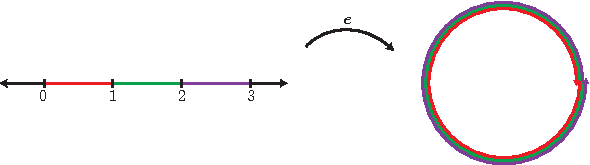
\includegraphics[width=240pt]{images/slinky-eps-converted-to.pdf}
\end{center}
%LEZ 20
	\subsection{Mappa esponenziale}
La \textbf{mappa esponenziale} $\funztot e \realset {S^1} t {e^{2\pi i t}}$ si può considerare come quoziente per l'azione di $\integerset$ su $\realset$, dunque è continua e \textit{aperta}. Con questa notazione si considera $S^1\subseteq\complexset$, per cui $S^1=\{z\in\complexset \mid |z|=1 \}$. Si considererà come punto base $(1,0) \in \realset^2$.

\subsubsection{Rivestimento}
Vogliamo ora utilizzare questa proprietà per definire il numero di giri che fa un cammino chiuso intorno alla circonferenza.
\begin{lemming} \label{teo uniformemente rivestito}
	Sia $U\subsetneqq S^1$ aperto. Allora $\displaystyle e^{-1}(U) = \amalg_{n\in\integerset} V_n$ con $V_n\subseteq\realset$ aperto e la restrizione $\funz {e_{|_{V_n}}} {V_n} U$ è un omeomorfismo $\forall n\in\integerset$.
\end{lemming}
\begin{define} \textsc{Uniformemente rivestito} \index{uniformemente rivestito} \\
	Un tale $U$ aperto di un qualsiasi spazio topologico $X$ si dice \textit{uniformemente rivestito}.
\end{define}
\begin{demonstration}
	Si consideri un punto non in $U$, ad esempio supponiamo che $1\notin U$. Si ha che $e^{-1}(1)=\{t \mid e^{2\pi i t}=\cos(2\pi t)+i\sin(2\pi t)=1\}=\integerset \implies \integerset \cap e^{-1}(U)=\emptyset$, ovvero $\integerset$ è disgiunto dalla controimmagine di $U$.\\
	Poniamo $V_0\coloneqq e^{-1}(U)\cap \intv= e^{-1}(U)\cap (0,\ 1)$ in quanto la controimmagine di $U$ non contiene interi. Si ha che $V_0$ è aperto in $\realset$ in quanto intersezione di aperti, la restrizione $e_{|_{V_0}}$ è iniettiva e $e(V_0)=U$ in quanto $e\left( (0,\ 1) \right)=S^1\setminus\left\{1\right\}$. Siccome $e$ è aperta allora la restrizione $\funz {e_{|_{V_0}}} {V_0} U$ è un omeomorfismo in quanto è biunivoca, continua e aperta.\\
	Poniamo $V_n\coloneqq V_0 +n=\{ x+n \mid x\in V_0\},\ \forall n\in\integerset$. Allora $\displaystyle e^{-1}(U)=\union_{n\in\integerset} V_n$ e $V_n\subseteq (n,\ n+1)$ quindi $V_n\cap V_m=\emptyset$ se $n\neq m$, che implica l'iniettività della funzione che segue. Siccome $e(V_n)=U$ allora $\funz  {e_{|_{V_n}}} {V_n} U$ è un omeomorfismo.
\end{demonstration}

\subsubsection{Sollevamento}

\begin{define} \textsc{Sollevamento} \index{sollevamento}\\
	\begin{minipage}[t]{0.73\textwidth}
		Sia $\alpha$ un cammino in $S^1$. Un \textbf{sollevamento} di $\alpha$ è una funzione \textit{continua} $\funz {\widetilde{\alpha}} I \realset$ tale che commuti il diagramma, ovvero  tale che $\alpha= e\circ \widetilde{\alpha}$. \\
		Più n generale, dato $X$ spazio topologico e $\funz f X {S^1}$ continua, un sollevamento di $f$ è $\funz {\widetilde{f}} X \realset$ continua tale che $f=e\circ \widetilde{f}$
	\end{minipage}
	\begin{minipage}[t]{0.13\textwidth}\vspace{-10pt}
		\begin{tikzcd}
			&  & \realset \arrow[dd, "e"] \\
			&  &                     \\
			I \arrow[rr, "\alpha"] \arrow[rruu, "\widetilde{\alpha}" , dashed] &  & S^1                
		\end{tikzcd}
	\end{minipage}
\end{define}
Se $\widetilde{\alpha}$ è un sollevamento di $\alpha$ allora
	\begin{equation*}
		\forall t\in I, \ (\widetilde{\alpha}(t))=\alpha(t)\implies e^{2\pi i \widetilde{\alpha}(t)}=\cos(2\pi \widetilde{\alpha}(t))+i\sin(2\pi\widetilde{\alpha}(t))=\alpha(t)
	\end{equation*}
Dunque $2\pi\widetilde{\alpha}(t)$ è una determinazione dell'angolo per $\alpha(t\in S^1)$, quindi muovendosi con continuità su $S^1$ tramite $\alpha$ ci si muove in maniera continua anche tramite $\alpha$, ovvero $2\pi\widetilde{\alpha}$ è una determinazione continua dell'angolo per $\alpha$.\\
Vediamo degli esempi.
\begin{examples}
	Fissato $n\in\integerset$, si considera il cammino $\funztot \gamma I {S^1} t {e^{2\pi i nt}}$. Per $n=1$ si percorre $1$ giro in senso \textit{antiorario}, con $n=2$ si percorrono $2$ giri in senso antiorario, con $n=-1$ si percorre $1$ un giro in senso \textit{orario}.\\ 
	Un sollevamento di $\gamma$ è dato da $\funz {\widetilde{y}} I {S^1}$ dove per condizione di essere sollevamento si ha che $\gamma(t)=e(\widetilde{\gamma}(t))$, quindi $\widetilde{\gamma}(t)=nt$, che ha una scrittura così facile perché $\gamma$ è già scritto in forma esponenziale.
\end{examples}
Andiamo ora a verificare l'esistenza di sollevamenti per cammini e vedere se e quando sono unici.
\begin{theorema} \textsc{Sollevamento di cammini} \label{teo sollevamento cammini}\\
	Ogni cammino $\funz \alpha I {S^1}$ ammette un sollevamento $\funz {\widetilde{\alpha}} I \realset$. Inoltre fissato il punto iniziale il sollevamento è unico, ovvero fissato $x_0\in\realset \colon e(x_0)=\alpha(0)$, vale a dire \\
	$x_0\in e^{-1}(\alpha(0))$ fibra di $\alpha(0)\in S^1$,  $\exists ! \funz {\widetilde{\alpha}} I \realset$ sollevamento di $\alpha$ \textit{a partire da $x_0$}, cioé $\widetilde{\alpha}(0)=x_0$.
\end{theorema}
\begin{demonstration}
	Per dimostrare l'\textit{esistenza} si sfruttano gli aperti uniformemente rivestiti, si divide $I$ in modo tale da avere sottointervalli la cui immagine tramite $\alpha$ sia contenuta in un aperto rivestito e sulla costruzione induttiva del sollevamento ‘‘a pezzi'' componendo con le inverse locali dell'esponenziale.\\
	Considerando tutti i punti della circonferenza, ovvero $\forall p\in S^1$, sia $U_p\subsetneqq S^1$ un intorno aperto connesso di $p$, allora $U_p$ è uniformemente rivestito, quindi $\{U_p\}_{p\in S^1}$ è un ricoprimento aperto di $S^1$.\\
	Sia $\funz \alpha I {S^1}$ un cammino, per il corollario \ref{corollario suddivisione} del teorema di Lebesgue si ha che $\exists\ 0=t_0\leq t_1\leq\dots\leq t_k=1$ suddivisione $\colon \forall i=1,\dots, k,\ \alpha([t_{i-1},\ t_i])\subseteq U_i$ aperto del ricoprimento. Costruiamo ora il sollevamento ‘‘a pezzi'' induttivamente su ciascun intervallino$[0,\ t_i]$: prima si costruisce il caso base per $[0,\ t_1]$ poi assumendo di aver già definito il sollevamento fino a $t_i$ lo si costruisce fino a $t_{i+1}$.\\ 
	Per $i=0$ poniamo $\widetilde{\alpha}(0)=x_0$. Si consideri l'intervallo $[0,\ t_1]$, si ha che $\alpha\left([0,\ t_1]\right)\subseteq U_1$ uniformemente rivestito, quindi per la proprietà di essere uniformemente rivestito (vedasi il lemma \ref{teo uniformemente rivestito}) $\displaystyle e^{-1}(U_1) = \amalg_{n\in\integerset}V_n$ aperto in $\realset$ tale che $\funz {e_{|_{V_n}}} {V_n} {U_1}$ è un omeomorfismo. Siccome $x_0\in e^{-1}(\alpha(0))$ e $\alpha(0)\in U_1$ allora $x_0\in e^{-1}(U_1)$, ma i $V_n$ sono disgiunti, quindi $\exists ! \overline{n} \colon x_0\in V_{\overline{n}}$. Siccome $\funz {e_{|_{V_{\overline{n}}}}} {V_{\overline{n}}} {U_1}$ è un omeomorfismo allora ha un'inversa locale $\funz {\phi\coloneqq \left(e_{|_{V_{\overline{n}}}}\right)^{-1}} {U_1} {V_{\overline{n}}}$.\\
	Poniamo ora come primo ‘‘pezzo'' del sollevamento $\widetilde{\alpha_1}\coloneqq \phi\circ \alpha_{|_{[0,\ t_1]}}$,  $\funz {\widetilde{\alpha_1}} {[0,\ t_1]} \realset$.
	Supponiamo di avere definito $\funz {\widetilde{\alpha_i}} {[0,\ t_i]} \realset$ continua, sollevamento di $\alpha_{|_{[0,\ t_i]}}$, ovvero il sollevamento di $\alpha$ da $0$ fino a $t_i$. Procedendo analogamente al primo intervallo, consideriamo $\alpha\left( [t_i,\ t_{i+1}] \right)\subseteq U_{i+1}$ uniformemente rivestito, allora $e^{-1}(U_{i+1})=\amalg_{m\in\integerset} W_m$ con $W_m$ aperti. Fra questi $W_m$ scegliamo quello che contiene il punto di partenza \\  $\widetilde{\alpha_i}(t_i)\in e^{-1}\left( \alpha(t_i) \right) \implies \widetilde{\alpha_i}(t_i)\in e^{-1}\left( U_{i+1} \right) \implies \exists ! \overline{m} \colon \widetilde{\alpha_i}(t_i)\in W_{\overline{m}}.$\\
	Sia $\funz {\psi\coloneqq \left( e_{|_{W_{\overline{m}}}} \right)^{-1}} {U_{i+1}} {W_{\overline{m}}}$ e poniamo $\funz {\widetilde{\alpha_{i+1}}} {[0,\ t_{i+1}]} \realset$ inversa locale che estende il sollevamento $\widetilde{\alpha_i}$ definita come segue $\widetilde{\alpha_{i+1}}(t)= \begin{cases}
			\widetilde{\alpha_i}(t) & t\in [0,\ t_i]\\
			\psi\circ \alpha(t) & t\in[t_i,\ t_{i+1}]
		\end{cases}$. Tale funzione è continua per il lemma di incollamento \ref{lemmaincollamento}, infatti è continua separatamente e per costruzione di incolla in $t_i$\\ 
	Procedendo in questo modo definiamo $\funz {\widetilde{\alpha}} \intv \realset$ sollevamento di $\alpha$ a partire da $x_0$. \\
	Dimostriamo ora l'\textit{unicità}. Sia $\funz {\widehat{\alpha}} \intv \realset$ un altro sollevamento di $\alpha$ a partire da $x_0$. Sia $Y \coloneqq \{t\in I \mid \widetilde{\alpha}(t)=\widehat{\alpha}(t)\}$ l'insieme dove $\widetilde{\alpha}$ e $\widehat{\alpha}$ coincidono. Si ha che $0\in Y \implies Y\neq\emptyset$, infatti $\widetilde{\alpha}(0)=\widehat{\alpha}(0)=x_0$  e $Y$ è chiuso, infatti per l'implicazione $1\Rightarrow 3)$ del teorema \ref{quoziente Hausdorff} si ha che date due mappe continue a valori in $T_2$, l'insieme su cui conincidono è chiuso. Mostriamo che $Y$ è anche aperto e connesso, così per laconnessione di $I$ si ha che $Y=I$, il che implica $\widetilde{\alpha}=\widehat{\alpha}$. Per dimostrare che $Y$ è aperto dimostriamo che è intorno di ogni suo punto, per farlo si sfruttano gli intorni uniformemente rivestiti.\\
	Sia $t_0\in Y$ e sia $\alpha(t_0)\in S^1$. Sia $U$ un intorno aperto di $\alpha(t_0)$ uniformemente rivestito, allora $e^{-1}(U)=\amalg_{n\in\integerset}V_n$, inoltre $\widetilde{\alpha}(t_0)=\widehat{\alpha}(t_0)\in e^{-1} \left( \alpha(t_0) \right)\subseteq e^{-1}(U)$ e per il lemma \ref{teo uniformemente rivestito} $\exists ! \overline{n} \colon \widetilde{\alpha} (t_0)=\widehat{\alpha}(t_0)\in V_{\overline{n}}$ aperto in $\realset$. \\
	Poniamo $A\coloneqq \widetilde{\alpha}^{-1}(V_{\overline{n}}) \cap \widehat{\alpha}^{-1}(V_{\overline{n\cap }})$. Si ha che $A$ è aperto in $I$ in quanto intersezione di controimmagine tramite funzioni continue di aperti e $t_0 \in A$. Mostriamo che le due funzioni coincidono su $A$, ovvero $\widetilde{\alpha}(t)=\widehat{\alpha}(t),\ \forall t\in A$. Se $t\in A$, per definizione di $A$ si ha che $\widetilde{\alpha}(t), \widehat{\alpha}(t)\in V_{\overline{n}}$ e per definizione di sollevamento $e\left( \widetilde{\alpha}(t) \right)= e\left( \widehat{\alpha}(t) \right)= \alpha(t)$ ma $e_{|_{V_{\overline{n}}}}$ è iniettiva perché è un omeomorfismo, quindi $\widetilde{\alpha}(t)=\widehat{\alpha}(t) \implies A\subseteq Y \implies t_0$ è interno a $Y \implies Y$ aperto.
\end{demonstration}

\subsubsection{Grado di un cammino}
\begin{define} \textsc{Grado di un cammino chiuso in $S^1$}\\
	Sia $\funz \alpha I {S^1}$ un cammino chiuso con punto base $1\in S^1$ e sia $\funz {\widetilde{\alpha}} I \realset$ l'unico sollevamento di $\alpha$ a partire da $x_0=0 \in e^{-1} (1)$. Si definisce \textbf{grado} di $\alpha$ come $\deg (\alpha)\coloneqq \widetilde{\alpha}(1)$
\end{define}

\begin{observe} \textsc{$\deg(\alpha)\in\integerset$}\\
	Quella appena data è una buona definizione grazie al teorema precedente che assicura che il grado esiste ed è unico. \\
	Inoltre $\deg(\alpha)\in\integerset$, infatti per definizione di sollevemento e siccome il cammino è chiuso $\widetilde{\alpha}(1)\in e^{-1}(\alpha(1))=e^{-1}(\alpha(0))=e^{-1}(1)=\integerset$\\
	Il grado conta il numero di giri con segno di $\alpha$ intorno a $S^1$, dove il segno è positivo se gira in senso antiorario, e negativo se gira in senso orario.
\end{observe}

Abbiamo così formalizzato il numero di giri con segno intorno a $S^1$, vediamo qualche esempio.
\begin{examples}
	\begin{itemize} 
		\item Sia $\alpha(t)=e^{2\pi i t}$, con $t\in\intv$, e sia $\widetilde{\alpha}(t)=t$ il sollevamento di $\alpha$ a partire da $x_0=0$. Siccome $\widetilde{\alpha}(1)=1\implies \deg\alpha=1$, ovvero $\alpha$ percorre solo un giro intono a $S^1$.
		\item Fissato $n\in\integerset$, sia $\displaystyle \funztot \gamma I {S^1} t {e^{2\pi i nt}}$, esso è un cammino chiuso con punto base $1$. Il sollevamento di $\gamma$ con punto base $x_0=0$ è dato da $\widetilde{\gamma}(t)=nt \implies \deg\gamma=\widetilde{\gamma}(1)=n.$
	\end{itemize}	
\end{examples}

\begin{observe} \textsc{$\deg\alpha = \widetilde{\alpha}(1)- \widetilde{\alpha}(0)$}\\
	Sia $\funz \alpha I {S^1}$ un cammino chiuso con punto base $1$. Sia $\widetilde{\alpha_0}$ il sollevamento di $\alpha$ con punto base $x_0=0$. Sia $n\in\integerset$ e sia $\funz {\widetilde{\alpha_n}} I \realset$ definita come $\widetilde{\alpha_n}=\widetilde{\alpha_0}+n$. 
	Siccome per ogni punto nella fibra del punto iniziale esiste ed è unico il sollevamento, e siccome la fibra in questo caso sono tutti gli interi si ha che per ogni intero si ha un sollevamento, che sarà il traslato di $\widetilde{\alpha_0}$. Verifichiamolo.\\
	Si ha che $\widetilde{\alpha_n}$ è continuo ed è un sollevamento di $\alpha$, infatti
		\begin{gather*}
			e\left( \widetilde{\alpha_n}(t) \right)= e^{2\pi i \widetilde{\alpha_n}(t)}= e^{2\pi i (\widetilde{\alpha_0}(t)+n)}=e^{2\pi i \widetilde{\alpha_0}(t)} e^{2\pi i n}=\alpha(t)
		\end{gather*}
	Il suo punto iniziale è $n$, infatti $\widetilde{\alpha_n}(0)=\widetilde{\alpha_0}(0)+n=n$.	Quindi $\widetilde{\alpha_n}$ è il sollevamento di $\alpha$ a partire da $x_0=n$.\\
	Inoltre osserviamo che 
		\begin{gather*}
			\widetilde{\alpha_n}(1)- \widetilde{\alpha_n}(0)=\widetilde{\alpha_0}(1)+n - (\underbrace{\widetilde{\alpha_0}(0)}_{=0}+n)= \widetilde{\alpha_0}(1)=\deg\alpha\\
			\implies \deg\alpha= \widetilde{\alpha}(1)-\widetilde{\alpha}(0)
		\end{gather*}
	con $\widetilde{\alpha}$ è un sollevamento qualsiasi.\\
	Si può quindi riformulare la definizione di grado di un cammino chiuso in $S^1$ con \textit{punto base qualsiasi} come la differenza fra il punto finale e quello iniziale di un sollevamento \textit{qualsiasi} del cammino.
\end{observe}

Vediamo ora come si comporta il grado rispetto al prodotto di cammini.
\begin{theorema}
	Siano $\alpha, \beta$ cammini chiusi in $S^1$ con punto base $1$. Allora $\deg(\alpha\ast\beta)=\deg\alpha +\deg\beta$
\end{theorema}
\begin{demonstration}
	Sia $\widetilde{\alpha}$ il sollevamento di $\alpha$ a partire da $x_0=0$, allora $a\coloneqq \widetilde{\alpha}(1)=\deg\alpha\in\integerset$. Sia $\widehat{\beta}$ il sollevamento di $\beta$ a partire da $a$, allora $\deg\beta=\widehat{\beta}(1)-\widehat{\beta}(0)=\widehat{\beta}-a$. Siccome $\funz {\widetilde{\alpha},\widehat{\beta}} I \realset$ e $\widetilde{\alpha}(1)=\widehat{\beta}(0)$ si può considerare il cammino prodotto $\funz {\widetilde{\alpha}\ast\widehat{\beta}} I \realset$. Dimostriamo che è un sollevamento di $\alpha\ast\beta$
		\begin{gather*}
			e\left( \widetilde{\alpha}\ast\widehat{\beta}(t) \right)= e^{2\pi i \widetilde{\alpha}\ast\widehat{\beta}(t)}=\begin{cases}
				e^{2\pi i \widetilde{\alpha}(t)}, & t\in \left[ 0,\ \frac{1}{2} \right]\\
				e^{2\pi i \widehat{\beta}(2t-1)}, & t\in \left[ \frac{1}{2},\ 1 \right]
			\end{cases}=\begin{cases}
				\alpha(2t), & t\in \left[ 0,\ \frac{1}{2} \right]\\
				\beta(2t-1), & t\in \left[ \frac{1}{2},\ 1 \right]
			\end{cases}= \alpha\ast\beta(t)\\
			(\widetilde{\alpha}\ast\widehat{\beta})(0)=\widetilde{\alpha}(0)=0 \implies \deg(\alpha\ast\beta)=(\widetilde{\alpha}\ast\widehat{\beta})(1)=\widehat{\beta}(1)=a+\deg\beta=\deg\alpha +\deg\beta 
		\end{gather*}
\end{demonstration}


Si ha che il grado è invariante per omotopia di cammini, tuttavia è un teorema che non dimostriamo, ma concettualmente consiste nel costruire un sollevamento fra le omotopie per mostrare che hanno lo stesso grado.
\begin{theorema} \textsc{di monodronia}\\
	Siano $\alpha,\beta$ cammini chiusi in $S^1$ con punto base $1$ e supponiamo che $\alpha$ e $\beta$ siano cammini omotopi. Allora $\deg\alpha=\deg\beta$, ovvero il grado è invariante per omotopia di cammini.
\end{theorema}

\subsubsection{Dimostrazione del gruppo fondamentale della circonferenza}
\begin{theorema}\textsc{Gruppo fondamentale di $S^1$}\\
	\begin{center}
		$\gruf{S^1}{1}\cong\integerset$
	\end{center}
\end{theorema}
\begin{demonstration}
	Sia $\displaystyle \funztot \Phi {\gruf{S^1}{1}} \integerset {[\alpha]} {\deg\alpha}$. Vogliamo dimostrare che è un isomorfismo di gruppi per ottenere la tesi.
		\begin{itemize}
			\item $\Phi$ è un'applicazione \textit{ben definita} per il teorema della monodronia.
			\item $\Phi$ è un \textit{morfismo di gruppi}, infatti dati $[\alpha],[\beta]\in\gruf{S^1}{1}$ si ha che
				\begin{gather*}
					\Phi([\alpha]\cdot [\beta])=\Phi([\alpha\ast\beta])=\det(\alpha\ast\beta)=\deg\alpha+\deg\beta=\Phi([\alpha])+\Phi([\beta])
				\end{gather*}
			\item $\Phi$ è \textit{suriettiva}, infatti $\forall n\in\integerset,\ \exists \gamma$ cammino chiuso in $S^1$ e di grado $n\implies \Phi([\gamma])=n$
			\item $\Phi$ è \textit{iniettiva}, mostriamo che $\ker\Phi$ è banale. Sia $[\alpha]\in\ker\Phi$, vogliamo dimostrare che $[\alpha]=[c_1]$, ovvero $\alpha\sim c_1$ cammino costante in $S^1$. Per ipotesi $\deg\alpha=\Phi([\alpha])=0$, quindi si considera il sollevamento di $\alpha$ con punto base $x_0=0$, quindi $\deg\alpha=\widetilde{\alpha}(1)=0$, cioè $\alpha$ è un cammino chiuso. Siccome $\realset$ è contraibile allora è semplicemente connesso, dunque $\gruf{\realset}{0}=\left\{1\right\}$ quindi $[\widetilde{\alpha}]\in\gruf{\realset}{0}=\left\{1\right\}\implies [\widetilde{\alpha}]=[c_0]\implies \exists \funz F {I\times I}  \realset$ omotopia di cammini fra $\widetilde{\alpha}$ e $c_0$, ovvero $F$ è continua e $F(t,0)=\widetilde{\alpha}(t),\ F(0,s)=F(1,s)=0,\ F(t,1)=0,\ \forall t,s\in I$. Sia $\funz {G\coloneqq e\circ F} {I\times I} {S^1}$, allora $G$ è continua e vale che 
				\begin{gather*}
					G(t,0)=e(F(t,0))=e(\widetilde{\alpha}(t))=\alpha(t)\\
					G(t,1)=e(F(t,1))=e(0)=1\\
					G(0,s)=G(1,s)=1,\ \forall t,s\in I
				\end{gather*}
			quindi $G$ è un'omotopia di cammini fra $\alpha$ e $c_1$ in $S^1\implies \Phi$ iniettiva $\implies \Phi$ isomorfismo di gruppi.
		\end{itemize}	
\end{demonstration}

%intermezzo LEZ 19
	\subsection{Conseguenze}
Osserviamo ora tramite un esempio sulla circonferenza che il corollario \ref{corollario van kampfen} non vale se $A$ e $B$ non sono aperti.
\begin{observe}
	Siano $X=S^1, A=(S^1\cap\{y>0\})\cup \{(1,0)\}$ e $B=S^1\cap\{y\leq 0\}$ che non sono aperti in $X$. Siccome $A\cong (0,\ 1]\subseteq \realset$ che è convesso in $\realset$ allora $A$ è contraibile e dunque semplicemente connesso. Analogamente per $B\cong\intv$. Dunque si ha che $X=A\cup B, A\cap B=\{(1,\ 0)\}\neq\emptyset$ e c.p.a., ma $X=S^1$ non è semplicemente connesso.
\end{observe}

\begin{corollary} \textsc{Manetti, 12.38} \label{circonferenza non retratto disco} \\
	Sia $D\subseteq\realset^2$ il disco unitario e $A=\partial{D}$ il bordo, ovvero $A=S^1$. Allora $A$ non è un retratto di $D$.
\end{corollary}
\begin{demonstration}
	Se $A$ fosse un retratto allora $\gruf{A}{\ }$ dovrebbe essere isomorfo ad un sottogruppo di $\gruf{D}{\ }$. Tuttavia $\gruf{A}{\ }=\gruf{S^1}{\ }=\integerset$ e $D\subseteq\realset^2$ convesso $\implies \gruf{D}{\ }=\left\{1\right\}$, il che non è possibile.
\end{demonstration}
\begin{observe}
	Allo stesso modo se $X$ è uno spazio topologico semplicemente connesso e $A\subseteq X$ con $A\cong S^1$, allora $A$ non può essere un retratto di $X$.
\end{observe}

\begin{corollary} \textsc{Teorema del punto fisso di Brouwer, Manetti 12.39} \label{punto fisso B} \index{punto fisso} \index{Brouwer} \\
	Sia $D\subseteq \realset^2$ il disco unitario e sia $\funz f D D$ continua. Allora $f$ ha un punto fisso, ovvero $\exists x_0\in D \colon f(x_0)=x_0$.
\end{corollary}
\begin{demonstration}
	Ragionando per assurdo supponiamo che $f$ non abbia punti fissi, ovvero $f(x_0)\neq x_0,\ \forall x_0\in D$. Utilizziamo $f$ per costruire una retrazione che non può esistere per motivi topologici: sia $\funz r D {\partial{D}}$ retrazione continua con $r_{\partial{D}}=Id_{\partial{D}}$ definita nel modo seguente. Sia $S$ la semiretta aperta uscente da $f(x)$ (essendo aperta il punto $f(x)$ è escluso) e passante per $x$, essa esiste perché $x\neq f(x)$ per ipotesi assurda, e si ponga $r(x)=S\cap\partial{D}$. Se $x\in\partial{D} \implies x=r(x) \implies r_{|_{\partial{D}}}= Id_{\partial{D}} \implies r$ retrazione, il che è assurdo per il corollario precedente.
\end{demonstration}
%fine intermezzo LEZ 19

\subsubsection{Invarianza della dimensione}
Grazie al calcolo del gruppo fondamentale della circonferenza si riescono anche a dimostrare dei casi particolari del teorema di invarianza della dimensione (che verrà affrontato nel corso di Topologia Algebrica), che recita quanto segue.
\begin{theorema}
	Siano $U\subseteq\realset^n$ e $V\subseteq \realset^m$ aperti. Se $U$ e $V$ sono omeomorfi allora $n=m$. Per contronominale, se $n\neq m$ allora $U$ e $V$ non sono omeomorfi.
\end{theorema}


\begin{observe}
	Sia $U\subseteq\realset^n$ aperto con $n\geq 2$. Allora $U$ non è omeomorfo ad un aperto di $\realset$. Per dimostrarlo basta considerare una palla $B$ in $\realset^n$ ed un intervallo $I$ in $\realset$ e togliere ad entrambe un punto: nel primo caso si ottiene ancora un connesso, mentre nel secondo uno sconnesso, dunque non possono essere omeomorfi.
\end{observe}
\begin{theorema}
	Sia $U\subseteq\realset^n$ aperto con $n\geq 3$. Allora $U$ non è omeomorfo ad un aperto di $\realset^2$.
\end{theorema}
\begin{demonstration}
	Ragionando per assurdo, ipotizziamo che $U$ sia omeomorfo ad un aperto di $\realset^2$. Sia $B\subseteq U$ una palla aperta di centro $p$, allora $B$ è omeomorfo ad un aperto $A$ di $\realset^2$. Sia $q\in A$ il punto corrispondente a $p$ tramite l'omeomorfismo, dunque $B\setminus\{p\}$ è omeomorfo a $A\setminus\{q\}$, ma $B\setminus\{p\}$ ha lo stesso tipo di omotopia di $S^{n-1}$, infatti sia $S$ una sfera centrata in $p$ tale per cui $S\subset B$, si ha che $S\cong S^{n-1}$ e $S\subset B\setminus\{p\}$ è un retratto di deformazione. Supponiamo per semplicità che $p=\mathbf{0}$: la retrazione è data da $\displaystyle \funztot r {B\setminus \{\mathbf{0}\}} S x {R\frac{x}{\| x \|}}$ con $R$ raggio di $S$, allora $A\setminus \{q\}$ ha lo stesso tipo di omotopia di $S^{n-1}, n\geq 3\implies n-1\geq 2\implies S^{n-1}$ è semplicemente connesso$\implies A\setminus\{q\}$ semplicemente connesso. Dimostriamo ora che questo è assurdo.\\
	$A$ aperto $\implies \exists C$ circonferenza centrata in $q$ tale che $C\subset A$. Si ha che $C$ è un retratto (in generale non di deformazione!) di $A\setminus\{q\}$, sempre con la stessa retrazione $\displaystyle \funztot f {A\setminus\{q\}} C {x=q+(x-q)} {q+r(C)\frac{x-q}{\| x-q \|}}$ con $r(C)$ raggio di $C$ e lo spostamento dovuto al fatto che $x$ non è il centro $q$. Se $x_0\in C\subset A\setminus\{q\}$ allora siccome è un retratto per il corollario \ref{grp fond iniettiva e suriettiva} si ha che $\integerset\cong \gruf{C}{x_0}\hookrightarrow \gruf{A\setminus\{q\}}{x_0} )=\left\{1\right\}$, da cui l'assurdo.
%LA FRECCIA NON è LUNGA QUANTO DOVREBBE
\end{demonstration}
\begin{attention}
	Non abbiamo potuto supporre che $A$ fosse una palla perché non sappiamo che ‘‘forma'' abbia dato l'omeomorfismo.
\end{attention}


	\subsection{Gruppo fondamentale prodotto}
	
\begin{theorema} \textsc{Manetti, 11.17}\\
	Siano $X$ e $Y$ spazi topologici, $x_0\in X$, $y_0\in Y$. Allora $\gruf{X\times Y}{(x_0,y_0)}\cong \gruf{X}{x_0}\oplus \gruf{Y}{y_0}$.
\end{theorema}
\begin{attention}
	Con $\oplus$ si intende la somma diretta di gruppi, da intendersi come prodotto cartesiano i cui morfismi sono componente per componente. Essa è diversa dalla somma diretta fra spazi vettoriali, in quest'ultimo caso infatti è interna!
\end{attention}
\begin{demonstration}
	Un cammino $\funz \alpha I {X\times Y}$ è determinato dalle sue componenti $\alpha=(\alpha_1,\ \alpha_2),\ \funz {\alpha_1} I X$ e $\funz {\alpha_2} I Y$, dunque c'è una corrispondenza biunivoca fra \\ $\inscam{X\times Y}{)x_0,\ y_0}{(x_0,\ y_0)}\leftrightarrow\inscam{X}{x_0}{x_0}\times \inscam{Y}{y_0}{y_0}$. Allo stesso modo le mappe $\funz F {I\times I} {X\times Y}$ è determinata dalle sue componenti $(F_1,\ F_2),\ \funz {F_1} {I\times I} X$ e $\funz {F_2} {I\times I} Y$, e inoltre si ha che $F$ è omotopia fra i cammini $\alpha$ e $\beta$ se e solo se $F_i$ è un'omotopia di cammini fra $\alpha_i$ e $\beta_i$. Dunque c'è una corrispondenza biunivoca tra i quozienti $\gruf{X\times Y}{(x_0,y_0)}\leftrightarrow \gruf{X}{x_0}\oplus \gruf{Y}{y_0}$ con $[\alpha]\leftrightarrow ([\alpha_1],\ [\alpha_2])$. Essa è anche un morfismo di gruppi, infatti $\alpha\ast\beta = (\alpha_1\ast\beta_1,\ \alpha_2\ast\beta_2)$, dunque i gruppi sono isomorfi.
\end{demonstration}

Analizziamo degli esempi di gruppi fondamentali.
\begin{example} \textsc{Toro}
	Si consideri lo spazio $S^1\times S^! =T$, detto toro. Siccome $S^1\subset\realset^2$ allora $T\subset \realset^4$, tuttavia esso è omeomorfo al sottospazio $X$ di $\realset^3$ visualizzato come una ‘‘ciambella''. Si può definire meglio come effetto della rotazione di una circonferenza attorno all'asse $z$ ad essa disgiunto.\\
	Per il teorema precedente si ha che $\gruf{T}{\ }=\gruf{T}{S^1\times S^1}=\integerset\oplus\integerset$. Siccome $\integerset$ è un gruppo ciclico infinito, posso considerare per il gruppo fondamentale gli analoghi di $\{-1\}$ e $\left\{1\right\}$, ovvero la classe del cappio di grado $1$ e quella di grado $-1$; si utilizzerà come generatore standard $\gamma(t)=e^{2\pi i t}$. Per il toro invece si considerano i generatori corrispondenti a $(1,\ 0)$ e $(0,\ 1)$ in $\integerset\oplus\integerset$, ovvero scelto il punto base $x_0=(1,\ 1)$, $\alpha(t)=(e^{2\pi i t},\ 1)$ e $\beta(t)=(1,\ e^{2\pi i t})$
\end{example}
%AAA COOL PICTURES CERCASI
%LEZ 21
\begin{example}\textsc{Gruppo fondamentale non abeliano}
	Sia $X$ l'unione ad un punto di due circonferenze in $\realset^2$, altresì detto bouquet di due circonferenze. Si ha che $\gruf{X}{x_0}$ è infinito ed i cammini per ogni circonferenza con punto base $x_0$ intersezione delle due circonferenze  $[\alpha]$ e $[\beta]$ non commutano, ovvero $[\alpha\ast\beta]\neq [\beta\ast\alpha]$. Inoltre $\gruf{X}{x_0}$ è generato da $[\alpha]$ e da $[\beta]$.
\end{example}	

	\subsection{Spazi proiettivi reali}
Consideriamo ora il caso degli spazi proiettivi reali. \\
Ricordiamo che la definizione \ref{def spazio proiettivo}, per cui $\mathbb{P}^n(\realset)=\nicefrac{\realset^{n+1}\setminus\{0\}}{\sim}$ dove $x\sim y \iff \exists\lambda\in\realset\setminus\{0\} \colon y=\lambda x$, ovvero $\sim$ indotta dall'azione di $\realset\setminus\{0\}$ su $\realset^{n+1}\setminus\{0\}$ per moltiplicazione. Ricordiamo anche la proposizione \ref{spazi proiettivi compatti connessi} per cui $\mathbb{P}^n(\realset)$ è compatto e connesso. Inoltre $\mathbb{P}^n(\realset)$ è $T_2$. Considerata la restrizione della proiezione $\funz {\pi_0\coloneqq \pi_{|_{S^n}}} {S^n} {\mathbb{P}^n(\realset)}$, essa è continua, suriettiva e chiusa (compatto in $T_2$), quindi $\pi_0$ è un'identificazione, ovvero $\mathbb{P}^n(\realset)$ è anche un quoziente di $S^n$ rispetto alla relazione che identifica i punti antipodali $p$ e $-p$. Si consideri la funzione associata $\funztot \phi {S^n} {S^n} p {-p}$ omeomorfismo di $S^n$. Tale relazione di equivalenza su $S^n$ è indotta dall'azione del gruppo $\{\pm 1\}$ per moltiplicazione, dunque $\funz {\pi_0} {S^n} {\mathbb{P}^n(\realset)}$ è sia chiusa sia aperta. In particolare, se $U\subset S^n$ è un aperto su cui $\pi_0$ è iniettiva, allora $\funz {\pi_{0_{|_{S^n}}}} U {\pi_0(U)}$ è un omeomorfismo perché continua, biunivoca e aperta. Da notare che se $\pi_0$ è iniettiva su $U$ allora $U\subsetneqq S^n$, dunque se $p_0\in S^n\setminus\{p_0\}\cong\realset^n \implies \pi_0(U)$ aperto in $\mathbb{P}^n(\realset)$ è omeomorfo ad un aperto di $\realset^n$.\\
Analizziamo dei casi di dimensione bassa:
	\begin{itemize}
		\item \underline{$n=1$} \textit{Retta proiettiva reale} $\mathbb{P}^1(\realset)$ 
		\item \underline{$n=2$} Il \textit{piano proiettivo reale}, la sua descrizione geometrica esplicita può essere complicata, per cui data la mappa $\funz {\pi_0	} {S^2} {\mathbb{P}^2(\realset)}$ e considerata la calotta superiore della sfera compreso l'equatore quale $C=\coloneqq S^2\cap\{z\geq 0\}$,si ha che $\pi_0(C)=\mathbb{P}^2(\realset)$, dunque $\funz {\pi_{0_{|_{C}}}} C {\mathbb{P}^2(\realset)}$ è ancora chiusa, dunque è ancora un'identificazione. Consideriamo ora un altro modello omeomorfo, detto \textit{modello piano di $\mathbb{P}^2(\realset)$}, quello del disco, che tuttavia non è omeomorfo a nesusn sottospazio di $\realset^3$, dunque non è rappresentabile. Sia $D\subset\realset^2$ il disco unitario; si ha che $D\cong\complexset$ tramite la proiezione ortogonale sul piano $x,y$, dunque $D\rightarrow \mathbb{P}^2(\realset)$ è un'identificazione che identifica i punti antipodali su $\partial{D}$. Inoltre il gruppo fondamentale $\pi_0(\mathbb{P}^2(\realset),\ p_0)=\nicefrac{\integerset}{2\integerset}$, infatti ho solo la classe di un cammino $\alpha$ fra due punti antipodali e quella del cammino costante $[c_0]$.
	\end{itemize}

\part{Classificazione delle superfici topologiche}
\labelPart{third}
% SVN info for this file
\svnidlong
{$HeadURL$}
{$LastChangedDate$}
{$LastChangedRevision$}
{$LastChangedBy$}

\chapter{Varietà topologiche}
\labelChapter{varietà}

\begin{introduction}
	‘‘BEEP BOOP INSERIRE CITAZIONE QUA BEEP BOOP.''
	\begin{flushright}
		\textsc{NON UN ROBOT,} UN UMANO IN CARNE ED OSSA BEEP BOOP.
	\end{flushright}
\end{introduction}

\section{Varietà topologiche}
%AAA INTRODUZIONE BELLA CERCASI
Si vuole formalizzare il concetto di avere la topologia euclidea localmente.
\begin{define}
	Uno spazio topologico $X$ si dice \textbf{localmente euclideo} di dimensione $n$ se ogni punto di $X$ ammette un intorno aperto omeomorfo ad una palla aperta di $\realset^n$.
\end{define}

\begin{define}
	Uno spazio topologico $X$ si dice \textbf{varietà topologica} di dimensione $n$ se $X$ è $T_2$, connesso, a base numerabile e localmente euclideo di dimensione $n$.
\end{define}

\begin{examples}
	\begin{itemize}
		\item $\realset^n$ è una varetà topologica di dimensione $n$
		\item $S^n$ è una varietà topologica compatta di dimensione $n$, infatti grazie alla proiezione stereografica si ha che $S^\setminus\{*\}\cong \realset$
		\item $\mathbb{P}^n(\realset)$ è una varietà topologica compatta di dimensione $n$
		\item ogni aperto connesso di una varietà topologica di dimensione $n$ è una varietà topologica di dimensione $n$
	\end{itemize}
\end{examples}
\begin{observe}
	La dimensione di una varietà topologica è ben definita per l'invarianza della dimensione.
\end{observe}
\begin{observe}
	Una varietà topologica è c.p.a.
%DIMOSTRAZIONE TUTORATO
	Se $X$ è una varietà topologica di dimensione $n$ e $Y$ è una varietà topologica di dimensione $m$ allora $X\times Y$ è una varità topologica di dimensione $n+m$.
%DIMOSTRAZIONE TUTORATO
\end{observe}
\begin{example}
	$T=S^1\times S^1$ è una varietà topologica di dimensione $2$.
\end{example}

\begin{theorema}
	Sia $X$ uno spazio topologico compatto, connesso, $T_2$ e localmente euclideo di dimensione $n$. Allora $X$ è a base numerabile, dunque $X$ è una varietà topologica di dimensione $n$.
\end{theorema}
 
	\subsection{Dimensione $1$}
Analizziamo il caso di varietà topologiche di dimensione $1$, per esempio $\realset$ e $S^1$.
\begin{theorema}
	Ogni varietà topologica di dimensione 1 è omeomorf a $\realset$ se non è compatta, oppure a $S^1$ se compatta.
\end{theorema} 
\begin{example} 
Riconsideriamo l'esempio della retta con 2 origini, vedasi la sezione \ref{retta 2 origini}, essa è un quoziente non $T_2$, dunque non è una varietà topologica.
\end{example}
	\subsection{Dimensione $2$}
\begin{define} 
	Una varietà topologica di dimensione 2 si dice \textbf{superficie topologica}.
\end{define}
\begin{examples}
	\begin{itemize}
		\item $\realset^2$ o $\realset^2\setminus \{n \text{punti}\}$ sono non compatti
		\item $S^2$ compatto
		\item $T=S^1\times S^1$ compatto
		\item $\mathbb{P}^2(\realset)$ compatto
	\end{itemize}
\end{examples}
Vogliamo dare una classificazione delle superfici topologiche \textit{compatte}. \footnote{Nota: seguiremo le note del professore Gianluca Occhetta}
%BIBLIOGRAFIA
\begin{examples} \textsc{modelli piani}\\
	\begin{itemize}
		\item Siccome $\mathbb{P}^2(\realset)$ è un quoziente del disco allora a meno di omeomorfismo lo si può anche vedere come un quoziente di $I\times I$ con una relazione di equivalenza sul bordo con parola $abab$
		% https://q.uiver.app/?q=WzAsNCxbMCwwLCJcXGJ1bGxldCJdLFsyLDAsIlxcYnVsbGV0Il0sWzIsMiwiXFxidWxsZXQiXSxbMCwyLCJcXGJ1bGxldCJdLFswLDEsImEiXSxbMSwyLCJiIl0sWzIsMywiYSJdLFszLDAsImIiXV0=
		\[\begin{tikzcd}
			{\bullet} && {\bullet} \\
			\\
			{\bullet} && {\bullet}
			\arrow["{a}", from=1-1, to=1-3]
			\arrow["{b}", from=1-3, to=3-3]
			\arrow["{a}", from=3-3, to=3-1]
			\arrow["{b}", from=3-1, to=1-1]
		\end{tikzcd}\]
		\item Anche il toro si può vedere come quoziente di $I\times I$ con parola $aba^{-1}b^{-1}$
		\begin{center}
			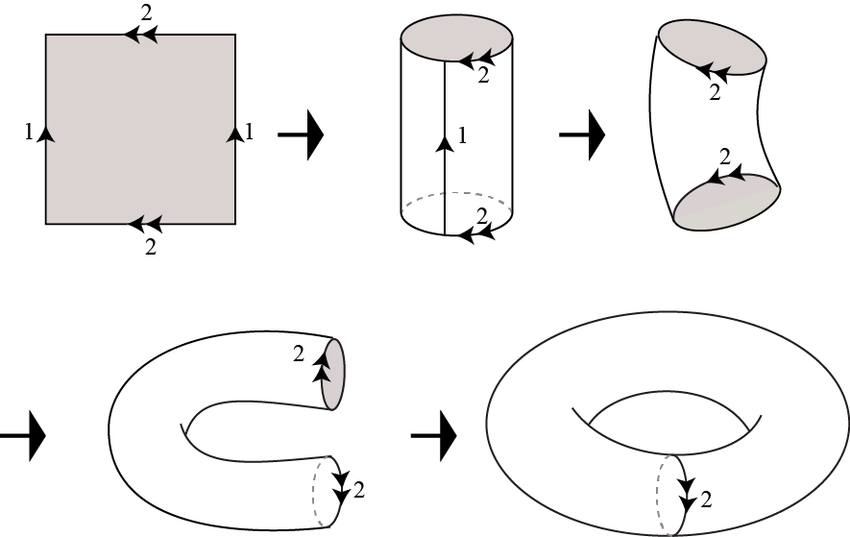
\includegraphics[trim=0cm 0 cm 0 cm, clip, scale=0.4]{images/The-construction-of-a-torus-from-the-unit-square.png}
		\end{center}
%IMMAGINE VENUTA MALE CON L'ENVIRONMENT
		\item Vediamo $S^2$ come quoziente di $I\times I$ con parola $bb^{-1}a^{-1}a$
		% https://q.uiver.app/?q=WzAsNCxbMCwwLCJcXGJ1bGxldCJdLFsyLDAsIlxcYnVsbGV0Il0sWzIsMiwiXFxidWxsZXQiXSxbMCwyLCJcXGJ1bGxldCJdLFswLDEsImIiXSxbMywwLCJhIl0sWzIsMSwiYiIsMl0sWzMsMiwiYSIsMl1d
		\[\begin{tikzcd}
			{\bullet} && {\bullet} \\
			\\
			{\bullet} && {\bullet}
			\arrow["{b}", from=1-1, to=1-3]
			\arrow["{a}", from=3-1, to=1-1]
			\arrow["{b}"', from=3-3, to=1-3]
			\arrow["{a}"', from=3-1, to=3-3]
		\end{tikzcd}\]
	\end{itemize}
\end{examples}

\begin{observe}
	Sia $P\subset\realset^2$ un poligono pieno con un numero pari di lati. Sia $\sim$ una relazione di equivalenza che identifica i lati a 2 a 2. Allora $S\coloneqq\nicefrac{P}{\sim}$ è una superficie topologica compatta, infatti
		\begin{enumerate}
			\item  $P$ è connesso e compatto $\implies S$ connesso e compatto
			\item $S$ è localmente euclideo di dimensione $2$. Sia $p\in S$, se $p$ viene da un punto interno al poligono allora si sceglie un intorno aperto $U$ centrato in tale punto tale che $U\cap\partial{P}=\emptyset$, data la proiezione $\funz \pi P S$, $\pi(U)\cong U$ ed è un intorno aperto di $p$. Se $p$ viene da un punto interno ad un lato grazie all'dentificazione dei lati a due a due si ha che passando al quoziente cìè un intorno aperto di $p$ omeomorfo ad un disco aperto. Se $p$ viene da un vertice, siccome i vertici vengono identificati con i vertici, analogamente al caso dei lati si ottiene un intorno aperto di $p$ in $S$ omeomorfo ad un disco aperto di $\realset^2$.
			\item $S$ è $T_2$.
		\end{enumerate}
	Osserviamo che nella relazione di equivalenza due lati vengono identificati nel modo seguente: $l_i\cong\intv$, dunque scelgo un omeomorfismo $l_1\stackrel{\stackrel{\phi}{\sim}}{\longrightarrow} l_2$, $p_1\in l_1 \sim \phi(p)\in l_2$ e $\phi$ manda vertici in vertici.
	Il poligono $P$ con la relazione di equivalenza sui lati è detto un \textbf{modello piano} della superficie $S$ e può essere schematizzato con una sequenza di lettere detta \textbf{parola}. Ad essempio per la parola $aba^{-1}cbc^{-1}$ si ottiene il modello piano sguente
	% https://q.uiver.app/?q=WzAsNixbMSwwLCJcXGJ1bGxldCJdLFsyLDAsIlxcYnVsbGV0Il0sWzMsMSwiXFxidWxsZXQiXSxbMCwxLCJcXGJ1bGxldCJdLFsxLDIsIlxcYnVsbGV0Il0sWzIsMiwiXFxidWxsZXQiXSxbMCwxLCJhIl0sWzEsMiwiYiJdLFswLDMsImMiLDJdLFs0LDMsImIiXSxbNSwyLCJhIiwyXSxbNSw0LCJjIl1d
	\[\begin{tikzcd}
		& {\bullet} & {\bullet} \\
		{\bullet} &&& {\bullet} \\
		& {\bullet} & {\bullet}
		\arrow["{a}", from=1-2, to=1-3]
		\arrow["{b}", from=1-3, to=2-4]
		\arrow["{c}"', from=1-2, to=2-1]
		\arrow["{b}", from=3-2, to=2-1]
		\arrow["{a}"', from=3-3, to=2-4]
		\arrow["{c}", from=3-3, to=3-2]
	\end{tikzcd}\]
 Inoltre il modello piano di una superficie compatta non è unico.
\end{observe}



\begin{examples}
	\begin{itemize}
		\item $S^2$
		% https://q.uiver.app/?q=WzAsMixbMCwwLCJcXGJ1bGxldCJdLFswLDIsIlxcYnVsbGV0Il0sWzAsMSwiYSIsMix7ImN1cnZlIjozfV0sWzAsMSwiYSIsMCx7ImN1cnZlIjotM31dXQ==
		\[\begin{tikzcd}
			{\bullet} \\
			\\
			{\bullet}
			\arrow["{a}"', from=1-1, to=3-1, curve={height=18pt}]
			\arrow["{a}", from=1-1, to=3-1, curve={height=-18pt}]
		\end{tikzcd}\]
		\item $\mathbb{P}^2(\realset)$
		% https://q.uiver.app/?q=WzAsMixbMCwwLCJcXGJ1bGxldCJdLFswLDIsIlxcYnVsbGV0Il0sWzAsMSwiYSIsMix7ImN1cnZlIjozfV0sWzEsMCwiYSIsMix7ImN1cnZlIjozfV1d
		\[\begin{tikzcd}
			{\bullet} \\
			\\
			{\bullet}
			\arrow["{a}"', from=1-1, to=3-1, curve={height=18pt}]
			\arrow["{a}"', from=3-1, to=1-1, curve={height=18pt}]
		\end{tikzcd}\]
		\item bottiglia di Klein $K$, essa è la superficie compatta data dal modello piano. Confrontiamolo con il toro. Incolliamo entrambi i modelli: prima si ottiene $S^1\times I$ con la relazione di equivalenza sul bordo.
		% https://q.uiver.app/?q=WzAsMTYsWzAsNCwiXFxidWxsZXQiXSxbMCw2LCJcXGJ1bGxldCJdLFsyLDQsIlxcYnVsbGV0Il0sWzIsNiwiXFxidWxsZXQiXSxbNSw0LCJcXGJ1bGxldCJdLFs3LDQsIlxcYnVsbGV0Il0sWzUsNiwiXFxidWxsZXQiXSxbNyw2LCJcXGJ1bGxldCJdLFswLDIsIlxcYnVsbGV0Il0sWzAsMCwiXFxidWxsZXQiXSxbMiwwLCJcXGJ1bGxldCJdLFsyLDIsIlxcYnVsbGV0Il0sWzUsMiwiXFxidWxsZXQiXSxbNSwwLCJcXGJ1bGxldCJdLFs3LDAsIlxcYnVsbGV0Il0sWzcsMiwiXFxidWxsZXQiXSxbMCwxLCIiLDIseyJzdHlsZSI6eyJoZWFkIjp7Im5hbWUiOiJub25lIn19fV0sWzIsMywiIiwyLHsic3R5bGUiOnsiaGVhZCI6eyJuYW1lIjoibm9uZSJ9fX1dLFswLDIsImIiLDIseyJjdXJ2ZSI6Mn1dLFswLDIsIiIsMSx7ImN1cnZlIjotMiwic3R5bGUiOnsiaGVhZCI6eyJuYW1lIjoibm9uZSJ9fX1dLFszLDEsImIiLDAseyJjdXJ2ZSI6LTJ9XSxbMSwzLCIiLDAseyJjdXJ2ZSI6LTIsInN0eWxlIjp7ImJvZHkiOnsibmFtZSI6ImRvdHRlZCJ9LCJoZWFkIjp7Im5hbWUiOiJub25lIn19fV0sWzQsNSwiYiIsMix7ImN1cnZlIjoyfV0sWzQsNSwiIiwwLHsiY3VydmUiOi0yLCJzdHlsZSI6eyJoZWFkIjp7Im5hbWUiOiJub25lIn19fV0sWzYsNywiYiIsMix7ImN1cnZlIjoyfV0sWzYsNywiIiwwLHsiY3VydmUiOi0yLCJzdHlsZSI6eyJib2R5Ijp7Im5hbWUiOiJkb3R0ZWQifSwiaGVhZCI6eyJuYW1lIjoibm9uZSJ9fX1dLFs0LDYsIiIsMSx7InN0eWxlIjp7ImhlYWQiOnsibmFtZSI6Im5vbmUifX19XSxbNSw3LCIiLDEseyJzdHlsZSI6eyJoZWFkIjp7Im5hbWUiOiJub25lIn19fV0sWzgsOSwiYSJdLFs5LDEwLCJiIl0sWzExLDEwLCJhIiwyXSxbMTEsOCwiYiJdLFsxMiwxMywiYSJdLFsxMywxNCwiYiJdLFsxMiwxNSwiYiIsMl0sWzE1LDE0LCJhIiwyXV0=
		\[\begin{tikzcd}
			{\bullet} && {\bullet} &&& {\bullet} && {\bullet} \\
			\\
			{\bullet} && {\bullet} &&& {\bullet} && {\bullet} \\
			\\
			{\bullet} && {\bullet} &&& {\bullet} && {\bullet} \\
			\\
			{\bullet} && {\bullet} &&& {\bullet} && {\bullet}
			\arrow[from=5-1, to=7-1, no head]
			\arrow[from=5-3, to=7-3, no head]
			\arrow["{b}"', from=5-1, to=5-3, curve={height=12pt}]
			\arrow[from=5-1, to=5-3, curve={height=-12pt}, no head]
			\arrow["{b}", from=7-3, to=7-1, curve={height=-12pt}]
			\arrow[from=7-1, to=7-3, curve={height=-12pt}, dotted, no head]
			\arrow["{b}"', from=5-6, to=5-8, curve={height=12pt}]
			\arrow[from=5-6, to=5-8, curve={height=-12pt}, no head]
			\arrow["{b}"', from=7-6, to=7-8, curve={height=12pt}]
			\arrow[from=7-6, to=7-8, curve={height=-12pt}, dotted, no head]
			\arrow[from=5-6, to=7-6, no head]
			\arrow[from=5-8, to=7-8, no head]
			\arrow["{a}", from=3-1, to=1-1]
			\arrow["{b}", from=1-1, to=1-3]
			\arrow["{a}"', from=3-3, to=1-3]
			\arrow["{b}", from=3-3, to=3-1]
			\arrow["{a}", from=3-6, to=1-6]
			\arrow["{b}", from=1-6, to=1-8]
			\arrow["{b}"', from=3-6, to=3-8]
			\arrow["{a}"', from=3-8, to=1-8]
		\end{tikzcd}\]
	\end{itemize}
\end{examples}

	\subsection{Somma connessa}
Siano $S_1$ e $S_2$ superfici compatte e siano $x\in S_1$ e $y\in S_2$. Siano $D_x\subset S_1$ e $D_y\subset S_2$ intorni di $x$ e $y$ rispettivamente, omeomorfi ad un disco chiuso $D\subset\realset^2$, dunque $D_x\stackrel{\stackrel{h}{\sim}}{\longrightarrow} D_y$. Togliamo dalle due superfici gli intorni dei dischetti, sia $Y\coloneqq (S_1\setminus \interior{D_x})\amalg (S_2\setminus \interior{D_y})$, incolliamo i due pezzi di $Y$ lungo i bordi dei dischi, cioé mettiamo su $Y$ la relazione di equivalenza $x_1\sim y_1 \iff x_1=y_1$ oppure $x_1\in\partial{D},\ y_1\in\partial{D}$ e $y_1=h(x_1)$ o viceversa.\newline
Vediamo ora qualche fatto che non dimostriamo:
	\begin{itemize}
		\item il quoziente è ancora una superficie topologica, che denotiamo con $S_1\# S_2$ \textbf{somma connessa} di $S_1$ e $S_2$
		\item la somma connessa $S_1\# S_2$ a meno di omeomorfismo non dipende dalle scelte fatte come i punti $x$ e $y$, gli intorni $D_x$ e $D_y$, l'omeomorfismo $h$, ma soltanto da $S_1$ e da $S_2$!
	\end{itemize}




%% SVN info for this file
\svnidlong
{$HeadURL$}
{$LastChangedDate$}
{$LastChangedRevision$}
{$LastChangedBy$}

\chapter{Approfondimenti di Algebra Lineare}
\labelChapter{jordan}

\begin{introduction}
	‘‘BEEP BOOP INSERIRE CITAZIONE QUA BEEP BOOP.''
	\begin{flushright}
		\textsc{NON UN ROBOT,} UN UMANO IN CARNE ED OSSA BEEP BOOP.
	\end{flushright}
\end{introduction}
% inserire citazione
\noindent Questo capitolo si può considerare un approfondimento di concetti ben noti dall'Algebra Lineare, cercando di rispondere alle seguenti questioni:
\begin{itemize}
	\item \textbf{\textsc{Diagonalizzazione simultanea}}: quando possiamo diagonalizzare due matrici con una \textit{stessa base} di autovettori?
	\item \textbf{\textsc{Polinomi e matrici}}: possiamo valutare un \textit{polinomio} con dei valori matriciali? Che relazione c'è fra polinomi matriciali e il \textit{polinomio caratteristico} della matrice?
	\item \textbf{\textsc{Forma canonica di Jordan}}: possiamo generalizzare la \textit{decomposizione spettrale} anche a matrici che non sono diagonalizzabili, rendendole così ‘‘più semplici''?
	\item \textbf{\textsc{Funzione esponenziale matriciale}}: come abbiamo fatto con i polinomi, possiamo ‘‘matricizzare'' la funzione esponenziale?
\end{itemize}
\section{Diagonalizzazione simultanea}
\begin{remember}
	Sia $V$ spazio vettoriale, su campo $\kamp$, di dimensione finita. Consideriamo gli \textbf{endomorfismi} di $V$ o, equivalentemente, le matrici $n\times n$ a elementi in $\kamp$ (con $\dim V=n$).
	\begin{itemize}
		\item $A$ determina un endomorfismo di $\kamp^n$ dato da $v\mapsto A\mathbf{v}$.
		\item Matrici associate allo stesso endomorfismo rispetto a basi diverse sono \textbf{simili}\index{matrice!simile}, cioè:
		\begin{equation}
			\exists P\in\gl\left(n\, \kamp\right)\ \colon B=P^{-1}AP
		\end{equation}
		\item Le seguenti affermazioni sono equivalenti:
		\begin{itemize}
			\item $A$ è \textbf{diagonalizzabile}\index{diagonalizzazione}.
			\item $A$ è simile ad una matrice diagonale $A=PDP^{-1}$ con $P$ matrice con \textbf{autovettori} sulle colonne.
			\item $\kamp^n$ ammette una base di \textbf{autovettori}\index{autovettore} di $A$.
			\item $\kamp^n=V_{\lambda_1}\oplus\ldots\oplus V_{\lambda_r}$ con $V_{\lambda_i}$ \textbf{autospazio}\index{autospazio} relativo ad $A$
		\end{itemize}
	\end{itemize}
\vspace{-3mm}
\end{remember}
\begin{define}[Diagonalizzazione simultanea.]~{}\\
	Siano $A,\ B\in\kamp^{n, m}$ due matrici \textit{diagonalizzabili}. Diciamo che $A$ e $B$ sono \textbf{simultaneamente diagonalizzabili}\index{diagonalizzazione!simultanea} se esiste una base di $\kamp^n$ composta di autovettori sia di $A$ che di $B$.\\
	Equivalentemente, $A$ e $B$ sono \textbf{simultaneamente diagonalizzabili} se esiste una matrice invertibile $P$ tale che $P^{-1}AP$ e $P^{-1}BP$ sono \textit{entrambe diagonali}.
\end{define}
\begin{example}
	Non tutte le matrici diagonalizzabili lo sono simultaneamente. Prendiamo $\realset^2$; si consideri:
	\begin{itemize}
		\item $A$ diagonalizzabile con $2$ autovalori diversi, i cui autospazi sono le rette $y=x$ e $y=-x$.
		\item $B$ diagonalizzabile con $2$ autovalori diversi, i cui autospazi sono le rette $y=0$ e $y=2x$.
	\end{itemize}
Non esiste alcun autovettore comune, dunque $A$ e $B$ \textit{non} sono simultaneamente diagonalizzabili.
\end{example}
Dalla sola definizione non è semplice capire quali matrici sono a tutti gli effetti simultaneamente diagonalizzabili. Tuttavia, il seguente teorema ci permetterà di trovare una condizione necessaria e sufficiente per la diagonalizzazione simultanea.
\begin{theorema}[Diagonalizzazione simultanea se e solo se le matrici diagonalizzabili commutano.]~{}\\ \label{teoremasimdiag}
	Siano $A,\ B\in\kamp^{n, n}$. Allora $A$ e $B$ sono simultaneamente diagonalizzabili se e solo se $A$ e $ B$ sono diagonalizzabili e $A,\ B$ commutano, cioè $AB=BA$.
\end{theorema}
Per dimostrare il teorema, abbiamo tuttavia bisogno del seguente lemma:
\begin{lemming}[Matrici che commutano e autospazi.]~{}\\
	Siano $A,\ B\in\kamp^{n, n}$ tale che $AB=BA$ e sia $W$ un autospazio di $B$. Allora, presa l'azione di $\gl\left(n,\ \kamp\right)$ su $\kamp^{n, n}$, si ha che $A\ldotp W\subseteq W$.
\end{lemming}
\begin{demonstration}
	Sia $\lambda$ l'autovalore di $B$ relativo all'autospazio $W$. Per definizione di autospazio:
	\begin{equation*}
		W=\left\{\mathbf{v}\in V\mid B\ldotp \mathbf{v}=\lambda \mathbf{v}\right\}
	\end{equation*}
Sia $\mathbf{w}\in W$. Vogliamo mostrare che $A\ldotp \mathbf{w}\in W$.
\begin{equation*}
	B\ldotp\left(A\ldotp\mathbf{w}\right)=\left(BA\ldotp\mathbf{w}\right)=\left(AB\ldotp\mathbf{w}\right)=A\ldotp\left(B\ldotp\mathbf{w}\right)=A\ldotp\left(\lambda\mathbf{w}\right)=\lambda\left(A\ldotp\mathbf{w}\right)
\end{equation*}
$A\ldotp \mathbf{w}$ è autovettore rispetto a $\lambda$, pertanto $A\ldotp \mathbf{w}\in W,\ \forall \mathbf{w}$ e dunque segue la tesi.
\end{demonstration}
\begin{demonstration} \textsc{Dimostrazione del teorema} \ref{teoremasimdiag}.\\
	$\impliesdx$ Per ipotesi, $\exists P\in \gl\left(n,\ \kamp\right)$ tale che $D_1=P^{-1}AP$ e $D_2=P^{-1}BP$ sono diagonali; in particolare, in quanto matrici diagonali, esse commutano: $D_1D_2=D_2D_1$. Allora $A=PD_1P^{-1}$ e $B=PD_2P^{-1}$.
	\begin{equation*}
		AB=\left(PD_1P^{-1}\right)\left(PD_2P^{-1}\right)=PD_1D_2P^{-1}=PD_2D_1P^{-1}=\left(PD_2P^{-1}\right)\left(PD_1P^{-1}\right)=BA
	\end{equation*}
$\impliessx$ Procediamo con una \textit{dimostrazione costruttiva}. Sappiamo che:
\begin{itemize}
	\item $A$ diagonalizzabile $\implies \exists \mathbf{v}_1,\ \ldots,\ \mathbf{v}_n$ base di $V$ composta da \textit{autovettori} di $A$.
	\item $B$ diagonalizzabile $\implies V=W_1\oplus\ldots\oplus W_r$ con $W_j$ \textit{autospazi} di $B$
\end{itemize}
Consideriamo $\mathbf{v}_1\in V$. Esso si scrive in modo unico:
\begin{equation*}
	\textcolor{red}{\circled{{\ast}}}\quad \mathbf{v}_1=\mathbf{w}_{1,1}+\ldots+\mathbf{w}_{1,r}\text{ con }\mathbf{w}_{1,j}\in W_j,\ \forall j=1,\ \ldots,\ r
\end{equation*}
$\mathbf{v}_1$ è autovettore di $A$ relativo all'autovalore di $\lambda_1$, dunque $A\mathbf{v}_1=\lambda_1\mathbf{v}$. \textit{Moltiplichiamo} $\mathbf{v}_1$ per $A$:
\begin{equation*}
	\begin{array}{ccc}
		A\ldotp\mathbf{v}_1&=&A\ldotp\mathbf{w}_{1,1}+\ldots+A\ldotp\mathbf{w}_{1,r}\\
		\shortparallel&\\
		\lambda_1\mathbf{v}_1&=&\lambda_1\mathbf{w}_{1,1}+\ldots+\lambda_1\mathbf{w}_{1,r}
	\end{array}
\end{equation*}
Dal lemma appena dimostrato, da $A\ldotp W_j\subseteq W_j,\ \forall j$ segue che $A\ldotp \mathbf{w}_j\in W_j$. Per la chiusura di $W_j$ rispetto al prodotto per uno scalare, abbiamo anche $\lambda \mathbf{w}_j\in W_j,\ \forall j$. Siccome in una somma diretta la decomposizione è unica, deduciamo che:
\begin{equation*}
	A\ldotp \mathbf{w}_{1,1}=\lambda_1 \mathbf{w}_{1,1},\ \ldots,\ A\ldotp \mathbf{w}_{1,r}=\lambda_1 \mathbf{w}_{1,r}
\end{equation*}
In altre parole, $\forall j,\ \mathbf{w}_{1,j}$ è $\mathbf{0}$ oppure un autovettore di $A$ e, per ipotesi, anche di $B$. Procediamo allo stesso modo tutti i vettori della base $\mathbf{v}_1, \ldots,\ \mathbf{v}_n$: si ha che $\mathbf{v}_i=\mathbf{w}_{i,1}+\ldots+\mathbf{w}_{i,r}$ e $\forall i, j,\ $ $\mathbf{w}_{i,j}$ è $\mathbf{0}$ oppure un autovettore comune di $A$ e $B$.\\
Otteniamo un insieme $\left\{\mathbf{w}_{i, j}\right\}$ di autovettori comuni di $A$ e $B$. Per costruzione, lo \textit{span lineare} dei $\left\{\mathbf{w}_{i, j}\right\}$ contiene $\left\{\mathbf{v}_1,\ \ldots,\ \mathbf{v}_n\right\}$ e pertanto è necessariamente pari a $V$!\\
In altre parole, $\left\{\mathbf{w}_{i,\ j}\right\}$ è un sistema di generatori di $V$ e possiamo estrarre da esso una base di $V$ costituita di autovettori comuni ad $A$ e a $B$.
\end{demonstration}
\section{Polinomi e matrici}
\begin{remember}
	Dato un campo $\kamp$, indichiamo con $\kamp\left[t\right]$ l'anello dei polinomi a coefficienti in $\kamp$ nella variabile $t$; un suo elemento $f\left(t\right)\in\kamp\left[t\right]$ è della forma:
	\begin{equation}
		f\left(t\right)=b_nt^n+b_{n-1}t^{n-1}+\ldots+b_1t+b_0\text{ con }b_i\in\kamp
	\end{equation}
\vspace{-6mm}
\end{remember}
Finora abbiamo sempre \textit{valutato} i polinomi in valori del campo $\kamp$. Possiamo invece valutarli in una \textit{matrice} in $\kamp^{n, n}$? Dopotutto, la \textit{somma di matrici} e la \textit{moltiplicazione per uno scalare} sono operazioni \textit{interne} a $\kamp^{n, n}$ e pertanto potremmo pensare che sia lecito.\\ Tuttavia, presi i polinomi $p$ così come sono, non sarebbe \textit{ben definita} $p\left(A\right)$ a causa del \textbf{termine noto}; infatti, non possiamo sommare uno \textit{scalare ad una matrice}! Per ovviare a questo problema, quando valutiamo un polinomio in una matrice $A$ ‘‘\textit{correggiamo}'' il termine noto con la \textbf{matrice identità} $I$:
\begin{equation}
	f\left(A\right)\coloneqq b_nA^n+b_{n-1}A^{n-1}+\ldots+b_1A+b_0I\text{ con }b_i\in\kamp
\end{equation}
In questo modo, $f\left(A\right)\in\kamp^{n, n}$.
\begin{example}
Preso $f\left(t\right)=t^2-3$, il polinomio valutato nella matrice $A$ è $f\left(A\right)=A^2-3I$.
\end{example}
\begin{observe}
	Dati $f,\ g\in\kamp\left[t\right]$ e $A\in\kamp^{n,n}$, si ha:
	\begin{itemize}
		\item $\left(f+g\right)\left(A\right)=f\left(A\right)+g\left(A\right)$.
		\item $\left(fg\right)\left(A\right)=f\left(A\right)g\left(A\right)$
	\end{itemize}
\vspace{-3mm}
\end{observe}
\begin{demonstration}
	Prendiamo i polinomi $f\left(t\right)=b_nt^n+b_{n-1}t^{n-1}+\ldots+b_1t+b_0$ e $g\left(t\right)=c_nt^n+c_{n-1}t^{n-1}+\ldots+c_1t+c_0$ e valutiamoli entrambi in $A$: $f\left(A\right)=b_nA^n+b_{n-1}A^{n-1}+\ldots+b_1A+b_0I$ e $g\left(A\right)=c_nA^n+c_{n-1}A^{n-1}+\ldots+c_1A+c_0I$.
	\begin{enumerate}[label=\Roman*]
		\item La somma è ovvia.
		\item Il prodotto è garantito dalla commutatività delle potenze di matrici.
	\end{enumerate}
\vspace{-3mm}
\end{demonstration}
\subsection{Ideale di una matrice}
\begin{define}[Ideale di una matrice.]~{}\\
	Data $A\in\kamp^{n,n}$, definiamo l'\textbf{ideale della matrice}\index{ideale!di una matrice}:
	\begin{equation}
		I_A\coloneqq\left\{f\in\kamp\left[t\right]\mid f\left(A\right)=O\right\}
	\end{equation}
\vspace{-6mm}
\end{define}
\begin{observe}~{}
	\begin{itemize}
		\item $O\in I_A$.
		\item $I_A\neq\left\{O\right\}$; infatti, se consideriamo le seguenti $n^2+1$ matrici in $\kamp^{n,n}$:
		\begin{equation*}
			I,\ A,\ A^2,\ A^3,\ \ldots,\ A^{n^2}
		\end{equation*}
	Per il lemma di Steinitz queste matrici sono necessariamente \textit{linearmente dipendenti}, dato che superano in numero $\dim \kamp^{n,n}=n^2$, cioè esistono i coefficienti $a_0,\ \ldots,\ a_{n^2}\in\kamp$ \textit{non} tutti nulli tali che:
	\begin{equation*}
		a_0I+a_1A+a_2A^2+\ldots+a_{n^2}A^{n^2}=O
	\end{equation*}
	Allora $p\left(t\right)=a_{n^2}t^{n^2}+\ldots+a_2t^2+a_1t+a_0$ è un polinomio \textit{non} nullo in $I_A$.
	\item $I_A$ soddisfa giustamente la definizione di ideale di $\kamp\left[t\right]$:
	\begin{itemize}
		\item \textsc{$I_A$ è un sottogruppo di $\left(\kamp^{n, n},\ +\right)$}.
		\begin{equation*}
			\left(f+g\right)\left(A\right)=f\left(A\right)+g\left(A\right)=0\implies f+g\in I_A
		\end{equation*}
		\item \textsc{Assorbimento}: se $h\in\kamp\left[t\right]$ si ha :
		\begin{equation*}
			\left(fh\right)\left(A\right)=\underbrace{f\left(A\right)}_{=O}h\left(A\right)=O\implies fh\in I_A
		\end{equation*}
	\end{itemize}
	\end{itemize}
\vspace{-3mm}
\end{observe}
\subsection{Polinomio minimo}
\begin{proposition}[Anello ${\kamp\left[t\right]}$ è ad ideali principali.]~{}\\
	L'anello $\kamp\left[t\right]$ è ad \textit{ideali principali}: se $I\subseteq \kamp\left[t\right]$ è un ideale, $\exists p$ tale che $I=\left(p\right)$. Il generatore $p$ è \textit{unico} a meno di moltiplicazione per scalari \textit{non} nulli, se prendiamo $P$ \textbf{monico} allora è unico.
\end{proposition}
\begin{demonstration}
Sia $p\in I$ un polinomio \textit{non} nullo di grado \textit{minimo} tra i polinomi in $I_A$.\\
Se $p$ è \textit{costante}, allora $I=\kamp\left[t\right]=\left(1\right)=\left(p\right)$.\\
Supponiamo allora $p$ \textit{non} costante. Vogliamo mostrare che $p$ genera $I$.
Prendiamo $f\in I$ e dividiamolo per $p$:
\begin{equation*}
	\underbrace{f\left(t\right)}_{\in I}=\underbrace{p\left(t\right)q\left(t\right)}_{\in I\text{ per assorbimento}}+r\left(t\right)
\end{equation*}
Con $r\left(t\right)$ polinomio con $\deg r < \deg p$. Notiamo che anche $r\left(t\right)\in I$ per essere vera l'equazione di sopra; in particolare, per la minimalità del grado di $p$ non può esserci un polinomio in $I$ di grado minore di $p$, dunque $r\equiv 0$. Allora $p\mid f$ e dunque ogni polinomio in $I$ è generato da $p$: $I\equiv\left(p\right)$.\\
Se $I=\left(p\right)=\left(\widetilde{p}\right)$, allora $p,\ \widetilde{p}\in I$ e dunque $p\mid \widetilde{p}$, $\widetilde{p}\mid p$, cioè $p=\lambda\widetilde{p}$ con $\lambda\in\kamp\setminus\left\{0\right\}$. Se $p$ è \textit{monico}, l'unico coefficiente $\lambda$ per cui si ha $p=\lambda\widetilde{p}$ è $1$, e dunque $p=\widetilde{p}$, cioè $p$ è unico.
\end{demonstration}
\begin{define}[Polinomio minimo.]~{}\\
	Sia $A\in\kamp^{n, n}$ e sia $I_A$ ideale dei polinomi che si annullano in $A$. Il \textbf{polinomio minimo}\index{polinomio!minimo} $m_A\left(t\right)$ di $A$ è il  \textit{generatore monico} di $I_A$, ovvero è il polinomio monico \textit{non} nullo di grado minimo tra i polinomi in $I_A$.
\end{define}
\begin{example} Cerchiamo il polinomio minimo della seguente matrice.
	\begin{equation*}
		A=\left(\begin{array}{cc}
			0 & 1 \\
			1 & 0
		\end{array}\right)\quad A^2=\left(\begin{array}{cc}
		0 & 1 \\
		1 & 0
	\end{array}\right)\left(\begin{array}{cc}
	0 & 1 \\
	1 & 0
\end{array}\right)=\left(\begin{array}{cc}
1 & 0 \\
0 & 1
\end{array}\right)=I
	\end{equation*}
Notiamo che $A^2-I=O$, dunque $p\left(t\right)=t^2-1\in I_A$. Poiché $m_A\left(t\right)\mid p\left(t\right)$, esso può essere solo $t-1$, $t+1$, $t^2-1$. Escludiamo sempre il caso $m_A\left(t\right)=1$, in quanto allora si avrebbe $I_A=\kamp\left[t\right]$ e ciò non è mai vero per questo anello (i polinomi di grado $0$ non si annullano in generale sulle matrici!).\\
Se fosse $m_A\left(t\right)=t-1$, allora $m_A\left(A\right)=A-I\neq O$ e dunque $t-1\notin I_A$. In modo analogo $m_A\left(t\right)=t+1\implies A+I\neq 0\implies t-1\notin I_A$. L'unica possibilità è allora $m_A\left(t\right)=t^2-1$.
\end{example}
\begin{observe}
	Se $A$ e $B$ sono simili, allora $I_A=I_B\subseteq \kamp\left[t\right]$ e quindi $m_A\left(t\right)=m_B\left(t\right)$.
\end{observe}
\begin{demonstration}
	Sia $M\in\gl\left(n,\ \kamp\right)$ la matrice che rende $A$ simile a $B$: $B=M^{-1}AM$. Le potenze di matrici simili sono simili anch'esse:
	\begin{equation*}
		\begin{array}{l}
			B=M^{-1}AM\\
			B^2=M^{-1}A^2M\\
			\ldots\\
			B^k=M^{-1}A^kM
		\end{array}
	\end{equation*}
Se $p\left(t\right)=c_dt^d+\ldots+c_0$, allora:
\begin{equation*}
	\begin{array}{ll}
		M^{-1}p\left(A\right)M&=M^{-1}\left(c_dA^d+\ldots+c_0I\right)M=c_d\left(M^{-1}A^dM\right)+\ldots+c_1\left(M^{-1}AM\right)+c_0I=\\
		&=c_dB^d+\ldots+c_1B+c_0I=p\left(B\right)
	\end{array}
\end{equation*}
Ovvero $M^{-1}p\left(A\right)M=\left(B\right)$. Pertanto, $p\left(A\right)=O$ se e solo se $p\left(B\right)=O$, cioè se $I_A=I_B$.
\end{demonstration}
\section{Teorema di Cayley-Hamilton}
\begin{remember}
	Ricordiamo alcune definizioni e proprietà utili legate al \textbf{determinante}:
	\begin{itemize}
		\item Il \textbf{complemento algebrico}\index{completamento algebrico} $\left(i,\ j\right)$ di una matrice quadrata $M$ è:
		\begin{equation}
			M_{i,j}=\left(-1\right)^{i+j}\det\left(\begin{array}{c}
				\text{matrice ottenuta da }M \text{ cancellando}\\
				\text{la riga }i\text{ e la colonna }j
			\end{array}\right)
		\end{equation}
	\item La \textbf{matrice aggiunta}\index{matrice!aggiunta} $\mathrm{adj}\left(M\right)$ di una matrice quadrata $M$ è la matrice $\left(M_{i,j}\right)$ che, al posto $\left(i,\ j\right)$ ha il complemento algebrico $M_{j,i}$.\footnote{Attenzione all'ordine degli indici!}
	\item La \textbf{regola di Laplace}\index{regola!di Laplace} afferma che:
	\begin{equation}
		\mathrm{adj}\left(M\right)M=M\mathrm{adj}\left(M\right)=\det\left(M\right)I
	\end{equation}
	Inoltre, se $\det\left(M\right)\neq 0$, allora:
	\begin{equation}
		M^{-1}=\frac{1}{\det M}\mathrm{adj}\left(M\right)
	\end{equation}
\item Il \textbf{polinomio caratteristico}\index{polinomio!caratteristico} di $A$ è:
\begin{equation}
	C_A\left(t\right)=\det\left(tI-A\right)=\left(-1\right)^n\det\left(A-tI\right)
\end{equation}
In particolare, il polinomio caratteristico è un polinomio \textit{monico}.
	\end{itemize}
\vspace{-3mm}
\end{remember}
\begin{observe}\label{polinomicoeffmatrisci}
Una matrice i cui elementi sono polinomi in $\kamp\left[t\right]$ può essere scritta in modo unico come polinomio in $t$ con coefficienti delle matrici in $\kamp^{n,n}$.
\end{observe}
\begin{example}~{}
	\begin{equation*}
		\left(\begin{array}{cc}
			2t^2 & 3t+1 \\
			t^2-4t & 0
		\end{array}\right)=\left(\begin{array}{cc}
		2 & 0 \\
		1 & 0
	\end{array}\right)t^2+\left(\begin{array}{cc}
	0 & 3 \\
	-4 & 0
\end{array}\right)t+\left(\begin{array}{cc}
0 & 1 \\
0 & 0
\end{array}\right)
	\end{equation*}
\end{example}
\begin{theorema}[Teorema di Cayley-Hamilton.]~{}\\ \index{teorema!di Cayley-Hamilton}
Sia $A\in \mathbb{K}^{n,n}$. Allora $C_A\left(t\right)\in I_A$, cioè $C_A\left(A\right)=0$. In altre parole, $m_A\left(t\right)\mid C_A\left(t\right)$.\\
In particolare $\deg m_A\left(t\right)\leq n$.
\end{theorema}
\begin{demonstration}
	Sia $M\coloneqq tI-A$. Allora:
	\begin{equation*}
		C_A\left(t\right)=\det M=t^n+b_{n-1}t^{n-1}+\ldots+b_1t+b_0
	\end{equation*}
Consideriamo l'\textit{aggiunta} di $M$, $\mathrm{adj}\left(M\right)=\mathrm{adj}\left(tI-A\right)$.
Poiché gli elementi di $tI-A$ sono polinomi in $\kamp\left[t\right]$ di grado minore o uguale di $1$ e gli elementi di $\mathrm{adj}\left(M\right)$ sono polinomi in $\kamp\left[t\right]$ di grado minore o uguale di $n-1$, $\mathrm{adj}\left(M\right)$ si scrive come polinomio di grado minore e uguale a $n-1$ con coefficienti in $\kamp^{n, n}$ (grazie all'osservazione di pag. \pageref{polinomicoeffmatrisci}).
\begin{equation*}
	\mathrm{adj}\left(M\right)=C_{n-1}t^{n-1}+C_{n-2}t^{n-2}+\ldots+C_1t+C_0,\ C_i\in\kamp^{n,n}
\end{equation*}
Usando la regola di Laplace:
\begin{equation*}
	\begin{array}{ccc}
		M\mathrm{adj}\left(M\right)=\det\left(M\right)I&&\\
		\Downarrow&&\\
		\left(tI-A\right)\mathrm{adj}\left(M\right)=C_A\left(t\right)I&=&\left(t^n+b_{n-1}t^{n-1}+\ldots+b_1t+b_0\right)I\\
		\shortparallel &=& \ovaled{It^n+b_{n-1}It^{n-1}+\ldots+b_1It+b_0I}\\
		\left(tI-A\right)\left(C_{n-1}t^{n-1}+C_{n-2}t^{n-2}+\ldots+C_1t+C_0\right)&&\\
		={\tikz[baseline=(char.base)]\node[anchor=south west, draw,rectangle, rounded corners, inner sep=2pt, minimum size=7mm,
		text height=6mm](char){$\begin{array}{l}
				{\small C_{n-1}t^n+C_{n-2}t^{n-1}+\ldots+C_1t^2+C_0t+}\\
				{\small-AC_{n-1}t^{n-1}-AC_{n-2}t^{n-2}+\ldots-AC_1t+AC_0}
			\end{array}$} ;}&&
	\end{array}
\end{equation*}
Uguagliamo i due termini evidenziati, sommando le matrici coefficienti termine a termine. Si ha il sistema:
\begin{equation*}
	\begin{cases}
		\begin{array}{ll}
			C_{n-1}=I&\colon t^n\\
			C_{n-2}-AC_{n-1}=b_{n-1}I&\colon t^{n-1}\\
			C_{n-3}-AC_{n-2}=b_{n-2}I&\colon t^{n-2}\\
			\ldots&\\
			C_{0}-AC_{1}=b_{1}I&\colon t\\
			-AC_0=b_0I&\colon 1\\
		\end{array}
	\end{cases}
\end{equation*}
Sostituiamo a cascata le equazioni dalla seconda in giù:
\begin{equation*}
	\begin{cases}
		\begin{array}{ll}
			C_{n-2}=A+b_{n-1}I\\
			C_{n-3}=A^2+b_{n-1}A+b_{n-2}I\\
			\ldots\\
			C_0=A^{n-1}+b_{n-1}A^{n-2}+\ldots+b_1I
		\end{array}
	\end{cases}
\end{equation*}
Sostituiamo $C_0$ nell'ultima:
\begin{equation*}
	\underbrace{A^n+b_{n-1}A^{n-1}+\ldots+b_1A+b_0I}_{C_A\left(A\right)}=O
\end{equation*}
Abbiamo dunque ottenuto la tesi.
\end{demonstration}
\begin{observe}
	Si ha che $m_A\left(t\right)\mid C_A\left(t\right)\implies C_A\left(t\right)=m_A\left(t\right)q\left(t\right)$, con $q\left(t\right)\in\kamp\left[t\right]$. In altre parole, le \textit{radici} del \textit{polinomio minimo} sono \textit{autovalori}.
\end{observe}
Il seguente teorema afferma un legame ancora più forte tra polinomio minimo e autovalori di una matrice.
\begin{theorema}[Radici del polinomio minimo sono autovalori di $A$ e viceversa.]~{}\\
	Sia $A\in \kamp^{n,n}$ e $m_A\left(t\right)$ il suo polinomio minimo. Allora, preso $\lambda\in\kamp$:
	\begin{equation}
		m_A\left(\lambda\right)=0\iff \lambda\text{ è un autovalore di }A
	\end{equation}
\vspace{-6mm}
\end{theorema}
\begin{demonstration}~{}\\
	$\impliesdx$ Segue dal teorema di Cayley-Hamilton perché $m_A\left(\lambda\right)=0\implies C_A\left(\lambda\right)=0\implies \lambda$ autovalore.\\
	$\impliessx$ Sia $\lambda$ un autovalore di $A$ con autovettore associato $\mathbf{v}$. Si ha:
	\begin{gather*}
		A\mathbf{v}=\lambda \mathbf{v}\\
		A^2\mathbf{v}=A\left(A\mathbf{v}\right)=A\left(\lambda \mathbf{v}\right)=\lambda A\mathbf{v}=\lambda^2 \mathbf{v}\\
	\end{gather*}
Allo stesso modo si arriva a $A^k\mathbf{v}=\lambda^n\mathbf{v}$. Preso un generico polinomio $p\left(t\right)\in\kamp\left[t\right]$, esso si può esprimere come:
\begin{equation*}
	p=\sum_{i=0}^{d}c_i t_i\quad c_i\in\kamp
\end{equation*}
Allora $\displaystyle p\left(A\right)=\sum_{i=0}^{d}c_i A^i$ e dunque:
\begin{align*}
	p\left(A\right)\mathbf{v}&=\left(\sum_{i=0}^{d}c_i A^i\right)\mathbf{v}=\sum_{i=0}^{d}c_i\left( A^i\mathbf{v}\right)=\sum_{i=0}^{d}c_i\left( \lambda^i\mathbf{v}\right)=\underbrace{\left(\sum_{i=0}^{d}c_i \lambda^i\right)}_{\in\kamp}\mathbf{v}=p\left(\lambda\right)\mathbf{v}
\end{align*}
Consideriamo ora un polinomio $p\in I_A$. Per sua definizione $p\left(A\right)=0$; in particolare, da quanto scritto sopra:
\begin{equation*}
	O\mathbf{v}=p\left(\lambda\right)\mathbf{v}
\end{equation*}
Ed essendo $v$ un autovettore, $v\neq 0$; dall'equazione sopra necessariamente segue $p\left(\lambda\right)=0$. In particolare, essendo $p\in I_A$ generato dal polinomio minimo $m_A$ (cioè $p\left(t\right)=m_A\left(t\right)q\left(t\right)$ con $q\left(t\right)\neq 0$), segue che $m_A\left(\lambda\right)=0$.
\end{demonstration}
\section{Forma canonica di Jordan}
D'ora in poi, se non altresì specificato, considereremo $\kamp=\complexset$, cioè tratteremo di matrici $A\in \complexset^{n,n}$ e endomorfismi fra spazi vettoriali complessi.
\begin{observe}\label{complessichiusi}
Poichè $\complexset$ è \textbf{algebricamente chiuso}, ogni polinomio $p\in\complexset\left[t\right]$ si fattorizza completamente come prodotto di fattori lineari:
\begin{equation}
	C_A\left(t\right)=\left(t-\lambda_1\right)^{m_1}\ldots\left(t-\lambda_r\right)^{m_r}\text{ con } m_i \text{ molteplicità algebrica di } \lambda_i
\end{equation}
Nel caso del polinomio minimo, si ha:
\begin{equation}
	m_A\left(t\right)=\left(t-\lambda_1\right)^{h_1}\ldots\left(t-\lambda_r\right)^{h_r}\text{ con } 1\leq h_i\leq m_i\ \forall i=1,\ldots,\ r
\end{equation}
Come altra conseguenza, ogni matrice $n\times n$ ammette $n$ autovalori complessi, contati con la loro molteplicità.
\end{observe}
Sia $A\in \complexset^{n,n}$ una matrice associata a un endomorfismo $\funz{f}{V}{V}$. Se $f$ è diagonalizzabile, esiste una base in cui la matrice di $f$ è diagonale. Anche quando tuttavia la matrice non è diagonalizzabile, vogliamo cercare una base in cui la matrice di $f$ è \textit{particolarmente semplice}.
\begin{define}[Blocco di Jordan.]~{}\\
	Un \textbf{blocco di Jordan}\index{blocco di Jordan} $J=J_k\left(\lambda\right)$, di autovalore $\lambda\in\complexset$ e dimensione $K$, è una matrice quadrata $k\times k$ con sulla diagonale solo l'autovalore e sopra ogni elemento della diagonale $1$:
	\begin{equation}
		    J=J_k\left(\lambda\right) = \left(
		\begin{array}{ccccc}
\lambda	& 1 		&  0		& \ldots 	& 0 \\
0		& \lambda 	& \ddots	& 			& \vdots\\
\vdots	&  			& \ddots	& 1 		& 0\\
\vdots	& 			&   		& \lambda 	& 1\\
0		&  \dots  	&  \dots 	&  0 		& \lambda
		\end{array}
		\right)
	\end{equation}
\end{define}
\begin{observes}~{}
	\begin{itemize}
		\item $J$ è determinato da $\lambda$ e $k$.
		\item Il polinomio caratteristico di $J$ è $C_J\left(t\right)=\left(t-\lambda\right)^k$, cioè $\lambda$ è l'unico autovalore di $J$ con molteplicità algebrica $k$.
	\end{itemize}
\vspace{-3mm}
\end{observes}
\begin{observe}\label{bloccojordanbase}
Definiamo il blocco di Jordan di dimensione $k$ con autovalore zero, necessario per calcolare l'autospazio $V_\lambda$:
		\begin{equation}\setlength\arraycolsep{0.5mm}
			N=J-\lambda I= \left(
				\begin{array}{ccccc}
				0	& 1 		&  0		& \ldots 	& 0 \\
				0		& 0 	& \ddots	& 			& \vdots\\
				\vdots	&  			& \ddots	& 1 		& 0\\
				\vdots	& 			&   		& 0 	& 1\\
				0		&  \dots  	&  \dots 	&  0 		& 0
			\end{array}
			\right)
		\end{equation}
Si ha che $\rk N=k-1\implies \dim V_{\lambda}=\dim \ker N=k-\rk N= 1$, cioè $J$ \textit{non} è \textit{mai} diagonalizzabile se $k>1$, dato che $1=\dim V_{\lambda}\leq m_\lambda = k$.\\
Se la base $\basis$ dello spazio $V$ (in cui stiamo operando con l'endomorfismo associato a $J$) è $\left\{\mathbf{e}_1,\ \ldots,\ \mathbf{e}_k\right\}$, notiamo che $\mathbf{e}_1$ è l'unico autovettore di $N$ e $V_\lambda=\mathcal{L}\left(\mathbf{e}_1\right)$. Si vede che $J$ agisce in modo particolare sui vettori di $\basis$:
\begin{equation*}
\begin{cases}
J\mathbf{e}_1=\lambda \mathbf{e}_1\\
J\mathbf{e}_2=\mathbf{e}_1+\lambda \mathbf{e}_2\\
\ldots\\
J\mathbf{e}_k=\mathbf{e}_{k-1}+\lambda \mathbf{e}_k
\end{cases}
\end{equation*}
Anche $N$ agisce in modo altrettanto particolare sui vettori di $\basis$:
\begin{equation*}
	\begin{cases}
		N\mathbf{e}_1=\mathbf{0}\\
		N\mathbf{e}_2=\mathbf{e}_1\\
		\ldots\\
		N\mathbf{e}_k=\mathbf{e}_{k-1}
	\end{cases}
\end{equation*}
Cioè, cominciando da $\mathbf{e}_k$ e applicando $N$ ripetutamente otteniamo gli altri vettori della base.
\begin{center}
	\begin{tikzcd}
		\mathbf{e}_{1} & \mathbf{e}_{2} \arrow[l, "N", bend left] & \dots \arrow[l, "N", bend left] & \mathbf{e}_{k-1} \arrow[l, "N", bend left] & \mathbf{e}_k \arrow[l, "N", bend left]
	\end{tikzcd}
\end{center}
Ad esempio, con $N^2$ si ha:
\begin{equation*}
	\begin{cases}
		N^2\mathbf{e}_1=\mathbf{0}\\
		N^2\mathbf{e}_2=N\left(N\mathbf{e}_2\right)=N\mathbf{e}_1=\mathbf{0}\\
		\ldots\\
		N^2\mathbf{e}_k=N\left(N\mathbf{e}_k\right)=N\mathbf{e}_{k-1}=\mathbf{0}
	\end{cases}
\end{equation*}
Infatti, se guardiamo la matrice $N^2$, si ha:
		\begin{equation*}
	N^2=\left(J-\lambda I\right)^2= \left(
	\begin{array}{ccccc}
		0		& 0 		&  1		& \ldots 	& 0 \\
		\vdots	& \ddots 	& 0			& 1			& \vdots\\
				&  			& \ddots	& 1 		& 0\\
		\vdots	& 			&   		& 0 		& 1\\
		0		&  \dots  	&  \dots 	& \dots 		& 0
	\end{array}
	\right)
\end{equation*}
Si ha dunque, ad ogni potenza successiva di $N$, lo ‘‘spostamento'' della diagonale di $1$ verso destra. In particolare:
		\begin{equation*}
	N^{k-1}=\left(J-\lambda I\right)^{k-1}= \left(
	\begin{array}{ccccc}
		0		& \dots 	&  	\dots		& 0 	& 1 \\
		\vdots	& \ddots 	& 			& 		& 0\\
				&  			& 			&  		& \vdots \\
		\vdots	& 			&   		& \ddots 		& \vdots\\
		0		&  \dots  	&  \dots 	& \dots & 0
	\end{array}
	\right)
\end{equation*}
E in questo caso si ha la relazione con i vettori della base:
\begin{equation*}
	\begin{cases}
		N^{k-1}\mathbf{e}_i=\mathbf{0}\ \forall i=1,\ldots,\ k-1\\
		\ldots\\
		N^{k-1}\mathbf{e}_k=\mathbf{e}_1
	\end{cases}
\end{equation*}
Studiando l'immagine dell'applicazione associata ad $N$, essendo la base dell'immagine i vettori colonna l.i., si ha $\im N^{k-1}=\mathcal{L}\left(e_1\right)$.\\
Come già affermato dunque, è $\mathbf{e}_k$ a determinare l'\textit{intera} base di $V$ tramite la moltiplicazione per $N$.\\
Come ultima osservazione fondamentale, notiamo inoltre che $N^k=O$, cioè $N$ è una matrice \textbf{nilpotente}\index{matrice!nilpotente} di ordine $k$.
\end{observe}
\begin{define}[Forma di Jordan.]~{}\\
	Una matrice quadrata si dice in \textbf{forma di Jordan}\index{forma di Jordan} se ha solo blocchi di Jordan lungo la diagonale, mentre altrove è nulla.
\end{define}
\begin{example}
La seguente matrice $9\times 9$ è in forma di Jordan con $J_3\left(2\right)$, $J_2\left(i\right)$, $J_3\left(i\right)$ e $J_1\left(-4\right)$:
	\begin{equation*}
		A=
		\tikz[baseline]{
			\node[matrix of math nodes,matrix anchor=west,left delimiter=(,right delimiter=),ampersand replacement=\&] (M) {
				2 	\& 1 	\& 0	\& \color{gray}{0}	\&	\color{gray}{0} 	\&	\color{gray}{0} 	\&	\color{gray}{0} 	\&	\color{gray}{0} 	\&	\color{gray}{0} 	\\
				0	\& 2 	\& 1 	\& \color{gray}{0}	\&	\color{gray}{0}	\&	 \color{gray}{0}	\&	\color{gray}{0} 	\&	\color{gray}{0} 	\&	\color{gray}{0} 	\\
				0	\& 0 	\& 2 	\& \color{gray}{0}	\& \color{gray}{0}	\&	\color{gray}{0}	\&	\color{gray}{0} 	\&	\color{gray}{0} 	\&	\color{gray}{0} 	\\
				\color{gray}{0}	\& \color{gray}{0} 	\& \color{gray}{0}  	\& i	\& 1	\&	\color{gray}{0}	\&	\color{gray}{0} 	\&	\color{gray}{0} 	\&	\color{gray}{0} 	\\
				\color{gray}{0}	\& \color{gray}{0} 	\& \color{gray}{0} 	\& 0	\& i	\&	\color{gray}{0}	\&	\color{gray}{0}	\&	\color{gray}{0}	\&	\color{gray}{0}	\\
				\color{gray}{0}	\&  \color{gray}{0}	\& \color{gray}{0} 	\& \color{gray}{0}	\& \color{gray}{0}	\&	i	\&	1	\&	0	\&	\color{gray}{0}	\\
				\color{gray}{0}	\& \color{gray}{0} 	\& \color{gray}{0}  	\& 	\color{gray}{0}	\& \color{gray}{0}	\&	0	\&	i	\&	1 	\&	\color{gray}{0}	\\
				\color{gray}{0}	\&  \color{gray}{0}	\&  \color{gray}{0} 	\& \color{gray}{0}		\& \color{gray}{0}	\&	0	\&	0	\&	i 	\&	\color{gray}{0}	\\
				\color{gray}{0}	\& \color{gray}{0} 	\&  \color{gray}{0} 	\& \color{gray}{0}		\& \color{gray}{0}	\&	\color{gray}{0}	\&	\color{gray}{0}	\&	\color{gray}{0} 	\&	-4	\\				
			};
			\draw (M-1-1.north west) rectangle (M-3-3.south east);
			\draw (M-3-3.south east) rectangle (M-5-5.south east);
			\draw (M-5-5.south east) rectangle (M-8-8.south east);
			\draw (M-8-8.south east) rectangle (M-9-9.south east);
		}
	\end{equation*}
\end{example}

\begin{observe}
	Una matrice \textit{diagonale} è in forma di Jordan, con un unico blocco di ordine $1$ (cioè senza alcun $1$ nell'elemento sopra).
\end{observe}
\begin{observe}\label{molteplicitàalgebrichedijordan}
	Se $A$ è in forma di Jordan, sulla diagonale compaiono tutti gli autovalori con la loro \textit{molteplicità}. Dunque, se $\lambda$ è un autovalore, la somma delle \textit{dimensioni} dei blocchi relativi a $\lambda$ è uguale alla \textit{molteplicità algebrica} $m_\lambda$ di $\lambda$.
	\begin{equation}
		m_\lambda=\sum\text{dimensioni dei blocchi relativi a }\lambda
	\end{equation}
\vspace{-6mm}
\end{observe}
\begin{theorema}[Esistenza e unicità della forma di Jordan.]~{}\\
	Sia $V$ uno spazio vettoriale complesso di $\dim n$ e $f$ un endomorfismo di $V$. Allora \textit{esiste} una base di $V$ in cui la matrice di $f$ è in forma di Jordan. Inoltre, la forma di Jordan è \textit{unica} a meno dell'ordine dei blocchi.\\
	\textit{In termini matriciali}, ogni $A\in\complexset^{n,n}$ è simile ad una matrice in forma di Jordan, unica a meno dell'ordine dei blocchi:
	\begin{equation}
		J=P^{-1}AP
	\end{equation}
	$P$ è la matrice del cambiamento di base che presenta, nelle colonne, la base che mette $A$ in forma di Jordan.
\end{theorema}
\subsection{Autospazi generalizzati}
Per dimostrare il teorema appena enunciato, faremo uso di un concetto nuovo: quello di \textit{autospazio generalizzato}. Prima di definirlo, ricordiamo alcune proprietà legate agli endomorfismi che ci torneranno utili.
\begin{define}[Spazio vettoriale invariante.]~{}\\
Uno spazio vettoriale $V$ si dice \textbf{invariante}\index{spazio!invariante} per un endomorfismo $f$ se:
\begin{equation}
	f\left(V\right)\subseteq V
\end{equation}
Se $A$ è la matrice associata all'endomorfismo rispetto ad una base fissata, si scrive anche $AV\subseteq V$.
\end{define}
\begin{observe}\label{observejordan}
Supponiamo che $V=U\oplus W$, con $U$ e $W $sottospazi di $V$; supponiamo inoltre i due sottospazi $U$ e $W$ siano \textbf{invarianti} per $f$ endomorfismo, dunque $f\left(U\right)\subseteq U$ e $f\left(W\right)\subseteq W$. Prese una base $\basis_U$ di $U$ e una base $\basis_W$ di $W$, la base $\basis=\basis_U\cup \basis_W$ è una base di $V$ e la matrice di $f$ rispetto a questa base è a blocchi.
\begin{equation*}
	    A = \left(
	\begin{array}{c|c}
		\mathbf{B} & \mathbf{0}\\
		\hline
		\mathbf{0} & \mathbf{C}
	\end{array}
	\right)
\end{equation*}
\begin{itemize}
	\item $B$ è quadrata, di ordine $\dim U$ ed è la matrice associata a $\funz{f_{\mid U}}{U}{U}$ rispetto a $\basis_U$.
	\item $C$ è quadrata, di ordine $\dim W$ ed è la matrice associata a $\funz{f_{\mid W}}{W}{W}$ rispetto a $\basis_W$.
\end{itemize}
\end{observe}
\begin{define}[Autospazio generalizzato.]~{}\\
Data una funzione $\funz{f}{V}{V}$ e $A$ una matrice associata ad $f$; sia $\lambda$ un autovalore di $f$ (di cui ne esiste almeno uno perché in $\complexset$), $V_{\lambda}=\ker \left(f-\lambda Id\right)=\ker \left(A-\lambda I\right)$ l'autospazio di $\lambda$ e $m_{\lambda}$ la molteplicità algebrica di $\lambda$.\\
Allora l'\textbf{autospazio generalizzato}\index{autospazio!generalizzato} di $\lambda$ è:
\begin{equation}
	\widetilde{V}=\ker\left(f-\lambda Id\right)^{m_{\lambda}}=\ker\left(A-\lambda I\right)^{m_{\lambda}}
\end{equation}
\vspace{-6mm}
\end{define}
\begin{lemming}[Proprietà degli autospazi generalizzati.]~{}\\
	\begin{enumerate}
		\item $V_\lambda\subseteq \widetilde{V}_{\lambda}$.
		\item $\widetilde{V}_{\lambda}$ è invariante per $A$, cioè $A\widetilde{V}_{\lambda}\subseteq \widetilde{V}_{\lambda}$.
		\item $\dim \widetilde{V}_{\lambda}=m_{\lambda}$.
		\item $f_{\mid\widetilde V_{\lambda}}\ \colon\funz{\ }{\widetilde{V}_{\lambda}}{\widetilde{V}_{\lambda}}$ ha polinomio caratteristico $\left(t-\lambda\right)^{m_{\lambda}}$.
		\item Se $\lambda_1,\ \ldots,\ \lambda_r$ sono tutti gli autovalori di $A$, si ha:
		\begin{equation}
			V=\widetilde{V}_{\lambda_1}\oplus\dots\widetilde{V}_{\lambda_r}
		\end{equation}
	\end{enumerate}
\vspace{-6mm}
\end{lemming}
\begin{demonstration}~{}\label{lemmamichelegiordano}
	Fissiamo un autovalore $\lambda$ di $A$. Analizziamo le potenze $\left(A-\lambda I\right)$, i loro nuclei e le loro immagini.
\begin{enumerate}[label=\Roman*]
	\item Se $\mathbf{v}\in \ker \left(A-\lambda I\right)^h$, allora, per definizione:
	\begin{equation*}
		\begin{array}{l}
					\left(A-\lambda I\right)^h\mathbf{v}=\mathbf{0}\\
			\implies\left(A-\lambda I\right)^{h+1}\mathbf{v}=\left(A-\lambda I\right)\left(A-\lambda I\right)^h\mathbf{v}=\mathbf{0}\\
			\implies \mathbf{v}\in \ker \left(A-\lambda I\right)^{h+1}\\
			\implies \ker \left(A-\lambda I\right)^h\subseteq \ker \left(A-\lambda I\right)^{h+1}
		\end{array}
	\end{equation*}
Al crescere di $h$:
\begin{equation}
\left\{0\right\}\subseteq \ker \left(A-\lambda I\right)\subseteq\ker \left(A-\lambda I\right)^2\subseteq\ldots \qquad\textcolor{red}{\circled{\ast}}
\end{equation}
Cioè il nucleo della potenza $h$ è contenuto in tutti quelli successivi. In particolare:
\begin{equation*}\label{kernelsucc}
V_{\lambda}=\ker\left(A-\lambda I\right)\subseteq \ker\left(A-\lambda I\right)^{m_{\lambda}}\implies V_{\lambda}\subseteq \widetilde{V}_{\lambda}
\end{equation*}
Dimostrando così la prima proprietà.
\item In modo analogo, se $\mathbf{w}\in\im \left(A-\lambda I\right)^h$, per definizione $\exists\mathbf{v}\in\left(A-\lambda I\right)^h$ tale che:
	\begin{equation*}
	\begin{array}{l}
		w=\left(A-\lambda I\right)^h\mathbf{v}=\left(A-\lambda I\right)^{h-1}\left(\left(A-\lambda I\right)\mathbf{v}\right)\\
		\implies \mathbf{w}\in\im\left(A-\lambda I\right)^{h-1}\\
		\implies \im\left(A-\lambda I\right)^{h-1}\supseteq\im\left(A-\lambda I\right)^h
	\end{array}
\end{equation*}
Al crescere di $h$:
\begin{equation}
	V\supseteq \im \left(A-\lambda I\right)\supseteq\im \left(A-\lambda I\right)^2\supseteq\ldots \qquad\textcolor{green}{\circled{\ast}}
\end{equation}
Cioè l'immagine della potenza $h$ contiene tutte quelle successive.\\ Possiamo mostrare come tutti gli spazi finora visti (nuclei e immagini delle potenze $\left(A-\lambda I\right)^h$) sono invarianti:
\begin{itemize}
\item Se $\mathbf{v}\in\ker\left(A-\lambda I\right)^h$:
	\begin{equation*}
		\begin{array}{l}
		\mathbf{0}=A\mathbf{0}=A\left(\left(A-\lambda I\right)^h\mathbf{v}\right)\stackrel{\footnote{$A$ e $A-\lambda I$ commutano.}}{=}\left(A-\lambda I\right)^hA\mathbf{v}\\
		\implies A\mathbf{v}\in \ker\left(A-\lambda I\right)^h\\
		\implies A\left(\ker\left(A-\lambda I\right)^h\right)\subseteq \ker\left(A-\lambda I\right)^h
	\end{array}
	\end{equation*}
Abbiamo appena dimostrato l'invarianza dello spazio $\widetilde{V}_{\lambda}$.
\item Se $\mathbf{w}\in\im\left(A-\lambda I\right)^h$ esiste $\mathbf{v}$ tale che:
	\begin{equation*}
	\begin{array}{l}
		\mathbf{w}=\left(A-\lambda I\right)^h\mathbf{v}\implies A\mathbf{w}=A\left(A-\lambda I\right)^h\mathbf{v}\stackrel{\footnote{Si veda la nota precedente.}}{=}\left(A-\lambda I\right)^h\left(A\mathbf{v}\right)\\
		\implies A\mathbf{w}\in \im\left(A-\lambda I\right)^h\\
		\implies A\left(\im\left(A-\lambda I\right)^h\right)\subseteq \im\left(A-\lambda I\right)^h
	\end{array}
\end{equation*}
\end{itemize}
\item Per trovare la dimensione dell'autospazio generalizzato, sappiamo che:
\begin{gather*}
	\ker \left(A-\lambda I\right)^h\subseteq \ker \left(A-\lambda I\right)^{h+1}\\
	\im\left(A-\lambda I\right)^h\supseteq\im\left(A-\lambda I\right)^{h+1}
\end{gather*}
Allora, se consideriamo il teorema nullità più rango sulle applicazioni $\left(A-\lambda I\right)^h$ e $\left(A-\lambda I\right)^{h+1}$ in $V$:
\begin{equation*}
		\begin{array}{c}
			\dim \ker \left(A-\lambda I\right)^h + \dim \im\left(A-\lambda I\right)^{h}\\
			\shortparallel\\
			n=\dim V\\
			\shortparallel\\
			\dim \ker \left(A-\lambda I\right)^{h+1} + \dim \im\left(A-\lambda I\right)^{h+1}
	\end{array}
\end{equation*}
Ne consegue che:
\begin{equation}
	\ker \left(A-\lambda I\right)^h=\ker \left(A-\lambda I\right)^{h+1}\iff \im\left(A-\lambda I\right)^{h}=\im\left(A-\lambda I\right)^{h+1}
\end{equation}
Siccome $V$ ha dimensione finita, la successione crescente $\textcolor{red}{\circled{\ast}}$ dei nuclei delle potenze (eq. \ref{kernelsucc}, pag. \pageref{kernelsucc}) ad un certo punto deve \textit{stabilizzarsi}, cioè deve esserci un'uguaglianza per tutti gli elementi successivi\footnote{Infatti, ogni inclusione potrebbe essere stretta e dunque la dimensione di questi sottospazi può aumentare; tuttavia, essendo $V$ finito questi sottospazio non possono avere dimensione maggiore di $n$.}. Denotiamo con $p$ il più piccolo intero tale che:
\begin{equation*}
	\ker \left(A-\lambda I\right)^p=\ker \left(A-\lambda I\right)^{p+1}
\end{equation*}
Mostriamo che $\forall h\geq p$ valgano le seguenti relazioni:
\begin{gather*}
	\ker \left(A-\lambda I\right)^h= \ker \left(A-\lambda I\right)^p\\
	\im\left(A-\lambda I\right)^h=\im\left(A-\lambda I\right)^p
\end{gather*}
È sufficiente mostrarlo per i nuclei, dato che vale anche per le immagini per nullità più rango.\\
Sia $\mathbf{v}\in\ker \left(A-\lambda I\right)^h\supseteq \left(A-\lambda I\right)^h$ con $h\geq p+2$.\footnote{Poiché $p$ è tale per cui $\ker \left(A-\lambda I\right)^p=\ker \left(A-\lambda I\right)^{p+1}$, il caso $h=p+1$ è banalmente vero.} Allora:
\begin{equation*}
\begin{array}{l}
\mathbf{0}=\left(A-\lambda I\right)^p\mathbf{v}=\left(A-\lambda I\right)^{p
+1}\underbrace{\left(\left(A-\lambda I\right)^{h-p-1}\mathbf{v}\right)}_{\in \ker \left(A-\lambda I\right)^h=\ker\left(A-\lambda I\right)^p}\\
\implies\mathbf{0}=\left(A-\lambda I\right)^p\left(\left(A-\lambda I\right)^{h-p-1}\mathbf{v}\right)=\left(A-\lambda I\right)^{h-1}\mathbf{v}\\
\implies \mathbf{v}\in\ker \left(A-\lambda I\right)^{h-1}
	\end{array}
\end{equation*}
Iterando in questo modo, otterremo $v\in\ker\left(A-\lambda I\right)^{p+1}=\ker\left(A-\lambda I\right)^{p}$. Dunque, come conseguenza del termine stabilizzatore, tutti i sottospazi $\ker \left(A-\lambda I\right)^k$ (con $k<p$) sono strettamente contenuti in quelli successivi fino al termine $p$-esimo, mentre $\im \left(A-\lambda I\right)^k$ contengono strettamente quelli successivi fino al $p$-esimo.
\begin{gather}\label{successionejordan}
\left\{0\right\}\subsetneqq \ker \left(A-\lambda I\right)\subsetneqq\ldots\subsetneqq\ker \left(A-\lambda I\right)^p\\
V\supsetneqq \im \left(A-\lambda I\right)\supsetneqq\ldots\supsetneqq\im \left(A-\lambda I\right)^p
\end{gather}
\begin{itemize}
\item Si ha $p\geq 1$ : se fosse $p=0$, si avrebbe $\ker \left(A-\lambda I\right)=\left\{0\right\}$ e dunque nessun autovettore o autovalore.
\item Si ha $\dim \ker\left(A-\lambda I\right)^p\geq p$ : poiché nella successione abbiamo delle inclusioni strette, fra un termine e il suo successivo la dimensione deve aumentare di almeno $1$.
\end{itemize}
Mostriamo ora che i termini $p$-esimi delle due successioni sono in somma diretta, in particolare dobbiamo solo dimostrare:
\begin{equation*}
	\ker\left(A-\lambda I\right)^p\cap\im\left(A-\lambda I\right)^p=\left\{0\right\}
\end{equation*}
Infatti, preso $\mathbf{u}\in\ker\left(A-\lambda I\right)^p\cap\im\left(A-\lambda I\right)^p$, $\exists\mathbf{v}\in V\ \colon \mathbf{u}=\left(A-\lambda I\right)^p\mathbf{v}$. Ma:
\begin{equation*}
\begin{array}{l}
	\mathbf{0}=\left(A-\lambda I\right)^p\mathbf{u}=\left(A-\lambda I\right)^p\left(A-\lambda I\right)^p\mathbf{v}=\left(A-\lambda I\right)^2p\mathbf {v}\\
	\implies \mathbf{v}\in\ker\left(A-\lambda I\right)^2p=\ker\left(A-\lambda I\right)^p\implies \mathbf{u}=\mathbf{0}
\end{array}
\end{equation*}
Per nullità più rango si ha $\dim \ker \left(A-\lambda I\right)^p + \dim \im\left(A-\lambda I\right)^p)=\dim V$; segue che:
\begin{equation}
V=\ker\left(A-\lambda I\right)^p\oplus\im \left(A-\lambda I\right)^p
\end{equation}
In particolare sappiamo che, per l'osservazione a pag. \pageref{observejordan}, rispetto ad una base di $V$ opportuna la matrice associata $A$ è \textit{a blocchi}, di cui i due non nulli sono uno \textit{codificato} dalla restrizione dell'endomorfismo a $\ker\left(A-\lambda I\right)^p$, mentre l'altro dalla restrizione a $\im \left(A-\lambda I\right)^p$. Consideriamo allora queste due restrizioni ai sottospazi:
\begin{gather*}
\funz{\phi}{\ker\left(A-\lambda I\right)^p}{\ker\left(A-\lambda I\right)^p}\\
\funz{\psi}{\im\left(A-\lambda I\right)^p}{\im\left(A-\lambda I\right)^p}
\end{gather*}
Facciamo le seguenti considerazioni.
\begin{itemize}
\item \textbf{\underline{$\lambda$ è l'unico autovalore di $\phi$.}} Definiamo la matrice $B$ associata a $\phi$. Sappiamo che $\left(A-\lambda I\right)^p$ annulla tutti i vettori di $\ker\left(A-\lambda I\right)^p$. Dunque, la \textit{restrizione} di $A-\lambda I$ su di esso, ovvero $B-\lambda I$ (associata all'applicazione $\phi-\lambda Id$), è \textit{endomorfismo nilpotente} di ordine $p$.\\
In altre parole, l'applicazione $\left(\phi-\lambda Id\right)^p$ si \textit{annulla} se valutata su un vettore (non nullo) $\mathbf{v}$ appartenente al \textit{dominio} $\ker\left(A-\lambda I\right)^p$. Ciò equivale a dire che:
\begin{equation*}
\left(B-\lambda I\right)^p\mathbf{v}=\mathbf{0}
\end{equation*}
Ma ciò significa: $\left(B-\lambda I\right)^p=\mathbf{0}$.\\
Preso allora il polinomio $p\left(t\right)=\left(t-\lambda\right)^p$ appartiene all'ideale di $B$ (cioè all'ideale di $\phi$), in particolare $\lambda$ è autovalore di $\phi$ (perché $p\left(\lambda\right)=0\implies m_B\left(\lambda\right)=0$).\\
Conseguentemente, se supponiamo di avere $\mu$ come altro autovalore di $\phi$, si ha che $m_B\left(\mu\right)=0\implies p\left(\mu\right)=0\implies \left(\mu-\lambda\right)^p\implies \mu=\lambda$. Si ha dunque l'unicità.
\item \textbf{\underline{$\lambda$ \textit{non} è autovalore di $\psi$.}} Infatti, sia $\mathbf{v}\in \im\left(A-\lambda I\right)$ per cui $\lambda$ è il suo autovalore. Allora:
\begin{equation*}
		\begin{array}{l}
	\psi\left(\mathbf{v}\right)=\lambda\mathbf{v}\stackrel{\footnote{$A\mathbf{v}$ segue dalla definizione di $\psi$ come restrizione dell'endomorfismo $f$.}}{\iff} A\mathbf{v}=\lambda\mathbf{v}\iff \left(A-\lambda I\right)\mathbf{v}=0\\
	\implies \mathbf{v}\in\ker\left(A-\lambda I\right)\subseteq \ker\left(A-\lambda\right)^p\\
	\implies \mathbf{v}\in\ker\left(A-\lambda I\right)^p\cap\im\left(A-\lambda I\right)^p=\left\{0\right\}
	\end{array}
\end{equation*}
Ma sapendo che $\ker\left(A-\lambda I\right)^p\cap\im\left(A-\lambda I\right)^p=\left\{0\right\}=\left\{0\right\}$, si ha $\mathbf{v}=\mathbf{0}$, dunque \textit{non} può $\lambda$ autovalore di $\psi$.
\end{itemize}
Riprendendo l'osservazione a pag. \pageref{observejordan}, scelte delle opportune basi, definiamo $\mathbf{B}$ la matrice associata a $\phi$ e $\mathbf{A}$ la matrice associata a $\psi$ in modo da avere la matrice $A$ associata a $f$ a blocchi.
\begin{equation*}
	A = \left(
	\begin{array}{c|c}
		\mathbf{B} & \mathbf{0}\\
		\hline
		\mathbf{0} & \mathbf{C}
	\end{array}
	\right)
\end{equation*}
Usiamo questa matrice per calcolare il polinomio caratteristico:\footnote{Nelle ‘‘Note aggiuntive'', a pag. \pageref{dimostrazionedeterminantematriceblocchi}, si può trovare la dimostrazione della formula del determinante di una matrice a blocchi, su cui si basa la seguente formula.}
\begin{equation*}
C_A\left(t\right)=C_B\left(t\right)C_C\left(t\right)
\end{equation*}
\begin{itemize}
	\item $C_B\left(t\right)$ è il polinomio caratteristico di $\mathbf{B}$, il cui unico autovalore è $\lambda$; grazie all'osservazione a pag. \ref{complessichiusi}, possiamo dire che la molteplicità algebrica di $\lambda$ come autovalore di $\mathbf{B}$ è esattamente la dimensione dello spazio $\mathbf{B}$. Il polinomio caratteristico risulta:
	\begin{equation*}
		\left(t-\lambda\right)^{\dim\ker\left(A-\lambda I\right)^p}
	\end{equation*}
	\item $C_C\left(t\right)$, in quanto $\psi$ non ha l'autovalore $\lambda$, non è divisibile per $t-\lambda$: $	\left(t-\lambda\right) \nmid C_C\left(t\right)$.
\end{itemize}
Segue che la molteplicità algebrica di $\lambda$ come autovalore della matrice $\mathbf{B}$ è la stessa di quella come autovalore della matrice $A$:
\begin{equation*}
	m_{\lambda}=\dim\ker\left(A-\lambda I\right)^p\geq p
\end{equation*}
Da cui segue:
\begin{equation*}
	\ker\left(A-\lambda I\right)^p=\ker\left(A-\lambda I\right)^{m_\lambda}=\widetilde{V}_{\lambda}
\end{equation*}
Dunque, sapendo che $\dim \widetilde{V}_{\lambda} = \dim \ker\left(A-\lambda I\right)^p=m_{\lambda}$, segue la proprietà $3$.
\item Notiamo che l'endomorfismo $\phi$ definito nella dimostrazione precedente altro non è che $f_{\mid\widetilde V_{\lambda}}\ \colon\funz{\ }{\widetilde{V}_{\lambda}}{\widetilde{V}_{\lambda}}$, e abbiamo visto come il suo polinomio caratteristico debba essere $\left(t-\lambda\right)^m_{\lambda}$. Si conclude il punto $4$.
\item Non dimostreremo quest'ultimo punto.
\end{enumerate}
\vspace{-3mm}
\end{demonstration}
Riassumendo, sappiamo ora che gli autospazi generalizzati sono invarianti e sono in somma diretta tra loro.
\begin{equation}
	V=\widetilde{V}_{\lambda_1}\oplus\ldots\oplus\widetilde{V}_{\lambda_r}
\end{equation}
Ora, per trovare una base che mette la matrice $A$ associata ad $f$ in forma di Jordan, basta farlo in \textit{ogni autospazio generalizzato} $\widetilde{V}_{\lambda_i}$, in cui l'unico autovalore è $\lambda_i$ per le osservazioni precedenti. In sostanza, quello che vogliamo fare è compiere una \textit{‘‘separazione degli autovalori''}.\\
Per calcolare l'autospazio generalizzato dovremmo calcolare $\widetilde{V}_{\lambda}=\left(A-\lambda I\right)^{m_{\lambda}}$, ma basterà calcolare invece $\widetilde{V}_{\lambda}=\left(A-\lambda I\right)^{p}$. \\
Nella sezione seguente dimostreremo l'esistenza della base di $\widetilde{V}_{\lambda}$ che dà la forma di Jordan.
\subsection{Esistenza della base dell'autospazio generalizzato che dà la forma di Jordan}
Prima di procedere dimostriamo un lemma che servirà più avanti.
\begin{lemming}[Dimensione dell'intersezione dell'immagine e del nucleo di due funzioni.]~{}\\ \label{lemmadimjordan}
Siano $\funz{f}{U}{V}$ e $\funz{g}{V}{W}$ due applicazioni lineari. Si ha:
\begin{equation}
\dim\left(\im f\cap \ker g\right)=\dim\im f-\dim\im \left(g\circ f\right)=\dim \ker\left(g\circ f\right)-\dim\ker f
\end{equation}
\vspace{-6mm}
\end{lemming}
\begin{demonstration}
\[\begin{tikzcd}
	{U} & {V} & {W}
	\arrow["{f}", from=1-1, to=1-2]
	\arrow["{g}", from=1-2, to=1-3]
\end{tikzcd}\]
Sia $h\coloneqq \funz{g_{\mid \mathrm{Im} f}}{\mathrm{Im} f}{W}$. Si ha:
\begin{equation*}
	\dim \ker h=\dim \im f-\dim h
\end{equation*}
Ma $\ker h=\im f\cap\ker g$ e $\im h=g\left(\im f\right)=\im \left(g\circ f\right)$, dunque:
\begin{equation*}
	\begin{array}{l}
	\ker h=\dim \im f-\dim \im h\\
	\dim \left(\im f\cap\ker g\right) =\dim \im f-\dim \im\left(g\circ f\right)
	\end{array}
\end{equation*}
Per dimostrare la seconda uguaglianza, abbiamo:
\begin{equation*}
	\begin{array}{l}
		\dim \im f=\dim U-\dim \ker f\\
		\dim \im \left(g\circ f\right)=\dim U-\dim \ker\left(g\circ f\right)\\
		\implies \dim \im f-\dim \im\left(g\circ f\right)=\dim \ker\left(g\circ f\right)-\dim \ker f
	\end{array}
\end{equation*}
\end{demonstration}
\begin{demonstration}
	Ricordando la successione delle immagini (equazione \ref{successionejordan}):
	\begin{gather*}
		V\supsetneqq \im \left(A-\lambda I\right)\supsetneqq\ldots\supsetneqq\im \left(A-\lambda I\right)^p
	\end{gather*}
	Intersechiamo ogni termine con $V_{\lambda}=\ker\left(A-\lambda I\right)$:
	\begin{equation*}
		\ker\left(A-\lambda I\right)\cap V\supseteq \ker\left(A-\lambda I\right)\cap\im \left(A-\lambda I\right)\supseteq\ldots\supseteq\ker\left(A-\lambda I\right)\cap\im \left(A-\lambda I\right)^p
	\end{equation*}
	E poniamo:
	\begin{equation}
		S_i\coloneqq \ker\left(A-\lambda I\right)\cap \im\left(A-\lambda I\right)^{i-1}
	\end{equation}
	In particolare, notiamo che:
	\begin{itemize}
		\item $S_1=\ker\left(A-\lambda I\right)\cap V=\ker\left(A-\lambda I\right)=V_{\lambda}$.
		\item $S_{p+1}=\ker\left(A-\lambda I\right)\cap \im\left(A-\lambda I\right)^{p}=\left\{\mathbf{0}\right\}$ perché $\ker\left(A-\lambda I\right)\subsetneqq \ker\left(A-\lambda I\right)^p$ e dunque $S_{p+1}\subseteq \ker\left(A-\lambda I\right)^p\cap \im\left(A-\lambda I\right)^{p}=\left\{\mathbf{0}\right\}$.
		\item Può benissimo capitare che $S_i=S_{i+1}$.
	\end{itemize}
Riscriviamo con questa nuova denominazione la successione creata.
	\begin{equation}
	V_{\lambda}=S_1\supseteq S_2\supseteq\ldots\supseteq S_p
\end{equation}
Costruiamo la base di $\widetilde{V}_{\lambda}$.\\
Innanzitutto, scegliamo una base $\left\{x_1^1,\ \ldots,\ x_r^1\right\}$ del sottospazio più piccolo $S_p$. Per costruzione, $x^1_i\in\im\left(A-\lambda I\right)^{p-1}$, cioè:
\begin{equation*}
	\forall i=1,\ \ldots,\ r\ \exists x_1^p\in V\quad x_i^1=\left(A-\lambda I\right)^{p-1}x_i^p
\end{equation*}
È lecito definire i vettori ‘‘intermedi'' fra $x_i^p$ e $x_i^1$, ottenuti da moltiplicazioni successive della matrice $A-\lambda I$ al vettore $x_i^p$:
\begin{equation}
\begin{array}{l}
	x_i^{p-1}\coloneqq\left(A-\lambda I\right)x_i^p\\
	x_i^{p-2}\coloneqq\left(A-\lambda I\right)x_i^{p-1}=\left(A-\lambda I\right)^2x_i^p\\
	\dots
\end{array}
\end{equation}
% bibliografia albano
Per capire meglio le relazioni fra questi vettori ed altri che vedremo successivamente nella dimostrazione, utilizziamo il seguente schema tratto da \cite{albano:2017jordan}:
% https://q.uiver.app/?q=WzAsMjMsWzEsMSwieF9pXnAiXSxbMSwyLCJ4X2lee3AtMX0iXSxbMSwzLCJ4X2lee3AtMn0iXSxbMSw1LCJ4X2leMiJdLFsyLDddLFsxLDQsIlxcdmRvdHMiXSxbMiw1LCJ5X2peMiJdLFsyLDIsInlfal57cC0xfSJdLFsyLDMsInlfal57cC0yfSJdLFsyLDQsIlxcdmRvdHMiXSxbMyw1LCJ6X2teMiJdLFszLDMsInpfa157cC0yfSJdLFszLDQsIlxcdmRvdHMiXSxbNCw1LCJcXGRvdHMiXSxbNCw0LCJcXGRkb3RzIl0sWzUsNiwiYV90XjEiXSxbMSw2LCJ4X2leMSJdLFsyLDYsInlfal4yIl0sWzMsNiwiel9rXjEiXSxbNSw1LCJhX3ReMiJdLFs2LDYsImJfdV4xIl0sWzQsNiwiXFxkb3RzIl0sWzAsMF0sWzAsMSwiQS1cXGxhbWJkYSBJIiwwLHsic3R5bGUiOnsidGFpbCI6eyJuYW1lIjoibWFwcyB0byJ9fX1dLFsxLDIsIkEtXFxsYW1iZGEgSSIsMCx7InN0eWxlIjp7InRhaWwiOnsibmFtZSI6Im1hcHMgdG8ifX19XSxbMiw1LCJBLVxcbGFtYmRhIEkiLDAseyJzdHlsZSI6eyJ0YWlsIjp7Im5hbWUiOiJtYXBzIHRvIn19fV0sWzUsMywiQS1cXGxhbWJkYSBJIiwwLHsic3R5bGUiOnsidGFpbCI6eyJuYW1lIjoibWFwcyB0byJ9fX1dLFs3LDgsIkEtXFxsYW1iZGEgSSIsMCx7InN0eWxlIjp7InRhaWwiOnsibmFtZSI6Im1hcHMgdG8ifX19XSxbOCw5LCJBLVxcbGFtYmRhIEkiLDAseyJzdHlsZSI6eyJ0YWlsIjp7Im5hbWUiOiJtYXBzIHRvIn19fV0sWzksNiwiQS1cXGxhbWJkYSBJIiwwLHs
\begin{center}
	\begin{tikzcd}
		{} \\[-5pt]
		& {x_i^p} \\[-5pt]
		& {x_i^{p-1}} &[-15pt] {y_j^{p-1}} \\[-5pt]
		& {x_i^{p-2}} &[-15pt] {y_j^{p-2}} &[-15pt] {z_k^{p-2}} \\[-5pt]
		& {\vdots} &[-15pt] {\vdots} &[-15pt] {\vdots} &[-15pt] {\ddots} \\[-5pt]
		& {x_i^2} &[-15pt] {y_j^2} &[-15pt] {z_k^2} &[-15pt] {\dots} &[-15pt] {a_t^2} \\[-5pt]
		& {x_i^1} &[-15pt] {y_j^2} &[-15pt] {z_k^1} &[-15pt] {\dots} &[-15pt] {a_t^1} &[-15pt] {b_u^1} \\[-5pt]
		&& {}
		\arrow["{A-\lambda I}", from=2-2, to=3-2, maps to]
		\arrow["{A-\lambda I}", from=3-2, to=4-2, maps to]
		\arrow["{A-\lambda I}", from=4-2, to=5-2, maps to]
		\arrow["{A-\lambda I}", from=5-2, to=6-2, maps to]
		\arrow["{A-\lambda I}", from=3-3, to=4-3, maps to]
		\arrow["{A-\lambda I}", from=4-3, to=5-3, maps to]
		\arrow["{A-\lambda I}", from=5-3, to=6-3, maps to]
		\arrow["{A-\lambda I}", from=4-4, to=5-4, maps to]
		\arrow["{A-\lambda I}", from=5-4, to=6-4, maps to]
		\arrow["{A-\lambda I}", from=6-2, to=7-2, maps to]
		\arrow["{A-\lambda I}", from=6-3, to=7-3, maps to]
		\arrow["{A-\lambda I}", from=6-6, to=7-6, maps to]
		\arrow["{A-\lambda I}", from=6-4, to=7-4, maps to]
	\end{tikzcd}
\end{center}
\vspace{-6mm}
Notiamo che i vettori $\left\{x_i^1,\ \ldots,\ x_i^P\right\}$ dà origine ad un \textit{blocco di Jordan} $J_p\left(\lambda\right)$ di dimensione $p$ e relativo all'autovalore $\lambda$, poiché questi vettori soddisfano la costruzione vista nell'osservazione di pag. \pageref{bloccojordanbase}: infatti, si ha $x_i^1\in S_p\subseteq V_{\lambda}$, dunque $x_i^1$ è un autovettore di $V_\lambda$ e gli altri vettori sono ottenuti dall'applicazione ripetuta di una matrice all'ultimo vettore della base\footnote{Chiaramente ciò non implica che il blocco di Jordan in esame sia proprio $A$! $A$ ha sempre ordine $n\times n$, mentre il blocco ottenuto dalla base in questione ha ordine $p\times p$, con $p\leq n$. }. Lo stesso vale $\forall i=1,\ \ldots,\ r$.\\
Consideriamo ora lo spazio $S_{p-1}$, che ricordiamo contiene $S_{p-1}$ cioè ($S_p\subseteq S_{p-1}$). Vogliamo completare $\left\{x_1^1,\ \ldots,\ x_r^1\right\}$ ad una base di $S_{p-1}$ con dei vettori $y_1^1,\ \ldots,\ y_s^1$:
\begin{equation*}
	\left\{x_1^1,\ \ldots,\ x_r^1,\ y_1^1,\ \ldots,\ y_s^1\right\}
\end{equation*}
Per costruzione, $y_j^1\in S_{p-1}\subseteq \im\left(A-\lambda I\right)^{p-2}$, dunque:
\begin{equation*}
	\forall j=1,\ \ldots,\ s\ \exists y_1^{p-1}\in V\quad y_j^1=\left(A-\lambda I\right)^{p-2}y_j^{p-1}
\end{equation*}
Per ogni $j$ otteniamo $p-1$ vettori  $\left\{j_i^1,\ \ldots,\ j_i^{p-1}\right\}$ tali che $y^s_j\in V_{\lambda}$ e $j_i^{i-1}\coloneqq\left(A-\lambda I\right)y_j^i$ $\forall i=2,\ \ldots,\ p-1$. Analogamente al caso precedente, questo gruppo di vettori dà origine ad un \textit{blocco di Jordan} di ordine $p-1$.\\
Procediamo in questo modo: prendiamo la base ottenuta per $S_{i}$ e la completiamo ad una di $S_{i-1}\supseteq S_{i}$; poiché ogni vettore aggiunto appartiene a $\im\left(A-\lambda I\right)^{i-2}$, applicando $i-2$ volte la matrice $A_\lambda I$ al vettore $z_k^{i-1}$ (fino ad ottenere $z_k^1$) otteniamo un'insieme di vettori che generano un blocco di Jordan di dimensioni $i$ e di autovalore $\lambda$.\\
Chiaramente, poiché potrebbe anche accadere che $S_{i-1}= S_{i}$, si prosegue senza aggiungere vettori alla base e si passa al sottospazio successivo.\\
Arriviamo con queste iterazioni fino a $S_2=V_\lambda\cap \im \left(A-\lambda I\right)$: completiamo la base da $S_3$ ad una di $S_2$ aggiungendo i vettori $\left\{a_1^1,\ \ldots,\ a_t^1\right\}$. Sappiamo che $\exists a_t^2\ \colon a_t^1=\left(A-\lambda I\right)^{p-2}a_t^2$, dunque abbiamo i due vettori che formano il blocco di Jordan di dimensione $2$.\\
Infine, completiamo ad una base di $S_1$ aggiungendo i vettori $\left\{b_1^1,\ \ldots,\ b_u^1\right\}$. In questo caso, non abbiamo bisogno di calcolare altri vettori $b_u^i\ \forall u$ (al variare di $i$) come prima, in quanto i vettori, per definizione di $S_1$, appartengono anche a $\ker\left(A-\lambda I\right)$. Allora, $\forall u\ b_u^1$ generano blocchi di Jordan di dimensione $1$.\\
Al variare di $i,\ j,\ k,\ \ldots,\ t,\ u$ abbiamo costruito un insieme di vettori tutti appartenenti a $\widetilde{V}_{\lambda}=\ker\left(A.\lambda I\right)$: nello schema precedente essi sono tutti i vettori appartenenti a tutte le colonne, da quella di $x_i$ a quella di $b_u$.\\
\textbf{Vogliamo contare quanti sono questi vettori.} Innanzitutto, dobbiamo considerare che lo schema, per compattezza, rappresenta \textit{solo una colonna} per ciascun $x_i,\ y_j,\ \ldots$, ma in realtà c'è una colonna analoga alla prima \textit{per ogni vettore} della base di $S_p$, una colonna analoga alla seconda per ogni vettore della base di $S_{p-1}$ e così via. In pratica, abbiamo $\dim S_p=r$ colonne con $x_i$, $\dim S_{p-1}-\dim S_{p}=s$ colonne con $y_j$ e così via.\\
Contiamo adesso gli elementi per \textit{righe}. L'\textit{ultima riga}, quella di $x_i^1,\ y_j^1,\ z_k^1,\ \ldots,\ a_t^1,\ b_u^1$ al variare di $i,\ j,\ k,\ \ldots,\ t,\ u$, sono per costruzione i vettori di una base di $S_1$, e quindi il loro numero sono $\dim S_1$.\\
Sulla \textit{penultima riga} non abbiamo i vettori $b_u$ e i vettori $x_i^2,\ y_j^2,\ z_k^2,\ \ldots,\ a_t^2$ presenti sono in numero uguale ai vettori $x_i^1,\ y_j^1,\ z_k^1,\ \ldots,\ a_t^1$ al variare di $i,\ j,\ k,\ \ldots,\ t$, base di $S_2$ e quindi ne abbiamo $\dim S_2$.\\
Proseguendo così, il numero di vettori della $i$-esima riga è pari alla dimensione dello spazio $S_i$; in totale l'insieme è formato da $N$ vettori, con:
\begin{equation}
	N=\sum_{i=1}^{p}\dim S_i
\end{equation}
Usando il lemma \ref{lemmadimjordan} (pag. \pageref{lemmadimjordan}), otteniamo che:
\begin{gather*}
	\begin{array}{ll}
		\dim S_i&=\dim \left(\ker\left(A-\lambda I\right)\cap \im\left(A-\lambda I\right)^{i-1}\right)=\\
		&=\dim\ker\left(A-\lambda I\right)^i-\dim\ker\left(A-\lambda I\right)^{i-1}\\
	\end{array}\\
\implies\\
	\begin{array}{ll}
	N=\sum_{i=1}^{p}\dim S_i&=\sum_{i=1}^{p}\left(\dim\ker\left(A-\lambda I\right)^i-\dim\ker\left(A-\lambda I\right)^{i-1}\right)=\\
	&=\dim\ker\left(A-\lambda I\right)^p-\dim\ker\left(A-\lambda I\right)^0=\\&
	=\dim\ker\left(A-\lambda I\right)^p=\widetilde{V}_{\lambda}
\end{array}
\end{gather*}
L'insieme dei vettori, che ricordiamo essere tutti contenuti in $\widetilde{V}_{\lambda}$, ha \textit{cardinalità} pari alla \textit{dimensione dell'autospazio generalizzato}. Ci resta dunque da dimostrare che i vettori siano \textit{linearmente indipendenti} per verificare che essi siano a tutti gli effetti la base cercata di $\widetilde{V}_{\lambda}$.\\
Per dimostrarlo, prendiamo la combinazione lineare seguente:
\begin{equation*}
\sum_{i}\alpha_ix_i^p+\sum_{i}\beta_ix_i^{p-1}+\ldots+\sum_{i}\gamma_{j}y_{j}^{p-1}+\ldots+\sum_{u}\delta_{u}b_{u}^1=0
\end{equation*}
Applicando $\left(A-\lambda I\right)^{p-1}$ tutti i termini si \textit{annullano} eccetto $x_i^p$ e coefficienti al variare di $i$, ovvero:
\begin{equation*}
\sum_{i}\alpha_i\left(A-\lambda I\right)x_i^p=0\implies \sum_{i}\alpha_ix_i^1=0
\end{equation*}
Poichè $x_i^1$ al variare di $i$ sono \textit{linearmente indipendenti} (sono base di $S_p$!), i loro coefficienti devono necessariamente \textit{tutti} nulli: $\alpha_i=0\forall i$. La combinazione lineare sopra diventa:
\begin{equation*}
	\sum_{i}\beta_ix_i^{p-1}+\ldots+\sum_{i}\gamma_{j}y_{j}^{p-1}+\ldots+\sum_{u}\delta_{u}b_{u}^1=0
\end{equation*}
Applicando $\left(A-\lambda I\right)^{p-2}$, nella combinazione lineare rimangono solo $x_i^{p-1}$ e $y_j^{p-1}$ al variare di $i$ e $j$ con i loro coefficienti. Complessivamente, i vettori formano la base già vista di $S_{p-1}$, dunque i coefficienti risultano nulli: $\beta_i=0,\ \gamma_j=0\ \forall i,\ j$.\\
Allo stesso modo, applicando $\left(A-\lambda I\right)^{p-3},\ \ldots$ si vede che tutti i coefficienti della combinazione lineare sono nulli, ovvero i vettori dell'insieme sono \textbf{linearmente indipendenti}.
\end{demonstration}
\subsection{Unicità della forma di Jordan}
\begin{demonstration}
Per ultima cosa osserviamo come la forma di Jordan di $A$ sia unica.\\
Sulla sua diagonale compaiono, per definizione, gli \textit{autovalori con molteplicità}: questo dipende esclusivamente dalle radici del polinomio caratteristico e dunque da $A$ stessa.\\
Per un dato autovalore $\lambda$, abbiamo ottenuto dei blocchi di Jordan corrispondenti agli spazi $S_k$ di dimensione $k$ e di numero pari ai vettori aggiunti per completare la base dello spazio $S_{k+1}$ passo per passo (ovvero $\dim S_{k-1}-\dim S_k$, dato che ogni vettore aggiunto $x_i^1$ genera la successione $x_i^1,\ \ldots,\ x_i^k$). Poiché il \textit{numero dei blocchi} dipende esclusivamente da $A-\lambda I$, dunque da $A$ stessa, e \textit{non} dal procedimento, la forma di Jordan di $A$ è unica.
\end{demonstration}
Il corollario seguente è immediato.
\begin{corollary}[Similitudine di matrici e forma di Jordan.]~{}\\
Due matrici in forma di Jordan sono simili se e solo se hanno gli stessi blocchi (a meno dell'ordine).
\end{corollary}
\subsection{Polinomio minimo e forma di Jordan}
\begin{proposition}[Molteplicità delle radici del polinomio minimo e blocchi di Jordan.]~{}\\ \label{polinomiominimojordan}
Sia $A$ una matrice complessa $n\times n$ e siano $\lambda_1,\ \ldots,\ \lambda_r$ gli autovalore distinti di $A$ e, per ogni $i=1,\ \ldots,\ r$, sia $p_i$ l'ordine del più grande blocco di Jordan di $A$ relativo a $\lambda_i$. Allora il polinomio minimo di $A$ è:
\begin{equation}
m_A\left(t\right)=\left(t-\lambda_i\right)^{p_1}\ldots\left(t-\lambda\right)^{p_r}
\end{equation}
\vspace{-6mm}
\end{proposition}
L'osservazione che qui facciamo ci servirà nella dimostrazione della proposizione.
\begin{observe}
	Se $p\left(t\right),\ q\left(t\right)\in\kamp\left[t\right]$, allora:
	\begin{equation}
		p\left(A\right)q\left(A\right)=q\left(A\right)p\left(A\right)
	\end{equation}
	\vspace{-6mm}
\end{observe}
\begin{demonstration}
	Possiamo supporre che $A$ sia già in forma di Jordan.\\
	 Consideriamo $A-\lambda_1I$, rappresentata in figura: ha, nella parte rossa, dei blocchi di Jordan relativi all'autovalore zero. Poichè la parte rossa è una sottomatrice nilpotente di ordine $p_1$, ne consegue che $\left(A-\lambda_1I\right)^{p_1}$ ha la matrice nulla nella parte zero.\\
	 In generale, $\left(A-\lambda_iI\right)^{p_i}$ è nullo nel blocco $m_i\times m_i$ corrispondente a $\lambda_i$.
	 \begin{equation*}
	 	\tikz[baseline]{
	 		\node[matrix of math nodes,matrix anchor=west,left delimiter=(,right delimiter=),ampersand replacement=\&] (M) {
	 			~\& \& \& \& \& \& 	\\
	 			~\& \& \& \& \& \& 	\\
	 			~\& \& ~ \& \& \& \& 	\\
	 			~\& \& \& \& \& \& 	\\
	 			~\& \& \& \& \& \& 	\\
	 			~\& \& \& \& \& \& 	\\
	 			~\&~ \&~ \&~ \&~ \&~ \&~ \\
	 		};
	 		\draw[ultra thick, draw = red] (M-1-1.north west) rectangle (M-3-3.south east);
	 	}
	 \end{equation*}
Ne segue che $\left(A-\lambda_1I\right)^{p_1}\ldots\left(A-\lambda_rI\right)^{p_r}$ è la matrice nulla, perché ha ogni blocco nullo. Ciò significa che il seguente polinomio si annulla su $A$ e dunque appartiene al suo ideale:
\begin{equation*}
f\left(t\right)=\left(t-\lambda_1\right)^{p_1}\ldots\left(t-\lambda_r\right)^{p_r}\in I_A
\end{equation*}
Perciò il polinomio minimo divide $f$: $m_A\left(t\right)\mid f\left(t\right)$.\\
Consideriamo ora $\left(A-\lambda_1I\right)^h$ con $h<p_1$: come abbiamo visto nello studio delle proprietà dei blocchi di Jordan, esso ha nel primo blocco una colonna uguale a $\mathbf{e}_1=\left(1,\ 0,\ \ldots,\ 0\right)^\mathsf{T}$, diciamo ad esempio la colonna $s\in\left\{1,\ \ldots,\ m_1\right\}$.\\
Posto $d_i\geq 1$, $\left(A-\lambda_iI\right)^{d_i}$ nel posto $\left(1,\ 1\right)$ ha $\left(\lambda_1-\lambda_i\right)^{d_i}\neq 0$ se $i=2,\ \ldots, \ r$. Infatti, $A$ (presa in forma di Jordan) è triangolare superiore e ha $\lambda_1$ al posto $\left(1,\ 1\right)$; allo stesso modo $A-\lambda_i I$ è triangolare superiore e ha $\lambda_1-\lambda_i$ al posto $\left(1,\ 1\right)$.\\
Ne consegue che $\displaystyle\prod_{i=2}^{r}\left(A-\lambda_iI\right)^{d_i}$ ha un numero $\neq 0$ nel posto $\left(1,\ 1\right)$. Allora, utilizzando l'osservazione ad inizio sezione che garantisce la commutatività del prodotto:
\begin{equation*}
\left(A-\lambda_1I\right)^h\prod_{i=2}^{r}\left(A-\lambda_iI\right)^{d_i}=\prod_{i=2}^{r}\left(A-\lambda_1I\right)^{d_i}\left(A-\lambda_iI\right)^h
\end{equation*}
Rappresentando visivamente il prodotto di queste due matrici:
	 \begin{equation*}
	\tikz[baseline]{
		\node[matrix of math nodes,matrix anchor=west,left delimiter=(,right delimiter=),ampersand replacement=\&] (M) {
			\ast\neq 0\& \& \& \& \& \& 	\\
			~\& \& \& \& \& \& 	\\
			~\& \& ~ \& \& \& \& 	\\
			~\& \& \& \& \& \& 	\\
			~\& \& \& \& \& \& 	\\
			~\& \& \& \& \& \& 	\\
			~\&~ \&~ \&~ \&~ \&~ \&~ \\
		};
	}	\tikz[baseline]{
	\node[matrix of math nodes,matrix anchor=west,left delimiter=(,right delimiter=),ampersand replacement=\&] (m) {
		~\& \& 1\& \& \& \& 	\\
		~\& \& 0\& \& \& \& 	\\
		~\& \& \vdots \& \& \& \& 	\\
		~\&~ \& 0 \&~ \&~ \&~ \&~ \\
	};
}
\end{equation*}
Al posto $\left(1,\ s\right)$ otteniamo il valore $\ast\neq 0$, dunque il prodotto complessivo è diverso da zero. Si ha:
\begin{equation*}
\left(t-\lambda_1\right)^h\prod_{i=2}^r\left(t-\lambda_i\right)^{d_i}\notin I_A\text{ se }h<p_1
\end{equation*}
Segue che qualunque blocco di Jordan di ordine non massimo fa sì che il polinomio scritto sopra non appartenga all'ideale di $A$, e dunque il più piccolo polinomio che è diviso da $m_A\left(t\right)$ (al quale dunque deve coincidere necessariamente) è $f\left(t\right)$ visto sopra.
\end{demonstration}
\begin{corollary}[Molteplicità delle radici del polinomio minimo e diagonalizzabilità.]~{}\\
Sia $A\in\complexset^{n,n}$. Allora $A$ è \textbf{diagonalizzabile} se e solo se il suo polinomio minimo ha tutte radici di molteplicità $1$.
\end{corollary}
\begin{demonstration}
Per la proposizione precedente, la molteplicità delle radici del polinomio minimo corrisponde alla dimensione del più grande blocco di Jordan di $A$ relativo a $\lambda_i$.\\ Segue chiaramente che se $m_{\lambda_i}=1\ \forall i$ l'ordine di tutti i blocchi è $1$, dunque $A$ è diagonalizzabile.\\
Viceversa, se $A$ è diagonalizzabile, tutti i blocchi sono di dimensione $1$ e questa, per la stessa proposizione di prima, corrisponde alla molteplicità delle radici del polinomio caratteristico.
\end{demonstration}
\begin{observe}
La forma di Jordan determina il polinomio minimo e il polinomio caratteristico, ma \textit{non} vale il viceversa. Per esempio, prendiamo le seguenti matrici:
\begin{equation*}
\tikz[baseline]{
	\node[matrix of math nodes,matrix anchor=west,left delimiter=(,right delimiter=),ampersand replacement=\&] (M) {
		2 \& 1	\& 0 \& \color{gray}{0} \& \color{gray}{0} \& \color{gray}{0} \& \color{gray}{0}  \\
		0 \& 2	\& 1 \& \color{gray}{0} \& \color{gray}{0} \& \color{gray}{0} \& \color{gray}{0}  \\
		0 \& 0	\& 1 \& \color{gray}{0} \& \color{gray}{0} \& \color{gray}{0} \& \color{gray}{0}  \\
		\color{gray}{0} \& \color{gray}{0}	\& \color{gray}{0} \& 2	\& 1 \& 0  \& \color{gray}{0}  \\
		\color{gray}{0} \& \color{gray}{0}	\& \color{gray}{0} \& 0	\& 2 \& 1  \& \color{gray}{0} \\
		\color{gray}{0} \& \color{gray}{0}	\& \color{gray}{0} \& 0	\& 0 \& 2  \& \color{gray}{0} \\
		\color{gray}{0} \& \color{gray}{0}	\& \color{gray}{0} \& \color{gray}{0}\& \color{gray}{0} \& \color{gray}{0} \& 2 \\
	};
	\draw (M-1-1.north west) rectangle (M-3-3.south east);
	\draw (M-3-3.south east) rectangle (M-6-6.south east);
	\draw (M-6-6.south east) rectangle (M-7-7.south east);
}
\tikz[baseline]{
	\node[matrix of math nodes,matrix anchor=west,left delimiter=(,right delimiter=),ampersand replacement=\&] (M) {
		2 \& 1	\& 0 \& \color{gray}{0} \& \color{gray}{0} \& \color{gray}{0} \& \color{gray}{0}  \\
		0 \& 2	\& 1 \& \color{gray}{0} \& \color{gray}{0} \& \color{gray}{0} \& \color{gray}{0}  \\
		0 \& 0	\& 1 \& \color{gray}{0} \& \color{gray}{0} \& \color{gray}{0} \& \color{gray}{0}  \\
		\color{gray}{0} \& \color{gray}{0}	\& \color{gray}{0} \& 2	\& 1 \& \color{gray}{0}  \& \color{gray}{0}  \\
		\color{gray}{0} \& \color{gray}{0}	\& \color{gray}{0} \& 0	\& 2 \& \color{gray}{0}  \& \color{gray}{0} \\
		\color{gray}{0} \& \color{gray}{0}	\& \color{gray}{0} \& \color{gray}{0}	\& \color{gray}{0} \& 2  \& 1 \\
		\color{gray}{0} \& \color{gray}{0}	\& \color{gray}{0} \& \color{gray}{0}\& \color{gray}{0} \& 0 \& 2 \\
	};
	\draw (M-1-1.north west) rectangle (M-3-3.south east);
	\draw (M-3-3.south east) rectangle (M-5-5.south east);
	\draw (M-5-5.south east) rectangle (M-7-7.south east);
}
\end{equation*}
Queste due matrici hanno forme di Jordan \textit{diverse}, ma hanno entrambe:
\begin{equation*}
	C_A=\left(t-2\right)^7\qquad m_A=\left(t-2\right)^3 \dim V_2=3
\end{equation*}
\vspace{-6mm}
\end{observe}
\subsection{Impratichiamoci! Forma canonica di Jordan}
\begin{tips}\textsc{Alcune nozioni utili per il calcolo della base e della forma di Jordan.}
	\begin{enumerate}
		\item Per calcolare l'autospazio generalizzato $\widetilde{V}_{\lambda}=\ker\left(A-\lambda I\right)^{m_{\lambda}}$ è sufficiente calcolare, \textit{se conosco il massimo ordine} $p$ \textit{dei blocchi di Jordan relativi a }$\lambda$:
		\begin{equation}
			\widetilde{V}_{\lambda}=\ker\left(A-\lambda I\right)^{p}
		\end{equation}
		\item Si ha, per le osservazioni fatte nella dimostrazione precedente:
		\begin{equation}
			\dim S_i-\dim S_{i+1}=\#\text{ blocchi di Jordan di dimensione }i
		\end{equation}
		\item L'autospazio $V_{\lambda}=S_1$ ha come base tutti i vettori aggiunti a partire dalla base di $S_p$, compresi i vettori di quest'ultima base; poiché per ognuno di questi vettori abbiamo, per costruzione, un blocco di Jordan relativo a $\lambda$, il numero di questi vettori corrisponde al \textit{numero totale di blocchi di Jordan, cioè la molteplicità geometrica di} $\lambda$:
		\begin{equation}
		\dim V_{\lambda}=\#\text{ blocchi di Jordan relativi a }\lambda
		\end{equation}
		\item Per l'osservazione a pag. \pageref{molteplicitàalgebrichedijordan}:
		\begin{equation}
			m_\lambda=\sum\text{dimensioni dei blocchi relativi a }\lambda
		\end{equation}
		\item Per l'osservazione a pag. \pageref{polinomiominimojordan}, l'\textit{esponente di} $t-\lambda$ \textit{nel polinomio minimo} $m_A$ \textit{è la dimensione del blocco più grande relativo a} $\lambda$.
		\begin{equation}
		m_\lambda=\sum\text{dimensioni dei blocchi relativi a }\lambda
		\end{equation}
		\item \textit{Se conosco già le dimensioni dei blocchi di Jordan} di $\lambda$:
		\begin{equation*}
			a_1\leq\ldots\leq a_r=p
		\end{equation*}
		\textit{mi basta calcolare i sottospazi:}
		\begin{equation*}
			S_{a_1}\supseteq\ldots\supseteq S_{a_r}=S_p
		\end{equation*}
		\item Se $A$ ha un'\textit{unico} autovalore $\lambda$, allora $V=\widetilde{V}_{\lambda}$ e $\left(A-\lambda I\right)^p=0$. In particolare segue che:
		\begin{equation*}
			\begin{array}{l}
				\forall \mathbf{v}\in\im\left(A-\lambda I\right)^{p-1}\ \exists\mathbf{u}\in\left(A-\lambda I\right)^{p-1}\ \colon \left(A-\lambda I\right)^{p-1}\mathbf{u}=\mathbf{v}\\
				\implies \mathbf{0}=\left(A-\lambda I\right)^{p}\mathbf{u}=\left(A-\lambda I\right)\mathbf{v}\\
				\implies\mathbf{v}\in\ker\left(A-\lambda I\right)\\
				\implies \im\left(A-\lambda I\right)^{p-1}\subseteq \ker\left(A-\lambda I\right)\\
				\implies S_p=\im\left(A-\lambda I\right)^{p-1}\cap \ker\left(A-\lambda I\right)=\im\left(A-\lambda I\right)^{p-1}
			\end{array}
		\end{equation*}	
		\textit{Pertanto, nel caso} $S_p$ \textit{non c'è bisogno di intersecare con} $V_{\lambda}$! Questo tuttavia \textit{non} si applica agli altri $S_i$, dato che \textit{non} vale la relazione $\im\left(A-\lambda I\right)^{i}\subseteq \ker\left(A-\lambda I\right)$.
		\item Se so che per $\lambda$ tutti i blocchi di Jordan hanno la stessa dimensione $p$, \textit{possiamo calcolare direttamente} $S_p=\im\left(A-\lambda I\right)^{p-1}\cap V_{\lambda}$. %(dato che $S_p=S_{p-1}=\ldots=S_1$ e dunque non ci sono blocchi di altre dimensioni)?
	\end{enumerate}
\vspace{-3mm}
\end{tips}
\begin{exercise}
Sia data la matrice:
\begin{equation*}
	A= \left(
	\begin{array}{ccc}
		8 & 6 & -4 \\
		0 & 2 & 0  \\
		9 & 9 & -4
	\end{array}
	\right)
\end{equation*}
Calcolare la sua forma di Jordan e la base per cui essa è in tale forma.
\end{exercise}
\begin{solution}
Il suo polinomio caratteristico è $C_A\left(t\right)=\left(t-2\right)^3$ e $\lambda=2$ è l'unico autovalore, con molteplicità algebrica $m_{\lambda}=3$. Studiamo l'autospazio:
\begin{equation*}
	A-2I= \left(
\begin{array}{ccc}
	6 & 6 & -4 \\
	0 & 0 & 0  \\
	9 & 9 & -6
\end{array}
\right)
\end{equation*}
Il rango è $\rk \left(A-2I\right)=1$ e la molteplicità geometrica è pertanto $\dim V_2=2$. Notiamo che le possibili forme di Jordan di una matrice $3\times 3$ con unico autovalore $2$ sono:
	\begin{equation*}
	\underset{\tikz[baseline]{
			\node[matrix of math nodes,matrix anchor=west,left delimiter=(,right delimiter=),ampersand replacement=\&] (M) {
				2 	\&	\color{gray}{0}	\& \color{gray}{0} 	\\
				\color{gray}{0} 	\& 2	\& \color{gray}{0} 	\\
				\color{gray}{0}	\& \color{gray}{0}	\& 2 	\\
			};
			\draw (M-1-1.north west) rectangle (M-1-1.south east);
			\draw (M-1-1.south east) rectangle (M-2-2.south east);
			\draw (M-2-2.south east) rectangle (M-3-3.south east);
	}}{3\text{ blocchi},\ \dim V_2=3}
	\underset{\tikz[baseline]{
		\node[matrix of math nodes,matrix anchor=west,left delimiter=(,right delimiter=),ampersand replacement=\&] (M) {
			2 	\&	1	\& \color{gray}{0} 	\\
			0 	\& 2	\& \color{gray}{0} 	\\
			\color{gray}{0}	\& \color{gray}{0}	\& 2 	\\
		};
		\draw (M-1-1.north west) rectangle (M-2-2.south east);
		\draw (M-2-2.south east) rectangle (M-3-3.south east);
}}{2\text{ blocchi},\ \dim V_2=2}
	\underset{\tikz[baseline]{
		\node[matrix of math nodes,matrix anchor=west,left delimiter=(,right delimiter=),ampersand replacement=\&] (M) {
			2 	\&	1	\& 0 	\\
			0 	\& 2	\& 1 	\\
			0	\& 0	\& 2 	\\
		};
		\draw (M-1-1.north west) rectangle (M-3-3.south east);
}}{1\text{ blocco},\ \dim V_2=1}
\end{equation*}
Come osservato precedentemente, la molteplicità geometrica di $\lambda$ dà il numero di blocchi di Jordan della matrice, pertanto ho sicuramente due blocchi di Jordan e, avendo fatto tutti i casi, sappiamo senza altri calcoli che il blocco massimo ha ordine $p=2$. La situazione in termini di spazi $S_i$, è:
\begin{equation*}
V_2=S_1\supseteq S_2=\im\left(A-2 I\right)
\end{equation*}
Avendo un unico autovalore, nel caso $S_2$ non abbiamo bisogno di calcolare l'intersezione con l'autospazio. Dunque, cerchiamo una base di $S_2=\im\left(A-2 I\right)$. Sappiamo già che la sua base è di un solo vettore, dato che $\rk\left(A-2 I\right)=1=\dim\im\left(A-2 I\right)$. Essendo l'immagine, possiamo prendere un vettore colonna della matrice $A-2 I$, che definiremo $x_1^1$; ad esempio, prendiamo la prima colonna:
\begin{equation*}
x_1^1=\left(6,\ 0,\ 9\right)
\end{equation*}
Per la scelta effettuata, per costruire $x_1^2$ ci è sufficiente prendere il vettore $\left(1,\ 0,\ 0\right)$:
\begin{equation*}
	\begin{array}{l}
		x_1^1=\left(6,\ 0,\ 9\right)=\left(A-2I\right)\left(1,\ 0,\ 0\right)\\
		x_1^2=\left(1,\ 0,\ 0\right)
	\end{array}
\end{equation*}
Allora $\left\{x_1^1,\ x_1^2\right\}$ dà il blocco di Jordan di ordine $2$. \\Completiamo $\left\{x_1^1\right\}$ ad una base di $V_2$. Esplicitando l'autospazio:
\begin{equation*}
V_2=\ker\left(A-2I\right)=\left\{3x+3y+2z=0\right\}
\end{equation*}
Possiamo scegliere ad esempio $\left(-1,\ 1,\ 0\right)$, ottenendo allo stesso tempo il vettore che dà il blocco di ordine $1$ di Jordan. La base che rende $A$ in forma di Jordan è:
\begin{equation*}
\left\{\left(6,\ 0,\ 9\right), \ \left(1,\ 0,\ 0\right), \ \left(-1,\ 1,\ 0\right)\right\}
\end{equation*}
\vspace{-6mm}
\end{solution}
\begin{exercise}\textsc{Esercizio 4, scritto Luglio 2018}\\
	Sia $A$ matrice quadrata complessa $6\times 6$. Dire quali delle seguenti affermazioni possono verificarsi, motivando la risposta.
	\begin{enumerate}
		\item Il polinomio minimo di $A$ è $\left(t-2\right)^5$, l'autospazio relativo a $2$ ha dimensione $3$.
		\item Il polinomio minimo di $A$ è $\left(t-2\right)\left(t-3\right)^3$, l'autospazio relativo a $2$ ha dimensione $3$.
		\item $A$ ha polinomio caratteristico è $\left(t-2\right)^6$ e $A^2-A-I=O$.
		\item $A^2-A-I=O$ e $A$ ha autovalori \textit{non} reali.
	\end{enumerate}
\vspace{-3mm}
\end{exercise}
\begin{solution}~{}
\begin{enumerate}[label=\Roman*]
\item $A$ ha un unico autovalore $2$, di \textit{molteplicità algebrica} $6$, dunque il \textit{più grande} blocco di Jordan nella forma di Jordan di $A$ ha dimensione $5$; poiché la dimensione dell'autospazio relativo a $2$ è la molteplicità geometrica, segue che il numero di blocchi relativi a $2$ sono $3$.\\
\textit{Non si può dunque verificare}, in quanto con la condizione di avere un blocco di dimensione $5$ non ci può essere più di un solo blocco di dimensione $1$.
\item  $A$ ha autovalori $2$ e $3$, di \textit{molteplicità algebrica} rispettivamente $1$ e $3$, dunque il \textit{più grande} blocco di Jordan nella forma di Jordan di $A$ riferito a $2$ ha dimensione $1$, mentre quello riferito a $3$ è $3$; poiché la dimensione dell'autospazio relativo a $2$ è la molteplicità geometrica, segue che il numero di blocchi relativi a $2$ sono $3$.
\begin{equation*}
	\tikz[baseline]{
		\node[matrix of math nodes,matrix anchor=west,left delimiter=(,right delimiter=),ampersand replacement=\&] (M) {
			2 	\&	 	\&   \&   \&   \&  	\\
			  	\& 2	\&   \&   \&   \&  	\\
			 	\&  	\& 2 \&   \&   \&  	\\
			 	\&  	\&   \& 3 \& 1 \& 0	\\
			 	\&  	\&   \& 0 \& 3 \& 1	\\
				\&  	\&   \& 0 \& 0 \& 3	\\ 	
		};
		\draw (M-1-1.north west) rectangle (M-1-1.south east);
		\draw (M-1-1.south east) rectangle (M-2-2.south east);
		\draw (M-2-2.south east) rectangle (M-3-3.south east);
		\draw (M-3-3.south east) rectangle (M-6-6.south east);
	}
\end{equation*}
\item Si ha:
\begin{itemize}
	\item \parbox[t]{0.18\textwidth}{$f\left(t\right)=t^2-t-1$}\tikzmark{a}
	\item \parbox[t]{0.18\textwidth}{$f\left(A\right)=O$}\tikzmark{b}
\end{itemize}
\brackitem{a}{b}[$f\left(t\right)\in I_A$]
Tuttavia $f\left(t\right)=\left(t-\lambda_1\right)\left(t-\lambda_1\right)$. Dunque, consideriamo:
\begin{equation*}
	m_A\left(t\right)\mid f\left(t\right)\implies m_A\left(t\right)=\begin{cases}
		t-\lambda_1\\
		t-\lambda_2\\
		f\left(t\right)
	\end{cases}
\end{equation*}
Inoltre, $m_A\left(t\right)\mid C_A\left(t\right)=\left(t-2\right)^6$.\\
Notiamo che:
\begin{equation*}
	f\left(2\right)=4-2-1=1\neq 0
\end{equation*}
Poiché $\lambda=2$ è l'unico autovalore di $A$ ed $f\in I_A$, si avrebbe $f\left(2\right)=0$, cioè abbiamo un assurdo.
\item Si ha $f\left(t\right)=t^2-t-1\in I_A$:
\begin{equation*}
	\lambda_{1,\ 2}=\frac{1\pm \sqrt{1+4}}{2}=\frac{1\pm\sqrt{5}}{2}\text{ sono entrambe \textit{non} reali.}
\end{equation*}
Allora $f\left(t\right)=\left(t-\lambda_1\right)\left(t-\lambda_1\right)$ e, per le osservazioni del punto precedente:
\begin{equation*}
	m_A\left(t\right)=\begin{cases}
		t-\lambda_1\\
		t-\lambda_2\\
		f\left(t\right)
	\end{cases}
\end{equation*}
Allora, gli autovalori di $A$ possono essere solo $\frac{1\pm\sqrt{5}}{2}$, dunque $A$ non può avere autovalori complessi.
\end{enumerate}
\vspace{-3mm}
\end{solution}
\section{Funzione esponenziale nei complessi}
La \textbf{funzione esponenziale} $e^x$ ($x\in \realset$) si può \textit{caratterizzare} in diversi modi; sia con il concetto di limite:
\begin{equation*}
	e^x=\lim_{n \to +\infty}\left(1+\frac{x}{n}\right)^n
\end{equation*}
Oppure come il valore della serie di potenze:
\begin{equation*}
	e^x=\sum_{n=0}^{+\infty}\frac{x^n}{n!}=1+x+\frac{x^2}{2}+\frac{x^3}{3!}+\ldots
\end{equation*}
Vogliamo ora definire una funzione analoga anche in campo complesso.
\vspace{2mm}
\begin{define}[Funzione esponenziale sui numeri complessi.]~{}\\
Sia $z\in\complexset$. Definiamo come \textbf{funzione esponenziale sui numeri complessi}\index{funzione!esponeziale sui numeri complessi} la seguente serie:
\begin{equation}
	\exp\left(z\right)=e^z\coloneqq\sum_{n=0}^{+\infty}\frac{z^n}{n!}
\end{equation}
Essa è una funzione continua.
\end{define}
\vspace{2mm}
\begin{demonstration}
	Dimostriamo che sia ben definita la funzione mostrando la convergenza della serie. In realtà possiamo mostrare che la serie \textbf{converge assolutamente}\index{convergenza!assoluta}\footnote{Si può parlare di convergenza assoluta in spazi topologici dotati di una \textit{norma}; si ha che la convergenza implica la convergenza ‘‘classica'' se lo spazio è completo rispetto alla metrica indotta dalla norma.} Dunque, con i complessi consideriamo il \textit{modulo} $\lvert\cdot\rvert$:
	\begin{equation}
		\lvert \frac{z^n}{n!}\rvert =\frac{\lvert z \rvert^n}{n!}\in\realset\implies\sum_{n=0}^{+\infty}\frac{\lvert z \rvert^n}{n!}
	\end{equation}
Questa serie nei reali converge ad $e^{\lvert z\rvert}$: la serie pertanto converge assolutamente e dunque la funzione è ben definita; se $z\in \realset$ allora l'esponenziale è in tutto e per tutto quello noto nei reali.\\
Studiamo ora la continuità, dimostrando che \textbf{converga uniformemente}\footnote{Nelle ‘‘Note aggiuntive'', a pag. \pageref{convergenzauniforme}, si può trovare la definizione della convergenza uniforme e alcune osservazioni a riguardo.} in qualunque sottoinsieme limitato, utilizzando l'M-test di Weierstrass. Se $S\subseteq \complexset$ è un sottoinsieme limitato, sicuramente esso è sottoinsieme di un disco nel piano complesso di centro l'origine e raggio $\epsilon$. Dunque, $\exists\epsilon\in\realset\ \colon \lvert z\rvert<\epsilon\ \forall z\in S$. Allora varrà:
\begin{equation*}
\lvert\frac{z^n}{n!}\rvert=\frac{\lvert z\rvert^n}{n!}\leq\frac{a^n}{n!}
\end{equation*}
Passando alle serie:
\begin{equation*}
\sum_{n=0}^{+\infty}\frac{a^n}{n!}<\infty
\end{equation*}
Allora la funzione esponenziale converge uniformemente su $S$, dunque:
\begin{equation*}
	\funz{e^z}{\complexset}{\complexset}
\end{equation*}
È continua.
\end{demonstration}
\vspace{2mm}
\begin{proposition}[Proprietà dell'esponenziale complesso.]~{}\\ \label{proposizioneeWeZ=eW+Z}
L'esponenziale in campo complesso gode delle seguenti proprietà:
\begin{enumerate}
	\item $e^z\cdot e^w=e^{z+w}$.
	\item $e^z\neq 0\ \forall z\in \complexset$.
	\item Se $t\in\realset$, si ha $e^{it}=\cos t+i\sin t$.
\end{enumerate}
\vspace{-3mm}
\end{proposition}
\begin{demonstration}~{}
	\begin{enumerate}[label=\Roman*]
		\item Dati $z,\ w\in\complexset$:
		\begin{equation*}
			\begin{array}{ll}
				\displaystyle e^z\cdot e^w&\displaystyle =\sum_{k=0}^{\infty}\frac{z^k}{k!}\cdot\sum_{m=0}^{\infty}\frac{w^m}{m!}\stackrel{\footnote{Il prodotto è lecito in quanto si ha la convergenza assoluta della serie.}}{=}\underbrace{\sum_{n=0}^{\infty}}_{n=k+m}\sum_{k=0}^{n}\frac{z^k}{k!}\frac{w^{n-k}}{\left(n-k\right)!}=\\
				&\displaystyle =\sum_{n=0}^{+\infty}\underbrace{\frac{1}{n!}\sum_{k=0}^{n}{n \choose k}z^kw^{n-k}}_{\text{Binomio di Newton}}=\sum_{n=0}^{+\infty}\frac{1}{n!}\left(z+w\right)^n=e^{z+w}\\
				&\displaystyle \implies  e^z\cdot e^w=e^{z+w}
			\end{array}
		\end{equation*}
	\item $e^z\cdot e^{-z}=e^{z-z}=e^0=1$.
	\item Si ha:
	\begin{equation*}
		\begin{array}{ll}
			\displaystyle e^{it}=&\displaystyle=\sum_{n=0}^{+\infty}\frac{\left(it\right)^n}{n!}=\sum_{m=0}^{+\infty}\frac{\left(it\right)^{2m}}{\left(2m\right)!}+\sum_{m=0}^{+\infty}\frac{\left(it\right)^{2m+1}}{\left(2m+1\right)!}=\\
			&\displaystyle=\sum_{m=0}^{+\infty}\frac{\left(-1\right)^m\left(t\right)^{2m}}{\left(2m\right)!}+i\sum_{m=0}^{+\infty}\frac{\left(-1\right)^m\left(t\right)^{2m+1}}{\left(2m+1\right)!}=\cos t + i\sin t
		\end{array}
	\end{equation*}
	\end{enumerate}
\vspace{-6mm}
\end{demonstration}
\begin{observes}~{}
	\begin{itemize}
		\item $e^z=e^{x+iy}=e^x\cdot e^{iy}=e^x\left(\cos y+i\sin y\right)\implies \lvert e^z\rvert = e^x = e^{\Re z}$\\
		L'argomento di $e^z$ è, per costruzione, $y=\Im z$.
		\item $e^{2\pi i}=1$, mentre $e^{z+2\pi i}=e^z\cdot e^{2\pi i}=e^{z}$.
		\item $e^z\neq 0$, dunque $\forall w\in \complexset\setminus \left\{0\right\}\ \exists z\in \complexset\ \colon e^z=w$, cioè $\funz{e^z}{\complexset}{\complexset\setminus\left\{0\right\}}$. Infatti, se $w=x+iy$ si può scrivere in forma polare come:
		\begin{equation*}
			w=\lvert w\rvert\left(\cos y+i\sin y\right)
		\end{equation*}
		Notiamo che:
		\begin{itemize}
			\item $w=0\iff x=0 \wedge y=0$, dunque anche il modulo è zero se e solo se $x$ e $y$ sono entrambi zero.
			\item $\lvert w\rvert=\sqrt{x^2+y^2}\in\realset^{+}$, dunque per suriettività dell'esponenziale reale $\exists a\in\realset$ tale per cui $e^a=\sqrt{x^2+y^2}$.
			\item L'argomento di $w$ è $\arg\left(w\right)=y$
			\item $\left(\cos y+i\sin y\right)=e^{iy}$.
		\end{itemize}
		Allora, esiste $z=a+iy$ tale che:
		\begin{equation*}
			w=x+iy=\lvert w\rvert\left(\cos y+i\sin y\right)=e^a\left(\cos y+i\sin y\right)=e^{a+iy}=e^z
		\end{equation*}
	\end{itemize}
\vspace{-6mm}
\end{observes}
\subsection{Esponenziale di una matrice quadrata complessa}
\begin{define}[Esponenziale di una matrice quadrata complessa.]~{}\\
Sia $A\in\complexset^{n,n}$. Definiamo l'\textbf{esponenziale di una matrice quadrata complessa} come:
\begin{equation}
	e^A\coloneqq \sum_{k=0}^{+\infty}\frac{A^k}{k!}=\lim_{n \to +\infty}\sum_{k=0}^{n}\underbrace{\frac{A^k}{k!}}_{\text{matrice }n\times n}\qquad e^A\in\complexset^{n,n}
\end{equation}
\vspace{-6mm}
\end{define}
Questa serie di matrici converge se e solo se convergono \textit{tutte} le serie che danno origine ai suoi $n^2$ elementi. Per dimostrare la convergenza, usiamo una norma particolare.
\begin{define}[Norma infinito di una matrice.]~{}\\
La \textbf{norma infinito di una matrice}\index{norma!infinito di una matrice} $A\in C^{n,n}$ è:
\begin{equation}
\labs A\rabs_{\infty}=\max_{i,\ j=1,\ \ldots,\ n}\lvert a_{ij}\rvert
\end{equation}
\vspace{-6mm}
\end{define}
\begin{lemming}[Proprietà della norma infinito di una matrice.]~{}\\
	Date le matrici $n\times n$ $A$ e $B$:
	\begin{enumerate}
		\item $\labs A+B \rabs_{\infty}\leq \labs A\rabs_{\infty}+\labs B\rabs_{\infty}$.
		\item $\labs A\cdot B\rabs_{\infty}\leq n\labs A\rabs_{\infty}\labs B\rabs_{\infty}$.
	\end{enumerate}
\vspace{-8mm}
\end{lemming}
\begin{demonstration}~{}
	\begin{enumerate}[label=\Roman*]
		\item $\forall i,\ j$ $\lvert a_{ij}+b_{ij}\rvert\leq \lvert a_{ij}\rvert + \lvert b_{ij}\rvert\leq \labs A\rabs_{\infty}+\labs B\rabs_{\infty}$.
		Per l'arbitrarietà di $i$ e $j$, vale la tesi.
		\item Sia $C=AB$. Allora:
		\begin{equation*}
			\begin{array}{rl}
				\displaystyle c_{ij}&\displaystyle=\sum_{k=1}^{n}a_{ik}b_{kj}\\
				\displaystyle\implies \lvert c_{ij}\rvert &\displaystyle\leq \sum_{k=1}^{n}\lvert a_{ik}\rvert \lvert b_{kj}\rvert\leq n\labs A \rabs_{\infty}\labs B \rabs_{\infty}\quad \forall i,\ j
				\implies \labs C \rabs_{\infty}\leq n\labs A \rabs_{\infty}\labs B \rabs_{\infty}
			\end{array}
		\end{equation*}
	\end{enumerate}
	\vspace{-6mm}
\end{demonstration}
\begin{demonstration}
	Dimostriamo che l'esponenziale di una matrice complessa sia ben definito. Consideriamo la serie:
	\begin{equation*}
		\sum_{k=0}^{+\infty}\frac{A^k}{k!}
	\end{equation*}
Si ha:
\begin{equation*}
	\begin{array}{l}
			\labs A^2\rabs_{\infty}\leq n\labs A\rabs^2_{\infty}\\
			\labs A^3\rabs_{\infty}\leq n\labs A^2\cdot A\rabs_{\infty}\leq n\labs A\rabs^2_{\infty}\labs A\rabs_{\infty}\leq n^2\labs A\rabs^3_{\infty}\\
	\end{array}
\end{equation*}
Per induzione in questo modo otteniamo:
\begin{gather*}
	\begin{array}{rl}
		\displaystyle\labs A^k\rabs_{\infty}&\leq n^{k-1}\labs A\rabs^k_{\infty}\\
	\end{array}\\
	\begin{array}{ll}
		\displaystyle\implies \labs \sum_{k=0}^{N}\frac{A^k}{k!}\rabs_{\infty}&\displaystyle\leq\sum_{k=0}^{N}\frac{\labs A^k\rabs_{\infty}}{k!}\leq\sum_{k=0}^{N}\frac{n^{k-1}\labs A\rabs^k_{\infty}}{k!}=\\
		&\displaystyle=\frac{1}{n}\sum_{k=0}^{N}\frac{\left(n\labs A\rabs_{\infty}\right)^k}{k!}\stackrel{\longrightarrow}{N\to \infty} \frac{1}{n}\sum_{k=0}^{\infty}\frac{\left(n\labs A\rabs_{\infty}\right)^k}{k!}=\frac{1}{n}e^{n\labs A\rabs_{\infty}}
	\end{array}
\end{gather*}
Allora $\displaystyle \sum_{k=0}^{\infty}\frac{A^k}{k!}$ converge assolutamente, pertanto $e^A$ è ben definito.
\end{demonstration}
\begin{attention}
	In generale si ha $e^{A+B}\neq e^A\cdot e^B$! Infatti, il prodotto di matrici non è \textit{commutativo}, pertanto in generale non vale la formula del \textit{binomio di Newton}, necessaria nella dimostrazione della proprietà di cui sopra.
\end{attention}
\begin{example}\label{esponenzialechenoncommutap1}
	Siano $A= \left(
		\begin{array}{cc}
			1 & 0 \\
			0 & 2
		\end{array}
		\right)$ e $B= \left(
		\begin{array}{cc}
			0 & 1 \\
			0 & 0
		\end{array}
		\right)$. \\
$A$ è una \textit{matrice diagonale}, dunque $e^A$ è facile da calcolare; infatti, presa una qualunque matrice diagonale $D$:
\begin{equation*}
\displaystyle	D=\left(\begin{array}{ccc}
		d_1 & \dots & 0 \\
		\vdots & \ddots & \vdots \\
		0 & \dots & d_n
	\end{array}\right)
\implies D^k=\left(\begin{array}{ccc}
	d_1^k & \dots & 0 \\
	\vdots & \ddots & \vdots \\
	0 & \dots & d_n^k
\end{array}\right)
\end{equation*}
\begin{equation}
	 e^D=\left(\begin{array}{ccc}\displaystyle
		\sum_{k=0}^{+\infty}\frac{d_1^k}{k!} & \dots & 0 \\
		\vdots & \ddots & \vdots \\
		0 & \dots &\displaystyle \sum_{k=0}^{+\infty}\frac{d_n^k}{k!}
	\end{array}\right)=\left(\begin{array}{ccc}
	e^{d_1} & \dots & 0 \\
	\vdots & \ddots & \vdots \\
	0 & \dots & e^{d_n}
\end{array}\right)
\end{equation}
Dunque, nel nostro caso:
\begin{equation*}
	A= \left(
	\begin{array}{cc}
		1 & 0 \\
		0 & 2
	\end{array}
	\right)\implies e^A=\left(
	\begin{array}{cc}
		e & 0 \\
		0 & e^2
	\end{array}
	\right)
\end{equation*}
Invece, $B$ è \textit{nilpotente} di ordine due, dato che $B^2=O$. Allora, scrivendo la serie che caratterizza $e^B$, tutti i termini successivi al secondo sono nulli! Pertanto:
\begin{equation*}
	B= \left(
	\begin{array}{cc}
		0 & 1 \\
		0 & 0
	\end{array}
	\right)\implies e^B=\sum_{k=0}^{+\infty}\frac{B^k}{k!}=I+B=\left(
	\begin{array}{cc}
		1 & 1 \\
		0 & 1
	\end{array}
	\right)
\end{equation*}
Allora:
\begin{equation*}
	e^A\cdot e^B=\left(
	\begin{array}{cc}
		e & e \\
		0 & e^2
	\end{array}
	\right)
\end{equation*}
D'altro canto, abbiamo che:
\begin{equation*}
	A+B=\left(
	\begin{array}{cc}
		1 & 1 \\
		0 & 2
	\end{array}
	\right)
\end{equation*}
Verificheremo successivamente (pag. \pageref{esponenzialechenoncommutap2}), quando mostreremo come calcolare in generale l'esponenziale di una matrice, che $e^{A+B}\neq e^A\cdot e^B$.
\end{example}
\begin{lemming}[Esponenziale di matrici che commutano.]~{}\\ 
	Se $A,\ B\in\complexset^{n,n}$ \textit{commutano}, cioè $AB=BA$, allora:
	\begin{equation}
		e^{A+B}=e^A\cdot e^B
	\end{equation}
\vspace{-6mm}
\end{lemming}
\begin{demonstration}
	La dimostrazione è assolutamente analoga a quella vista per dimostrare la proprietà parallela dell'esponenziale dei numeri complessi (lemma \ref{proposizioneeWeZ=eW+Z}, pag. \pageref{proposizioneeWeZ=eW+Z}), dato che, se commutano, vale il \textit{binomio di Newton matriciale}:
	\begin{equation}
		\left(A+B\right)^k=\sum_{i=0}^{k}{k \choose i}A^i\cdot B^{k-1}
	\end{equation}
\end{demonstration}
\begin{observe}
	\textit{Matrici simili hanno esponenziali simili}. Più precisamente, se $A=P^{-1}BP$ per una opportuna matrice ortogonale $P$, allora $e^A=P^{-1}e^BP$, cioè $e^A$ e $e^B$ sono simili tramite la stessa matrice $P$ di $A$ e $B$.
\end{observe}
\begin{demonstration}
Si ha:
\begin{equation*}
	\begin{array}{l}
A=P^{-1}BP\\
A^2=\left(P^{-1}BP\right)\left(P^{-1}BP\right)=P^{-1}B^2P
	\end{array}
\end{equation*}
Per induzione in questo modo otteniamo:
\begin{equation*}
	\displaystyle \begin{array}{rl}
		A^k&=P^{-1}B^kP\\
		\displaystyle\implies e^A&\displaystyle=\sum_{k=0}^{N}\frac{A^k}{k!}=\sum_{k=0}^{N}\frac{P^{-1}B^kP}{k!}=P^{-1}\sum_{k=0}^{N}\frac{B^k}{k!}P=P^{-1}e^BP
	\end{array}
\end{equation*}
\end{demonstration}
\begin{theorema}[Determinante di un esponenziale matriciale.]~{}\\
	Si ha:
	\begin{equation}
		\det\left(e^A\right)=e^{\tr\left(A\right)}
	\end{equation}
In particolare, $e^A$ è sempre una matrice invertibile.
\end{theorema}
\begin{demonstration}
	Una qualunque matrice $A$ complessa è simile alla sua forma di Jordan $J$. La traccia di matrici simili, per commutatività interna della traccia\footnote{Per ogni matrice $A$ di dimensioni $n\times m$ e $B$ di dimensioni $m\times n$ si ha $\tr\left(AB\right)=\tr\left(BA\right)$.}, è uguale:
	\begin{equation*}
		\tr\left(A\right)=\tr\left(J\right)=\lambda_1+\ldots+\lambda_n
	\end{equation*}
Per la dimostrazione precedente, $e^A$ è simile a $e^J$; in particolare, i determinanti sono uguali:
\begin{equation*}
	\det\left(e^A\right)=\det\left(e^J\right)
\end{equation*}
Allora è sufficiente dimostrare che $\det\left(e^J\right)=e^{\lambda_1+\ldots+\lambda_n}=e^{\lambda_1}\ldots e^{\lambda_n}$. $J$ è una matrice triangolare superiore. Le osservazioni seguenti sono vere anche per una qualsiasi matrice triangolare superiore:
\begin{equation*}
	\displaystyle J=\left(\begin{array}{ccc}
		\lambda_1 & \dots & \ast \\
		\vdots & \ddots & \vdots \\
		0 & \dots & \lambda_n
	\end{array}\right)
	 \implies \forall k\geq 1\ J^k=\left(\begin{array}{ccc}
		\lambda_1^k & \dots & \ast \\
		\vdots & \ddots & \vdots \\
		0 & \dots & \lambda_n^k
	\end{array}\right)
\end{equation*}
\begin{equation}
	 e^J=\left(\begin{array}{ccc}\displaystyle
		\sum_{k=0}^{+\infty}\frac{\lambda_1^k}{k!} & \dots & \ast \\
		\vdots & \ddots & \vdots \\
		0 & \dots & \displaystyle \sum_{k=0}^{+\infty}\frac{\lambda_n^k}{k!}
	\end{array}\right)=\left(\begin{array}{ccc}
		e^{\lambda_1} & \dots & \ast \\
		\vdots & \ddots & \vdots \\
		0 & \dots & e^{\lambda_n}
	\end{array}\right)
\end{equation}
Il determinante di una matrice triangolare è il prodotto sulle colonne, dunque vale $\det\left(e^J\right)=e^{\lambda_1}\ldots e^{\lambda_n}$ come cercato. In particolare, questo prodotto, in quanto \textit{prodotto di esponenziali}, \textit{non è mai null}o e dunque il determinante è \textit{diverso da zero}.
\end{demonstration}
\subsection{Calcolo dell'esponenziale di una matrice tramite la forma di Jordan}
Abbiamo già calcolato alcuni esponenziali di matrici in diverse delle precedenti dimostrazioni, sfruttando tuttavia sempre matrici particolari:
\begin{itemize}
	\item \textbf{Matrice diagonale}:
\begin{equation}
D=\left(\begin{array}{ccc}
d_1 & \dots & 0 \\
\vdots & \ddots & \vdots \\
0 & \dots & d_n
\end{array}\right)\implies
e^D=\left(\begin{array}{ccc}
e^{d_1} & \dots & 0 \\
\vdots & \ddots & \vdots \\
0 & \dots & e^{d_n}
\end{array}\right)
\end{equation}
	\item \textbf{Matrice nilpotente}: se la matrice è nilpotente di ordine $k$ ($B^k=O$) si calcolano i primi $k$ termini della serie caratterizzante $e^B$:
	\begin{equation}
		e^B=\sum_{i=0}^{i-1}\frac{B^{i}}{i!}=I+B+\ldots + \frac{B^{k-1}}{\left(k-1\right)!}
	\end{equation}
\end{itemize}
In generale, tuttavia, come possiamo calcolare l'esponenziale di una generica matrice $A$? A questo proposito ci viene in aiuto la tanto faticata forma di Jordan. Il seguente processo costruttivo ci permette di calcolare, in modo (relativamente) facile, un qualsiasi esponenziale $e^A$.
\begin{enumerate}
	\item $A$ è simile alla sua forma di Jordan $J$:
	\begin{equation*}
		A=PJP^{-1}
	\end{equation*}
	Con $P$ è la matrice del cambiamento di base che presenta, nelle colonne, la base che mette $A$ in forma di Jordan. Sappiamo allora che per la stessa matrice $P$ gli esponenziali sono simili:
	\begin{equation*}
		e^A=Pe^JP^{-1}
	\end{equation*}
	Allora è sufficiente calcolare $P$, $J$ e $e^J$.
	\item $J$ è una matrice a blocchi diagonali, dunque la potenza $k$-esima è una matrice con le potenze $k$-esime dei blocchi sulla diagonale:
	\begin{equation*}
		J=\tikz[baseline]{
			\node[matrix of math nodes,matrix anchor=west,left delimiter=(,right delimiter=),ampersand replacement=\&] (M) {
				\mathbf{B_1} 	\&	\dots	\& 0 	\\
				\vdots 	\& \ldots	\& \vdots 	\\
				0	\& \dots	\& \mathbf{B_r} 	\\
			};
			\draw (M-1-1.north west) rectangle (M-1-1.south east);
			\draw (M-3-3.north west) rectangle (M-3-3.south east);
		}
	J^k=\tikz[baseline]{
		\node[matrix of math nodes,matrix anchor=west,left delimiter=(,right delimiter=),ampersand replacement=\&] (M) {
			\mathbf{B_1}^k 	\&	\dots	\& 0 	\\
			\vdots 	\& \ldots	\& \vdots 	\\
			0	\& \dots	\& \mathbf{B_r}^k	\\
		};
		\draw (M-1-1.north west) rectangle (M-1-1.south east);
		\draw (M-3-3.north west) rectangle (M-3-3.south east);
	}
	\end{equation*}
Dunque usando la definizione , segue che, l'esponenziale è anch'essa una matrice a blocchi:
\begin{equation*}
	e^J=\tikz[baseline]{
		\node[matrix of math nodes,matrix anchor=west,left delimiter=(,right delimiter=),ampersand replacement=\&] (M) {
			e^\mathbf{B_1} 	\&	\dots	\& 0 	\\
			\vdots 	\& \ldots	\& \vdots 	\\
			0	\& \dots	\& e^\mathbf{B_r}	\\
		};
		\draw (M-1-1.north west) rectangle (M-1-1.south east);
		\draw (M-3-3.north west) rectangle (M-3-3.south east);
	}
\end{equation*}
Dunque, per calcolare l'esponenziale di una matrice in forma di Jordan basta saper calcolare l'esponenziale di un blocco di Jordan.
\item Notiamo che un blocco di ordine $p$ si può sempre scomporre in una matrice diagonale $\lambda I_p$ e una matrice nilpotente $N$ di soli $1$.
	\begin{equation*}
	\mathbf{B} = \left(
	\begin{array}{ccccc}
		\lambda	& 1 		&  0		& \ldots 	& 0 \\
		0		& \lambda 	& \ddots	& 			& \vdots\\
		\vdots	&  			& \ddots	& 1 		& 0\\
		\vdots	& 			&   		& \lambda 	& 1\\
		0		&  \dots  	&  \dots 	&  0 		& \lambda
	\end{array}
	\right) = \left(
	\begin{array}{ccccc}
		\lambda	& 0 		&  0		& \ldots 	& 0 \\
		0		& \lambda 	& \ddots	& 			& \vdots\\
		\vdots	&  			& \ddots	& 0 		& 0\\
		\vdots	& 			&   		& \lambda 	& 0\\
		0		&  \dots  	&  \dots 	&  0 		& \lambda
	\end{array}
	\right) + \left(
	\begin{array}{ccccc}
		0		& 1 		&  0		& \ldots 	& 0 \\
		\vdots	& 0			& \ddots	& 			& \vdots\\
				&  			& 0			&  1 		& 0\\
		\vdots	& 			&   		&  0	 	& 1\\
		0		&  \dots  	&  \dots 	&  0 		& 0
	\end{array}
	\right)=\lambda I_p+N
\end{equation*}
Poiché $N$ e $\lambda I_p$ commutano, vale:
\begin{equation}
e^\mathbf{B}=e^{\lambda I+N}=e^{\lambda I}e^N
\end{equation}
Dunque basta calcolare $e^{\lambda I}$ e $e^N$, ma sono due matrici di sappiamo già come calcolare l'esponenziale:
\begin{itemize}
	\item $e^{\lambda I}$ è una \textit{matrice diagonale}:
	\begin{equation}
		e^{\lambda I}=\left(\begin{array}{ccc}
			e^{\lambda} & \dots & 0 \\
			\vdots & \ddots & \vdots \\
			0 & \dots & e^{\lambda}
		\end{array}\right)=e^{\lambda}I
	\end{equation}
	\item $e^N$ è una \textit{matrice nilpotente} di ordine $p$:
	\begin{equation}
		e^N=\sum_{k=0}^{p-1}\frac{N^{k}}{k!}=I+N+\ldots + \frac{N^{p-1}}{\left(p-1\right)!}
	\end{equation}
\end{itemize}
\end{enumerate}
\begin{example}\label{esponenzialechenoncommutap2}
Riprendiamo l'esempio di pagina \pageref{esponenzialechenoncommutap1}. Prendiamo $A=\left(\begin{array}{ccc}
	1 & 0 \\
	0 & 2 \\
\end{array}\right)$, $B=\left(\begin{array}{ccc}
0 & 1 \\
0 & 0 \\
\end{array}\right)$ e consideriamo $C=A+B=A=\left(\begin{array}{ccc}
1 & 1 \\
0 & 2 \\
\end{array}\right)$.\\
$C$ ha autovalori $1$ e $2$ ed è diagonalizzabile con $D=\left(\begin{array}{ccc}
	1 & 0 \\
	0 & 2 \\
\end{array}\right)$; una base di una autovettori di $C$ è $\left(1,\ 0\right)$ e $\left(1,\ 1\right)$ e la matrice del cambiamento di basi è $P=\left(\begin{array}{ccc}
1 & 1 \\
0 & 1 \\
\end{array}\right)$. Allora, considerata l'inversa $P^{-1}=\left(\begin{array}{ccc}
1 & -1 \\
0 & 1 \\
\end{array}\right)$:
\begin{equation*}
	\begin{array}{ll}
C=PDP^{-1}\implies& e^C=Pe^DP^{-1}=\left(\begin{array}{ccc}
	1 & 1 \\
	0 & 1 \\
\end{array}\right)\left(\begin{array}{ccc}
e & 0 \\
0 & e^2 \\
\end{array}\right)\left(\begin{array}{ccc}
	1 & -1 \\
	0 & 1 \\
\end{array}\right)=\left(\begin{array}{ccc}
e & -e+e^2 \\
0 & e^2 \\
\end{array}\right)\\
& e^Ae^B=\left(\begin{array}{ccc}
	e & 0 \\
	0 & e^2 \\
\end{array}\right)\left(I+B\right)=\left(\begin{array}{ccc}
e & 0 \\
0 & e^2 \\
\end{array}\right)\left(\begin{array}{ccc}
1 & 1 \\
0 & 1 \\
\end{array}\right)=\left(\begin{array}{ccc}
e & e \\
0 & e^2 \\
\end{array}\right)\neq e^C
\end{array}
\end{equation*}
\vspace{-3mm}
\end{example}
\subsection{Impratichiamoci! Funzione esponenziale nei complessi}
\begin{exercise}\textsc{Esercizio 4, scritto Febbraio 2018}\\
Sia $A =
	e^{\lambda I}=\left(\begin{array}{ccc}
		-3 & 4 \\
		-1 & 1 \\
	\end{array}\right)$. Calcolare $\exp\left(A\right)=e^A$.
\end{exercise}
\begin{solution}
Il polinomio minimo è $C_A\left(t\right)=\left(t+1\right)^2$, l'unico autovalore della matrice è $\lambda = -1$ con molteplicità $m_\lambda= 2$. Troviamo la forma di Jordan.
\begin{equation*}
	V_\lambda=\ker \left(A+I\right)=\ker\left(\begin{array}{ccc}
		-2 & 4 \\
		-1 & 2 \\
	\end{array}\right)=\ker\left(\begin{array}{ccc}
	1 & -2 \\
	0 & 0 \\
\end{array}\right)=\left\{\left(x,\ y\right)\mid x-2y=0\right\}=\left<\left(2,\ 1\right) \right>
\end{equation*}
Poiché $\dim V_{\lambda}=1$, segue che la forma di Jordan è un unico blocco di ordine $p=2$:
\begin{equation*}
	J=\left(\begin{array}{ccc}
		-1 & 1 \\
		0 & -1 \\
	\end{array}\right)
\end{equation*}
Cerchiamo ora una matrice $P$, e dunque una base $\basis$, che mette $A$ in forma di Jordan ($A=PJP^{-1}$). Poichè abbiamo un unico autovalore, $\left(A-\lambda I\right)^2=O$ e $\im \left(A-\lambda I\right)\subseteq \ker \left(A-\lambda I\right)$.\\ Studiamo $S_2=\ker\left(A+I\right)\cap \im\left(A+I\right)^{p-1}=\im \left(A+I\right)$; esso ha $\dim S_2=1$ e per trovarne una base basta prendere una colonna di $A+I$:
\begin{equation*}
v_2 = \left(2,\ 1\right)=
\end{equation*}
Per costruire $v_1$ è sufficiente prendere $\left(-1,\ 0\right)$:
\begin{equation*}
	\begin{array}{l}
		v_2 = \left(2,\ 1\right) = \left(A+I\right)\left(-1,\ 0\right)\\
		v_1 = \left(-1,\ 0\right)
	\end{array}
\end{equation*}
Una base che mette $A$ in forma di Jordan è dunque $\basis=\left\{\left(2,\ 1\right),\ \left(-1,\ 0\right)\right\}$ e dunque abbiamo $P$:
\begin{equation*}
P=\left(\begin{array}{ccc}
	2 & -1 \\
	1 & 0 \\
\end{array}\right)
\end{equation*}
L'inversa è, noto il determinante $\det P= 1$:
\begin{equation*}
P^{-1}=\left(\begin{array}{ccc}
	0 & 1 \\
	-1 & 2 \\
\end{array}\right)
\end{equation*}
Ora calcoliamo $e^J$:
\begin{equation*}
J=\left(\begin{array}{ccc}
	-1 & 1 \\
	 0 & -1 \\
\end{array}\right)=\left(\begin{array}{ccc}
-1 & 0 \\
0 & -1 \\
\end{array}\right)+\left(\begin{array}{ccc}
0 & 1 \\
0 & 0 \\
\end{array}\right)=-I+N
\end{equation*}
Dunque:
\begin{equation*}
	\begin{array}{rl}
			e^J&=e^{-I+N}=e^{-I}e^N=e^{-1}I\left(I+N\right)=e^{-1}\left(\begin{array}{ccc}
			1 & 1 \\
			0 & 1 \\
		\end{array}\right)\\
		\implies e^A&=e^{-1}P\left(\begin{array}{ccc}
			1 & 1 \\
			0 & 1 \\
		\end{array}\right)P^{-1}=e^{-1}\left(\begin{array}{ccc}
		-1 & 4 \\
		-1 & 3 \\
	\end{array}\right)
	\end{array}
\end{equation*}
Un metodo alternativo per calcolare la base $\basis$ che rende $A$ in forma di Jordan è il seguente. Nota la forma di Jordan $J$ consideriamo l'applicazione lineare $f$ associata ad essa rispetto alla base $\basis$ e l'applicazione $g=f+Id$; esse devono soddisfare:
\begin{equation*}
	\begin{cases}
		f\left(v_1\right)=-v_1\\
		f\left(v_2\right)=v_1-v_2\\
	\end{cases}\quad
	\begin{cases}
	g\left(v_1\right)=0\\
	g\left(v_2\right)=v_1\\
\end{cases}
\end{equation*}
Cerchiamo dei vettori tali che:
\begin{equation*}
\begin{array}{l}
	v_2\in\ker\left(A+I\right)^2\setminus\ker\left(A+I\right)\\
	v_1\in\ker\left(A+I\right)\\
\end{array}
\end{equation*}
Poichè $v_2\in\ker\left(A+I\right)^2=V$, basta prendere un vettore della base canonica di $V$, ad esempio $e_1=\left(1,\ 0,\ 0\right)$, che non appartenga a $\ker\left(A+I\right)$. Allora:
\begin{equation*}
	\begin{array}{l}
		v_2\coloneqq e_1=\left(1,\ 0\right)\\
		v_1=g\left(v_2\right)=\left(A+I\right)v_2=g\left(v_2\right)=\left(-2,\ -1\right)\neq 0\\
	\end{array}
\end{equation*}
La matrice $P$ risulta:
\begin{equation*}
	P=\left(\begin{array}{ccc}
		-2 & 1 \\
		-1 & 0 \\
	\end{array}\right)
\end{equation*}
Si verifica facilmente che usando questa matrice $P$ si arriva comunque allo stesso esponenziale visto prima.\\
In questo problema si può anche evitare il calcolo della forma di Jordan. Infatti, notando che la matrice $B=A+I$ è nilpotente di ordine $2$, ovvero $B^2=O$, e commuta con $-I$. Allora possiamo calcolare $e^A$ in questo modo:
\begin{equation*}
	e^A=e^{B-I}=e^B\cdot e^{-I}=e^{-1}\left(I+B\right)=e^{-1}\left(\begin{array}{ccc}
		-1 & 4 \\
		-1 & 3 \\
	\end{array}\right)
\end{equation*}
\vspace{-6mm}
\end{solution}
\section{Matrici reali e forma di Jordan}
Abbiamo studiamo le forme di Jordan in $\complexset^{n,n}$, dato che abbiamo la sicurezza dell'esistenza di tutti gli autovalori e dunque anche della forma di Jordan. E se la matrice fosse a valori reali, possiamo parlare di forma di Jordan in $\realset^{n,n}$?\\
Dato che la forma di Jordan associata ad una matrice ha sulla diagonale gli autovalori di $A$ con molteplicità e al di fuori di essa o zero o uno, possiamo fare la seguente osservazione.
\begin{observe}
Sia $A\in\realset^{n,n}$ e $J$ la forma di Jordan di $A$. Allora $J$ è \textit{reale} se e solo se gli autovalori di $A$ sono \textit{reali}.
\end{observe}
Supponiamo che $A$ abbia autovalori reali e $J$ sia la sua forma di Jordan. Allora $\exists P\in\gl\left(n,\ \complexset\right)$ tale che esse siano simili per $P$ in campo complesso: $A=PJP^{-1}$. In realtà, si può dimostrare come $A$ e $J$ siano simili come matrici reali, cioè $\exists Q\in\gl\left(n,\ \realset\right)$ tale che $A=QJQ^{-1}$
\begin{theorema}[Matrici reali simili in campo complesso lo sono in campo reale.]~{}\\
Siano $A,\ B\in\realset^{n,n}$ tali che $\exists P\in\gl\left(n,\ \complexset\right)\ \colon A=PBP^{-1}$. Allora $\exists Q\in\gl\left(n,\ \realset\right)\ \colon A=QBQ^{-1}$.
\end{theorema}
\begin{demonstration}
Innanzitutto, $A=PBP^{-1}$ se e solo se $AP=PB$. Consideriamo le soluzioni $X$, matrice $n\times n$ a coefficienti reali, del sistema lineare omogeneo in $n^2$ equazioni in $n^2$ incognite.
\begin{equation*}
	AX=XB
\end{equation*}
Sia $W\subseteq \complexset^{n,n}$ il sottospazio \textit{vettoriale} delle soluzioni (\textit{complesse}) del sistema. Sappiamo già che $P\in W$, dunque $W\ne\left\{O\right\}$.\\
Sia allora $k=\dim W\geq 1$ e sia $C_1,\ \ldots,\ C_k\in\complexset^{k,\ k}$ una base di $W$. Esse sono matrici complesse, dunque possiamo scomporla nella sua parte reale e immaginaria.
\begin{equation*}
\forall j=1,\ \ldots,\ k\quad C_j=X_j+iY_j,\ X_j,\ Y_j\in\realset^{n,n}
\end{equation*}
Mostriamo che anche $X_j$ e $Y_j$ sono soluzioni del sistema. Dunque, presa $C_j$:
\begin{equation*}
	\begin{array}{ccc}
		AC_j&=&C_jB\\
		\shortparallel&&\shortparallel\\
		A\left(X_j+iY_j\right)&&\left(X_j+iY_j\right)B\\
		\shortparallel&&\shortparallel\\
		AX_j+AY_j&&X_jB+iY_jB
	\end{array}
\end{equation*}
Le matrici $AX_j,\ AY_j,\ X_jB$ e $Y_jB$ sono tutte in $\realset^{n,n}$. Due matrici complesse scomposte come in precedenza sono uguali se e solo se la parte reale e l'argomento sono uguali:
\begin{gather*}
	AX_j=X_jB\\
	AY_j=Y_jB
\end{gather*}
Ma allora $X_j,\ Y_j\in W\ \forall j$; poiché $C_1,\ ldots, C_k$ è una base di $W$, allora lo generano. Per costruzione $C_j=X_j+iY_j$, dunque anche $X_1,\ \ldots, X_k,\ Y_1,\ \ldots Y_k$ generano $W$ (come spazio vettoriale \textit{complesso}).\\
Sicuramente $\left\{X_1,\ \ldots, X_k,\ Y_1,\ \ldots Y_k\right\}$ contiene una base di $W$, cioè $\exists D_1,\ \ldots,\ D_k$ base $\mathcal{D}$ di $W$ con $D_j\in\realset^{n,n}\ \forall j$.\\
Dalle condizioni in cui ci siamo posti, la matrice $Q$ cercate deve soddisfare i seguenti requisiti:
\begin{itemize}
	\item $Q\in W$.
	\item $Q\in\realset^{n,n}$.
	\item $Q$ invertibile.
\end{itemize}
Rispetto alla base $\mathcal{D}$,  Ogni $D\in W$ è della forma:
\begin{equation*}
	D=t_1D_1+\ldots +t_kD_k\quad\text{con }t_1,\ \ldots,\ t_k\in\complexset^{n,n}
\end{equation*}
Nel caso di matrici reali, i coefficienti $t_1,\ \ldots,\ t_k$ saranno \textit{tutti reali}. Poniamo:
\begin{equation*}
	f\left(t_1,\ \ldots, t_k\right)\coloneqq\det\left(t_1D_1+\ldots+t_kD_k\right)
\end{equation*}
La funzione, di variabili $t_1,\ \ldots, t_k$, è un polinomio che presenta \textit{solo coefficienti reali} (essendo $D_1,\ \ldots,\ D_k$ matrici reali) e non è \textit{identicamente nulla} (Per ipotesi $P\in W$ è invertibile, dunque $\det P\neq 0$). In particolare, esistono dei valori \textit{reali} $\hat{t}_1,\ \ldots,\ \hat{t}_k$ per cui $f$ non si annulla\footnote{Infatti, presa una combinazione lineare degli elementi di una base come $\mathcal{D}$ con coefficienti reali non nulli, allora essa non sarà mai nulla.}, cioè esiste la matrice reale:
\begin{equation*}
	Q\coloneqq \hat{t}_1D_1+\ldots+\hat{t}_kD_k
\end{equation*}
Che soddisfa la tesi.
\end{demonstration}

\part{Forma canonica di Jordan}
\labelPart{fourth}
% SVN info for this file
\svnidlong
{$HeadURL$}
{$LastChangedDate$}
{$LastChangedRevision$}
{$LastChangedBy$}

\chapter{Geometria proiettiva}
\labelChapter{geoproiettiva}

\begin{introduction}
	‘‘La Geometria proiettiva è tutta la Geometria.''
	\begin{flushright}
		\textsc{Arthur Cayley,} cercando di vendere i suoi appunti di Geometria proiettiva agli ignari studenti di Geometria uno.
	\end{flushright}
\end{introduction}
\lettrine[findent=1pt, nindent=0pt]{A}{bbiamo} già trattato lo \textit{spazio proiettivo reale} e le sue caratteristiche nel \autoref{chap:azionidigruppo} e \autoref{chap:varietà}. In questo, ci dedicheremo a generalizzare il concetto per un \textit{qualsiasi} spazio vettoriale su campo $\kamp$, utilizzando gli strumenti dell'algebra lineare.\\
Parliamo dunque di \textbf{Geometria proiettiva}: come in topologia studiavamo le proprietà degli spazi topologici invarianti per omeomorfismi, lo scopo della geometria proiettiva è studiare quelle degli \textbf{spazi proiettivi} invarianti per \textbf{proiettività}.
\section{Spazi proiettivi}
\begin{define}[Spazio proiettivo.]~{}\\
Sia $\kamp$ un campo e $V$ uno spazio vettoriale di dimensione \textit{finita} su $\kamp$. Lo \textbf{spazio proiettivo}\index{spazio!proiettivo} associato a $V$ è l'insieme quoziente:
\begin{equation}
	\proj{V}=\frac{V\setminus\left\{0\right\}}{\sim}
\end{equation}
Dove $\sim$ è la relazione di equivalenza data su $V\setminus\left\{0\right\}$ definita dall'azione del gruppo moltiplicativo $\kamp\setminus\left\{0\right\}$:
\begin{equation}
	\forall v,\ w\in V\setminus\left\{0\right\}\ v\sim w \iff \exists \lambda\in\kamp\setminus\left\{0\right\}\ \colon v=\lambda w
\end{equation}
Lo spazio proiettivo $\proj{V}$ si dice anche il \textbf{proiettivizzato}\seeonlyindex{proiettivizzato}{spazio!proiettivo} di $V$.
\end{define}
\begin{demonstration}
Dimostriamo che è una relazione di equivalenza:
\begin{itemize}
\item \textsc{Riflessiva}: $v\sim v?$ Basta porre $\lambda=1$, in quanto $x=1\cdot x$.
\item \textsc{Simmetrica}: Per ipotesi $y=\lambda x$, allora $x=\frac{1}{\lambda} y$ ($\frac{1}{\lambda}\in \kamp\setminus\left\{0\right\}$).

\item \textsc{Transitiva}: Poiché $y=\lambda x,\ z=\mu y$, segue $z=\mu \left(\lambda x\right)=\left(\mu\lambda\right)x$ e $\mu\lambda\in \kamp\setminus\left\{0\right\}$.
\end{itemize}
\vspace{-3mm}
\end{demonstration}
\begin{define}[Dimensione di uno spazio proiettivo.]~{}\\
La \textbf{dimensione}\index{dimensione di uno spazio proiettivo} di $\proj{V}$ è:
\begin{equation}
	\dim\proj{V}=\dim V-1
\end{equation}
Se $V=\left\{0\right\}$, allora $\proj{V}=\emptyset$ e si pone $\dim\emptyset\coloneqq -1$.
\end{define}
\begin{define}[Proiezione al quoziente e classe.]~{}\\
Si denota con $\funz{\pi}{V\setminus\left\{0\right\}}{\proj{V}}$ la \textbf{proiezione al quoziente}\index{proiezione!al quoziente} e con $\left[v\right]\in\proj{V}$ la \textbf{classe}\index{classe!dello spazio proiettivo} di $v\in V\setminus\left\{0\right\}$.
\end{define}
\begin{observe}
	Si ha una corrispondenza biunivoca:
	\begin{equation}
		\begin{array}{c}
			\proj{V}\leftrightarrow\left\{\text{sottospazi vettoriali }1\text{-dimensionali di }V\right\}\\
			\left[v\right]\leftrightarrow\lin{v}
		\end{array}
	\end{equation}
In altre parole, possiamo pensare a $\proj{V}$ come l'insieme delle \textbf{rette vettoriali} in $V$.
\end{observe}
\begin{define}[Altre nomenclature proiettive.]~{}
	\begin{itemize}
		\item Se $\dim V=1$, allora $\proj{V}$ è un \textbf{punto}\index{punto!proiettivo} e $\dim\proj{V}=0$.
		\item Se $\dim \proj{V}=1$, si parla di \textbf{retta proiettiva}\index{retta!proiettiva}.
		\item Se $\dim \proj{V}=2$, si parla di \textbf{piano proiettivo}\index{piano!proiettivo}.
		\item Se $\kamp=\realset$ o $\kamp=\complexset$, si parla rispettivamente di \textbf{spazio proiettivo reale}\index{spazio!proiettivo!reale} o di \textbf{spazio proiettivo complesso}\index{spazio!proiettivo!complesso}.
	\end{itemize}
\vspace{-3mm}
\end{define}
Gli esempi più frequenti di spazi proiettivi si ottengono considerando $V=\kamp^{n+1}$.
\begin{define}[Spazio proiettivo numerico.]~{}\\
	Lo \textbf{spazio proiettivo numerico}\index{spazio!proiettivo!numerico} o \textbf{spazio proiettivo standard}\seeonlyindex{spazio!proiettivo!standard}{spazio!proiettivo!numerico} è lo spazio proiettivo su $\kamp^{n+1}$:
\begin{equation}
	\proj{\ }=\proj[n]{\kamp}=\proj{\kamp^{n+1}}
\end{equation}
Essi sono spazi di dimensione $\dim\proj[n]{\ }=n$.
\end{define}
\section{Sottospazi proiettivi}
Sia $W\subseteq V$ un sottospazio vettoriale. Allora $W\setminus\left\{0\right\}\subseteq V\setminus\left\{0\right\}$ è chiuso rispetto alla relazione di equivalenza $\sim$ già definita e $\proj{W}$ è un sottoinsieme di $\proj{V}$.
\begin{define}[Sottospazio proiettivo.]~{}\\
	Se $W\subseteq V$ è un sottospazio vettoriale, allora $\proj{W}$ è detto \textbf{sottospazio proiettivo}\index{sottospazio!proiettivo}:
	\begin{equation*}
		\begin{array}{rl}
			\proj{W}&=\pi\left(W\setminus\left\{0\right\}\right)=\left\{\left[w\right]\in\proj{V}\mid w\in W\right\}\\
			&=\left\{\text{sottospazi vettoriali }1\text{-dimensionali di }V\text{ contenuti in }W\right\}
		\end{array}
	\end{equation*}
La dimensione del sottospazio proiettivo è $\dim\proj{W}=\dim W-1$.
\end{define}
	\begin{itemize}
	\item Se $W=\left\{0\right\}$, allora $\proj{W}=\emptyset$.
	\item Se $\dim W=1$, allora $\proj{W}$ è un punto, che indichiamo con $\left[w\right]$ per un $w\in W$.
	\item Se $\dim W=2$ ($\dim\proj{W}=1$), allora $\proj{W}$ è \textbf{retta proiettiva} in $\proj{V}$.
	\item Se $\dim W=3$ ($\dim\proj{W}=2$), allora $\proj{W}$ è \textbf{piano proiettivo} in $\proj{V}$.
	\item Se $\dim\proj{W}=\dim \proj{V}-1$, allora $\proj{W}$ è \textbf{iperpiano (proiettivo)}\index{iperpiano!proiettivo} in $\proj{V}$.
\end{itemize}
\begin{define}[Codimensione.]~{}\\
Si definisce la \textbf{codimensione}\index{codimensione} di $\proj{W}$ sottospazio proiettivo come:
\begin{equation}
	\codim\proj{W}=\dim\proj{V}-\dim\proj{W}
\end{equation}
\vspace{-6mm}
\end{define}
\begin{example}
	Gli iperpiani sono sottospazi di codimensione $1$.
\end{example}
\section{Coordinate omogenee e sistemi di riferimento proiettivo}
Consideriamo $\proj[n]{\kamp}=\proj{\kamp^{n+1}}$. Se $v=\left(x_0,\ \ldots,\ x_n\right)\in\kamp^{n+1}\setminus\left\{0\right\}$, denotiamo la corrispettiva classe in questa forma:
\begin{equation}
\left[v\right]=\left(x_0\colon \ldots\colon x_n\right)\in\proj[n]{\kamp},\ x_i\in\kamp
\end{equation}
\begin{observes}~{}
	\begin{enumerate}
		\item Le $x_i$ non possono mai essere tutte nulle, dato che $v\neq 0$.
		\item Due classi sono uguali se le componenti sono tutte in proporzione per uno scalare $\lambda\in\kamp$.\footnote{La notazione con i $\colon$ viene utilizzata per mettere in evidenza che la relazione fra classi e vettori è di proporzione.}
		\begin{equation*}
			\begin{array}{ccc}
			\left(x_0:\ldots:x_n\right)=\left(y_0:\ldots:y_n\right)&\iff&\left(x_0,\ \ldots,\ x_n\right)\sim\left(y_0,\ \ldots,\ y_n\right)\\&\iff& \exists \lambda\in\kamp\setminus\left\{0\right\}\ \colon y_0=\lambda x_0,\ \ldots,\ y_n=\lambda x_n
			\end{array}
		\end{equation*}
	\end{enumerate}
\end{observes}
\begin{examples}
	In $\proj[2]{\realset}$:
	\begin{gather*}
		\left(1\colon1\colon2\right) = \left(-2\colon-2\colon-4\right)\\
		\left(1\colon0\colon2\right) = \left(\frac{1}{3}\colon0\colon\frac{2}{3}\right)
	\end{gather*}
\vspace{-6mm}
\end{examples}
\begin{define}[Riferimento proiettivo e coordinate omogenee.]~{}\\
	Sia $\basis=\left\{e_0,\ \ldots,\ e_n\right\}$ una base di $V$, con $\dim V=n+1$. Se $v\in V\setminus\left\{0\right\}$, si ha:
	\begin{equation*}
		v=x_0e_0+\ldots+x_n e_n,\ \text{con}\ x_i\in\kamp
	\end{equation*}
Diciamo che $\left(x_0\colon\ldots\colon x_n\right)$ sono le \textbf{coordinate omogenee}\index{coordinate omogenee} di $\left[v\right]\in\proj{V}$ definite dalla base $\basis$ e scriviamo:
\begin{equation}
	\left[v\right]=\left(x_0\colon\ldots\colon x_n\right)
\end{equation}
La base $\basis$ definisce su $\proj{V}$ un \textbf{sistema di riferimento proiettivo}, cioè ad ogni punto vengono assegnate delle coordinate omogenee.
\end{define}
\begin{observes}~{}
		\begin{itemize}
		\item Le coordinate omogenee non possono \textit{mai} essere \textit{tutte nulle}.
		\item Le coordinate omogenee sono definite \textit{solo a meno di multipli}.
		\item $\proj[n]{\kamp}$ ha delle coordinate omogenee ‘‘naturali'' date dalla base canonica di $\kamp^{n+1}$.
		\item Basi \textit{multiple} definiscono lo stesso riferimento proiettivo di $\proj{V}$, cioè le stesse coordinate omogenee.
	\end{itemize}
\vspace{-3mm}
\end{observes}
\begin{demonstration}
	Dimostriamo l'ultimo punto. Siano:
	\begin{equation*}
		\basis=\left\{e_0,\ \ldots,\ e_n\right\}\quad\basis'=\left\{\mu e_0,\ \ldots,\ \mu e_n\right\}
	\end{equation*}
Con $\mu\in\kamp\setminus\left\{0\right\}$. Si ha:
\begin{equation*}
	v=x_0e_0+\ldots+x_ne_n=\frac{x_0}{\mu}\left(\mu e_0\right)+\ldots + \frac{x_n}{\mu}\left(\mu e_n\right)
\end{equation*}
Passando allo spazio proiettivo:
\begin{equation*}
\underbrace{\left(x_0\colon\ldots\colon x_n\right)}_{\text{coordinate omogenee rispetto a }\basis}=\underbrace{\left(\frac{x_0}{\mu}\colon\ldots\colon \frac{x_n}{\mu}\right)}_{\text{coordinate omogenee rispetto a }\basis'}
\end{equation*}
\end{demonstration}
\begin{define}[Punti fondamentali e punto unità.]~{}\\
	Data la base $\basis$, i punti:
	\begin{equation}
		\begin{array}{l}
			P_0=\left[e_0\right]=\left(1\colon0\colon\ldots\colon0\right)\\			P_1=\left[e_1\right]=\left(0\colon1\colon\ldots\colon0\right)\\
			\ldots\\
			P_n=\left[e_n\right]=\left(0\colon0\colon\ldots\colon1\right)\\
		\end{array}
	\end{equation}
Sono detti \textbf{punti fondamentali}\index{punto!fondamentale} o \textbf{punti coordinati}\seeonlyindex{punto!coordinato}{punto!fondamentale}, mentre il punto:
\begin{equation*}
	U=\left[e_0+e_1+\ldots+e_n\right]=\left(1\colon1\colon\ldots\colon1\right)
\end{equation*}
È detto \textbf{punto unità}\index{punto!unità}.
\end{define}
\subsubsection{Descrizione dei sottospazi proiettivi in coordinate}
Siano $\left(x_0\colon\ldots\colon x_n\right)$ coordinate omogenee su $\proj{V}$, indotte da una base $\basis$, e consideriamo l'equazione lineare omogenea:
\begin{equation*}
	\textcolor{green}{\circled{\ast}}\quad a_0x_0+a_1x_1+\ldots+a_nx_n=0
\end{equation*}
Con $a_i\in\kamp$ non tutti nulli.
\begin{itemize}
	\item In $V$ l'equazione omogenea rappresenta un \textit{iperpiano vettoriale} $H$.
	\item I punti $P=\left[v\right]\in\proj{V}$, le cui coordinate soddisfano l'equazioni, sono quelli tali per cui $v\in H$, cioè sono tutti e soli i punti dell'iperpiano proiettivo $\proj{H}\subseteq\proj{V}$. L'equazione lineare $\textcolor{green}{\circled{\ast}}$ è l'\textbf{equazione (cartesiana) dell'iperpiano proiettivo} $\proj{H}$.
\end{itemize}
\begin{define}[Iperpiano coordinato.]~{}\\
	Gli iperpiani di equazione cartesiana $x_i=0$, cioè tutti i punti la cui $i$-esima coordinata omogenea è nulla, si dicono $i$\textbf{-esimi iperpiani coordinati}\index{iperpiano!proiettivo!coordinato}.
\end{define}
\begin{example}\item
	In $\proj[1]{\kamp}$, cioè una \textit{retta proiettiva} ($\dim \proj[1]{\kamp}=1$), i sottospazi proiettivi sono:
	\begin{itemize}
		\item $\emptyset$.
		\item I punti, che in questo caso sono gli iperpiani.
		\item Tutto $\proj[1]{\kamp}$.
	\end{itemize}
Il punto $\left(a\colon b\right)$ ha equazione cartesiana:
\begin{equation}
	bx_0-ax_1=0
\end{equation}
Ovvero l'equazione della retta in $\kamp^2$ generata dal vettore $\left(a,\ b\right)$, ottenuta pertanto dal determinante $\left| \begin{array}{cc}
	a & b \\
	x_0 & x_1
\end{array} \right|=0$.
\end{example}
\begin{attention}
	In $\proj{V}$ un sottospazio proiettivo di \textit{dimensione zero} è un singolo punto $\left[v\right]=\proj{\lin{v}}$.
\end{attention}
Più in generale: fissata una base $\basis$ di $V$, ogni \textit{sottospazio vettoriale} $W$ di $V$ può essere visto, in \textit{coordinate} rispetto alla base, come l'\textit{insieme delle soluzioni} di un \textit{sistema lineare omogeneo}.
\begin{equation*}
	Ax=O
\end{equation*}
Dove $A=\left(a_{ij}\right)$ è di dimensioni $t\times \left(n+1\right)$ a elementi in $\kamp$, mentre si ha:
\begin{gather}
	x=\left(\begin{array}{c}
		x_0 \\
		\vdots \\
		x_n
	\end{array}\right)\\
\textcolor{green}{\circled{\ast}}\begin{cases}
	a_{1,0}x_0+\ldots+a_{1,n}x_n=0\\
	\vdots\\
	a_{t,0}x_0+\ldots+a_{t,n}x_n=0\\
\end{cases}
\end{gather}
Il sistema $\textcolor{green}{\circled{\ast}}$ dà delle \textit{equazioni cartesiane} per il sottospazio proiettivo $\proj{W}$ nelle coordinate omogenee $\left(x_0\colon\ldots\colon x_n\right)$.\\
Posto dunque $t$ come il numero delle \textit{equazioni}, notiamo che:
\begin{equation*}
	\begin{array}{cc}
		\dim W=n+1-\rk A \\
\begin{array}{lll}
	\codim W &=&\rk A \\
	\shortparallel &  \\
	\dim V-\dim W &=&\dim\proj{V}-\dim\proj{W}=\codim\proj{W}
\end{array}\\
	\implies t\geq \rk\left(A\right)=\codim\proj{W}\text{   e   }\dim\proj{W}=\proj{V}-\rk\!\left(A\right)
	\end{array}
\end{equation*}
\textit{Scartando} delle equazioni possiamo sempre ricondurci ad un sistema in cui:
\begin{equation}
	t=\rk A=\codim\proj{W}
\end{equation}
\vspace{-6mm}
\begin{intuit}
	Per facilitare la visualizzazione degli spazi proiettivi possiamo pensare allo spazio $\kamp^{n+1}$ come lo \textbf{spazio affine} $\aff{\kamp^{n+1}}$ in cui sia fissato un punto $O$ come origine: in questo modo, le classi di $\proj[n]{\kamp}$ corrispondono alle \textit{rette affini passanti per} $O$ (identificate con le rette vettoriali di $\kamp^{n+1}$):
	\begin{equation*}
		\left(x_0\colon\ldots\colon x_n\right)\leftrightarrow\begin{array}{c}
			\text{retta affine di }\aff{\kamp^{n+1}}\text{ formata}\\
			 \text{dai punti }\left(tx_0,\ \ldots,\ tx_n\right)\text{ al variare di t}\in\realset
		\end{array}
	\end{equation*}
	Approfondiremo formalmente la relazione tra gli spazi affini e gli spazi proiettivi più avanti, a pag. \pageref{spaziaffini}.
\end{intuit}
\begin{examples}~{}
	\begin{itemize}
		\item Il piano proiettivo $\proj[2]{\kamp}$ ha, come sottospazi \textit{non banali}, i punti e le rette.
		\begin{itemize}
			\item Una \textit{retta proiettiva} viene da un \textit{piano}, che nel riferimento \textit{affine} possiamo prendere passante per l'origine: $a_0x_0+a_1x_0+a_2x_2=0$.
			\item Per determinare un \textit{punto} servono due equazioni, in sostanza vedendolo come \textit{intersezione di due rette proiettive}; ad esempio, $\left(1\colon0\colon0\right)$ ha equazioni $x_1=x_2=0$, mentre $\left(1\colon2\colon3\right)$ ha equazioni $\begin{cases}
				x_1=2x_0\\
				x_2=3x_0
			\end{cases}$
		\end{itemize}
	\item Nel piano proiettivo reale $\proj[2]{\realset}$, le \textit{rette proiettive} vengono da \textit{piani vettoriali}, dunque nel modello affine di $\aff{\realset^3}$ essi sono piani passanti per l'\textit{origine}; utilizzando la \textit{sfera unitaria}, i cui punti antipodali sono identificati in una relazione di equivalenza, la retta proiettiva si visualizza facilmente come l'\textit{intersezione} della sfera in un \textit{cerchio massimo}; nel modello della \textit{calotta superiore}, prendiamo l'intersezione dall'equatore in su.\\
	In questo modo, la \textbf{proiezione verticale} dell'intersezione del cerchio massimo con la calotta sul disco unitario $D$ è la rappresentazione della retta proiettiva sul \textit{modello piano del disco}. Dunque, abbiamo \textit{tre tipi} di rette:\\
	\begin{minipage}{0.77\textwidth}
			\begin{enumerate}[series=proj]
			\item La \textit{retta} con equazione $z=0$, ovvero al piano $xy$ in $\realset^3$: sul modello piano corrisponde al \textbf{bordo del disco} $D$ (cioè $S^1$).
		\end{enumerate}
		\end{minipage}
	\begin{minipage}{0.32\textwidth}
		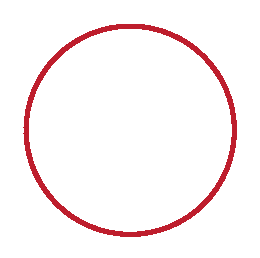
\includegraphics[trim=0cm 0cm 0cm 0cm,clip,scale=0.50]{images/projectivelinesdisk1.pdf}
	\end{minipage}\\
	\begin{minipage}{0.77\textwidth}
	\begin{enumerate}[resume=proj]
			\item Le \textit{rette} con equazione $ax+by=0$, ovvero ai \textit{piani perpendicolari} in $\realset^3$ passanti per le rette con quell'equazione $ax+by=0$:  sul modello piano corrisponde a \textbf{diametri colleganti due punti} sul bordo.
		\end{enumerate}
	\end{minipage}
\begin{minipage}{0.32\textwidth}
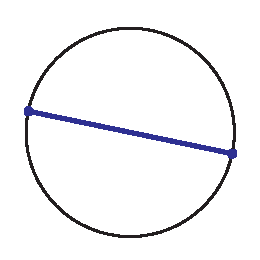
\includegraphics[trim=0cm 0cm 0cm 0cm,clip,scale=0.50]{images/projectivelinesdisk2.pdf}
\end{minipage}\\
\begin{minipage}{0.77\textwidth}
	\begin{enumerate}[resume=proj]
			\item Nel caso generale $ax+by+cz=0$, proiettando l'\textit{arco di cerchio massimo} viene un \textbf{arco di ellisse} in $D$.
		\end{enumerate}
	\end{minipage}
	\begin{minipage}{0.32\textwidth}
		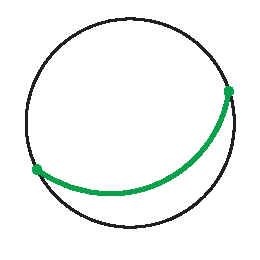
\includegraphics[trim=0cm 0cm 0cm 0cm,clip,scale=0.50]{images/projectivelinesdisk3.pdf}
	\end{minipage}
	\end{itemize}
\vspace{-3mm}
\end{examples}
\section{Operazioni con i sottospazi}
Se $W_1,\ W_2\subseteq V$ sono sottospazi vettoriali, allora $W_1\cap W_2$ è un sottospazio vettoriale e si ha che l'\textbf{intersezione}\index{sottospazio!intersezione} dei corrispettivi spazi proiettivi è ancora un sottospazio proiettivo.
\begin{equation*}
	\proj{W_1\cap W_2}=\proj{W_1}\cap\proj{W_2}
\end{equation*}
\vspace{-6mm}
\begin{observe}
	Si ha:
	\begin{equation*}
		\proj{W_1}\cap\proj{W_2}=\emptyset\iff W_1\cap W_2=\left\{0\right\}
	\end{equation*}
In tal caso diciamo che i due sottospazi sono \textbf{sghembi}\index{sottospazio!proiettivo!sghembo} o \textbf{disgiunti}\seeonlyindex{sottospazio!proiettivo!disgiunto}{sottospazio!proiettivo!sghembo}.
\end{observe}
Come per i sottospazi vettoriali, in generale l'\textbf{unione} di due sottospazi proiettivi \textit{non} è un sottospazio proiettivo.
\begin{define}[Sottospazio generato da un sottoinsieme.]~{}\\
	Sia $S\subseteq \proj{V}$ un sottoinsieme non vuoto. Il \textbf{sottospazio generato}\index{sottospazio!proiettivo!generato} da $S$, denotato con $\left<S\right>$, è l'intersezione in $\proj{V}$ di tutti i sottospazi proiettivi contenenti $S$, ed è il più piccolo sottospazio contenente $S$.
\end{define}
\begin{itemize}
	\item $\left<S\right>=S\iff S$ è un sottospazio proiettivo.
	\item Se $S=\left\{P_1,\ \ldots,\ P_m\right\}$ è finito, scriviamo $\left<P_1,\ \ldots,\ P_m\right>$ per il sottospazio generato da $P_1,\ \ldots,\ P_m$; se, sono linearmente indipendenti, $\dim \left<P_1,\ \ldots,\ P_m\right>=m-1$.
\end{itemize}
\begin{define}[Sottospazio somma.]~{}\\
	Dati due sottospazi proiettivi $T_1,\ T_2\subseteq \proj{V}$, cioè:
	\begin{equation*}
		T_i=\proj{W_i}\quad W_i\subseteq V,\ i=1,\ 2
	\end{equation*}
	Allora il sottospazio generato da $T_1\cup T_2$ è denotato con $T_1+T_2=\left<T_1,\ T_2\right>$ e si chiama \textbf{sottospazio somma}\index{sottospazio!somma}. In particolare, si ha:
	\begin{equation}
		\left<T_1,\ T_2\right>=\proj{W_1+W_2}
	\end{equation}
\vspace{-6mm}
\end{define}
\begin{demonstration}~{}\\
	$\includedx$$\proj{W_1+W_2}$ è un sottospazio proiettivo che contiene, in quanto $W_1\subseteq W_1+W_2,\ W_2\subseteq W_1+W_2$ vettorialmente, sia $T_1=\proj{W_1}$ sia $T_2=\proj{W_2}$. In particolare, contiene la loro unione\footnote{Ricordiamo che non è essa un sottospazio, ma un sottoinsieme.}, dunque $\left<T_1,\ T_2\right>=\left<T_1\cup T_2\right>\subseteq \proj{W_1+W_2}$.\\
	$\includesx$Abbiamo che $T_i\subseteq \left<T_1,\ T_2\right>=\proj{U}$, con $U$ un sottospazio vettoriale di $V$. In particolare, si ha che $W_1,\ W_2\subseteq U$, da cui $W_1+W_2\subseteq U$. Passando allo spazio proiettivo:
	\begin{equation*}
		\left<T_1,\ T_2\right>=\proj{U}\supseteq \proj{W_1+W_2}
	\end{equation*}
\vspace{-6mm}
\end{demonstration}
\begin{proposition}[Formula di Grassmann proiettiva.]~{}\index{formula!di Grassmann proiettiva}\\
Siano $T_1,\ T_2$ sottospazi proiettivi di $\proj{V}$. Si ha:
	\begin{equation}
				\dim\left<T_1,\ T_2\right>+\dim\left(T_1\cap T_2\right)=\dim T_1+\dim T_2
	\end{equation}
\vspace{-6mm}
\end{proposition}
\begin{demonstration}
	Posti $T_i=\proj{W_i}$, con $W_i\subseteq V$ sottospazi vettoriali. Dalla \textit{formula di Grassmann vettoriale}:
	\begin{equation*}
		\dim\left(W_1+W_2\right)+\dim\left(W_1\cap W_2\right)=\dim W_1+\dim W_2
	\end{equation*}
Sottraendo $1$ a tutte le dimensioni, otteniamo le dimensioni dei corrispettivi spazi proiettivi e dunque la formula proiettiva.
\end{demonstration}
\begin{corollary}[Condizioni sulla dimensione dell'intersezione.]~{}\\
	Siano $T_1,\ T_2$ sottospazi proiettivi di $\proj{V}$ con $\dim\proj{V}=n$. Allora:
	\begin{equation}
		\dim \left(T_1\cap T_2\right)\geq \dim T_1+\dim T_2-n
	\end{equation}
In particolare $T_1\cap T_2\neq \emptyset$ se $\dim T_1+\dim T_2\geq n$.
\end{corollary}
\begin{demonstration}
	\begin{equation*}
		\dim\left(T_1\cap T_2\right)=\dim T_1+\dim T_2-\dim\left<T_1,\ T_2\right>\geq \dim T_1+\dim T_2-n
	\end{equation*}
Chiaramente, se $\dim T_1+\dim T_2\geq n$, allora $\dim \left(T_1\cap T_2\right)\geq 0$ e dunque $T_1\cap T_2\neq \emptyset$.
\end{demonstration}
\begin{example}
	Nel piano proiettivo, due rette sono \textit{sempre incidenti}. Infatti, le rette hanno dimensione $1$, mentre $\dim\proj[2]{\kamp}=2$, dunque vale $1+1\leq 2$, pertanto due rette si incontrano sempre.
\end{example}
\begin{observe}
	Se consideriamo l'insieme \textit{finito di punti}, possiamo considerare lo spazio $S$ \textit{generato} da $P_1,\ \ldots,\ P_m$, cioè $S=\left<P_1,\ \ldots,\ P_m\right>$; inoltre, si ha:
	\begin{equation*}
		\dim S\leq m-1
	\end{equation*}
	Infatti, se $P_i=\left[v_i\right]$ con $v_i\in V$, allora:
	\begin{equation*}
		S=\underbrace{\proj{\lin{v_1,\ \ldots,\ v_m}}}_{\dim \mathcal{L} \leq m}
	\end{equation*}
\vspace{-3mm}
\end{observe}
\section{Punti linearmente indipendenti e in posizione generale}
\begin{define}[Punti linearmente indipendenti.]~{}\\
	Siano $P_1,\ \ldots, P_m\in\proj{V}$. Diciamo che i punti $P_1,\ \ldots,\ P_m$ sono \textbf{linearmente indipendenti}\index{linearmente indipendenti} se, scelti $v_1,\ \ldots,\ v_m\in V\setminus\left\{0\right\}$ tali che $P_i=\left[v_i\right]\ \forall i$, i vettori $v_1,\ \ldots,\ v_m$ sono \textit{linearmente indipendenti} in $V$.\\
	Se così non è, diciamo che $P_1,\ \ldots, P_m$ sono linearmente dipendenti.
\end{define}
\begin{observes}~{}
	\begin{itemize}
		\item La definizione è \textit{ben posta}. Dati $\lambda_1,\ \ldots,\ \lambda_m\in\kamp\setminus\left\{0\right\}$, si ha che:
		\begin{equation*}
			v_1,\ \ldots,\ v_m\text{ sono indipendenti}\iff\lambda_1 v_1,\ \ldots,\ \lambda_m v_m\text{ sono indipendenti.}
		\end{equation*}
		\item Se $\dim \proj{V}=n$, $\proj{V}$ contiene al più $n+1$ punti indipendenti.
		\item $P_1,\ \ldots,\ P_m$ sono indipendenti se e solo se $\dim\left<P_1,\ \ldots,\ P_m\right>=m-1$.
	\end{itemize}
\end{observes}
\begin{examples}~{}
	\begin{itemize}
		\item \textit{Due} punti $P,\ Q$ sono indipendenti se e solo se $P\neq Q$. Infatti, se $P=\left[v\right]$ e $Q=\left[w\right]$, allora:
		\begin{equation*}
			P\text{ e }Q\text{ sono indipendenti}\iff v\text{ e }w\text{ sono indipendenti}\iff v\nsim w\iff P\neq Q
		\end{equation*}
		In tal caso $\left<P,\ Q\right>$ è l'unico \textit{retta} contenente $P$ e $Q$, che indicheremo anche con $\overline{PQ}$.
		\item \textit{Tre} punti $P_1,\ P_2,\ P_3$ sono indipendenti se e solo se sono \textit{distinti} e \textit{non} sono \textit{allineati}, cioè appartenenti alla stessa retta. In tal caso $\left<P_1,\ P_2,\ P_3\right>$ è l'unico \textit{piano} contenente i tre punti.
	\end{itemize}
\vspace{-3mm}
\end{examples}
\begin{define}[Punti in posizione generale.]~{}\\
	Dati dei punti $P_1,\ \ldots,\ P_m\in\proj{V}$, diciamo che sono \textbf{in posizione generale}\index{in posizione generale}\index{posizione generale} se vale una delle due condizioni seguenti:
	\begin{itemize}
		\item $m\leq n+1$ e i punti sono \textit{linearmente indipendenti}.
		\item $m>n+1$ e ogni scelta di $n+1$ punti tra loro sono linearmente indipendenti.
	\end{itemize}
\vspace{-3mm}
\end{define}
\begin{example}~{}
		\begin{itemize}
		\item Se $n=1$, cioè $\proj{V}$ è una \textit{retta proiettiva}, allora $P_1,\ \ldots,\ P_m$ sono in posizione generale se e solo se $P_1,\ \ldots,\ P_m$ sono \textit{tutti distinti}.
		\item Se $n=2$, cioè $\proj{V}$ è una \textit{piano proiettivo}, allora $P_1,\ \ldots,\ P_m$ sono in posizione generale se e solo se $P_1,\ \ldots,\ P_m$ sono a $3$ a $3$ \textit{non} allineati.
	\end{itemize}
\vspace{-3mm}
\end{example}
\subsection{Impratichiamoci! Punti linearmente indipendenti}
\begin{exercise}\textsc{F.F.P., 2.1.}\\
	Si mostri che i punti del piano proiettivo reale:
	\begin{equation*}
		\left(\frac{1}{2}\colon 1 \colon 1\right)\quad \left(1\colon \frac{1}{3} \colon \frac{4}{3}\right)\quad \left(2\colon -1 \colon 2\right)
	\end{equation*}
Sono allineati, e si determini un'equazione della retta che li contiene.
\end{exercise}
\begin{solution}
	Per verificare che i $3$ punti sono allineati, dobbiamo verificare che i corrispondenti vettori di $\realset^3$ sono dipendenti. Riscriviamo i seguenti punti per facilitarci i calcoli:
\begin{equation*}
	\left(\frac{1}{2}\colon 1 \colon 1\right)=\left(1\colon 2 \colon 2\right)\quad \left(1\colon \frac{1}{3} \colon \frac{4}{3}\right)=\left(3\colon 1 \colon 4\right)
\end{equation*}
Verifichiamolo la dipendenza con il determinante.
	\begin{equation*}
		\det\left|\begin{array}{ccc}
			1 & 2 & 2\\
			3 & 1 & 4\\
			2 & -1 & 2
		\end{array}\right|=0
	\end{equation*}
L'equazione della retta è data dall'equazione del piano vettoriale in $\realset^3$ generate da $2$ dei $3$ vettori:
\begin{equation*}
	0=\left|\begin{array}{ccc}
		x_0 & x_1 & x_2\\
		1 & 2 & 2\\
		3 & 1 & 4
	\end{array}\right|=x_0\left(8-2\right)-x_1\left(4-6\right)+x_2\left(1-6\right)=6x_0+2x_1-5x_2
\end{equation*}
Verifichiamo che contenga anche il terzo:
\begin{equation*}
	6\cdot 2 + 2\cdot \left(-1\right) -5\cdot 2=0
\end{equation*}
\vspace{-6mm}
\end{solution}
\section{Rappresentazione parametrica di un sottospazio proiettivo}
Sia $S\subseteq\proj{V}$ un sottospazio proiettivo di dimensione $m$. Allora esistono sempre $m+1$ punti $P_0,\ \ldots,\ P_m\in S$ linearmente indipendenti che generano $S$. Infatti, se $S=\proj{W}$ con $W\subseteq V$ sottospazio vettoriale di dimensione $m+1$, possiamo scegliere una base $\left\{w_0,\ \ldots,\ w_m\right\}$ di $W$ tale per cui:
\begin{equation*}
	P_i=\left[w_i\right]\in S
\end{equation*}
Sono linearmente indipendenti (perché lo sono i vettori della base) e generano $S$.\\
Allora, tutti e soli i punti di $S$ sono della forma:
\begin{equation*}
	\left[\lambda_0 w_0+\ldots+\lambda_m w_m\right]\quad \lambda_0,\ \ldots,\ \lambda_m\in\kamp
\end{equation*}
Supponiamo ora di aver fissato una base $\left\{e_0,\ \ldots,\ e_n\right\}$ di $V$ e quindi di aver considerato il corrispondente \textit{riferimento proiettivo}. In coordinate vettoriali di $V$, un punto di $W$ è $x=\left(x_0,\ \ldots,\ x_n\right)$ se e solo se:
\begin{equation*}
	x=x_0e_0+\ldots+x_ne_n=\lambda_0 w_0+\ldots+\lambda_m w_m
\end{equation*}
Il punto $P_i$ in $V$ avrà coordinate $\left(P_{0,i},\ \ldots,\ P_{n,i}\right)\ \forall i=1,\ \ldots,\ m$, dunque il generico vettore $x$ di $W$ è espresso da:
\begin{equation}
	\begin{cases}
		x_0=\lambda_0 P_{0,0}+\lambda_1P_{0,1}+\ldots+\lambda_mP_{0,m}\\
		\vdots\\
		x_n=\lambda_0 P_{n,0}+\lambda_1P_{n,1}+\ldots+\lambda_mP_{n,m}
	\end{cases}
\end{equation}
Anche i punti di $S$ sono date da queste coordinate, dunque questa viene definita la \textbf{rappresentazione parametrica}\index{rappresentazione!parametrica} del sottospazio $S$, con $\left(\lambda_0\colon\ldots\colon\lambda_m\right)$ le coordinate omogenee di $\proj{W}$ date dalla base $\left\{w_0,\ \ldots,\ w_m\right\}$.
\begin{example}
	In $\proj[3]{\realset}$ consideriamo i punti:
	\begin{equation*}
		A=\left(1\colon 0\colon -1\colon 4\right)\quad B=\left(2\colon 3\colon 0\colon 5\right)
	\end{equation*}
Allora, la rappresentazione parametrica del sottospazio $S$ con $\left(\lambda\colon \mu\right)$ è:
\begin{equation*}
	\begin{cases}
		x_0=\lambda+2\mu\\
		x_1=3\mu\\
		x_2=-\lambda\\
		x_3=4\lambda-5\mu
	\end{cases}
\end{equation*}
\vspace{-6mm}
\end{example}
\subsection{Coordinate proiettive e punti in posizione generale}
\begin{observe}
	Sia $\proj{V}$ con un riferimento proiettivo fissato. Consideriamo i punti fondamentali $P_0,\ \ldots,\ P_n$ e il punto unità $U$.
	\begin{itemize}
		\item $P_0,\ \ldots,\ P_n,\ U$ sono $n+2$ punti.
		\item $P_0,\ \ldots,\ P_n,\ U$ sono in posizione generale: essendo $P_i=\left[e_i\right]$ con $e_0,\ \ldots,\ e_n$ base di $V$, allora $P_0,\ \ldots,\ P_n$ sono indipendenti. Se sostituiamo l'$i$-esimo punto con $U=\left[e_1+\ldots+e_n\right]$, allora:
		\begin{equation*}
			P_0,\ \ldots,\ \check{P}_i,\ \ldots,\ U
		\end{equation*}
	Sono indipendenti $\forall i=0,\ \ldots,\ n$.\footnote{Indichiamo con $\check{P}_{i}$ il punto che sostituiamo.}
	\end{itemize}
\vspace{-6mm}
\end{observe}
\begin{attention}
	Sia $\basis=\left\{e_0,\ \ldots,\ e_n\right\}$ una base che induce un \textit{riferimento proiettivo} su $\proj{V}$.\\
	Per ogni $i$ sia $\lambda_i\in\kamp\setminus\left\{0\right\}$ e consideriamo $v_i=\lambda_i e_i$. Allora $\basis'=\left\{v_0,\ \ldots,\ v_n\right\}$ è ancora una base e i \textit{punti fondamentali} del riferimento indotto da $\basis'$ sono \textit{gli stessi} del riferimento indotto da $\basis$. Infatti:
	\begin{equation*}
		\left[e_i\right]=\left[v_i\right]=P_i
	\end{equation*}
	Però i due riferimenti sono \textbf{diversi}; dato $v$ espresso nella base $\basis$:
	\begin{equation*}
		v=x_0e_0+\ldots+x_ne_n
	\end{equation*}
	La sua classe in $\proj{V}$, rispetto a $\basis$, è:
	\begin{equation*}
		\left[v\right]=\left(x_0\colon\ldots\colon x_n\right)
	\end{equation*}
	Possiamo partire dall'espressione di $v$ nella base $\basis$ a quella nella base $\basis'$, moltiplicando e dividendo ogni $e_i$ per il corrispettivo $\lambda_i$:
	\begin{equation*}
		v=\frac{x_0}{\lambda_0}\left(\lambda_0e_0\right)+\ldots+\frac{x_n}{\lambda_n}\left(\lambda_ne_n\right)=\frac{x_0}{\lambda_0}v_0+\ldots+\frac{x_n}{\lambda_n}v_n
	\end{equation*}
	Passiamo dunque alla base $\basis'$ alla classe in $\proj{\kamp}$:
	\begin{equation*}
		\left[v\right]=\left(\frac{x_0}{\lambda_0}\colon\ldots\colon\right)
	\end{equation*}
	Notiamo che effettivamente il punto $\left[v\right]$ non cambia, ma i riferimenti \textit{non} sono multipli e quindi sono diversi!
	\begin{itemize}
		\item \textit{Conoscere} i punti fondamentali \textit{non basta} a determinare la base $\basis$.
		\item Riferimenti proiettivi \textit{diversi} possono avere gli \textit{stessi} punti fondamentali.
	\end{itemize}
\end{attention}
\begin{observe}\label{puntigeneraleindipendentiosserva}
	Supponiamo di avere $n+2$ punti $P_0,\ \ldots,\ P_{n+1}$ in $\proj{V}$, cioè $\forall i=0,\ \ldots,\ n+1\ \exists v_i\in V\ \colon P_i=\left[v_i\right]$. Allora:
	\begin{gather*}
		P_0,\ \ldots,\ P_{n+1}\text{ sono in posizione generale}\iff v_0,\ \ldots,\ v_n\text{ sono indipendenti e}\\
		v_{n+1}=a_0v_0+\ldots+a_nv_n\text{ con }a_i\neq 0\ \forall i=0,\ \ldots,\ n
	\end{gather*}
Infatti, se $v_0,\ \ldots,\ v_n$ è una base (in quanto sono indipendenti), $v_0,\ \ldots,\ \check{v_i},\ \ldots,\ v_n,\ v_{n+1}$ sono indipendenti se e solo se $a_i\neq 0$.
\end{observe}
\begin{theorema}[Esistenza di una base dati $n+2$ punti in posizione generale.]~{}\label{puntiposizionegeneraleesistenzabase}\\
	Sia $\proj{V}$ di dimensione $n$. Dati $n+2$ punti $P_0,\ \ldots,\ P_{n+1}$ in \textit{posizione generale}, esiste una base $\basis=\left\{e_0,\ \ldots,\ e_n\right\}$ di $V$ tale che:
	\begin{equation}
		P_0=\left[e_0\right],\ \ldots,\ P_n=\left[e_n\right],\ P_{n+1}=\left[e_0+\ldots+e_n\right]
	\end{equation}
Inoltre, se $\basis'=\left\{f_0,\ \ldots,\ f_n\right\}$ è un'altra base di $V$ che soddisfa la condizione sopra, allora $\basis'$ è proporzionale a $\basis$, cioè $\exists\lambda\in\kamp\setminus\left\{0\right\}\ \colon f_i=\lambda e_i\ \forall i=0,\ \ldots,\ n$.
\end{theorema}
\begin{demonstration}
	Sia $P_i=\left[v_i\right]$ al variare di $i=0,\ \ldots,\ n+1$. I punti $P_0,\ \ldots,\ P_n$ sono indipendenti\footnote{Perché se $n+2$ punti sono in posizione generale, presi $n+1$ punti fra di loro sono indipendenti.}, dunque per definizione $v_0,\ \ldots,\ v_n$ è una base di $V$. Definiamo:
	\begin{equation*}
		v_{n+1}=\lambda_0v_0+\ldots+\lambda_nv_n\quad \lambda_i\in\kamp
	\end{equation*}
	Ma allora, per l'osservazione precedente, $\lambda_i\neq 0\ \forall i$ perché i punti sono in posizione generale.\\
	Consideriamo $e_0=\lambda_0v_0,\ e_1=\lambda_1v_1,\ \ldots,\ e_n=\lambda_nv_n$. Si ha che $\basis=\left\{e_0,\ \ldots,\ e_n\right\}$ è una base di $V$ perché $\lambda_i\neq 0$\ $\forall i$. Segue che:
	\begin{gather*}
		\left[e_i\right]=\left[v_i\right]=P_i\ \forall i=0,\ \ldots,\ n\\
		\left[e_0+\ldots+e_n\right]=\left[\lambda_0v_0+\ldots+\lambda_nv_n\right]=\left[v_{n+1}\right]=P_{n+1}
	\end{gather*}
Adesso, sia $\basis'=\left\{f_0,\ \ldots,\ f_n\right\}$ come da ipotesi. Allora $\left[f_i\right]=P_i=\left[e_i\right]\ \forall i=0,\ \ldots,\ n$, cioè $\exists \mu_i\in\kamp\setminus\left\{0\right\}\ \colon f_i=\mu_i e_i\ \forall i=0,\ \ldots, n$. Inoltre, soddisfa anche $\left[f_0+\ldots+f_n\right]=P_{n+1}$, pertanto:
\begin{equation*}
	\left[f_0+\ldots+f_n\right]=\left[e_0+\ldots+e_n\right]
\end{equation*}
In altre parole, $\exists \mu\in\kamp\setminus\left\{0\right\}$ tale che:
\begin{equation*}
	\begin{array}{ccc}
		f_0+\ldots+f_n&=&\mu\left(e_0+\ldots+e_n\right)\\
		\shortparallel&&\\
		\mu_0e_0+\ldots+\mu_ne_n&&
	\end{array}
\end{equation*}
$e_0,\ \ldots,\ e_n$ è una base: per l'unicità della scrittura deve essere $\mu=\mu_0=\ldots=\mu_n$, cioè $f_i=\mu e_i\ \forall i=0,\ \ldots,\ n$.
\end{demonstration}
\section{Trasformazioni proiettive}
\begin{define}[Trasformazione proiettiva e proiettività.]~{}\\
	Un'applicazione $\funz{f}{\proj{V}}{\proj{V'}}$ tra spazi proiettivi si dice \textbf{trasformazione proiettiva}\index{trasformazione!proiettiva} o \textbf{isomorfismo proiettivo}\seeonlyindex{isomorfismo!proiettivo}{trasformazione!proiettiva} se $\exists \funz{\phi}{V}{V'}$ isomorfismo che induce un altro isomorfismo lineare:
	\begin{equation}
		\begin{tikzcd}
			\widetilde{\phi}\ \colon\\
		\end{tikzcd}
			\funztot{\ }{\proj{V}}{\proj{V'}}{\left[v\right]}{\left[\phi\left(v\right)\right]}
	\end{equation}
	Tale per cui $f=\widetilde{\phi}$.\\
	Se $V=V'$, diciamo che $f$ è una \textbf{proiettività}\index{proiettività} di $\proj{V}$.
\end{define}
\begin{demonstration}~{}
	\begin{itemize}
		\item $\widetilde{\phi}$ \textbf{è ben definita}:
		\begin{enumerate}
			\item $\phi\left(v\right)\neq 0$ perché $v\neq 0$ e $\phi$ è iniettiva, pertanto $\ker\phi=\left\{0\right\}$ e dunque l'unico vettore mappato a $0$ tramite $\phi$ è solo $0$.
			\item Se $\left[v\right]=\left[w\right]$, allora $w\sim v$, cioè $w=\lambda v$ con $\lambda\in\kamp\setminus\left\{0\right\}$; segue che per linearità di $\phi$ vale $\phi\left(w\right)=\lambda \phi\left(v\right)\implies \left[\phi\left(w\right)\right]=\left[\phi\left(v\right)\right]$
		\end{enumerate}
		\item $\widetilde{\phi}$ \textbf{è iniettiva}: se $\widetilde{\phi}\left(\left[v\right]\right)=\widetilde{\phi}\left(\left[w\right]\right)$, allora
		\begin{equation*}
			\left[\phi\left(v\right)\right]=\left[\phi\left(w\right)\right]\implies\exists\lambda\in\kamp\setminus\left\{0\right\}\ \colon\phi\left(w\right)=\lambda\phi\left(v\right)=\phi\left(\lambda v\right)
		\end{equation*}
	Poiché $\phi$ è iniettiva, segue che $w=\lambda v$ e dunque $\left[v\right]=\left[w\right]$.
		\item $\widetilde{\phi}$ \textbf{è suriettiva}: infatti, se $\left[w\right]\in\proj{V'}$, essendo $\phi$ suriettiva esiste un vettore $v$ tale che $w=\phi\left(v\right)$. Segue che $\left[w\right]=\left[\phi\left(v\right)\right]=\phi\left(\left[v\right]\right)$.
	\end{itemize}
\vspace{-3mm}
\end{demonstration}
Dato che spazi \textit{vettoriali} della \textit{stessa dimensione} sono sempre \textit{isomorfi}, due spazi \textit{proiettivi} della \textit{stessa dimensione} sono sempre \textit{isomorfi} e $\proj{V}$ è sempre isomorfo a $\proj[n]{\kamp}$, con $\dim V=n+1$.
\begin{lemming}[Uguaglianza di proiettività.]~{}\\
	Siano $\funz{\phi,\ \psi}{V}{V'}$ isomorfismi. Allora:
	\begin{equation}
		\widetilde{\phi}=\widetilde{\psi}\iff\exists\lambda\in\kamp\setminus\left\{0\right\}\ \colon\psi=\lambda\phi
	\end{equation}
\vspace{-6mm}
\end{lemming}
\begin{demonstration}~{}\\
$\impliessx$Se $v\in\kamp\setminus\left\{0\right\}$, allora $\psi\left(v\right)=\lambda\phi\left(v\right)$. Segue:
\begin{equation*}
	\implies \widetilde{\phi}\left(\left[v\right]\right)=\left[\phi\left(v\right)\right]=\left[\psi\left(v\right)\right]=\widetilde{\psi}\left(\left[v\right]\right)
\end{equation*}
$\impliesdx$Sia $h\coloneqq \funz{\psi^{-1}\circ \phi}{V}{V}$ automorfismo. Vogliamo mostrare che $h=\lambda Id_V$ con $\lambda\in\kamp\setminus\left\{0\right\}$. Se $v\in V\setminus\left\{0\right\}$, abbiamo:
\begin{equation*}
	\begin{array}{c}
\begin{array}{ccc}
	\widetilde{\phi}\left(\left[v\right]\right)&=&\widetilde{\psi}\left(\left[v\right]\right)\\
	\shortparallel&&\shortparallel\\
	\left[\phi\left(v\right)\right]&&\left[\psi\left(v\right)\right]
\end{array}
\implies \lambda_v\in\kamp\setminus\left\{0\right\}\ \colon \phi\left(v\right)=\lambda_v\psi\left(v\right)
\implies h\left(v\right)=\psi^{-1}\left(\phi\left(v\right)\right)=\lambda_v v
\end{array}
\end{equation*}
Segue che $v$ è autovettore di $h\ \forall v\in V\setminus\left\{0\right\}$, in particolare ogni vettore non nullo è autovettore di $h$. Segue che $h$ è diagonalizzabile e ha un unico autovalore $\lambda$. Infatti, presi $\lambda_1$ e $\lambda_2$, si avrebbero i seguenti autovalori indipendenti:
\begin{equation*}
	v_1\in V_{\lambda_1}\setminus\left\{0\right\}\qquad v_2\in V_{\lambda_2}\setminus\left\{0\right\}
\end{equation*}
E considerato che:
\begin{equation*}
	\begin{array}{l}
		h\left(v_1\right)=\lambda_1 v_1\\
		h\left(v_2\right)=\lambda_2 v_2\\
		h\left(v_1+v_2\right)=\lambda\left(v_1+v_2\right)\\
		h\left(v_1+v_2\right)=h\left(v_1\right)+h\left(v_2\right)\\
	\end{array}
	\implies \lambda\left(v_1+v_2\right)=\lambda_1 v_1+\lambda_2 v_2
\end{equation*}
Da cui segue, in quanto $v_1,\ v_2,\ v_1+v_2\neq 0$, che $\lambda=\lambda_1=\lambda_2$ e quindi è unico.\\
Allora, $h=\lambda Id_{V}$ e pertanto $\phi=\lambda \psi$.
\end{demonstration}
\subsection{Gruppo lineare proiettivo}
\begin{observe}
	Consideriamo $\proj{V}$ e l'insieme delle proiettività $\funz{\ }{\proj{V}}{\proj{V}}$.
	\begin{itemize}
		\item La \textit{composizione} di proiettività è una \textit{proiettività} (banalmente \textit{indotta} dalla composizione delle applicazioni lineari).
		\item Poiché $Id_{\proj{V}}=\widetilde{Id_V}\implies$ L'identità $Id_{\proj{V}}$ è una \textit{proiettività}.
		\item Se $\widetilde{\phi}\! \funz{\! }{\proj{V}}{\proj{V}}$, allora $\widetilde{\phi^{-1}}=\funz{f^{-1}}{\proj{V}}{\proj{V}}$. In altre parole, l'\textit{inversa} di una proiettività è ancora una proiettività.
	\end{itemize}
L'insieme delle proiettività risulta un \textbf{gruppo} rispetto alla \textit{composizione}.
\end{observe}
\begin{define}[Gruppo lineare proiettivo.]~{}\\
Il \textbf{gruppo lineare proiettivo}\index{gruppo!lineare proiettivo} $\projgl{V}$ è il gruppo delle proiettività dello spazio vettoriale $V$ con operazione la composizione di proiettività ed elemento neutro $Id_{\proj{V}}$.
\vspace{-3mm}
\end{define}
\subsubsection{Descrizione matriciale del gruppo lineare proiettivo}
Consideriamo gli isomorfismi $\funz{\ }{\kamp^{n+1}}{\kamp^{n+1}}$: sappiamo che la matrice associata agli isomorfismi è una matrice invertibile, cioè si ha una \textit{isomorfismo di gruppi} fra l'insieme degli isomorfismi in $\kamp^{n+1}$ al \textit{gruppo generale lineare} $\gl\left(n+1,\ \kamp\right)$:
\begin{equation*}
	\left\{\text{isomorfismi}\funz{\ }{\kamp^{n+1}}{\kamp^{n+1}}\right\}\leftrightarrow\gl\left(n+1,\ \kamp\right)
\end{equation*}
E con il gruppo lineare proiettivo si può fare? Consideriamo:
\begin{equation}
	\funztot{\oldphi}{\gl\left(n+1,\ \kamp\right)}{\projgl[n+1]{\kamp}}{\phi_A}{\widetilde{\phi}_A}
\end{equation}
 $\oldphi$ è \textit{omomorfismo} di gruppi \textit{suriettivo}, ma non iniettivo. Infatti, il nucleo non è \textit{triviale}:
 \begin{equation*}
 	\ker \oldphi=\left\{\phi_A\mid \phi_A=Id_{\proj[n]{\kamp}}=\widetilde{Id}_{\kamp^{n+1}}\right\}=\left\{\phi_A\mid \phi=\lambda I,\ \lambda\in\kamp\setminus\left\{0\right\}\right\}=\left\{\phi_A\mid A=\lambda I,\ \lambda\in\kamp\setminus\left\{0\right\}\right\}
 \end{equation*}
Tuttavia, possiamo per il Teorema dell'isomorfismo per i gruppi considerare il seguente diagramma commutativo:
\[\begin{tikzcd}
	{\gl\left(n+1,\ \kamp\right)} & {\projgl[n+1]{\kamp}} \\
	{\frac{\gl\left(n+1,\ \kamp\right)}{\left\{\lambda I\ \mid\ \lambda\in\kamp\setminus\left\{0\right\}\right\}}}
	\arrow["{\pi}"', from=1-1, to=2-1]
	\arrow["{\exists \overline f}"', from=2-1, to=1-2, dashed]
	\arrow["{\oldphi}", from=1-1, to=1-2]
\end{tikzcd}\]
E si ha pertanto l'isomorfismo:
\begin{equation*}
	\projgl[n+1]{\kamp}\cong \frac{\gl\left(n+1,\ \kamp\right)}{\left\{\lambda I\mid\lambda\in\kamp\setminus\left\{0\right\}\right\}}=\frac{\gl\left(n+1,\ \kamp\right)}{\left\{\lambda I\right\}}
\end{equation*}
Si può anche considerare l'isomorfismo tra $\left\{\lambda I\mid\lambda\in\kamp\setminus\left\{0\right\}\right\}$ e $\kamp\setminus\left\{0\right\}$, e riscrivere l'isomorfismo trovato come:
\begin{equation*}
	\projgl[n+1]{\kamp}\cong \frac{\gl\left(n+1,\ \kamp\right)}{\kamp\setminus\left\{0\right\}}
\end{equation*}

\begin{example}
	Consideriamo la seguente proiettività della \textit{retta proiettiva} $\proj[1]{\realset}$:
	\begin{equation*}
		\funztot{f}{\proj[1]{\realset}}{\proj[1]{\realset}}{\left(x_0\colon x_1\right)}{\left(ax_0+bx_1\colon cx_0+dx_1\right)}
	\end{equation*}
	Considerato il gruppo lineare proiettivo $\proj[2]{\realset}=\frac{\gl\left(2,\ \realset\right)}{\left\{\lambda I\right\}}$, per definizione di $f$ si ha $f=\widetilde{\phi}$. In particolare, la matrice associata a $\phi$ è:
	\begin{equation*}
		A=\left(\begin{array}{cc}
			a & b\\
			c & d
		\end{array}\right)
	\end{equation*}
	E dunque possiamo scrivere l'applicazione lineare $\phi$ come:
	\begin{equation*}
		\funztot{f}{\realset^2}{\realset^2}{\left(\begin{array}{c}
				x_0 \\
				x_1
			\end{array}\right)}{A\left(\begin{array}{c}
				x_0 \\
				x_1
			\end{array}\right)}
	\end{equation*}
	E dunque $f$ si può anche scrivere come:
	\begin{equation*}
		\funztot{f}{\projgl[2]{\kamp}}{\proj[1]{\realset}}{\left[v\right]}{\left[Av\right]}
	\end{equation*}
	Notiamo che se la matrice associata a $\phi$ fosse $2A$, per \textit{proporzionalità} si avrebbe comunque la proiettività $f$. In modo analogo, $\lambda A$ con $\lambda\in\realset\setminus\left\{0\right\}$ induce la \textit{stessa proiettività} $f$ di $A$.
	\vspace{-3mm}
\end{example}
\subsection{Altri aspetti delle trasformazioni proiettive}
\begin{observe}
	Se $f$ è una proiettività di $\proj{V}$ e $S\subseteq \proj{V}$ un sottospazio proiettivo, allora $f\left(S\right)$ è ancora un sottospazio proiettivo della stessa dimensione di $S$. Se $S=\proj{W}$ e consideriamo per definizione $f=\widetilde{\phi}$ con $\funz{\phi}{V}{V}$, allora:
	\begin{equation*}
		\forall \left[v\right]\in S\ f\left(\left[v\right]\right)=\widetilde{\phi}\left(\left[v\right]\right)=\left[\phi\left(v\right)\right],\ \phi\left(v\right)\in W
	\end{equation*}
	\begin{equation}
		f\left(S\right)=\proj{\phi\left(W\right)}
	\end{equation}
\vspace{-6mm}
\end{observe}
\begin{define}[Proiettivamente equivalenti.]~{}\\
	Due sottoinsiemi $A,\ B$ di $\proj{V}$ si dicono \textbf{proiettivamente equivalenti}\index{proiettivamente equivalenti} se $\exists f$ proiettività di $\proj{V}$ tale che:
	\begin{equation}
		B=f\left(A\right)
	\end{equation}
\vspace{-6mm}
\end{define}
\begin{example}
	Due sottospazi proiettivi di $\proj{V}$ della \textit{stessa} dimensione sono sempre \textit{proiettivamente equivalenti}.
\end{example}
\begin{theorema}[Esistenza e unicità di una trasformazione proiettiva dati $n+2$ punti in posizione generale.]~{}\label{puntigeneralitrasformazioni}\\
Siano $\proj{V}$ e $\proj{V'}$ di dimensione $n$. Siano:
	\begin{itemize}
		\item $P_0,\ \ldots,\ P_{n+1}\in\proj{V}$ $n+2$ punti in posizione generale.
		\item $Q_0,\ \ldots,\ Q_{n+1}\in\proj{V'}$ $n+2$ punti in posizione generale.
	\end{itemize}
Allora $\exists!\funz{f}{\proj{V}}{\proj{V'}}$ trasformazione proiettiva tale che $f\left(P_i\right)=Q_i\ \forall i=0,\ \ldots,\ n+1$.\\
In particolare: se una proiettività fissa $n+2$ punti ($f\left(P_i\right)=P_i\ \forall i=0,\ \ldots,\ n+1$) in posizione generale, allora è l'identità.
\end{theorema}
\begin{demonstration}~{}
	\begin{itemize}
		\item \textbf{Esistenza}: Siano, $\forall i$:
		\begin{itemize}
			\item $P_i=\left[v_i\right]\ v_i\in V$.
			\item $Q_i=\left[w_i\right]\ w_i\in V'$.
		\end{itemize}
	Sappiamo, dall'osservazione a pag. \pageref{puntigeneraleindipendentiosserva}, che:
	\begin{itemize}
		\item $v_0,\ \ldots,\ v_n$ è base di $V$, con $v_{n+1}=\lambda_0v_0+\ldots+\lambda_n v_n$ con $\lambda_i\neq 0\ \forall i$.
		\item $w_0,\ \ldots,\ w_n$ è base di $V'$, con $w_{n+1}=\mu_0w_0+\ldots+\mu_n w_n$ con $\mu_i\neq 0\ \forall i$.
	\end{itemize}
		A meno di cambiare i rappresentanti dei punti, possiamo supporre senza perdita di generalità che $\lambda_i=\mu_i=1$. Si ha dunque:
		\begin{gather*}
			v_{n+1}=v_0+\ldots+v_n\\
			w_{n+1}=w_0+\ldots+w_n
		\end{gather*}
	Sia $\funz{\phi}{V}{V'}$ l'applicazione lineare tale per cui $\phi\left(v_i\right)=w_i\ \forall i=0,\ \ldots,\ n$. Per linearità:
	\begin{equation*}
		\phi\left(v_{n+1}\right)=\phi\left(v_0+\ldots+v_n\right)=\phi\left(v_0\right)+\ldots+\phi\left(v_n\right)=w_0+\ldots+w_n=w_{n+1}
	\end{equation*}
Poiché $\im \phi$ contiene una base per costruzione, $\phi$ è suriettiva. In particolare, essendo endomorfismo ($\dim V=\dim V'$), $\phi$ è anche \textit{isomorfismo}.\\
Allora $f\coloneqq\widetilde{\phi}\funz{\ }{\proj{V}}{\proj{V'}}$ è una \textit{trasformazione proiettiva} e:
\begin{equation*}
	f\left(P_i\right)=f\left(\left[v_i\right]\right)=\left[\phi\left(v_i\right)\right]=\left[w_i\right]=Q_i\ \forall i=0,\ \ldots,\ n+1
\end{equation*}
\item \textbf{Unicità}: sia $\funz{g}{\proj{V}}{\proj{V'}}$ un'altra trasformazione proiettiva tale che $g\left(P_i\right)=Q_i\ \forall i=0,\ \ldots,\ n+1$. Per definizione, esiste $\funz{\psi}{V}{V'}$ isomorfismo per cui $g=\widetilde{\psi}$ e:
\begin{equation*}
	\left[\psi\left(v_i\right)\right]=\left[w_i\right]\ \forall i
\end{equation*}
Si ha che $\exists a_i\in\kamp\setminus\left\{0\right\}$ tale che $\psi\left(v_i\right)=a_iw_i$. Allora:
\begin{equation*}
	\begin{array}{ccccc}
		a_{n+1}w_{n+1}&=&\psi\left(v_{n+1}\right)&=&\psi\left(v_0+\ldots+v_n\right)\\
		\shortparallel&&&&\shortparallel\\
		a_{n+1}\left(w_0+\ldots+w_n\right)&&&&\psi\left(v_0\right)+\ldots+\psi\left(v_n\right)\\
		\shortparallel&&&&\shortparallel\\
		a_{n+1}w_0+\ldots+a_{n+1}w_n&&&&a_0w_0+\ldots+a_nw_n
	\end{array}
\end{equation*}
Poiché $w_0,\ \ldots,\ w_n$ è base, la scrittura è unica. Segue che $a_0=a_1=\ldots=a_{n+1}=a$. Allora:
\begin{equation*}
	\begin{array}{l}
		\psi\left(v_i\right)=aw_i=a\phi\left(v_i\right)\\
		\implies \psi=a\phi\\
		\implies g=\widetilde{\psi}=\widetilde{\phi}=f
	\end{array}
\end{equation*}
	\end{itemize}
\vspace{-6mm}
\end{demonstration}
\begin{examples}~{}
	\begin{itemize}
		\item In una \textit{retta proiettiva} ($\dim 1$), una proiettività è determinata dalle immagini di $3$ \textit{punti distinti}, dato che è equivalente alla condizione di ‘‘\textit{punti in posizione generale}''.
		\item In un \textit{piano proiettivo} ($\dim 2$), una proiettività è determinata dalle \textit{immagini} di $4$ punti, a $3$ a $3$ \textit{non allineati}.
		\item Se $A,\ B\subseteq \proj{V}$ sono insiemi finiti, ciascuno contenente $k$ punti in posizione generale, con $k\leq n+2$, allora $A$ e $B$ sono sempre proiettivamente equivalenti.
	\end{itemize}
\vspace{-3mm}
\end{examples}
\begin{example}
	Approfondiamo l'ultimo esempio. In $\proj[2]{\kamp}$ ($\dim 2$), si prenda $A=\left\{P_1,\ P_2\right\},\ B=\left\{Q_1,\ Q_2\right\}$ con $P_1\neq P_2$, $Q_1\neq Q_2$. Ho due punti distinti sia in $A$ e $B$, dunque esiste sempre una proiettività $\funz{f}{\proj[2]{\ }}{\proj[2]{\ }}$ tale che $f\left(A\right)=B$.\\
	Se invece $A$ e $B$ contengono $3$ punti, se i $3$ punti in $A$ \textit{sono allineati} mentre i $3$ punti in $B$ \textit{non} lo sono, allora $A$ e $B$ \textit{non} sono proiettivamente equivalenti.
\end{example}
\subsection{Trasformazioni proiettive in coordinate}
Supponiamo di avere fissato dei \textit{riferimenti proiettivi} su $\proj{V}$ e $\proj{V'}$, dati da delle basi $\basis$ di $V$ e $\basis'$ di $V'$, e sia $\funz{f}{\proj{V}}{\proj{V'}}$ una trasformazione proiettiva. Sappiamo che $f=\widetilde{\phi}$ con $\funz{\phi}{V}{V'}$ isomorfismo lineare.\\
Sia $A\in\gl\left(n+1,\ \kamp\right)$ la matrice associata a $\phi$ rispetto alle basi $\basis$ e $\basis'$. Abbiamo visto che $\phi$ è determinata solo a meno di multipli: chiaramente, lo stesso è vero anche per $A$.\\
Siano allora:
\begin{gather*}
	P=\left(x_0\colon\ldots\colon x_n\right)\in\proj{V}\\
	f\left(P\right)=\left(y_0\colon\ldots\colon y_n\right)\in\proj{V'}
\end{gather*}
Allora $\exists\rho\in\kamp\setminus\left\{0\right\}$ tale che $\rho y=Ax$.
\begin{observe}\textsc{Cambiamenti di coordinate.}\\
Se in $\proj{V}$ abbiamo due riferimenti proiettivi, uno dalla dalla base $\basis$, e uno dalla base $\basis'$, sia $M$ la \textit{matrice del cambiamento di base} in $V$ tale che:
\begin{equation*}
	x'=Mx
\end{equation*}
Con $x$ in coordinate rispetto alla base $\basis$ e $x'$ in coordinate rispetto alla base $\basis'$. Allora, se $P\in\proj{V}$ ha coordinate:
\begin{equation*}
	\left(x_0\colon\ldots\colon x_n\right)\text{ rispetto a }\basis\\
	\left(x_0'\colon\ldots\colon x_n'\right)\text{ rispetto a }\basis'
\end{equation*}
Esiste $\rho\in\kamp\setminus\left\{0\right\}$ tale che $\rho x'=M x$.
\end{observe}
\subsection{Punti fissi di proiettività}
\begin{define}[Punto fisso.]~{}\\
	Sia $\funz{f}{\proj{V}}{\proj{V}}$ una proiettività. Un \textbf{punto fisso}\index{punto!fisso} è un punto $P\in\proj{V}$ tale che:
	\begin{equation}
		f\left(P\right)=P
	\end{equation}
\vspace{-6mm}
\end{define}
Sia $\funz{\phi}{V}{V}$ un \textit{automorfismo} tale che $f=\widetilde{\phi}$, e sia $P=\left[v\right]$, con $v\in V\setminus\left\{0\right\}$. Allora:
\begin{equation*}
	\begin{array}{ll}
		& f\left(P\right)=\left[\phi\left(v\right)\right]=\left[v\right]\\
		\iff & \exists\lambda\in\kamp\setminus\left\{0\right\}\ \colon \phi\left(v\right)=\lambda v\\
		\iff & v\text{ è un autovettore per }\phi
	\end{array}
\end{equation*}
In particolare, $\phi$ è invertibile, dunque \textit{non} ha l'autovettore \textit{nullo}. Segue che i punti fissi di $f$ sono tutti e soli i punti $\left[v\right]$ con $v$ autovettore di $\phi$.
\begin{observes}~{}
	\begin{enumerate}
		\item Se $\kamp=\complexset$, allora ogni proiettività ha almeno un punto fisso, dato che $\phi$ ha sempre almeno un autovettore.
		\item Se $\kamp=\realset$ e $\dim\proj{V}=n$, allora $\dim V=n+1$. Il \textit{polinomio caratteristico} $C_\phi\left(t\right)\in\realset\left[t\right]$ ha grado $n+1$. Se $n$ è \textit{pari}, $\phi$ ha almeno un autovalore, dato che il polinomio caratteristico ha grado $n+1$ \textit{dispari}: infatti, o è di grado \textit{uno} (e quindi ha banalmente soluzione) oppure, in quanto si può decomporre in fattori a coefficienti reali al più di grado \textit{due}, ammetterà \textit{sempre} almeno un fattore di grado \textit{uno}.
		\item Portiamo un controesempio al caso $n$ dispari. Sia $\funztot{f}{\proj{\realset}}{\proj{\realset}}{\left(x\colon y\right)}{\left(-y\colon x\right)}$. La matrice $A$ associata a $f$ è:
		\begin{equation*}
			A=\left(\begin{array}{cc}
				0 & -1 \\
				1 & 0
			\end{array}\right)
		\end{equation*}
	Il polinomio caratteristico \textit{non} ha radici \textit{reali}:
	\begin{equation*}
		C_A\left(t\right)=\det\left(\begin{array}{cc}
			-t & -1 \\
			1 & -t
		\end{array}\right)=t^2-1
	\end{equation*}
Segue che $A$ non ha autovettori reali e pertanto $f$ \textit{non} ha punti fissi.
\item In generale, l'\textit{insieme} dei punti fissi di $\funz{f}{\proj{V}}{\proj{V}}$ è dato da:
\begin{equation*}
	\left\{\proj{V_{\lambda}}\mid\lambda\text{ autovalore di }\phi\right\}
\end{equation*}
Questo è un insieme di sottospazi proiettivi a 2 a 2 disgiunti.
 	\end{enumerate}
\end{observes}
\begin{define}[Insieme fisso.]~{}\\
	Se $S\subseteq\proj{V}$ è un sottospazio, diciamo che $S$ è \textbf{fisso} per $f$ proiettività se:
		\begin{equation}
		f\left(S\right)=S
	\end{equation}
	\vspace{-6mm}
\end{define}
\subsection{Impratichiamoci! Trasformazioni proiettive}
\begin{exercise}
	In $\proj[1]{\realset}$ determinare la proiettività $f$ tale che:
	\begin{equation*}
		f\left(2\colon 1\right)=\left(1\colon1\right)\quad f\left(1\colon 2\right)=\left(0\colon1\right)\quad
		f\left(1\colon -1\right)=\left(1\colon0\right)
	\end{equation*}
\vspace{-6mm}
\end{exercise}
\begin{solution}
Notiamo che i punti:
\begin{equation*}
	\left(2\colon 1\right)\quad\left(1\colon 2\right)\quad\left(1\colon -1\right)\text{ e }	\left(1\colon 1\right)\quad\left(0\colon 1\right)\quad\left(1\colon 0\right)
\end{equation*}
Sono distinti, dunque sono in posizione generale e la proiettività è garantita. Prendiamo la generica matrice $A=\left(\begin{array}{cc}
	a & b\\
	c & d
\end{array}\right)$ associata a $\phi$ indotta da $f$ e consideriamo $\rho y=Ax$:
\begin{equation*}
	\begin{cases}
		\rho y_0=ax_0+bx_1\\
		\rho y_1=cx_0+dx_1
	\end{cases}
\end{equation*}
Imponiamo il passaggio per $f\left(2\colon 1\right)=\left(1\colon1\right)$:
\begin{equation*}
	\begin{cases}
		\rho=1a+b\\
		\rho=2c+d
	\end{cases}\implies 2a+b=2c+d
\end{equation*}
In sostanza, \textit{eliminiamo} il parametro $\rho$ per ottenere un'equazione lineare \textit{omogenea} tra gli elementi della matrice.\\
Facciamo lo stesso con i rimanenti punti $f\left(1\colon 2\right)=\left(0\colon1\right)$ e $	f\left(1\colon -1\right)=\left(1\colon0\right)$, utilizzando rispettivamente $\mu y=Ax$ e $\alpha y=Ax$:
\begin{gather*}
	\begin{cases}
		0=a+2b\\
		\rho=c+2d
	\end{cases}\implies a+2b=0\\
	\begin{cases}
		\alpha=a-b\\
		0=c-d
	\end{cases}\implies c-d=0
\end{gather*}
Costruiamo così un sistema lineare omogeneo di $3$ equazioni in $4$ incognite $a,\ b,\ c,\ d$, con una matrice dei coefficienti di rango $3$:
\begin{equation*}
	\begin{cases}
		2a+b=2c+d\\
		a+2b=0\\
		c-d=0
	\end{cases}\implies \begin{cases}
	a=2c\\
	b=-c\\
	c=c\\
	d=c
\end{cases}\implies
A=\left(\begin{array}{cc}
	2c & -c\\
	c & c
\end{array}\right)=c\left(\begin{array}{cc}
1 & -1\\
1 & 1
\end{array}\right)
\end{equation*}
A meno di multipli, $A=\left(\begin{array}{cc}
	1 & -1\\
	1 & 1
\end{array}\right)$ è la matrice cercata. Segue dunque che la proiettività cercata è:
\begin{equation*}
	\funztot{f}{\proj[1]{\realset}}{\proj[1]{\realset}}{\left(x_0\colon x_1\right)}{\left(2x_0-x_1\colon x_0+x_1\right)}
\end{equation*}
\vspace{-3mm}
\end{solution}
\section{Geometria affine e geometria proiettiva}\label{spaziaffini}
Abbiamo già accennato all'esistenza di una relazione che intercorre fra \textit{geometria affine} e \textit{geometria proiettiva}. Diamo innanzitutto qualche richiamo dei concetti della geometria affine.
\begin{define}[Spazio affine.]~{}\\
	Sia $V$ uno spazio vettoriale di dimensione finita su un campo $\kamp$. Uno \textbf{spazio affine}\index{spazio!affine} di dimensione $n$ su $V$ (con spazio vettoriale associato $V$ di dimensione $n$ ) è un insieme $\aff{V}$ non vuoto di \textit{punti} (elementi) tale che sia data un'applicazione:
	\begin{equation*}
		\funztot{\ }{\aff{V}\times\aff{V} }{V}{\left(P,\ Q\right)}{\overrightarrow{PQ}}
	\end{equation*}
	Che alla coppia di punti $\left(P,\ Q\right)$ associa il vettore di $V$ con punto iniziale $P$ e punto finale $Q$ e tale che siano
	soddisfatti i seguenti assiomi:
	\begin{enumerate}
		\item $\forall P\in\aff{V},\ \forall v\in V$ esiste un unico punto $Q\in\aff{V}$ tale che $\overrightarrow{PQ}=v$.
		\item $\forall P,\ Q,\ R\in\aff{V}$ terna di punti di $\aff{V}$ si ha $\overrightarrow{PQ}+\overrightarrow{QR}=\overrightarrow{PR}$.
	\end{enumerate}
\end{define}
\begin{define}[Riferimento affine e coordinate affini.]~{}\\
	Un \textbf{riferimento affine}\index{riferimento!affine} $\mathcal{R} = (O,\  e_1,\  e_2,\ \ldots,\  e_n)$ sullo spazio $\aff{V}$ è assegnato fissando un punto $O\in \aff{V}$ detta \textbf{origine}\index{origine affine} ed una base $\basis = (e_1,\  e_2,\ \ldots,\  e_n)$ di $V$. Dunque, per ogni $P\in \aff{V}$ si ha la $n$-upla $(X_1,\  X_2,\ \ldots,\  X_n)$ dette \textit{coordinate affini}\index{coordinate!affini} del punto $P\in\aff{V}$ (uniche per riferimento affine fissato) tale per cui:
	\begin{equation}
		P=\overrightarrow{OV}=x_1e_1+\ldots+x_ne_n
	\end{equation}
\vspace{-6mm}			
\end{define}
Per i nostri scopi, parleremo spesso degli spazi affini di dimensione $n$ su $\kamp$.
\begin{define}[Affinità.]~{}\\
	Un'\textbf{affinità}\seeonlyindex{affinità}{trasformazione!lineare affine} o \textbf{trasformazione lineare affine}\index{trasformazione!lineare affine} di $\aff{\kamp^n}$ è un'applicazione:
	\begin{equation}
		\funz{\phi}{\aff{\kamp^n}}{\aff{\kamp^n}}
	\end{equation}
Della forma $\phi\left(x\right)=Ax+b$ con $A\in\gl\left(n,\ \kamp\right)$ un'applicazione lineare invertibile e $b$ una \textit{traslazione}.
\end{define}
\begin{define}[Sottospazio affine.]~{}\\
	Un \textbf{sottospazio affine}\index{sottospazio!affine} di $\aff{\kamp^n}$ è un \textit{traslato} di un sottospazio vettoriale $W\subseteq \kamp^n$:
	\begin{equation}
		S=W+x_0=\left\{w+x_0\mid w\in W,\ x_0\in\aff{W}\right\}
	\end{equation}
\vspace{-6mm}
\end{define}
\begin{observes}~{}
	\begin{itemize}
		\item $W$ è l'unico traslato di $S$ per l'origine ($x_0=O$) e si dice \textbf{sottospazio direttore}  di $S$\index{sottospazio!direttore}, cioè ne dà appunto la \textit{direzione}. Si definisce $\dim S\coloneqq\dim W$.
		\item Un punto in $\aff{\kamp^n}$ è un sottospazio affine di dimensione $0$ ($W=\left\{0\right\}$; dopotutto non ha particolarmente senso parlare di direzione del punto).
		\item Una \textbf{retta affine}\index{retta!affine} $r$ in $\aff{\kamp^n}$ è un sottospazio affine di $\dim 1$: $W=\lin{v}$, cioè $r$ si può individuare assegnando un punto $P\in r$ e un qualsiasi vettore $v$ \textit{parallelo} alla retta $r$.
		\item Un \textbf{piano affine}\index{piano!affine} $\pi$ in $\aff{\kamp^n}$ è un sottospazio affine di $\dim 2$: $W=\lin{v,\ w}$, cioè $\pi$ si può individuare assegnando un punto $P\in r$ e una coppia di vettori l.i. \textit{paralleli} al piano $\pi$.
		\item Un \textbf{iperpiano affine}\index{iperpiano!affine} è un sottospazio di dimensione $n-1$.
		\item Due sottospazi affini della stessa dimensione si dicono \textbf{paralleli}\index{sottospazio!affine!parallelo} se hanno lo \textit{stesso} sottospazio direttore.
	\end{itemize}
\vspace{-3mm}
\end{observes}
\begin{example}
Consideriamo $r=W+x_0$ retta affine, che ha dunque $\dim r=\dim W=1$. $W$ è la retta vettoriale in $\kamp^n$, mentre un qualunque $v\in W\setminus\left\{0\right\}$ è la \textit{direzione} della retta.
\end{example}
Un sottospazio affine $S\subseteq \kamp^n$ può essere descritto con equazioni cartesiane oppure in forma parametrica.\\
	\textbf{Equazioni cartesiane}. $S$ è visto come l'insieme delle \textit{soluzioni} del seguente sistema lineare:
	\begin{equation}
		Ax=b\qquad\left(\begin{array}{c}
			X_1\\
			\vdots\\
			X_n
		\end{array}\right)\in\aff{\kamp^{n}}
	\end{equation}
Con $b$ che descrive la traslazione dovuta a $x_0\in\aff{W}$.
In tal caso $W$ è il sottospazio vettoriale delle soluzioni del sistema lineare omogeneo associato:
\begin{equation}
	Ax=0
\end{equation}
\textbf{Forma parametrica}. Supponiamo $\dim S=\dim W=m$. Siano $v_1,\ \ldots,\ v_m\in\kamp^n$ i vettori di una base di $W$; rispetto ad una base di $\kamp^n$, e dunque rispetto ad un sistema di riferimento affine con origine $O$, essi sono espressi nelle componenti:
\begin{equation*}
	v_i=\left(V_{i,1},\ \ldots,\ V_{i,n}\right)\in\aff{\kamp^n}
\end{equation*}
Consideriamo $S=W+c$, con il punto $c=\left(C_1,\ \ldots,\ C_n\right)$ rispetto allo stesso sistema affine di prima.\\
I punti $x$ di $S$ in forma parametrica sono dati da:
\begin{equation}
	x=t_1v_1+\ldots+t_mv_m+c\quad t_1,\ \ldots,\ t_m\in\kamp
\end{equation}
Da cui otteniamo il sistema $n\times\left(m+1\right)$ seguente:
\begin{equation}
	\begin{cases}
		\begin{array}{l}
			X_1=t_1V_{1,1}+\ldots+t_mV_{m,1}+C_1\\
			\vdots\\
			X_n=t_1V_{1,n}+\ldots+t_mV_{m,n}+C_n\\			
		\end{array}
	\end{cases}
\end{equation}
\begin{example}
	La retta $r$ ($\dim W=1$) passante per $c$ con direzione $v$ è descritto parametricamente da:
\begin{equation*}
	\begin{cases}
		\begin{array}{l}
			X_1=tV_1+c_1\\
			\vdots\\
			X_n=tV_n+c_n			
		\end{array}
	\end{cases}
\end{equation*}	
\end{example}
Consideriamo ora lo \textit{spazio proiettivo numerico}:
\begin{equation*}
	\proj[n]{\ }=\proj[n]{\kamp}=\proj{\kamp^{n+1}}
\end{equation*}
E i punti in coordinate omogenee $\left(x_0\colon \ldots\colon x_n\right)$ rispetto ad un dato sistema di riferimento proiettivo.
Consideriamo il seguente sottoinsieme di $\proj[n]{\ }$:
\begin{equation}
	U_0\coloneqq \left\{P=\left(x_0\colon\ldots\colon x_n\right)\in \proj[n]{\ }\mid x_0\neq 0\right\}
\end{equation}
La condizione $x_0\neq 0$ è \textit{ben posta}; infatti, se $\lambda\in\kamp\setminus\left\{0\right\}$, allora $x_0\neq 0\iff\lambda x_0\neq 0$.\\
Consideriamo anche il suo complementare, che è l'iperpiano coordinato rispetto alla prima coordinata omogenea:
\begin{equation}
	\proj[n]{\ }\setminus U_0=H_0=\left\{P=\left(x_0\colon\ldots\colon x_n\right)\in \proj[n]{\ }\mid x_0= 0\right\}=\left\{P=\left(0\colon\ldots\colon x_n\right)\in \proj[n]{\ }\right\}
\end{equation}
Sia $P\in U_0$: allora essendo $a_0\neq 0$ si ha $P=\left(a_0\colon\ldots\colon a_n\right)=\left(1\colon\frac{a_1}{a_0}\ldots\colon \frac{a_n}{a_0}\right)$. In particolare, $\frac{a_1}{a_0},\ \ldots,\ \frac{a_n}{a_0}$ sono univocamente determinate da $P$.
\begin{example}
 Sia $\proj[2]{\realset}=\left\{\text{rette vettoriali in }\realset^3\right\}$ con punti di componenti $\left(x_0\colon x_1\colon x_2\right)$. Allora $H_0$ è una retta proiettiva in $\proj[2]{\realset}$ e risulta:
 \begin{equation*}
 	\begin{array}{ll}
 		H_0 & =\left\{P=\left(x_0\colon x_1\colon x_2\right)\in \proj[n]{\ }\mid x_0=0\right\}=\left\{P=\left(0\colon x_1\colon x_2\right)\in \proj[n]{\ }\right\} \\
 		& =\left\{\text{rette vettoriali di }\realset^3\text{ contenute nel piano affine }x_0=0\right\}
 	\end{array}
 \end{equation*}
	Infatti, prendiamo $\aff{\realset^3}$ e consideriamo il piano $x_0=1$, parallelo al piano $x_0=0$. Se $r\subseteq \realset^3$ è una retta vettoriale che \textit{non} appartiene al piano affine $\left\{x_0=0\right\}$ ($r\nsubseteq \left\{x_0=0\right\}$), $r$ interseca il piano $x_0=1$ in un solo punto! In particolare, se $r$ ha direzione $\left(a_0,\ a_1,\ a_2\right)$, il punto nel piano $\left\{x_0=1\right\}$ avrà coordinate $\left(\frac{a_1}{a_0},\ \frac{a_2}{a_0}\right)$.
\end{example}
Possiamo identificare $U_0\subseteq\proj[n]{\ }$ con $\aff{\kamp^n}$. Consideriamo le due funzioni seguenti:\label{spaziaffinitoproiettivi}
\begin{equation}
	\funztot{j=j_0}{\aff{\kamp^n}}{U_0\subseteq \proj[n]{\ }}{\left(X_1,\ \ldots,\ X_n\right)}{\left(1\colon\ X_1\colon \ldots\colon X_n\right)}\\
	\funztot{\oldphi}{U_0\subseteq \proj[n]{\ }}{\aff{\kamp^n}}{\left(x_0\colon\ \ldots\colon x_n\right)}{\left(\frac{x_1}{x_0},\ \ldots,\ \frac{x_n}{x_0}\right)}
\end{equation}
\begin{itemize}
	\item $\oldphi$ è ben definita, dato che $x_0\neq 0$ per definizione di $U_0$.
	\item $j$ e $\oldphi$ sono l'una l'inversa dell'altra:
	% https://q.uiver.app/?q=WzAsNixbMCwwLCJcXGFmZntcXGthbXBebn0iXSxbMSwwLCJVXzAiXSxbMiwwLCJcXGFmZntcXGthbXBebn0iXSxbMCwxLCJcXGxlZnQoWF8xLFxcIFxcbGRvdHMsXFwgWF9uXFxyaWdodCkiXSxbMSwxLCJcXGxlZnQoMVxcY29sb24gWF8xXFxjb2xvbiBcXGxkb3RzXFxjb2xvbiBYX25cXHJpZ2h0KSJdLFsyLDEsIlxcbGVmdChYXzEsXFwgXFxsZG90cyxcXCBYX25cXHJpZ2h0KSJdLFswLDEsImoiXSxbMSwyLCJcXG9sZHBoaSJdLFszLDQsIiIsMCx7InN0eWxlIjp7InRhaWwiOnsibmFtZSI6Im1hcHMgdG8ifX19XSxbNCw1LCIiLDAseyJzdHlsZSI6eyJ0YWlsIjp7Im5hbWUiOiJtYXBzIHRvIn19fV1d
	\[\begin{tikzcd}
		{\aff{\kamp^n}} & {U_0} & {\aff{\kamp^n}} \\[-25pt]
		{\left(X_1,\ \ldots,\ X_n\right)} & {\left(1\colon X_1\colon \ldots\colon X_n\right)} & {\left(X_1,\ \ldots,\ X_n\right)}
		\arrow["{j}", from=1-1, to=1-2]
		\arrow["{\oldphi}", from=1-2, to=1-3]
		\arrow[from=2-1, to=2-2, maps to]
		\arrow[from=2-2, to=2-3, maps to]
	\end{tikzcd}\]
% https://q.uiver.app/?q=WzAsNixbMCwwLCJVXzAiXSxbMSwwLCJcXGFmZntcXGthbXBebn0iXSxbMiwwLCJVXzAiXSxbMCwxLCJcXGxlZnQoeF8wXFxjb2xvbiBcXGxkb3RzXFxjb2xvbiB4X25cXHJpZ2h0KSJdLFsxLDEsIlxcbGVmdChcXGZyYWN7eF8xfXt4XzB9LFxcIFxcbGRvdHMsXFwgXFxmcmFje3hfbn17eF8wfVxccmlnaHQpIl0sWzIsMSwiXFxsZWZ0KDFcXGNvbG9uXFxmcmFje3hfMX17eF8wfVxcY29sb25cXGxkb3RzXFxjb2xvblxcZnJhY3t4X259e3hfMH1cXHJpZ2h0KT1cXGxlZnQoeF8wXFxjb2xvblxcbGRvdHNcXGNvbG9uIHhfblxccmlnaHQpIl0sWzAsMSwiXFxvbGRwaGkiXSxbMSwyLCJqIl0sWzMsNCwiIiwwLHsic3R5bGUiOnsidGFpbCI6eyJuYW1lIjoibWFwcyB0byJ9fX1dLFs0LDUsIiIsMCx7InN0eWxlIjp7InRhaWwiOnsibmFtZSI6Im1hcHMgdG8ifX19XV0=
\[\begin{tikzcd}
	{U_0} & {\aff{\kamp^n}} & {U_0} \\[-25pt]
	{\left(x_0\colon \ldots\colon x_n\right)} & {\left(\frac{x_1}{x_0},\ \ldots,\ \frac{x_n}{x_0}\right)} & {\left(1\colon\frac{x_1}{x_0}\colon\ldots\colon\frac{x_n}{x_0}\right)=\left(x_0\colon\ldots\colon x_n\right)}
	\arrow["{\oldphi}", from=1-1, to=1-2]
	\arrow["{j}", from=1-2, to=1-3]
	\arrow[from=2-1, to=2-2, maps to]
	\arrow[from=2-2, to=2-3, maps to]
\end{tikzcd}\]
\end{itemize}
Si ha dunque che $j$ e $\oldphi$ sono \textit{biunivoche}. In questo modo identifichiamo $U_0\subseteq \proj[n]{\ }$ con $\aff{\kamp^n}$, mentre l'iperpiano $H_0$ corrisponde allo spazio proiettivo di dimensione $n-1$; si ha dunque:
\begin{equation}
	\proj[n]{\ }=U_0\amalg H_0=\aff{\kamp^n}\amalg \proj[n-1]{\ }
\end{equation}
La coppia $\left(U_0,\ j\right)$ è detta \textbf{carta affine}\index{carta affine} di $\proj[n]{\ }$.\\
In altre parole, $\proj[n]{\ }$ si può vedere come un'estensione o \textit{ampliamento} dello spazio affine $\kamp^n$. Diciamo allora che:
	\begin{itemize}
		\item I punti di $H_0$ sono detti \textbf{punti impropri}\seeonlyindex{punto!improprio}{punto!all'infinito} o \textbf{punti all'infinito}\index{punto!all'infinito}.
		\item $H_0$ è detto \textbf{iperpiano improprio}\seeonlyindex{iperpiano!improprio}{iperpiano!all'infinito} o \textbf{iperpiano all'infinito}\index{iperpiano!all'infinito}.
		\item I punti di $U_0=\aff{\kamp^n}$ sono detti \textbf{punti propri}\index{punto!proprio}.
	\end{itemize}
\begin{intuit}
In molti casi, possiamo liberamente parlare di $\aff{\kamp^n}$ come lo spazio vettoriale $\kamp^n$ inteso in senso \textit{geometrico} come insieme di punti con un punto qualunque come origine.
\end{intuit}
\begin{example}
	Consideriamo la retta proiettiva $\proj[1]{\kamp}$. L'iperpiano all'infinito è:
	  \begin{equation*}
	 		H_0=\left\{P=\left(x_0\colon x_1\right)\in \proj[1]{\ }\mid x_0=0\right\}=\left\{\left(0\colon 1\right)\right\}
	 \end{equation*}
 Mentre invece l'insieme dei punti propri è:
 \begin{equation*}
 	U_0=\left\{P=\left(x_0\colon x_1\right)\in \proj[1]{\ }\mid x_0\neq 0\right\}
 \end{equation*}
In particolare, si ha la corrispondenza biunivoca $U_0\stackrel{1\colon1}{\leftrightarrow}\kamp$:
\begin{equation*}
	\left(x_0\colon x_1\right)=\left(1\colon \frac{x_1}{x_0}\right)\mapsto \frac{x_1}{x_0}\in\kamp
\end{equation*}
\begin{minipage}{0.56\textwidth}
In altre parole, si può vedere la retta proiettiva come il campo $\kamp$ con l'aggiunto di un unico punto, l'\textit{infinito} $\infty$.
\begin{equation}
	\proj[1]{\ }=\kamp\cup\left(0\colon 1\right)=\kamp\cup\left\{\infty\right\}
\end{equation}
Se $\kamp=\realset$, essendo $S^1\setminus\left\{1\text{ punto}\right\}\cong \realset$, si ha:
\begin{equation}
	\proj[1]{\realset}=\realset\cup\left\{\infty\right\}\cong S^1
\end{equation}
\end{minipage}
\begin{minipage}{0.44\textwidth}
	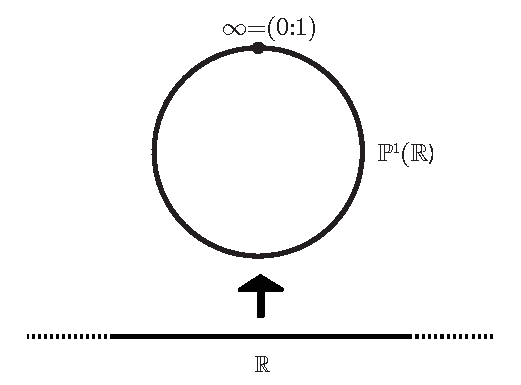
\includegraphics[trim=0cm 0cm 0cm 0cm,clip,scale=0.75]{images/projlinetocirc.pdf}
\end{minipage}
\vspace{-2mm}
\end{example}
\subsection{Chiusura proiettiva di un sottospazio affine}
\begin{define}[Chiusura proiettiva della retta affine.]~{}\\
	Sia $r\subseteq\aff{\kamp^n}$ una retta affine. La \textbf{chiusura proiettiva}\index{chiusura!proiettiva!della retta} di $r$ è il sottospazio proiettivo $\overline{r}\subseteq\proj[n]{\ }$ generato da $r\subseteq U_0\subseteq\proj[n]{\ }$.
\end{define}
\begin{proposition}[Chiusura proiettiva della retta affine.]~{}\\
	$\overline{r}$ è una \textit{retta proiettiva} e si ha:
	\begin{equation}
		\overline{r}=r\cup P_{\infty}
	\end{equation}
Dove $P_{\infty}=\overline{r}\cap H_0$ è detto \textit{punto all'infinito} o \textit{punto improprio} della retta $r$.
\end{proposition}
\begin{demonstration}
	Sia $v\in\kamp^n\setminus\left\{0\right\}$ la direzione di $r$ e $w\in r$ un punto della retta. Allora $r$ ha descrizione parametrica in $\aff{\kamp^n}$:
	\begin{equation*}
		\begin{cases}
			\begin{array}{l}
				X_1=tv_1+w_1\\
				\vdots\\
				X_n=tv_n+w_n\\			
			\end{array}
		\end{cases}\quad t\in\kamp
	\end{equation*}
Consideriamo la retta proiettiva $R\subseteq\proj[n]{\ }$ con descrizione parametrica:
\begin{equation*}
\begin{cases}
		\begin{array}{l}
			x_0=s\\
			x_1=tv_1+sw_1\\
			\vdots\\
			x_n=tv_n+sw_n\\			
		\end{array}
	\end{cases}\quad \left(s\colon t\right)\in\proj[1]{\ }
\end{equation*}
$R$ è la retta proiettiva per i punti:
\begin{equation*}
	t=0\ \colon\ \left(1\colon w_1\colon\ldots\colon w_n\right)\quad s=0\ \colon\ \left(0\colon v_1\colon\ldots\colon v_n\right)=P_\infty
\end{equation*}
Ponendo $s=1$ otteniamo:
\begin{equation*}
	\begin{cases}
		\begin{array}{l}
			x_0=1\\
			x_1=tv_1+w_1\\
			\vdots\\
			x_n=tv_n+w_n\\			
		\end{array}
	\end{cases}\quad t\in\kamp
\end{equation*}
Al variare di $t\in\kamp$, questi sono tutti e soli i punti di $j\left(r\right)\subseteq U_0\subseteq \proj[n]{\ }$. Si ha dunque che $R$ è una retta proiettiva contente $r$:
\begin{equation*}
	\begin{array}{ll}
			R&=r\cup P_{\infty}\\
			P_{\infty}&=R\cap H_0=\left\{\left(0\colon v_1\colon \ldots \colon v_n\right)\right\}
	\end{array}
\end{equation*}
$R$ è necessariamente il più piccolo sottospazio proiettivo contenente $r$, dato che è la retta più un solo punto. Pertanto, $R=\overline{r}$.
\end{demonstration}
\begin{observes}~{}
	\begin{enumerate}
		\item Il punto improprio di $r$ è:
		\begin{equation*}
			P_{\infty}=\left(0\colon v_1\colon \ldots\colon v_n\right)
		\end{equation*}
	E corrisponde esattamente alla \textit{direzione} $v=\left(v_1,\ \ldots,\ v_n\right)$ di $r$.
	Poiché $P_\infty=\left[v\right]$ con $v$ la direzione di $r$, ne segue che l'iperpiano improprio di $\proj[n]{\kamp }$ è:
	 \begin{equation*}
		\begin{array}{ll}
			H_0 & =\proj[n-1]{\kamp}=\proj{\kamp^n}=\left\{\text{rette vettoriali in }\kamp^n\right\}=\\
			&=\left\{\text{direzioni delle rette affini in }\aff{\kamp^n}\right\}
		\end{array}
	\end{equation*}
\item Due rette affini $r_1,\ r_2\subseteq \aff{\kamp^n}$ hanno lo stesso punto improprio se e solo hanno la \textit{stessa direzione}, cioè se sono \textit{parallele}.\\
Se $r_1\neq r_2$ e $r_1$ e $r_2$ sono parallele, allora $r_1\cap r_2=\emptyset$ in $\aff{\kamp^n}$, ma $\overline{r_1}\cap \overline{r_2}={P_{\infty}}$ in $\proj[n]{\ }$. Ciò ci porta a dire che due rette parallele $r_1$ e $r_2$ si incontrano sempre all'\textit{infinito}!
\item Se $n=2$, cioè operando in $\proj[2]{\ }$, due rette distinte $r_1,\ r_2\subseteq \aff{\kamp^2}$ sono o \textit{incidenti} o \textit{parallele}, ma in $\proj[2]{\ }$ si intersecano sempre.
\item Viceversa: sia $l\subseteq \proj[n]{\ }$ una retta proiettiva. Abbiamo due casi:
\begin{itemize}
	\item $l\subseteq H_0,\ l\cap U_0= \emptyset$.
	\item $l\nsubseteq H_0\implies l+H_0=\proj[n]{\ }$.
\end{itemize}
Infatti, si ha che $l+H_0$ è un sottospazio proiettivo che contiene strettamente $H_0$, dato che $l\nsubseteq H_0$, e usando la formula di Grassmann otteniamo:
\begin{equation*}
	\dim\left(l+H_0\right)=\dim l +\dim H_0-\dim \left(l\cap H_0\right)=1+n-1+0=n=\dim \proj[n]{\ }
\end{equation*}
Da cui ricaviamo che $l+H_0 = \proj[n]{\ }$. Sempre dalla formula di Grassmann:
\begin{equation*}
	\dim\left(l\cap H_0\right)=0\implies l\cap H_0=\left\{1 \text{punto}\right\}=\left\{Q\right\}
\end{equation*}
Cioè $l\cap U_0=l\setminus\left\{Q\right\}$. In altre parole, $l$ è una retta affine in $\aff{\kamp^n}$ con un \textit{punto improprio} $Q$ e necessariamente $l$ è la chiusura proiettiva di $l\setminus\left\{Q\right\}$.
\item Sia $n=2$, cioè operiamo in $\proj[2]{\ }$. Una retta $r\subseteq \aff{\kamp^2}$ è descritta da un'equazione lineare:
\begin{equation}
	ax+by+c=0\quad \left(a,\ b\right)\neq\left(0,\ 0\right)
\end{equation}
Con la corrispondenza biunivoca fra le coordinate $\left(x,\ y\right)$ vettoriali e $\left(X_1,\ X_2\right)$ affini. Abbiamo tuttavia anche la corrispondenza con le coordinate omogenee in $\proj[2]{\ }$, rispettivamente $\left(x\colon y\colon z\right)$ e $\left(x_0\colon x_1\colon x_2\right)$.\\
Chiamiamo $\left(x\colon y\colon z\right)$ le coordinate omogenee su $\proj[2]{\ }$ con:
\begin{equation*}
	H_0=\left\{P=\left(x\colon y\colon z\right)\in \proj[2]{\ }\mid z=0\right\}=\left\{P=\left(x\colon y\colon0\right)\in \proj[2]{\ }\right\}
\end{equation*}
Allora la chiusura proiettiva $\overline{r}\subseteq \proj[2]{\ }$ di $r$ ha in $\proj[2]{\ }$ l'equazione lineare omogenea seguente:
\begin{equation}
		ax+by+cz=0
\end{equation}
Infatti, per $z=1$ si ottiene l'equazione di $r$, mentre ponendo $z=0$ (cioè il passaggio per $H_0$) troviamo il punto improprio $P_{\infty}$ di $r$:
\begin{equation*}
		\begin{cases}
		\begin{array}{l}
			z=0\\
			ax+by=0\\	
		\end{array}
	\end{cases}\quad P_{\infty}=\left(-b\colon a\colon 0\right)
\end{equation*}
La direzione della retta $ax+by+c=0$ è data dal punto improprio $P_{\infty}$ e corrisponde al vettore $\left(-b\colon a\colon 0\right)$.
\end{enumerate}
\end{observes}
Generalizziamo il concetto di chiusura proiettiva a un generico sottospazio affine.
\begin{define}[Chiusura proiettiva di un sottospazio.]~{}\\
	Dato $S\subseteq \aff{\kamp^n}$ un sottospazio affine con $S\neq \emptyset$, la \textbf{chiusura proiettiva}\index{chiusura!proiettiva} $\overline{S}\subseteq \proj[n]{\ }$ di $S$ è il sottospazio proiettivo generato da $S$. Esso ha dimensione $\dim \overline{S}=\dim S=m$.
\end{define}
\textbf{Equazioni cartesiane}. Se $S$ come sottospazio affine è dato in forma cartesiana dal sistema lineare $h\times\left(n+1\right)$ seguente:
\begin{gather*}
			Ax+b=0\qquad\left(\begin{array}{c}
		X_1\\
		\vdots\\
		X_n
	\end{array}\right)\in\aff{\kamp^{n}}\\
	\begin{cases}
	\begin{array}{l}
		a_{1,1}X_1+\ldots+a_{1,n}X_n+b_1=0\\
		\vdots\\
		a_{h,1}X_1+\ldots+a_{h,n}X_n+b_h=0\\			
	\end{array}
\end{cases}
\end{gather*}
Allora $\overline{S}$ è descritto dal sistema lineare omogeneo  $h\times\left(n+1\right)$ in $\left(x_0,\ \ldots,\ x_n\right)$ seguente:
\begin{gather*}
	\left(A\mid b\right)x=0\qquad\left(\begin{array}{c}
		x_1\\
		\vdots\\
		x_n\\
		x_0
	\end{array}\right)\in\proj[n]{\ }\\
	\textcolor{red}{\circled{\ast}}\begin{cases}
		\begin{array}{l}
			a_{1,1}x_1+\ldots+a_{1,n}x_n+b_1x_0=0\\
			\vdots\\
			a_{h,1}x_1+\ldots+a_{h,n}x_n+b_hx_0=0\\			
		\end{array}
	\end{cases}
\end{gather*}
\begin{demonstration}
	Studiamo le dimensioni di $S$ e $\overline{S}$ usando i sistemi cartesiani appena definiti:
	\begin{equation*}
		\begin{array}{l}
			\dim S=\dim \kamp^n-\rk\left(A\right)=n-\rk\left(A\right)\\
			\dim \overline{S}=\dim \proj[n]{\ }-\rk\left(A\mid b\right)-1=\left(n+1-\rk\left(A\mid b\right)\right)-1=n-\rk\left(A\mid b\right)\\
		\end{array}
	\end{equation*}
	Per Rouché-Capelli vale $\rk A=\rk \left(A\mid b\right)$ in quanto $S\neq \emptyset$. In questo modo abbiamo dimostrato che $\dim \overline{S}=\dim S$.
\end{demonstration}
I \textit{punti impropri} del sottospazio affine $S$ sono dati da $\overline{S}\cap H_0$, con $\overline{S}$ la chiusura proiettiva di $S$ e $H_0$ l'iperpiano improprio. Dal sistema $\textcolor{red}{\circled{\ast}}$ si ha che $\overline{S}\cap H_0$ è dato da:
\begin{equation*}
	\begin{cases}
		\begin{array}{l}
			x_0=0\\
			a_{1,1}x_1+\ldots+a_{1,n}x_n=0\\
			\vdots\\
			a_{h,1}x_1+\ldots+a_{h,n}x_n=0\\			
		\end{array}
	\end{cases}
\end{equation*}
Esso corrisponde al sistema lineare omogeneo in $\kamp^n$ $Ax=0$ associato al sistema lineare $Ax+b=0$ che definisce $S$. In altre parole, $\overline{S}\cap H_0$ corrisponde al \textit{sottospazio vettoriale direttore} $W\subseteq \kamp^n$ e vale $\overline{S}\cap H_0=\proj{W}$ direzione di $S$. La sua dimensione per definizione di direzione è:
\begin{equation*}
	\dim\left(\overline{S}\cap H_0\right)=\dim S-1=\dim\overline{S}-1
\end{equation*}
\textbf{Equazioni parametriche}. Se $S$ ($\dim S=m$) è data in \textit{forma parametrica} e il sottospazio direttore $W\subseteq \kamp^n$ ha una base $\left\{v_1,\ \ldots,\ v_m\right\}$ (tali che $v_i=\left(V_{i,1},\ \ldots,\ V_{i,n}\right)\in\aff{\kamp^n}$ per un dato sistema di riferimento affine), posto $c\in S$ ricordiamo che l'espressione parametrica di $S$ è:
\begin{gather*}
	X=t_1v_1+\ldots+t_mv_m+c\quad t_1,\ \ldots,\ t_m\in\kamp\\
		\begin{cases}
		\begin{array}{l}
			X_1=t_1V_{1,1}+\ldots+t_mV_{m,1}+C_1\\
			\vdots\\
			X_n=t_1V_{1,n}+\ldots+t_mV_{m,n}+C_n\\			
		\end{array}
	\end{cases}
\end{gather*}
Allora, $\overline{S}$ è il sottospazio generato dagli $m+1$ punti \textit{indipendenti}:
\begin{equation}
	\begin{array}{cc}
		\left(0\colon v_{i,1}\colon\ldots\colon v_{i,n}\right)&i=1,\ \ldots,\ m,\ \text{ e }
		\left(1\colon c_1\colon\ldots\colon c_n\right)
	\end{array}
\end{equation}
Pertanto, $\overline{S}$ ha descrizione parametrica:
\begin{equation*}
			\begin{cases}
		\begin{array}{l}
			x_0=t_0\\
			x_1=t_1v_{1,1}+\ldots+t_mv_{m,1}+t_0c_1\\
			\vdots\\
			x_n=t_1v_{1,n}+\ldots+t_mv_{m,n}+t_0c_n\\			
		\end{array}
	\end{cases}
\end{equation*}
Con $\left(t_0\colon\ldots\colon t_m\right)\in\proj[m]{\ }$.
\subsection{Un esempio di proiettività}
Vediamo un esempio di proiettività di $\proj[1]{\ }$.
\begin{example}
	Si consideri $\proj[1]{\kamp} = \kamp \cup \{\infty\}$ con $\infty=(0\colon 1)$. Sia $f$ una proiettività (dunque biunivoca) definita come:
	\begin{equation*}
		\funztot f {\proj[1]{\ }} {\proj[1]{\ }} {(x_0\colon x_1)} {(ax_0+bx_1\colon cx_0+dx_1)}
	\end{equation*}
	Si ha che $f(0\colon 1)=(b\colon d)$, mentre la sua controimmagine è $f(-b\colon a)=(0\colon 1)$; infatti, siccome le coordinate sono omogenee, basta porre $ax_0+bx_1=0$.\newline
	Sia $t=\frac{x_1}{x_0}$ la coordinata affine su $\kamp$, se $x_0\neq 0$ tutti i punti $(x_0\colon x_1)$ si possono scrivere come $(x_0\colon x_1)=\left( 1\colon \frac{x_1}{x_0} \right)=(1\colon t)$, il che corrisponde al punto $t\in\kamp$ . Vediamo ora come si comporta l'immagine grazie a queste osservazioni se $ax_0+bx_1\neq 0$:
	\begin{gather*}
		f(x_0\colon x_1)=(ax_0+bx_1\colon cx_0+dx_1)= \left(1\colon \frac{cx_0+dx_1}{ax_0+bx_1} \right)  =  \left( 1 \colon  \frac{ x_0 \left( c+ d \frac{x_1}{x_0} \right) }{ x_0 \left( a+ b\frac{ x_1 }{ x_0 } \right)} \right)=\left( 1\colon \frac{dt+c}{bt+a}\right)
	\end{gather*}
	Dunque la proiettività $f$ corrisponde alla trasformazione:
	\begin{equation*}
		\funz F {\kamp\cup \{\infty\}} {\kamp\cup \{\infty\}}\text{ con }F(t)=\begin{cases}
			\frac{dt+c}{bt+a}, & t\in\kamp, \ t\neq -\frac{a}{b}\\
			\infty, & t=-\frac{a}{b}\\
			\frac{d}{b}, & t=\infty
		\end{cases}
	\end{equation*}
	Dove per $t=-\frac{a}{b}$ si ottiene $f(-b\colon a)=(0\colon 1)=\infty$, mentre la prima equazione è detta \textit{trasformazione lineare fratta}, che è definita sulla retta affine tranne dove si annulla il denominatore. \newline
	Notiamo che $F$ diventa un'affinità $\funztot F \kamp \kamp t {\alpha t+\beta}$ se e solo se il denominatore diventa una costante ponendo $b=0$, ovvero se è della forma $F(t)=\alpha$, il che significa che la proiettività fissa il punto all'infinito, ovvero $f(0\colon 1)=(0\colon 1)$, mentre la parte affine viene mandata in se stessa.\newline
	Questo ragionamento si può vedere anche in dimensione superiore.
\end{example}
\subsection{Impratichiamoci! Geometria affine e geometria proiettiva}
\begin{exercise}
	Sia $\kamp=\realset$. Allora, preso $\realset^n$ con la topologia Euclidea e $\proj[n]{\realset}$ con la topologia quoziente, mostrare che $U_0$ è un aperto di $\proj[n]{\realset}$ e che $\funz{j}{\realset^n}{U_0}$ è un omeomorfismo.
\end{exercise}
% aggiungere soluzione
\section{Digressione: spazi proiettivi complessi}
\begin{remember}
	Nel caso di $\realset^n$ si è già visto che lo spazio proiettivo reale è un quoziente del tipo $\displaystyle \proj[n]{\realset}=\frac{\realset^{n+1}\setminus\{0\}}{\sim}$, dunque è dotato in maniera naturale di una topologia.\newline
	Si può anche vedere come \textit{quoziente della sfera} $S^n$ dove si identificano i punti antipodali grazie alla \textit{suriezione} $\surr \pi {S^n} {\proj[n]{\realset}}$; è anche una \textit{varietà topologica compatta} di dimensione $n$. Inoltre $\proj[1]{\realset}\cong S^1$ e abbiamo analizzato il piano proiettivo reale $\proj[2]{\realset}$.
\end{remember}
Anche nel caso complesso per $\proj[n]{\complexset}=\frac{\complexset^{n+1}\setminus\{0\}}{\sim}$ si ha in maniera naturale una topologia quoziente data dalla topologia Euclidea su $\complexset^{n+1}\setminus\{0\} \cong \realset^{n+1}\setminus\{0\}$.\newline
Vogliamo vedere che è una \textit{varietà topologica compatta} di dimensione $\mathbf{2n}$. Infatti, mentre $\proj[n]{\realset}$ è localmente euclideo di dimensione $n$, si ha che $\proj[n]{\complexset}$ localmente si comporta come $\complexset^n\cong\realset^{2n}$, dunque la dimensione topologica è $2n$.
\begin{remember}
	 Ricordiamo la corrispondenza fra numeri complessi, reali e la norma:
	\begin{gather*}
		z_j=x_j+iy_j\implies  z=(z_1,\ \ldots,\ z_{n+1})\in\complexset^{n+1}\longleftrightarrow (x_1,\ y_1,\ \ldots,\ x_{n+1},\ y_{n+1})\in\realset^{2n+2}\\
		\begin{array}{ccc}
			\displaystyle \|z\|^2=\sum_{j=1}^{n+1} \lvert z_j\rvert ^2=\sum_{j=1}^{n+1}\left(\lvert x_j \rvert ^2 +\lvert y_j \rvert ^2\right) & \implies & \displaystyle \ \|\lambda z \| =\sqrt{\sum_{j=1}^{n+1}\lvert \lambda z_j \rvert ^2}=\lvert\lambda\rvert \| z\|,\ \lambda\in\complexset
		\end{array}
	\end{gather*}
\vspace{-3mm}
\end{remember}
\begin{theorema}[${\proj[n]{\complexset}}$ è una varietà topologica di dimensione $2n$.]
\end{theorema}
\begin{demonstration}~{}
	\begin{itemize}
	\item $\proj[n]{\complexset}$ è \textbf{connesso}: è quoziente di $\complexset^{n+1}\setminus\{0\}$, che è connesso.
	\item $\proj[n]{\complexset}$ è \textbf{compatto}: per avere la tesi, si vuole vedere lo spazio come \textit{quoziente di un compatto} o \textit{immagine tramite una funzione continua di un compatto}.
	Ricordiamo la relazione di equivalenza:
		\begin{equation*}
			z\sim w\iff \exists\lambda\in\complexset\setminus\{0\}\colon w=\lambda z
		\end{equation*}
	Vogliamo dimostrare che un sistema completo di rappresentanti del piano proiettivo sono i \textit{punti della sfera complessa} $S^{2n+1}\subseteq \complexset^{n+1}=\realset^{2n+2}$.
	Se $z\in\complexset^{n+1}\setminus\{0\}\implies \|z\|\neq 0$ e pertanto $\underbrace{\frac{1}{\|z\|}\cdot z}_{\in S^{2n+1}}\sim z$. Poiché un sistema completo di rappresentanti è la sfera, si ha $\pi(S^{2n+1})=\proj[n]{\complexset}$ e dunque $\proj[n]{\complexset}$ è compatto.
	\item $\proj[n]{\complexset}$ è di \textbf{Hausdorff}: partiamo con una considerazione che segue dal punto precedente. Nel caso reale i punti sulla sfera sono equivalenti solo se \textit{antipodali}; nel caso complesso la questione è differente. Consideriamo $z,\ w\in S^{2n+1}$; per definizione del piano proiettivo:
		\begin{equation*}
			z\sim w\iff \exists \lambda\in\complexset\setminus\{0\} \colon w=\lambda z
		\end{equation*}
	Siccome $w,\ z\in S^{2n+1}$ hanno norma unitaria $1=\| w\|=\|\lambda z\|= \ \lambda | \|z\|=|\lambda|$. Essendoci \textit{infiniti} numeri di norma $1$ in $\complexset$, allora ci sono \textit{infiniti} numeri nella stessa classe, e quindi i punti $\lambda z\in S^{2n+1}$ sono tutti equivalenti.\\
	Consideriamo ora $\funz{\pi_0=\pi_{\mid S^{2n+1}}}{S^{2n+1}}{\proj[n]{\complexset}}$. Per dimostrare che $\proj[n]{\complexset}$ è di Hausdorff, è sufficiente dimostrare che $\pi_0$ è un'identificazione \textit{chiusa} per il teorema \ref{quozientehausdorff} (pag. \pageref{quozientehausdorff}), ovvero il piano proiettivo si ottiene come quoziente della sfera.\\
	Sia $C\subset S^{2n+1}$ un chiuso. Allora $\pi_0(C)$ è chiuso in $\proj[n]{\complexset}\iff \pi_0^{-1}(\pi_0(C))$ è chiuso in $S^{2n+1}$.
	Per le osservazioni precedenti che:
	\begin{equation*}
		\pi_0\left(z\right)= \pi_0\left(w\right)\iff \exists\lambda\in\complexset\text{ con }\lvert\lambda\rvert=1\colon w=\lambda z
	\end{equation*}
	In effetti la relazione di equivalenza su $S^{2n+1}$ viene da un'azione del gruppo $S^1=\{\lambda\in\complexset \mid |\lambda |=1\}$ rispetto al prodotto con elemento neutro $1$:
	\begin{equation*}
		\funztot F {S^1\times S^{2n+1}} {S^{2n+1}} {(\lambda, z)} {\lambda z}
	\end{equation*}
	\begin{itemize}
		\item $F$ è un'applicazione continua.
		\item $S^1\times S^{2n+1}$ è compatto e \textbf{Hausdorff}.
	\end{itemize}
	$F$ è \textit{chiusa} in quanto funzione continua da un compatto in \textbf{Hausdorff}.\\
	Dato un chiuso $C\subseteq S^{2n+1}$, prendendo la controimmagine dell'immagine agisco sui punti di $C$ con tutti gli elementi di $S^1$, cioè prendo tutte le orbite che intersecano $C$:
	\begin{equation*}
		\pi_0^{-1}(\pi_0(C))=F(\underbrace{S^1\times C}_{\stackrel{\text{chiuso in}}{S^1\times S^{2n+1}}})\subseteq S^{2n+1}\vspace{-2mm}
	\end{equation*}
Segue che $\pi_0^{-1}(\pi_0(C))$ chiuso e $\pi_0(C)$ chiuso in $\proj[n]{\complexset}$, cioè $\pi_0$ è applicazione chiusa e $\pi_0$ identificazione per il teorema \ref{condizione sufficiente identificazione} (Manetti 5.4), pag. \pageref{condizione sufficiente identificazione}.\\
Pertanto $\proj[n]{\complexset}$ è anche quoziente di $S^{2n+1}$.
Siccome $S^{2n+1}$ è un compatto in un \textbf{Hausdorff} e $\pi_0$ è un'identificazione \textit{chiusa} allora $\proj[n]{\complexset}$ è \textbf{Hausdorff} per il teorema citato in precedenza.
\item $\proj[n]{\complexset}$ è \textbf{localmente euclideo di dimensione} $2n$: per dimostrarlo riprendiamo le costruzioni introdotte a pag. \pageref{spaziaffinitoproiettivi}. Consideriamo la famiglia di insiemi:
		\begin{equation*}
			U_j\coloneqq\{z_j\neq 0\}=\proj[n]{\complexset}\setminus H_j\text{, con }H_j\ j\text{-esimo iperpiano coordinato.}
		\end{equation*}
		Per semplicità sia $j=0$.\newline
		Si consideri la proiezione al quoziente $\funz \pi {\complexset^{n+1}\setminus\{0\}} {\proj[n]{\complexset}}$ e la controimmagine $\pi^{-1}(U_0)=\{z\in\complexset^{n+1}\setminus\{0\}\mid z_0\neq 0\}$, aperto in $\complexset^{n+1}\setminus\{0\}$ in quanto abbiamo tolto un iperpiano. Segue che $U_0$ è aperto in $\proj[n]{\complexset}$ e lo stesso vale per tutti gli $U_j$. Si considerano le seguenti mappe biunivoche, una inversa dell'altra:
		\begin{equation*}
			\funztot j {\complexset^n} {U_0} {(z_1,\ \ldots,\ z_n)} {(1\colon z_1\colon \ldots\colon z_n)}\quad \funztot \oldphi {U_0} {\complexset^n} {(z_0\colon\ldots\colon z_n)} {\left( \frac{z_1}{z_0},\ \ldots,\ \frac{z_n}{z_0} \right)}
		\end{equation*}
		Mostriamo che $j$ e $\oldphi$ siano omeomorfismi; siccome sono già biunivoche e una inversa dell'altra basta dimostrare che sono entrambe \textit{continue}.\\
			\begin{minipage}[t]{0.51\textwidth}\vspace{1pt}
				Per mostrare che $j$ è continua consideriamo il diagramma a lato, che rappresenta la fattorizzazione di $j$ in $\complexset^{n+1}\setminus\{0\}$ tramite:
					\begin{equation*}
						\widetilde{j}((z_1,\ \ldots,\ z_n))=(1,\ z_1\ldots,\ z_n)
					\end{equation*}
				E la proiezione $\pi$, che in questo caso opera nel seguente modo:
					\begin{equation*}
					\pi((1,\ z_1\ \ldots,\ z_n))=(1\colon z_1\colon\ldots\colon z_n)
				\end{equation*}
				 Siccome $\widetilde{j}$ e $\pi$ sono continue, allora anche la loro composizione $j$ lo è.
			\end{minipage}\hspace{-15pt}
			\begin{minipage}[t]{0.49\textwidth}\vspace{25pt}
				% https://q.uiver.app/?q=WzAsNCxbMSwwLCJcXGNvbXBsZXhzZXRee24rMX1cXHNldG1pbnVzXFx7MFxcfSJdLFswLDIsIlxcY29tcGxleHNldF5uIl0sWzIsMiwiVV8wIl0sWzEsMl0sWzEsMCwiXFx3aWRldGlsZGV7an0iXSxbMSwyLCJqIiwyXSxbMCwyLCJcXHBpIl1d
				\[\begin{tikzcd}
					& {\complexset^{n+1}\setminus\{0\}} \\
					\\
					{\complexset^n} & {} & {U_0}
					\arrow["{\widetilde{j}}", from=3-1, to=1-2]
					\arrow["{j}"', from=3-1, to=3-3]
					\arrow["{\pi}", from=1-2, to=3-3]
				\end{tikzcd}\]
			\end{minipage}\\
			\begin{minipage}[t]{0.51\textwidth}\vspace{10pt}
				Per la continuità dell'inversa $\oldphi$ si procede con la fattorizzazione tramite una restrizione dell'inversa di $\pi$ a $\pi^{-1}U_0$:
				\begin{equation*}
					\funz {p\coloneqq \pi_{\mid_{\pi^{-1}(U_0)}}} {\pi^{-1}(U_0)} {U_0}
				\end{equation*}
				E tramite $\hat{\oldphi}$:
				\begin{equation*}
					\widehat{\oldphi}(z_0,\ \ldots,\  z_n)=\left( \frac{z_1}{z_0},\ \ldots,\ \frac{z_n}{z_0}\right)
				\end{equation*}
			\end{minipage}\hspace{-15pt}
			\begin{minipage}[t]{0.49\textwidth}\hspace{-15pt}\vspace{25pt}
				% https://q.uiver.app/?q=WzAsNCxbMiwwLCJcXHBpXnstMX0oVV8wKSJdLFszLDAsIlxcc3Vic2V0IFxcY29tcGxleHNldF57fW4rMSJdLFswLDIsIlVfMCJdLFszLDIsIlxcY29tcGxleHNldF5uIl0sWzIsMywiXFxvbGRwaGkiLDJdLFswLDIsInAiLDJdLFswLDMsIlxcaGF0e1xcb2xkcGhpfSJdXQ==
				\[\begin{tikzcd}
					&[-35pt]& {\pi^{-1}(U_0)}\subset \complexset^{n+1} &[-15pt] {} \\
					\\
					{U_0} &&& {\complexset^n}
					\arrow["{\oldphi}"', from=3-1, to=3-4]
					\arrow["{p}"', from=1-3, to=3-1]
					\arrow["{\widehat{\oldphi}}", from=1-3, to=3-4]
				\end{tikzcd}\]
			\end{minipage}\\
		 Entrambe sono \textit{continue}: la prima è la restrizione di una funzione continua e la seconda, essendo ben definita ($U_0=\{z_0\neq 0\}$), risulta banalmente continua: inoltre, quest'ultima lavora solo con vettori e non con classi di equivalenza!\\
		Per dimostrare che $\oldphi$ è continua utilizzeremo le proprietà della topologia quoziente (vedasi \pageref{proprietà identificazione quoziente e mappa continua indotta}), dimostrando che $p$ è un'\textit{identificazione}: è già \textit{continua} e \textit{suriettiva}, dunque basta solo che sia aperta o chiusa per il teorema \ref{condizione sufficiente identificazione}.\\
		Osserviamo che $\funz \pi {\complexset^{n+1}\setminus\{0\}} {\proj[n]{\complexset}}$ è anch'essa un quoziente dato dall'azione del gruppo $G=\complexset\setminus\{0\}$ rispetto al prodotto per la moltiplicazione su $\complexset^{n+1}\setminus\{0\}$. In particolare, è un'azione per omeomorfismi. Infatti, fissato  $\lambda\in\complexset\setminus\{0\}$:
	\begin{equation*}
		\funztot {\theta_\lambda} {\complexset^{n+1}\setminus\{0\}} {\complexset^{n+1}\setminus\{0\}} z {\lambda z}
	\end{equation*}
	È continua: per la proposizione \ref{proiezione azione gruppo aperta} si ha che $\funz \pi {\complexset^{n+1}\setminus\{0\}} {\proj[n]{\complexset}}$ è un'applicazione aperta, pertanto anche $p$ che è una sua restrizione è aperta.
	Dalle considerazioni di cui sopra $p$ è un'identificazione. Ne segue che $U_0$ è un aperto di $\proj[n]{\complexset}$ omeomorfo a $\complexset^n$ e quindi a $\realset^{2n}$.\\
	Allo stesso modo, $\forall j\in\{0,\ \ldots,\ n\},\ U_j$ è un aperto di $\proj[n]{\complexset}$ omeomorfo a $\complexset^n$ tramite la mappa-.
	\begin{equation*}
		\funztot {\oldphi_j} {U_j} {\complexset^n} {(z_0\colon\ldots\colon z_n)} {\left( \frac{z_0}{z_j},\ldots,\frac{z_{j-1}}{z_j}, \frac{z_{j+1}}{z_j},\ldots, \frac{z_n}{z_j} \right)}
	\end{equation*}
	Siccome in \textit{coordinate omogenee} c'è sempre un elemento \textit{non} nullo (si lavora su $\complexset^{n+1}\setminus\{0\}$) allora ogni punto sta in uno degli aperti $U_j$, cioè:
	\begin{equation*}
		\proj[n]{\complexset}=U_0\cup\ldots\cup U_n
	\end{equation*}
	 $\proj[n]{\complexset}$ è \textit{localmente euclideo} di dimensione $2n$, dunque è una \textit{varietà topologica compatta}.
	\end{itemize}
\vspace{-3mm}
\end{demonstration}
\begin{observes}~{}
	\begin{itemize}
		\item Su un campo $\kamp$ qualsiasi si ha sempre la mappa $\oldphi_j$, una corrispondenza biunivoca fra i sottoinsiemi $U_j$ (complementari di un iperpiano coordinato) e $\kamp^n$ (senza aspetto topologico): vale sempre che lo spazio proiettivo è unione di tali $U_j$.\\
		In particolare, nel caso reale, tali $U_j$ sono \textit{aperti} ed il ragionamento è \textit{analogo} a quello fatto poc'anzi nel caso complesso.
		\item Non abbiamo dimostrato che è a base numerabile perché, essendo compatto, segue dal teorema \ref{compattoconnessohausdorfflocalmenteuclideo} (pag. \pageref{compattoconnessohausdorfflocalmenteuclideo}), inoltre si potrebbe dimostrare facilmente ‘‘a mano'' mostrando che gli aperti $U_j$ sono a base numerabile, dunque anche la loro unione finita lo è.
	\end{itemize}
\vspace{-3mm}
\end{observes}

	\subsection{Retta proiettiva complessa}
Cosa succede per la \textit{retta proiettiva complessa}? Essa è una varietà topologica compatta di dimensione $2$ (dunque una \textit{superficie topologica compatta}) che abbiamo già classificato! Scopriamo di che superficie si tratta. Si ha:
\begin{equation}
	\proj[1]{\complexset}=U_0\cup\{(0\colon 1)\}\text{ con } U_0\cong\complexset\cong\realset^2
\end{equation}
In altre parole, la retta proiettiva complessa è un \textit{piano} unito ad un \textit{punto}. Dimostriamo ora che è omeomorfa a $S^2$, detta anche \textbf{sfera di Riemann} \index{sfera!di Riemann}, e analizziamo poi la differenza con il piano proiettivo reale.
\begin{theorema}[${\proj[1]{\complexset}\cong S^2}$.]~{}\\
\end{theorema}
\begin{intuit}
	Per ottenere la sfera si può pensare di \textit{richiudere} il piano $\realset^2$ su se stesso, aggiungendo il punto all'infinito $\{(0\colon 1)\}$.
\end{intuit}
\begin{demonstration}
	Costruiamo l'omeomorfismo con $S^2\subset\realset^3$ attraverso la \textit{proiezione stereografica}. Consideriamo:
		%https://q.uiver.app/?q=WzAsNCxbMCwwLCJTXjJcXHNldG1pbnVzXFx7TlxcfSJdLFsyLDAsIlxccmVhbHNldF4yIl0sWzQsMCwiXFxjb21wbGV4c2V0Il0sWzYsMCwiVV8wIl0sWzAsMSwicF9OIl0sWzEsMiwiayJdLFsyLDMsImoiXSxbMCwzLCJGX3t8X3tTXjJcXHNldG1pbnVzXFx7TlxcfX19IiwyLHsiY3VydmUiOjV9XV0=
		\[\begin{tikzcd}
			{S^2\setminus\{N\}} && {\realset^2} && {\complexset} && {U_0}
			\arrow["{p_N}", from=1-1, to=1-3]
			\arrow["{k}", from=1-3, to=1-5]
			\arrow["{j}", from=1-5, to=1-7]
			\arrow["{F_{\mid_{S^2\setminus\{N\}}}}"', from=1-1, to=1-7, curve={height=30pt}]
		\end{tikzcd}\]
	Con $\funz {p_N} {S^2\setminus\{N\}} {\realset^2}$ la \textit{proiezione stereografica} dal polo nord $N=(0,\ 0,\ 1)$, $\funztot k {\realset^2} \complexset {\left(x,\ y\right)} {x+iy}$ e $\funztot j \complexset {U_0} w {(1\colon w)}$.\\
	Allora definiamo una funzione $F$ su $S^2\setminus\{N\}$:
	\begin{equation*}
		F_{\mid_{S^2\setminus\{N\}}}\coloneqq j\circ k\circ p
	\end{equation*}
	Poniamo $F(N)\coloneqq (0\colon 1)$ in quanto è l'unico punto rimasto da dover ‘‘mappare'', ricordando che $\proj[1]{\complexset}=U_0\cup\{(0\colon 1)\}$. \\
	Siccome $j\ ,\ k,\ p$ sono \textit{tutti} omeomorfismi, allora la loro composizione $F_{\mid_{S^2\setminus\{N\}}}$ è biunivoca e continua su $S^2\setminus\{N\}$.\\
	Perché $F$ sia continua in tutti i suoi punti basta verificarla che lo sia in un intorno (aperto) contenente $N$ perché valga il lemma di incollamento. % è l'unico motivo per cui secondo me ha senso questo: si crea F incollando le due proiezioni stereografiche sulle due sfere bucate.
	Considieriamo la proiezione stereografica dal polo sud $S=(0,\ 0,\ -1)$ scegliamo l'aperto $S^2\setminus\{S\}$, intorno di $N$. Dobbiamo mostrare la continuità di $F_{\mid_{S^2\setminus\{S\}}}$.\\
	Scriviamo le due proiezioni stereografiche, sia da $N$, sia da $S$: fissato un punto $P_0=(x_0,\ y_0,\ z_0)$ sulla sfera, allora consideriamo le semirette uscenti da $N$ e da $S$ che passano per $P_0$ \footnote{Le equazioni sono scritte in \textit{forma parametrica}, pertanto abbiamo evidenziato il punto per cui passano e la direzione.}:
		\begin{gather*}
			\begin{array}{ccc}
				NP_0\colon \begin{cases}
					x=0+tx_0\\
					y=0+ty_0\\
					z=1+t(z_0-1)
				\end{cases}\quad P_0-N & \quad & SP_0\colon \begin{cases}
					x=0+tx_0\\
					y=0+ty_0\\
					z=-1+t(z_0+1)
				\end{cases}\quad P_0-S
			\end{array}
		\end{gather*}
	Per trovare le immagini delle proiezioni stereografiche intersechiamo le due semirette con il piano $xy$, cioè poniamo $z=0$:
		\begin{gather*}
			\begin{array}{ccc}
				N\ \colon  1+t(z_0-1)=0\implies t=\frac{1}{1-z_0} & \quad & S\ \colon -1+t(z_0+1)=0\implies t=\frac{1}{1+z_0}
			\end{array}
		\end{gather*}
	Notiamo che i denominatori non si annullano in entrambi i casi per la definizione delle proiezioni stereografiche sulla sfera meno $N$ ed $S$ rispettivamente.\\
	Ne segue che l'immagine di $\realset^2$ tramite la mappa standard $k$ è:
		\begin{gather*}
			\begin{array}{ccc}
				N\ \colon  \left( \frac{x_0}{1-z_0}, \frac{y_0}{1-z_0} \right) \mapsto w=\frac{x_0}{1-z_0} + i\frac{y_0}{1-z_0} \in\complexset & \quad &  S\ \colon \left( \frac{x_0}{1+z_0}, \frac{y_0}{1+z_0} \right) \mapsto u=\frac{x_0}{1+z_0} + i\frac{y_0}{1+z_0} \in\complexset
			\end{array}
		\end{gather*}
	Si ha che $w=\frac{1}{\overline{u}}$ e, viceversa, $u=\frac{1}{\overline{w}}$; infatti, quando $P_0\in S^2\setminus\{N,S\}$ allora $w,\ u\in\complexset\setminus\{0\}$. Verifichiamolo usando le proprietà dei numeri complessi:
		\begin{gather*}
			\frac{1}{\overline{u}} = \frac{1}{ \frac{x_0}{1+z_0} -i\frac{y_0}{1+z_0} } = \frac{1+z_0}{x_0-iy_0} \stackrel{!}{=} \frac{(x_0+iy_0)(1+z_0)}{x_0^2+y_0^2} \stackrel{!!}{=} \frac{(x_0+iy_0)(1+z_0)}{1-z_0^2}=\frac{x_0+iy_0}{1-z_0}=w
		\end{gather*}
	L'uguaglianza (!) vale perché, in quanto $P_0\neq N,\ S$ allora $x_0+iy_0\neq 0$, mentre quella (!!) segue dal fatto che il punto sta sulla sfera, quindi $x_0^2+y_0^2+z_0^2=1\implies x_0^2+y_0^2=1-z_0^2$.\\
	Abbiamo dunque ottenuto $F_{\mid_{S^2\setminus\{N,S\}}}$ come una composizione di mappe:
		% https://q.uiver.app/?q=WzAsNCxbMCwwLCJTXjJcXHNldG1pbnVzXFx7TixTXFx9Il0sWzIsMCwiXFxyZWFsc2V0XjIiXSxbNCwwLCJcXGNvbXBsZXhzZXQiXSxbNiwwLCJVXzAiXSxbMCwxLCJwX04iXSxbMSwyLCJrIl0sWzIsMywiaiJdLFswLDMsIkZfe3xfe1NeMlxcc2V0bWludXNcXHtOLFNcXH19fSIsMix7ImN1cnZlIjo1fV1d
		\[\begin{tikzcd}
			{S^2\setminus\{N,S\}} && {\realset^2} && {\complexset} && {U_0}
			\arrow["{p_N}", from=1-1, to=1-3]
			\arrow["{k}", from=1-3, to=1-5]
			\arrow["{j}", from=1-5, to=1-7]
			\arrow["{F_{\mid_{S^2\setminus\{N,S\}}}}"', from=1-1, to=1-7, curve={height=30pt}]
		\end{tikzcd}\]
	Dove $j(w)=(1\colon w)=\left( 1\colon \frac{1}{\overline{u}} \right)=(\overline{u}\colon 1)$, lavorando in coordinate omogenee. Inoltre, $F$ si estende in modo continuo su $S^2\setminus\{S\}$:
		% https://q.uiver.app/?q=WzAsOSxbMCwwLCJTXjJcXHNldG1pbnVzXFx7TixTXFx9Il0sWzIsMCwiXFxyZWFsc2V0XjIiXSxbNCwwLCJcXGNvbXBsZXhzZXQiXSxbOCwwLCJVXzAiXSxbMCwxLCJQIl0sWzQsMSwidSJdLFs2LDAsIlxcY29tcGxleHNldCJdLFs2LDEsIlxcb3ZlcmxpbmV7dX0iXSxbOCwxLCIoXFxvdmVybGluZXt1fVxcY29sb24gMSkiXSxbMCwxLCJwX04iXSxbMSwyLCJrIl0sWzIsNiwiYyJdLFs2LDMsImoiXSxbNCw1LCIiLDAseyJzdHlsZSI6eyJ0YWlsIjp7Im5hbWUiOiJtYXBzIHRvIn19fV0sWzUsNywiIiwwLHsic3R5bGUiOnsidGFpbCI6eyJuYW1lIjoibWFwcyB0byJ9fX1dLFs3LDgsIiIsMCx7InN0eWxlIjp7InRhaWwiOnsibmFtZSI6Im1hcHMgdG8ifX19XV0=
		\[\begin{tikzcd}
			{S^2\setminus\{S\}} && {\realset^2} && {\complexset} && {\complexset} && {U_0} \\[-25pt]
			{P} &&&& {u} && {\overline{u}} && {(\overline{u}\colon 1)}
			\arrow["{p_S}", from=1-1, to=1-3]
			\arrow["{k}", from=1-3, to=1-5]
			\arrow["{c}", from=1-5, to=1-7]
			\arrow["{j}", from=1-7, to=1-9]
			\arrow[from=2-1, to=2-5, maps to]
			\arrow[from=2-5, to=2-7, maps to]
			\arrow[from=2-7, to=2-9, maps to]
		\end{tikzcd}\]
	Con $c$ coniugio dei complessi (che è un omeomorfismo). In questo modo $F_{\mid_{S^2\setminus\{S\}}}$ è composizione di omeomorfismi e quindi continua.\\
	Dunque $F$ è continua, chiusa (in quanto funzione da $S^2$ compatto in $\proj[1]{\complexset}$ \textbf{Hausdorff}) e biunivoca, pertanto $F$ è un \textit{omeomorfismo}.
%questo ci dice che f ristretto a s^2-s,n è data da una composizione di mappe: proiezione stereografica da N, identificazione standard con C, mappa j in U_0. Ora al posto di w posso scrivere 1/\overline{u}, che per il quoziente è pari a  grazie alle coordinate omogenee: funziona come un'eliminzione dell'indeterminazione: anche se u=0 non è un problema perché ottengo 0:1. Nella proz ster da S il punto che va nello 0 è il polo nord, e questo ci dice che F si estende in maniera continua su S^n-s mandando P nella proiez ster da S , poi ho la mappa j_1, con tutti omeomorfisi. Dunque F è continua perché composizione di omeomorfismi.
\end{demonstration}
\begin{observe}\textsc{$\proj[1]{\complexset}\neq \proj[2]{\realset}$}.\\
Notiamo che $\proj[1]{\complexset}$ e $\proj[2]{\realset}$ sono entrambe compattificazioni del piano, ma in modo \textit{profondamente diverso}!
\begin{itemize}
	\item $\proj[1]{\complexset}=\complexset\cup\{\infty\}\cong S^2$, è l'unione di un \textbf{piano} con un \textbf{punto all'infinito} ed abbiamo appena dimostrato essere omeomorfo alla \textit{sfera di Riemann} $S^2$.
	\item $\proj[2]{\realset}=\realset^2\cup\proj[1]{\realset}\cong\realset^2\cup S^1$, è il piano unito alla retta impropria $\proj[1]{\realset}$; topologicamente, esso è l'\textbf{interno del disco} omeomorfo a $\realset^2$ unito al bordo $S^1$ con la relazione di equivalenza per i punti antipodali. Per il teorema di classificazione delle superfici compatte (pag. \pageref{classificazionesuperficicompatte}), sappiamo che $S^2\ncong \proj[2]{\realset}$.
\end{itemize}
\vspace{-3mm}
\end{observe}
\section{Birapporto}
Nei nostri precedenti studi di Topologia abbiamo messo in primo piano lo studio delle \textit{proprietà topologiche}, quegli aspetti di uno spazio topologico che si preservano sotto \textit{omeomorfismi}. Anche nella Geometria Proiettiva risulta di fondamentale importanza la ricerca di \textbf{invarianti} rispetto alle proiettività.\\
Nella geometria Euclidea del piano diverse trasformazioni mantengono relazioni metriche come distanze, angoli e rapporti di distanze, ma passando alla \textit{retta proiettiva} la maggior parte di queste vengono \textit{distorte}. Tuttavia, già nella matematica del tardo periodo greco si trovò che un \textit{rapporto di rapporto di distanze} sul piano si preservava tramite certe trasformazioni.\\
Questo concetto, approfondito e generalizzato (separandolo completamente dalla \textit{distanza Euclidea}) nell'ottica della Geometria proiettiva nel \textit{secolo XIX}, diventò il \textbf{birapporto}, risultando uno degli invarianti proiettivi più usati.
\begin{define}[Birapporto.]~{}\\
	Sia $\proj[1]{V}$ una retta proiettiva, ovvero $\dim V=2$.\\
	Siano $P_1,\ P_2,\ P_3,\ P_4\in\proj[1]{V}$ dei punti con $P_1,\ P_2,\ P_3$ distinti. Il \textbf{birapporto}\index{birapporto} dei punti $P_1,\ P_2,\ P_3,\ P_4$ (ordinati) è:
		\begin{equation}
			\beta(P_1,\ P_2, P_3, P_4)=\frac{y_1}{y_0}\in\kamp\cup\{\infty\}\text{ con }\beta=\infty\text{ se }y_0=0
		\end{equation}
	Dove $(y_0\colon y_1)$ sono le coordinate di $P_4$ nel riferimento proiettivo in cui $P_1$ e $P_2$ sono i punti fondamentali e $P_3$ il punto unità, cioè $P_1=(1\colon 0), P_2=(0\colon 1), P_3=(1\colon 1)$.
\end{define}
\begin{observes}~{}
	\begin{enumerate}
		\item $y_0,y_1\in\kamp\implies\beta\in\kamp\cup\{\infty\}$
		\item $\beta$ è ben definito perché $P_1,\ P_2,\ P_3$ sono distinti e quindi sono in posizione generale \footnote{In una retta proiettiva essere distinti equivale ad essere in posizione generale.}, ovvero determinano in maniera univoca il riferimento proiettivo per il teorema \ref{puntiposizionegeneraleesistenzabase}, pag. \pageref{puntiposizionegeneraleesistenzabase}.
		\item Per ipotesi i primi tre punti sono distinti, mentre non si fanno ipotesi sul quarto punto; vediamo cosa succede in alcuni casi speciali:\label{birapporto2punti}
			\begin{equation*}
				\begin{array}{lllllll}
					P_4=P_1 &\iff& (y_0\colon y_1)=(1\colon 0)&&&\iff& \beta=0\\
					P_4=P_2 &\iff& (y_0\colon y_1)=(0\colon 1)&&& \iff&\beta=\infty\\
					P_4=P_3 &\iff& (y_0\colon y_1)=(1\colon 1)&\iff& y_0=y_1 &\iff&\beta=1
				\end{array}
			\end{equation*}
		Dunque $\beta\in\{0,1,\infty\}$ esattamente quando $P_4$ coincide con uno dei primi 3 punti. Quindi, se $P_1,\ P_2,\ P_3,\ P_4$ sono distinti. allora $\beta\in\kamp\setminus\{0,1\}$. \\
		Viceversa se $a\in\kamp\setminus\{0,1\}$ e $P_4=(1\colon a)$ allora $\beta=a$, dunque $\beta$ assume tutti i valori possibili in $\kamp$.
	\end{enumerate}
\vspace{-3mm}	
\end{observes}
Vogliamo ora scoprire come si calcola il birapporto non solo nel sistema di riferimento della definizione, ma in uno qualunque.
\begin{theorema}[Birapporto di quattro punti.]~{}\\
	Siano $P_1,\ P_2,\ P_3,\ P_4\in\proj[1]{V}$ dei punti nella retta proiettiva con $P_1,\ P_2,\ P_3$ distinti. Supponiamo che $P_i=(\lambda_1\colon \mu_i), i=1,\ \ldots,\ 4$. Allora:
		\begin{equation}
			\beta(P_1,\ P_2,\ P_3,\ P_4)=\frac{ \left| \begin{array}{cc}
					\lambda_1 & \lambda_4 \\
					\mu_1 & \mu_4
				\end{array} \right| \cdot \left| \begin{array}{cc}
				\lambda_2 & \lambda_3 \\
				\mu_2 & \mu_3
			\end{array} \right| } { \left| \begin{array}{cc}
			\lambda_1 & \lambda_3 \\
			\mu_1 & \mu_3
		\end{array} \right| \cdot \left| \begin{array}{cc}
		\lambda_2 & \lambda_4 \\
		\mu_2 & \mu_4
	\end{array} \right| }
		\end{equation}
	\vspace{-3mm}
\end{theorema}
\begin{demonstration}
	Poiché $P_1\neq P_2$, si ha che $(\lambda_1,\mu_1),(\lambda_2,\mu_2)$ sono una base di $\kamp^2$. Siano ora:
	\begin{equation*}
	\textcolor{blueill}{\circled{\ast}}\quad	a,\ b\in\kamp \colon (\lambda_3,\mu_3)=a(\lambda_1,\mu_1)+b(\lambda_2,\mu_2)=(a\lambda_1,a\mu_1)+(b\lambda_2,b\mu_2)
	\end{equation*}
	In sostanza, facciamo una \textit{combinazione lineare} e portiamo dentro gli scalari. Per costruzione con questi vettori ottengo la base che dà il riferimento proiettivo con $P_1,\ P_2$ punti fondamentali e $P_3$ punto unità (riscalando in modo tale che sia la somma degli altri due vettori). Per ottenere $P_4$, scrivo il corrispettivo vettore come una combinazione lineare dei vettori della base:
	\begin{equation*}
		\textcolor{redill}{\circled{\ast}}\quad	\exists c,d\in\kamp \colon (\lambda_4,\mu_4)=c(a\lambda_1,a\mu_1)+d(b\lambda_2,b\mu_2)
	\end{equation*}
	Segue che $P_4$ ha coordinate $(c\colon d)$ nel nuovo riferimento proiettivo e quindi $\beta=\frac{d}{c}$.\\
	Per non appesantire la scrittura useremo come la seguente notazione per i determinanti:
	\begin{equation*}
		\delta_{ij}=\left| \begin{array}{cc}
			\lambda_i & \lambda_j \\
			\mu_i & \mu_j
		\end{array} \right|
	\end{equation*}
	Notiamo che la prima combinazione lineare $\textcolor{blueill}{\circled{\ast}}$ dà il seguente sistema lineare di 2 equazioni in 2 incognite $a,\ b$:
	\begin{equation*}
		\begin{cases}
			\lambda_1 a+\lambda_2 b=\lambda_3\\
			\mu_1 a+\mu_2 b=\mu_3
		\end{cases}
	\end{equation*}
	Risolvendo il sistema con il metodo di Cramer\footnote{Nelle ‘‘Note aggiuntive'', a pag. \pageref{Cramerrimembriancor}, si possono trovare alcuni brevi cenni al metodo di Cramer.} si ottiene:
	\begin{equation*}
		a=\frac{\left| \begin{array}{cc}
				\lambda_3 & \lambda_2 \\
				\mu_3 & \mu_2
			\end{array} \right| }{ \left| \begin{array}{cc}
				\lambda_1 & \lambda_2 \\
				\mu_1 & \mu_2
			\end{array} \right| } = \frac{\delta_{32}}{\delta_{12}}
		\qquad
		b=\frac{\left| \begin{array}{cc}
				\lambda_1 & \lambda_3 \\
				\mu_1 & \mu_3
			\end{array} \right| }{ \left| \begin{array}{cc}
				\lambda_1 & \lambda_2 \\
				\mu_1 & \mu_2
			\end{array} \right| } = \frac{\delta_{13}}{\delta_{12}}
	\end{equation*}
	La seconda combinazione lineare $\textcolor{redill}{\circled{\ast}}$ invece dà un sistema lineare in $c,\ d$, dove sostituisco i valori di $a,\ b$ trovati :
	\begin{equation*}
	\begin{cases}
		(a\lambda_1)c + (b\lambda_2)d=\lambda_4\\
		(a\mu_1)c + (b\mu_2)d=\mu_4
	\end{cases}	\Rightarrow \begin{cases}
		\frac{\delta_{32}}{\delta_{12}}\lambda_1 c + \frac{\delta_{13}}{\delta_{12}}\lambda_2 d = \lambda_4\\
		\frac{\delta_{32}}{\delta_{12}}\mu_1 c + \frac{\delta_{13}}{\delta_{12}}\mu_2 d = \mu_4
	\end{cases}
	\Rightarrow \begin{cases}
		(\delta_{32}\lambda_2)c + (\delta_{13}\lambda_2)d=\delta_{12}\lambda_4\\
		(\delta_{32}\mu_2)c + (\delta_{13}\mu_2)d=\delta_{12}\mu_4	
	\end{cases}
	\end{equation*}
	Applicando ancora Cramer, poiché il determinante è lineare in ogni colonna, possiamo estrarre i $\delta_{ij}$ dalle colonne e riscriverli \textit{riordinando gli indici}: scambiamo l'ordine delle colonne cambiamo il segno, ma facendolo sia al numeratore, sia al denominatore, i segni si semplificano e lo stesso vale per $d$:
		\begin{equation*}
			\begin{array}{l}
			c=\frac{ \left| \begin{array}{cc}
					\delta_{12}\lambda_4 & \delta_{13}\lambda_2 \\
					\delta_{12}\mu_4 & \delta_{13}\mu_2
			\end{array} \right| }{ \left| \begin{array}{cc}
				\delta_{32}\lambda_1 & \delta_{13}\lambda_2 \\
				\delta_{32}\mu_1 & \delta_{13}\mu_2
			\end{array} \right|  } = \frac{ \cancel{ \delta_{12} } \cancel{\delta_{13}} \delta_{42} }{ \delta_{32} \cancel{\delta_{13}}\cancel{\delta_{12}} } = \frac{-\delta_{24} }{-\delta_{23} }=\frac{\delta_{24}}{\delta_{23}} \\
			\\
			d=\frac{ \left| \begin{array}{cc}
				\delta_{32}\lambda_1 & \delta_{12}\lambda_4 \\
				\delta_{32}\mu_1 & \delta_{12}\mu_4
			\end{array} \right| }{ \delta_{32} \delta_{13} \delta_{12} } = \frac{ \cancel{\delta_{32}} \cancel{\delta_{12}} \delta_{14} }{\cancel{\delta_{32}} \delta_{13} \cancel{\delta_{12}} } = \frac{\delta_{14}}{\delta_{13}}\\
			\implies \beta=\frac{d}{c}=\frac{\delta_{14}}{\delta_{13}}\cdot \frac{\delta_{23}}{\delta_{24}}
		\end{array}
		\end{equation*}					
\end{demonstration}
\begin{observe}
	Il birapporto può anche essere definito tramite questa formula, che è \textit{ben definita}: supponendo di moltiplicare i punti per uno scalare, la stessa costante appare al numeratore e al denominatore, dunque si semplifica, pertanto il birapporto così definito \textit{non dipende} dalla scelta delle coordinate omogenee. Inoltre, al denominatore il primo determinante è sempre diverso da $0$ perché \textit{i punti sono distinti}, mentre il secondo determinante al denominatore è \textit{nullo} se e solo $P_2=P_4$, ottenendo la definizione originale.	
\end{observe}

\begin{tips}
Se tutti e 4 i punti sono diversi da $(0\colon 1)$, ovvero se $\forall i,\ \lambda_i\neq 0\ P_i=(1\colon z_i),\ i=1,\ \ldots,\ 4$ allora:
\begin{equation}
	\beta(P_1,\ P_2,\ P_3,\ P_4)=\frac{ (z_4-z_1)(z_3-z_2) }{ (z_4-z_2)(z_3-z_1) }
\end{equation}
Infatti, $P_i=(\lambda_i\colon\mu_i)=(1\colon z_i)$, cioè  $z_i=\frac{\mu_i}{\lambda_i}$; per la linearità delle colonne si ottiene:
	\begin{gather*}
		\left| \begin{array}{cc}
			\lambda_1 & \lambda_4 \\
			\mu_1 & \mu_4
		\end{array} \right| = \lambda_1\lambda_4 \left| \begin{array}{cc}
		1 & 1 \\
		\frac{\mu_1}{\lambda_1} & \frac{\mu_4}{\lambda_4}
		\end{array} \right|= \lambda_1\lambda_4 \left| \begin{array}{cc}
			1 & 1 \\
			z_1 & z_4
		\end{array} \right| = \lambda_1\lambda_2(z_4-z_1)
	\end{gather*}
Procedendo allo stesso modo con gli altri determinanti e applicando la definizione equivalente di \textit{birapporto}, si ottiene il risultato di sopra in quando i $\lambda$ si semplificano.
\end{tips}
%LEZ 32
\subsection{Birapporto e trasformazioni proiettive}
\begin{remember}
	Date due rette proiettive $\proj[1]{V}$ e $\proj[1]{V'}$ ($\dim \proj[1]{V}=1=\dim \proj[1]{V'}$), e $P_1,\ P_2,\ P_3 \in \proj[1]{V}$ distinti e $Q_1,\ Q_2,\ Q_3 \in \proj[1]{V'}$ distinti, esiste sempre ed è unica una trasformazione proiettiva $\funz f {\proj[1]{V}} {\proj[1]{V'}}$ tale che $f(P_i)=Q_i, \ i=1,2,3$ grazie al il teorema \ref{puntigeneralitrasformazioni}, pag. \pageref{puntigeneralitrasformazioni}.
\end{remember}
Ci interessa ora provare un risultato più generale: l'esistenza di una proiettività con $4$ punti \textit{non tutti in posizione generale}.
\begin{theorema}[Esistenza di una proiettività tra rette proiettive con 4 punti {(di cui 3 distinti)}.]~{}\\
	Siano $\proj[1]{V}$ e $\proj[1]{V'}$ due rette proiettive, con:
	\begin{itemize}
		\item $P_1,\ P_2,\ P_3,\ P_4\in\proj[1]{V}$ (di cui i primi 3 distinti).
		\item $Q_1,\ Q_2,\ Q_3,\ Q_4\in\proj[1]{V'}$ (di cui i primi 3 distinti).
	\end{itemize}
	Allora $\exists$ trasformazione proiettiva $\funz f {\proj[1]{V}} {\proj[1]{V'}}$ tale che:
	\begin{equation}
		f(P_i)=Q_i,\ \forall i=1,\ \ldots,\ 4  \iff \beta(P_1,\ P_2,\ P_3,\ P_4)=\beta(Q_1,\ Q_2,\ Q_3,\ Q_4)
	\end{equation}
\vspace{-3mm}
\end{theorema}
\begin{observe}
	Consideriamo i primi 3 punti e scegliamone dei rappresentanti per cui:
	\begin{equation*}
		v_1,\ v_2,\ v_3\in V \colon P_i=[v_i],\ i=1,\ 2,\ 3\text{ e }v_3=v_1+v_2
	\end{equation*}
	In altri termini, $\{v_1,v_2\}$ è base di $V$ che dà il riferimento proiettivo di $\proj[1]{V}$ in cui $P_1=(1\colon 0),\ P_2=(0\colon 1),\ P_3=(1\colon 1)$. Sia $P_4=[v_4]$ con $v_4=av_1+bv_2$. Allora $P_4=(a\colon b)$ e $\beta(P_i)=\frac{b}{a}$.\\
	Allo stesso modo per l'altra quaterna, siano:
	\begin{equation*}
		v'_1,\ v'_2,\ v'_3\in V' \colon Q_i=[v'_i],\ i=1,\ 2,\ 3\text{ con }v'_3=v'_1+v'_2
	\end{equation*}
	Siccome $P_1,\ P_2,\ P_3$ e $Q_1,\ Q_2,\ Q_3$ sono in posizione generale, allora \textit{esiste ed è unica} una trasformazione proiettiva $\funz f {\proj[1]{V}} {\proj[1]{V'}}$ tale che $f(P_i)=Q_i$.\\
	Inoltre, $f=\widetilde{\phi}$ con $\funz \phi V {V'}$ applicazione lineare tale che $\phi(v_1)=v'_1,\ \phi(v_2)=v'_2$, cioè porta una base di $V$ in una base di $V'$; segue che $\phi(v_4)=\phi(av_1+bv_2)=av'_1+bv'_2$ e pertanto
	$ f(P_4)=[\phi(v_4)]=(a\colon b)$ nel riferimento in $\proj[1]{V'}$.
\end{observe}
\begin{demonstration}~{}\\
	$\impliesdx$Siccome $f$ è unica e $f(P_4)=Q_4 \implies Q_4=(a\colon b)$ nel riferimento in cui $Q_1=(1\colon 0),\ Q_2=(0\colon 1),\ Q_3=(1\colon 1) \implies \beta(Q_1,\ Q_2,\ Q_3,\ Q_4)=\frac{b}{a}=\beta(P_1,\ P_2,\ P_3,\ P_4)$.\\
	$\impliessx$Se $\beta(Q_1,\ Q_2,\ Q_3,\ Q_4)=\frac{b}{a}$, allora distinguiamo i casi in cui il birapporto è in $\kamp$ o \textit{infinito}:
	\begin{itemize}
		\item $\begin{array}{lllll}
			\frac{b}{a}\in\kamp & \implies & Q_4=\left(1\colon \frac{b}{a} \right)=(a\colon b)=f(P_4) &  &
		\end{array}$
		\item $\begin{array}{lllll}
			\frac{b}{a}=\infty & \implies & a=0 & \implies & Q_4=(0\colon 1)=f(P_4)\end{array}$
	\end{itemize}
\vspace{-3mm}
\end{demonstration}
\begin{corollary}[Birapporto è invariante proiettivo.]~{}\\
	Siano $\proj[1]{\kamp}$ e siano dati i punti $P_1,\ P_2,\ P_3,\ P_4\in\proj[1]{\kamp}$ di cui i primi 3 distinti, e altri quattro punti $Q_1,\ Q_2,\ Q_3,\ Q_4\in\proj[1]{\kamp}$ di cui i primi 3 distinti. Allora $\exists$ proiettività $\funz f {\proj[1]{\kamp}} {\proj[1]{\kamp}}$ tale che:
	\begin{equation}
		f(P_i)=Q_i,\ \forall i=1,\ \ldots,\ 4  \iff \beta(P_i)=\beta(Q_i)
	\end{equation}
Cioè se il birapporto delle quaterne è \textbf{invariante per proiettività}.
\end{corollary}

\begin{observe}
	Sia $\mathcal{S}=\{\text{quaterne ordinate di punti distinti in } \proj[1]{\kamp}\}$. Prese due quaterne $\{P_1,\ P_2,\ P_3,\ P_4\}, \{Q_1,\ Q_2,\ Q_3,\ Q_4\} \in\mathcal{S}$, esse sono \textit{proiettivamente equivalenti} se $\exists f$ proiettività tale che $f(P_i)=Q_i
	,\ \forall i=1,\ 2,\ 3,\ 4$ e quindi, in base al teorema precedente, è vero se le due quaterne hanno lo stesso birapporto.\\
	Notiamo	che quella appena data è una \textbf{relazione di equivalenza} %(verifica per esercizio)
	, tale per cui le classi di equivalenza \textit{proiettiva} di $4$ punti \textit{distinti e ordinati} in $\proj[1]{\kamp}$ sono in corrispondenza biunivoca con il campo $\kamp$ escluso $0$ e $1$ visto che sono 4 punti distinti\footnote{Si veda l'analisi dei casi del birapporto con 2 punti uguali a pag. \pageref{birapporto2punti}}, val a dire:
		\begin{equation*}
			\frac{\mathcal{S}}{\sim} \substack{\longleftrightarrow}{\beta}\in\kamp\setminus\{0,1\}
		\end{equation*}
	Si ha dunque che ad ogni quaterna di punti distinti associamo il suo \textit{birapporto} (l'applicazione è \textit{suriettiva}) e per ogni elemento nel campo troviamo una \textit{quaterna di punti distinti} con tale birapporto (quozientando, l'applicazione è iniettiva)
\end{observe}
%"il birapporto misura l'equivalenza proiettiva su punti di una retta proiettiva"

\begin{attention}
	In dimensione maggiore generalmente il birapporto \textit{non è definito}, a meno che i $4$ punti non siano \textit{allineati} su una retta proiettiva $r$.
\end{attention}


\begin{example}~{}\\
	Nel piano proiettivo $\proj[2]{\kamp}$ consideriamo due quaterne di punti distinti $\{P_1,\ P_2,\ P_3,\ P_4\}$ e $\{Q_1,\ Q_2,\ Q_3,\ Q_4\}$. Scelta una quaterna, le disposizioni possibili sono le seguenti:
	\begin{itemize}
		\item In \textbf{posizione generale}, cioè a 3 a 3 non allineati.
\begin{center}
			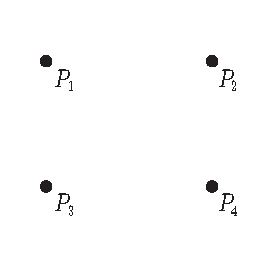
\includegraphics[trim=0cm 0cm 0cm 0cm,clip,scale=0.50]{images/fourpoints1.pdf}
\end{center}
		\item 3 punti allineati su una retta.
\begin{center}
			
\includegraphics[trim=0cm 0cm 0cm 0cm,clip,scale=0.50]{images/fourpoints2.pdf}
\end{center}
		\item 4 punti allineati su una retta.
\begin{center}
			
\includegraphics[trim=0cm 0cm 0cm 0cm,clip,scale=0.50]{images/fourpoints3.pdf}
\end{center}
	\end{itemize}
	Se i punti $P_i$ sono proiettivamente equivalenti ai punti $Q_i$, allora tali posizioni \textit{devono essere mantenute}: le proiettività mandano \textit{rette in rette}, \textit{posizioni generali in posizioni generali}. Per contronominale, se si verificano casi diversi per le due quaterne possiamo affermare che \textit{non} sono proiettivamente equivalenti.
	\begin{enumerate}
		\item Sia $P_i$, sia $Q_i$ sono in \textit{posizione generale}. Siccome abbiamo 4 punti e $4=\dim\proj[2]{\kamp}+2$, allora $\exists !$ proiettività $f$ di $\proj[2]{\kamp}$ tale che $f(P_1)=Q_i, i=1,\ \ldots,\ 4$.
		\item $P_1,\ P_2,\ P_3$ \textbf{allineati ma non} $P_4$, \textbf{e lo stesso per i} $Q_i$; in altre parole, $P_1,\ P_2,\ P_3\in r$ retta proiettiva e $Q_1,\ Q_2,\ Q_3\in s$ retta proiettiva.
		\begin{center}
		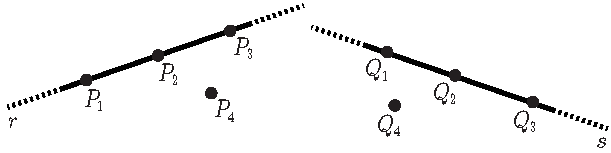
\includegraphics[trim=0cm 0cm 0cm 0cm,clip,scale=0.50]{images/fourpointseq1.pdf}
		\end{center}
		Vogliamo dimostrare che anche in questo caso le quaterne sono proiettivamente equivalenti, estendendo la proiettività fra i tre punti  al quarto.\\
		Scegliamo dei rappresentanti $P_i=[v_i],\ i=1,\ 2,\ 3,\ 4, v_i\in\kamp^3$ tale che $v_3=v_1+v_2$, lecito in quando i punti sono allineati. Si ha che $\{v_1,\ v_2,\ v_4\}$ è una base di $\kamp^3$: $P_4\notin r$ significa che $v_4$ non è linearmente dipendente da $v_1,\ v_2$. Allo stesso modo sia $Q_i=[w_i],\ i=1,\ 2,\ 3,\ 4, w_i\in\kamp^3$ tale che $w_3=w_1+w_2$ con $\{w_1,\ w_2,\ w_4\}$ base di $\kamp^3$. Definiamo $\funz \phi {\kamp^3} {\kamp^3}$ lineare tale che:
		\begin{equation*}
			\phi(v_1)=w_1,\ \phi(v_2)=w_2,\ \phi(v_4)=w_4
		\end{equation*}
		Allora $\phi(v_3)=\phi(v_1+v_2)=w_1+w_2=w_3$ e dunque $\! \funz {f=\widetilde{\phi}} {\proj[2]{\kamp}} {\proj[2]{\kamp}}$ è una proiettività che manda $P_i$ in $Q_i,\ \forall i=1,\ 2,\ 3,\ 4$.
		\item \textbf{Tutti i punti sono allineati}.
		\begin{center}
		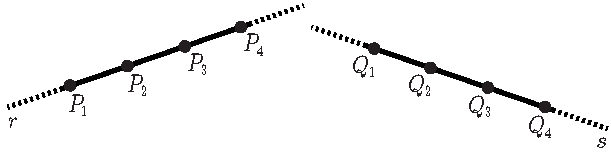
\includegraphics[trim=0cm 0cm 0cm 0cm,clip,scale=0.50]{images/fourpointseq2.pdf}
		\end{center}
		Essendo allineati, allora è definito il loro birapporto. Se le due quaterne sono proiettivamente equivalenti, sia $\funz f {\proj[2]{\kamp}} {\proj[2]{\kamp}}$ la proiettività: essa porta una quaterna nell'altra e necessariamente una retta nell'altra, ovvero $f(r)=s$; in altre parole, la restrizione alle due rette $\funz {f_{\mid_r}} r s$ porta $P_i$ in $Q_i,\ \forall i \implies \beta(P_i)=\beta(Q_i)$.\\
		Viceversa, se $\beta(P_i)=\beta(Q_i)$ allora $\exists \funz g r s$ trasformazione proiettiva che manda $P_i$ in $Q_i,\ \forall i=1,\ 2,\ 3,\ 4$.\\
		Si ha che $g$ si estende in maniera non unica ad una proiettività di $\proj[2]{\kamp}$. Infatti, dati:
		\begin{itemize}
			\item $r=\proj{U},\ U\subset \kamp^3$.
			\item $s=\proj{W},\ W\subset\kamp^3$.
		\end{itemize}
		Con $U$ e $W$ piani vettoriali, si ha che $g=\widetilde{\psi}$ con $\funz \psi U W$ è un isomorfismo lineare. Vogliamo estenderla ad un \textit{automorfismo lineare} $\funz \phi {\kamp^3} {\kamp^3}$ scegliendo basi con due vettori nel piano ed uno esterno, ovvero $u_1,\ u_2\in U$ base di $U$ e $u_3\notin U$. Dunque $\{\psi(u_1),\psi(u_2)\}$ è una base di $W$ e $w_3\notin W \implies \{u_1,u_2,u_3\}$ base di $\kamp^3$ e $\{\psi(u_1),\psi(u_2),w_3\}$ un'altra base. Ponendo $\funz \phi {\kamp^3} {\kamp^3}$ tale che:
		\begin{itemize}
			\item $\phi(u_1)\coloneqq \psi(u_1)$.
			\item $\phi(u_2)\coloneqq \psi(u_2)$.
			\item $\phi(u_3)\coloneqq w_3$
		\end{itemize}
		Si ha $f=\widetilde{\phi}$. Dunque, i punti sono \textit{proiettivamente equivalenti} se e solo se hanno lo \textit{stesso birapporto}.
	\end{enumerate}
\vspace{-3mm}
\end{example}
\subsection{Eserciziamoci! Birapporto}
\begin{exercise}
	Verificare che se $P_1,\ P_2,\ P_3,\ P_4$ sono tutti diversi da $(1\colon 0)$, cioè $P_i=(w_i\colon 1),\ \forall i=1,\ \ldots,\ 4$ allora vale:
	\begin{equation}
		\beta=\frac{ (w_2-w_1)(w_3-w_2) }{ (w_4-w_2)(w_3-w_1) }
	\end{equation}
\vspace{-3mm}
\end{exercise}
	% aggiungere soluzione
		\section{Piano proiettivo duale}
Una \textbf{retta} in $\proj[2]{\kamp}$ ha equazione:
\begin{equation}
	r\ \colon a_0x_0+a_1x_1+a_2x_2=0
\end{equation}
Essa è un'\textbf{equazione lineare omogenea} in coordinate omogenee, dunque è determinata dai coefficienti $a_0,\ a_1,\ a_2$ dell'equazione con la proprietà che devono essere \textit{non tutti nulli}; inoltre, fissati i coefficienti, l'equazione è determinata \textit{a meno di costante moltiplicativa non nulla}. Dunque si può associare a $r$ un \textbf{punto} del piano proiettivo dato dai coefficienti delle coordinate omogenee:
\begin{equation}
	(a_0\colon a_1\colon a_2)\in\proj[2]{\kamp}
\end{equation}
Si ha una \textit{corrispondenza biunivoca} fra le rette in $\proj[2]{\kamp}$ e lo spazio proiettivo in sè:
	% https://q.uiver.app/?q=WzAsNCxbMCwwLCJcXHtcXHRleHR7cmV0dGUgaW4gfSBcXHByb2pbMl17XFxrYW1wfVxcfSJdLFszLDAsIlxccHJvalsyXXtcXGthbXB9Il0sWzAsMSwiclxcY29sb24gYV8weF8wK2FfMXhfMSthXzJ4XzI9MCJdLFszLDEsIihhXzBcXGNvbG9uIGFfMVxcY29sb24gYV8yKSJdLFswLDEsIiIsMCx7InN0eWxlIjp7InRhaWwiOnsibmFtZSI6ImFycm93aGVhZCJ9fX1dLFsyLDMsIiIsMCx7InN0eWxlIjp7InRhaWwiOnsibmFtZSI6ImFycm93aGVhZCJ9fX1dXQ==
	\[\begin{tikzcd}
		{\{\text{rette in } \proj[2]{\kamp}\}} &&& {\proj[2]{\kamp}} \\[-25pt]
		{r\colon a_0x_0+a_1x_1+a_2x_2=0} &&& {(a_0\colon a_1\colon a_2)}
		\arrow[from=1-1, to=1-4, tail reversed]
		\arrow[from=2-1, to=2-4, tail reversed]
	\end{tikzcd}\]
% Notiamo che ciò funziona bene con $\proj[2]{\kamp}$, infatti le coordinate omogenee si comportano proprio come i coefficienti dell'equazione.
\begin{example}
In $\proj[2]{\realset}$:
		\begin{equation*}
			l_i\colon x_0+x_1+2x_2=0 \longleftrightarrow (1\colon 1\colon 2)\in\proj[2]{\realset}
		\end{equation*}
	\vspace{-6mm}
\end{example}
\begin{define}[Piano proiettivo duale.]~{}\\
	Inteso $\proj[2]{\kamp}$ come lo spazio che \textit{parametrizza le rette} in $\proj[2]{\kamp}$, lo chiamiamo \textbf{piano proiettivo duale} \index{piano!proiettivo!duale} e lo denotiamo con $\proj[2]{\kamp}^{\ast}$.
\end{define}
In prima istanza, questo significa semplicemente che si interpreta un punto del \textit{piano duale} come un punto \textit{associato} ad una \textit{retta} di $\proj[2]{\kamp}$.
%collgamento co lo spazio vettoriale duale forma lineare, prima costruzione come corrispondenza
\subsection{Fascio di rette}
\begin{define}[Fascio di rette.]~{}\\
	Un \textbf{fascio di rette}\index{fascio!di rette} $\mathcal{F}$ in $\proj[2]{\kamp}$ è l'insieme delle rette di equazione:
		\begin{equation}
			\mathcal{F}\colon \lambda l_1+\mu l_2=0, \ (\lambda\colon\mu)\in\proj[1]{\kamp}
		\end{equation}
	Dove $l_1,\ l_2$ sono due rette fissate e distinte.
\end{define}
\begin{observe}
	Possiamo pensare al fascio di rette come una \textbf{collezione di rette}, le cui equazioni si ottengono come \textit{combinazione lineare} delle due rette del fascio con $\lambda,\ \mu$ come \textbf{parametri}.
\end{observe}
\begin{example}
	Consideriamo le rette $l_1\colon x_0+x_1+2x_2=0$ e $l_2\colon 3x_0-2x_1+4x_2=0$. Il fascio di rette determinato da $l_1,\ l_2$ è
		\begin{gather*}
			(\lambda+3\mu)x_0+(\lambda-2\mu)x_1+2(\lambda+2\mu)x_2=0	
		\end{gather*}
	\begin{itemize}
		\item $(\lambda\colon\mu)=(1\colon 0) \rightarrow l_1$.
		\item $(\lambda\colon\mu)=(0\colon 1) \rightarrow l_2$.
		\item $(\lambda\colon\mu)=(1\colon 1) \colon 4x_0-x_1+6x_2=0$.	
	\end{itemize}
\vspace{-3mm}
\end{example}

\begin{observe}
	Abbiamo detto che ad ogni retta corrisponde un punto del piano proiettivo duale. Il fascio $\mathcal{F}$ corrisponde, sul piano duale $\proj[2]{\kamp}^{\ast}$, alla \textbf{retta} passante per i punti corrispondenti a $l_1$ e $l_2$:
		\begin{gather*}
			l_1\colon a_0x_0+a_1x_1+a_2x_2=0 \longrightarrow (a_0\colon a_1\colon a_2)\\
			l_2\colon b_0x_0+b_1x_1+b_2x_2=0 \longrightarrow (b_0\colon b_1\colon b_2)\\
			\mathcal{F}\colon (\lambda a_0+\mu b_0)x_0+ (\lambda a_1+\mu b_1)x_1 +(\lambda a_2+\mu b_2)x_2=0 \rightarrow (\lambda a_0+\mu b_0 \colon \lambda a_1+\mu b_1 \colon \lambda a_2+\mu b_2)
		\end{gather*}
	In altri termini, $(\lambda a_0+\mu b_0 \colon \lambda a_1+\mu b_1 \colon \lambda a_2+\mu b_2)$ rappresenta la retta per i due punti duali \textit{in forma parametrica}.
\end{observe}
\begin{example}
	Prendiamo:
		\begin{gather*}
			\begin{array}{l}
				l_1\colon x_0+x_1+2x_2=0 \longleftrightarrow (1\colon 1\colon 2)=Q_1\\
				l_2\colon 3x_0-2x_1+4x_2=0 \longleftrightarrow (3\colon -2\colon 4)=Q_2\\
			\end{array}
			\mathcal{F} \longleftrightarrow (\lambda+3\mu \colon \lambda-2\mu \colon 2(\lambda+2\mu))
		\end{gather*}
	Il fascio rappresenta la retta $\overline{Q_1Q_2}$ in forma \textit{parametrica}.
\end{example}
\begin{observe}
	Siccome due rette distinte nel piano si intersecano \textit{in un punto solo}, consideriamo $P\coloneqq l_1\cap l_2$. Allora:
		\begin{itemize}
			\item Ogni retta del fascio passa per $P$ perché è lì che la combinazione lineare \textit{si annulla}.
			\item $P$ è l'unico punto comune a tutte le rette del fascio $\mathcal{F}$.
			\item Viceversa, ogni retta per $P$ appartiene al fascio $\mathcal{F}$.
		\end{itemize}
	Ciò significa che $\mathcal{F}$ è la \textit{famiglia delle rette} per il punto fissato $P$, che è detto \textbf{punto base del fascio}\index{punto!base di un fascio}.
	%P PUZZA DI SOTTOSPAZIO VETT CON VETT NULLO P
\end{observe}
\begin{example}
	Consideriamo:
		\begin{gather*}
			\begin{cases}
				l_1\colon x_0+x_1+2x_2=0\\
				l_2\colon 3x_0-2x_1+4x_2=0
			\end{cases} \implies \begin{cases}
				x_0=-x_1-2x_2\\
				-3x_1-6x_2-2x_1+4x_2=0\implies -5x_1-2x_2=0
			\end{cases}\\
		\implies \begin{cases}
			x_0=4x_1\\
			x_2=-\frac{5}{2}x_1
		\end{cases}
			\end{gather*}
		Otteniamo, a meno di multipli, il punto $P=(8\colon 2\colon -5)=l_1\cap l_2$
	Tale fascio $\mathcal{F}$ corrisponde alla retta in $\left(\proj[2]{\ }\right) ^{\ast}$ per i punti $Q_1=(1\colon 1 \colon 2)$ e $Q_2=(3\colon -2\colon 4)$ che, scritta in forma \textit{parametrica}, corrisponde a $(\lambda+3\mu \colon \lambda-2\mu \colon 2(\lambda+2\mu))$. Cerchiamo ora l'equazione \textit{cartesiana} della retta $\overline{Q_1 Q_2}$ nelle coordinate $(a_0\colon a_1\colon a_2)$:
	\begin{gather*}
	\left| \begin{array}{ccc}
		a_0 & a_1 & a_2\\
		1 & 1 & 2 \\
		3 & -2 & 4 \end{array} \right| = 8a_0 + 2a_1-5a_2=0
	\end{gather*}
	Notiamo che i coefficienti della retta ottenuta sono esattamente le \textbf{coordinate omogenee} di $P$, intersezione delle due rette!
\end{example}
Più in generale, fissato un punto base $P\in\proj[2]{\kamp}$, l'insieme delle rette per $P$ in $\proj[2]{\kamp}$:
\begin{equation}
	\mathcal{F}_P=\{\text{rette per }P\text{ in }\proj[2]{\kamp}\}
\end{equation}
È un fascio di rette corrispondente a una \textbf{retta} nel piano proiettivo duale $\left(\proj[2]{\kamp}\right)^{\ast}$. Se le coordinate del punto sono $P=(c_0\colon c_1\colon c_2)$, la retta corrispondente nel piano proiettivo duale $\left(\proj[2]{\kamp}\right)^{\ast}$ ha equazione cartesiana:
\begin{equation}
	c_0a_0+c_1a_1+c_2a_2=0
\end{equation}
Infatti, data una retta $r$ qualsiasi di equazione $a_0x_0+a_1x_1+a_2x_2=0$, il punto $P$ appartiene a $r$, cioè $P\in r$, se e solo se vale l'equazione precedente $c_0a_0+c_1a_1+c_2a_2=0$.\\
Per scrivere il fascio $\mathcal{F}$ in forma \textit{parametrica} scelgo due rette distinte passanti per $P$.
%    sostituisco le coordinate di P e trovo quell'eq:   condizione perchè appartenga alla retta   o al fascio, collezione delle rette per p     fisso p e retta che varia (duale )   retta r fissata e p che varia. Ma l'eq è la stessa. Di fatto il fascio si scrive in forma parametrica scegliendo due rette specifiche che passano per p
\begin{observe}\textsc{Interpretazione affine del fascio di rette proiettive.}\\
	Se interpretiamo $\aff{\kamp^2}=U_0\subset\proj[2]{\kamp}$ e consideriamo il fascio di rette proiettive $\mathcal{F}$ con punto base $P$ in $\proj[2]{\kamp}$, abbiamo due possibilità: $P$ è punto base \textit{proprio} o \textit{all'infinito}.
	\begin{itemize}
	\item Se $P$ è un \textbf{punto proprio}, allora $P\in\aff{\kamp^2}$ e $\mathcal{F}$ corrisponde al  \textit{rette affini} in $\kamp^2$ per il punto $P$ (passando dalla chiusura proiettiva della retta proiettiva a quella affine).
	\item Se $P$ invece è un \textit{punto improprio}, esso corrisponde ad una \textit{direzione} di rette nel piano affine e $\mathcal{F}$ corrisponde a tutte le rette affini che hanno questa direzione fissata, ovvero è un \textbf{fascio di rette parallele}.
	\end{itemize}
	Il caso proiettivo è interessante perché la distinzione fra questi due tipi di fasci è data solo dal fatto se il punto $P$ è proprio o improprio.  	
\end{observe}
\subsection{Spazi vettoriali duali e spazi proiettivi duali}
Sappiamo che $\proj[2]{\kamp}$ è il proiettivizzato di $\kamp^3$, ovvero $\proj[2]{\ }=\proj[2]{\kamp^3}$. Inoltre, in \textit{Geometria Uno}, abbiamo definito gli \textbf{spazi vettoriali duali} come\footnote{A differenza della notazione vista in \textit{Geometria Uno}, qui consideriamo gli indici delle coordinate da $0$ a $2$.}:
\begin{equation}
	\begin{array}{lll}
		\left(\kamp^3\right)^{\ast}&=&\{\text{forme lineari }\alpha\text{ su }\kamp^3\}\\
		& & \funz \alpha {\kamp^3} \kamp\\
		& & \ \, \, \alpha(x_0,\ x_1,\ x_2)= ax_0+a_1x_1+a_2x_2
	\end{array}
\end{equation}
Quando consideriamo la retta $r\colon a_0x_0+a_1x_1+a_2x_2=0$, $r$ è il proiettivizzato del \textbf{nucleo} di $\alpha$, il quale è un \textit{piano vettoriale} $\ker\alpha\subset\kamp^3$ la cui equazione è appunto $a_0x_0+a_1x_1+a_2x_2=0$.\\
In altre parole, si ha una corrispondenza fra i \textit{punti della retta proiettiva duale} e le \textit{classi proiettive} delle forme lineari $[\alpha]$:
\begin{equation}
	\begin{array}{ccc}
		\left( \proj[2]{\ }\right)^{\ast}&=&\proj[2]{\kamp^3}^{\ast}\\
		r & \longleftrightarrow & [\alpha]\\
	\end{array}
\end{equation}
Infatti, $\alpha$ è una forma lineare \textit{non nulla} determinata \textit{a meno di multipli}. Si ha che $\{x_0,\ x_1,\ x_2\}$ è una base di $(\kamp^3)^{\ast}$ che induce le coordinate proiettive $(a_0\colon a_1\colon a_2)$ su $\left( \proj[2]{\ }\right)^{\ast}$.\\
Pertanto, tale \textit{interpretazione astratta} diventa operativa fissando la \textit{base duale} delle forme lineari: scrivo $\alpha$ come combinazione lineare della base, e i coefficienti saranno le  data dalle \textit{coordinate proiettive associate}.
Generalizziamo ulteriormente ad uno spazio vettoriale qualunque.
\begin{define}[Spazio proiettivo duale.]~{}\\
	Dato uno spazio vettoriale $V$, il suo \textit{spazio proiettivo associato} $\proj{V}$ ed il suo \textit{spazio vettoriale duale} $V^{\ast}=\{\text{forme lineari }\funz \alpha V \kamp \}$, si definisce lo \textbf{spazio proiettivo duale}\index{spazio!proiettivo!duale} di $\proj[n]{V}$:
	\begin{equation}
		\proj{V}^{\ast}=\proj{V^{\ast}}
	\end{equation}
	Poiché $\dim V^{\ast} = \dim V$, allora $\proj{V}^{\ast} =\proj{V}$.
\end{define}
In particolare, si ha la corrispondenza biunivoca:
% https://q.uiver.app/?q=WzAsNCxbMCwwLCJcXHByb2p7Vn1ee1xcYXN0fSJdLFszLDAsIlxce1xcdGV4dHtpcGVycGlhbmkgZGkgfSBcXHByb2p7Vn0gXFx9Il0sWzAsMSwiW1xcYWxwaGFdIl0sWzMsMSwiXFxwcm9qe1xca2VyXFxhbHBoYX1cXHN1YnNldFxcbWF0aGJie1B9KFYpIl0sWzAsMSwiIiwwLHsic3R5bGUiOnsidGFpbCI6eyJuYW1lIjoiYXJyb3doZWFkIn19fV0sWzIsMywiIiwwLHsic3R5bGUiOnsidGFpbCI6eyJuYW1lIjoiYXJyb3doZWFkIn19fV1d
\[\begin{tikzcd}
	{\proj{V}^{\ast}} &&& {\{\text{iperpiani di } \proj{V} \}} \\
	{[\alpha]} &&& {\mathbb{P}\left(\ker \alpha\right)\subset\proj{V}}
	\arrow[from=1-1, to=1-4, tail reversed]
	\arrow[from=2-1, to=2-4, tail reversed]
\end{tikzcd}\]
In coordinate, ad un piano di equazione $a_0x_0+\ldots +a_nx_n=0$ associamo il punto $(a_0\colon\ldots\colon a_n)$, nello stesso modo in cui ad un vettore associo i coefficienti della scrittura secondo una tale base.
\subsection{Impratichiamoci! Piano proiettivo duale}
\begin{exercise}
	In $\proj[2]{\realset}$ scrivere in forma parametrica il fascio delle rette per il punto base $P$ di coordinate $(1\colon -1 \colon 4)$.
\end{exercise}
\begin{solution}
	Scegliamo 2 rette distinte, a nostro piacere, che passano per il punto $P$; ad esempio, $l_1\colon x_0+x_1=0$ e $l_2\colon 4x_0-x_2=0$. Il fascio sarà:
	\begin{gather*}
		\begin{array}{cc}
			\mathcal{F}\colon \lambda(x_0+x_1)+\mu(4x_0-x_2)=0 &  \\
			(\lambda+4\mu)x_0+\lambda x_1-\mu x_2=0,\ & (\lambda\colon\mu)\in\proj[1]{\ }
		\end{array}
	\end{gather*}
	Se facciamo variare $\lambda$ e $\mu$ otteniamo tutte le rette di $\proj[2]{\realset}$ che passano per $P$.
\end{solution}

%% SVN info for this file
\svnidlong
{$HeadURL$}
{$LastChangedDate$}
{$LastChangedRevision$}
{$LastChangedBy$}

\chapter{Geometria proiettiva}
\labelChapter{geoproiettiva}

\begin{introduction}
	‘‘BEEP BOOP INSERIRE CITAZIONE QUA BEEP BOOP.''
	\begin{flushright}
		\textsc{NON UN ROBOT,} UN UMANO IN CARNE ED OSSA BEEP BOOP.
	\end{flushright}
\end{introduction}

\section{Spazi proiettivi}
% mettere superfici
Abbiamo già approfondito, a livello \textit{topologico}, lo \textbf{spazio proiettivo reale} e le sue caratteristiche nel \autoref{chap:superfici}. In questo capitolo, ci dedicheremo a \textit{generalizzare} il concetto per un \textit{qualsiasi} spazio vettoriale su campo $\kamp$, utilizzando gli strumenti dell'algebra lineare. 
\begin{define}
Sia $\kamp$ un campo e $V$ uno spazio vettoriale di dimensione \textit{finita} su $\kamp$. Lo \textbf{spazio proiettivo}\index{spazio!proiettivo} associato a $V$ è l'insieme quoziente:
\begin{equation}
	\proj{V}=\frac{V\setminus\left\{0\right\}}{\sim}
\end{equation}
Dove $\sim$ è la relazione di equivalenza data su $V\setminus\left\{0\right\}$ definita dall'azione del gruppo moltiplicativo $\kamp\setminus\left\{0\right\}$:
\begin{equation}
	\forall v,\ w\in V\setminus\left\{0\right\}\ v\sim w \iff \exists \lambda\in\kamp\setminus\left\{0\right\}\ \colon v=\lambda w
\end{equation}
Lo spazio proiettivo $\proj{V}$ si dice anche il \textbf{proiettivizzato}\seeonlyindex{proiettivizzato}{spazio!proiettivo} di $V$.
\end{define}
% finire dimostrazione
\begin{demonstration}
~{}
\begin{itemize}
	\item \textsc{Riflessiva}: ...
	\item \textsc{Simmetrica}: ...
	\item \textsc{Transitiva}: ...
\end{itemize}
\end{demonstration}
\begin{define}
La \textbf{dimensione}\index{dimensione di uno spazio proiettivo} di $\proj{V}$ è:
\begin{equation}
	\dim\proj{V}=\dim V-1
\end{equation}
Se $V=\left\{0\right\}$, allora $\proj{V}=\emptyset$ e si pone $\dim\emptyset\coloneqq -1$.
\end{define}
\begin{define}
Si denota con $\funz{\pi}{V\setminus\left\{0\right\}}{\proj{V}}$ la \textbf{proiezione al quoziente}\index{proiezione!al quoziente} e con $\left[v\right]\in\proj{V}$ la \textbf{classe}\index{classe!dello spazio proiettivo} di $v\in V\setminus\left\{0\right\}$.
\end{define}
\begin{observe}
	Si ha una corrispondenza biunivoca:
	\begin{equation}
		\begin{array}{c}
			\proj{V}\leftrightarrow\left\{\text{sottospazi vettoriali }1\text{-dimensionali di }V\right\}\\
			\left[v\right]\leftrightarrow\lin{v}
		\end{array}
	\end{equation}
In altre parole, possiamo pensare a $\proj{V}$ come l'insieme delle \textbf{rette vettoriali} in $V$.
\end{observe}
\begin{define}~{}
	\begin{itemize}
		\item Se $\dim V=1$, allora $\proj{V}$ è un \textbf{punto}\index{punto!proiettivo} e $\dim\proj{V}=0$.
		\item Se $\dim \proj{V}=1$, si parla di \textbf{retta proiettiva}\index{retta!proiettiva}.
		\item Se $\dim \proj{V}=2$, si parla di \textbf{piano proiettivo}\index{piano!proiettivo}.
		\item Se $\kamp=\realset$ o $\kamp=\complexset$, si parla rispettivamente di \textbf{spazio proiettivo reale}\index{spazio!proiettivo!reale} o di \textbf{spazio proiettivo complesso}\index{spazio!proiettivo!complesso}.
	\end{itemize}
\end{define}
Gli esempi più frequenti di spazi proiettivi si ottengono considerando $V=\kamp^{n+1}$.
\begin{define}
	Lo \textbf{spazio proiettivo numerico}\index{spazio!proiettivo!numerico} o \textbf{spazio proiettivo standard}\seeonlyindex{spazio!proiettivo!standard}{spazio!proiettivo!numerico} è lo spazio proiettivo su $\kamp^{n+1}$:
\begin{equation}
	\proj{\ }=\proj[n]{\kamp}=\proj{\kamp^{n+1}}
\end{equation}
Essi sono spazi di dimensione $\dim\proj[n]{\ }=n$.
\end{define}
\section{Sottospazi proiettivi}
Sia $W\subseteq V$ un sottospazio vettoriale. Allora $W\setminus\left\{0\right\}\subseteq V\setminus\left\{0\right\}$ è chiuso rispetto alla relazione di equivalenza $\sim$ precedentemente definita e $\proj{W}$ è naturalmente un sottoinsieme di $\proj{V}$.
\begin{define}
	Se $W\subseteq V$ è un sottospazio vettoriale, allora $\proj{W}$ è detto \textbf{sottospazio proiettivo}\index{sottospazio!proiettivo}:
	\begin{equation*}
		\begin{array}{rl}
			\proj{W}&=\pi\left(W\setminus\left\{0\right\}\right)=\left\{\left[w\right]\in\proj{V}\mid w\in W\right\}\\
			&=\left\{\text{sottospazi vettoriale }1\text{-dimensione di }V\text{ contenuti in }W\right\}
		\end{array}
	\end{equation*}
La dimensione del sottospazio proiettivo è $\dim\proj{W}=\dim W-1$.
\end{define}
	\begin{itemize}
	\item Se $W=\left\{0\right\}$, allora $\proj{W}=\emptyset$.
	\item Se $\dim W=1$, allora $\proj{W}$ è un punto, che indichiamo con $\left[w\right]$ per un $w\in W$.
	\item Se $\dim W=2$ ($\dim\proj{W}=1$), allora $\proj{W}$ è \textbf{retta proiettiva}\index{retta!proiettiva} in $\proj{V}$.
	\item Se $\dim W=3$ ($\dim\proj{W}=2$), allora $\proj{W}$ è \textbf{piano proiettivo}\index{piano!proiettivo} in $\proj{V}$.
	\item Se $\dim\proj{W}=\dim \proj{V}-1$, allora $\proj{W}$ è \textbf{iperpiano (proiettivo)}\index{iperpiano!proiettivo} in $\proj{V}$.
\end{itemize}
\begin{define}
Si definisce la \textbf{codimensione}\index{codimensione} di $\proj{W}$ sottospazio proiettivo come:
\begin{equation}
	\codim\proj{W}=\dim\proj{V}-\dim\proj{W}
\end{equation}
\end{define}
\begin{example}
	Gli iperpiani sono sottospazi di codimensione $1$.
\end{example}
\section{Coordinate omogenee e sistemi di riferimento proiettivo}
Consideriamo $\proj[n]{\kamp}=\proj{\kamp^{n+1}}$. Se $v=\left(x_0,\ \ldots,\ x_n\right)\in\kamp^{n+1}\setminus\left\{0\right\}$, denotiamo la corrispettiva classe in questa forma:
\begin{equation}
\left[v\right]=\left(x_0\colon \ldots\colon x_n\right)\in\proj[n]{\kamp},\ x_i\in\kamp
\end{equation}
\begin{observe}~{}
	\begin{enumerate}
		\item Le $x_i$ non possono mai essere tutte nulle, dato che $v\neq 0$.
		\item Due classi sono uguali se le componenti sono tutte in proporzione per uno scalare $\lambda\in\kamp$.\footnote{La notazione con i $\colon$ viene utilizzata per mettere in evidenza che la relazione fra classi e vettori è di proporzione.}
		\begin{equation*}
			\begin{array}{ccc}
			\left(x_0:\ldots:x_n\right)=\left(y_0:\ldots:y_n\right)&\iff&\left(x_0,\ \ldots,\ x_n\right)\sim\left(y_0,\ \ldots,\ y_n\right)\\&\iff& \exists \lambda\in\kamp\setminus\left\{0\right\}\ \colon y_0=\lambda x_0,\ \ldots,\ y_n=\lambda x_n
			\end{array}
		\end{equation*}
	\end{enumerate}
\end{observe}
\begin{examples}
	In $\proj[2]{\realset}$:
	\begin{gather*}
		\left(1\colon1\colon2\right) = \left(-2\colon-2\colon-4\right)\\
		\left(1\colon0\colon2\right) = \left(\frac{1}{3}\colon0\colon\frac{1}{3}\right)
	\end{gather*}
\end{examples}
\begin{define}
	Sia $\basis=\left\{e_0,\ \ldots,\ e_n\right\}$ una base di $V$, con $\dim V=n+1$. Se $v\in V\setminus\left\{0\right\}$, si ha:
	\begin{equation*}
		v=x_0e_0+\ldots+x_ee_n,\ \text{con}\ x_i\in\kamp
	\end{equation*}
Diciamo che $\left(x_0\colon\ldots\colon x_n\right)$ sono le \textbf{coordinate omogenee}\index{coordinate omogenee} di $\left[v\right]\in\proj{V}$ definite dalla base $\basis$ e scriviamo:
\begin{equation}
	\left[v\right]=\left(x_0\colon\ldots\colon x_n\right)
\end{equation}
La base $\basis$ definisce su $\proj{V}$ un \textbf{sistema di riferimento proiettivo}, cioè ad ogni punto vengono assegnate delle coordinate omogenee. 
\end{define}
\begin{observe}~{}
		\begin{itemize}
		\item Le coordinate omogenee non possono \textit{mai} essere \textit{tutte nulle}.
		\item Le coordinate omogenee sono definite \textit{solo a meno di multipli}.
		\item $\proj[n]{\kamp}$ ha delle coordinate omogenee ‘‘naturali'' date dalla base canonica di $\kamp^{n+1}$.
		\item Basi \textit{multiple} definiscono lo stesso riferimento proiettivo di $\proj{V}$, cioè le stesse coordinate omogenee.
	\end{itemize}
\end{observe}
\begin{demonstration}
	Dimostriamo l'ultimo punto. Siano:
	\begin{equation*}
		\basis=\left\{e_0,\ \ldots,\ e_n\right\}\quad\basis'=\left\{\mu e_0,\ \ldots,\ \mu e_n\right\}
	\end{equation*}
Con $\mu\in\kamp\setminus\left\{0\right\}$. Si ha:
\begin{equation*}
	v=x_0e_0+\ldots+x_ne_n=\frac{x_0}{\mu}\left(\mu e_0\right)+\ldots + \frac{x_n}{\mu}\left(\mu e_n\right)
\end{equation*}
Passando allo spazio proiettivo:
\begin{equation*}
\underbrace{\left(x_0\colon\ldots\colon x_n\right)}_{\text{coordinate omogenee rispetto a }\basis}=\underbrace{\left(\frac{x_0}{\mu}\colon\ldots\colon \frac{x_n}{\mu}\right)}_{\text{coordinate omogenee rispetto a }\basis'}
\end{equation*}
\end{demonstration}
\begin{define}
	Data la base $\basis$, i punti:
	\begin{equation}
		\begin{array}{l}
			P_0=\left[e_0\right]=\left(1\colon0\colon\ldots\colon0\right)\\			P_1=\left[e_1\right]=\left(0\colon1\colon\ldots\colon0\right)\\
			\ldots\\
			P_n=\left[e_n\right]=\left(0\colon0\colon\ldots\colon1\right)\\
		\end{array}
	\end{equation}
Sono detti \textbf{punti fondamentali}\index{punto!fondamentale} o \textbf{punti coordinati}\seeonlyindex{punto!coordinato}{punto!fondamentale}, mentre il punto:
\begin{equation*}
	U=\left[e_0+e_1+\ldots+e_n\right]=\left(1\colon1\colon\ldots\colon1\right)
\end{equation*}
è detto \textbf{punto unità}\index{punto!unità}.
\end{define}
\subsubsection{Descrizione dei sottospazi proiettivi in coordinate}
Siano $\left(x_0\colon\ldots\colon x_n\right)$ coordinate omogenee su $\proj{V}$, indotte da una base $\basis$, e consideriamo l'equazione lineare omogenea:
\begin{equation*}
	\textcolor{green}{\circled{\ast}}\quad a_0x_0+a_1x_1+\ldots+a_nx_n=0
\end{equation*}
Con $a_i\in\kamp$ non tutti nulli.
\begin{itemize}
	\item In $V$ l'equazione omogenea rappresenta un \textit{iperpiano vettoriale} $H$.
	\item I punti $P=\left[v\right]\in\proj{V}$, le cui coordinate soddisfano l'equazioni, sono quelli tali per cui $v\in H$, cioè sono tutti e soli i punti dell'iperpiano proiettivo $\proj{H}\subseteq\proj{V}$. L'equazione lineare $\textcolor{green}{\circled{\ast}}$ è l'\textbf{equazione (cartesiana) dell'iperpiano proiettivo} $\proj{H}$.
\end{itemize}
\begin{define}
	Gli iperpiani di equazione cartesiana $x_i=0$, cioè tutti i punti la cui $i$-esima coordinata omogenea è nulla, si dicono $i$\textbf{-esimi iperpiani coordinati}\index{iperpiano!proiettivo!coordinato}.
\end{define}
\begin{example}\item
	In $\proj[1]{\kamp}$, cioè una \textit{retta proiettiva} ($\dim \proj[1]{\kamp}=1$), i sottospazi proiettivi sono:
	\begin{itemize}
		\item $\emptyset$.
		\item I punti, che in questo caso sono gli iperpiani.
		\item Tutto $\proj[1]{\kamp}$.
	\end{itemize}
Il punto $\left(a\colon b\right)$ ha equazione cartesiana:
\begin{equation}
	bx_0-ax_1=0
\end{equation}
Ovvero l'equazione della retta in $\kamp^2$ generata dal vettore $\left(a,\ b\right)$, ottenuta pertanto dal determinante $\left| \begin{array}{cc}
	a & b \\
	x_0 & x_1
\end{array} \right|=0$.
\end{example}
\begin{attention}
	In $\proj{V}$ un sottospazio proiettivo di \textit{dimensione zero} è un singolo punto $\left[v\right]=\proj{\lin{v}}$.
\end{attention}
Più in generale: fissata una base $\basis$ di $V$, ogni \textit{sottospazio vettoriale} $W$ di $V$ può essere visto, in \textit{coordinate} rispetto alla base, come l'\textit{insieme delle soluzioni} di un \textit{sistema lineare omogeneo}.
\begin{equation*}
	Ax=O
\end{equation*}
Dove $A=\left(a_{ij}\right)$ è di dimensioni $t\times \left(n+1\right)$ a elementi in $\kamp$, mentre si ha:
\begin{gather}
	x=\left(\begin{array}{c}
		x_0 \\
		\vdots \\
		x_n
	\end{array}\right)\\
\textcolor{green}{\circled{\ast}}\begin{cases}
	a_{1,0}x_0+\ldots+a_{1,n}x_n=0\\
	\vdots\\
	a_{t,0}x_0+\ldots+a_{t,n}x_n=0\\
\end{cases}
\end{gather}
Il sistema $\textcolor{green}{\circled{\ast}}$ dà delle \textit{equazioni cartesiane} per il sottospazio proiettivo $\proj{W}$ nelle coordinate omogenee $\left(x_0\colon\ldots\colon x_n\right)$.\\
Posto dunque $t$ come il numero delle \textit{equazioni}, notiamo che:
\begin{equation*}
	\begin{array}{cc}
		\dim W=n+1-\rk A \\
\begin{array}{ccc}
	\codim W &=&\rk A \\
	\shortparallel &  \\
	\dim V-\dim W &=&\dim\proj{V}-\dim\proj{W}=\codim\proj{W}
\end{array}\\
	\implies t\geq \rk\left(A\right)=\codim\proj{W}
	\end{array}
\end{equation*}
\textit{Scartando} delle equazioni possiamo sempre ricondurci ad un sistema in cui $t=\rk A=\codim\proj{W}$.
\begin{intuit}
	Per facilitare la visualizzazione degli spazi proiettivi possiamo pensare allo spazio $\kamp^{n+1}$ come lo \textbf{spazio affine} $\aff{\kamp^{n+1}}$ in cui sia fissato un punto $O$ come origine: in questo modo, le classi di $\proj[n]{\kamp}$ corrispondono alle \textit{rette affini passanti per} $O$ (identificate con le rette vettoriali di $\kamp^{n+1}$):
	\begin{equation*}
		\left(x_0\colon\ldots\colon x_n\right)\leftrightarrow\text{retta affine di }\aff{\kamp^{n+1}}\text{formata dai punti }\left(tx_0,\ \ldots,\ tx_n\right)\text{ al variare di t}\in\realset
	\end{equation*}
	Approfondiremo formalmente la relazione tra gli spazi affini e gli spazi proiettivi più avanti, a pag. \ref{spaziaffini}.
\end{intuit}
\begin{examples}~{}
	%completare con le note della fino
	\begin{itemize}
		\item Il piano proiettivo $\proj[2]{\kamp}$ ha, come sottospazi \textit{non banali}, i punti e le rette.
		\begin{itemize}
			\item Una \textit{retta proiettiva} viene da un \textit{piano}, che nel riferimento \textit{affine} possiamo prendere passante per l'origine: $a_0x_0+a_1x_0+a_2x_2=0$.
			\item Un \textit{punto} servono due equazioni, in sostanza vedendolo come \textit{intersezione di due rette proiettive}; ad esempio, $\left(1\colon0\colon0\right)$ ha equazioni $x_1=x_2=0$, mentre $\left(1\colon2\colon3\right)$ ha equazioni $\begin{cases}
				x_1=2x_0\\
				x_2=3x_0
			\end{cases}$
		\end{itemize}
	\item Nel piano proiettivo reale $\proj[2]{\realset}$, le \textit{rette proiettive} vengono da \textit{piani vettoriali}, mentre nel modello affine di $\aff{\realset^3}$ essi sono passanti per l'\textit{origine}; utilizzando la \textit{sfera unitaria} ai quali identifichiamo i punti antipodali in una relazione di equivalenza, la retta proiettiva si visualizza facilmente come l'\textit{intersezione} della sfera in un \textit{cerchio massimo}.\\
	In questo modo, considerando la \textit{semisfera superiore}, la \textbf{proiezione} dell'intersezione su di essa sul disco unitario $D$ è la rappresentazione della retta proiettiva sul \textit{modello piano} ben noto. Dunque, guardando le rette proiettive nel \textit{modello piano}, se ne hanno di \textit{tre tipi}:
	\begin{enumerate}
		\item La \textit{retta} con equazione $z=0$, ovvero al piano $xy$ in $\realset^3$: sul modello piano corrisponde al \textbf{bordo del disco} $D$ (cioè $S^1$).
		\item Le \textit{rette} con equazione $ax+by=0$, ovvero ai \textit{piani perpendicolari} in $\realset^3$ passanti per le rette con quell'equazione $ax+by=0$:  sul modello piano corrisponde a \textbf{diametri colleganti due punti} sul bordo.
		\item Nel caso generale $ax+by+cz=0$, proiettando l'\textit{arco di cerchio massimo} viene un \textbf{arco di ellisse} in $D$.
	\end{enumerate}
	\end{itemize}
\end{examples}
\section{Operazioni con i sottospazi}
Se $W_1,\ W_2\subseteq V$ sono sottospazi vettoriali, allora $W_1\cap W_2$ è un sottospazio vettoriale e si ha che l'\textbf{intersezione}\index{sottospazio!intersezione} dei corrispettivi spazi proiettivi è ancora un sottospazio proiettivo.
\begin{equation*}
	\proj{W_1\cap W_2}=\proj{W_1}\cap\proj{W_2}
\end{equation*}
\begin{observe}
	Si ha:
	\begin{equation*}
		\proj{W_1}\cap\proj{W_2}=\emptyset\iff W_1\cap W_2=\left\{0\right\}
	\end{equation*}
In tal caso diciamo che i due sottospazi sono \textbf{sghembi}\index{sottospazio!proiettivo!sghembo} o \textbf{disgiunti}\seeonlyindex{sottospazio!proiettivo!disgiunto}{sottospazio!proiettivo!sghembo}.
\end{observe}
Come per i sottospazi vettoriali, in generale l'\textbf{unione} di due sottospazi proiettivi \textit{non} è un sottospazio proiettivo.
\begin{define}
	Sia $S\subseteq \proj{V}$ un sottoinsieme non vuoto. Il \textbf{sottospazio generato}\index{sottospazio!proiettivo!generato} da $S$, denotato con $\left<S\right>$, è l'intersezione in $\proj{V}$ di tutti i sottospazi proiettivi contenenti $S$, ed è il più piccolo sottospazio contenente $S$.
\end{define}
\begin{itemize}
	\item $\left<S\right>=S\iff S$ è un sottospazio proiettivo.
	\item Se $S=\left\{P_1,\ \ldots,\ P_m\right\}$ è finito, scriviamo $\left<P_1,\ \ldots,\ P_m\right>$ per il sottospazio generato da $P_1,\ \ldots,\ P_m$.
\end{itemize}
\begin{define}
	Dati due sottospazi proiettivi $T_1,\ T_2\subseteq \proj{V}$, cioè:
	\begin{equation*}
		T_i=\proj{W_i}\quad W_i\subseteq V,\ i=1,\ 2
	\end{equation*}
	Allora il sottospazio generato da $T_1\cup T_2$ è denotato con $T_1+T_2=\left<T_1,\ T_2\right>$ e si chiama \textbf{sottospazio somma}\index{sottospazio!somma}. In particolare, si ha:
	\begin{equation}
		\left<T_1,\ T_2\right>=\proj{W_1+W_2}
	\end{equation}
\end{define}
\begin{demonstration}~{}\\
	$\includedx$ $\proj{W_1+W_2}$ è un sottospazio proiettivo che contiene, in quanto $W_1\subseteq W_1+W_2,\ W_2\subseteq W_1+W_2$ vettorialmente, sia $T_1=\proj{W_1}$ sia $T_2=\proj{W_2}$. In particolare, contiene la loro unione\footnote{Ricordiamo che non è essa un sottospazio, ma un sottoinsieme.}, dunque $\left<T_1,\ T_2\right>\left<T_1\cup T_2\right>\subseteq \proj{W_1+W_2}$.\\
	$\includesx$ Abbiamo che $T_i\subseteq \left<T_1,\ T_2\right>=\proj{U}$, con $U$ un sottospazio vettoriale di $V$. In particolare, si ha che $W_1,\ W_2\subseteq U$, da cui $W_1+W_2\subseteq U$. Passando allo spazio proiettivo:
	\begin{equation*}
		\left<T_1,\ T_2\right>=\proj{U}\subseteq \proj{W_1+W_2}
	\end{equation*}
\end{demonstration}
\begin{proposition}\textsc{Formula di Grassmann proiettiva}\\
	Siano $T_1,\ T_2$ sottospazi proiettivi di $\proj{V}$. Si ha:
	\begin{equation}
				\dim\left<T_1,\ R_2\right>+\dim\left(T_1\cap T_2\right)=\dim T_1+\dim T_2
	\end{equation}
\end{proposition}
\begin{demonstration}
	Posti $T_i=\proj{W_i}$, con $W_i\subseteq V$ sottospazi vettoriali. Dalla \textit{formula di Grassmann vettoriale}:
	\begin{equation*}
		\dim\left(W_1+W_2\right)+\dim\left(W_1\cap W_2\right)=\dim W_1+\dim W_2
	\end{equation*}
Sottraendo $1$ a tutte le dimensioni, otteniamo le dimensioni dei corrispettivi spazi proiettivi e dunque la formula proiettiva.
\end{demonstration}
\begin{corollary}
	Siano $T_1,\ T_2$ sottospazi proiettivi di $\proj{V}$ con $\dim\proj{P}=n$. Allora:
	\begin{equation}
		\dim \left(T_1\cap T_2\right)\leq \dim T_1+\dim T_2-n
	\end{equation}
In particolare $T_1\cap T_2\neq \emptyset$ se $\dim T_1+\dim T_2\geq n$.
\end{corollary}
\begin{demonstration}
	\begin{equation*}
		\dim\left(T_1\cap T_2\right)=\dim T_1+\dim T_2-\dim\left<T_1,\ T_2\right>\leq \dim T_1+\dim T_2-n
	\end{equation*}
Chiaramente se $\dim T_1+\dim T_2\geq n$, allora $\dim \left(T_1\cap T_2\right)\geq 0$ e dunque $T_1\cap T_2\neq \emptyset$.
\end{demonstration}
\begin{example}
	Nel piano proiettivo, due rette sono \textit{sempre incidenti}. Infatti, le rette hanno dimensione $1$, mentre $\dim\proj[2]{\kamp}=2$, dunque vale $1+1\leq 2$, pertanto due rette si incontrano sempre.
\end{example}
\begin{observe}
	Se consideriamo l'insieme \textit{finito di punti}, possiamo considerare lo spazio $S$ \textit{generato} da $P_1,\ \ldots,\ P_m$, cioè $S=\left<P_1,\ \ldots,\ P_m\right>$; inoltre, si ha:
	\begin{equation*}
		\dim S\leq m-1
	\end{equation*}
	Infatti, se $P_i=\left[v_i\right]$ con $v_i\in V$, allora:
	\begin{equation*}
		S=\underbrace{\proj{\lin{v_1,\ \ldots,\ v_m}}}_{\dim \mathcal{L} \leq m}
	\end{equation*}
\end{observe}
\section{Punti linearmente indipendenti e in posizione generale}
\begin{define}
	Siano $P_1,\ \ldots, P_m\in\proj{V}$. Diciamo che i punti $P_1,\ \ldots,\ P_m$ sono \textbf{linearmente indipendenti}\index{linearmente indipendenti} se, scelti $v_1,\ \ldots,\ v_m\in V\setminus\left\{0\right\}$ tali che $P_i=\left[v_i\right]\ \forall i$, i vettori $v_1,\ \ldots,\ v_m$ sono \textit{linearmente indipendenti} in $V$.\\
	Se così non è, diciamo che $P_1,\ \ldots, P_m$ sono linearmente dipendenti.
\end{define}
\begin{observe}~{}
	\begin{itemize}
		\item La definizione è \textit{ben posta}. Dati $\lambda_1,\ \ldots,\ \lambda_m\in\kamp\setminus\left\{0\right\}$, si ha che:
		\begin{equation*}
			v_1,\ \ldots,\ v_m\text{ sono indipendenti}\iff\lambda_1 v_1,\ \ldots,\ \lambda_m v_m\text{ sono indipendenti.}
		\end{equation*}
		\item Se $\dim \proj{V}=n$, $\proj{V}$ contiene al più $n+1$ punti indipendenti.
		\item $P_1,\ \ldots,\ P_m$ sono indipendenti se e solo se $\dim\left<P_1,\ \ldots,\ P_m\right>=m-1$.
	\end{itemize}
\end{observe}
\begin{examples}~{}
	\begin{itemize}
		\item \textit{Due} punti $P,\ Q$ sono indipendenti se e solo se $P\neq Q$. Infatti, se $P=\left[v\right]$ e $Q=\left[w\right]$, allora:
		\begin{equation*}
			P\text{ e }Q\text{ sono indipendenti}\iff v\text{ e }w\text{ sono indipendenti}\iff v\nsim w\iff P\neq Q
		\end{equation*}
		In tal caso $\left<P,\ Q\right>$ è l'unico \textit{retta} contenente $P$ e $Q$, che indicheremo anche con $\overline{PQ}$.
		\item \textit{Tre} punti $P_1,\ P_2,\ P_3$ sono indipendenti se e solo se sono \textit{distinti} e \textit{non} sono \textit{allineati}, cioè appartenenti alla stessa retta. In tal caso $\left<P_1,\ P_2,\ P_3\right>$ è l'unico \textit{piano} contenente i tre punti.
	\end{itemize}
\end{examples}
\begin{define}
	Dati dei punti $P_1,\ \ldots,\ P_m\in\proj{V}$, diciamo che sono \textbf{in posizione generale}\index{in posizione generale}\index{posizione generale} se vale una delle due condizioni seguenti:
	\begin{itemize}
		\item $m\leq n+1$ e i punti sono \textit{linearmente indipendenti}.
		\item $m>n+1$ e ogni scelta di $n+1$ punti tra loro sono linearmente indipendenti.
	\end{itemize}
\end{define}
\begin{example}~{}
		\begin{itemize}
		\item Se $n=1$, cioè $\proj{V}$ è una \textit{retta proiettiva}, allora $P_1,\ \ldots,\ P_m$ sono in posizione generale se e solo se $P_1,\ \ldots,\ P_m$ sono \textit{tutti distinti}.
		\item Se $n=2$, cioè $\proj{V}$ è una \textit{piano proiettivo}, allora $P_1,\ \ldots,\ P_m$ sono in posizione generale se e solo se $P_1,\ \ldots,\ P_m$ sono a $3$ a $3$ \textit{non} allineati.
	\end{itemize}
\end{example}
\subsection{Impratichiamoci! Punti linearmente indipendenti}
\begin{exercise}\textsc{F.F.P., 2.1.}\\
	Si mostri che i punti del piano proiettivo reale:
	\begin{equation}
		\left(\frac{1}{2}\colon 1 \colon 1\right)\quad \left(1\colon \frac{1}{3} \colon \frac{4}{3}\right)\quad \left(2\colon -1 \colon 2\right)
	\end{equation}
Sono allineati, e si determini un'equazione della retta che li contiene.
\end{exercise}
\begin{solution}
	Per verificare che i $3$ punti sono allineati, dobbiamo verificare che i corrispondenti vettori di $\realset^3$ sono dipendenti. Riscriviamo i seguenti punti per facilitarci i calcoli:
\begin{equation*}
	\left(\frac{1}{2}\colon 1 \colon 1\right)=\left(1\colon 2 \colon 2\right)\quad \left(1\colon \frac{1}{3} \colon \frac{4}{3}\right)=\left(3\colon 1 \colon 4\right)
\end{equation*}
Verifichiamolo la dipendenza con il determinante.
	\begin{equation*}
		\det\left|\begin{array}{ccc}
			1 & 2 & 2\\
			3 & 1 & 4\\
			2 & -1 & 2
		\end{array}\right|=0
	\end{equation*}
L'equazione della retta è data dall'equazione del piano vettoriale in $\realset^3$ generate da $2$ dei $3$ vettori:
\begin{equation*}
	0=\left|\begin{array}{ccc}
		x_0 & x_1 & x_2\\
		1 & 2 & 2\\
		3 & 1 & 4
	\end{array}\right|=x_0\left(8-2\right)-x_1\left(4-6\right)+x_2\left(1-6\right)=6x_0+2x_1-5x_2
\end{equation*}
Verifichiamo che contenga anche il terzo:
\begin{equation*}
	6\cdot 2 + 2\cdot \left(-1\right) -5\cdot 2=0
\end{equation*}
\end{solution}
\section{Rappresentazione parametrica di un sottospazio proiettivo}
Sia $S\subseteq\proj{V}$ un sottospazio proiettivo di dimensione $m$. Allora esistono sempre $m+1$ punti $P_0,\ \ldots,\ P_m\in S$ linearmente indipendenti che generano $S$. Infatti, se $S=\proj{W}$ con $W\subseteq V$ sottospazio vettoriale di dimensione $m+1$, possiamo scegliere una base $\left\{w_0,\ \ldots,\ w_m\right\}$ di $W$ tale per cui:
\begin{equation*}
	P_i=\left[w_i\right]\in S
\end{equation*}
Sono linearmente indipendenti (perché lo sono i vettori della base) e generano $S$.\\
Allora, tutti e soli i punti di $S$ sono della forma:
\begin{equation*}
	\left[\lambda_0 w_0+\ldots+\lambda_m w_m\right]\quad \lambda_0,\ \ldots,\ \lambda_m\in\kamp
\end{equation*}
Supponiamo ora di aver fissato una base $\left\{e_0,\ \ldots,\ e_n\right\}$ di $V$ e quindi di aver considerato il corrispondente \textit{riferimento proiettivo}. In coordinate vettoriali di $V$, un punto di $W$ è $x=\left(x_0,\ \ldots,\ x_n\right)$ se e solo se:
\begin{equation*}
	x=x_0e_0+\ldots+x_ne_n=\lambda_0 w_0+\ldots+\lambda_m w_m
\end{equation*}
Il punto $P_i$ in $V$ avrà coordinate $\left(P_{0,i},\ \ldots,\ P_{n,i}\right)\ \forall i=1,\ \ldots,\ m$, dunque il generico vettore $x$ di $W$ è espresso da:
\begin{equation}
	\begin{cases}
		x_0=\lambda_0 P_{0,0}+\lambda_1P_{0,1}+\ldots+\lambda_mP_{0,m}\\
		\vdots\\
		x_n=\lambda_0 P_{n,0}+\lambda_1P_{n,1}+\ldots+\lambda_mP_{n,m}
	\end{cases}
\end{equation}
Anche i punti di $S$ sono date da queste coordinate, dunque questa viene definita la \textbf{rappresentazione parametrica}\index{rappresentazione!parametrica} del sottospazio $S$, con $\left(\lambda_0\colon\ldots\colon\lambda_m\right)$ le coordinate omogenee di $\proj{W}$ date dalla base $\left\{w_0,\ \ldots,\ w_m\right\}$.
\begin{example}
	In $\proj[3]{\realset}$ consideriamo i punti:
	\begin{equation*}
		A=\left(1\colon 0\colon -1\colon 4\right)\quad B=\left(2\colon 3\colon 0\colon 5\right)
	\end{equation*}
Allora, la rappresentazione parametrica del sottospazio $S$ con $\left(\lambda\colon \mu\right)$ è:
\begin{equation*}
	\begin{cases}
		x_0=\lambda+2\mu\\
		x_1=3\mu\\
		x_2=-\lambda\\
		x_3=4\lambda-5\mu
	\end{cases}
\end{equation*}
\end{example}
\subsection{Coordinate proiettive e punti in posizione generale}
\begin{observe}
	Sia $\proj{V}$ con un riferimento proiettivo fissato. Consideriamo i punti fondamentali $P_0,\ \ldots,\ P_n$ e il punto unità $U$.
	\begin{itemize}
		\item $P_0,\ \ldots,\ P_n,\ U$ sono $n+2$ punti.
		\item $P_0,\ \ldots,\ P_n,\ U$ sono in posizione generale: essendo $P_i=\left[e_i\right]$ con $e_0,\ \ldots,\ e_n$ base di $V$, allora $P_0,\ \ldots,\ P_n$ sono indipendenti. Se sostituiamo l'$i$-esimo punto con $U=\left[e_1+\ldots+e_n\right]$, allora:
		\begin{equation*}
			P_0,\ \ldots,\ \check{P}_i,\ \ldots,\ U
		\end{equation*}
	Sono indipendenti $\forall i=0,\ \ldots,\ n$.\footnote{Indichiamo con $\check{P}_{i}$ il punto che sostituiamo.}
	\end{itemize}
\end{observe}
\begin{observe}
	Sia $\basis=\left\{e_0,\ \ldots,\ e_n\right\}$ una base che induce un \textit{riferimento proiettivo} su $\proj{V}$.\\
	Per ogni $i$ sia $\lambda_i\in\kamp\setminus\left\{0\right\}$ e consideriamo $v_i=\lambda_i e_i$. Allora $\basis'=\left\{v_0,\ \ldots,\ v_n\right\}$ è ancora una base e i \textit{punti fondamentali} del riferimento indotto da $\basis'$ sono \textit{gli stessi} del riferimento indotto da $\basis$. Infatti:
	\begin{equation*}
		\left[e_i\right]=\left[v_i\right]=P_i
	\end{equation*}
	Però i due riferimenti sono \textbf{diversi}; dato $v$ espresso nella base $\basis$:
	\begin{equation*}
		v=x_0e_0+\ldots+x_ne_n
	\end{equation*}
	La sua classe in $\proj{V}$, rispetto a $\basis$, è:
	\begin{equation*}
		\left[v\right]=\left(x_0\colon\ldots\colon x_n\right)
	\end{equation*}
	Possiamo partire dall'espressione di $v$ nella base $\basis$ a quella nella base $\basis'$, moltiplicando e dividendo ogni $e_i$ per il corrispettivo $\lambda_i$:
	\begin{equation*}
		v=\frac{x_0}{\lambda_0}\left(\lambda_0e_0\right)+\ldots+\frac{x_n}{\lambda_n}\left(\lambda_ne_n\right)=\frac{x_0}{\lambda_0}v_0+\ldots+\frac{x_n}{\lambda_n}v_n
	\end{equation*}
	Passiamo dunque alla base $\basis'$ alla classe in $\proj{\kamp}$:
	\begin{equation*}
		\left[v\right]=\left(\frac{x_0}{\lambda_0}\colon\ldots\colon\right)
	\end{equation*}
	Notiamo che effettivamente il punto $\left[v\right]$ non cambia, ma i riferimenti \textit{non} sono multipli e quindi sono diversi!
	\begin{itemize}
		\item \textit{Conoscere} i punti fondamentali \textit{non basta} a determinare la base $\basis$.
		\item Riferimenti proiettivi \textit{diversi} possono avere gli \textit{stessi} punti fondamentali.
	\end{itemize}
\end{observe}
\begin{observe}\label{puntigeneraleindipendentiosserva}
	Supponiamo di avere $n+2$ punti $P_0,\ \ldots,\ P_{n+1}$ in $\proj{V}$, cioè $\forall i=0,\ \ldots,\ n+1\ \exists v_i\in V\ \colon P_i=\left[v_i\right]$. Allora:
	\begin{gather*}
		P_0,\ \ldots,\ P_{n+1}\text{ sono in posizione generale}\iff v_0,\ \ldots,\ v_n\text{ sono indipendenti e}\\
		v_{n+1}=a_0v_0+\ldots+a_nv_n\text{ con }a_i\neq 0\ \forall i=0,\ \ldots,\ n 
	\end{gather*}
Infatti, se $v_0,\ \ldots,\ v_n$ è una base (in quanto sono indipendenti), $v_0,\ \ldots,\ \check{v_i},\ \ldots,\ v_n,\ v_{n+1}$ sono indipendenti se e solo se $a_i\neq 0$.
\end{observe}
\begin{theorema}
	Sia $\proj{V}$ di dimensione $n$. Dati $n+2$ punti $P_0,\ \ldots,\ P_{n+1}$ in \textit{posizione generale}, esiste una base $\basis=\left\{e_0,\ \ldots,\ e_n\right\}$ di $V$ tale che:
	\begin{equation}
		P_0=\left[e_0\right],\ \ldots,\ P_n=\left[e_n\right],\ P_{n+1}=\left[e_0+\ldots+e_n\right]
	\end{equation}
Inoltre, se $\basis'=\left\{f_0,\ \ldots,\ f_n\right\}$ è un'altra base di $V$ che soddisfa la condizione sopra, allora $\basis$ è proporzionale a $\basis$, cioè $\exists\lambda\in\kamp\setminus\left\{0\right\}\ \colon f_i=\lambda e_i\ \forall i=0,\ \ldots,\ n$.
\end{theorema}
\begin{demonstration}
	Sia $P_i=\left[v_i\right]$ al variare di $i=0,\ \ldots,\ n+1$. I punti $P_0,\ \ldots,\ P_n$ sono indipendenti\footnote{Perchè se $N+2$ punti sono in posizione generale, presi $n+1$ punti fra di loro sono indipendenti.}, dunque per definizione $v_0,\ \ldots,\ v_n$ è una base di $V$. Definiamo:
	\begin{equation*}
		v_{n+1}=\lambda_0v_0+\ldots+\lambda_nv_n\quad \lambda_i\in\kamp
	\end{equation*}
	Ma allora, per l'osservazione precedente, $\lambda_i\neq 0\ \forall i$ perché i punti sono in posizione generale.\\
	Consideriamo $_0=\lambda_0v_0,\ e_1=\lambda_1v_1,\ \ldots,\ e_n=\lambda_nv_n$. Si ha che $\basis=\left\{e_0,\ \ldots,\ e_n\right\}$ è una base di $V$ perché $\lambda_i\neq 0$\ $\forall i$. Segue che:
	\begin{gather*}
		\left[e_i\right]=\left[v_i\right]=P_i\ \forall i=0,\ \ldots,\ n\\
		\left[e_0+\ldots+e_n\right]=\left[\lambda_0v_0+\ldots+\lambda_nv_n\right]=\left[v_{n+1}\right]=P_{n+1}
	\end{gather*}
Adesso, sia $\basis')\left\{f_0,\ \ldots,\ f_n\right\}$ come da ipotesi. Allora $\left[f_i\right]=P_i=\left[e_n\right]\ \forall i=0,\ \ldots,\ n$, cioè $\exists \mu_i\in\kamp\setminus\left\{0\right\}\ \colon f_i=\mu_i e_i\ \forall i=0,\ \ldots, n$. Inoltre, soddisfa anche $\left[f_0+\ldots+f_n\right]=P_{n+1}$, pertanto:
\begin{equation*}
	\left[f_0+\ldots+f_n\right]=\left[e_0+\ldots+e_n\right]
\end{equation*}
In altre parole, $\exists \mu\in\kamp\setminus\left\{0\right\}$ tale che:
\begin{equation*}
	\begin{array}{ccc}
		f_0+\ldots+f_n&=&\mu\left(e_0+\ldots+e_n\right)\\
		\shortparallel&&\\
		\mu_0e_0+\ldots+\mu_ne_n&&
	\end{array}
\end{equation*}
$e_0,\ \ldots,\ e_n$ è una base: per l'unicità della scrittura deve essere $\mu=\mu_0=\ldots=\mu_n$, cioè $f_i=\mu e_i\ \forall i=0,\ \ldots,\ n$.
\end{demonstration}
\section{Trasformazioni proiettive}
\begin{define}
	Un'applicazione $\funz{f}{\proj{V}}{\proj{V'}}$ tra spazi proiettivi si dice \textbf{trasformazione proiettiva}\index{trasformazione proiettiva} o \textbf{isomorfismo proiettivo}\seeonlyindex{isomorfismo!proiettivo}{trasformazione proiettiva} se $\exists \funz{\phi}{V}{V'}$ isomorfismo che induce un altro isomorfismo lineare:
	\begin{equation}
		\begin{tikzcd}
			\widetilde{\phi}\ \colon\\
		\end{tikzcd}
			\funztot{\ }{\proj{V}}{\proj{V'}}{\left[v\right]}{\left[\phi\left(v\right)\right]}
	\end{equation}
	Tale per cui $f=\widetilde{\phi}$.\\
	Se $V=V'$, diciamo che $f$ è una \textbf{proiettività}\index{proiettività} di $\proj{V}$.
\end{define}
\begin{demonstration}~{}
	\begin{itemize}
		\item $\widetilde{\phi}$ \textbf{è ben definita}:
		\begin{enumerate}
			\item $\phi\left(v\right)\neq 0$ perché $v\neq 0$ e $\phi$ è iniettiva, pertanto $\ker\phi=\left\{0\right\}$ e dunque l'unico vettore mappato a $0$ tramite $\phi$ è solo $0$.
			\item Se $\left[v\right]=\left[w\right]$, allora $w\sim v$, cioè $w=\lambda v$ con $\lambda\in\kamp\setminus\left\{0\right\}$; segue che per linearità di $\phi$ $\phi\left(w\right)=\lambda \left(v\right)\implies \left[\phi\left(w\right)\right]=\left[\phi\left(v\right)\right]$
		\end{enumerate}
		\item $\widetilde{\phi}$ \textbf{è iniettiva}: se $\widetilde{\phi}\left(\left[v\right]\right)=\widetilde{\phi}\left(\left[w\right]\right)$, allora
		\begin{equation*}
			\left[\phi\left(v\right)\right]=\left[\phi\left(w\right)\right]\implies\exists\lambda\in\kamp\setminus\left\{0\right\}\ \colon\phi\left(w\right)=\lambda\phi\left(v\right)=\phi\left(\lambda v\right)
		\end{equation*}
	Poichè $\phi$ è iniettiva, segue che $w=\lambda v$ e dunque $\left[v\right]=\left[w\right]$.
		\item $\widetilde{\phi}$ \textbf{è suriettiva}: infatti, se $\left[w\right]\in\proj{V'}$, essendo $\phi$ suriettiva esiste un vettore $v$ tale che $w=\phi\left(v\right)$. Segue che $\left[w\right]=\left[\phi\left(v\right)\right]=\phi\left(\left[v\right]\right)$.
	\end{itemize}
\end{demonstration}
Dato che spazi \textit{vettoriali} della \textit{stessa dimensione} sono sempre \textit{isomorfi}, due spazi \textit{proiettivi} della \textit{stessa dimensione} sono sempre \textit{isomorfi} e $\proj{V}$ è sempre isomorfo a $\proj[n]{\kamp}$, con $\dim V=n+1$.
\begin{lemming}
	Siano $\funz{\phi,\ \psi}{V}{V'}$ isomorfismi. Allora:
	\begin{equation}
		\widetilde{\phi}=\widetilde{\psi}\iff\exists\lambda\in\kamp\setminus\left\{0\right\}\ \colon\psi=\lambda\phi
	\end{equation}
\vspace{-6mm}
\end{lemming}
\begin{demonstration}~{}\\
$\impliessx$ Se $v\in\kamp\setminus\left\{0\right\}$, allora $\psi\left(v\right)=\lambda\psi\left(v\right)$. Segue:
\begin{equation*}
	\implies \widetilde{\psi}\left(\left[v\right]\right)=\left[\psi\left(v\right)\right]=\left[\psi\left(v\right)\right]=\widetilde{\psi}\left(\left[v\right]\right)
\end{equation*}
$\impliesdx$ Sia $h\coloneqq \funz{\phi^{-1}\circ \psi}{V}{V}$ automorfismo. Vogliamo mostrare che $h=\lambda Id_V$ con $\lambda\in\kamp\setminus\left\{0\right\}$. Se $v\in V\setminus\left\{0\right\}$, abbiamo:
\begin{equation*}
	\begin{array}{c}
\begin{array}{ccc}
	\widetilde{\phi}\left(\left[v\right]\right)&=&\psi\left(\left[v\right]\right)\\
	\shortparallel&&\shortparallel\\
	\left[\phi\left(v\right)\right]&&\left[\psi\left(v\right)\right]
\end{array}
\implies \lambda_v\in\kamp\setminus\left\{0\right\}\ \colon \phi\left(v\right)=\lambda_v\psi\left(v\right)
\implies h\left(v\right)=\psi^{-1}\left(\phi\left(v\right)\right)=\lambda_v v
\end{array}
\end{equation*}
Segue che $v$ è autovettore di $h\ \forall v\in V\setminus\left\{0\right\}$, in particolare ogni vettore non nullo è autovettore di $h$. Segue che $h$ è diagonalizzabile e ha un unico autovalore $\lambda$. Infatti, presi $\lambda_1$ e $\lambda_2$, si avrebbero i seguenti autovalori indipendenti:
\begin{equation*}
	v_1\in V_{\lambda_1}\setminus\left\{0\right\}\qquad v_2\in V_{\lambda_2}\setminus\left\{0\right\}
\end{equation*}
E considerato che:
\begin{equation*}
	\begin{array}{l}
		h\left(v_1\right)=\lambda_1 v_1\\
		h\left(v_2\right)=\lambda_2 v_2\\
		h\left(v_1+v_2\right)=\lambda\left(v_1+v_2\right)\\
		h\left(v_1+v_2\right)=h\left(v_1\right)+h\left(v_2\right)\\
	\end{array}
	\implies \lambda\left(v_1+v_2\right)=\lambda_1 v_1+\lambda_2 v_2
\end{equation*}
Da cui segue, in quanto $v_1,\ v_2,\ v_1+v_2\neq 0$, che $\lambda=\lambda_1=\lambda_2$ e quindi è unico.\\
Allora, $h=\lambda Id_{V}$ e pertanto $\phi=\lambda \psi$.
\end{demonstration}
\subsection{Gruppo lineare proiettivo}
\begin{observe}
	Consideriamo $\proj{V}$ e l'insieme delle proiettività $\funz{\ }{\proj{V}}{\proj{V}}$.
	\begin{itemize}
		\item La \textit{composizione} di proiettività è una \textit{proiettività} (banalmente \textit{indotta} dalla composizione delle applicazioni lineari).
		\item Poichè $Id_{\proj{V}}=\widetilde{Id_V}\implies$ L'identità $Id_{\proj{V}}$ è una \textit{proiettività}.
		\item Se $\widetilde{\phi}\! \funz{\! }{\proj{V}}{\proj{V}}$, allora $\widetilde{\phi^{-1}}=\funz{f^{-1}}{\proj{V}}{\proj{V}}$. In altre parole, l'\textit{inversa} di una proiettività è ancora una proiettività.
	\end{itemize}
L'insieme delle proiettività risulta un \textbf{gruppo} rispetto alla \textit{composizione}.
\end{observe}
\begin{define}
Il \textbf{gruppo lineare proiettivo}\index{gruppo!lineare proiettivo} $\projgl{V}$ è il gruppo delle proiettività dello spazio vettoriale $V$ con operazione la composizione di proiettività ed elemento neutro $Id_{\proj{V}}$. 
\end{define}
\subsubsection{Descrizione matriciale del gruppo lineare proiettivo}
Consideriamo gli isomorfismi $\funz{\ }{\kamp^{n+1}}{\kamp^{n+1}}$: sappiamo che la matrice associata agli isomorfismi è una matrice invertibile, cioè si ha una \textit{isomorfismo di gruppi} fra l'insieme degli isomorfismi in $\kamp^{n+1}$ al \textit{gruppo generale lineare} $\gl\left(n+1,\ \kamp\right)$:
\begin{equation*}
	\left\{\text{isomorfismi}\funz{\ }{\kamp^{n+1}}{\kamp^{n+1}}\right\}\leftrightarrow\gl\left(n+1,\ \kamp\right)
\end{equation*}
E con il gruppo lineare proiettivo si può fare? Consideriamo:
\begin{equation}
	\funztot{\oldphi}{\gl\left(n+1,\ \kamp\right)}{\projgl[n+1]{\kamp}}{\phi_A}{\widetilde{\phi}_A}
\end{equation}
 $\phi$ è \textit{omomorfismo} di gruppi \textit{suriettivo}, ma non iniettivo. Infatti, il nucleo non è \textit{triviale}:
 \begin{equation*}
 	\ker \oldphi=\left\{\phi_A\mid \phi_A=Id_{\proj[n]{\kamp}}=\widetilde{Id}_{\kamp^{n+1}}\right\}=\left\{\phi_A\mid \phi=\lambda I,\ \lambda\in\kamp\setminus\left\{0\right\}\right\}=\left\{\phi_A\mid A=\lambda I,\ \lambda\in\kamp\setminus\left\{0\right\}\right\}
 \end{equation*}
Tuttavia, possiamo per il Teorema dell'isomorfismo per i gruppi considerare il seguente diagramma commutativo:
\[\begin{tikzcd}
	{\gl\left(n+1,\ \kamp\right)} & {\projgl[n+1]{\kamp}} \\
	{\frac{\gl\left(n+1,\ \kamp\right)}{\left\{\lambda I\ \mid\ \lambda\in\kamp\setminus\left\{0\right\}\right\}}}
	\arrow["{\pi}"', from=1-1, to=2-1]
	\arrow["{\exists \overline f}"', from=2-1, to=1-2, dashed]
	\arrow["{\oldphi}", from=1-1, to=1-2]
\end{tikzcd}\]
E si ha pertanto l'isomorfismo:
\begin{equation*}
	\projgl[n+1]{\kamp}\cong \frac{\gl\left(n+1,\ \kamp\right)}{\left\{\lambda I\mid\lambda\in\kamp\setminus\left\{0\right\}\right\}}=\frac{\gl\left(n+1,\ \kamp\right)}{\left\{\lambda I\right\}}
\end{equation*}
Si può anche considerare l'isomorfismo tra $\left\{\lambda I\mid\lambda\in\kamp\setminus\left\{0\right\}\right\}$ e $\kamp\setminus\left\{0\right\}$, e riscrivere l'isomorfismo trovato come:
\begin{equation*}
	\projgl[n+1]{\kamp}\cong \frac{\gl\left(n+1,\ \kamp\right)}{\kamp\setminus\left\{0\right\}}
\end{equation*}

\begin{example}
	Consideriamo la seguente proiettività della \textit{retta proiettiva} $\proj[1]{\realset}$:
	\begin{equation*}
		\funztot{f}{\proj[1]{\realset}}{\proj[1]{\realset}}{\left(x_0\colon x_1\right)}{\left(ax_0+bx_1\colon cx_0+dx_1\right)}
	\end{equation*}
	Considerato il gruppo lineare proiettivo $\proj[2]{\realset}=\frac{\gl\left(2,\ \realset\right)}{\left\{\lambda I\right\}}$, per definizione di $f$ si ha $f=\widetilde{\phi}$. In particolare, la matrice associata a $\phi$ è:
	\begin{equation*}
		A=\left(\begin{array}{cc}
			a & b\\
			c & d
		\end{array}\right)
	\end{equation*}
	E dunque possiamo scrivere l'applicazione lineare $\phi$ come:
	\begin{equation*}
		\funztot{f}{\realset^2}{\realset^2}{\left(\begin{array}{c}
				x_0 \\
				x_1
			\end{array}\right)}{A\left(\begin{array}{c}
				x_0 \\
				x_1
			\end{array}\right)}
	\end{equation*}
	E dunque $f$ si può anche scrivere come:
	\begin{equation*}
		\funztot{f}{\proj[1]{\realset}}{\proj[1]{\realset}}{\left[v\right]}{\left[Av\right]}
	\end{equation*}
	Notiamo che se la matrice associata a $\phi$ fosse $2A$, per \textit{proporzionalità} si avrebbe comunque la stessa proiettività $f$. In modo analogo, $\lambda\in\realset\setminus\left\{0\right\}$ induce la \textit{stessa proiettività} $f$ di $A$.
\end{example}
\subsection{Proprietà delle trasformazioni proiettive}
% cercare un titolo più consono
\begin{observe}
	Se $f$ è una proiettività di $\proj{V}$ e $S\subseteq \proj{V}$ un sottospazio proiettivo, allora $f\left(S\right)$ è ancora un sottospazio proiettivo della stessa dimensione di $S$. Se $S=\proj{W}$ e consideriamo per definizione $f=\widetilde{\phi}$ con $\funz{\phi}{V}{V}$, allora:
	\begin{equation*}
		\forall \left[v\right]\in S\ f\left(\left[v\right]\right)=\widetilde{\phi}\left(\left[v\right]\right)=\left[\phi\left(v\right)\right],\ \phi\left(v\right)\in W
	\end{equation*}
	\begin{equation}
		f\left(S\right)=\proj{\phi\left(W\right)}
	\end{equation}
\vspace{-6mm}
\end{observe}
\begin{define}
	Due sottoinsiemi $A,\ B$ di $\proj{V}$ si dicono \textbf{proiettivamente equivalenti}\index{proiettivamente equivalenti} se $\exists f$ proiettività di $\proj{V}$ tale che:
	\begin{equation}
		B=f\left(A\right)
	\end{equation}
\vspace{-6mm}
\end{define}
\begin{example}
	Due sottospazi proiettivi di $\proj{V}$ della \textit{stessa} dimensione sono sempre \textit{proiettivamente equivalenti}.
\end{example}
\begin{theorema}
	Siano $\proj{V}$ e $\proj{V'}$ di dimensione $n$. Siano:
	\begin{itemize}
		\item $P_0,\ \ldots,\ P_{n+1}\in\proj{V}$ in posizione generale.
		\item $Q_0,\ \ldots,\ Q_{n+1}\in\proj{V'}$ in posizione generale.
	\end{itemize}
Allora $\exists!\funz{f}{\proj{V}}{\proj{V'}}$ trasformazione proiettiva tale che $f\left(P_i\right)=Q_i\ \forall i=0,\ \ldots,\ n+1$.\\
In particolare: se una proiettività fissa $n+2$ punti in posizione generale, allora è l'identità.
\end{theorema}
\begin{demonstration}
	\begin{itemize}
		\item \textbf{Esistenza}: Siano, $\forall i$:
		\begin{itemize}
			\item $P_i=\left[v_i\right]\ v_i\in V$.
			\item $Q_i=\left[w_i\right]\ w_i\in V'$.
		\end{itemize}
	Sappiamo, dall'osservazione a pag. \ref{puntigeneraleindipendentiosserva}, che:
	\begin{itemize}
		\item $v_0,\ \ldots,\ v_n$ è base di $V$, con $v_{n+1}=\lambda_0v_0+\ldots+\lambda_n v_n$ con $\lambda_i\neq 0\ \forall i$.
		\item $w_0,\ \ldots,\ w_n$ è base di $V'$, con $w_{n+1}=\mu_0w_0+\ldots+\mu_n w_n$ con $\mu_i\neq 0\ \forall i$.
	\end{itemize}
		A meno di cambiare i rappresentanti dei punti, possiamo supporre senza perdita di generalità che $\lambda_i=\mu_i=1$. Si ha dunque:
		\begin{gather*}
			v_{n+1}=v_0+\ldots+v_n\\
			w_{n+1}=w_0+\ldots+w_n
		\end{gather*}
	Sia $\funz{\phi}{V}{V'}$ l'applicazione lineare tale per cui $\phi\left(v_i\right)=w_i\ \forall i=0,\ \ldots,\ n$. Per linearità:
	\begin{equation*}
		\phi\left(v_{n+1}\right)=\phi\left(v_0+\ldots+v_n\right)=\phi\left(v_0\right)+\ldots+\phi\left(v_n\right)=w_0+\ldots+w_n=w_{n+1}
	\end{equation*}
Poiché $\im \phi$ contiene una base per costruzione, $\phi$ è suriettiva. In particolare, essendo endomorfismo ($\dim V=\dim V'$), $\phi$ è anche \textit{isomorfismo}.\\
Allora $f\coloneqq\widetilde{\phi}\funz{\ }{\proj{V}}{\proj{V'}}$ è una \textit{trasformazione proiettiva} e:
\begin{equation*}
	f\left(P_i\right)=f\left(\left[v_i\right]\right)=\left[\phi\left(v_i\right)\right]=\left(w_i\right)=Q_i\ \forall i=0,\ \ldots,\ n+1
\end{equation*}
\item \textbf{Unicità}: sia $\funz{g}{\proj{V}}{\proj{V'}}$ un'altra trasformazione proiettiva tale che $g\left(P_i\right)=Q_i\ \forall i=0,\ \ldots,\ n+1$. Per definizione, esiste $\funz{\psi}{V}{V'}$ isomorfismo per cui $g=\widetilde{\psi}$ e:
\begin{equation*}
	\left[\psi\left(v_i\right)\right]=\left[w_i\right]\ \forall i
\end{equation*}
Si ha che $\exists a_i\in\kamp\setminus\left\{0\right\}$ tale che $\psi\left(v_i\right)=a_iw_i$. Allora:
\begin{equation*}
	\begin{array}{ccccc}
		a_{n+1}w_{n+1}&=&\psi\left(v_{n+1}\right)&=&\psi\left(v_0+\ldots+v_n\right)\\
		\shortparallel&&&&\shortparallel\\
		a_{n+1}\left(w_0+\ldots+w_n\right)&&&&\psi\left(v_0\right)+\ldots+\psi\left(v_n\right)\\
		\shortparallel&&&&\shortparallel\\
		a_{n+1}w_0+\ldots+a_{n+1}w_n&&&&a_0w_0+\ldots+a_nw_n
	\end{array}
\end{equation*}
Poiché $w_0,\ \ldots,\ w_n$ è base, la scrittura è unica. Segue che $a_0=a_1=\ldots=a_{n+1}=a$. Allora:
\begin{equation*}
	\begin{array}{l}
		\psi\left(v_i\right)=aw_i=a\phi\left(v_i\right)\\
		\implies \psi=a\phi\\
		\implies g=\widetilde{\psi}=\widetilde{\phi}=f
	\end{array}
\end{equation*}
	\end{itemize}
\end{demonstration}
\begin{examples}
	\begin{itemize}
		\item In una \textit{retta proiettiva} ($\dim 1$), una proiettività è determinata dalle immagini di $3$ \textit{punti distinti}, dato che è equivalente alla condizione di ‘‘\textit{punti in posizione generale}''.
		\item In un \textit{piano proiettivo} ($\dim 2$), una proiettività è determinata dalle \textit{immagini} di $4$ punti, a $3$ a $3$ \textit{non allineati}.
		\item Se $A,\ B\subseteq \proj{V}$ sono insiemi finiti, ciascuno contenente $k$ punti in posizione generale, con $k\leq n+2$, allora $A$ e $B$ sono sempre proiettivamente equivalenti.
	\end{itemize}
\end{examples}
\begin{example}
	Approfondiamo l'ultimo esempio. In $\proj[2]{\kamp}$ ($\dim 2$), si prenda $A=\left\{P_1,\ P_2\right\},\ B=\left\{Q_1,\ Q_2\right\}$ con $P_1\neq P_2$, $Q_1\neq Q_2$. Ho due punti distinti sia in $A$ e $B$, dunque esiste sempre una proiettività $\funz{f}{\proj[2]{\ }}{\proj[2]{\ }}$ tale che $f\left(A\right)=B$.\\
	Se invece $A$ e $B$ contengono $3$ punti, se i $3$ punti in $A$ \textit{sono allineati} mentre i $3$ punti in $B$ \textit{non} lo sono, allora $A$ e $B$ \textit{non} sono proiettivamente equivalenti.
\end{example}
\subsection{Trasformazioni proiettive in coordinate}
Supponiamo di avere fissato dei \textit{riferimenti proiettivi} su $\proj{V}$ e $\proj{V'}$, dati da delle basi $\basis$ di $V$ e $\basis'$ di $V'$, e sia $\funz{f}{\proj{V}}{\proj{V}}$ una trasformazione proiettiva. Sappiamo che $f=\widetilde{\phi}$ con $\funz{\phi}{V}{V'}$ isomorfismo lineare.\\
Sia $A\in\gl\left(n+1,\ \kamp\right)$ la matrice associata a $\phi$ rispetto alle basi $\basis$ e $\basis'$. Abbiamo visto che $\phi$ è determinata solo a meno di multipli: chiaramente, lo stesso è vero anche per $A$.\\
Siano allora:
\begin{gather*}
	P=\left(x_0\colon\ldots\colon x_n\right)\in\proj{V}\\
	f\left(P\right)=\left(y_0\colon\ldots\colon y_n\right)\in\proj{V'}
\end{gather*}
Allora $\exists\rho\in\kamp\setminus\left\{0\right\}$ tale che $\rho y=Ax$.
\begin{observe}\textsc{Cambiamenti di coordinate.}\\
Se in $\proj{V}$ abbiamo due riferimenti proiettivi, uno dalla dalla base $\basis$, e uno dalla base $\basis'$, sia $M$ la \textit{matrice del cambiamento di base} in $V$ tale che:
\begin{equation*}
	x'=Mx
\end{equation*}
Con $x$ in coordinate rispetto alla base $\basis$ e $x'$ in coordinate rispetto alla base $\basis'$. Allora, se $P\in\proj{V}$ ha coordinate:
\begin{equation*}
	\left(x_0\colon\ldots\colon x_n\right)\text{ rispetto a }\basis\\
	\left(x_0'\colon\ldots\colon x_n'\right)\text{ rispetto a }\basis'
\end{equation*}
Esiste $\rho\in\kamp\setminus\left\{0\right\}$ tale che $\rho x'=M x$.
\end{observe}
\subsection{Punti fissi di proiettività}
\begin{define}
	Sia $\funz{f}{\proj{V}}{\proj{V}}$ una proiettività. Un \textbf{punto fisso}\index{punto!fisso} è un punto $P\in\proj{V}$ tale che:
	\begin{equation}
		f\left(P\right)=P
	\end{equation}
\vspace{-6mm}
\end{define}
Sia $\funz{\phi}{V}{V}$ un \textit{automorfismo} tale che $f=\widetilde{\phi}$, e sia $P=\left[v\right]$, con $v\in V\setminus\left\{0\right\}$. Allora:
\begin{equation*}
	\begin{array}{ll}
		& f\left(P\right)=\left[\phi\left(v\right)\right]=\left[v\right]\\
		\iff & \exists\lambda\in\kamp\setminus\left\{0\right\}\ \colon \phi\left(v\right)=\lambda v\\
		\iff & v\text{ è un autovettore per }\phi
	\end{array}
\end{equation*}
In particolare, $\phi$ è invertibile, dunque \textit{non} ha l'autovettore \textit{nullo}. Segue che i punti fissi di $f$ sono tutti e soli i punti $\left[v\right]$ con $v$ autovettore di $\phi$.
\begin{observe}~{}
	\begin{enumerate}
		\item Se $\kamp=\complexset$, allora ogni proiettività ha almeno un punto fisso, dato che $\phi$ ha sempre almeno un autovettore.
		\item Se $\kamp=\realset$ e $\dim\proj{V}=n$, allora $\dim V=n+1$. Il \textit{polinomio caratteristico} $C_\phi\left(t\right)\in\realset\left[t\right]$ ha grado $n+1$. Se $n$ è \textit{pari}, $\phi$ ha almeno un autovalore, dato che il polinomio caratteristico ha grado $n+1$ \textit{dispari}: infatti, o è di grado \textit{uno} (e quindi ha banalmente soluzione) oppure, in quanto si può decomporre in fattori a coefficienti reali al più di grado \textit{due}, ammetterà \textit{sempre} almeno un fattore di grado \textit{uno}.
		\item Portiamo un controesempio al caso $n$ dispari. Sia $\funztot{f}{\proj{\realset}}{\proj{\realset}}{\left(x\colon y\right)}{\left(-y\colon x\right)}$. La matrice $A$ associata a $f$ è:
		\begin{equation*}
			A=\left(\begin{array}{cc}
				0 & -1 \\ 
				1 & 0
			\end{array}\right)
		\end{equation*}
	Il polinomio caratteristico \textit{non} ha radici \textit{reali}:
	\begin{equation*}
		C_A\left(t\right)=\det\left(\begin{array}{cc}
			-t & -1 \\ 
			1 & -t
		\end{array}\right)=t^2-1
	\end{equation*}
Segue che $A$ non ha autovettori reali e pertanto $f$ \textit{non} ha punti fissi.
\item In generale, l'\textit{insieme} dei punti fissi di $\funz{f}{\proj{V}}{\proj{V}}$ è dato da:
\begin{equation*}
	\left\{\proj{V_{\lambda}}\mid\lambda\text{ autovalore di }\phi\right\}
\end{equation*}
Questo è un insieme di sottospazi proiettivi a 2 a 2 disgiunti.
 	\end{enumerate}
\end{observe}
\begin{define}
	Se $S\subseteq\proj{V}$ è un sottospazio, diciamo che $S$ è \textbf{fisso} per $f$ proiettività se:
		\begin{equation}
		f\left(S\right)=S
	\end{equation}
	\vspace{-6mm}
\end{define}
\subsection{Impratichiamoci! Trasformazioni proiettive}
\begin{exercise}
	In $\proj[1]{\realset}$ determinare la proiettività $f$ tale che:
	\begin{equation*}
		f\left(2\colon 1\right)=\left(1\colon1\right)\quad f\left(1\colon 2\right)=\left(0\colon1\right)\quad
		f\left(1\colon -1\right)=\left(1\colon0\right)
	\end{equation*}
\end{exercise}
\begin{solution}
Notiamo che i punti:
\begin{equation*}
	\left(2\colon 1\right)\quad\left(1\colon 2\right)\quad\left(1\colon -1\right)
\end{equation*}
E:
\begin{equation*}
		\left(1\colon 1\right)\quad\left(0\colon 1\right)\quad\left(1\colon 0\right)
\end{equation*}
Sono distinti, dunque sono in posizione generale e la proiettività è garantita. Prendiamo la generica matrice $A=\left(\begin{array}{cc}
	a & b\\
	c & d
\end{array}\right)$ associata a $\phi$ indotta da $f$ e consideriamo $\rho y=Ax$:
\begin{equation*}
	\begin{cases}
		\rho y_0=ax_0+bx_1\\
		\rho y_1=cx_0+dx_1
	\end{cases}
\end{equation*}
Imponiamo il passaggio per $f\left(2\colon 1\right)=\left(1\colon1\right)$:
\begin{equation*}
	\begin{cases}
		\rho=1a+b\\
		\rho=2c+d
	\end{cases}\implies 2a+b=2c+d
\end{equation*}
In sostanza, \textit{eliminiamo} il parametro $\rho$ per ottenere un'equazione lineare \textit{omogenea} tra gli elementi della matrice.\\
Facciamo lo stesso con i rimanenti punti $f\left(1\colon 2\right)=\left(0\colon1\right)$ e $	f\left(1\colon -1\right)=\left(1\colon0\right)$, utilizzando rispettivamente $\mu y=Ax$ e $\alpha y=Ax$:
\begin{gather*}
	\begin{cases}
		0=a+2b\\
		\rho=c+2d
	\end{cases}\implies a+2b=0\\
	\begin{cases}
		\alpha=a-b\\
		0=c-d
	\end{cases}\implies c-d=0
\end{gather*}
Costruiamo così un sistema lineare omogeneo di $3$ equazioni in $4$ incognite $a,\ b,\ c,\ d$, con una matrice dei coefficienti di rango $3$:
\begin{equation*}
	\begin{cases}
		2a+b=2c+d\\
		a+2b=0\\
		c-d=0
	\end{cases}\implies \begin{cases}
	a=2c\\
	b=-c\\
	c=c\\
	d=c
\end{cases}\implies
A=\left(\begin{array}{cc}
	2c & -c\\
	c & c
\end{array}\right)=c\left(\begin{array}{cc}
1 & -1\\
1 & 1
\end{array}\right)
\end{equation*}
A meno di multipli, $A=\left(\begin{array}{cc}
	1 & -1\\
	1 & 1
\end{array}\right)$ è la matrice cercata. Segue dunque che la proiettività cercata è:
\begin{equation*}
	\funztot{f}{\proj[1]{\realset}}{\proj[1]{\realset}}{\left(x_0\colon x_1\right)}{\left(2x_0-x_1\colon x_0+x_1\right)}
\end{equation*}
\end{solution}
\section{Geometria affine e geometria proiettiva}
Abbiamo già accennato all'esistenza di una relazione che intercorre fra \textit{geometria affine} e \textit{geometria proiettiva}. Diamo innanzitutto qualche richiamo dei concetti della geometria affine.
\begin{define}
	Sia $V$ uno spazio vettoriale di dimensione finita su un campo $\kamp$. Uno \textbf{spazio affine}\index{spazio!affine} di dimensione $n$ su $V$ (con spazio vettoriale associato $V$ di dimensione $n$ ) è un insieme $\aff{V}$ non vuoto di \textit{punti} (elementi) tale che sia data un'applicazione:
	\begin{equation*}
		\funztot{\ }{\aff{V}\times\aff{V} }{V}{\left(P,\ Q\right)}{\overrightarrow{PQ}}
	\end{equation*}
	Che alla coppia di punti $\left(P,\ Q\right)$ associa il vettore di $V$ con punto iniziale $P$ e punto finale $Q$ e tale che siano
	soddisfatti i seguenti assiomi:
	\begin{enumerate}
		\item $\forall P\in\aff{V},\ \forall v\in V$ esiste un unico punto $Q\in\aff{V}$ tale che $\overrightarrow{PQ}=v$.
		\item $\forall P,\ Q,\ R\in\aff{V}$ terna di punti di $\aff{V}$ si ha $\overrightarrow{PQ}+\overrightarrow{QR}=\overrightarrow{PR}$.
	\end{enumerate}
\end{define}
\begin{define}
	Un \textbf{riferimento affine}\index{riferimento!affine} $\mathcal{R} = (O,\  e_1,\  e_2,\ \ldots,\  e_n)$ sullo spazio $\aff{V}$ è assegnato fissando un punto $O\in \aff{V}$ detta \textbf{origine}\index{origine!affine} ed una base $\basis = (e_1,\  e_2,\ \ldots,\  e_n)$ di $V$. Dunque, per ogni $P\in \aff{V}$ si ha la $n$-upla $(X_1,\  X_2,\ \ldots,\  X_n)$ dette \textit{coordinate affini}\index{coordinate!affini} del punto $P\in\aff{V}$ (uniche per riferimento affine fissato) tale per cui:
	\begin{equation}
		P=\overrightarrow{OV}=x_1e_1+\ldots+x_ne_n
	\end{equation}
\vspace{-6mm}			 
\end{define}
Per i nostri scopi, parleremo spesso degli spazi affini di dimensione $n$ su $\kamp$.
\begin{define}
	Un'\textbf{affinità}\index{affinità} o \textbf{trasformazione lineare affine}\seeonlyindex{trasformazione lineare affine}{affinità} di $\aff{\kamp^n}$ è un'applicazione:
	\begin{equation}
		\funz{\phi}{\aff{\kamp^n}}{\aff{\kamp^n}}
	\end{equation}
Della forma $\phi\left(x\right)=Ax+b$ con $A\in\gl\left(n,\ \kamp\right)$ un'applicazione lineare invertibile e $b$ una \textit{traslazione}.
\end{define}
\begin{define}
	Un \textbf{sottospazio affine}\index{sottospazio!affine} di $\aff{\kamp^n}$ è un \textit{traslato} di un sottospazio vettoriale $W\subseteq \kamp^n$:
	\begin{equation}
		S=W+x_0=\left\{w+x_0\mid w\in W,\ x_0\in\aff{W}\right\}
	\end{equation}
\vspace{-6mm}
\end{define}
\begin{observe}~{}
	\begin{itemize}
		\item $W$ è l'unico traslato di $S$ per l'origine ($x_0=O$) e si dice \textbf{sottospazio direttore}  di $S$\index{sottospazio!direttore}, cioè ne dà appunto la \textit{direzione}. Si definisce $\dim S\coloneqq\dim W$.
		\item Un punto in $\aff{\kamp^n}$ è un sottospazio affine di dimensione $0$ ($W=\left\{0\right\}$; dopotutto non ha particolarmente senso parlare di direzione del punto).
		\item Una \textbf{retta affine}\index{retta!affine} $r$ in $\aff{\kamp^n}$ è un sottospazio affine di $\dim 1$: $W=\lin{v}$, cioè $r$ si può individuare assegnando un punto $P\in r$ e un qualsiasi vettore $v$ \textit{parallelo} alla retta $r$.
		\item Un \textbf{piano affine}\index{piano!affine} $\pi$ in $\aff{\kamp^n}$ è un sottospazio affine di $\dim 2$: $W=\lin{v,\ w}$, cioè $\pi$ si può individuare assegnando un punto $P\in r$ e una coppia di vettori l.i. \textit{paralleli} al piano $\pi$.
		\item Un \textbf{iperpiano affine}\index{iperpiano!affine} è un sottospazio di dimensione $n+1$.
		\item Due sottospazi affini della stessa dimensione si dicono \textbf{paralleli}\index{parallelo} se hanno lo \textit{stesso} sottospazio direttore.
	\end{itemize}
\end{observe}
\begin{example}
Consideriamo $r=W+x_0$ retta affine, che ha dunque $\dim r=\dim W=1$. $W$ è la retta vettoriale in $\kamp^n$, mentre un qualunque $v\in W\setminus\left\{0\right\}$ è la \textit{direzione} della retta.
\end{example}
Un sottospazio affine $S\subseteq \kamp^n$ può essere descritti con equazioni cartesiane oppure in forma parametrica.\\
	\textbf{Equazioni cartesiane}. $S$ è visto come l'insieme delle \textit{soluzioni} del seguente sistema lineare:
	\begin{equation}
		Ax=b\qquad\left(\begin{array}{c}
			X_1\\
			\vdots\\
			X_n
		\end{array}\right)\in\aff{\kamp^{n}}
	\end{equation}
Con $b$ che descrive la traslazione dovuta a $x_0\in\aff{W}$.
In tal caso $W$ è il sottospazio vettoriale delle soluzioni del sistema lineare omogeneo associato:
\begin{equation}
	Ax=0
\end{equation}
\textbf{Forma parametrica}. Supponiamo $\dim S=\dim W=m$. Siano $v_1,\ \ldots,\ v_m\in\kamp^n$ i vettori di una base di $W$; rispetto ad una base di $\kamp^n$, e dunque rispetto ad un sistema di riferimento affine con origine $O$, essi sono espressi nelle componenti:
\begin{equation*}
	v_i=\left(V_{i,1},\ \ldots,\ V_{i,n}\right)\in\aff{\kamp^n}
\end{equation*}
Consideriamo $S=W+c$, con il punto $c=\left(C_1,\ \ldots,\ C_n\right)$ rispetto allo stesso sistema affine di prima.\\
I punti $x$ di $S$ in forma parametrica sono dati da:
\begin{equation}
	x=t_1v_1+\ldots+t_mv_m+c\quad t_1,\ \ldots,\ t_m\in\kamp
\end{equation}
Da cui otteniamo il sistema $n\times\left(m+1\right)$ seguente:
\begin{equation}
	\begin{cases}
		\begin{array}{l}
			X_1=t_1V_{1,1}+\ldots+t_mV_{m,1}+C_1\\
			\vdots\\
			X_n=t_1V_{1,n}+\ldots+t_mV_{m,n}+C_n\\			
		\end{array}
	\end{cases}
\end{equation}
\begin{example}
	La retta $r$ ($\dim W=1$) passante per $c$ con direzione $v$ è descritto parametricamente da:
\begin{equation*}
	\begin{cases}
		\begin{array}{l}
			X_1=tV_1+c_1\\
			\vdots\\
			X_n=tV_n+c_n			
		\end{array}
	\end{cases}
\end{equation*}	
\end{example}
Consideriamo ora lo \textit{spazio proiettivo numerico}:
\begin{equation*}
	\proj[n]{\ }=\proj[n]{\kamp}=\proj{\kamp^{n+1}}
\end{equation*}
E i punti in coordinate omogenee $\left(x_0\colon \ldots\colon x_n\right)$ rispetto ad un dato sistema di riferimento proiettivo.
Consideriamo il seguente sottoinsieme di $\proj[n]{\ }$:
\begin{equation}
	U_0\coloneqq \left\{P=\left(x_0\colon\ldots\colon x_n\right)\in \proj[n]{\ }\mid x_0\neq 0\right\}
\end{equation}
La condizione $x_0\neq 0$ è \textit{ben posta}; infatti, se $\lambda\in\kamp\setminus\left\{0\right\}$, allora $x_0\neq 0\iff\lambda x_0\neq 0$.\\
Consideriamo anche il suo complementare, che è l'iperpiano coordinato rispetto alla prima coordinata omogenea:
\begin{equation}
	\proj[n]{\ }\setminus=H_0=\left\{P=\left(x_0\colon\ldots\colon x_n\right)\in \proj[n]{\ }\mid x_0= 0\right\}=\left\{P=\left(0\colon\ldots\colon x_n\right)\in \proj[n]{\ }\right\}
\end{equation}
Sia $P\in U_0$: allora essendo $a_0\neq 0$ si ha $P=\left(a_0\colon\ldots\colon a_n\right)=\left(1\colon\frac{a_1}{a_0}\ldots\colon \frac{a_n}{a_0}\right)$. In particolare, $\frac{a_1}{a_0},\ \ldots,\ \frac{a_n}{a_0}$ sono univocamente determinate da $P$.
\begin{example}
 Sia $\proj[2]{\realset}=\left\{\text{rette vettoriali in }\realset^3\right\}$ con punti di componenti $\left(x_0\colon x_1\colon x_2\right)$. Allora $H_0$ è una retta proiettiva in $\proj[2]{\realset}$ e risulta:
 \begin{equation*}
 	\begin{array}{ll}
 		H_0 & =\left\{P=\left(x_0\colon x_1\colon x_2\right)\in \proj[n]{\ }\mid x_0=0\right\}=\left\{P=\left(0\colon x_1\colon x_2\right)\in \proj[n]{\ }\right\} \\
 		& =\left\{\text{rette vettoriali di }\realset^3\text{ contenute nel piano affine }x_0=0\right\}
 	\end{array}
 \end{equation*}
	Infatti, prendiamo $\aff{\realset^3}$ e consideriamo il piano $x_0=1$, parallelo al piano $x_0=0$. Se $r\subseteq \realset^3$ è una retta vettoriale che \textit{non} appartiene al piano affine $\left\{x_0=0\right\}$ ($r\nsubseteq \left\{x_0=0\right\}$), $r$ interseca il piano $x_0=1$ in un solo punto! In particolare, se $r$ ha direzione $\left(a_0,\ a_1,\ a_2\right)$, il punto nel piano $\left\{x_0=1\right\}$ avrà coordinate $\left(\frac{a_1}{a_0},\ \frac{a_2}{a_0}\right)$.
\end{example}
Possiamo identificare $U_0\subseteq\proj[n]{\ }$ con $\aff{\kamp^n}$. Consideriamo le due funzioni seguenti:
\begin{equation}
	\funztot{j=j_0}{\aff{\kamp^n}}{U_0\subseteq \proj[n]{\ }}{\left(X_1,\ \ldots,\ X_n\right)}{\left(1\colon\ x_1\colon \ldots\colon X_n\right)}\\
	\funztot{\oldphi}{U_0\subseteq \proj[n]{\ }}{\aff{\kamp^n}}{\left(x_0\colon\ \ldots\colon X_n\right)}{\left(\frac{x_1}{x_0},\ \ldots,\ \frac{x_n}{x_0}\right)}
\end{equation}
\begin{itemize}
	\item $\oldphi$ è ben definita, dato che $x_0\neq 0$ per definizione di $U_0$.
	\item $j$ e $\oldphi$ sono l'una l'inversa dell'altra:
	% https://q.uiver.app/?q=WzAsNixbMCwwLCJcXGFmZntcXGthbXBebn0iXSxbMSwwLCJVXzAiXSxbMiwwLCJcXGFmZntcXGthbXBebn0iXSxbMCwxLCJcXGxlZnQoWF8xLFxcIFxcbGRvdHMsXFwgWF9uXFxyaWdodCkiXSxbMSwxLCJcXGxlZnQoMVxcY29sb24gWF8xXFxjb2xvbiBcXGxkb3RzXFxjb2xvbiBYX25cXHJpZ2h0KSJdLFsyLDEsIlxcbGVmdChYXzEsXFwgXFxsZG90cyxcXCBYX25cXHJpZ2h0KSJdLFswLDEsImoiXSxbMSwyLCJcXG9sZHBoaSJdLFszLDQsIiIsMCx7InN0eWxlIjp7InRhaWwiOnsibmFtZSI6Im1hcHMgdG8ifX19XSxbNCw1LCIiLDAseyJzdHlsZSI6eyJ0YWlsIjp7Im5hbWUiOiJtYXBzIHRvIn19fV1d
	\[\begin{tikzcd}
		{\aff{\kamp^n}} & {U_0} & {\aff{\kamp^n}} \\[-25pt]
		{\left(X_1,\ \ldots,\ X_n\right)} & {\left(1\colon X_1\colon \ldots\colon X_n\right)} & {\left(X_1,\ \ldots,\ X_n\right)}
		\arrow["{j}", from=1-1, to=1-2]
		\arrow["{\oldphi}", from=1-2, to=1-3]
		\arrow[from=2-1, to=2-2, maps to]
		\arrow[from=2-2, to=2-3, maps to]
	\end{tikzcd}\]
% https://q.uiver.app/?q=WzAsNixbMCwwLCJVXzAiXSxbMSwwLCJcXGFmZntcXGthbXBebn0iXSxbMiwwLCJVXzAiXSxbMCwxLCJcXGxlZnQoeF8wXFxjb2xvbiBcXGxkb3RzXFxjb2xvbiB4X25cXHJpZ2h0KSJdLFsxLDEsIlxcbGVmdChcXGZyYWN7eF8xfXt4XzB9LFxcIFxcbGRvdHMsXFwgXFxmcmFje3hfbn17eF8wfVxccmlnaHQpIl0sWzIsMSwiXFxsZWZ0KDFcXGNvbG9uXFxmcmFje3hfMX17eF8wfVxcY29sb25cXGxkb3RzXFxjb2xvblxcZnJhY3t4X259e3hfMH1cXHJpZ2h0KT1cXGxlZnQoeF8wXFxjb2xvblxcbGRvdHNcXGNvbG9uIHhfblxccmlnaHQpIl0sWzAsMSwiXFxvbGRwaGkiXSxbMSwyLCJqIl0sWzMsNCwiIiwwLHsic3R5bGUiOnsidGFpbCI6eyJuYW1lIjoibWFwcyB0byJ9fX1dLFs0LDUsIiIsMCx7InN0eWxlIjp7InRhaWwiOnsibmFtZSI6Im1hcHMgdG8ifX19XV0=
\[\begin{tikzcd}
	{U_0} & {\aff{\kamp^n}} & {U_0} \\[-25pt]
	{\left(x_0\colon \ldots\colon x_n\right)} & {\left(\frac{x_1}{x_0},\ \ldots,\ \frac{x_n}{x_0}\right)} & {\left(1\colon\frac{x_1}{x_0}\colon\ldots\colon\frac{x_n}{x_0}\right)=\left(x_0\colon\ldots\colon x_n\right)}
	\arrow["{\oldphi}", from=1-1, to=1-2]
	\arrow["{j}", from=1-2, to=1-3]
	\arrow[from=2-1, to=2-2, maps to]
	\arrow[from=2-2, to=2-3, maps to]
\end{tikzcd}\]
\end{itemize}
Si ha dunque che $j$ e $\oldphi$ sono \textit{biunivoche}. In questo modo identifichiamo $U_0\subseteq \proj[n]{\ }$ con $\aff{\kamp^n}$, mentre l'iperpiano $H_0$ corrisponde allo spazio proiettivo di dimensione $n-1$; si ha dunque:
\begin{equation}
	\proj[n]{\ }=U_0\amalg H_0=\aff{\kamp^n}\amalg \proj[n-1]{\ }
\end{equation}
La coppia $\left(U_0,\ j\right)$ è detta \textbf{carta affine}\index{carta affine} di $\proj[n]{\ }$.\\
In altre parole, $\proj[n]{\ }$ si può vedere come un'estensione o \textit{ampliamento} dello spazio affine $\kamp^n$. Diciamo allora che:
	\begin{itemize}
		\item I punti di $H_0$ sono detti \textbf{punti impropri}\seeonlyindex{punto!improprio}{punto!all'infinito} o \textbf{punti all'infinito}\index{punto!all'infinito}.
		\item $H_0$ è detto \textbf{iperpiano improprio}\seeonlyindex{iperpiano!improprio}{iperpiano!all'infinito} o \textbf{iperpiano all'infinito}\index{iperpiano!all'infinito}.
		\item I punti di $U_0=\aff{\kamp^n}$ sono detti \textbf{punti propri}\index{punto!proprio}.
	\end{itemize}
\begin{intuit}
In molti casi, possiamo liberamente parlare di $\aff{\kamp^n}$ come lo spazio vettoriale $\kamp^n$ inteso in senso \textit{geometrico} come insieme di punti con un punto qualunque come origine.
\end{intuit}
\begin{example}
	Consideriamo la retta proiettiva $\proj[1]{\kamp}$. L'iperpiano all'infinito è:
	  \begin{equation*}
	 		H_0=\left\{P=\left(x_0\colon x_1\right)\in \proj[1]{\ }\mid x_0=0\right\}=\left\{\left(0\colon 1\right)\right\}
	 \end{equation*}
 Mentre invece l'insieme dei punti propri è:
 \begin{equation*}
 	U_0=\left\{P=\left(x_0\colon x_1\right)\in \proj[1]{\ }\mid x_0\neq 0\right\}=\left\{\left(0\colon 1\right)\right\}
 \end{equation*}
In particolare, si ha la corrispondenza biunivoca $U_0\stackrel{1\colon1}{\leftrightarrow}\kamp$:
\begin{equation*}
	\left(x_0\colon x_1\right)=\left(1\colon \frac{x_1}{x_0}\right)\mapsto \frac{x_1}{x_0}\in\kamp
\end{equation*}
In altre parole, si può vedere la retta proiettiva come il campo $\kamp$ con l'aggiunto di un unico punto, l'\textit{infinito} $\infty$.
\begin{equation}
\proj[1]{\ }=\kamp\union\left(0\colon 1\right)=\kamp\union\left\{\infty\right\}
\end{equation}
Se $\kamp=\realset$, essendo $S^1\setminus\left\{1\text{ punto}\right\}\cong \realset$, si ha:
\begin{equation}
	\proj[1]{\realset}=\realset\union\left\{\infty\right\}\cong S^1
\end{equation}
	% inserire immagine pagine 7 console fino
\end{example}
\subsection{Chiusura proiettiva di un sottospazio affine}
\begin{define}
	Sia $r\subseteq\aff{\kamp^n}$ una retta affine. La \textbf{chiusura proiettiva}\index{chiusura proiettiva}\index{chiusura!proiettiva} di $r$ è il sottospazio proiettivo $\overline{r}\subseteq\proj[n]{\ }$ generato da $r\subseteq U_0\subseteq\proj[n]{\ }$.
\end{define}
\begin{proposition}
	$\overline{r}$ è una \textit{retta proiettiva} e si ha:
	\begin{equation}
		\overline{r}=r\union P_{\infty}
	\end{equation}
Dove $P_{\infty}=\overline{r}\cap H_0$ è detto \textit{punto all'infinito} o \textit{punto improprio} della retta $r$.
\end{proposition}
\begin{demonstration}
	Sia $v\in\kamp^n\setminus\left\{0\right\}$ la direzione di $r$ e $w\in r$ un punto della retta. Allora $r$ ha descrizione parametrica in $\aff{\kamp^n}$:
	\begin{equation*}
		\begin{cases}
			\begin{array}{l}
				X_1=tv_1+w_1\\
				\vdots\\
				X_n=tv_n+w_n\\			
			\end{array}
		\end{cases}\quad t\in\kamp
	\end{equation*}
Consideriamo la retta proiettiva $R\subseteq\proj[n]{\ }$ con descrizione parametrica:
\begin{equation*}
\begin{cases}
		\begin{array}{l}
			x_0=s\\
			x_1=tv_1+sw_1\\
			\vdots\\
			x_n=tv_n+sw_n\\			
		\end{array}
	\end{cases}\quad \left(s\colon t\right)\in\proj[1]{\ }
\end{equation*}
$R$ è la retta proiettiva per i punti:
\begin{equation*}
	t=0\ \colon\ \left(1\colon w_1\colon\ldots\colon w_n\right)\quad t=1\ \colon\ \left(0\colon v_1\colon\ldots\colon v_n\right)=P_\infty
\end{equation*}
Ponendo $s=1$ otteniamo:
\begin{equation*}
	\begin{cases}
		\begin{array}{l}
			x_0=1\\
			x_1=tv_1+w_1\\
			\vdots\\
			x_n=tv_n+w_n\\			
		\end{array}
	\end{cases}\quad t\in\kamp
\end{equation*}
Al variare di $t\in\kamp$, questi sono tutti e soli i punti di $j\left(r\right)\subseteq U_0\subseteq \proj[n]{\ }$. Si ha dunque che $R$ è una retta proiettiva contente $r$:
\begin{equation*}
	\begin{array}{ll}
			R&=r\union P_{\infty}\\
			P_{\infty}&=R\cap H_0=\left\{\left(0\colon v_1\colon v_n\right)\right\}
	\end{array}
\end{equation*}
$R$ è necessariamente il più piccolo sottospazio proiettivo contenente $r$, dato che è la retta più un solo punto. Pertanto, $R=\overline{r}$.
\end{demonstration}
\begin{observe}~{}
	\begin{enumerate}
		\item Il punto improprio di $r$ è:
		\begin{equation*}
			P_{\infty}=\left(0\colon v_1\colon \ldots\colon v_n\right)
		\end{equation*}
	E corrisponde esattamente alla \textit{direzione} $v=\left(v_1,\ \ldots,\ v_n\right)$ di $r$.
	Poiché $P_\infty=\left[v\right]$ con $v$ la direzione di $r$, ne segue che l'iperpiano improprio di $\proj[n]{\kamp }$ è:
	 \begin{equation*}
		\begin{array}{ll}
			H_0 & =\proj[n-1]{\kamp}=\proj{\kamp^n}=\left\{\text{rette vettoriali in }\kamp^n\right\}=\\
			&=\left\{\text{direzioni delle rette affini in }\aff{\kamp^n}\right\}
		\end{array}
	\end{equation*}
\item Due rette affini $r_1,\ r_2\subseteq \aff{\kamp^n}$ hanno lo stesso punto improprio se e solo hanno la \textit{stessa direzione}, cioè se sono \textit{parallele}.\\
Se $r_1\neq r_2$ e $r_1$ e $r_2$ sono parallele, allora $r_1\cap r_2=\emptyset$ in $\aff{\kamp^n}$, ma $\overline{r_1}\cap \overline{r_2}={P_{\infty}}$ in $\proj[n]{\ }$. Ciò ci porta a dire che due rette parallele $r_1$ e $r_2$ si incontrano sempre all'\textit{infinito}!
\item Se $n=2$, cioè operando in $\proj[2]{\ }$, due rette distinte $r_1,\ r_2\subseteq \aff{\kamp^2}$ sono o \textit{incidenti} o \textit{parallele}, ma in $\proj[2]{\ }$ si intersecano sempre.
\item Viceversa: sia $l\subseteq \proj[n]{\ }$ una retta proiettiva. Abbiamo due casi:
\begin{itemize}
	\item $l\subseteq H_0,\ l\cap U_0= \emptyset$.
	\item $l\nsubseteq H_0\implies l+H_0=\proj[n]{\ }$.
\end{itemize}
Infatti, si ha che $l+H_0$ è un sottospazio proiettivo che contiene strettamente $H_0$, dato che $l\nsubseteq H_0$, e usando la formula di Grassmann otteniamo:
\begin{equation*}
	\dim\left(l+H_0\right)=\dim l +\dim H_0-\dim \left(l\cap H_0\right)=1+n-1+0=n=\dim \proj[n]{\ }\implies l+H_0 = \proj[n]{\ }
\end{equation*}
Sempre dalla formula di Grassmann:
\begin{equation*}
	\dim\left(l\cap H_0\right)=0\implies l\cap H_0=\left\{1 \text{punto}\right\}=\left\{Q\right\}
\end{equation*}
Cioè $l\cap U_0=l\setminus\left\{Q\right\}$. In altre parole, $l$ è una retta affine in $\aff{\kamp^n}$ con un \textit{punto improprio} $Q$ e necessariamente $l$ è la chiusura proiettiva di $l\setminus\left\{Q\right\}$.
\item Sia $n=2$, cioè operiamo in $\proj[2]{\ }$. Una retta $r\subseteq \aff{\kamp^2}$ è descritta da un'equazione lineare:
\begin{equation}
	ax+by+c=0\quad \left(a,\ b\right)\neq\left(0,\ 0\right)
\end{equation}
Con la corrispondenza biunivoca fra le coordinate $\left(x,\ y\right)$ vettoriali e $\left(X_1,\ X_2\right)$ affini. Abbiamo tuttavia anche la corrispondenza con le coordinate omogenee in $\proj[2]{\ }$, rispettivamente $\left(x\colon y\colon z\right)$ e $\left(_0\colon x_2\colon x_3\right)$.\\
Chiamiamo $\left(x\colon y\colon z\right)$ le coordinate omogenee su $\proj[2]{\ }$ con:
\begin{equation*}
	H_0=\left\{P=\left(x\colon y\colon z\right)\in \proj[2]{\ }\mid z=0\right\}=\left\{P=\left(x\colon y\colon0\right)\in \proj[2]{\ }\right\}
\end{equation*}
Allora la chiusura proiettiva $\overline{r}\subseteq \proj[2]{\ }$ di $r$ ha in $\proj[2]{\ }$ l'equazione lineare omogenea seguente:
\begin{equation}
		ax+by+cz=0
\end{equation}
Infatti, per $z=1$ si ottiene l'equazione di $r$, mentre ponendo $z=0$ (cioè il passaggio per $H_0$) troviamo il punto improprio $P_{\infty}$ di $r$:
\begin{equation*}
		\begin{cases}
		\begin{array}{l}
			z=0\\
			ax+by=0\\	
		\end{array}
	\end{cases}\quad P_{\infty}=\left(-b\colon a\colon 0\right)
\end{equation*}
La direzione della retta $ax+by+c=0$ è data dal punto improprio $P_{\infty}$ e corrisponde al vettore $\left(-b, a\colon 0\right)$.
	\end{enumerate}
\end{observe}
Generalizziamo ora il concetto di chiusura proiettiva a un generico sottospazio affine.
\begin{define}
	Dato $S\subseteq \aff{\kamp^n}$ un sottospazio affine con $S\neq \emptyset$, la chiusura proiettiva $\overline{S}\subseteq \proj[n]{\ }$ di $S$ è il sottospazio proiettivo generato da $S$. Esso ha dimensione $\dim \overline{S}=\dim S=m$.
\end{define}
\textbf{Equazioni cartesiane}. Se $S$ come sottospazio affine è dato in forma cartesiana dal sistema lineare $h\times\left(n+1\right)$ seguente:
\begin{gather*}
			Ax+b=0\qquad\left(\begin{array}{c}
		X_1\\
		\vdots\\
		X_n
	\end{array}\right)\in\aff{\kamp^{n}}\\
	\begin{cases}
	\begin{array}{l}
		a_{1,1}X_1+\ldots+a_{1,n}X_n+b_1=0\\
		\vdots\\
		a_{h,1}X_1+\ldots+a_{h,n}X_n+b_h=0\\			
	\end{array}
\end{cases}
\end{gather*} 
Allora $\overline{S}$ è descritto dal sistema lineare omogeneo  $h\times\left(n+1\right)$ in $\left(x_0,\ \ldots,\ x_n\right)$ seguente:
\begin{gather*}
	\left(A\mid b\right)x=0\qquad\left(\begin{array}{c}
		x_1\\
		\vdots\\
		x_n\\
		x_0
	\end{array}\right)\in\proj[n]{\ }\\
	\textcolor{red}{\circled{\ast}}\begin{cases}
		\begin{array}{l}
			a_{1,1}x_1+\ldots+a_{1,n}x_n+b_1x_0=0\\
			\vdots\\
			a_{h,1}x_1+\ldots+a_{h,n}x_n+b_hx_0=0\\			
		\end{array}
	\end{cases}
\end{gather*}
\begin{demonstration}
	Studiamo le dimensioni di $S$ e $\overline{S}$ usando i sistemi cartesiani appena definiti:
	\begin{equation*}
		\begin{array}{l}
			\dim S=\dim \kamp^n-\rk\left(A\right)=n-\rk\left(A\right)\\
			\dim \overline{S}=\dim \proj[n]{\ }-\rk\left(A\mid b\right)-1=\left(n+1-\rk\left(A\mid b\right)\right)-1=n-\rk\left(A\mid b\right)\\
		\end{array}
	\end{equation*}
	Per Rouché-Capelli vale $\rk A=\rk \left(A\mid b\right)$ in quanto $S\neq \emptyset$. In questo modo abbiamo dimostrato che $\dim \overline{S}=\dim S$.
\end{demonstration}
I \textit{punti impropri} del sottospazio affine $S$ sono dati da $\overline{S}\cap H_0$, con $\overline{S}$ la chiusura proiettiva di $S$ e $H_0$ l'iperpiano improprio. Dal sistema $\textcolor{red}{\circled{\ast}}$ si ha che $\overline{S}\cap H_0$ è dato da:
\begin{equation*}
	\begin{cases}
		\begin{array}{l}
			x_0=0\\
			a_{1,1}x_1+\ldots+a_{1,n}x_n=0\\
			\vdots\\
			a_{h,1}x_1+\ldots+a_{h,n}x_n=0\\			
		\end{array}
	\end{cases}
\end{equation*}
Esso corrisponde al sistema lineare omogeneo in $\kamp^n$ $Ax=0$ associato al sistema lineare $Ax+b=0$ che definisce $S$. In altre parole, $\overline{S}\cap H_0$ corrisponde al \textit{sottospazio vettoriale direttore} $W\subseteq \kamp^n$ e vale $\overline{S}\cap H_0=\proj{W}$ direzione di $S$. La sua dimensione per definizione di direzione è:
\begin{equation*}
	\dim\left(\overline{S}\cap H_0\right)=\dim S-1=\dim\overline{S}-1
\end{equation*}
\textbf{Equazioni parametriche}. Se $S$ ($\dim S=m$) è data in \textit{forma parametrica} e il sottospazio direttore $W\subseteq \kamp^n$ ha una base $\left\{v_1,\ \ldots,\ v_m\right\}$ (tali che $v_i=\left(V_{i,1},\ \ldots,\ V_{i,n}\right)\in\aff{\kamp^n}$ per un dato sistema di riferimento affine), posto $c\in S$ ricordiamo che l'espressione parametrica di $S$ è:
\begin{gather*}
	X=t_1v_1+\ldots+t_mv_m+c\quad t_1,\ \ldots,\ t_m\in\kamp\\
		\begin{cases}
		\begin{array}{l}
			X_1=t_1V_{1,1}+\ldots+t_mV_{m,1}+C_1\\
			\vdots\\
			X_n=t_1V_{1,n}+\ldots+t_mV_{m,n}+C_n\\			
		\end{array}
	\end{cases}
\end{gather*}
Allora, $\overline{S}$ è il sottospazio generato dagli $m+1$ punti \textit{indipendenti}:
\begin{equation}
	\begin{array}{cc}
		\left(0\colon v_{i,1}\colon\ldots\colon v_{in}\right)&i=1,\ \ldots,\ m
		\left(1\colon c_1\colon\ldots\colon c_n\right)
	\end{array}
\end{equation}
Pertanto, $\overline{S}$ ha descrizione parametrica:
\begin{equation*}
			\begin{cases}
		\begin{array}{l}
			x_0=t_0\\
			x_1=t_1v_{1,1}+\ldots+t_mv_{m,1}+t_0C_1\\
			\vdots\\
			x_n=t_1v_{1,n}+\ldots+t_mv_{m,n}+t_0C_n\\			
		\end{array}
	\end{cases}
\end{equation*}
Con $\left(t_0\colon\ldots\colon t_m\right)\in\proj[m]{\ }$.
\subsection{Impratichiamoci! Geometria affine e geometria proiettiva}
\begin{exercise}
	Sia $\kamp=\realset$. Allora, preso $\realset^n$ con la topologia euclidea e $\proj[n]{\realset}$ con la topologia quoziente, mostrare che $U_0$ è un aperto di $\proj[n]{\realset}$ e che $\funz{j}{\realset^n}{U_0}$
\end{exercise}
\begin{solution}
	... % aggiungere soluzione
\end{solution}
\section{LEZIONI 31, 32 - DIRETTA}


%LEZ 31 
Vediamo un esempio di proiettività di $\proj[1]{\ }$.
\begin{example}
	Si consideri $\proj[1]{\kamp} = \kamp \cup \{\infty\}$ con $\infty=(0\colon 1)$. Sia $\funz f {\proj[1]{\ }} {\proj[1]{\ }}$ una proiettività (dunque biunivoca) definita come $f(x_0\colon x_1)=(ax_0+bx_1\colon cx_0+dx_1)$. Si ha che: $f(0\colon 1)=(b\colon d)$, mentre la sua controimmagine è $f(-b\colon a)=(0\colon 1)$, infatti siccome le coordinate sono omogenee basta porre $ax_0+bx_1=0$.\newline
	Sia $t=\frac{x_1}{x_0}$ la coordinata affine su $\kamp$, se $x_0\neq 0$ tutti i punti $(x_0\colon x_1)$ si possono scrivere come $(x_0\colon x_1)=\left( 1\colon \frac{x_1}{x_0} \right)=(1\colon t)$, il che corrisponde al punto $t\in\kamp$ . Vediamo ora come si comporta l'immagine grazie a queste osservazioni se $ax_0+bx_1\neq 0$:
	\begin{gather*}
		f(x_0\colon x_1)=(ax_0+bx_1\colon cx_0+dx_1)= \left( 1\colon \frac{cx_0+dx_1}{ax_0+bx_1} \right)  =  \left( 1 \colon  \frac{ x_0 \left( c+ d \frac{x_1}{x_0} \right) }{ x_0 \left( a+ b\frac{ x_1 }{ x_0 } \right)} \right)=\left( 1\colon \frac{dt+c}{bt+a}\right)
	\end{gather*}
	Dunque la proiettività $f$ corrisponde alla trasformazione $\funz F {\kamp\cup \{\infty\}} {\kamp\cup \{\infty\}}$ con $F(t)=\begin{cases}
		\frac{dt+c}{bt+a}, & t\in\kamp, \ t\neq -\frac{a}{b}\\
		\infty, & t=-\frac{a}{b}\\
		\frac{d}{b}, & t=\infty
	\end{cases}$
	dove per $t=-\frac{a}{b}$ si ottiene $f(-b\colon a)=(0\colon 1)=\infty$, mentre la prima equazione è detta \textit{trasformazione lineare fratta}, che è definita sulla retta affine tranne dove si annulla il denominatore. \newline
	Notiamo che $F$ diventa un'affinità $\funztot F \kamp \kamp t {\alpha t+\beta}$ se e solo se il denominatore diventa una costante ponendo $b=0$, ovvero se è della forma $F(t)=\alpha$, il che significa che la proiettività fissa il punto all'infinito, ovvero $f(0\colon 1)=(0\colon 1)$, mentre la parte affine viene mandata in sè stessa.n\newline 
	Questo ragionamento si può vedere anche in dimensione superiore.
\end{example}

			\section{Spazi proiettivi complessi}
%Digressione di topologia sugli spazi proiettivi complessi
		\subsection{Varietà compatta}
\begin{remember}
	Nel caso di $\realset^n$ si è già visto che lo spazio proiettivo reale è un quoziente del tipo $\displaystyle \proj[n]{\realset}=\nicefrac{\realset^{n+1}\setminus\{0\}}{\sim}$ dunque è dotato in maniera naturale di una topologia.\newline
	Si può anche vedere come quoziente della sfera $S^n$ dove si identificano i punti antipodali grazie alla suriezione $\surr \pi {S^n} {\proj[n]{\realset}}$, è anche una varietà topologica compatta di dimensione $n$. Inoltre $\proj[1]{\realset}\cong S^1$ e abbiamo analizzato il piano proiettivo reale $\proj[2]{\realset}$.
\end{remember}


Anche nel caso complesso per $\proj[n]{\complexset}=\nicefrac{\complexset^{n+1}\setminus\{0\}}{\sim}$ si ha in maniera naturale una topologia quoziente data dalla topologia euclidea su $\complexset^{n+1}\setminus\{0\} \cong \realset^{n+1}\setminus\{0\}$.\newline
Vogliamo vedere che è una varietà topologica compatta di dimensione $\mathbf{2n}$. Questo perché mentre $\proj[n]{\realset}$ è localmente euclideo di dimensione n, si ha che $\proj[n]{\complexset}$ localmente è come $\complexset^n\cong\realset^{2n}$, dunque la dimensione topologica è $2n$.
\begin{theorema}
	$\proj[n]{\complexset}$ è una varietà topologica di dimensione $2n$.
\end{theorema}
\begin{demonstration} 
	\begin{itemize}
		\item $\proj[n]{\complexset}$ è \textit{connesso} perché è quoziente di $\complexset^{n+1}\setminus\{0\}$ che è connesso.
		\item $\proj[n]{\complexset}$ è \textit{compatto}: per avere la tesi lo si vuole vedere come quoziente di un compatto o immagine tramite una funzione continua di un compatto. Per la relazione di equivalenza, due vettori $z\sim w\iff \exists\lambda\in\complexset\setminus\{0\}\colon w=\lambda z$. Vogliamo ora restringerci alla sfera (la cui dimensione è data da $\complexset^{n+1}=\realset^{2n+2}\supset S^{2n+1}$) e dimostrare che ogni punto del quoziente è equivalente ad un punto della sfera. Per fare ciò si sfrutta la corrispondenza fra numeri complessi e reali e la norma:
		\begin{gather*}
			z_j=x_j+iy_j\implies  z=(z_1,\dots,z_{n+1})\in\complexset^{n+1}\longleftrightarrow (x_1,y_1,\dots,x_{n+1},y_{n+1})\in\realset^{2n+2}\\
			\begin{array}{ccc}
				\displaystyle \|z\|^2=\sum_{j=1}^{n+1} \lvert z_j\rvert ^2=\sum_{j=1}^{n+1}(\lvert x_j \rvert ^2 +\lvert y_j \rvert ^2) & \wedge & \displaystyle \lambda\in\complexset,\  \ \|\lambda z \| =\sqrt{\sum_{j=1}^{n+1}\lvert \lambda z_j \rvert ^2}=\lvert\lambda\rvert \| z\|
			\end{array} \\
			z\in\complexset^{n+1}\setminus\{0\}\implies \|z\|\neq 0 \ \wedge \lambda=\frac{1}{\| z\|} \implies \underbrace{\frac{1}{\|z\|}z}_{\in S^{2n+1}}\sim z \implies \pi(S^{2n+1})=\proj[n]{\complexset}
		\end{gather*}
		Nel caso reale i punti sulla sfera sono equivalenti solo se antipodali, nel caso complesso $S^{2n+1}$ invece $z,w\in S^{2n+1}$ si ha $z\sim w\iff \exists \lambda\in\complexset\setminus\{0\} \colon w=\lambda z$ siccome $w,z\in S^{2n+1}$ hanno norma unitaria, dunque $1=\| w\|=\|\lambda z\|= \ \lambda | \|z\|=|\lambda|$. Siccome ci sono infiniti numeri di norma $1$ in $\complexset$, allora ci sono infiniti numeri nella stessa classe, infatti i punti $\lambda z\in S^{2n+1}$ sono tutti equivalenti. 		
		\item $\proj[n]{\complexset}$ è $T_2$, basta dimostrare che $\pi_0$ è un'identificazione chiusa. Sia $C\subset S^{2n+1}$ un chiuso, allora $\pi_0(C)\iff \pi_0^{-1}(\pi_0(C))$ è chiusa in $S^{2n+1}$. In effetti la relazione di equivalenza su $S^{2n+1}$ viene da un'azione del gruppo $S^1=\{\lambda\in\complexset \mid |\lambda |=1\}$ rispetto al prodotto con elemento neutro $1$ quale $\funztot F {S^1\times S^{2n+1}} {S^{2n+1}} {(\lambda, z)} {\lambda z}$. Si ha che $F$ è un'applicazione continua e siccome $S^1\times S^{2n+1}$ è compatto e $S^{2n+1}$ è $T_2$ allora $F$ è chiusa. Dato un chiuso $C\subseteq S^{2n+1}$, allora data la controimmagine dell'immagine agisco sui punti di $C$ con tutti gli elementi di $S^1$, ovvero prendo tutte le orbite che intersecano $C$, ottenendo quanto segue:	
		$\pi_0^{-1}(\pi_0(C))=F(S^1\times C)\subseteq S^{2n+1} \implies \pi_0^{-1}(\pi_0(C))$ chiuso $\implies \pi_0(C)$ chiuso in $\proj[n]{\complexset} \implies \pi_0$ applicazione chiusa $\implies \pi_0$ identificazione. Pertanto $\proj[n]{\complexset}$ è anche quoziente di $S^{2n+1}$. Siccome $S^{2n+1}$ è un compatto in un $T_2$ per 
%AAA ESERCIZIO TUTORATO QUOZIENTE CERCASI	
		e siccome $\pi_0$ è un'identificazione allora $\proj[n]{\complexset}$ è $T_2$.
		\item $\proj[n]{\complexset}$ è localmente euclideo di dimensione $2n$: per dimostrarlo sfruttiamo la costruzione
%AAA COSTRUZIONE CERCASI NELLA SCORSA LEZIONE
		ovvero identificando degli aperti di $\proj[n]{\complexset}$ con $\kamp^n$, quale la famiglia $U_j\coloneqq\{z_j\neq 0\}=\proj[n]{\complexset}\setminus H_j$, con $H_j$ $j$-esimo iperpiano coordinato. Per semplicità lavoreremo con $j=0$.\newline 
		Si considera la proiezione al quoziente $\funz \pi {\complexset^{n+1}\setminus\{0\}} {\proj[n]{\complexset}}$ e la controimmagine $\pi^{-1}(U_0)=\{z\in\complexset^{n+1}\setminus\{0\}\mid z_0\neq 0\}$ aperto in $\complexset^{n+1}\setminus\{0\}$ perché abbiamo tolto un iperpiano, pertanto $U_0$ è aperto in $\proj[n]{\complexset}$. Questo vale per tutti gli $U_j$. Ricordando la costruzione 
	%AAA COSTRUZIONE DI J E \PHI CERCASI
		si considerano le mappe biunivoche e una inversa dell'altra $\funztot j {\complexset^n} {U_0} {(z_1,\dots,z_n)} {(1\colon z_1\colon \dots\colon z_n)}$ e $\funztot \oldphi {U_0} {\complexset^n} {(z_0\colon\dots\colon z_n)} {\left( \frac{z_1}{z_0},\dots,\frac{z_n}{z_0} \right)}$. Mostriamo che $j$ e $\oldphi$ cono omeomorfismi, in questo caso siccome sono già biunivoche e una inversa dell'altra basta dimostrare che sono entrambe continue.
			\begin{minipage}[t]{0.51\textwidth}\vspace{1pt}
				Per mostrare che $j$ è continua sfruttiamo il diagramma a lato, ovvero la fattorizzazione di $j$ in $\complexset^{n+1}\setminus\{0\}$ tramite:
					\begin{equation*}
						\widetilde{j}((z_1,\dots,z_n))=(1,z_1\dots,z_n)
					\end{equation*}
				e la proiezione $\pi$. Siccome $\widetilde{j}$ e $\pi$ sono continue allora anche $j$ che è la loro composizione lo è.
			\end{minipage}\hspace{-15pt}
			\begin{minipage}[t]{0.49\textwidth}\vspace{5pt}
				% https://q.uiver.app/?q=WzAsNCxbMSwwLCJcXGNvbXBsZXhzZXRee24rMX1cXHNldG1pbnVzXFx7MFxcfSJdLFswLDIsIlxcY29tcGxleHNldF5uIl0sWzIsMiwiVV8wIl0sWzEsMl0sWzEsMCwiXFx3aWRldGlsZGV7an0iXSxbMSwyLCJqIiwyXSxbMCwyLCJcXHBpIl1d
				\[\begin{tikzcd}
					& {\complexset^{n+1}\setminus\{0\}} \\
					\\
					{\complexset^n} & {} & {U_0}
					\arrow["{\widetilde{j}}", from=3-1, to=1-2]
					\arrow["{j}"', from=3-1, to=3-3]
					\arrow["{\pi}", from=1-2, to=3-3]
				\end{tikzcd}\]
			\end{minipage}\\
			\begin{minipage}[t]{0.51\textwidth}\vspace{10pt}
				Per la continuità dell'inversa $\oldphi$ invece si procede con la fattorizzazione nella controimmagine di $U_0$ tramite $\pi$ tramite una restrizione dell'inversa di $\pi$ e $\hat{\oldphi}$ che sostanzialmente ha le stesse coordinate di $\oldphi$. Definiamo dunque $\funz {p\coloneqq \pi_{|_{\pi^{-1}(U_0)}}} {\pi^{-1}(U_0)} {U_0}$ e 
			\end{minipage}\hspace{-15pt}
			\begin{minipage}[t]{0.49\textwidth}\hspace{-15pt}\vspace{5pt}
				% https://q.uiver.app/?q=WzAsNCxbMiwwLCJcXHBpXnstMX0oVV8wKSJdLFszLDAsIlxcc3Vic2V0IFxcY29tcGxleHNldF57fW4rMSJdLFswLDIsIlVfMCJdLFszLDIsIlxcY29tcGxleHNldF5uIl0sWzIsMywiXFxvbGRwaGkiLDJdLFswLDIsInAiLDJdLFswLDMsIlxcaGF0e1xcb2xkcGhpfSJdXQ==
				\[\begin{tikzcd}
					&[-35pt]& {\pi^{-1}(U_0)}\subset \complexset^{n+1} &[-15pt] {} \\
					\\
					{U_0} &&& {\complexset^n}
					\arrow["{\oldphi}"', from=3-1, to=3-4]
					\arrow["{p}"', from=1-3, to=3-1]
					\arrow["{\widehat{\oldphi}}", from=1-3, to=3-4]
				\end{tikzcd}\]
			\end{minipage}
		$\widehat{\oldphi}(z_0,\dots, z_n)=\left( \frac{z_1}{z_0},\dots,\frac{z_n}{z_0} \right)$. Entrambe sono continue, infatti la prima è la restrizione di una funzione continua e la seconda è ben definita ($U_0=\{z_0\neq 0\}$) e continua, inoltre lavora solo con vettori e non classi di equivalenza!\\
		Per dimostrare che $\oldphi$ è continua sfruttiamo le proprietà della topologia quoziente (vedasi \ref{proprietà identificazione quoziente e mappa continua indotta}), pertanto vogliamo dimostrare che $p$ è un'identificazione: è già continua e suriettiva, basta solo che sia aperta o chiusa per il teorema \ref{condizione sufficiente identificazione}.\\
		Osserviamo che $\funz \pi {\complexset^{n+1}\setminus\{0\}} {\proj[n]{\complexset}}$ è anch'essa un quoziente dato dall'azione del gruppo \footnote{questo vale in generale per gli spazi proiettivi vedasi 
%AAA ESERCIZIO GIà DATO CERCASI	
		} $G=\complexset\setminus\{0\}$ rispetto al prodotto per la moltiplicazione su $\complexset^{n+1}\setminus\{0\}$. Essa inoltre è un'azione per omeomorfismi, infatti fissato $\lambda\in\complexset\setminus\{0\}$ si ha che $\funztot {\theta_\lambda} {\complexset^{n+1}\setminus\{0\}} {\complexset^{n+1}\setminus\{0\}} z {\lambda z}$ è continua, per la proposizione \ref{proiezione azione gruppo aperta} si ha che $\funz \pi {\complexset^{n+1}\setminus\{0\}} {\proj[n]{\complexset}}$ è un'applicazione aperta, pertanto anche $p$ che è una sua restrizione ad un aperto è aperta (verifica per esercizio), pertanto dalle considerazioni di cui sopra $p$ è un'identificazione. \\
		Ne segue che $U_0$ è un aperto di $\proj[n]{\complexset}$ omeomorfo a $\complexset^n$ e quindi a $\realset^{2n}$. Allo stesso modo, $\forall j\in\{0,\dots,n\},\ U_j$ è un aperto di $\proj[n]{\complexset}$ omeomorfo a $\complexset^n$ tramite la mappa $\funztot {\oldphi_j} {U_j} {\complexset^n} {(z_0\colon\dots\colon z_n)} {\left( \frac{z_0}{z_j},\dots,\frac{z_{j-1}}{z_j}, \frac{z_{j+1}}{z_j},\dots, \frac{z_n}{z_j} \right)}$, e siccome in coordinate omogenee c'è sempre un elemento non nullo (si lavora su $\complexset^{n+1}\setminus\{0\}$) allora ogni punto sta in uno degli aperti $U_j$, pertanto $\proj[n]{\complexset}=U_0\cup\dots\cup U_n\implies \proj[n]{\complexset}$ è localmente euclideo di dimensione $2n$, dunque è una varietà topologica compatta.
	\end{itemize}
\end{demonstration}

\begin{observe}
	\begin{itemize}
		\item Su un campo $\kamp$ qualsiasi si ha sempre la mappa $\oldphi_j$ che è un corrispondenza biunivoca fra i sottoinsiemi $U_j$ (complementari di un iperpiano coordinato) e $\kamp^n$ (senza aspetto topologico) e vale sempre che lo spazio proiettivo è unione di tali $U_j$.\\
		In particolare nel caso reale, tali $U_j$ sono aperti ed il ragionamento è analogo a quello fatto poc'anzi nel caso complesso.
		\item Non abbiamo dimostrato che è a base numerabile perché essendo compatto segue dal teorema
%AAA TEOREMA SUPERFICI COMPATTE CERCASI
		, inoltre si potrebbe dimostrare facilmente "a mano" sfruttando che gli aperti $U_j$ sono a base numerabile, dunque anche la loro unione finita lo è.
	\end{itemize}
\end{observe}

	\subsubsection{Retta proiettivo complessa}
Cosa succede per la retta proiettiva complessa? Essa è una varietà topologica compatta di dimensione $2$ (dunque una superficie topologica compatta) che abbiamo già classificato! Scopriamo di che superficie si tratta.
%AAA MOTIVAZIONE CERCASI
Si ha che $\proj[n]{\complexset}=U_0\cup\{(0\colon 1)\}$ con $U_0\cong\complexset\cong\realset^2$, pertanto la retta proiettiva complessa è un piano unito ad un punto. Dimostriamo ora che è omeomorfa a $S^2$, detta anche \textit{sfera di Riemann} \index{sfera!Riemann} \index{Riemann!sfera}, e analizziamo poi la differenza con il piano proiettivo reale.
\begin{theorema}
	$\proj[1]{\complexset}\cong S^2$
\end{theorema}
\begin{intuit}
	Per ottenere la sfera si può pensare di richiudere il piano su se stesso con aggiunto il punto all'infinito $\{(0\colon 1)\}$.
\end{intuit}
\begin{demonstration}
	Costruiamo l'omeomorfismo con $S^2\subset\realset^3$ sfruttando la \textit{proiezione stereografica}. Definiamo la funzione $\funz F {S^2} {\proj[1]{\complexset}}$ prima sulla restrizione della sfera senza il polo nord $N=(0,0,1)$ e poi la estendiamo anche in $N$
		% https://q.uiver.app/?q=WzAsNCxbMCwwLCJTXjJcXHNldG1pbnVzXFx7TlxcfSJdLFsyLDAsIlxccmVhbHNldF4yIl0sWzQsMCwiXFxjb21wbGV4c2V0Il0sWzYsMCwiVV8wIl0sWzAsMSwicF9OIl0sWzEsMiwiayJdLFsyLDMsImoiXSxbMCwzLCJGX3t8X3tTXjJcXHNldG1pbnVzXFx7TlxcfX19IiwyLHsiY3VydmUiOjV9XV0=
		\[\begin{tikzcd}
			{S^2\setminus\{N\}} && {\realset^2} && {\complexset} && {U_0}
			\arrow["{p_N}", from=1-1, to=1-3]
			\arrow["{k}", from=1-3, to=1-5]
			\arrow["{j}", from=1-5, to=1-7]
			\arrow["{F_{|_{S^2\setminus\{N\}}}}"', from=1-1, to=1-7, curve={height=30pt}]
		\end{tikzcd}\]
	con $\funz {p_N} {S^2\setminus\{N\}} {\realset^2}$ proiezione stereografica da $N$, con $\funztot k {\realset^2} \complexset {(x,y)} {x+iy}$ e con $\funztot j \complexset {U_0} w {(1\colon w)}$. Poniamo $F_{|_{S^2\setminus\{N\}}}\coloneqq j\circ k\circ p$ e $F(N)\coloneqq (0\colon 1)$ e ricordiamo che $\proj[1]{\complexset}=U_0\cup\{(0\colon 1)\}$. \\
	Siccome $j,k,p$ sono omeomorfismi allora la loro composizione $F_{|_{S^2\setminus\{N\}}}$ è biunivoca e continua su $S^2\setminus\{N\}$. Perché $F$ sia continua in tutti i suoi punti basta che sia continua in un aperto contenente $N$. Per poter di nuovo sfruttare la proiezione stereografica però dal polo sud $S=(0,0,-1)$ scegliamo l'aperto $S^2\setminus\{S\}$. Dunque ora dobbiamo mostrare la continuità di $F_{|_{S^2\setminus\{S\}}}$. \\
	Scriviamo le due proiezioni stereografiche: fissato un punto $P_0=(x_0,y_0,z_0)$ sulla sfera allora consideriamo le semirette uscenti da $N$ e da $S$ che passano per $P_0$ \footnote{le equazioni sono scritte in forma parametrica, pertanto abbiamo evidenziato il punto per cui passano e la direzione $P_0-N$ per esempio}
		\begin{gather*}
			\begin{array}{ccc}
				NP_0\colon \begin{cases}
					x=0+tx_0\\
					y=0+ty_0\\
					z=1+t(z_0-1)
				\end{cases} & \wedge & SP_0\colon \begin{cases}
					x=0+tx_0\\
					y=0+ty_0\\
					z=-1+t(z_0+1)
				\end{cases}
			\end{array}
		\end{gather*}
	Per trovare le immagini delle proiezioni stereografiche intersechiamo le due semirette con il piano $xy$, ovvero poniamo $z=0$, ottenendo così
		\begin{gather*}
			\begin{array}{ccc}
				1+t(z_0-1)=0\implies t=\frac{1}{1-z_0} & \wedge & -1+t(z_0+1)=0\implies t=\frac{1}{1+z_0}
			\end{array}
		\end{gather*}
	Notiamo che i denominatori non si annullano in entrambi i casi per la definizione delle proiezioni stereografiche sulla sfera meno $N$ ed $S$ rispettivamente.\\
	Ne segue che l'immagine di $\realset^2$ tramite la mappa standard $k$ è
		\begin{gather*}
			\begin{array}{ccc}
				\left( \frac{x_0}{1-z_0}, \frac{y_0}{1-z_0} \right) \mapsto w=\frac{x_0}{1-z_0} + i\frac{y_0}{1-z_0} \in\complexset & \wedge &  \left( \frac{x_0}{1+z_0}, \frac{y_0}{1+z_0} \right) \mapsto u=\frac{x_0}{1+z_0} + i\frac{y_0}{1+z_0} \in\complexset
			\end{array}
		\end{gather*}
	Si ha che $w=\frac{1}{\overline{u}}$ e viceversa $u=\frac{1}{\overline{w}}$, poiché quando $P_0\in S^2\setminus\{N,S\}$ allora $w,u\in\complexset\setminus\{0\}$, verifichiamolo sfruttando le proprietà dei numeri complessi:
		\begin{gather*}
			\frac{1}{\overline{u}} = \frac{1}{ \frac{x_0}{1+z_0} -i\frac{y_0}{1+z_0} } = \frac{1+z_0}{x_0-iy_0} \stackrel{!}{=} \frac{(x_0+iy_0)(1+z_0)}{x_0^2+y_0^2} \stackrel{!!}{=} \frac{(x_0+iy_0)(1+z_0)}{1-z_0^2}=\frac{x_0+iy_0}{1-z_0}=w
		\end{gather*}
	dove (!) indica che il passaggio è dovuto al fatto che siccome $P_0\neq N,S$ allora $x_0+iy_0\neq 0$, mentre (!!) segue dal fatto che il punto sta sulla sfera, per cui $x_0^2+y_0^2+z_0^2=1\implies x_0^2+y_0^2=1-z_0^2$. \\
	Abbiamo dunque ottenuto $F_{|_{S^2\setminus\{N,S\}}}$ come una composizione di mappe
		% https://q.uiver.app/?q=WzAsNCxbMCwwLCJTXjJcXHNldG1pbnVzXFx7TixTXFx9Il0sWzIsMCwiXFxyZWFsc2V0XjIiXSxbNCwwLCJcXGNvbXBsZXhzZXQiXSxbNiwwLCJVXzAiXSxbMCwxLCJwX04iXSxbMSwyLCJrIl0sWzIsMywiaiJdLFswLDMsIkZfe3xfe1NeMlxcc2V0bWludXNcXHtOLFNcXH19fSIsMix7ImN1cnZlIjo1fV1d
		\[\begin{tikzcd}
			{S^2\setminus\{N,S\}} && {\realset^2} && {\complexset} && {U_0}
			\arrow["{p_N}", from=1-1, to=1-3]
			\arrow["{k}", from=1-3, to=1-5]
			\arrow["{j}", from=1-5, to=1-7]
			\arrow["{F_{|_{S^2\setminus\{N,S\}}}}"', from=1-1, to=1-7, curve={height=30pt}]
		\end{tikzcd}\]
	dove $j(w)=(1\colon w)=\left( 1\colon \frac{1}{\overline{u}} \right)=(\overline{u}\colon 1)$ in quanto si lavora con coordinate omogenee. Inoltre c'è un'estensione continua su $S^2\setminus\{S\}$ 
		% https://q.uiver.app/?q=WzAsOSxbMCwwLCJTXjJcXHNldG1pbnVzXFx7TixTXFx9Il0sWzIsMCwiXFxyZWFsc2V0XjIiXSxbNCwwLCJcXGNvbXBsZXhzZXQiXSxbOCwwLCJVXzAiXSxbMCwxLCJQIl0sWzQsMSwidSJdLFs2LDAsIlxcY29tcGxleHNldCJdLFs2LDEsIlxcb3ZlcmxpbmV7dX0iXSxbOCwxLCIoXFxvdmVybGluZXt1fVxcY29sb24gMSkiXSxbMCwxLCJwX04iXSxbMSwyLCJrIl0sWzIsNiwiYyJdLFs2LDMsImoiXSxbNCw1LCIiLDAseyJzdHlsZSI6eyJ0YWlsIjp7Im5hbWUiOiJtYXBzIHRvIn19fV0sWzUsNywiIiwwLHsic3R5bGUiOnsidGFpbCI6eyJuYW1lIjoibWFwcyB0byJ9fX1dLFs3LDgsIiIsMCx7InN0eWxlIjp7InRhaWwiOnsibmFtZSI6Im1hcHMgdG8ifX19XV0=
		\[\begin{tikzcd}
			{S^2\setminus\{S\}} && {\realset^2} && {\complexset} && {\complexset} && {U_0} \\
			{P} &&&& {u} && {\overline{u}} && {(\overline{u}\colon 1)}
			\arrow["{p_S}", from=1-1, to=1-3]
			\arrow["{k}", from=1-3, to=1-5]
			\arrow["{c}", from=1-5, to=1-7]
			\arrow["{j}", from=1-7, to=1-9]
			\arrow[from=2-1, to=2-5, maps to]
			\arrow[from=2-5, to=2-7, maps to]
			\arrow[from=2-7, to=2-9, maps to]
		\end{tikzcd}\]
	con $c$ coniugio.\\
	Dunque $F$ è continua, chiusa (compatto in $T_2$) e biunivoca, pertanto $F$ è un omeomorfismo.
%	
%questo ci dice che f ristretto a s^2-s,n è data da una composizione di mappe: proiezione stereografica da N, identificazione standard con C, mappa j in U_0. Ora al posto di w posso scrivere 1/\overline{u}, che per il quoziente è pari a  grazie alle coordinate omogenee: funziona come un'eliminzione dell'indeterminazione: anche se u=0 non è un problema perché ottengo 0:1. Nella proz ster da S il punto che va nello 0 è il polo nord, e questo ci dice che F si estende in maniera continua su S^n-s mandando P nella proiez ster da S , poi ho la mappa j_1, con tutti omeomorfisi. Dunque F è continua perché composizione di omeomorfismi.

\end{demonstration}

\begin{observe}\textsc{$\proj[1]{\complexset}\neq \proj[2]{\realset}$}\\
	Notiamo che $\proj[1]{\complexset}$ e $\proj[2]{\realset}$ sono entrambe compattificazioni del piano, ma in modo profondamente diverso!\\
	$\proj[1]{\complexset}=\complexset\cup\{\infty\}\cong S^2$, ovvero è l'unione di un piano con un punto all'infinito.\\
	$\proj[2]{\realset}=\realset^2\cup\proj[1]{\realset}\cong\realset^2\cup S^1$, ovvero il piano unito alla retta impropria $\proj[1]{\realset}$, topologicamente è l'interno del disco omeomorfo a $\realset^2$ unito al bordo che è $S^1$ con la relazione di equivalenza per i punti antipodali.
%AAA IMMAGINI SFERA E PIANO PROIETTIVO REALE CON I DISCI CERCASI
\end{observe}

		\section{Birapporto}
Torniamo ad analizzare il caso di spazi proiettivi su un campo $\kamp$ qualsiasi. Andremo a definire \\
%AAA INTRO CARINA PER IL BIRAPPORTO CERCASI
Sia $\proj[1]{V}$ una retta proiettiva, ovvero $\dim V=2$.
\begin{define}
	Siano $P_1,P_2,P_3,P_4\in\proj[1]{V}$ dei punti con $P_1,P_2,P_3$ distinti. Il \textbf{birapporto} dei punti $P_1,P_2,P_3,P_4$ (ordinati) è 
		\begin{equation} 
			\beta(P_1,P_2,P_3,P_4)=\frac{y_1}{y_0}\in\kamp\cup\{\infty\}
		\end{equation}
	con $\beta=\infty$ se $y_0=0$ e dove $(y_0\colon y_1)$ sono le coordinate di $P_4$ nel riferimento proiettivo in cui $P_1$ è il primo punto fondamentale, $P_2$ il secondo e $P_3$ il punto unità, ovvero se $P_1=(1\colon 0), P_2=(0\colon 1), P_3=(1\colon 1)$
\end{define}

\begin{observe}
	\begin{enumerate}
		\item $y_0,y_1\in\kamp\implies\beta\in\kamp\cup\{\infty\}$
		\item $\beta$ è ben definito perché $P_1,P_2,P_3$ sono distinti $\implies$ sono in posizione generale \footnote{In una retta proiettiva essere distinti equivale ad essere in posizione generale} $\implies$ determinano in maniera univoca il riferimento proiettivo per il teorema
%AAA TEOREMA CERCASI
		sul riferimento proiettivo e punti in posizione generale
		\item per ipotesi i primi tre punti sono distinti, mentre non si fanno ipotesi sul quarto punto, vediamo cosa succede in casi speciali
			\begin{gather*}
				P_4=P_1 \iff (y_0\colon y_1)=(1\colon 0)\iff \beta=0\\
				P_4=P_2\iff (y_0\colon y_1)=(0\colon 1) \iff\beta=\infty\\
				P_4=P_3\iff (y_0\colon y_1)=(1\colon 1)\iff y_0=y_1\iff\beta=1
			\end{gather*}
		dunque $\beta\in\{0,1,\infty\}$ esattamente quando $P_4$ coincide con uno dei primi 3 punti. Quindi se $P_1,P_2,P_3,P_4$ sono distinti allora $\beta\in\kamp\setminus\{0,1\}$. \\
		Viceversa se $a\in\kamp\setminus\{0,1\}$ e $P_4=(1\colon a)$ allora $\beta=a$, dunque $\beta$ assume tutti i valori possibili in $\kamp$.
	\end{enumerate}	
\end{observe}

Vogliamo ora scoprire come si calcola il birapporto in un sistema di riferimento qualsiasi e non solo quello dato nella definizione.

%2)come mai il birapporto  interessante? quale proprietà lo caratteerizza?

\begin{theorema}
	Siano $P_1,P_2,P_3,P_4\in\proj[1]{V}$ dei punti nella retta proiettiva con $P_1,P_2,P_3$ distinti. Supponiamo che $P_i=(\lambda_1\colon \mu_i), i=1,\dots,4$. Allora
		\begin{equation}
			\beta(P_1,P_2,P_3,P_4)=\frac{ \left| \begin{array}{cc}
					\lambda_1 & \lambda_4 \\
					\mu_1 & \mu_4
				\end{array} \right| \cdot \left| \begin{array}{cc}
				\lambda_2 & \lambda_3 \\
				\mu_2 & \mu_3
			\end{array} \right| } { \left| \begin{array}{cc}
			\lambda_2 & \lambda_3 \\
			\mu_2 & \mu_3
		\end{array} \right| \cdot \left| \begin{array}{cc}
		\lambda_2 & \lambda_4 \\
		\mu_2 & \mu_4
	\end{array} \right| }
		\end{equation}
\end{theorema}




\begin{demonstration}
	$P_1\neq P_2\implies (\lambda_1,\mu_1),(\lambda_2,\mu_2)$ sono una base di $\kamp^2$. Siano ora $a,b\in\kamp \colon (\lambda_3,\mu_3)=a(\lambda_1,\mu_1)+b(\lambda_2,\mu_2)=(a\lambda_1,a\mu_1)+(b\lambda_2,b\mu_2)$, ovvero faccio una combinazione lineare e porto dentro gli scalari. Per costruzione è la base che dà il riferimento proiettivo con $P_1, P_2$ punti fondamentali e $P_3$ punto unità, basta riscalare in modo tale che sia la somma degli altri due vettori. Per ottenere $P_4$, lo scrivo come combinazione lineare di tali 2 vettori: $\exists c,d\in\kamp \colon (\lambda_4,\mu_4)=c(a\lambda_1,a\mu_1)+d(b\lambda_2,b\mu_2)\implies P_4$ ha coordinate $(c\colon d)$ nel nuovo riferimento proiettivo $\implies \beta=\frac{d}{c}.$\\
	Per non appesantire la scrittura useremo come la seguente notazione per i determinanti: $\delta_{ij}=\left| \begin{array}{cc}
		\lambda_i & \lambda_j \\
		\mu_i & \mu_j
	\end{array} \right|$.\\
	Notiamo che la prima combinazione lineare dà il seguente sistema lineare di 2 equazioni in 2 incognite $a,b : \begin{cases}
		\lambda_1 a+\lambda_2 b=\lambda_3\\
		\mu_1 a+\mu_2 b=\mu_3
	\end{cases}$\\
	Risolvendo il sistema con il metodo di Cramer si ottiene:
%possibile nota sul metodo di Cramer?
	$ \displaystyle a=\frac{\left| \begin{array}{cc}
			\lambda_3 & \lambda_2 \\
			\mu_3 & \mu_2
		\end{array} \right| }{ \left| \begin{array}{cc}
		\lambda_1 & \lambda_2 \\
		\mu_1 & \mu_2
	\end{array} \right| } = \frac{\delta_{32}}{\delta_{12}}$ e $\displaystyle b=\frac{\delta_{13}}{\delta_{12}}$\\
	La seconda combinazione lineare invece dà un sistema lineare in $c,d$, dove sostituisco i valori di $a,b$ trovati : 
	\begin{gather*}
	\begin{cases}
		(a\lambda_1)c + (b\lambda_2)d=\lambda_4\\
		(a\mu_1)c + (b\mu_2)d=\mu_4
	\end{cases} \implies \begin{cases}
		\frac{\delta_{32}}{\delta_{12}}\lambda_1 c + \frac{\delta_{13}}{\delta_{12}}\lambda_2 d = \lambda_4\\
		\frac{\delta_{32}}{\delta_{12}}\mu_1 c + \frac{\delta_{13}}{\delta_{12}}\mu_2 d = \mu_4
	\end{cases} \implies \begin{cases}
		(\delta_{32}\lambda_2)c + (\delta_{13}\lambda_2)d=\delta_{12}\lambda_4\\
		(\delta_{32}\mu_2)c + (\delta_{13}\mu_2)d=\delta_{12}\mu_4	
	\end{cases}
	\end{gather*}
	Si applica ancora Cramer e si sfrutta che il determinante è lineare in ogni colonna, dunque possiamo fare uscire i $\delta_{ij}$ e riscriverli riordinando gli indici: scambiamo l'ordine delle colonne a patto di cambiare segno, tuttavia essendo una frazione e facendolo per entrambi il segno non cambia, idem per $d$:
		\begin{gather*}
			c=\frac{ \left| \begin{array}{cc}
					\delta_{12}\lambda_4 & \delta_{13}\lambda_2 \\
					\delta_{12}\mu_4 & \delta_{13}\mu_2
			\end{array} \right| }{ \left| \begin{array}{cc}
				\delta_{32}\lambda_1 & \delta_{13}\lambda_2 \\
				\delta_{32}\mu_1 & \delta_{13}\mu_2
			\end{array} \right|  } = \frac{ \cancel{ \delta_{12} } \cancel{\delta_{13}} \delta_{42} }{ \delta_{32} \cancel{\delta_{13}}\cancel{\delta_{12}} } = \frac{-\delta_{24} }{\delta_{23} }=\frac{\delta_{24}}{\delta_{23}} \\
			d=\frac{ \left| \begin{array}{cc}
				\delta_{32}\lambda_1 & \delta_{12}\lambda_4 \\
				\delta_{32}\mu_1 & \delta_{12}\mu_4
			\end{array} \right| }{ \delta_{32} \delta_{13} \delta_{12} } = \frac{ \cancel{\delta_{32}} \cancel{\delta_{12}} \delta_{14} }{\cancel{\delta_{32}} \delta_{13} \cancel{\delta_{12}} } = \frac{\delta_{14}}{\delta_{13}}\\
			\implies \beta=\frac{d}{c}=\frac{\delta_{14}}{\delta_{13}}\cdot \frac{\delta_{23}}{\delta_{24}}
		\end{gather*}
%						
\end{demonstration}
\begin{observe}
	Il birapporto può anche essere definito tramite questa formula, che è ben definita: supponiamo di moltiplicare i punti per uno scalare: succede sia al numeratore sia al denominatore, dunque si semplifica, pertanto il birapporto così definito non dipende dalla scelta delle coordinate omogenee. Inoltre al denominatore il primo determinante è sempre diverso da $0$ perché i punti sono distinti. Il secondo determinante al denominatore è nullo quando $P_2=P_4$, il che torna con quanto definito prima.	
\end{observe}

\begin{tips}
Se tutti e 4 i punti sono diversi da $(0\colon 1)$, ovvero se $\forall i,\ \lambda_i\neq 0 \\ P_i=(1\colon z_i), i=1,\dots,4$ allora $\displaystyle \beta(P_1,P_2,P_3,P_4)=\frac{ (z_4-z_1)(z_3-z_2) }{ (z_4-z_2)(z_3-z_1) }$.\\ Infatti $P_i=(\lambda_i\colon\mu_i)=(1\colon z_i)$, cioé  $z_i=\frac{\mu_i}{\lambda_i}$, per la linearità delle colonne si ottiene
	\begin{gather*}
		\left| \begin{array}{cc}
			\lambda_1 & \lambda_4 \\
			\mu_1 & \mu_4
		\end{array} \right| = \lambda_1\lambda_4 \left| \begin{array}{cc}
		1 & 1 \\
		\frac{\mu_1}{\lambda_1} & \frac{\mu_4}{\lambda_4}
		\end{array} \right|= \lambda_1\lambda_4 \left| \begin{array}{cc}
			1 & 1 \\
			z_1 & z_4
		\end{array} \right| = \lambda_1\lambda_2(z_4-z_1)
	\end{gather*}
Si procede allo stesso modo per gli altri determinanti e le $\lambda$ si semplificano.
\end{tips}
%ESERCIZIO
%Verificare che se $P_1,P_2,P_3,P_4$ sono tutti diversi da $(1\colon 0)\implies P_i=(w_i\colon 1), \forall i=1,\dots,4$, allora $\beta=\frac{ (w_2-w_1)(w_3-w_2) }{ (w_4-w_2)(w_3-w_1) }$

%LEZ 32
\begin{remember} 
	Date due rette proiettive $\proj[1]{V}$ e $\proj[1]{V'}$, e $P_1,P_2,P_3 \in \proj[1](V)$ distinti e $Q_1,Q_2,Q_3 \in \proj[1]{V'}$ distinti, esiste sempre ed è unica una trasformazione proiettiva $\funz d {\proj[1](V)} {\proj[1]{V'}}$ tale che $f(P_i)=Q_i, \ i=1,2,3$
\end{remember}
Ci domandiamo ora se è possibile farlo anche con quattro punti, per riuscirci sfruttiamo il birapporto.
\begin{theorema}
	Siano $\proj[1]{V}$ e $\proj[1]{V'}$ due rette proiettive e siano i punti $P_1,P_2,P_3,P_4\in\proj[1]{V}$ di cui i primi 3 distinti, e $Q_1,Q_2,Q_3,Q_4\in\proj[1]{V'}$ di cui i primi 3 distinti. Allora $\exists$ trasformazione proiettiva $\funz f {\proj[1]{V}} {\proj[1]{V'}}$ tale che $f(P_i)=Q_i, \forall i=1,\dots,4  \iff \beta(P_1,P_2,P_3,P_4)=\beta(Q_1,Q_2,Q_3,Q_4)$, ovvero se il birapporto delle quaterne è lo stesso.
\end{theorema}
\begin{observe}
	Consideriamo solo i primi 3 punti e scegliamone dei rappresentanti: $v_1,v_2,v_3\in V \colon P_i=[v_i],\ i=1,2,3$ e $v_3=v_1+v_2$. Dunque $\{v_1,v_2\}$ è base di $V$ che dà il riferimento proiettivo di $\proj[1]{V}$ in cui $P_1=(1\colon 0), P_2=(0\colon 1), P_3=(1\colon 1)$. Sia $P_4=[v_4]$ con $v_4=av_1+bv_2$. Allora $P_4=(a\colon b)$ e $\beta(P_i)=\frac{b}{a}$.\\
	Allo stesso modo per l'altra quaterna, siano $v'_1,v'_2,v'_3\in V' \colon Q_i=[v'_i],\ i=1,2,3$ e\\ $v'_3=v'_1+v'_2$.\\
	Siccome $P_1,P_2,P_3$ e $Q_1,Q_2,Q_3$ sono in posizione generale allora esiste ed è unica una trasformazione proiettiva $\funz f {\proj[1]{V}} {\proj[1]{V'}}$ tale che $f(P_i)=Q_i$. Inoltre $f=\widetilde{\phi}$ con $\funz \phi V {V'}$ applicazione lineare tale che $\phi(v_1)=v'_1,\ \phi(v_2)=v'_2$, ovvero porta una base di $V$ in una base di $V' \implies \phi(v_4)=\phi(av_1+bv_2)=av'_1+bv'_2 \implies f(P_4)=[\phi(v_4)]=(a\colon b)$ nel riferimento in $\proj[1]{V'}$.
\end{observe}
\begin{demonstration}~{}\\
	$\impliesdx$ Siccome la $f$ è unica e $f(P_4)=Q_4 \implies Q_4=(a\colon b)$ nel riferimento in cui $Q_1=(1\colon 0), Q_2=(0\colon 1), Q_3=(1\colon 1) \implies \beta(Q_i)=\frac{b}{a}=\beta(P_i)$.\\
	$\impliessx$ Se $\beta(Q_i)=\frac{b}{a}$ allora distinguiamo i casi in cui il birapporto è nel campo o infinito
		\begin{gather*}
			\frac{b}{a}\in\kamp \ \ \ Q_4=\left(1\colon \frac{b}{a} \right)=(a\colon b)=f(P_4)\\
			\frac{b}{a}=\infty  \ \ \ a=0\implies Q_4=(0\colon 1)=f(P_4)
		\end{gather*}
\end{demonstration}
\begin{corollary}
	Siano $\proj[1]{\kamp}$ e siano i punti $P_1,P_2,P_3,P_4\in\proj[1]{\kamp}$ di cui i primi 3 distinti, e $Q_1,Q_2,Q_3,Q_4\in\proj[1]{\kamp}$ di cui i primi 3 distinti. Allora $\exists$ proiettività $\funz f {\proj[1]{\kamp}} {\proj[1]{\kamp}}$ t.c. $f(P_i)=Q_i, \forall i=1,\dots,4  \iff \beta(P_i)=\beta(Q_i)$, ovvero se il birapporto delle quaterne è lo stesso.
\end{corollary}

\begin{observe}
	Sia $\mathcal{S}=\{$quaterne ordinate di punti distinti in $\proj[1]{\kamp}\}$. Siano due quaterne $\{P_1,P_2,P_3,P_4\}, \{Q_1,Q_2,Q_3,Q_4\} \in\mathcal{S}$, esse sono \textit{proiettivamente equivalenti} \index{equivalenza!proiettiva} se $\exists f$ proiettività t.c. $f(P_i)=Q_i
, \forall i=1,2,3,4$, ovvero per il teorema precedente se le due quaterne hanno lo stesso birapporto.\\
	Notiamo	che quella appena data è una relazione di equivalenza (verifica per esercizio), per cui le classi di equivalenza proiettiva di 4 punti distinti e ordinati in $\proj[1]{\kamp}$ sono in corrispondenza biunivoca con il campo meno lo $0$ e l'$1$ visto che sono 4 punti distinti, val a dire
		\begin{equation*}
			\displaystyle \nicefrac{\mathcal{S}}{\sim} \leftrightarrow \kamp\setminus\{0,1\}
		\end{equation*}
	Si ha dunque che ad ogni quaterna di punti distinti associamo il suo birapporto (applicazione suriettiva) e per ogni elemento nel campo troviamo una quaterna di punti distinti con tale birapporto (quozientando l'applicazione è iniettiva)
\end{observe}
%"il birapporto misura l'equivalenza proiettiva su punti di una retta proiettiva"

\begin{observe}
	In dimensione maggiore generalmente il birapporto non è definito, a meno che i 4 punti sono allineati su una retta proiettiva $r$.
\end{observe}


\begin{examples}~{}\\
	Nel piano proiettivo $\proj[2]{\kamp}$ consideriamo due quaterne di punti distinti quali $\{P_1,P_2,P_3,P_4\}$ e $\{Q_1,Q_2,Q_3,Q_4\}$. Grazie al birapporto analizziamo per ciascuna delle due quaterne in che posizione sono: generale (ovvero a tre a tre non allineati), o non in posizione generale, in cui si differenzia se i punti allineati sono 3 o 4.
%"Nel secondo caso ci sono tutte le possibili permutazioni fra pt allineati"
	Se i punti $P_i$ sono proiettivamente equivalenti ai punti $Q_i$, allora tali posizioni devono essere mantenute: le proiettività mandano rette in rette, posizioni generali in posizioni generali. Per contronominale, se si verificano casi diversi per le due quaterne possiamo afermare che non sono proiettivamente equivalenti.
	\begin{enumerate}
		\item $P_i$ e $Q_i$ sono in \textit{posizione generale}. Vogliamo vedere se sono proiettivamente equivalenti, per farlo dobbiamo controllare se le dimensioni sono giuste: siccome abbiamo 4 punti e $4=\dim\proj[2]{\kamp}+2$ allora $\exists !$ proiettività $f$ di $\proj[2]{\kamp}$ tale che $f(P_1)=Q_i, i=1,\dots,4$, dunque hanno lo stesso birapporto e sono sempre proiettivamente equivalenti
		\item $P_1,P_2,P_3$ allineati ma $P_4$ no, idem per i $Q_i$, ovvero $P_1,P_2,P_3\in r$ retta proiettiva. Vogliamo dimostrare che anche in questo caso le quaterne sono proiettivamente equivalenti,
%sfruttando la proiettività fra i tre punti ed estendendola al quarto punto
		Scegliamo dei rappresentanti $P_i=[v_i],\ i=1,2,3,4, v_i\in\kamp^3$ t.c. $v_3=v_1+v_2$, il che è possibile perché i punti sono allineati. Si ha che $\{v_1,v_2,v_3$ è una base di $\kamp^3\}$ visto che $P_4\notin r$ allora $v_4$ non è linearmente dipendente da $v_1,v_2$. Allo stesso modo sia $Q_i=[w_i],\ i=1,2,3,4, w_i\in\kamp^3$ t.c. $w_3=w_1+w_2$ con $\{w_1,w_2,w_4\}$ base di $\kamp^3$. \\
		Definiamo $\funz \phi {\kamp^3} {\kamp^3}$ lineare t.c. $\phi(v_1)=w_1, \phi(v_2)=w_2, \phi(v_4)=w_4\implies \phi(v_3)=\phi(v_1+v_2)=w_1+w_2=w_3$. Dunque $\funz {f=\widetilde{\phi}} {\proj[2]{\kamp}} {\proj[2]{\kamp}}$ è una proiettività che manda $P_i$ in $Q_i,\ \forall i=1,2,3,4$
		\item Siccome tutti i punti sono allineati allora è definito il loro birapporto. Se le due quaterne sono proiettivamente equivalenti, sia $\funz f {\proj[2]{\kamp}} {\proj[2]{\kamp}}$ la proiettività, essa porta una quaterna nell'altra e necessariamente una retta nell'altra, ovvero $f(r)=s$, dunque la restrizione alle due rette $\funz {f_{|_r}} r s$ porta $P_i$ in $Q_i,\ \forall i \implies \beta(P_i)=\beta(Q_i)$.\\
		Viceversa se $\beta(P_i)=\beta(Q_i)$ allora $\exists \funz g r s$ trasformazione proiettiva che manda $P_i$ in $Q_i,\ \forall i=1,2,3,4$. Si ha che $g$ si estende in maniera non unica ad una proiettività di $\proj[2]{\kamp}$. Infatti dati $r=\mathbb{P}(U),\ U\subset \kamp^3$ e $s0\mathbb{P}(W),\ W\subset\kamp^3$ (gli ultimi sono piani vettoriali), si ha che $g=\widetilde{\psi}$ con $\funz \psi U W$ isomorfismo lineare. Vogliamo estenderla ad un automorfismo lineare $\funz \phi {\kamp^3} {\kamp^3}$ scegliendo basi con due vettori nel pinao ed uno esterno, ovvero $u_1,u_2\in U$ base di $U$ e $u_3\notin U$. Dunque $\psi(u_1),\psi(u_2)$ è una base di $W$ e $w_3\notin W \implies \{u_1,u_2,u_3\}$ base di $\kamp^3$, $\{\psi(u_1),\psi(u_2),\psi(u_3) \}$ un'altra base. Ponendo $\funz \phi {\kamp^3} {\kamp^3}$ tale che $\phi(u_1)\coloneqq \psi(u_1), \phi(u_2)\coloneqq \psi(u_2), \phi(u_3)\coloneqq w_3$ si ha $f=\widetilde{\phi}$. \\
		In questo caso dunque i punti sono proiettivamente equivalenti se e solo se hanno lo stesso birapporto.
	\end{enumerate} 
\end{examples}

%
%
%STUDIO DELLA GEOMETRIA DI RETTE O CURVE NEL PIANO PROIETTIVO
%OGGI RETTE E UN PO' DI IPERPIANI
%Una retta in P2 ha equazione z_0x_0+a_i   eq lin omo elle coo omogenee, dunque è determinata dai coefficienti a_0 a_1 e a_2 dell'eq con la proprietà che devono essere non tutti nulli e in più fissati i coeff l'eq non è univocamente determinata: è determinata a meno di costante molitplicativa non nulla. Dunque si può associare a r un punto del piano proiettivo dato esattamente dai coefficienti delle coordinate omogenee, per cui si ha una corrispondenza binivoca fra le rette in P2 e P"(che non va pensato come lo stessso piano)   funziona bene con p2: le coo omo si comportano proprio come i coeff dell'equazione
%
%ESEMPIO NEL CASO REALE
%quando pensiamo a P2 d destra cpme lo spazio che parametrizza le rette in P2, lo denotiamo conP2* e lo chiamiamo piano proiettivo duale
%in prima istanza questo significa semplicemente  interpretazione punto del duale visto come ppunto associato ad una retta
%collgamento co lo spazio vettoriale duale        forma lineare
%prima costruzione come corrispondenza
%
%un FASCIO  di rette in P2 è il set delle rette di equazione    con l_1 ed l_2 sono rette fissate
%i coeff variano in P1
%
%esempio
%
%collezione delle rette la cui eq si ottiene come combinazione lineare delle due
%è una famiglia di rette con lambda e mu come parametri
%
%
%famiglia dir ette: ad ogni retta un punto del proj duale: a cosa corrisonde questa costruzione di prendere il fascio?  Il fascio F corrisponde alla retta passante per i punti corrispondenti a l1 e a l2, perché quando guardo i coeff dell'eq ho l_1: a_0    \squigglyarrow  l_2:      il fascio F generato da queste due rette ha equazione e quindi eusto corrisponde esattamente ai pt nel duale scritti come (lambda    ), ovvero la retta per i due punti sopra
%
%Esempio
%
%
%
%nel duale mi dà la retta passante per i due punti
%
%
%tornando dalla situazione generale nel fascio
%OSS dure rette distinte nel piano si intersecano in un punto solo: deve stare in ogni retta del fascio perché lì si annullano, dunque la cl rimane 0
%Ogn retta del fascio passa per P e P è l'unico punto comunea tutte le rette del fascio
%Viceversa ogni retta per P appartiene al fascio
%Ciò significa che F è la famiglia delle rette per il punto fissato P PUZZA DI SPAZIO VETT CON VETT NULLO P 
%
%P è detto punto base del fascio
%
%ESEMPIO
%
%
%Voglio riprendere la descrizione parametrica del fascio, in questo esempio il fascio F corrisponde alla retta nel piano proiettivo duale per i punti 
%adesso la voglio scrivere in equazione cartesiana nelle coordinate a_    nel piano proj duale
%scrivere la retta vuol dire fare il determinante formale
%
%
%sorpresa sorpresa, i coeff della retta sono esattmante le coo di P di intersezione delle due rette
%infatti vale in generale che fissato un punto base, il set delle rette per p in P2 è un fascio di rette, corrispondente a una retta nel piano proiettivo duale, allora se P ha coordinate c_0   la retta corrispondente nel piano proj duale ha equazione c_0a_0 è   =0, questo perché dta una retta r qualsiasi di equazione a_0x_0   =0, il punto P appartiene a r sse vale l'equazione c_0    sostituisco le coordinate di P e trovo quell'eq:   condizione perchè appartenga alla retta   o al fascio, collezione delle rette per p     fisso p e retta che varia (duale )   retta r fissata e p che varia. Ma l'eq è la stessa
%di fatto il fascio si scrive in forma parametrica scegliendo due rette specifiche che passano per p
%
%ESEMPIO IN P2R
%scrivere in forma parametrica il fascio delle rette per il punto base p di coordinate (1\colon -1 \coln4)   scelgo 2rette a caso che passano per il punto p
%se faccio variare lambda e mu ottengo tutte le rette di p2 che passano per questo punto
%
%OSS SULL'INTERPRETAZIONE AFFINE
%se vedo r2 come   ed F fascio di rette proj con punto base P in p2, allora ho 2 possibilità: punto base proprio o all'infinito
%Se P è un punto proprio, allora P\in\kamp^2 e F corrisponde a meno di passare alla chiusura proj dalla retta proj a quella affine corrisponde alle rette afifni in k2 per il punto P
%Se p invece è un punto improprio, corrisponde ad una direzione di rette nel piano affine e F corrisponde a tutte le rette affini che hanno questa direazione fissata, ovvero è un fascio di rette parallele
%differenza solo fra punto proprio e improprio
%
%
%PIANO PROIETTIVO DUALE
%OSS
%P2 è il proeiettivizato di K3, e sappiamo che K3 duale è lo spazio delle forme lineari \alpha su K3 della forma ax_0+a_1    numero le coordinate da 0 a 2, per il resto è uguale a Geo1
%Quando considero la retta r di equazione a_0x_0   =0, allora stiamo dicendo che r /è il nucle di tale forma lineare \alpha / corrisponde a un piano vettoriale che è esattamente il nucleo di \alpha 
%r ha tale eq: r è proietivizzato da piano vett /da def sott/ tale sott è nucleo
%il punt corrispondente ad \alpha corrisponde alla retta r    \alpha è forma lineare non nulla determinata a meno di multipli, dunque alpha non identicamente nulla e determinata a meno di multipli
%
%base che induce le coordinate proiettive a_0   su p2 duale, quindi tale interpretazione astratta diventa quella numerica fissando la base naturale delle forme lineari e le coo proiettive associate  lpha come cl della base a_0x_0   i coeff sono le coordinate omogenee
%
%INCISO
%costruzione che si generalizza: dato V spazio vettoriale e PV spazio  proiettivo associato a V, abbiamo anche V^* spazio vettoriale duale, ovvero le forme lineari, allora il proiettivizzato del duale si dice spazio proiettivo duale di PV e si indica con l'asterisco fuori (!!)
%di particolare ha una corrispondenza biunivoca fra i punti dello spazio proiettivo duale e gli iperpiani di PV   data da [\alpha]  associo il proiettivizzato del nucleo di alpha in PV
%In coordinate: a un iperpiano di equazione a_0x_0+a_nx_ associamo il punto (a0\colon   a_n)
%/così come associo ad un vettore i coefficienti della base/
%
%
%CONICHE IN p^2(K)
%Abbiamo già visto a Geo1 cosa sono le coniche in R^2, classificandole a meno di rototraslazione
%generalizziamolo al caso del piano proiettivo. Il passaggi dalla retta alla conica   grado 1 (rette) a eq polinomiali di grado 2 Dobbiamo tenere conto del fatto che nel piano proiettivo le coordinate sono omogenee
%Consideriamo k[x_0,   x_2] sono i polinomi in x_0   e coefficienti in K. Se F è un polinomio qualsiasi, 'equazione non dà una condizione ben definita in P2
%quali sono le eq che ha senso studiare in p2: i polinomi omogenei
%definizione per numero qualsiasi di variabilitutti i monomi con coeff non nulla hanno lo stesso grado
%esempio
%omogeneo di grado 3
%non omogeneo  /grado 3, 2, 0/   PROPRIO PESSIMO
%def significativa con più variabili
%
%forma lineare è omogenea quando non ha termine noto
%
%i polinomi omogenei hanno la proprietà di 		 infatti è vero per ogni monomio
%
%
%tornando al pinao proiettivo duale con le coordinate omogenee x_0   e consideriamo F un polinomio omogeneo nelle coordinate omogenee
%Se ho un punto P di coordinate c_0   in P2, allora tutte le altre coordinate, possibili scelte per le coordinate di P, sono \lambda c_0   con \lambda\in\kamp\setminus    e quando a valutare F con lambda ottego     quesot mi dice che F si annulla in una scelta di ccordinate se e solo se si annulla in qualsiasi scelta di coordinate
%Quindi l'equazion F(a condizione)=0 è ben posta in P^2
%
%esempio
%è un subset ben definito del piano proiettivo
%
%le coniche sono esattamente i sottonisiemi di P2 che sono dati da polinoi omogenei di grado 2
%
%
%
%def i pol + va omogeneo
%eq polinomiali che hanno senso in P^2 per coo omogenee: pol omo
%dunque eq ben definite
%
%
%DEFINIZIONE
%curva algebrica piana proiettiva è data da un polinomio omogeneo F a coefficienti nel piano K nelle coordinate omogenee su P". Tale polinomio si considera a meno di multipli (si consdiera come un'equazione)
%
%la curva C ha un supporto che è il subset di P^2 dove F si annulla
%assieme al supporto vogliamo ricordarci dell'equazione
%F è l'eq di C
%La morale è che oltre al supporto vogliamo ricordarci dell'equazione a meno di multipli. Questo perhcé eq determina il supporto, ma in generale non vale il contrario  (vedasi ellissi immaginario)
%le curve che vogliamo studiare sono subset di P2 sono luoghi di zeri di pol omogenei, ma nella nozione di curva inseriamo anche l'eq F con multpli . Algebrica erché polinomi, piana perché siamon nel piano, proiettiva perché piano proiettivo
%
%
%ESEMPIO: retta
%
%Il grado della curva è il grado dell'equazione F. Dunque curve di grado 1 sono le rette proiettive. Le consiche che vogliamo studiare sono le curve di grado 2
%
%Terminologia: la curva C è reale o complessa se siamo in p2r o in p2c
%
%




%% SVN info for this file
\svnidlong
{$HeadURL$}
{$LastChangedDate$}
{$LastChangedRevision$}
{$LastChangedBy$}

\chapter{Coniche proiettive}
\labelChapter{conicheproiettive}

\begin{introduction}
	‘‘BEEP BOOP INSERIRE CITAZIONE QUA BEEP BOOP.''
	\begin{flushright}
		\textsc{NON UN ROBOT,} UN UMANO IN CARNE ED OSSA BEEP BOOP.
	\end{flushright}
\end{introduction}
%inserire citazione
Nella geometria Euclidea le \textbf{coniche} sono curve ottenute dall'intersezione di un \textit{cono} con un \textit{piano}. Nel piano affine $\mathcal{A}(\realset^2)$ si generalizzano (includendo anche casi degeneri) studiando le \textit{forme quadratiche} e classificandole \textit{a meno di rototraslazione}. Vogliamo estendere ulteriormente il al \textit{piano proiettivo} di queste coniche, tenendo dunque conto del ruolo svolto dalla \textit{retta all'infinito}.
\section{Coniche nel piano proiettivo}
Consideriamo $\proj[2]{\kamp}$ con coordinate omogenee $(x_0\colon x_1\colon x_2)$. Indichiamo con $\kamp\left[x_0,\ x_1,\ x_2\right]$ l'\textit{anello dei polinomi} in $x_0,\ x_1,\ x_2$ a coefficienti in $\kamp$. Se $F\in\kamp\left[x_0,\ x_1,\ x_2\right]$ è un polinomio \textit{qualsiasi}, l'equazione $F(x_0,\ x_1,\ x_2)=0$ \textit{non} dà una condizione \textit{ben definita} in $\proj[2]{\kamp}$: ad esempio, $x_0+1=0$ non ha senso perché $x_0$ è determinato solo a meno di multipli. Cerchiamo dunque dei polinomi che ha senso studiare in $\proj[2]{\kamp}$.
\begin{define}\textsc{Polinomio omogeneo}.\\
Sia $F\in\kamp\left[x_0,\ x_1,\ x_2\right]$ un polinomio. Si dice che $F$ è un \textbf{polinomio omogeneo}\index{polinomio!omogeneo} se tutti i monomi a coefficienti \textit{non} nulli hanno lo \textit{stesso} grado.
\end{define}
% Notiamo che la definizione è significativa per polinomi a più variabili, altrimenti i polinomi omogenei sarebbero solo monomi. (non ho questa nota :/)
\begin{examples}~{}
	\begin{itemize}
		\item $F=x_0^3+x_0x_1^2-3x_1x_2x_3\in\realset\left[x_0,\ x_1,\ x_2\right]$ è un polinomio omogeneo di grado $3$.
		\item $G=x_0^3-x_1x_2+1$ non è un polinomio omogeneo.
	\end{itemize}
\vspace{-3mm}
\end{examples}

\begin{observe}
Se $\deg F=1$, cioè $F=a_0x_0+\ldots+a_nx_n+b$, allora $F$ è omogeneo se e solo se $b=0$.
\end{observe}

\begin{observe}
Se $F\in\kamp\left[x_0,\ x_1,\ x_2\right]$ è omogeneo di grado $d$ allora:
\begin{equation}
F(\lambda x_0,\ \lambda x_1,\ \ldots,\ \lambda x_n)=\lambda^d F(x_0,\ \ldots,\ x_n)
\end{equation}
Infatti, $F$ è somma di monomi di grado $d$ del tipo $ax_0^{i_0}x_1^{i_1}\cdots x_n^{i_n}$ con $\displaystyle\sum_{j=0}^n i_j=d$ e si ha che $a(\lambda x_0)^{i_0} (\lambda x_1)^{i_1} \cdots (\lambda x_n)^{i_n}=\lambda^{i_0+\ldots +i_n} (ax_0^{i_0}\ldots x_n^{i_n})=\lambda^d(ax_0^{i_0}\ldots x_n^{i_n})$.
\end{observe}
Torniamo al piano proiettivo $\proj[2]{\ }$ con le coordinate omogenee $(x_0\colon x_1\colon x_2)$ e consideriamo $F\in\kamp\left[x_0,\ x_1,\ x_2\right]$ un polinomio omogeneo nelle coordinate omogenee di grado $d$. Se abbiamo un punto $P=(c_0\colon c_1\colon c_2)\in\proj[2]{\ }$, allora tutte le possibili scelte per le coordinate di $P$ sono $(\lambda c_0\colon \lambda c_1 \colon \lambda c_2)$ con $\lambda\in\kamp\setminus\{0\}$. Valutando $F$ in $P$, otteniamo $F(\lambda c_0,\ \lambda c_1,\ \lambda c_2)=\lambda^d F(c_0,\ c_1,\ c_2)$: in altre parole, $F$ si annulla in una scelta di coordinate se e solo se si annulla in qualsiasi scelta di coordinate, cioè: 
\begin{equation*}
F(c_0,\ c_1,\ c_2)=0\iff F(\lambda c_0,\ \lambda c_1,\ \lambda c_2)=0,\ \forall \lambda\in\kamp\setminus\{0\}
\end{equation*}
Pertanto, l'equazione $F(x_0,\ x_1,\ x_2)=0$ è ben posta in $\proj[2]{\ }$.
\begin{example}
$x_0^2-x_1x_2=0$ definisce un sottoinsieme del piano proiettivo.
\end{example}
\begin{define}\textsc{Curva algebrica piana proiettiva}.\\
	Una \textbf{curva algebrica piana proiettiva}\index{curva!algebrica!proiettiva} $C$ di $\proj[2]{\ }$ è il luoghi degli zeri dato da un polinomio omogeneo $F\in\kamp\left[x_0,\ x_1,\ x_2\right]$:
	\begin{equation}
		C=\left\{(x_0,\ x_1,\ x_2)\in\proj[2]{\ }\mid F(x_0,\ x_1,\ x_2)=0\right\}
	\end{equation}
	La curva è definita a meno di multipli: se $G=\lambda F$ con $\lambda\in\kamp\setminus\left\{0\right\}$, $G$ e $F$ descrivono la stessa curva.\\
	Diciamo che la curva $C$ è \textbf{reale} se $\kamp=\realset$ (e quindi $C\in\proj[2]{\realset}$), \textbf{complessa} se $\kamp=\complexset$ (e quindi $C\in\proj[2]{\complexset}$).
\end{define}
\begin{define}\textsc{Equazione di una curva}.\\
	L'\textbf{equazione}\index{equazione!di una curva} di una curva $C$ è il polinomio $F$ (a a meno di multipli) che la descrive.
\end{define}
\begin{define}\textsc{Supporto di una curva}.\\
	Il \textbf{supporto}\index{supporto} di una curva $C$ descritta da un polinomio $F$ (a a meno di multipli) è l'insieme dove il polinomio si annulla.\\
	L'equazione determina il supporto, ma in generale non vale il contrario.
\end{define}
\begin{define}\textsc{Grado di una curva}.\\
	Il \textbf{grado}\index{grado!di una curva} della curva $C$ è il grado dell'equazione $F$.
\end{define}
\begin{example}
	Preso il polinomio $F(x_0,\ x_1,\ x_2)=a_0x_0+a_1x_1+a_2x_2=0$,la curva $C$ descrive una retta.
\end{example}
\begin{define}\textsc{Rette e coniche proiettive}.
	\begin{itemize}
		\item Le \textbf{rette proiettive} sono curve di grado $1$.
		\item Le \textbf{coniche proiettiva} sono curve di grado $2$.
	\end{itemize}
\vspace{-3mm}
\end{define}
%LEZ 33
D'ora in poi ci restringeremo ai casi $\kamp=\realset$ e $\kamp=\complexset$.
\begin{define}\textsc{Curva irriducibile}.\\
Una curva $C$ è \textbf{irriducibile}\index{curva!irriducibile} se lo è la sua equazione $F$. Altrimenti si considera la sua fattorizzazione in irriducibili:
\begin{equation}
	F=F_1^{m_1}\cdot \ldots \cdot F_r^{m_r}
\end{equation}
Siccome ogni fattore irriducibile $F_i$ è omogeneo, ognuno definisce una curva $C_i\colon F_i=0$, dette \textbf{componenti irriducibili}\index{componenti irriducibili della curva} della curva $C$.\\
Se $m_i>1$ diciamo che $C_i$ è una componente di \textbf{molteplicità}\index{molteplicità} $m_i$ in $C$
\end{define}

\begin{examples}
	\begin{itemize}
		\item Le rette, essendo curve di grado 1, sono \textit{sempre} \textbf{irriducibili}.\\
		Le coniche sono curve di grado 2. Dunque, considerata una conica $C$ di equazione $F=0$, ci sono 3 possibilità:
		\begin{enumerate}
			\item	$C$ è \textbf{irriducibile}.
			\item	$C$ è il prodotto di fattori lineari distinti e non multipli:
			\begin{equation}
				F=L_1\cdot L_2
			\end{equation}
			Con $L_i$ forme lineari \textit{non} proporzionali. Pertanto, $C$ è una \textbf{coppia di rette distinte} (ad es. $C\colon F=x_0x_1\implies C$ unione delle rette $x_0=0$ e $x_1=0$).
			\item	$C$ è data da fattori lineari associati, cioè $F$ è un quadrato a meno di uno scalare:
			\begin{equation}
				F=\lambda L^2,\ \lambda\in\kamp\setminus\{0\}
			\end{equation}
			Allora $C$ è una \textbf{retta doppia}: la retta è la sola componente irriducibile ed è di molteplicità 2 (ad es. $C\colon F=x_0^2$).
		\end{enumerate}
	\end{itemize}
\vspace{-3mm}
\end{examples}

\subsection{Coniche proiettive}
\begin{define}\textsc{Conica}.\\
		Una \textbf{conica}\index{conica} $C$ di $\proj[2]{\ }$ è il luoghi degli zeri dato da un polinomio omogeneo $F\in\kamp\left[x_0,\ x_1,\ x_2\right]$ di grado 2 in $x_0,\ x_1,\ x_2$ a coefficienti \textit{reali} o \textit{complessi}.
		\begin{equation*}
			F=a_{00}x_0^2 +a_{01}x_0x_1+a_{02}x_0x_2+a_{11}x_1^2+a_{12}x_1x_2+a_{22}x_2^2
		\end{equation*}
\end{define}
In generale, i polinomi omogenei di grado 2 sono \textit{forme quadratiche}. Pertanto, vogliamo associare alla forma la  corrispondente matrice simmetrica.
%forma <---> polinomio omogeneo
Per evitare di dividere per 2 i termini misti, ci è lecito immaginarli già nella forma $2a_{01},\ 2a_{02},\ 2a_{12}$, ottenendo così:
\begin{equation*}
F=a_{00}x_0^2 +2a_{01}x_0x_1+2a_{02}x_0x_2+a_{11}x_1^2+2a_{12}x_1x_2+a_{22}x_2^2
\end{equation*}
Allora la matrice simmetrica $3\times 3$ associata alla forma quadratica è:
\begin{equation}
	A=(a_{ij})=\left(\begin{array}{ccc}
		a_{00} & a_{01} & a_{02}\\
		a_{01} & a_{11} & a_{12}\\
		a_{02} & a_{11} & a_{22}\\
	\end{array}\right)\in S\left(\kamp^{3,3}\right)
\end{equation}
Ed è tale per cui $\displaystyle F=x^tAx$ con $x=\left( \begin{array}{c}
x_0 \\ x_1 \\ x_2
\end{array} \right)$ il vettore delle coordinate omogenee.\\
\begin{define}\textsc{Rango della conica}.\\
Il \textbf{rango}\index{rango!di una conica} della conica $C$ è il rango della matrice associata $A$.
\end{define}
\begin{observe}
Come già osservato, l'equazione della conica $C$ determina $F$ solo a meno di multipli, dunque anche la matrice $A$ è determinata \textit{a meno di multipli}. 
Tuttavia, il rango rimane ben definito in quanto $\rk(\lambda A)=\rk(A),\ \forall\lambda\neq 0$. Inoltre, il rango \textit{non} può essere $0$ perché essendo l'equazione di una conica il polinomio \textit{non} può essere nullo (non descriveremmo una conica!).
\end{observe}
Vogliamo studiare le coniche e le curve di grado maggiore a meno di equivalenza proiettiva, allo stesso modo in cui abbiamo classificato le coniche in $\realset^2$ a meno di rototraslazioni.\\
Sia dunque $\funz f {\proj[2]{\ }} {\proj[2]{\ }}$ una proiettività, la cui matrice associata $M\in\gl(3,\kamp)$ è tale per cui $x'=Mx$. Allora $f$ porta la conica $C\colon F=0$ nella conica $\widetilde{C}\colon \widetilde{F}=0$, dove $\widetilde{F}$ si ottiene sostituendo in $f$ il vettore $x=M^{-1}x'$.
\begin{example}
Sia $C \colon x_ox_1=0$ una coppia di rette e $f$ una proiettività tale che:
\begin{equation*}
	f(x_0\colon x_1\colon x_2)=(x_0+x_1\colon x_0-2x_1\colon x_2)
\end{equation*}
Scriviamo, usando la matrice associata alla proiettività, il vettore immagine $x'_i$ in funzione di $x_i$ e poi ricaviamo $x_i$ in funzione di $x'_i$.
\begin{gather*}
f\colon \begin{cases} 
x'_0=x_0+x_1\\
x'_1=x_0-2x_2\\
x'_2=x_2
\end{cases} \implies \begin{cases}
-3x_1=x'_1-x'_0 \implies x_1=\frac{1}{3}(x'_0-x'_1)\\
x_0=x'_0-x_1=x'_0 -\frac{1}{3}(x'_0-x'_1)=\frac{1}{3}(2x'_0+x'_1)
\end{cases}\\
f^{-1}\colon \begin{cases}
x_0=\frac{1}{3}(2x'_0+x'_1)\\
x_1=\frac{1}{3}(x'_0-x'_1)\\
x_2=x'_2
\end{cases}
\end{gather*}
In sostanza abbiamo ottenuto l'espressione dell'inversa di $f$; quindi, la trasformata di $C$ tramite $f$ è $(2x_01+)(x'_0-x'_1)=0$, che è ancora una coppia di rette. In particolare, notiamo che esse sono le immagini tramite $f$ delle rette $x_0=$ e $x_1=0$, a meno dei fattori moltiplicativi $\frac{1}{3}$.
\end{example}
Osserviamo che la proiettività manda il supporto della prima conica nel supporto della seconda conica e che, trasformando la conica tramite una proiettività, trasformiamo la forma quadratica $F$ tramite un cambiamento di coordinate di $\kamp^3$.\\
Dunque, se $A$ è la matrice associata a $C$ e $\widetilde{A}$ è la matrice associata alla trasformata $\widetilde{C}$ tramite $f$, allora $A$ e $\widetilde{A}$ sono \textbf{congruenti}.
Infatti, il \textit{cambiamento di coordinate} su uno spazio vettoriale per la forma quadratica è dato da $\widetilde{A}=M^tAM$ con $M\in\gl\left(3,\kamp\right)$ con $M$ una matrice associata della proiettività, interpretata come matrice del cambiamento di base.\\
Viceversa, date due coniche $C_1$ e $C_2$ le cui matrici associate (simmetriche) $A_1$ e $A_2$ sono congruenti, allora $C_1$ e $C_2$ sono \textit{proiettivamente equivalenti}:  questo perché, in generale, forme quadratiche congruenti differiscono per un cambiamento di base.\\ Otteniamo così la seguente corrispondenza:
\begin{equation*}
\begin{array}{ccc}
C_1\text{ e }C_2\text{ equivalenti}& \iff & A_1\text{ e }A_2\text{ congruenti}
\end{array}
\end{equation*}
Pertanto lo studio delle coniche, a meno di equivalenze proiettive, passa per lo studio delle matrici congruenti.
\subsection{Classificazione delle coniche proiettive complesse}
\begin{remember}
Nel campo dei complessi ($\kamp=\complexset$) due matrici simmetriche \textit{sono congruenti} se e solo se hanno lo \textit{stesso rango}.
\begin{equation*}
	\begin{array}{ccc}
		A_1\text{ e }A_2\text{ congruenti}& \iff & \rk A_1=\rk A_2
	\end{array}
\end{equation*}
In generale, vale solo che se le matrici simmetriche sono congruenti allora hanno lo stesso rango (ma non il viceversa!).
\end{remember}
Allora, a meno di equivalenza proiettiva, ci sono solo 3 possibili coniche: quelle di rango 1, rango 2 e rango 3.
\begin{theorema}\textsc{Classificazione delle coniche proiettive complesse}.
\begin{enumerate}
\item	Due coniche in $\proj[2]{\complexset}$ sono proiettivamente equivalenti se e solo se hanno lo stesso rango.
\item	\textbf{Forma canonica}: ogni conica di $\proj[2]{\complexset}$ è proiettivamente equivalente ad \textit{una ed una sola} delle tre coniche seguenti:\\
\begin{equation*}
		\begin{array}{cll}
		\underline{\rk 3}\colon & x_0^2+x_1^2+x_3^2=0 &	\text{Conica irriducibile}\\[1mm]
		\underline{\rk 2} \colon & x_0^2+x_1^2=(x_0+ix_i)(x_0-ix_1)=0 & \text{Coppia di rette distinte}\\[1mm]
		\underline{\rk 1} \colon & x_0^2=0 & \text{Retta doppia}
	\end{array}
\end{equation*}
\end{enumerate}
\vspace{-3mm}
\end{theorema}

%questo è dato dalla classificazione delle forme quadratiche du \complexset^3

v\subsection{Classificazione delle coniche proiettive reali}
Sia $C$ una conica in $\proj[2]{\realset}$ con matrice associata $A$, simmetrica \textit{reale} $3\times 3$. Come abbiamo detto, poiché la matrice non è complessa, non è sufficiente il rango per la congruenza: affinché sia congruente ad un'altra matrice simmetrica serve anche la \textbf{segnatura}.
\begin{observe}
Siccome $A$ è determinata a meno di multipli, in principio la segnatura potrebbe cambiare. Vediamo cosa succede effettivamente.\\
Se $A$ ha segnatura $(p,q)$ con $p$ il numero di autovalori \textit{positivi} e $q$ il numero di autovalori \textit{negativi}, allora $\lambda A$ può avere segnatura $(p,q)$ se $\lambda>0$ oppure $(q,p)$ se $\lambda <0$.\\
Quindi, la segnatura di una conica è definita solo ‘‘a meno del segno'', nel senso che $(p,q)=(q,p)$.
\end{observe}
	\begin{theorema}\textsc{Classificazione delle coniche proiettive reali}.
	\begin{enumerate}
	\item	 Due coniche in $\proj[2]{\realset}$ sono proiettivamente equivalenti se e solo se hanno la stessa \textit{segnatura} a meno del segno; dalla segnatura si deduce anche il \textit{rango}.
	\item	Ogni conica in $\proj[2]{\realset}$ è proiettivamente equivalente a una ed una sola delle seguenti coniche, con segnature distinte a meno del segno:
	\begin{equation*}
		\arraycolsep=2.5pt
		\begin{array}{ccll}
			\underline{\rk 3} & \begin{array}{l}
					(3,0)/(0,3) \\
					\\
					(1,2)/(2,1)
				\end{array} & \begin{array}{l}
				x_0^2+x_1^2+x_2^2=0\\
				\\
				x_0^2+x_1^2-x_2^2=0\\
			\end{array} 
				 & \begin{array}{l}
			\begin{array}{l}
				\text{Conica irriducibile senza} \\
				\text{punti reali (supporto vuoto)}
			\end{array} \\
			\begin{array}{l}
				\text{Conica irriducibile a punti reali,} \\
				\text{contiene infiniti punti in }\proj[2]{\realset}
			\end{array}
		\end{array}\\ \hline %ha un supporto? ci sono dei punti in P2R che hanno questa equazione? no perché escludiamo l'origine	conica irriducibile senza punti reali /tipo ellisse immaginario/ dunque il supporto è vuoto
		\underline{\rk 2} &\begin{array}{c}
		(2,0)/(0,2) \\
		\\
		(1,1)
		\end{array} &\begin{array}{l}
		\\[-1mm]
		x_0^2+x_1^2=0 \\
		\\[-1mm]
		x_0^2-x_1^2=\\[-0.75ex]
		=(x_0-x_1)(x_0+x_1)=0
		\end{array} & \begin{array}{l}
		\begin{array}{l}
		\text{Coppia di rette non reali} \\
		\text{con } 1 \text{ punto reale } (0\colon 0\colon 1)
		\end{array} \\ %	perché si fattorizza ma a coeff complessi. Ha un unico punto reale (0\colon 0\colon 1) intersezione delle due rette complesse coniugate
		\begin{array}{l}
		\text{Conica irriducibile a punti reali,} \\
		\text{coppia di rette reali distinte}
		\end{array}
		\end{array} \\[2mm] \hline %che si fattorizza su R
		\underline{\rk 1} & (1,0) & \begin{array}{l}
			\\[-4mm]
			x_0^2=0
		\end{array} &\ \ \begin{array}{l}
		\text{Retta doppia}
	\end{array}	
\end{array}	
	\end{equation*}
	\end{enumerate}
	\end{theorema}

	\subsection{Curve algebriche piane affini e chiusura proiettiva}
Siccome abbiamo interpretato il piano proiettivo come un'\textit{estensione} di quello affine, possiamo confrontare la classificazione delle curve nel piano proiettivo con la \textit{classificazione nel caso affine}.
\begin{define}\textsc{Curva algebrica piana affine}.\\
	Una \textbf{curva algebrica piana affine}\index{curva!algebrica!affine} $C$ di $\aff{\kamp^2}$ è il luoghi degli zeri dato da un polinomio omogeneo $f\in\kamp\left[x,\ y\right]$:
\begin{equation}
	C=\left\{\left(x,\ y\right)\in\proj[2]{\ }\mid f\left(x,\ y\right)=0\right\}
\end{equation}
La curva è definita a meno di multipli: se $g=\lambda f$ con $\lambda\in\kamp\setminus\left\{0\right\}$, $g$ e $f$ descrivono la stessa curva.\\
Diciamo che la curva $C$ è \textbf{reale} se $\kamp=\realset$ (e quindi $C\in\aff{\realset^2}$), \textbf{complessa} se $\kamp=\complexset$ (e quindi $C\in\aff{\complexset^2}$).
\end{define}
\begin{define}\textsc{Equazione di una curva}.\\
L'\textbf{equazione}\index{equazione!di una curva} di una curva $C$ è il polinomio $f$ (a a meno di multipli) che la descrive.
\end{define}
\begin{define}\textsc{Supporto di una curva}.\\
Il \textbf{supporto}\index{supporto} di una curva $C$ descritta da un polinomio $f$ (a a meno di multipli) è l'insieme dove il polinomio si annulla.\\
L'equazione determina il supporto, ma in generale non vale il contrario.
\end{define}
\begin{define}\textsc{Grado di una curva}.\\
Il \textbf{grado}\index{grado!di una curva} della curva $C$ è il grado dell'equazione $f$.
\end{define}
\begin{define}\textsc{Curva irriducibile}.\\
	Una curva $C$ è \textbf{irriducibile}\index{curva!irriducibile} se lo è la sua equazione $f$. Altrimenti si considera la sua fattorizzazione in irriducibili:
	\begin{equation}
		f=f_1^{m_1}\cdot \ldots \cdot f_r^{m_r}
	\end{equation}
	Siccome ogni fattore irriducibile $f_i$ è omogeneo, ognuno definisce una curva $C_i\colon f_i=0$, dette \textbf{componenti irriducibili}\index{componenti irriducibili della curva} della curva $C$.\\
	Se $m_i>1$ diciamo che $C_i$ è una componente di \textbf{molteplicità}\index{molteplicità} $m_i$ in $C$
\end{define}
\begin{define}\textsc{Rette e coniche affini}.
	\begin{itemize}
		\item Le \textbf{rette affini} $ax+by+c=0$ sono curve di grado $1$.
		\item Le \textbf{coniche affini} $ax^2+by^2+cxy+dx+ey+f=0$ sono curve di grado $2$.
	\end{itemize}
	\vspace{-3mm}
\end{define}
\subsubsection{Omogeneizzazione di un polinomio}
Vediamo ora qual è il legame fra curve affini e proiettive utilizzando la \textit{chiusura proiettiva}. Ricordiamo che $\kamp^2=U_0\subset \proj[2]{\kamp}$ con $\left(x,\ y\right)\in\kamp^2$ che corrispondono a $\displaystyle x=\frac{x_1}{x_0}$ e $\displaystyle y=\frac{x_2}{x_0}$, dato $(x_0\colon x_1\colon x_2)\in\proj[2]{\kamp}$.\\
Sia $C$ una curva affine di equazione $f\left(x,\ y\right)=0$. Vogliamo associare a $f$ un polinomio omogeneo nelle coordinate $x_0,\ x_1,\ x_2$ dello stesso grado di $f$.
Consideriamo dunque il polinomio $F\in\kamp\left[x_0,\ x_1,\ x_2\right]$ così definito: se $d=\deg f$, allora:
\begin{equation}
	F\coloneqq x_0^d f\left( \frac{x_1}{x_0}, \frac{x_2}{x_0} \right)
\end{equation}
Esso è a tutti gli effetti un polinomio dello stesso grado di $f$. Infatti, $F$ è un polinomio omogeneo di grado $d$: considerato un monomio in $f$, della forma $ax^iy^j$, allora $i+j$ se ne ottiene uno di grado $d$ in $x_0,\ x_1,\ x_2$:
	\begin{equation*}
		ax^iy^j \Longrightarrow x_0^d a \left( \frac{x_1}{x_0} \right)^i \left( \frac{x_2}{x_0} \right)^j = ax_0^{d-i-j} x_1^i x_2^j
	\end{equation*}
Ripetendo questa procedura per ogni monomio si ottiene un polinomio omogeneo $f$ di grado $d$ come desiderato. Notiamo che, operativamente, l'omogeneizzazione consiste nel cambiare nome alle variabili $x$ e $y$ e moltiplicare per un'opportuna potenza di $x_0$ in modo tale che il monomio sia di grado $d$. 
\begin{example} Vogliamo omogenizzare il polinomio $f=x^3-2xy+3y+1$. Prima di tutto si cambia il nome delle variabili e si ottiene $x_1^3-2x_1x_2+3x_2+1$. Moltiplicando ciascun monomio per l'opportuna potenza di $x_0$, il polinomio omogeneizzato rispetto a $x_0$ sarà $F=x_1^3-2x_0x_1x_2 +3x_0^2x_2+x_0^3$.
\end{example}
\begin{observe}
	Possiamo ‘‘deomogeneizzare'' un polinomio omogeneo $F(x_0,\ x_1,\ x_2)$: ponendo $x_0=1$ si riottiene il polinomio di partenza $f(x_1,\ x_2)$.
\end{observe}
\subsubsection{Chiusura proiettiva}
\begin{define}\textsc{Chiusura proiettiva di una curva affine}.\\
	La curva $\overline{C}$ in $\proj[2]{\kamp}$ definita da $F=0$ si dice \textbf{chiusura proiettiva}\index{chiusura!proiettiva!di una curva} della curva affine $C$ di equazione $f=0$.
\end{define}
Se $P=(1\colon x\colon y)\in U_0$  allora $f\left(x,\ y\right)=F\left(P\right)$ e in particolare $\overline{C}\cap U_0=C$.
\begin{define}\textsc{Punti impropri di una curva}.\\
	I \textit{punti impropri} o \textit{punti all'infinito} della curva $C$ sono dati dall'intersezione della chiusura proiettiva con la \textit{retta impropria}, ovvero da $\overline{C}\cap\{x_0=0\}$
\end{define}
\begin{example}\textsc{Chiusura proiettiva di una retta}.\\
	Se $C$ è una retta $ax+by+c=0$, allora la \textit{chiusura proiettiva} di $C$ è $ax_1+bx_2+cx_0=0$ ed il \textit{punto improprio} di $C$ è $(0\colon -b\colon a)$, che corrisponde alla direzione della retta $C$.
\end{example}

\begin{examples}
	Consideriamo in $\realset^2$ le coniche:
	\begin{equation*}
		\begin{array}{cll}
			C_1\colon & y=x^2 & 	\text{Parabola}\\[1mm]
			C_2\colon & x^2+y^2=1 &		\text{Circonferenza}\\[1mm]
			C_3\colon &	x^2-y^2=1 & \text{Iperbole}
		\end{array}
	\end{equation*}
	Consideriamo ora le loro \textit{chiusure proiettive reali} tramite l'omogeneizzazione, cioè le coniche proiettive $\overline{C_i}$ in $\proj[2]{\realset}$:
		\begin{equation*}
		\begin{array}{cl}
			\overline{C_1} \colon & x_0x_1=x_1^2\\[1mm]
			\overline{C_2} \colon & x_1^2+x_2^2=x_0^2\\[1mm]
			\overline{C_3} \colon & x_1^2-x_2^2=x_0^2
		\end{array}
	\end{equation*}
	Scrivendo le matrici associate e guardandone la segnatura, si vede che \textit{tutte e tre} hanno segnatura $(2,1)/(1,2)$ e quindi tutte proiettivamente equivalenti (per la classificazione delle coniche nel piano proiettivo reale) ad una \textit{conica irriducibile a punti reali} in $\proj[2]{\realset}$.\\
	Consideriamo ora i loro punti impropri:
		\begin{itemize}
			\item \textsc{Parabola}: $\overline{C_1}\cap\{x_0=0\}\colon (0\colon 0\colon 1)$, dunque un solo punto improprio, ovvero la direzione $(0,1)$ dell'asse $y=\mathcal{L}(0,1)$, quindi è l'asse della parabola
			\item \textsc{Circonferenza}: $\overline{C_2}\cap \{x_0=0\} \colon x_0=0 \implies x_1=x_2=0$ ma non si possono avere tute le coordinate omogenee nulle, dunque non ci sono punti impropri 
			\item \textsc{Iperbole}: $\overline{C_3}\cap\{x_0=0\}\colon x_1^2-x_2^2=0$, dunque ci sono	due punti impropri quali $(0\colon 1\colon 1)$ e $(0\colon 1\colon -1)$, a cui corrispondono le direzioni degli asintoti dell'iperbole
		\end{itemize}
	Notiamo che le chiusure proiettive viste sono tutte proiettivamente equivalenti, ma hanno 3 posizioni diverse rispetto alla \textit{retta impropria}:\\
			\begin{minipage}{0.57\textwidth}
			\begin{enumerate}[series=proj2]
				\item $\overline{C_1}$ è ‘‘\textit{tangente}'' alla retta impropria.
			\end{enumerate}
		\end{minipage}
		\begin{minipage}{0.52\textwidth}
					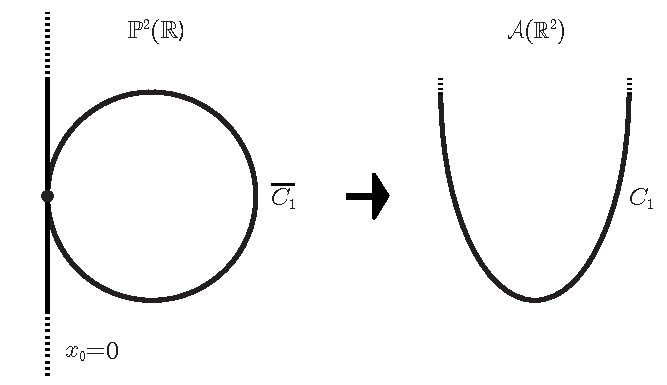
\includegraphics[trim=0cm 0cm 0cm 0cm,clip,scale=0.50]{images/projconic1.pdf}
		\end{minipage}\\
	\begin{minipage}{0.57\textwidth}
		\begin{enumerate}[resume=proj2]
		\item $\overline{C_2}$ è ‘‘\textit{disgiunta}'' dalla retta impropria.
		\end{enumerate}
	\end{minipage}
	\begin{minipage}{0.52\textwidth}
					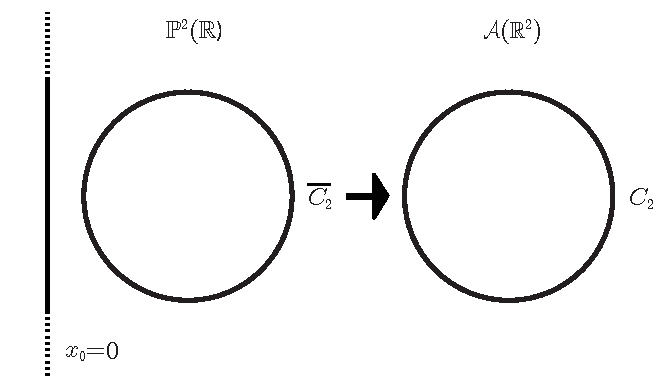
\includegraphics[trim=0cm 0cm 0cm 0cm,clip,scale=0.50]{images/projconic2.pdf}
	\end{minipage}\\
	\begin{minipage}{0.57\textwidth}
	\begin{enumerate}[resume=proj2]
		\item $\overline{C_3}$ è ‘‘\textit{secante}'' rispetto alla retta impropria.
	\end{enumerate}
\end{minipage}
\begin{minipage}{0.52\textwidth}
					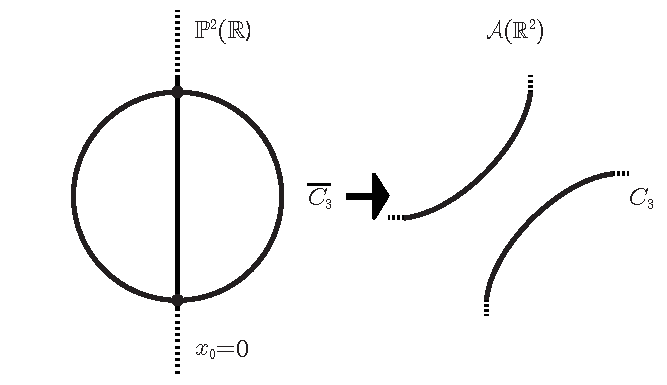
\includegraphics[trim=0cm 0cm 0cm 0cm,clip,scale=0.50]{images/projconic3.pdf}
\end{minipage}
\end{examples}
\begin{example}
	In $\aff{\realset^2}$ consideriamo la coppia di \textit{rette parallele} distinte $x(x+1)=0$ e la coppia di \textit{rette incidenti} distinte $xy=0$.\\
	Prendendo le le chiusure proiettive si ottiene $x_1(x_1+x_0)=0$ e $x_1x_2=0$, entrambe coppie di rette distinte reali in $\proj[2]{\realset}$ con segnatura (1,1). \\
	Dunque sono proiettivamente equivalenti fra loro ma hanno posizione diversa rispetto alla retta impropria.
	\begin{itemize}
		\item La prima ha un solo punto improprio $(0\colon 0\colon 1)$, che è la \textit{direzione comune} delle due rette parallele nel piano affine.
		\begin{center}
			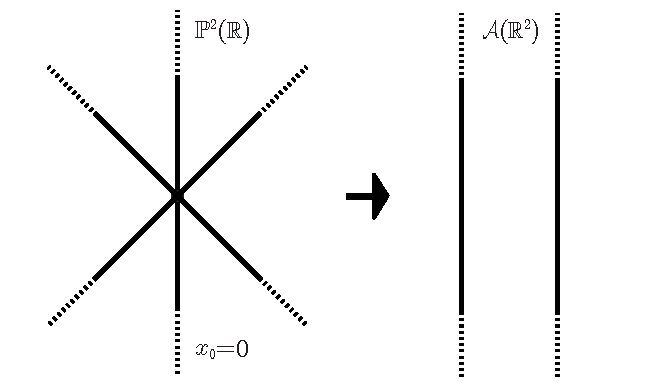
\includegraphics[trim=0cm 0cm 0cm 0cm,clip,scale=0.50]{images/projlineintersect1.pdf}
		\end{center}
		\item La seconda ha due punti impropri $(0\colon 0\colon 1)$ e $(0\colon 1\colon 0)$, che sono le direzioni delle due rette nel piano affine.
		\begin{center}
			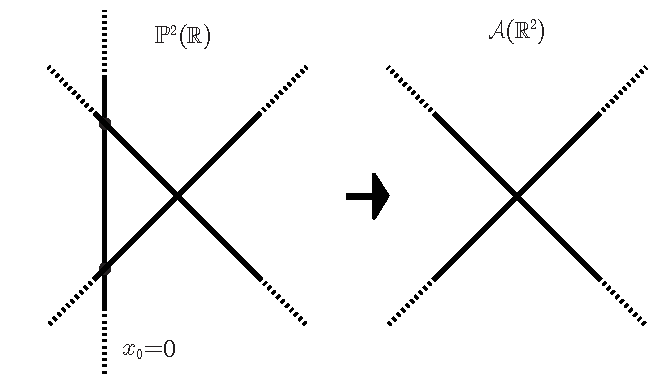
\includegraphics[trim=0cm 0cm 0cm 0cm,clip,scale=0.50]{images/projlineintersect2.pdf}
		\end{center}
	\end{itemize}
\vspace{-3mm}
\end{example}
Ragionando in questo modo dalla classificazione delle coniche proiettive si può mettere in relazione la classificazioni delle coniche affini $\aff{\realset^2}$ (a meno di rototraslazione), prestando attenzione alla posizione rispetto alla retta impropria.
\subsection{Classificazione affine delle coniche nel caso complesso}
\begin{proposition}\textsc{Classificazione delle coniche affini complesse}.
Ogni conica in $\complexset^2$ si può ridurre con una trasformazione del tipo:
\begin{equation}
	\begin{pmatrix} x' \\ y' \end{pmatrix} =A\begin{pmatrix} x \\ y \end{pmatrix} +b
\end{equation}
Con $b\in\complexset^2$ e $A\in\gl(2,\complexset)$ ad una delle cinque coniche:
\begin{center}
	\begin{tabular}{cll}
	1. &	$x^2+y^2+1=0$ & \begin{tabular}{l}
			${\scriptstyle \blacksquare}$ Rango 3.\\
			${\scriptstyle \blacksquare}$ \textit{Due} punti impropri \textit{distinti}.
		\end{tabular}   \\ \hline
	2. &	$y-x^2=0$ & \begin{tabular}{l}
			${\scriptstyle \blacksquare}$ Rango 3.\\
			${\scriptstyle \blacksquare}$ Un \textit{unico} punto improprio.
		\end{tabular}  \\ \hline
	3. &	$x^2+y^2=(x+iy)(x-iy)=0$ & \begin{tabular}{l}
			Coppia di rette distinte \textit{incidenti}:\\
			${\scriptstyle \blacksquare}$ Rango 2.\\
			${\scriptstyle \blacksquare}$ \textit{Due} punti impropri \textit{distinti}.
		\end{tabular} \\ \hline
	4. &	$x(x+1)=0$ & \begin{tabular}{l}
			Coppia di rette distinte \textit{parallele}:\\
			${\scriptstyle \blacksquare}$ Rango 2.\\
			${\scriptstyle \blacksquare}$ Un \textit{unico} punto improprio.
		\end{tabular} \\ \hline
	\begin{tabular}{l}
		\\[-3mm]
		5.
	\end{tabular} &	\begin{tabular}{l}
		\\[-3mm]
		$x^2=0$
	\end{tabular} & \begin{tabular}{l}
		\\[-3mm]
		Retta doppia
	\end{tabular} \\
	\end{tabular}
\end{center}
%	DA RIASCOLTARE
%	vediamo dove andiamo a parare:guardando la chiusura proiettiva, ho 3 ranghi possibili con la loro ir/riducibilità. Dobbamo guarare la posizione possibile rispetto alla retta allìinfinito, Siccome simao su C la chiusura proj ha solo 2 posizioni possibili: 2 punt distini o 2 punti coincidenti se irriducibili in base a 2 pt impropri o un solo. Idem per la coppia di rette al caso 			1 caso in rango 1
\vspace{-3mm}
\end{proposition}
\begin{comment}
	non la dimostriamo ma abbiamo dato una giustificazione geometrica: class a meno di proj e #punti impropri
	RECAP	
	nel piano proj nel piano proj si riduce a classificare le forme quadratiche in K^3 ed usiamo l'algebra lineare: equiv proj dal rango (3 classi) mentr ein quello reale dipende anche dalla segnatura (a meno del segno) ed abbiamo 5 classi di equiv proj di coniche nel pin proj reale
	curve alg aff e chius proj
	class affine coniche in r2 passando alla chiusura proj 
	esempi che spiegao il significato geometrico
	ellisse ierbole etc	chiusura proj stessa ma cambia pos retta impropria
	class affine coniche in c2, guardo anche il numero di punti impropri
	class coniche semplice perché è alg ineare, da grado 3 in su è meno semplice, servono dunque le nozioni per studiare curva algebrica, che sia affine o proiettiva
\end{comment}
	\subsection{Polinomi omogenei in 2 variabili}
I polinomi omogenei in \textit{due variabili} si comportano per alcuni aspetti come polinomi in \textit{una sola variabile}.\\
Sia $F\in\kamp[x_0x_1]$ un polinomio omogeneo di grado $d$, costituito da $d+1$ monomi:
\begin{equation*}
	F=a_0x_0^d+a_1x_0^{d-1}x_1+a_2x_0^{d-2}x_2^2+\ldots + a_{d-1}x_0x_1^{d-1}a_dx_1^d
\end{equation*}
Ricordiamo che vedendo $\left(x_0\colon x_1\right)\in\proj[1]{\ }$, allora $F$ ha degli zeri su $\proj[1]{\ }$, ovvero $F\left(P\right)=0$ è ben posto per $P=(a\colon b)\in\proj[1]{\ }$.
\begin{define}\textsc{Annullarsi in un punto}.\\
	Diciamo che $F$ si \textbf{annulla in } $P=(a\colon b)$ \textbf{all'ordine } $m$ se $(ax_1-bx_0)^m$\index{annullarsi in un punto} è la massima potenza di $ax_1-bx_0$ che divide $F$.
\end{define}
%		va letta ome la propr in 1 var come le radici /Ruffini!/
\begin{proposition} \label{teo polinomi omogenei 2 variabili}~{}
	\begin{enumerate}
		\item	$F$ si annulla in un punto $P=(a\colon b)\in\proj[1]{\ } \iff ax_1-bx_0\mid F$.
		\item 	Se $d=\deg F$, $F$ ha al più $d$ zeri su $\proj[1]{\ }$ contati con molteplicità. %/analogo degli zeri 
		\item	Se $F\in\complexset[x_0,\ x_1]$, allora $F$ si fattorizza come prodotto di forme lineari e ha esattamente $d$ zeri in $\proj[1]{\ }$ contati con molteplicità.\footnote{Questo punto è analogo al caso in una variabile per cui, in $\complexset$, ogni polinomio si fattorizza come prodotto di polinomi di grado 1 ed ha tutti gli zeri ben definiti.}.
	\end{enumerate}
\vspace{-3mm}
\end{proposition}
\begin{demonstration}
	% Facciamo un'ipotesi che ci semplificherà la notazione, per poi studiare il caso generale.\\
	Supponiamo che $x_0 \nmid F$; ciò è vero se e solo se $a_d\neq 0$ o, alternativamente, $F(0\colon 1)\neq 0$. Poniamo:
	\begin{equation}
		f\coloneqq F(1,t)\in\kamp[t] = a_0+a_1t+\ldots+a_{d-1}t^{d-1}+a_dt^d
	\end{equation}
	Esso è un polinomio nella sola variabile $t$, dato che abbiamo posto $x_0=1$ e $x_1=t$, ed è ancora di grado $d$ perché $a_d\neq 0\implies \deg f=\deg F=d$. Inoltre:
		\begin{itemize}
			\item $F$ è l'omogeneizzato di $f$ rispetto a $x_0$:
			\begin{equation*}
				F=x_0^2f\left( \frac{x_1}{x_0} \right)
			\end{equation*}
			\item Gli zeri di $F$ sono tutti e soli della forma $(1\colon\lambda)$ con $\lambda$ radice di $f$, dato che \textit{deomogeneizzando} passiamo da 2 variabili in 1 variabile, infatti $F(1,\lambda)=f(\lambda)$.
		\end{itemize}
	Pertanto, le proprietà di $F$ che vogliamo dimostrare seguono da quelle di $f$ che conosciamo già.
		\begin{enumerate}[label=\Roman*]
			\item $F$ si annulla in $(1\colon\lambda)=(a\colon b)$ \footnote{Con $\lambda=\frac{b}{a}$.}$\iff f(\lambda)=0 \iff t-\lambda \mid f \iff x_1-\lambda x_0\mid F$. %in particolare l'omogeneizzato divide $F$ (non ho questa nota).
			\item È immediato dal punto $1$, perché se $F$ si annulla in $P_i=(a_i\colon b_i)$ distinti con molteplicità $m_i$, allora:
			\begin{equation*}
				(a_ix_1-b_ix_0)^{m_i} \mid F,\ \forall i=1,\ \ldots,\ r 
			\end{equation*}
			Siccome i punti $P_i$ sono distinti, allora i polinomi sono \textit{primi fra loro} al variare di $i$, dunque anche il loro prodotto deve dividere $F$:
			 \begin{equation*}
			 	\prod_{i=1}^r (a_ix_1-b_ix_0)^{m_i}\mid F \implies \sum_{i=1}^r m_i\leq d=\deg F
			 \end{equation*}.
			\item Segue immediatamente dal caso complesso in una variabile; infatti, $f$ si scrive come:
			\begin{equation*}
				f=c(t-\lambda_1)^{m_1}\cdot \ldots\ \cdot (x_1-\lambda_r x_0)^{m_r}
			\end{equation*}
			Siccome $\complexset$ è algebricamente chiuso, $F=c(x_1-\lambda_1x_0)^{m_1}\cdot \ldots\cdot (x_1-\lambda_rx_0)^{m_r}$, cioè si fattorizza completamente con forma lineari. Non solo questo polinomio divide $F$ ma, a meno di costante, ho l'\textit{uguaglianza}, per cui il numero di zeri contati con molteplicità è pari al suo grado.
		\end{enumerate}
	Se invece $x_0\mid F$, allora $F=x_0^r G$ per un certo $r$, con $G$ un polinomio omogeneo di grado $d-r$ tale per cui $x_0\nmid G$. Allora i risultati trovati valgono per $G$ e, tenendo conto che $F$ si annulla in $(0\colon 1)$ con molteplicità $r$, segue la tesi della proposizione.
\end{demonstration}
\subsection{Intersezione tra una retta ed una curva nel piano proiettivo}
%Useremo queste proprietà dei polinomi omogenei di secondo grado per studiare l'intersezione fra una retta ed una curva in $\proj[2]{\ }$.\\
Sia $C$ una curva in $\proj[2]{\ }$ di grado $d$ ed equazione $F(x_0,\ x_1,\ x_2)=0$ e sia $r\subset\proj[2]{\ }$ una retta proiettiva. Vogliamo intersecare la retta $r$ con il supporto di $C$.
\begin{tips}
	Per studiare l'intersezione di due sottoinsiemi può essere comodo esprimere uno dei due sottoinsiemi in \textit{forma parametrica} e sostituire i risultati trovati nelle equazioni dell'altro.
\end{tips}
%Di uno ho le equazioni, mentre so come scrivere in forma parametrica la retta
Scriviamo una parametrizzazione per $r$; per farlo sono necessari servono 2 punti distinti $a,\ b\in r$. In questo modo, ogni punto di $r$ si scrive come combinazione lineare di altri due punti noti della retta e dei loro vettori:
\begin{equation}
	P=\lambda A+\mu B=\left[\lambda v+\mu w\right]
\end{equation}
Dove $v$ è un vettore che rappresenta $A$ ($A=[v]$) e $w$ è un rappresentante per $B$ ($A=[w]$), con $v,\ w\in\kamp^3$ e $(\lambda\colon\mu)\in\proj[1]{\ }$. Allora $C\cap r$ è dato da $F(\lambda v+\mu w)=0$; dato che vogliamo trovare il punto di intersezione descritto dai parametri $(\lambda\colon\mu)$, possiamo vedere questa sostituzione come un polinomio $G$ in $\lambda$ e $\mu$, cioè $G\left(\lambda,\ \mu\right)\in\kamp[\lambda,\ \mu]$:
\begin{equation}
	G\left(\lambda,\ \mu\right)\coloneqq F(\lambda v_0+\mu w_0,\ \lambda v_1+\mu w_1,\ \lambda v_2+\mu w_2)
\end{equation}
In particolare, abbiamo due possibilità:
	\begin{enumerate}
	\item	$r\subseteq C$: la retta è contenuta nella conica, quindi \textit{ogni punto della retta} soddisfa l'equazione; il polinomio è \textit{identicamente nullo}, ovvero $G\equiv 0$
	\item	$r\nsubseteq C$: la retta \textit{non} è contenuta nella conica, allora $G$ è un polinomio omogeneo di grado $d$ in $\lambda$ e $\mu$ le cui radici. Le radici di $G$ sono i \textit{punti di intersezione} $r\cap C$. 
\end{enumerate}
%LEZ 34
\begin{example}
	In $\proj[2]{\realset}$ sia $C\colon x_0^2+x_1^2-x_2^2=0$, $r_1\colon x_1=x_2$ e $r_2\colon x_0+x_1=0$; vogliamo calcolare le intersezioni $r_i\cap C$:
	\begin{itemize}
		\item $r_1\colon x_1=x_2 \rightarrow x_0^2=0 \text{ e } r_1\cap C=\{ (0\colon 1 \colon 1) \} \text{ molteplicità 2}$
		\item $r_2 \colon x_1=-x_0 \rightarrow 2x_0^2=x_2^2 \rightarrow x_2=\pm \sqrt{2}x_0 \ \ x_0=1\implies x_1=-1,\ x_2=\pm \sqrt{2}$\\
			$\implies \text{ due punti di intersezione } (1\colon -1\colon \sqrt{2}) \text{ e } (1\colon -1\colon -\sqrt{2})$
	\end{itemize}
\end{example}
\begin{define}\textsc{Molteplicità di intersezione}.\\
	Se $(\lambda_0\colon\mu_0)\in\proj[1]{\ }$ è una radice di $G$ di molteplicità $m$ (ovvero è il massimo esponente della forma lineare che divide $G$), allora diciamo che $C$ e $r$ hanno \textbf{molteplicità di intersezione}\index{molteplicità!di intersezione} $m$ nel punto $P=\lambda_0 A+\mu_0 B$. Poniamo:
	\begin{itemize}
		\item $m=0$ se $P\notin C\cap r$.
		\item $m=\infty$ se $P\in r$ e $r\subset C$.
	\end{itemize} 
\end{define}
\begin{observe}
	Se $r\nsubseteq C$, allora l'intersezione è finita:
	\begin{equation*}
		C\cap r=\{P_1,\ \ldots,\ P_n\}
	\end{equation*}
	Sia $m_i$ la molteplicità di intersezione in $P_i$; il numero di questi punti di intersezione è minore del grado della curva:
		\begin{equation}
			\# (C\cap r)\leq \deg C
		\end{equation}
	Più precisamente, $\displaystyle \sum_{i=1}^n m_i\leq\deg C$; infatti, le radici di $G\left(\lambda,\ \mu\right)=0$ danno i punti di intersezione della curva con la retta e può avere al più $d$ soluzioni, tante quante il grado della curva (anche se contate con molteplicità per la proposizione \ref{teo polinomi omogenei 2 variabili}).\\
	Se $\kamp=\complexset$, possiamo dire che la somma delle molteplicità è esattamente $d$:
	\begin{equation}
		\displaystyle \sum_{i=1}^n m_i=\deg C
	\end{equation}
	In particolare, la retta e la curva si intersecano \textit{sempre} nel \textit{piano proiettivo complesso}, ovvero $C\cap R\neq 0$.\\
	Se $\kamp=\realset$ e $d$ è \textbf{dispari} allora possiamo ancora concludere che la retta e la curva si intersecano sempre in quanto $G$ deve annullarsi almeno in un punto reale, e quindi $C\cap r\neq 0$.
\end{observe}
\begin{example}
	Se $C\subset\proj[2]{\complexset}$ è una conica ($\deg C=2$) ed $r$ è una retta non contenuta in $C$, ovvero $r\nsubseteq C$, allora:
	\begin{equation}
		r\cap C=\hspace{-2mm}\begin{array}{ll}
			\nearrow &\{2\text{ punti con molteplicità } 1\}\\
			\searrow & {\{1 \text{ punto con molteplicità } 2\}}
		\end{array}
	\end{equation}
	% https://q.uiver.app/?q=WzAsMyxbMCwxLCJyXFxjYXAgQz0iXSxbMiwwLCJcXHsyXFx0ZXh0eyBwdW50aSBjb24gbW9sdGVwbGljaXTDoCB9IDFcXH0iXSxbMiwyLCJcXHsxIFxcdGV4dHsgcHVudG8gY29uIG1vbHRlcGxpY2l0w6AgfSAyXFx9Il0sWzAsMl0sWzAsMV1d
	Se la conica $C\subset\proj[2]{\realset}$ ed $r$ è una retta non contenuta in $C$, ovvero $r\nsubseteq C$, allora c'è \textit{anche} la possibilità che l'intersezione sia \textit{vuota}, cioè $C\cap r=\emptyset$ (ad es. $C\colon x_0^2+x_1^2-x_2^2=0$ e $r_3\colon x_2=0$).
\end{example}
	
\begin{tips}
	Se una conica $C$ contiene tre punti \textit{allineati}, allora $C$ contiene una retta, è riducibile (l'equazione della retta divide quella della conica)e $\rk C\leq 2$.		
\end{tips}
\begin{observe} 	Si può dimostrare che:
	\begin{enumerate}
		\item La molteplicità di intersezione fra $C$ e $r$ in $P$ non dipende dalla parametrizzazione scelta per $r$.
		\item La molteplicità di intersezione è \textbf{invariante} per \textit{proiettività}.
	\end{enumerate}
\vspace{-3mm}
\end{observe}
\begin{demonstration} Dimostriamo l'ultimo punto
	Sia $\funz f {\proj[2]{\ }} {\proj[2]{\ }}$ una proiettività e $C'$ la trasformata di $C$ tramite $f$ con $C\colon F(x_0,\ x_1,\ x_2)=0$ e $f\colon x'=Mx$. Allora $f^{-1}\colon x=M^{-1}x'$ e $C'\colon F'(x')=F(M^{-1}x')=0$ è un polinomio omogeneo di grado $d$.\\
	Le proiettività portano curve algebriche in curve algebriche, ovvero $r'=f(r)$ è una retta e $P'=f\left(P\right)$. Pertanto, la molteplicità di intersezione fra $C$ e $r$ in $P$ è uguale alla molteplicità di intersezione fra $C'$ e $r'$ in $P'$.
\end{demonstration}
\subsection{Intersezione tra una retta ed una curva nel caso affine}
Sia $C$ una curva in $\kamp^2$ di equazione $f\left(x,\ y\right)=0$ e sia $r$ una retta affine. Scegliamo una parametrizzazione per $r$:
\begin{equation}
	r\colon\begin{cases}
	x=tv_1+w_1\\
	y=tv_2+w_2
\end{cases}
\end{equation}
Per intersecare $C$ ed $r$ sostituiamo la parametrizzazione di $r$ nell'equazione di $C$ ed otteniamo un polinomio nell'unico parametro $t$:
\begin{equation}
	g(t)\coloneqq f(tv_1+w_1,\ tv_2+w_2)\in\kamp[t]
\end{equation}
In modo analogo al caso proiettivo, le radici di $g$ corrispondono ai \textit{punti di intersezione} e definiamo la \textbf{molteplicità di intersezione} di $C$ ed $r$ in un punto $P=t_0v+w$ come la molteplicità di $t_0$ come radice di $g(t)$.\\
\begin{observes}~{}
		\begin{enumerate}
		\item	La molteplicità di intersezione non dipende dalla scelta di parametrizzazione della retta $r$.
		\item	La molteplicità di intersezione è \textbf{invariante} per \textit{affinità}.
		\item	La \textit{molteplicità affine} è pari a quella proiettiva. Per precisare, sia $P\in C\cap r$, $\overline{C}$ la chiusura proiettiva di $C$ in $\proj[2]{\ }\supset\kamp^2$ ed $\overline{r}$ la chiusura proiettiva di $r$ in $\proj[2]{\ }$; allora la molteplicità di intersezione tra $C$ e $r$ in $P$ è uguale alla molteplicità di intersezione fra $\overline{C}$ e $\overline{r}$ in $P$.
	\end{enumerate}
\vspace{-3mm}
\end{observes}
\subsection{Retta tangente}
\begin{define}\textsc{Retta tangente ad una curva in un punto}\\
Sia $C$ una curva piana (affine o proiettiva) ed $r$ una retta (affine o proiettiva). Diciamo che $r$ è \textbf{tangente} \index{retta!tangente} a $C$ in un punto $P$ se la \textit{molteplicità di intersezione} fra $C$ ed $r$ in $P$ è \textit{maggiore di 1}.
\end{define}
\begin{example}	Sia $C$ in $\proj[2]{\realset}$ una conica di equazione $x_0^2+x_1^2-x_2^2=0$ e una retta di equazione $r_1\colon x_1-x_2=0$; poiché l'intersezione è solo il punto $r_1\cap C=\{(0\colon 1\colon 1)\}=P$, allora $r_1$ è tangente a $C$ in $P$ e ‘‘coincide'' con la tangente nel senso geometrico.\\
La conica $C_1$ in $\aff{\realset^2}$ si ottiene deomogeneizzando $C$ rispetto alla variabile \textit{non} nulla $x_2$ (in questo caso in $P$ si ha che $x_0=0$), per cui:
\begin{equation*}
		x=\frac{x_0}{x_2}\quad y=\frac{x_1}{x_2}
	\end{equation*}
	Dunque $C_1$ ha equazione:
	\begin{equation*}
		\left( \frac{x_0}{x_2} \right)^2 + \left( \frac{x_0}{x_2} \right)^2 -1 =0
	\end{equation*}
\begin{minipage}{0.75\textwidth}
È pari quindi alla circonferenza $x^2+y^2=1$ con $P=(0,\ 1)$. In questo caso la tangente in $P$ è chiaramente la retta $y=1$.\\
Passando alle coordinate proiettive diventa $\frac{x_1}{x_2}=1 \implies x_1=x_2$. Notiamo come la \textit{chiusura proiettiva} della \textit{tangente affine} sia proprio la \textit{tangente proiettiva}.
\end{minipage}
\hspace{-12mm}
\begin{minipage}{0.24\textwidth}
	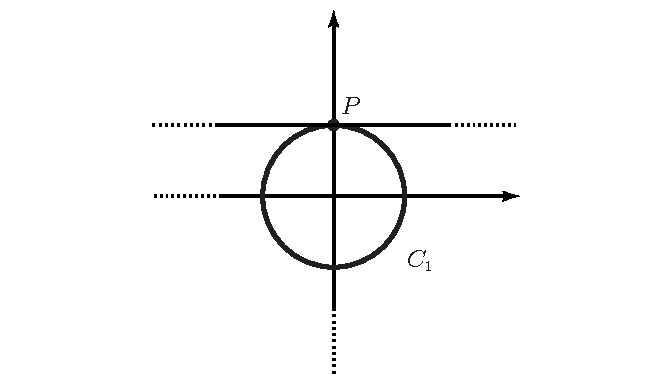
\includegraphics[trim=0cm 0cm 0cm 0cm,clip,scale=0.50]{images/planecurve1.pdf}
\end{minipage}
\end{example}
\begin{example} \label{esempiocurvaq}	Sia $C$ in $\aff{\realset^2}$ la curva di equazione $f\ \colon y^2=x^2+x^3=x^2(x+1)$, una \textbf{cubica} in quanto ha grado 3.\\
Vogliamo calcolare quali sono le rette tangenti nel punto $P=(-1,\ 0)\in C$. Consideriamo pertanto il fascio di rette passanti per $P$ e le intersechiamo con la cubica per determinare quali sono tangente con la definizione; guardiamo dunque quali hanno molteplicità di intersezione maggiore di 1.\\
Il fascio di rette per $P$ è:
\begin{equation*}
	r\colon \begin{cases}
		x=-1+tv_1\\
		y=tv_2
	\end{cases}
\end{equation*}
Con $(v_1,\ v_2)$ direzione di $r$. Sostituiamo la parametrizzazione di $r$ nell'equazione di $C$, costruendo la funzione $g\left(t\right)$:
	\begin{gather*}
		t^2v^2=(tv_1-1)^2 tv_1\\
		g(t)=(tv_1-1)^2tv_1-t^2v_2^2=t[v_1(t^2v_1^2+1-2tv_1)-tv_2^2]=t[v_1^3t^2-t(2v_1^2+v_2^2)+v_1]
	\end{gather*}
	Analizziamo cosa abbiamo trovato:
		\begin{itemize}
			\item $t=0$ è sempre una soluzione: per costruzione abbiamo preso la retta che passava per $P$, dunque $P$ è banalmente intersezione di una retta di \textit{qualsiasi} direzione con la cubica.
			\item La molteplicità di intersezione fra $C$ e $r$ in $P$ è la massima potenza di $t$ che divide $g$; pertanto è $m$ se $t^m$ è la massima potenza di $t$ che divide $g$.\\
			In questo caso, quand'è che la molteplicità di intersezione è maggiore di 1? Nell'equazione che abbiamo scritto almeno $t^2$ deve dividere $g$: l'unica possibilità per questa curva di poter raccogliere un'altro $t$ è avere $v_1=0$. Allora $r$ è la retta verticale che passa per $P$ e abbiamo determinato che esiste ed è l'\textit{unica} tangente in $P$.
		\end{itemize}
	Vediamo ora un caso in cui la retta tangente ad un punto non è unica. Consideriamo la stessa cubica ma \textit{cambiamo il punto}, prendendo l'origine $Q=\left(0,\ 0\right)\in C$.\\
	Scriviamo il fascio di rette per $Q$:
	\begin{equation*}
		q\colon \begin{cases}
			x=tw_1\\
			y=tw_2
		\end{cases}
	\end{equation*}
	Con $(w_1,\ w_2)$ direzione. Analogamente a prima:
	\begin{gather*}
		h(t)=t^2w_1^2+t^3w_1-t^2w_2^2=t^2(w_1^2-w_2^2+tw_1^3)
	\end{gather*}
\begin{minipage}{0.75\textwidth}
Troviamo così che $t^2$ si può sempre raccogliere, dunque in questo caso la molteplicità di intersezione fra le rette e $Q$ è sempre almeno 2. In particolare, ogni retta per $Q$ ha intersezione maggiore di 2, dunque è \textit{tangente}.\\
Osserviamo che nel punto $Q$ la curva si auto-interseca: ogni retta per l'origine interseca la curva almeno due volte, quindi è tangente. Fra queste, ci sono due \textit{direzioni speciali} per cui la molteplicità è 3:
\begin{itemize}
	\item $w_1^2-w_2^2=0\implies w_1=w_2 \implies \mathcal{L}(1,1) \colon y=x$.
	\item $w_1=-w_2 \implies \mathcal{L}(1,-1) \colon y=-x$.
\end{itemize}
\end{minipage}
\hspace{-12mm}
\begin{minipage}{0.24\textwidth}
	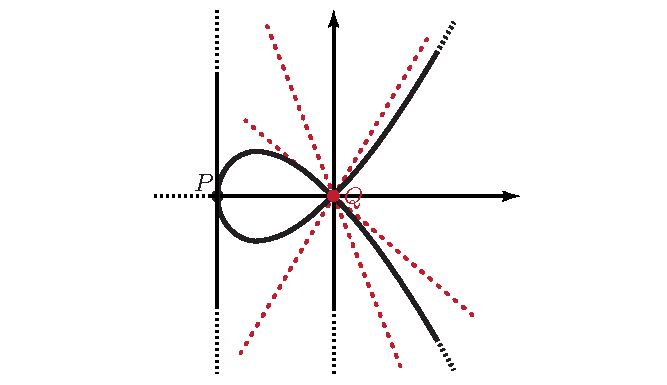
\includegraphics[trim=0cm 0cm 0cm 0cm,clip,scale=0.50]{images/planecurve2.pdf}
\end{minipage}
\end{example}
\subsubsection{Caso affine}
Sia $C\colon f\left(x,\ y\right)=0$ in $\kamp^2$ e $P=(x_0,\ y_0)$. Osserviamo che possiamo sempre scrivere il polinomio come un polinomio centrato in $x_0,\ y_0$, cioè come polinomio in $x-x_0$ e $y-y_0$ invece che come polinomio in $x$ e $y$.
\begin{gather*}
		f=\sum_{i,j\geq 0} a_{ij}x^iy^j = \sum_{i,j\geq 0} a_{ij}(x-x_0+x_0)^i(y-y_0+y_0)^j \stackrel{!}{=} 	\sum_{i,j\geq 0}b_{ij}(x-x_0)^i(y-y_0)^j\\
		\implies f(x_0,\ y_0)=b_{00}=f\left(P\right) \implies f=f\left(P\right) +\alpha (x-x_0)+\beta (y-y_0)+ \text{ termini di grado} >1
\end{gather*}
Nel passaggio indicato con (!) si stanno sottintendendo conti con il binomio di Newton.\\
\begin{define}\textsc{Derivate parziali}.\\
	Dato un polinomio $f=\sum_{i,j}a_{ij}x^iy^j\in\kamp[x,\ y]$, le \textbf{derivate parziali}\index{derivata!parziale} di $f$ sono i seguenti polinomi:
	\begin{equation}
		\frac{\partial{f}}{\partial{x}}\coloneqq \sum_{i,j}a_{ij}ix^{i-1}y^j\quad \frac{\partial{f}}{\partial{y}}\coloneqq \sum_{i,j}a_{ij}jx^iy^{j-1}
	\end{equation}
\vspace{-3mm}
\end{define}
Si verifica che $\alpha=\frac{\partial{f}}{\partial{x}}(x_0,\ y_0)$ e $\beta=\frac{\partial{f}}{\partial{y}}(x_0,\ y_0)$.
\begin{demonstration}
	Se $P\in C$, segue dai ragionamenti precedenti $f=\alpha (x-x_0)+\beta (y-y_0)+ \text{ termini di grado} >1$. Applicando la definizione di derivata parziale si hanno:
	\begin{equation*}
		\frac{\partial{f}}{\partial{x}}= \sum_{i,j}a_{ij}i\left(x-x_0\right)^{i-1}\left(y-y_0\right)^j\quad \frac{\partial{f}}{\partial{y}}= \sum_{i,j}a_{ij}j\left(x-x_0\right)^i\left(y-y_0\right)^{j-1}
	\end{equation*}
	Valutando in $P=(x_0,\ y_0)$:
	\begin{equation*}
		\frac{\partial{f}}{\partial{x}}\left(P\right)=a_{10}=\alpha\quad \frac{\partial{f}}{\partial{y}}\left(P\right)=a_{01}=\beta
	\end{equation*}
\end{demonstration}
%LEZ 35
\begin{define}\textsc{Gradiente}.\\
	Il \textbf{gradiente}\index{gradiente} $\nabla f$ è il vettore con componenti le derivate parziali:
	\begin{equation}
		\nabla f=\left( \frac{\partial{f}}{\partial{x}},\ \frac{\partial{f}}{\partial{y}} \right)
	\end{equation}
\vspace{-6mm}
\end{define}
Il gradiente valutato in $P=(x_0,\ y_0)$ è $\nabla f\left(P\right)=(\alpha,\beta)\in\kamp^2$.\\
%Adesso vogliamo intersecare con l retta genereica per P
\paragraph{Tangente e derivate parziali}
Sia $r$ la retta per $P$ con direzione $v=(v_1,v_2)$ e descrizione parametrica:
\begin{equation*}
	\begin{cases}
		x=x_0+tv_1\\
		y=y_0+tv_2
	\end{cases}
\end{equation*}
Allora:
	\begin{equation*}
		\begin{array}{ll}
			g(t)=f(x_0+tv_1,\ y+tv_2)&=\alpha tv_1+\beta tv_2 + \text{ termini in }t\text{ di grado }\geq 2 =\\
			&= (\alpha v_1+\beta v_2)t + \text{ termini in }t \text{ di grado }\geq 2
		\end{array}	
	\end{equation*}
Si hanno dunque due possibilità, che dipendono dal coefficiente di $t$:
	\begin{enumerate}
		\item	$\alpha=\beta=0$, ovvero $\nabla f =0$: il \textit{coefficiente} è nullo indipendentemente dalla retta. Allora, $\forall r$ retta per $P$,  $t^2 \mid g(t)$: la molteplicità di intersezione è $\geq 2$ e \textit{ogni} retta per $P$ è tangente a $C$ in $P$.
		\item	$\nabla f\left(P\right)=(\alpha,\beta)\neq 0$:	il coefficiente di $t$ determina in maniera \textit{univoca} la direzione della retta, che è quella \textbf{ortogonale} a $(\alpha,\beta)$. Ciò implica che $\exists !$ retta tangente a $C$ in $P$ ed è quella di direzione $(-\beta,\alpha)$ con equazione	$\alpha(x-x_0)+\beta(y-y_0)=0$, ovvero 
			\begin{equation}
				\frac{\partial{f}}{\partial{x}}\left(P\right)(x-x_0) + \frac{\partial{f}}{\partial{y}} \left(P\right)(y-y_0)=0
			\end{equation}
	\end{enumerate}
% Abbiamo così ritrovato la casistica della cubica con i punti espliciti: ogni retta è tangente oppure c'è una sola tangente alla curva nel punto.
\begin{define}\textsc{Punto singolare}.\\
	Sia $C$ una curva affine in $\kamp^2$ di equazione $f\left(x,\ y\right)=0$. Un punto $P\in C$ è detto \textit{non singolare} o \textbf{liscio}\index{punto!liscio} se $\nabla f\left(P\right)\neq 0$. Altrimenti $P$ è detto \textbf{punto singolare} \index{punto!singolare}.\\
	Una curva $C$ è detta \textbf{singolare} se ha almeno un punto singolare, altrimenti è detta curva \textit{non singolare} o \textbf{liscia}.
\end{define}
Abbiamo visto prima che se $P$ è \textit{non singolare} esiste ed è unica la tangente a $C$ in $P$. Essa ha equazione	$\frac{\partial{f}}{\partial{x}}\left(P\right)(x-x_0) + \frac{\partial{f}}{\partial{y}} \left(P\right)(y-y_0)=0$ e, essendo non singolare, almeno uno dei due coefficienti non è nullo.\\
Se invece $P$ è \textit{singolare} allora ogni retta per $P$ è tangente a $C$ in $P$.
\subsubsection{Caso proiettivo}
Vogliamo analizzare la tangenza nel \textit{caso proiettivo}. Tuttavia, prima di trattare di punti singolare o tangenti, ci servirà una proprietà dei polinomi omogenei, detta \textbf{relazione di Eulero} sui polinomi omogenei. Essa vale per un qualsiasi \textit{numero di variabili} a coefficienti in un campo \textit{qualsiasi} e mette in relazione un polinomio omogeneo con sue derivate parziali, che per costruzione sono polinomi omogenei di un \textit{grado inferiore}.
\begin{theorema}\textsc{Relazione di Eulero} \index{Relazione!di Eulero} \\
	Sia $F\in\kamp[x_0,\ \ldots,\ x_n]$ polinomio omogeneo di grado $m$ e le sue derivate parziali $\frac{\partial{f}}{\partial{x_i}}\in\kamp[x_0,\ \ldots,\ x_n]$, polinomio omogenei di grado $m-1$. Si ha che:
		\begin{equation}
			\sum_{i=0}^n x_i\frac{\partial{F}}{\partial{x_i}}=mF
		\end{equation}
	\vspace{-6mm}
\end{theorema}
Nella relazione appena annunciata notiamo che moltiplichiamo ciascuna derivata parziale per $x_i$. Ciò è necessario per la \textit{buona definizione} dell'equazione: siccome le derivate parziali sono omogenee di grado $m-1$, moltiplichiamo per $x_i$ affinché la somma sia omogenea di grado $m$ come il polinomio $F$.
\begin{demonstration}
	Basta mostrarlo per un monomio $G=\lambda x_0^{j_0}\cdots x_n^{j_n}$ con $j_0+\ldots+j_n=m,\ \lambda\in\kamp$. Scrivendone le derivate parziali rispetto ad una variabile e poi moltiplicando per $x_i$ sistemiamo l'esponente $i$-esimo:
		\begin{gather*}
			\frac{\partial{G}}{\partial{x_i}}=\lambda j_i x_0^{j_0}\ldots x_i^{j_{i-1}} \ldots x_n^{j_n} \implies  x_i \frac{\partial{G}}{\partial{x_i}}=\lambda j_i x_0^{j_0}\ldots x_i^{j_i} \ldots x_n^{j_n}\\
			\implies \sum_{i=0}^n x_i\frac{\partial{G}}{\partial{x_i}} = \sum_{i=0}^n \lambda j_i x_0^{j_0} \ldots x_n^{j_n}=\lambda x_0^{j_0}\ldots x_n^{j_n} \cdot \sum_{i=0}^n j_i =mG
		\end{gather*}
\end{demonstration}
%il monomio è sempre lo stesso perché si moltiplica per x_i
%monomio j e somma degli esponenti è esattamente di grado, dunque =mG
%sing e non sing rette tang per piane pro
\begin{proposition}
	Sia $C$ in $\proj[2]{\ }$ una curva di equazione $F\left(x_0,\ x_1,\ x_2\right)=0$ con $F$ polinomio omogeneo di grado $d$ e $P\in C$. $P$ è \textit{non singolare} se e solo se almeno una delle derivate parziali di F non è nulla in $P$, cioè $\exists i\in\{0,1,2\}\colon \frac{\partial{F}}{\partial{x_i}}\left(P\right)\neq 0$.\\
%allo stesso mod del caso affine con le der in p
	In tal caso esiste ed è unica la retta tangente a $C$ in $P$ ed ha equazione:
		\begin{equation}
			\underbrace{\frac{\partial{F}}{\partial{x_0}}\left(P\right) }_{\in\kamp}x_0 + \underbrace{\frac{\partial{F}}{\partial{x_1}}\left(P\right) }_{\in\kamp}x_1 + \underbrace{\frac{\partial{F}}{\partial{x_2}}\left(P\right) }_{\in\kamp}x_2 
		\end{equation}
	I cui coefficienti sono le derivate parziali di $F$ valutate in $P$.
\end{proposition}
\begin{demonstration}
	% Dobbiamo verificare che per la curva affine di cui $C$ è chiusura proiettiva (ottenuta deomogeneizzando rispetto a $x_0$) si ritrova la retta tangente affine.\\
	A meno di proiettività possiamo supporre che $P=(1\colon a\colon b)\in U_0=\{x_0\neq 0\}$, cioè che stia nella carta affine $U_0$ identificata a $\aff{\kamp^2}$: $P$ corrisponde a $\left(a,\ b\right)\in\aff{\kamp^2}$.\\
	Poniamo $f\left(x,\ y\right)\coloneqq F(1,\ x,\ y)$ e sia $C_0$ la curva in $\aff{\kamp^2}$ di equazione $f\left(x,\ y\right)=0$ per cui $C$ è la chiusura proiettiva. Mettiamo in relazione le derivate parziali di $f$ con quelle $F$ a partire dalla definizione stessa di $f$, 
%	che ci dice che facendo la derivate parziali di $f$ rispetto a $x$ è la sessa di 	valutata in	come polinomio, idem y, ed è una relazione fra polinomi
	valutandole nel punto:
		\begin{gather*}
			\begin{cases}
				\frac{\partial{f}}{\partial{x}} = \frac{\partial{F}}{\partial{x_1}} (1,\ x,\ y)\\
				\frac{\partial{f}}{\partial{y}} = \frac{\partial{F}}{\partial{x_2}} (1,\ x,\ y)
			\end{cases}
			\implies \textcolor{green}{\circled{\ast}}\quad
			\begin{cases}
				\frac{\partial{f}}{\partial{x}}\left(a,\ b\right) = \frac{\partial{F}}{\partial{x_1}} \left(1,\ a,\ b\right)\\
				\frac{\partial{f}}{\partial{y}}\left(a,\ b\right) = \frac{\partial{F}}{\partial{x_2}} \left(1,\ a,\ b\right)
			\end{cases}
		\end{gather*}
	Valutiamo la relazione di Eulero sui polinomi omogenei in $\left(1,\ a,\ b\right)$:
		\begin{gather*}
			\frac{\partial{F}}{\partial{x_0}}\left(1,\ a,\ b\right) + a\frac{\partial{F}}{\partial{x_1}}\left(1,\ a,\ b\right) + b\frac{\partial{F}}{\partial{x_2}}\left(1,\ a,\ b\right)= dF\left(1,\ a,\ b\right)=0
		\end{gather*}
	Si ha $F\left(1,\ a,\ b\right)=0$ perché $P\in C$. Riusciamo così a esprimere la derivata parziale rispetto a $x_0$ in funzione delle altre due:
		\begin{gather*}
			\textcolor{green}{\circled{\ast\ast}}\quad \frac{\partial{F}}{\partial{x_0}}=-a\frac{\partial{F}}{\partial{x_1}} -b\frac{\partial{F}}{\partial{x_2}}
		\end{gather*}
	Ne consegue che $\nabla f\left(a,\ b\right)=0 \iff  \nabla F\left(1,\ a,\ b\right)=(0,0,0)$; infatti, se il gradiente $\nabla f$ si annulla in $P$ allora si annullano le derivate parziali di $F$ rispetto a $x_1,\ x_2$, pertanto per la relazione di Eulero anche la terza derivata parziale si annulla. Viceversa, se il gradiente di $F$ si annulla bastano le relazioni $\textcolor{green}{\circled{\ast}}$ per avere che anche il gradiente di $f$ si annulla.\\
	Dunque, il punto $P$ è \textit{non singolare} se e solo se $\nabla F\left(1,\ a,\ b\right)\neq \mathbf{0}$, verificando la prima parte della proposizione.\\
	Supponendo $P$ non singolare, allora la retta tangente affine a $C_0$ in $P$ ha equazione:
	\begin{equation*}
		\frac{\partial{f}}{\partial{x}}\left(a,\ b\right)(x-a) + \frac{\partial{f}}{\partial{y}}\left(a,\ b\right)(y-b)=0
	\end{equation*}
	La chiusura proiettiva di tale retta affine dà la retta tangente proiettiva a $C$ in $P$:
	\begin{equation*}
		\frac{\partial{f}}{\partial{x}}\left(a,\ b\right)(x_1-ax_0) + \frac{\partial{f}}{\partial{y}}\left(a,\ b\right)(x_2-bx_0)=0 
	\end{equation*}
	Per $\textcolor{green}{\circled{\ast}}$ si ha che
		\begin{equation*}
			\begin{array}{ll}
				&\frac{\partial{F}}{\partial{x_1}}\left(1,\ a,\ b\right)(x_1-ax_0) + \frac{\partial{F}}{\partial{x_2}}\left(1,\ a,\ b\right)(x_2-bx_0)=0 \\[3mm]
				\implies & \underbrace{ \left( -a\frac{\partial{F}}{\partial{x_1}}\left(1,\ a,\ b\right) -b \frac{\partial{F}}{\partial{x_2}}\left(1,\ a,\ b\right) \right)}_{\textcolor{green}{\circled{\ast\ast}}}  x_0 + \frac{\partial{F}}{\partial{x_1}}\left(1,\ a,\ b\right) x_1 + \frac{\partial{F}}{\partial{x_2}}\left(1,\ a,\ b\right) x_2=0 \\
				\implies & \frac{\partial{F}}{\partial{x_0}}\left(P\right) x_0 + \frac{\partial{F}}{\partial{x_1}}\left(P\right) x_1 + \frac{\partial{F}}{\partial{x_2}}\left(P\right) x_2
			\end{array}
		\end{equation*}
\end{demonstration}

\begin{observe} \textsc{Rette tangenti: spazio affine e spazio proiettivo a confronto.}\\
	Se $C$ è una curva affine di equazione $f\left(x,\ y\right)=0$, per trovare i punti singolare di $C$ bisogna risolvere un sistema con l'equazione della curva e le derivate parziali di $f$. L'equazione della curva è necessaria perché potrei avere punti in cui il gradiente si annulla ma \textit{non} appartengono alla curva!\\ 
	Invece, se $C$ è una curva proiettiva di equazione $F\left(x_0,\ x_1,\ x_2\right)=0$, per trovare i punti singolari di $C$ bisogna solo risolvere il sistema delle derivate parziali nulle e \textit{non serve} mettere anche l'equazione della curva per via della relazione di Eulero. Infatti, se $P$ annulla $\nabla F$, allora dalla relazione di Eulero si ha che:
		\begin{equation*}
			F\left(P\right)=\frac{1}{d}\left( a\frac{\partial{F}}{\partial{x_0}}\left(P\right) + b\frac{\partial{F}}{\partial{x_1}}\left(P\right) + c\frac{\partial{F}}{\partial{x_2}}\left(P\right) \right) = 0 \implies P\in C
		\end{equation*}
	Riassumendo, ecco i sistemi a confronto:
		\begin{center}
			\begin{tabular}{c|c}
				Affine & Proiettivo \\
				\hline
				$\displaystyle \begin{cases} 
					f\left(x,\ y\right)=0 \\		\frac{\partial{f}}{\partial{x}}\left(x,\ y\right)=0\\	\frac{\partial{f}}{\partial{y}}\left(x,\ y\right)=0
				\end{cases}$ & $\displaystyle \begin{cases}
					\frac{\partial{F}}{\partial{x_0}}=0\\	\frac{\partial{F}}{\partial{x_1}}=0\\	\frac{\partial{F}}{\partial{x_2}}=0 
				\end{cases}$
			\end{tabular}
		\end{center}
\end{observe}

\begin{examples} \label{esempi lez 35}
	\begin{enumerate}
		\item	Sia $C_0\colon x^2+x^3-y^2=0$ una curva affine e $C$ la chiusura proiettiva di $C_0$ con equazione $F=x_0x_1^2+x_1^3-x_0x_2^2$. Cerchiamo i punti singolari:
			\begin{gather*}
				\nabla F=0 \iff \begin{cases}
					\frac{\partial{F}}{\partial{x_0}}=x_1^2 - x_1^2=0\\
					\frac{\partial{F}}{\partial{x_1}}=2x_0x_1+3x_1^2=0\\
					\frac{\partial{F}}{\partial{x_2}}-2x_0x_2=0
				\end{cases} \implies \begin{cases}
					x_0=0 \\ x_1=0 \\ x_2=0
				\end{cases} \text{ oppure } \begin{cases}
					x_0=t \\ x_1=0 \\ x_2=0
				\end{cases}
			\end{gather*}
		Il primo non è lecito nel piano proiettivo, dunque $P=(1\colon 0\colon 0)$ è l'unico punto singolare di $C$ e osserviamo che corrisponde a $(0,\ 0)\in\kamp^2$.\\
		A pagina \pageref{esempiocurvaq} avevamo visto il punto $Q=(-1,\ 0)\in C_0$, nel quale la curva affine si auto-intersecava; passando alla chiusura proiettiva, $Q=(1\colon -1\colon 0)\in C$ è \textit{non} singolare. Scriviamo la tangente $T_Q C$ grazie alle derivate parziali:
		\begin{equation*}
			\frac{\partial{F}}{\partial{x_0}}\left(Q\right)=1,\ \frac{\partial{F}}{\partial{x_1}}\left(Q\right)=(2x_0x_1+3x_1^2)\left(Q\right)=1,\ \frac{\partial{F}}{\partial{x_2}}\left(Q\right)=(-2x_0x_1)\left(Q\right)=0
		\end{equation*}
		Ne segue che $T_Q C\colon x_0+x_1=0$. Per ottenere la retta affine associata basta porre $x_0=1$, da cui $T_Q C_0\colon x+1=0$, perfettamente coerente con lo studio fatto nel caso affine.\\
		Avevamo visto che nel punto singolare $P=(1\colon 0\colon 0)$, tutte le rette per esso hanno molteplicità di intersezione $2$ con la curva $C$ in $P$, eccetto due rette speciali di direzione $(1,\ \pm 1)$ in cui la molteplicità di intersezione è 3. $P$ è detto \textbf{nodo}. 
		\item	Consideriamo la curva affine $C_0$ data da $f\left(x,\ y\right)=y^2-x^3$ e la chiusura proiettiva $C$ di equazione $F(x_0,\ x_1,\ x_2)=x_0x_2^2-x_1^3$. Siccome:
		\begin{equation*}
			\frac{\partial{F}}{\partial{x_0}} =x_2^2,\ \frac{\partial{F}}{\partial{x_1}}= -3x_1^2,\ \frac{\partial{F}}{\partial{x_2}}= 2x_0x_2
		\end{equation*} 
		Allora $P=(1\colon 0\colon 0)$ è l'unico punto singolare di $C$, che corrisponde all'origine di $\aff{\kamp^2}$. Consideriamo il fascio di rette per l'origine in $\aff{\kamp^2}$ e vediamo qual è la molteplicità di intersezione. Sia la generica retta per l'origine:
		\begin{equation*}
			r\colon \begin{cases}
				x=tv_1 \\
				y=tv_2
			\end{cases}\text{ con } v=(v_1,\ v_2)\text{ direzione di }r
		\end{equation*}
		La intersechiamo con $C_0$:
		\begin{equation*}
			g(t)=t^2v_2^2 -t^3v_1^3=0 \implies t^2(v_2^2 -tv_1^3)=0
		\end{equation*}
		Segue che la molteplicità di intersezione in $P$ è 2 se $v_2\neq 0$ ed è 3 se $v_2=0$.
		\begin{minipage}{0.65\textwidth}
			Si noti che i risultati ottenuti sono simili al caso precedente: la differenza sta nel fatto che quasi tutte le rette hanno molteplicità 2 e c'è solo un'unica retta con molteplicità 3 e non \textit{due} come nel caso precedente.\\
			Disegnando la curva affine si nota dunque la presenza di una \textbf{cuspide}.
		\end{minipage}
		\hspace{-12mm}
		\begin{minipage}{0.34\textwidth}
			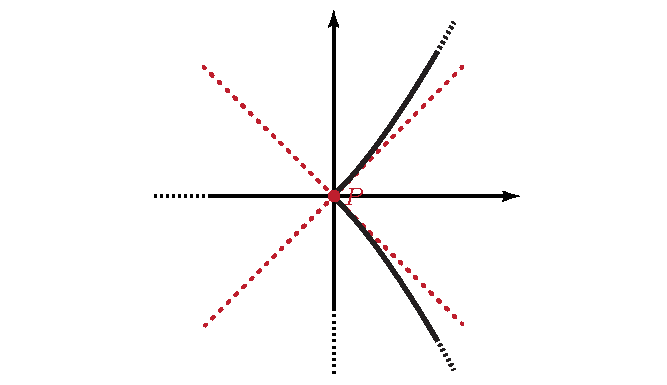
\includegraphics[trim=0cm 0cm 0cm 0cm,clip,scale=0.50]{images/planecurve3.pdf}
		\end{minipage}
	\end{enumerate}
\end{examples}
\begin{observe} \textsc{Punti singolari delle coniche.}\\
	Sia $C$ una conica proiettiva. Il \textit{numero} di punti singolari dipende solo dal \textit{rango}:
		\begin{itemize}
			\item	$\rk C=3\implies C$ \textit{non} ha punti singolari.
			\item	$\rk C=2 \implies C$ ha \textit{un} punto singolare.
			\item	$\rk C=1 \implies C$ è una \textit{retta doppia} e \textit{ogni punto} di $C$ è singolare.
		\end{itemize}
	Infatti, sia $A$ la matrice simmetrica associata a $C$, allora l'equazione associata a $C$ e le derivate parziali sono:
		\begin{gather*}
			F=X^tAX=\sum_{i,j=0}^2 a_{ij}x_ix_j \implies \frac{\partial{F}}{\partial{x_h}} = \sum_{\stackrel{j=0}{\left(i=h\right)}}^2 a_{hj}x_j+ \sum_{\stackrel{i=0}{\left(j=h\right)}}^2  a_{ih}x_i = 2\sum_{i=0}^2 a_{ih}x_i
		\end{gather*}
	Un punto $P$ rappresentato dal vettore $v$, ovvero $P=[v]$, è singolare per $C$ se le derivate parziali si annullano, cioè se $\displaystyle\sum_{i=0}^2 a_{hi}v_i=\sum_{i=0}^2 a_{ih}v_i=0,\ \forall h=0,1,2$. In \textit{notazione matriciale}, se si pensa al prodotto righe per colonne l'indice di riga di $a$ è fissato in $h$ mentre facciamo variare l'indice di colonna $i$. Se $v=\begin{psmallmatrix} v_0 \\ v_1 \\ v_2 \end{psmallmatrix}$ è il vettore, porre l'$h$-esima riga di $Av$ pari a zero è proprio la condizione cercata $\displaystyle\sum_{i=0}^2 a_{ih}v_i$. Ne segue che avere il gradiente nullo corrisponde a $Av=0$, cioè $v\in\ker A$.\\
	Riassumendo, i punti singolari di $C$ sono dati dai vettori che stanno nel nucleo della matrice $A$, che dipende dal rango di $A$:
		\begin{itemize}
			\item	$\rk A=3\implies \ker A=\{0 \} \implies C$ \textit{non} ha punto singolare.
			\item	$\rk A=2\implies \dim\ker A=1 \implies C$ ha \textit{un} punto singolare.
			\item	$\rk A=1\implies F=\lambda L^2 \implies C$ è una \textit{retta doppia} e \textit{ogni punto} di $C$ è singolare; è esattamente la retta proiettiva associata al nucleo di $A$: $L=\mathbb{P}(\ker A)$.
		\end{itemize}
\begin{minipage}{0.75\textwidth}
Analizziamo il caso $\rk C=2$ rispetto alla classificazione delle coniche.\\
Se $\kamp=\complexset$, $C=L_1\cup L_2$ con $L_1\neq L_2$ distinte e il punto singolare è il punto di \textit{intersezione} delle due rette, ovvero $L_1\cap L_2$.
Se $\kamp=\realset$, a meno di proiettività si hanno 2 casi in base alla segnatura:
	\end{minipage}
	\hspace{-12mm}
	\begin{minipage}{0.24\textwidth}
		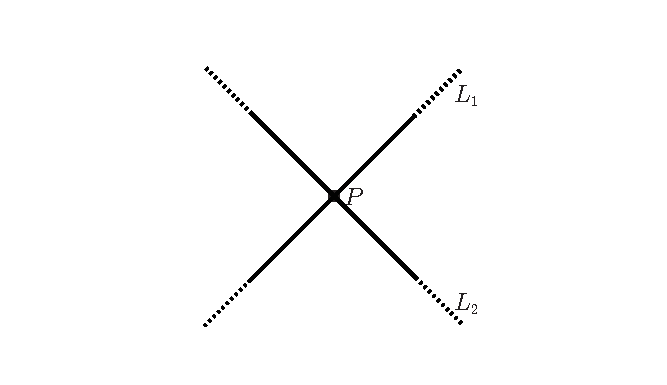
\includegraphics[trim=0cm 0cm 0cm 0cm,clip,scale=0.50]{images/planecurve4.pdf}
	\end{minipage}
\begin{itemize}
	\item $(1,1)$: $C=L_1\cup L_2$ e $P=L_1\cap L_2$.
	\item $(2,0)/(0,2)$: La forma quadratica si fattorizza su $\complexset$ e non su $\realset$; $C$ ha come sostegno un \textit{unico} punto $P$, che è proprio il punto singolare.
\end{itemize}
\end{observe}
\begin{observe}\textsc{Punti singolari e cubiche.}\\
	Nel piano proiettivo $\proj[2]{\kamp}$ consideriamo $C$ una \textit{cubica} di equazione $F=0$ con $\deg F=3$. Se la curva $C$ è \textit{riducibile}, allora il polinomio $F$ è \textit{riducibile} per definizione, ma siccome il grado è solo 3, allora è necessariamente il prodotto di un polinomio di grado 1 per un altro polinomio di grado 2:
	\begin{equation*}
		F=G\cdot H\text{ con }\deg G=1\text{ e }\deg H=2
	\end{equation*}
	Il luogo degli zeri di $F$ è \textit{unione} dei luoghi degli zeri di $G$ e $H$, dunque $C$ è unione di una retta e di una conica.\\ \hspace{-1mm}
	\begin{minipage}{0.75\textwidth}
	\vspace{2mm}
	Supponiamo invece che $C$ sia \textit{irriducibile}: $C$ \textit{non} può contenere una retta, altrimenti l'equazione della retta \textit{dividerebbe} il polinomio $F$. Allora $C$ ha \textit{al più un punto singolare}.
	Supponiamo per assurdo ne abbia almeno due, come $P$ e $Q$: potremmo considerare la retta $r=\overline{PQ}$ che passa per $P$ e $Q$ e intersecarla con la curva. Sicuramente $C\cap r\supseteq \{P,Q\}$ e, siccome $P$ e $Q$ sono due punti singolari, allora la molteplicità di intersezione è almeno 2.
	\end{minipage}
	\hspace{-12mm}
	\begin{minipage}{0.24\textwidth}
		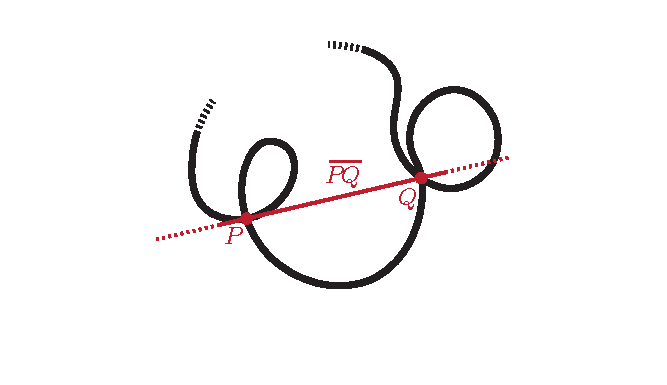
\includegraphics[trim=0cm 0cm 0cm 0cm,clip,scale=0.50]{images/planecurve5.pdf}
	\end{minipage}\\
	Ma ciò non è possibile perché, dallo studio delle intersezioni fra una retta e una curva, sappiamo che dobbiamo contare con molteplicità \textit{fino al grado della curva}: qui ci sono $2$ punti con molteplicità $2$, ma $C$ ha grado 3, dunque la retta dovrebbe essere contenuta nella curva, il che è una contraddizione!
\end{observe}
\begin{example}
	Sia $F=x_0^3+x_1^3+x_2^3$. Essa dà una curva \textit{senza punti singolari} perché le derivate parziali sono multipli delle coordinate, dunque non possono mai essere tutti nulli
\end{example}
		\section{Fasci di coniche proiettive}
		\begin{define}\textsc{Fascio di coniche.}\\
			Siano $C_1$ e $C_2$ due coniche \textit{distinte} nel piano proiettivo $\proj[2]{\ }$ di equazioni $F_1$ e $F_2$, dunque con $F_1$ e $F_2$ sono proporzionali. Il \textbf{fascio di coniche}\index{fascio!di coniche} $\mathcal{F}$ generato da $C_1$ e da $C_2$ è dato da tutte le coniche di equazione:
			\begin{equation}
				C_{\lambda,\mu}\colon \lambda F_1+\mu F_2=0\text{ con }(\lambda\colon \mu)\in \proj[1]{\ }
			\end{equation}
		\vspace{-6mm}
		\end{define}
Notiamo che se moltiplichiamo $\lambda$ e $\mu$ per lo stesso scalare tutta l'equazione viene moltiplicata per lo stesso scalare, riottenendo la stessa conica di prima; $\lambda$ e $\mu$ vanno presi in $\proj[1]{\ }$ e non solo in $\kamp$.
\begin{examples}
	\begin{enumerate}
		\item	Siano $C_1\colon x_0x_1=0$ e $C_2\colon (x_0-x_1)x_2=0$ due coniche, entrambe coppie di rette. Il fascio da loro generato è $C_{\lambda,\mu}\colon \lambda x_0x_1 + \mu (x_0-x_1)x_2=\lambda x_0x_1 + \mu x_0x_2 -\mu x_1x_2=0$.
		\item	Siano $C_1\colon x_0x_1=0$ e $\widetilde{C_2}\colon x_0x_2=0$ due coniche. Il fascio da loro generato è $C_{\lambda,\mu}\colon \lambda x_0x_1 +\mu x_0x_2=x_0(\lambda x_1 + \mu x_2)=0$; siccome $x_0=0$ appartiene ad entrambe le coniche si può raccogliere.
	\end{enumerate}
\vspace{-3mm}
\end{examples}
Dato un fascio di coniche ci si chiede qual è il rango delle coniche del fascio.
\begin{define}\textsc{Conica degenere.}\\ 
Una conica $C$ in $\proj[2]{\ }$ si dice \textbf{degenere}\index{conica!degenere} quando \textit{non} ha rango massimo, ovvero se $\rk C< 3$, dunque quando la matrice non è invertibile.
\end{define}
\begin{digression}
	 Si può dimostrare che il rango della conica,  ‘‘essere riducibili'' e ‘‘essere degeneri'' sono tutte proprietà proiettive. Dalla classificazione delle coniche proiettive (reali o complesse) si vede dunque che una conica è \textit{degenere} se e solo se è \textit{riducibile}.
\end{digression}
\subsection{Studio delle coniche degeneri di un fascio}
Dato un fascio, vogliamo vedere quante e quali sono le coniche degeneri del fascio. Supponiamo che $C_1$ abbia matrice simmetrica associata $A_1$ e $C_2$ abbiamo analogamente $A_2$. È chiaro che la conica del fascio $C_{\lambda,\mu}$ generata da $C_1,\ C_2$ sarà associata alla combinazione lineare $\lambda A_1+\mu A_2$ delle matrici: essa è una matrice $3\times 3$ i cui elementi sono o $0$ o forme lineari in $\lambda$ e $\mu$.\\
Definiamo $D(\lambda,\mu)\coloneqq \det (\lambda A_1+\mu A_2)$, polinomio omogeneo in $\lambda$ e $\mu$. Si hanno due possibilità:
	\begin{itemize}
		\item	$D(\lambda,\ \mu)\equiv 0\implies$ \textit{tutte} le coniche del fascio sono degeneri.
		\item	$D(\lambda,\ \mu)$ è omogeneo di grado 3, dunque le	coniche degeneri corrispondono agli \textit{zeri} del polinomio $D$ su $\proj[1]{\ }$. Poiché essi sono al più 3, ci sono \textit{al più 3 coniche degeneri}.
	\end{itemize}
\begin{tips}
	O tutte le coniche del fascio sono degeneri o sono al massimo 3, quindi se in un fascio ne trovo \textit{quattro} degeneri, allora tutte lo sono!
\end{tips}
Nel \textit{caso complesso} gli zeri (contati con molteplicità) sono pari al grado, dunque si ha sempre almeno una conica degenere. Lo stesso vale anche nel caso reale, essendo il grado del polinomio dispari.
Ristudiamo con quest'ottica gli esempi precedenti.
\begin{examples}
	\begin{enumerate}
		\item	Il fascio è $\mathcal{F}_1\colon 2(\lambda x_0x_1 +\mu x_0x_2 -\mu x_1x_2)=0$ ed ha matrice $A_{\lambda,\mu}=\begin{pmatrix}
			0 & \lambda & \mu \\
			\lambda & 0 & -\mu \\
			\mu & -\mu & 0
		\end{pmatrix}$. Pertanto $D(\lambda,\mu)=\det A_{\lambda,\mu}=-\lambda(\mu^2)+\mu(-\lambda \mu)=-2\lambda\mu^2$. Ci sono solo due zeri di cui uno doppio: $(\lambda\colon\mu)=(1\colon 0)$ oppure $(0\colon 1)$. Questi valori dei parametri ci restituiscono i polinomi di partenza, corrispondono dunque a $C_1$ e $C_2$, che sapevamo già essere degeneri in quanto coppie di rette. Abbiamo dunque scoperto che $C_1$ e $C_2$ sono le \textit{uniche coniche degeneri} del fascio.
		\item	Il fascio è $\mathcal{F}_2 \colon x_0(\lambda x_1+\mu x_2)=0$. In questo caso il determinante viene identicamente nullo $\left(D\equiv 0\right)$. In questo fascio tutte le coniche hanno una retta in comune.
	\end{enumerate}
\end{examples}

\begin{define} \textsc{Punti Base di un fascio di coniche.}\\
	I \textbf{punti base}\index{punti!base} di un fascio di coniche sono i punti che appartengono a \textit{tutte} le coniche del fascio:
		\begin{equation}
			\{\text{punti base}\}=\inter_{C\in\mathcal{F}} C \subset \proj[2]{\ }
		\end{equation}
	\vspace{-3mm}
\end{define}
\begin{observe}	I punti base di un fascio sono dati dall'intersezione delle due coniche che generano il fascio, cioè $C_1\cap C_2$. Infatti, $\displaystyle C_1\cap C_2 \supseteq \inter_{C\in\mathcal{F}} C$. Viceversa se $P\in C_1\cap C_2$ allora:
	\begin{equation*}
		F_1\left(P\right)=0\text{ e }F_2\left(P\right)=0 \implies (\lambda F_1 +\mu F_2)\left(P\right)=0,\ \forall\lambda,\mu \implies P\in C_{\lambda,\mu},\ \forall (\lambda\colon\mu)\in\proj[1]{\ }
	\end{equation*}
Dunque, per ogni qualunque combinazione lineare presa in $P$ si annulla, dunque $P$ è punto comune a tutte le coniche del fascio, cioè un punto base.
\end{observe}
Vediamo i punti base degli esempi precedenti.
\begin{examples}
	\begin{enumerate}
		\item	Per ottenere i punti base del fascio si intersecano le coniche che lo generano:
			\begin{gather*}
				\begin{cases}
					x_0x_1=0\\
					(x_0-x_1)x_2=0
				\end{cases} \implies \begin{cases}
					x_0=x_1=0\\
					x_0=x_2=0\\
					x_1=x_2=0
				\end{cases}
			\end{gather*}
		Intersecando due rette \textit{non} coincidenti si possono ottenere al più 4 punti, ma se ne ottengono meno se qualcuno di questi punti coincide con altri. In questo caso si hanno 3 punti base: $(1\colon 0\colon 0),(0\colon 1\colon 0), (0\colon 0\colon 1)$.
		\item	I punti base sono dati dal sistema:
		\begin{equation*}
			\begin{cases} x_0x_1=0\\ x_0x_2=0 \end{cases}
		\end{equation*}
		$x_0=0$ è una retta appartenente a \textit{tutte} le coniche del fascio, dunque si ha una \textit{retta di punti base}. L'altro punto base è $P=(1\colon 0\colon 0)$; notiamo che quest'ultimo è il punto base del fascio di rette $\lambda x_1+\mu x_2=0$, cioè il fascio di rette che contengono $P$.
	\end{enumerate}
\end{examples}
\begin{digression} \textsc{Nodi e Cuspidi}\\
	Un \textbf{nodo}\index{nodo} è un punto $P$ per cui la retta ‘‘generale'' per $P$ ha intersezione $2$ con la curva e ce ne sono \textit{esattamente} $2$ che hanno intersezione $>2$.\\
	Una \textbf{cuspide}\index{cuspide} è un punto $P$ in cui la retta ‘‘generale'' per $P$ ha intersezione $2$ con la curva e ce n'è \textit{una sola} che ha intersezione $>2$
\end{digression}
%LEZ 36
	\subsection{Parametrizzazione delle coniche nel piano proiettivo}
Data l'equazione generale di una conica $F=a_{00}x_0^2+2a_{01}x_0x_1+\dots+a_{22}x_2^2$ possiamo associare a $C$ il punto $(a_{00}\colon a_{01}\colon a_{02}\colon a_{11}\colon a_{12}\colon a_{22})\in\proj[5]{\ }$, in quanto servono sei coordinate per descrivere una conica. Tale punto la determina univocamente: entrambi sono \textit{non} nulli e determinati \textit{a meno di multipli}.\\
In questo modo otteniamo una \textit{corrispondenza biunivoca} fra le coniche in $\proj[2]{\ }$ e $\proj[5]{\ }$:
	% https://q.uiver.app/?q=WzAsMixbMCwwLCJcXHtcXHRleHR7Y29uaWNoZSBpbiB9XFxwcm9qWzJde1xcIH0gXFx9Il0sWzIsMCwiXFxwcm9qWzVde1xcIH0iXSxbMCwxLCIxXFxjb2xvbiAxIiwwLHsic3R5bGUiOnsidGFpbCI6eyJuYW1lIjoiYXJyb3doZWFkIn19fV1d
	\[\begin{tikzcd}
		{\{\text{coniche in }\proj[2]{\ } \}} && {\proj[5]{\ }}
		\arrow["{1\colon 1}", from=1-1, to=1-3, tail reversed]
	\end{tikzcd}\]
Con questa interpretazione, cosa corrisponde un fascio di coniche?\\
Date $C_1$ e $C_2$ coniche, consideriamo il fascio $\mathcal{F}$ da loro generato: a $C_1\colon F=\sum_{i,j}a_{ij}x_ix_j$ corrisponde ad un punto $A=(a_{00}\colon \cdots \colon a_{22})\in\proj[5]{\ }$ e a $C_2\colon G=\sum_{i,j}b_{ij}x_ix_j$ corrisponde un punto $B=(b_{00}\colon\cdots\colon b_{22})\in\proj[5]{\ }$. La conica $C_{\lambda,\mu}$ del fascio è la combinazione lineare di $F$ e $G$, dunque i coefficienti dei monomi sono la combinazione lineare dei coefficienti delle equazioni di $C_1$ e $C_2$:
	\begin{gather*}
		c_{\lambda,\mu}\colon \lambda F+\mu G=\sum_{i,j}(\lambda a_{ij}+\mu b_{ij})x_ix_j \longleftrightarrow P_{\lambda,\mu} =(\lambda a_{00}+\mu b_{00}\colon \cdots \colon \lambda a_{22}+\mu b_{22})\in\proj[5]{\ }
	\end{gather*}
A $C_{\lambda,\mu}$ associamo il punto $P_{\lambda,\mu}$, le cui coordinate omogenee sono combinazioni lineari di $A$ e $B$. Facendo variare $\lambda$ e $\mu$, il punto $P_{\lambda,\mu}$ descrive in $\proj[5]{\ }$ una retta $\overline{AB}$ generata dai punti $A$ e $B$, pertanto \textit{un fascio di coniche corrisponde esattamente ad una retta in} $\proj[5]{\ }$. Siccome una retta è individuata da due qualsiasi suoi punti, allo stesso modo il fascio è descritto da qualsiasi sue due coniche, pertanto la scelta delle coniche dà solo una \textit{parametrizzazione diversa} del fascio.\\
Questo ci permette di dare alcune informazioni aggiuntive sui punti base:
\begin{tips} \textsc{Calcolo dei punti base con due coniche qualsiasi}.\\
	Dato un fascio $\mathcal{F}$ di coniche, i punti base del fascio sono dati dall'intersezione di \textit{due qualsiasi coniche} del fascio purché siano \textit{distinte}, ovvero da $C\cap\widetilde{C}$ dove $C$ e $\widetilde{C}$ sono due coniche distinte del fascio.
\end{tips}
%così è molto più facile intersecare coppie di rette
\begin{observe}
	Sia $\mathcal{F}$ un fascio di coniche. Esiste \textit{sempre} una conica $C$ degenere in $\mathcal{F}$, quindi usiamo $C$ per calcolare i punti base.\\
	Siccome è degenere, $C$ è l'unione di due rette linearmente indipendenti: $C=l_1\cup l_2$. Scegliamo una qualsiasi altra conica $\widetilde{C}$ del fascio; i punti base del fascio sono dati da $C\cap\widetilde{C}=(l_1\cap\widetilde{C})\cup (l_2\cap \widetilde{C})$.\\
	Ne deduciamo che il numero di punti base di un fascio di coniche, se sono finiti, sono 4: infatti, ciascuna delle due rette interseca $\widetilde{C}$ al più in 2 punti.
\end{observe}

\begin{corollary}
	Se due coniche $C_1$ e $C_2$ non hanno una retta in comune allora:
	\begin{equation}
		\#(C_1\cap C_2)\leq 4
	\end{equation}
\vspace{-6mm}
\end{corollary}
\begin{demonstration}
	$C_1\cap C_2$ sono i punti base del fascio generato da $C_1$ e $C_2$. La tesi segue dall'osservazione precedente.
\end{demonstration}

\begin{tips} \textsc{Calcolo dell'intersezione delle coniche}.\\
	Abbiamo così anche un metodo per calcolare $C_1\cap C_2$ dato il fascio $\mathcal{F}$. Scriviamo $D(\lambda,\ \mu)$, troviamo una conica degenere $\widetilde{C}$ e poi intersechiamo con $C_1\cap\widetilde{C}$. Questo metodo è particolarmente utile nel caso avessimo a che fare con \textit{coniche irriducibili}.
\end{tips}
Ci sono diversi tipi di \textit{rappresentazione geometrica} dei fasci di coniche proiettive; vediamo quello più comune.
\begin{proposition}
	Siano $A,\ B,\ C,\ D$ quattro punti in posizione generale in $\proj[2]{\ }$.\\
	\begin{minipage}{0.75\textwidth}
	La famiglia delle coniche passanti per i quattro punti è un fascio $\mathcal{F}$ avente come punti base esattamente i quattro punti; geometricamente stiamo fissando $A,\ B,\ C,\ D$ e considerando le coniche che passano per tutti e quattro.\\
	Inoltre $\mathcal{F}$ non contiene rette doppie e contiene esattamente 3 coniche degeneri: esse sono le coppie di rette che
	passano per questi 4 punti: $\overline{AB}\cup\overline{CD}$, $\overline{AC}\cup \overline{BD}$, $\overline{AD}\cup\overline{BC}$.
	\end{minipage}
	\hspace{1mm}
	\begin{minipage}{0.24\textwidth}
		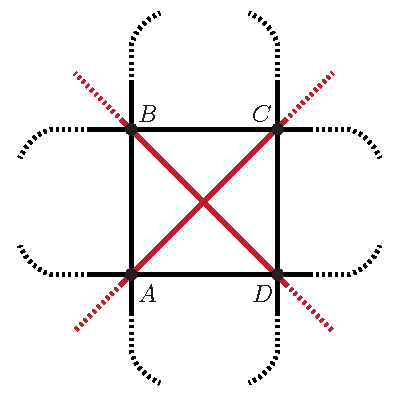
\includegraphics[trim=0cm 0cm 0cm 0cm,clip,scale=0.50]{images/conicfamily.pdf}
	\end{minipage}

%\footnote{il disegno è fuorviante perché le rette si intersecano da qualche parte nel piano proiettivo}
	
%famiglia fascio F: se la consider ocome punti di P5 descrivono esataente una retta: fissate due coniche le altre sono date da cl delle altre 2
%essere un fascio: in P5 è una retta: se guardo le eq tutte e sole che si ottengono come cl di due eq fissate/
%/è un fascio semplice perché il comportamento è quello che uno si aspetta/
\end{proposition}
\begin{demonstration}
	Siccome i 4 punti sono in posizione generale possiamo scegliere delle coordinate in $\proj[2]{\ }$ tali che i primi 3 sono i punti fondamentali e l'ultimo il punto unità: $A=(1\colon0\colon0), B=(0\colon1\colon0),\ C=(0\colon0\colon1),\ D=(1\colon1\colon1)$.\\
	Partiamo dall'equazione di una conica generica e imponiamo che passi per i 4 punti e vediamo le condizioni risultanti sui coefficienti:
		\begin{gather*}
			a_{00}x_0^2+2a_{01}x_0x_1+a_{11}x_1^2+2a_{02}x_0x_2+2a_{12}x_1x_2+a_{22}x_2^2=0\\
			\begin{array}{ll}
				\text{Per } A \colon & a_{00}=0 \\
				\text{Per } B \colon & a_{11}=0 \\
				\text{Per } C \colon & a_{22}=0 \\
				\text{Per } D \colon & 2a_{01}+2a{02}+2a_{12}=0 \implies a_{12}=-a_{01}-a_{02}
			\end{array}\\
			\implies a_{01}x_0x_1+a_{02}x_0x_2-(a_{01}+a_{02})x_1x_2=0
		\end{gather*}
	Abbiamo così le equazioni di tutte e sole le coniche che passano per $A,\ B,\ C,\ D$. Siccome $a_{01}$ e $a_{02}$ sono gli unici parametri rimasti, riscriviamo l'equazione evidenziandoli: $a_{01}x_1(x_0-x_2)+a_{02}x_2(x_0-x_1)=0$. Abbiamo così trovato esattamente un fascio di coniche generato dalle due coniche entrambe degeneri:
		\begin{equation*}
			C_1\colon \underbrace{x_1}_{\overline{AC}} \underbrace{(x_0-x_2)}_{\overline{BD}}=0 \quad
			C_2\colon \underbrace{x_2}_{\overline{AB}} \underbrace{(x_0-x_1)}_{\overline{CD}}=0
		\end{equation*}
	Abbiamo così dimostrato la prima affermazione.\\
	In questo modo abbiamo già trovato due coniche fra quelle degeneri del fascio; possiamo verificare, intersecando le due coniche (e quindi le quattro rette), che i punti base sono solo $A,\ B,\ C,\ D$:
	% Osserviamo ora che i punti base con coordinata $x_1$ zero sono proprio $A$ e $C$, pertanto $x_1=0$ corrisponde alla retta $\overline{AC}$. In modo analogo $x_2=0$ corrisponde alla retta $\overline{AB}$.
		\begin{equation*}
			\begin{array}{ll}
				C_1\cap C_2  & = (\overline{AC}\cup \overline{BD}) \cap (\overline{AB}\cup\overline{CD}) =\\ =(\overline{AC}\cap\overline{AB}) \cup (\overline{AC}\cap\overline{CD}) \cup (\overline{BD}\cap \overline{AB}) \cup (\overline{BD}\cap \overline{CD})=\\ 
				&=\{A,\ B,\ C,\ D\}
			\end{array}
		\end{equation*}
	Avremmo potuto evitare questo conto osservando che sono punti base perché per costruzione tutte le coniche passano per questi 4 punti e, essendo finiti, non possono essercene altri.\\
	Per trovare l'ultima conica degenere scriviamo la matrice associata a meno di multipli alla conica generica del fascio e calcoliamo le radici del suo determinante:
		\begin{gather*}
			M=\begin{pmatrix}
				0 & a_{01} & a_{02} \\
				a_{01} & 0 & -a_{01}-a_{02}\\
				a_{02} & -a_{01}-a{02} & 0
			\end{pmatrix}\\
		\implies D=\det M= -a_{01}a_{02}(a_{01}+a_{02})+a_{02}a_{01}(-a_{01}-a_{02}) = -2a_{01}a_{02}(a_{01}+a_{02})
		\end{gather*}
	È un polinomio omogeneo in $a_{01}$ e $a_{02}$ già fattorizzato in fattori lineari, pertanto si hanno esattamente \textit{tre} coniche degeneri: $a_{01}=0$ dà $C_2$, $a_{02}=0$ dà $C_1$, mentre la terza si ottiene sostituendo nell'equazione del fascio $a_{02}=-a_{01}$, da cui si ha l'equazione $a_{01}x_0x_1-a_{01}x_0x_2=0\implies x_0(x_1-x_2)=0$, corrispondente alle rette $\overline{BC}$ e $\overline{AD}$. Tutte e tre le coniche degeneri hanno rango 2 e quindi \textit{non} ci sono rette doppie nel fascio.
\end{demonstration}

\begin{tips} \textsc{Fascio di coniche per quattro punti in posizione generale}. \label{fascio coniche per 4 pt pos gen} \\
	Se dobbiamo scrivere un fascio $\mathcal{F}$ di coniche per quattro punti procedere come nella dimostrazione può esser lungo; in modo più rapido, scriviamo due delle coniche riducibili con delle rette per i punti:
	\begin{equation*}
		l_1\colon\overline{AB},\ l_2\colon \overline{CD},\ l_3\colon\overline{AC}, l_4\colon \overline{BD} 
	\end{equation*} 
	Le coniche sono $C_1\colon l_1l_2$ e $C_2\colon l_3l_4$; allora l'equazione del fascio è $\mathcal{F}\colon \lambda l_1 l_2 + \mu l_3 l_4 =0$.
\end{tips}
Se un punto di $\proj[2]{\ }$ è un punto base di un fascio, allora appartiene a tutte le coniche di esso. Preso invece un punto \textit{non} base del fascio, quante coniche passano per esso?
\begin{proposition}
	Sia $\mathcal{F}$ un fascio di coniche e sia $P\in \proj[2]{\ }$. Se $P$ \textit{non} è un punto base di $\mathcal{F}$, allora esiste ed è unica la conica del fascio che contiene $P$.
\end{proposition}
\begin{demonstration}
	Supponiamo di avere due coniche $C_1,\ C_2$ che generano il fascio $\mathcal{F}$ con $C_i\colon f_i=0$; il fascio avrà equazione $\mathcal{F}\colon \lambda F_1 +\mu F_2=0$. Il punto $P$ appartiene alla conica generale del fascio se e solo se l'equazione della conica è soddisfatta nel punto:
		\begin{equation*}
			P\in C_{\lambda,\mu} \iff \lambda F_1\left(P\right) +\mu F_2\left(P\right)=0
		\end{equation*}
	Tale equazione può essere vista come un'equazione in $(\lambda \colon \mu)$.\\
	Siccome $P$ non è un punto base, allora \textit{non} appartiene all'\textit{intersezione} delle due coniche, dunque non è possibile che entrambe le equazioni si annullino in P: 
	\begin{equation*}
		P\notin C_1\cap C_2 \implies (F_1\left(P\right), F_2\left(P\right)) \neq \left(0,\ 0\right)
	\end{equation*}
	L'equazione ha un'unica soluzione in $\proj[1]{\ }$ che sarà proprio $(\lambda \colon \mu)=(-F_2\left(P\right)\colon F_1\left(P\right))$, ottenendo così i parametri che descrivono l'unica conica del fascio che contiene $P$.
\end{demonstration}
Dal risultato precedente, possiamo enunciare quando cinque punti determinano una conica proiettiva.
\begin{proposition}
	Dati cinque punti distinti in $\proj[2]{\ }$ \textit{a 4 a 4 non allineati}\footnote{È una condizione più debole rispetto all'essere solo in posizione generale, perché potrebbero essercene tre allineati ma non quattro.}, esiste ed è unica la conica $C$ che li contiene.
\end{proposition}
\begin{demonstration}
	Possiamo sempre scegliere 4 di questi punti in posizione generale.\\
	\begin{minipage}{0.69\textwidth}
	Consideriamo inizialmente $A,\ B,\ C,\ D$:
	\begin{itemize}
	\item Sono in posizione generale: siamo a posto.
	\item Tre sono allineati, per esempio $A,\ B,\ C$.
	\end{itemize}
	Siccome per ipotesi i quattro punti non sono allineati, allora $D\notin r$, $E\notin r$ con $r$ retta per $A,\ B,\ C$.
	\end{minipage}
	%\hspace{-12mm}
	\begin{minipage}{0.3\textwidth}
		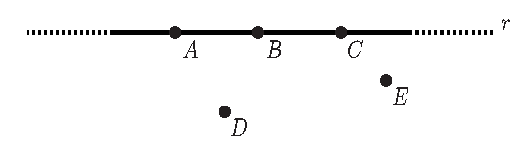
\includegraphics[trim=0cm 0cm 0cm 0cm,clip,scale=0.50]{images/fivepointconic1.pdf}
	\end{minipage}\\
	\begin{minipage}{0.69\textwidth}
	Escludiamo $C$ e consideriamo $A,\ B,\ D,\ E$:
	\begin{itemize}
		\item Sono in posizione generale: siamo a posto.
		\item Tre sono allineati.
	\end{itemize}
	Abbiamo già che $D,E \notin r$, dunque i tre punti allineati possono essere $A,\ D,\ E$ oppure $B,\ D,\ E$. Supponendo siano $A,\ D,\ E$, scartiamo $A$ e otteniamo $B,\ C,\ D,\ E$ in posizione generale.
	\end{minipage}
	%\hspace{-12mm}
	\begin{minipage}{0.30\textwidth}
		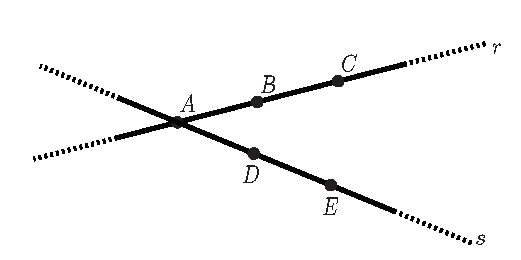
\includegraphics[trim=0cm 0cm 0cm 0cm,clip,scale=0.50]{images/fivepointconic2.pdf}
	\end{minipage}\\
	Possiamo ora applicare la proposizione precedente: sia $\mathcal{F}$ il fascio delle coniche passanti per $A,\ B,\ C,\ D$; poiché $E$ non è un punto base per $\mathcal{F}$ in quanto i punti base sono i cinque punti $A,\ B,\ C,\ D$, esiste ed è \textit{unica} la conica $C$ del fascio che passa per $E$. $C$ è l'unica conica che contiene i cinque punti.
\end{demonstration}
Questa dimostrazione dà anche il metodo per trovare la conica che passa per tali 5 punti.
\begin{tips}
	Per trovare una conica $\mathcal{C}$ che passa per 5 punti dati $A,\ B,\ C,\ D,\ E$ in $\proj[2]{\ }$ potremmo partire dalla conica generale e imporre il passaggio per 5 punti, ma è un calcolo laborioso. Un metodo più rapido è invece il seguente.
		\begin{itemize}
			\item	Scegliere quattro punti in posizione generale $A,\ B,\ C,\ D$.
			\item	Scrivere quattro rette e il fascio $\mathcal{F} $ come nel ‘‘Tips \& Tricks!'' a pag. \pageref{fascio coniche per 4 pt pos gen}.
			\item	Imporre il passaggio per il quinto punto $E$ in modo da trovare la conica $\mathcal{C}$.
		\end{itemize}
	\vspace{-3mm}
\end{tips}
\begin{observe}
	Il passaggio per un punto di una conica generica dà \textit{equazioni lineari omogenee} sui coefficienti della conica; possiamo pensarlo dunque come un \textit{iperpiano} in $\proj[5]{\ }$. È ragionevole aspettarsi che con cinque punti ho cinque iperpiani che, in posizione generale, si intersecano in solo punto.\\
	L'ipotesi sui punti a 4 a 4 non allineati serve a garantire che le condizioni lineari siano \textit{indipendenti}, così da ottenere un punto solo nell'intersezione degli iperpiani.
\end{observe}
\begin{example}~{}\\
		\begin{minipage}{0.69\textwidth}
	Se abbiamo 5 punti di cui 4 allineati su una retta $r$, allora per ogni retta $s$ che passa per $P$ la conica $r\cup s$ contiene i 5 punti, quindi ci sono \textit{infinite coniche} avendo infinite rette $s$.
	\end{minipage}
	%\hspace{-1mm}
	\begin{minipage}{0.3\textwidth}
		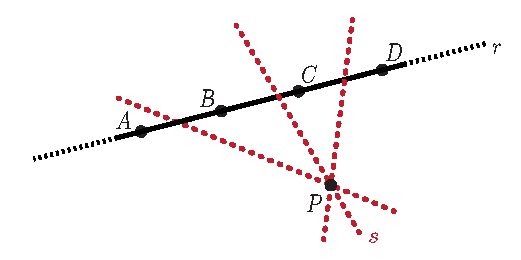
\includegraphics[trim=0cm 0cm 0cm 0cm,clip,scale=0.50]{images/fourpointconic.pdf}
	\end{minipage}
\end{example}
\begin{proposition}~{}\\
	\begin{minipage}{0.72\textwidth}
	Siano 3 punti \textit{non allineati} $A,\ B,\ C\in\proj[2]{\ }$, e sia una retta $r$ che passi per $A$ ma non per $B$ e $C$, ovvero $A\in r$ e $B,\ C\notin r$. La famiglia delle coniche che passano per $A,\ B,\ C$ e sono tangenti a $r$ in $A$ è un fascio $\mathcal{F}$.\\
	I punti base del fascio $\mathcal{F}$ sono solo $A,\ B,\ C$; il fascio \textit{non} contiene rette doppie e ci sono solo due coniche degeneri $\overline{AB}\cup\overline{AC}$ e $r\cup\overline{BC}$.
	\end{minipage}
	\hspace{-2mm}
	\begin{minipage}{0.27\textwidth}
		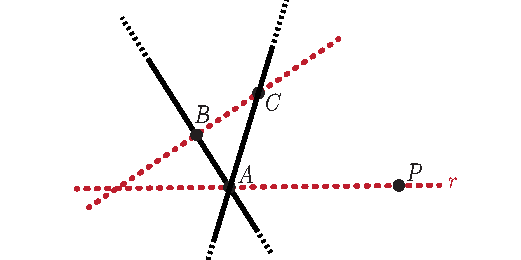
\includegraphics[trim=0cm 0cm 0cm 0cm,clip,scale=0.50]{images/fourpointconic2.pdf}
	\end{minipage}
\end{proposition}
\begin{demonstration}
	Sia $P\in r$ un punto diverso da $A$ e $P\notin\overline{BC}$. $A,\ B,\ C,\ P$ sono in posizione generale, perché a tre a tre non allineati. Scegliamo le coordinate proiettive tali che $A,\ B,\ C$ siano i punti coordinati mentre $P$ il punto unità: $A=(1\colon 0\colon 0),B=(0\colon 1\colon 0),C=(0\colon 0\colon 0\colon1)$.
	Allora la retta $r=\overline{AP}$ ha equazione $x_1-x_2=0$.\\
	Si consideri la conica generale:
	\begin{equation*}
		a_{00}x_0^2+2a_{01}x_0x_1+a_{11}x_1^2+2a_{02}x_0x_2+2a_{12}x_1x_2+a_{22}x_2^2=0
	\end{equation*}
	Sappiamo già che il passaggio per i punti coordinati annulla la diagonale della matrice associata:
	\begin{equation*}
		\begin{array}{ll}
			\text{Per } A \colon & a_{00}=0 \\
			\text{Per } B \colon & a_{11}=0 \\
			\text{Per } C \colon & a_{22}=0 \\
		\end{array}
	\implies F=a_{01}x_0x_1+a_{12}x_1x_2+a_{02}x_0x_2
	\end{equation*}
	Intersechiamo con $r\colon x_1=x_2$ e sostituiamo in $F$:
	\begin{equation*}
		a_{01}x_0x_+a_{12}x_1^2+a_{02}x_0x_1=0\implies x_1((a_{01}+a_{02})x_0+a_{12}x_1)=0
	\end{equation*}
	Notiamo che $x_1=0$ è dovuto al fatto che $A\in r\cap C$. Ne segue che $r$ è tangente alla conica in $A$ se e solo se $A$ ha molteplicità due, quindi se e solo $x_1=0$ è l'unica soluzione. Necessariamente il coefficiente di $x_0$ nell'equazione precedente deve essere nullo, cioè $a_{01}+a_{02}=0\implies a_{02}=-a_{01}$. Sostituendo nell'equazione si ottiene:
		\begin{equation*}
			a_{01}x_0x_1 -a_{01}x_0x_2 + a_{12}x_1x_2=0 \implies a_{01}x_0(x_1-x_2) + a_{12}x_1x_2=0
		\end{equation*}
	Quest'equazione descrive tutte e sole le coniche per $A,\ B,\ C$ e tangenti a $r$ in $A$; in questo modo abbiamo verificato che è un fascio $\mathcal{F}$.\\
	Le coniche che lo generano sono $C_1\colon \underbrace{x_0}_{\overline{BC}} \underbrace{(x_1-x_2)}_{r}$ e $C_2\colon \underbrace{x_1}_{\overline{AC}} \underbrace{x_2}_{\overline{AB}}$. Intersecando $C_1$ e $C_2$ otteniamo i punti base:
		\begin{gather*}
			C_1\cap C_2 = (\overline{BC}\cup r) \cap (\overline{AC}\cup\overline{AB})=(\overline{BC}\cap\overline{AC}) \cup (\overline{BC}\cap\overline{AB}) \cup (r\cap\overline{AC}) \cup (r\cap\overline{AB}) =\{ C,B,A \}
		\end{gather*}
	Scriviamo la matrice per verificare che non ci siano altre coniche degeneri e altri punti base:
		\begin{gather*}
			M=\begin{pmatrix}
				0 & a_{01} & -a_{01}\\
				a_{01} & 0 & a_{12}\\
				-a_{01} & a_{12} & 0
			\end{pmatrix}\\
			D=\det M= -a_{01}(a_{01}a_{12}) -a_{01}(a_{01}a_{12}) = -2a_{01}^2 a_{12}
		\end{gather*}
	Siccome $D$ è un polinomio omogeneo di grado 3 si ha una radice doppia, ma le due radici danno le coniche che generano il fascio e dunque le uniche coniche degeneri sono solo $C_1$ e $C_2$.
	% \footnote{Le due coppie di rette soddisfano le condizioni necessarie: nella prima si intersecano in $A$ e la molteplicità di intersezione è 2, conta 1 per ciascuna retta, pertanto la retta è tangente, dal punto di vista dei punti singolari invece la retta è singolare, e ogni retta per $A$ è tangente; mentre la seconda coppia passa per $A,\ B,\ C$ e contiene $r$, dunque siccome quando è contenuta è tangente si ha molteplicità infinita.}
\end{demonstration}

\begin{observe}
	Un fascio di questo tipo è il primo esempio a pag. \pageref{esempi lez 35}.\\
	\begin{minipage}{0.72\textwidth}
	Consideriamo $C_1\colon x_0x_1=0$ e $C_2\colon (x_0-x_1)x_2=0$. Allora, la retta $x_0-x_1=0$ passa per il punto di intersezione delle prime due rette $x_0=0$ e $X_1=0$, quindi siamo nella situazione precedente: $A$ è il punto di intersezione, mentre $B$ e $C$ sono i punti di intersezione di $x_2=0$ con $x_0=0$ e $x_1=0$. Dunque $C_2$ diventa $r\cup \overline{BC}$, mentre $C_1$ è $\overline{AB}\cup \overline{AC}$.
	\end{minipage}
	\hspace{-5mm}
	\begin{minipage}{0.27\textwidth}
		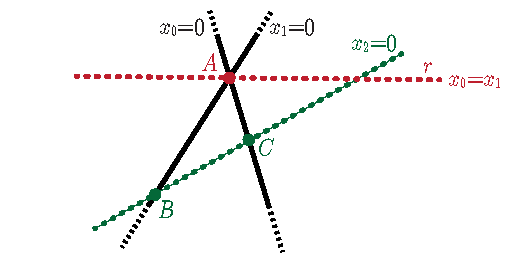
\includegraphics[trim=0cm 0cm 0cm 0cm,clip,scale=0.50]{images/fourpointconic3.pdf}
	\end{minipage}\\
Abbiamo già verificato che i punti base sono solo $A,\ B,\ C$ e che $C_1$ e $C_2$ sono le uniche coniche degeneri di $\mathcal{F}$ ed ora osserviamo che la retta $r$ è tangente a tutte le coniche del fascio.
\end{observe}
%DISEGNO
\subsection{Impratichiamoci! Fasci di coniche proiettive}
\begin{exercise} \textsc{F.F.P., 2.1.}\\
	Nel piano proiettivo reale $\proj[2]{\realset}$ consideriamo i punti:
	\begin{equation*}
		A=(0\colon 1 \colon 2),\ B=(0\colon 0\colon 1),\ C=(2\colon1\colon2),\ D=(3\colon0\colon1)
	\end{equation*}
	Determinare, se esiste, l'equazione di una conica passante per $A,\ B,\ C,\ D$ e tangente in $C$ alla retta $r$ di equazione $x_0-x_2=0$ che passa per $C$.
\end{exercise}
\begin{solution}
	Controlliamo che i 4 punti siano in posizione generale verificando,  con i determinanti, che siano a 3 a 3 non allineati:
		\begin{equation*}
			\begin{array}{ll}
				\begin{vmatrix}
					0 & 0 & 2\\
					1 & 0 & 1\\
					2 & 1 & 2
				\end{vmatrix} \neq 0 \implies A,\ B,\ C \text{ non allineati} & 
				\quad\begin{vmatrix}
					0 & 0 & 3\\
					1 & 0 & 0\\
					2 & 1 & 1
				\end{vmatrix} \neq 0 \implies A,\ B,\ D \text{ non allineati} \\
			\begin{vmatrix}
				0 & 2 & 3\\
				0 & 1 & 0\\
				1 & 2 & 1
			\end{vmatrix} \neq 0 \implies B,\ C,\ D \text{ non allineati} &
			\quad \begin{vmatrix}
				0 & 2 & 3\\
				1 & 1 & 0\\
				2 & 2 & 1
			\end{vmatrix} \neq 0 \implies A,\ C,\ D \text{ non allineati}
			\end{array}
		\end{equation*}
	Dunque c'è un fascio $\mathcal{F}$ di coniche per $A,\ B,\ C,\ D$. Scriviamo l'equazione delle quattro rette con il determinante formale delle coordinate:
		\begin{gather*}
			\begin{array}{lll}
			\text{Retta } \overline{AB} \colon & \begin{vmatrix}
					x_0 & x_1 & x_2 \\
					0 & 1 & 2 \\
					0 & 0 & 1 
				\end{vmatrix} & = x_0=0\\
			\text{Retta } \overline{CD} \colon & \begin{vmatrix}
				x_0 & x_1 & x_2 \\
				2 & 1 & 2 \\
				3 & 0 & 1 
			\end{vmatrix} & = x_0- x_1 (-4) + x_2(-3)=x_0 +4x_1-3x_2=0\\
			&& \implies C_1\colon x_0(x_0+4x_1-3x_2)\\
			\text{Retta } \overline{BD} \colon & \begin{vmatrix}
					x_0 & x_1 & x_2 \\
					0 & 0 & 1 \\
					3 & 0 & 1 
				\end{vmatrix} & = x_1=0\\
				\text{Retta } \overline{AC} \colon & \begin{vmatrix}
					x_0 & x_1 & x_2 \\
					0 & 1 & 2 \\
					2 & 1 & 2 
				\end{vmatrix} & = -x_1(-4) +x_2(-2)= 4x_1 -2x_2=0 \implies 2x_1-x_2=0\\
			&& \implies C_2 \colon x_1(2x_1-x_2) \\
			\end{array}\\
			\text{fascio } \mathcal{F}\colon \lambda x_0(x_0+4x_1-3x_2) +\mu x_1(2x_1-x_2)=0
		\end{gather*}
	Queste sono tutte e sole le coniche che passano per $A,\ D$. Vogliamo la conica del fascio che è tangente alla retta $r\colon x_0-x_2=0$ in $C$. Intersechiamo la conica $C_{\lambda,\mu}$ con la retta $r$ sostituendo $x_2=x_0$ nell'equazione:
		\begin{equation*}
			\begin{array}{lll}
				\lambda x_0(x_0+4x_1-3x_0)+\mu x_1(2x_1-x_0)=0 & \implies & \lambda x_0(4x_1-2x_0)+ \mu x_1(2x_1-x_0)=0\\
				\implies 2\lambda x_0(2x_1-x_0)+ \mu x_1(2x_1-x_0)=0 & \implies & (2x_1-x_0)(2\lambda x_0 +\mu x_1)=0
			\end{array}
		\end{equation*}
	Sostituendo $x_2=x_0$ stiamo parametrizzando la retta $r$ come $(x_0\colon x_1\colon x_0)$. Il passaggio per $C=(2\colon1\colon2)$ corrisponde al primo fattore $x_0=2x_1$. Pertanto, la retta $r$ è tangente alla conica nel punto $C$ se e solo se anche l'altra soluzione corrisponde al punto $C$, cioè se e solo se $2\lambda x_0 +\mu x_1$ e $-x_0+2x_1$ sono proporzionali:
	\begin{equation*}
		\det \begin{pmatrix} 
			2\lambda & \mu \\
			-1 & 2
		\end{pmatrix} =0 \iff 4\lambda +\mu=0 \implies \mu=-4\lambda
	\end{equation*}
	Ad esempio, per $\lambda=1$ e $\mu=-4$ si ha $2\lambda x_0+\mu x_1=2x_0-4x_1$. L'equazione della conica sarà $\mathcal{C} \colon x_0(x_0+4x_1-3x_2) -4x_1(2x_1-x_2)=0 \implies \mathcal{C}\colon x_0^2 +4x_0x_1 -3x_0x_2 -8x_1^2 +4x_1x_2=0$, dunque esiste ed è unica la conica cercata.\\
	Controlliamo se la conica fa quello che deve fare. Passa per i punti dati? Sì, infatti:
	\begin{equation*}
		\begin{array}{ll}
			F(A)=F(0,1,2)=-8+8=0 & F(B)=F(0,0,1)=0 \\
			F(C)=F(2,1,2)= 4+8-12-8+8 =0 & F(D)=F(3,0,1)=9-9=0
		\end{array}
	\end{equation*}
	È tangente a $r$ in $C$? Scriviamo direttamente la tangente alla conica nel punto $C=(2\colon1\colon2)$ con le derivate parziali:
		\begin{gather*}
			\begin{array}{lll}
				\frac{\partial{F}}{\partial{x_0}} = 2x_0+4x_1-3x_2 & \frac{\partial{F}}{\partial{x_1}} = 4x_0-16 x_1 +4x_2 & \frac{\partial{F}}{\partial{x_2}} = -3x_0 +ax_1\\
				\frac{\partial{F}}{\partial{x_0}} (2,1,2) =4+4-6=2 & \frac{\partial{F}}{\partial{x_1}} (2,1,2) =8-16+6=0 & \frac{\partial{F}}{\partial{x_2}} (2,1,2) = -6+4=2\\
			\end{array}\\
			\implies 2x_0-2x_2=0 \implies x_0-x_2=0
		\end{gather*}
	Otteniamo proprio la retta $r$.
\end{solution}
%\part{Geometria proiettiva}
%\labelPart{fourth}
%\include{chapters/chap14}
%\include{chapters/chap15}
%\include{chapters/chap16}
%\include{chapters/chap17}
%\include{chapters/chap18}
%\appendix
\part{Appendici}
\labelPart{appendici}
% SVN info for this file
\svnidlong
{$HeadURL$}
{$LastChangedDate$}
{$LastChangedRevision$}
{$LastChangedBy$}

\chapter{Note aggiuntive}
\labelAppendix{footnotes}
\addtocontents{define}{\noindent\textls{\textsc{\textcolor{reddo}{Appendice A:}
\nowtitle}}
}{}
\addtocontents{theorema}{\noindent\textls{\textsc{\textcolor{reddo}{Appendice A:}
			\nowtitle}}
}{}
\begin{introduction}
‘‘Le note a piè di pagina sono le superfici ingannatrici che permettono ai paragrafi tentacolari di aderire alla realtà più ampia della biblioteca.''
\begin{flushright}
	\textsc{Nicholson Baker,} bibliotecario di Cthulhu.
\end{flushright}
\end{introduction}

\noindent Riportiamo alcune note, precisazioni e dimostrazioni complementari agli argomenti dei capitoli principali che possono risultare utili al lettore
\section{Capitolo 1: spazi topologici}
\subsection{Alcune proprietà della continuità}
Le seguenti dimostrazioni sulle continuità di funzioni sono da \cite{munkres:2000topology}.
\begin{theorema}[Inclusione è funzione continua; Munkres, 18.2b.]~{}\\
	Se $Z\subseteq X$ è sottospazio, l'inclusione $\incl{i}{Z}{X}$ è una funzione continua.
\end{theorema}
\begin{demonstration}
	Se $A$ è un aperto in $X$, allora $i^{-1}\left(A\right)=A\cap Z$ è un aperto in $Z$ per definizione della topologia di sottospazio.
\end{demonstration}
\begin{theorema}[Restrizione di una funzione continua è continua; Munkres, 18.2d.]~{}\\
	Se $\funz{f}{X}{Y}$ è una funzione continua, allora $\funz{f_{\mid Z}}{Z}{Y}$ è continua per ogni sottospazio $Z\subseteq X$.
\end{theorema}
\begin{demonstration}
	La funzione $f_{\mid Z}$ è la composizione dell'inclusione $\incl{i}{Z}{X}$ con la funzione $\funz{f}{X}{Y}$. Poiché la composizione di funzioni continue è continua (teorema \ref{compfunzcont}, pag. \pageref{compfunzcont}), segue la tesi.
\end{demonstration}
La seguente dimostrazione sulle restrizioni di omeomorfismi è un'elaborazione personale sulla base dei teoremi precedenti.
\begin{corollary}[Restrizione di un omeomorfismo è omeomorfismo.]~{}\\
Se $\funz{f}{X}{Y}$ è un omeomorfismo, allora $\funz{f_{\mid Z}}{Z}{f\left(Z\right)}$ è omeomorfismo per ogni sottospazio $Z\subseteq X$. In particolare, $\funz{f_{X\setminus Z}}{X\setminus Z}{Y\setminus f\left(Z\right)}$.
\end{corollary}
\begin{demonstration}
	La restrizione di una funzione è sempre una biezione e, per il teorema precedente, è anche continua. Ciò vale sia per $f$, sia per l'inversa $f^{-1}$ e segue dunque la prima tesi. La seconda parte del corollario vale perché, se $f$ è biettiva, allora:
	\begin{equation*}
		f\left(X\setminus Z\right)=f\left(X\right)\setminus f\left(Z\right)=Y\setminus f\left(Z\right)
	\end{equation*}
\vspace{-3mm}
\end{demonstration}
\begin{attention}
	Non vale il viceversa del teorema precedente: \textit{non è vero} che se $A,\ B\subseteq X$ sono omeomorfi, allora $X\setminus A$ e $X\setminus B$ sono omeomorfi!\\
	Preso ad esempio $A=S^2\setminus\left\{(0,\ 0,\ 1),\ (0,\ 0,\ -1)\right\}$ e $B=S^1\times \realset$. Si ha che $A$ e $B$ sono \textit{omeomorfi} (per proiezione dall'origine), ma $\realset^3\setminus A$ è connesso per archi, mentre $\realset^3\setminus B$ non è \textit{neppure connesso}.
\end{attention}
\subsection{Strutture topologiche e unione/intersezione insiemistica}
La seguente dimostrazione è adattata da \cite{shalop:interior} su Mathematics Stack Exchange.
\begin{lemming}[Interno come complementare della chiusura del complementare.]~{}\\
Sia $A\subseteq X$ con $X$ spazio topologico. Allora:
\begin{equation}
	\interior{A}=X\setminus\left(\overline{X\setminus A}\right)
\end{equation}
\vspace{-6mm}
\end{lemming}
\begin{demonstration}~{}\\
$\includedx$ Dato che $X\setminus A\subseteq \overline{X\setminus A}$, segue che $X\setminus \left(\overline{X\setminus A}\right)\subseteq A$. Allora $X\setminus \left(\overline{X\setminus A}\right)$ è un aperto (perché complementare di un chiuso) contenuto in $A$, pertanto $X\setminus \left(\overline{X\setminus A}\right)\subseteq \interior A$.\\
$\includesx$ Sappiamo che $\interior{A}\subseteq A$, dunque $X\setminus A\subseteq X\setminus \interior A$. Allora $X\setminus \interior A$ è un chiuso (perché complementare di un aperto) contenente $X\setminus A$, pertanto $\overline{X\setminus A}\subseteq X\setminus \interior{A}$, da cui $\interior{A}\subseteq X\setminus\left(\overline{X\setminus A}\right)$.
\end{demonstration}
\begin{proposition}[Strutture topologiche e unione/intersezione insiemistica.]~{}\\\label{chiusurainterno}
Siano $\{A_i\}_{i\in I}$ una famiglia di sottoinsiemi di uno spazio topologico $X$. Allora:
\begin{enumerate}
	\item La chiusura dell'unione degli $A_i$ contiene l'unione delle chiusure degli $A_i$; se gli $A_i$ sono \textit{finiti} allora vale anche il viceversa, ma non necessariamente se $\left|I\right|=\infty$.
	\begin{equation}
		\overline{\bigcup_{i\in I}A_i}\supseteq\bigcup_{i\in I}\overline{A_i}\qquad\overline{\bigcup_{i\in I}A_i}=\bigcup_{i\in I}\overline{A_i}\text{ se }I\text{ finito}
	\end{equation}
	\item La chiusura dell'intersezione degli $A_i$ è contenuta nell'intersezione delle chiusure degli $A_i$; il viceversa non vale necessariamente.
		\begin{equation}
		\overline{\bigcap_{i\in I}A_i}\subseteq\bigcap_{i\in I}\overline{A_i}
	\end{equation}
	\item L'interno dell'unione degli $A_i$ contiene l'unione degli interni degli $A_i$; il viceversa non vale necessariamente.
	\begin{equation}
		\interior{\left(\bigcup_{i\in I}A_i\right)}\supseteq\bigcup_{i\in I}\interior{A_i}
	\end{equation}
	\item L'interno dell'intersezione degli $A_i$ è contenuta nell'intersezione degli interni degli $A_i$; se gli $A_i$ sono \textit{finiti} allora vale anche il viceversa, ma non necessariamente se $\left|I\right|=\infty$.
	\begin{equation}
		\interior{\left(\bigcap_{i\in I}A_i\right)}\subseteq\bigcap_{i\in I}\interior{A_i}\qquad\interior{\left(\bigcap_{i\in I}A_i\right)}=\bigcap_{i\in I}\interior{A_i}\text{ se }I\text{ finito}
	\end{equation}
\end{enumerate}
\end{proposition}
\begin{demonstration}~{}
	\begin{enumerate}[label=\Roman*]
	\item Poichè $A_i\subseteq \bigcup_{i\in I}A_i\ \forall i\in I$ e la chiusura mantiene l'ordine di inclusione, allora:
	\begin{equation*}
		\overline{A_i}\subseteq \overline{\bigcup_{i\in I}A_i}\forall i\in I
	\end{equation*}
	L'unione degli $A_i$ è il più piccolo insieme che contiene ogni $\overline{A_i}$, dunque è contenuto necessariamente in $\displaystyle \overline{\bigcup_{i\in I}A_i}$, pertanto vale il caso generale.\\
	Ponendoci nel caso \textit{finito}, dobbiamo mostrare l'altra inclusione, cioè:
	\begin{equation*}
		\overline{\bigcup_{i\in I}A_i}\subseteq\bigcup_{i\in I}\overline{A_i}
	\end{equation*}
	Poichè gli $\overline{A_i}$ sono chiusi, la loro unione finita è ancora chiusa e pertanto:
	\begin{equation*}
		\overline{\bigcup_{i\in I}\overline{A_i}}=\bigcup_{i\in I}\overline{A_i}
	\end{equation*}
	Per definizione $A_i\subseteq\overline{A_i}\ \forall i$, dunque anche le unioni finite mantengono la relazione di inclusione:
	\begin{equation*}
		\bigcup_{i\in I}A_i\subseteq\bigcup_{i\in I}\overline{A_i}
	\end{equation*}
	Il passaggio alla chiusura mantiene le relazioni di inclusione:
	\begin{equation*}
			\overline{\bigcup_{i\in I}A_i}\subseteq\overline{\bigcup_{i\in I}\overline{A_i}}=\bigcup_{i\in I}\overline{A_i}
	\end{equation*}
	Segue così la tesi.\\
	Come controesempio nel caso \textit{infinito}, si consideri $\realset$ con la topologia Euclidea e la famiglia di sottoinsiemi $\left\{A_n\right\}=\left\{\left[\frac{1}{n},\ 1\right]\mid n\geq 2,\ n\in \naturalset\right\}$. Essi sono chiusi, quindi $A_n=\overline{A_n}$. Allora:
	\begin{equation*}
		\bigcup_{n\geq 2}\overline{A_n}=\bigcup_{n\geq 2}A_n=\left(0,\ 1\right]
	\end{equation*}
Tuttavia, $\displaystyle \overline{\bigcup_{n\geq 2}A_n}=\overline{\left(0,\ 1\right]}=\left[0,\ 1\right]\supsetneqq\left(0,\ 1\right]=\bigcup_{n\geq 2}\overline{A_n}$.
\item Poichè gli $\overline{A_i}$ sono chiusi, la loro intersezione arbitraria è ancora chiusa e pertanto:
\begin{equation*}
	\overline{\bigcap_{i\in I}\overline{A_i}}=\bigcap_{i\in I}\overline{A_i}
\end{equation*}
Per definizione $A_i\subseteq\overline{A_i}\ \forall i$, dunque anche le intersezioni mantengono la relazione di inclusione:
\begin{equation*}
	\bigcap_{i\in I}A_i\subseteq\bigcap_{i\in I}\overline{A_i}
\end{equation*}
Essendo la chiusura il più piccolo chiuso contenente un sottospazio, segue che:
\begin{equation*}
	\bigcap_{i\in I}A_i\subseteq\overline{\bigcap_{i\in I}A_i}\subseteq\bigcap_{i\in I}\overline{A_i}
\end{equation*}
Da cui segue la tesi.\\
Come controesempio, si consideri $\realset$ con la topologia Euclidea. Presi i razionali $\rationalset$ e gli irrazionali $\irrationalset$, essi sono \textit{densi} e quindi $\overline{\rationalset}=\realset$, $\overline{\irrationalset}=\realset$. Allora:
\begin{equation*}
	\overline{\rationalset}\cap\overline{\irrationalset}=\realset
\end{equation*}
Tuttavia, $\rationalset$ e $\irrationalset$ sono disgiunti, pertanto:
\begin{equation*}
	\overline{\rationalset\cap\left(\irrationalset\right)}=\overline{\emptyset}=\emptyset
\end{equation*}
Pertanto \textit{non} vale l'altra inclusione.
\item Passiamo al complementare della chiusura del complementare:
\begin{equation*}
\interior{\left(\bigcup_{i\in I}A_i\right)}=X\setminus\left(\overline{X\setminus \bigcup_{i\in I}A_i}\right)=X\setminus\left(\overline{\bigcap_{i\in I}X\setminus A_i}\right)
\end{equation*}
Poiché $\displaystyle \overline{\bigcap_{i\in I}X\setminus A_i}\subseteq \bigcap_{i\in I}\overline{X\setminus A_i}$, allora $\displaystyle X\setminus\left(\overline{\bigcap_{i\in I}X\setminus A_i}\right) \supseteq X\setminus\bigcap_{i\in I}\overline{X\setminus A_i}$. Pertanto:
\begin{equation*}
\interior{\left(\bigcup_{i\in I}A_i\right)}\supseteq X\setminus\bigcap_{i\in I}\overline{X\setminus A_i}=X\setminus\bigcap_{i\in I}X\setminus \interior{A_i}=X\setminus\left(X\setminus\bigcup_{i\in I}A_i \right)=\bigcup_{i\in I}\interior{A_i}
\end{equation*}
Come controesempio, si consideri $\realset$ con la topologia Euclidea e i sottoinsiemi $A_1=\left[0,\ \frac{1}{2}\right]$ e $A_2=\left[\frac{1}{2},\ 1\right]$. Allora:
\begin{equation*}
	\begin{array}{l}
		\interior{\left(A_1\cup A_2\right)}=\interior{\left(\left[0,\ \frac{1}{2}\right]\cup\left[\frac{1}{2},\ 1\right]\right)}=\interior{\left[0,\ 1\right]}=\left(0,\ 1\right)\\
		\interior{A_1}\cup \interior{A_2}=\interior{\left[0,\ \frac{1}{2}\right]}\cup\interior{\left[\frac{1}{2},\ 1\right]}=\interior{\left[0,\ 1\right]}=\left(0,\ \frac{1}{2}\right)\cup\left(\frac{1}{2},\ 1\right)
	\end{array}
\end{equation*}
Dunque $\interior{A_1}\cup \interior{A_2}\subsetneqq\interior{\left(A_1\cup A_2\right)}$.
\item Passiamo al complementare della chiusura del complementare:
\begin{equation*}
\interior{\left(\bigcap_{i\in I}A_i\right)}=X\setminus\left(\overline{X\setminus \bigcap_{i\in I}A_i}\right)=X\setminus\left(\overline{\bigcup_{i\in I}X\setminus A_i}\right)
\end{equation*}
Poiché $\displaystyle \overline{\bigcup_{i\in I}X\setminus A_i}\supseteq \bigcup_{i\in I}\overline{X\setminus A_i}$, allora $\displaystyle X\setminus\left(\overline{\bigcup_{i\in I}X\setminus A_i}\right) \subseteq X\setminus\bigcup_{i\in I}\overline{X\setminus A_i}$. Pertanto:
\begin{equation*}
		\interior{\left(\bigcap_{i\in I}A_i\right)}\stackrel{!}{\subseteq} X\setminus\bigcup_{i\in I}\overline{X\setminus A_i}=X\setminus\bigcup_{i\in I}X\setminus \interior{A_i} =X\setminus\left(X\setminus\bigcap_{i\in I}A_i \right)=\bigcap_{i\in I}\interior{A_i}
\end{equation*}
Ponendoci nel caso \textit{finito}, l'inclusione con (!) risulta un uguaglianza per il punto 1 della proposizione, da cui segue la tesi.\\
Come controesempio nel caso \textit{infinito}, si consideri $\realset$ con la topologia Euclidea e la famiglia di sottoinsiemi $\left\{A_n\right\}=\left\{\left(1-\frac{1}{n},\ 1+\frac{1}{n}\right)\mid n> 0,\ n\in \naturalset\right\}$. Essi sono aperti, quindi $A_n=\interior{A_n}$. Allora:
\begin{equation*}
	\bigcap_{n>0}\interior{A_n}=\bigcap_{n>0}A_n=\{1\}
\end{equation*}
Tuttavia, $\displaystyle \interior{\left(\bigcap_{n>0}A_n\right)}=\interior{\{1\}}=\emptyset$.
\end{enumerate}
	\vspace{-3mm}
\end{demonstration}
\subsection{Strutture topologiche e prodotto cartesiano}
La dimostrazione del terzo punto è adattata da \cite{Math1000:interior} su Mathematics Stack Exchange.
\begin{proposition}[Strutture topologiche e prodotto cartesiano.]~{}\\\label{topologiaprodottostruttura}
	Siano $X,\ Y$ spazi topologici e $X\times Y$ il loro prodotto.
	\begin{enumerate}
		\item Dati $x\in X,\ y\in Y$, siano $\mathcal{U} = \left\{U_i\right\}_{i\in I}$ un
		sistema fondamentale di intorni di $x$ e $\mathcal{V} = \left\{V_j\right\}_{j\in J}$ un sistema fondamentale di intorni di $y$. Poniamo $W_{ij} \coloneqq U_i \times V_j \subseteq X \times Y$ . Allora:
		\begin{equation}
			\mathcal{W} = \left\{W_{ij}\right\}_{j\in J}
		\end{equation}
		è un sistema fondamentale di intorni di $\left(x,\ y\right) \in X \times Y$.
		\item Se $A\subseteq X,\ B\subseteq Y$, allora $\overline{A\times B}=\overline{A}\times \overline{B}$. In particolare, il prodotto di chiusi è chiuso.
		\item Se $A\subseteq X,\ B\subseteq Y$, allora $\interior{\left(A\times B\right)}=\interior{A}\times \interior{B}$. In particolare, il prodotto di aperti è aperti.
	\end{enumerate}
	\vspace{-3mm}
\end{proposition}
\begin{demonstration}~{}
	\begin{enumerate}[label=\Roman*]
		\item Per definizione di sistema fondamentale di intorni si ha:
		\begin{gather*}
			\forall U\in I\left(x\right)\ \exists U_i\in\mathcal{U}\ \colon U_i\in U\\
			\forall V\in I\left(y\right)\ \exists V_i\in\mathcal{V}\ \colon V_j\in V
		\end{gather*}
		$\impliesdx$ Per ogni intorno $U\in I\left(x\right)$ e $V\in I\left(y\right)$, si ha $W\coloneqq U\times V\in I\left(\left(x,\ y\right)\right)$ per definizione di topologia prodotto. Inoltre, presi gli intorni $U_i$ e $V_j$ definiti come sopra, si ha che $W_{ij} = U_i \times V_j\in I\left(\left(x,\ y\right)\right)$ per definizione di topologia prodotto; segue che, per ogni intorno $W$ di questa forma esiste $W_{ij}$ tale che:
		\begin{equation*}
			W_{ij} = U_i \times V_j\subseteq U\times V= W
		\end{equation*}
		$\impliessx$ Prendiamo un intorno $W\in I\left(x,\ y\right)$, esiste un aperto $W'\subseteq W$. Poiché $W'$ appartiene al prodotto $X\times Y$, si ha che $\displaystyle W'=\bigcup_k A_k\times B_k$ con $A_k$ e $B_k$ aperti di $X$ e $Y$. Preso allora $\left(x,\ y\right)\in W'$, esistono degli aperti $A_k$ e $B_k$ che contengono rispettivamente $x$ e $y$.\\
		Segue dunque che $A_k\in I\left(x\right)$ e $B_k\in I\left(y\right)$ e dunque dal sistema fondamentale di intorni si ha che $\exists U_i\in\mathcal{U},\ V_j\in\mathcal{V}$ tali che $U_i\in A_k,\  V_j\in B_k$. Allora definito $W_{ij} \coloneqq U_i \times V_j$, si ha per ogni intorno $W$ di $X\times Y$ esiste $W_{ij}$ tale che:
		\begin{equation*}
			W_{ij} = U_i \times V_j\subseteq A_k\times B_k\subseteq W'\subseteq W
		\end{equation*}
		\item Utilizziamo i risultati del punto 1 con la caratterizzazione per intorni della chiusura.
		\begin{align*}
			\left(x,\ y\right)\in \overline{A\times B}&\iff \forall W\in I\left(x,\ y\right)\quad W\cap\left(A\times B\right)\neq \emptyset\\
			&\iff \forall U\in I\left(x\right),\ \forall V\in I\left(y\right)\quad \left(U\times V\right)\cap\left(A\times B\right)\neq \emptyset\\
			&\iff \forall U\in I\left(x\right),\ \forall V\in I\left(y\right)\quad \left(U\cap A\right)\times\left(V\cap B\right)\neq \emptyset\\
			&\iff \forall U\in I\left(x\right),\ \forall V\in I\left(y\right)\quad U\cap A\neq \emptyset ,\ V\cap B\neq \emptyset\\
			&\iff \forall U\in I\left(x\right)\quad U\cap A\neq \emptyset ,\ \forall V\in I\left(y\right)\quad V\cap B\neq \emptyset\\
			&\iff x\in\overline{A}\wedge y\in \overline{B}\iff\left(x,\ y\right)\in\overline{A}\times \overline{B}
		\end{align*}
		In particolare, se $A$ e $B$ sono chiusi, avendo che $A=\overline{A}$ e $B=\overline{B}$, otteniamo:
		\begin{equation*}
			A\times B=\overline{A}\times \overline{B}=\overline{A\times B}
		\end{equation*}
	\item$\impliessx$ Dato che $\interior{A}$ è aperto in $X$ e $\interior{B}$ è aperto in $Y$ e vale $\interior{A}\subseteq A$, $\interior{B}\subseteq{B}$, allora segue che $\interior{A}\times\interior{B}$ è aperto e $\interior{A}\times\interior{B}\subseteq A\times B$.\\
	$\impliesdx$ Dato che $\interior{\left(A\times B\right)}$ è aperto in $X\times Y$, per definizione della topologia prodotto allora esistono aperti $U_i\subseteq X$ e $V_i\subseteq Y$:
	\begin{equation*}
		\interior{\left(A\times B\right)}=\bigcup_i\left(U_i\times V_i\right)
	\end{equation*}
	Poichè $U_i\subseteq A,\ V_i\subseteq B\ \forall i$, allora per definizione di intorno si ha $U_i\subseteq\interior{A},\ V_i\subseteq\interior{B}\ \forall i$, cioè:
	\begin{equation*}
		\bigcup_i\left(U_i\times V_i\right)\subseteq \interior{A}\times \interior{B}
	\end{equation*}
	\end{enumerate}
	\vspace{-6mm}
\end{demonstration}
\section{Capitolo 4: topologia quoziente}
\subsection{Quoziente Hausdorff da contrazione su compatto}
La seguente dimostrazione è in parte adattata da \cite{user:hausdorff} su Mathematics Stack Exchange.
\begin{lemming}[{$X$} Hausdorff e {$K$} compatto implica {$\nicefrac{X}{K}$} Hausdorff; Manetti, 5.11.]~{}\\
	Dato $X$ spazio topologico di \textbf{Hausdorff} e $K\subseteq X$ compatto allora $\nicefrac{X}{K}$ è di \textbf{Hausdorff}.
\end{lemming}
\begin{demonstration}
	Scegliamo $P\neq Q\in \nicefrac{X}{K}$, cioè $\exists x,\ y\in X$ tali per cui $P=[x]$, $Q=[y]$.
	\begin{itemize}
		\item Se $P,\ Q\neq \pi\left(K\right)$, allora $x,\ y\notin K$. Poiché $X$ è di Hausdorff, consideriamo degli intorni aperti disgiunti $U\in I\left(x\right)$ e $V\in I\left(y\right)$. Poichè $K$ è un compatto in $X$ di Hausdorff, allora $K$ è chiuso e il complementare $A\coloneqq X\setminus K$ è aperto. Definiamo:
		\begin{equation*}
			U'\coloneqq A\cap U\in I\left(x\right)\quad V'\coloneqq A\cap V\in I\left(y\right)
		\end{equation*}
		Essi sono ancora intorni aperti rispettivamente di $x$ e $y$ perché $A$ è intorno di entrambi i punti, inoltre sono tali per cui $U'\cap V'=\emptyset$, $U'\cap K=\emptyset$ e $V'\cap K=\emptyset$, cioè $U'$ e $V'$ sono intorni disgiunti di $x$ e $y$ che \textit{non} contengono alcun punto di $K$. Allora $\nicefrac{X}{K}$ risulta un quoziente di Hausdorff, poiché le immagini tramite $\pi$ di $U'$ e $V'$ sono intorni disgiunti dei punti $P$ e $Q$:
		\begin{equation*}
			\pi\left(U'\right)\in I\left(P\right),\ \pi\left(V'\right)\in I\left(Q\right),\ \pi\left(U'\right)\cap \pi\left(V'\right)=\emptyset
		\end{equation*}
		\item Supponiamo che $Q=\pi\left(K\right)$. Allora $y\in K$ e $x\notin K$. Con un procedimento simile a quello usato nella dimostrazione di ‘‘$K$ compatto in $X$ di Hausdorff implica $K$ chiuso'' (Teorema \ref{compatto in hausdorff chiuso}, pag. \pageref{compatto in hausdorff chiuso}) si può definire a partire da un ricoprimento aperto di $K$ un intorno aperto $U\in I\left(x\right)$ e uno $V\in \left(y\right)$ tale per cui $y\in K\subseteq V$ e $U\cap V=\emptyset$. Allora $\nicefrac{X}{K}$ risulta un quoziente di Hausdorff, poiché le immagini tramite $\pi$ di $U$ e $V$ sono intorni disgiunti dei punti $P$ e $Q=\pi\left(K\right)$:
		\begin{equation*}
			\pi\left(U\right)\in I\left(P\right),\ \pi\left(V\right)\in I\left(Q\right)=I\left(\pi\left(K\right)\right),\ \pi\left(U\right)\cap \pi\left(V\right)=\emptyset
		\end{equation*}
	\end{itemize}
\vspace{-6mm}
\end{demonstration}
\label{quozientehausdorffsuspaziocompatto}
\section{Capitolo 6: assiomi di numerabilità e successioni}
\subsection{Non prima numerabilità del quoziente}
La seguente dimostrazione sulla non prima numerabilità del quoziente $\nicefrac{\realset}{\integerset}$ è adattata da \cite{scott:nonum} su Mathematics Stack Exchange.
\begin{demonstration}\label{dimostrazionenonnumerabilità}
Si consideri la contrazione di $\integerset$ in $\realset$ ad un punto, cioè il quoziente $\nicefrac{\realset}{\integerset}$ e si definisca la classe di equivalenza degli interi come $[0]$.\\
Sia $\left\{U_n:n\in\naturalset\right\}$ una famiglia di intorni aperti di $[0]$; cerchiamo un intorno aperto di $[0]$ che non ne contiene nessuno come sottoinsieme, mostrano in tal modo che non formano un sistema fondamentale di intorni di $[0]$ e pertanto che $\nicefrac{\realset}{\integerset}$ non è primo numerabile per $[0]$.\\
Sia $\pi$ la mappa quoziente. Per ogni $n\in\naturalset$ e $k\in\integerset$ esiste un $\epsilon_{n,k}\in(0,1)$ tale che: 
\begin{equation*}
U_n\supseteq \pi\left[\bigcap_{k\in\integerset}(k-\epsilon_{n,k},k+\epsilon_{n,k})\right]\
\end{equation*}
Per $k\in\integerset$ sia $\delta_k=\frac12\epsilon_{k,k}$, e sia:
\begin{equation*}
V=\pi\left[\bigcup_{k\in\integerset}(k-\delta_k,k+\delta_k)\right]
\end{equation*}
Chiaramente $V$ è un intorno aperto di $[0]$, e vogliamo dimostrare che $U_n\nsubseteq V$ per ogni $n\in\naturalset$. Per mostrare ciò, fissiamo $n\in\naturalset$; si ha $\delta_n<\epsilon_{n,n}$, quindi possiamo sceglie un numero reale $x\in(n+\delta_n,n+\epsilon_{n,n})$. Ma allora $\pi(x)\in U_n\setminus V$, e dunque $U_n\nsubseteq V$.
\end{demonstration}
\section{Capitolo 8: gruppo fondamentale}
\subsection{La categoria KTOP}
\begin{exercise}
	Siano $X$ e $Y$ due spazi topologici. Mostrare che $X$ e $Y$ sono \textit{omotopicamente equivalenti} se e solo se $X$ e $Y$ sono isomorfi nella categoria $\nicecat{KTOP}$ avente per oggetti gli spazi topologici e per morfismi le classi di omotopia di mappe continue.
\end{exercise}
\begin{solution}~{}\\
	$\impliesdx$ Per ipotesi esistono due funzioni $\funz{f}{X}{Y},\ \funz{g}{Y}{X}$ tali che:
	\begin{equation*}
		\begin{array}{l}
			f\circ g\sim Id_Y\\
			g\circ f\sim Id_X
		\end{array}
	\end{equation*}
	Vogliamo trovare un isomorfismo in $\nicecat{KTOP}$ tra $X$ e $Y$, cioè cerchiamo due morfismi $h\in \homo{\scriptscriptstyle{\nicecat{KTOP}}}{X}{Y}$, $k\in \homo{\scriptscriptstyle{\nicecat{KTOP}}}{Y}{X}$ tali che:
	\begin{equation*}
		\begin{array}{l}
			h\circ k=Id_Y^{\scriptscriptstyle{\nicecat{KTOP}}}\\
			k\circ h=Id_X^{\scriptscriptstyle{\nicecat{KTOP}}}
		\end{array}
	\end{equation*}
	Noto che $Id_X^{\scriptscriptstyle\nicecat{KTOP}}=\left[Id_X\right]$ e $Id_Y^{\scriptscriptstyle\nicecat{KTOP}}=\left[Id_Y\right]$, poniamo $h\coloneqq\left[f\right],\ k\coloneqq\left[g\right]$. Allora:
	\begin{equation*}
		\begin{cases}\begin{array}{l}
			h\circ k=\left[f\right]\circ\left[g\right]=\left[f\circ g\right]=\left[Id_Y\right]=Id_Y^{\scriptscriptstyle{\nicecat{KTOP}}}\\
			k\circ h=\left[g\right]\circ\left[f\right]=\left[g\circ f\right]=\left[Id_X\right]=Id_X^{\scriptscriptstyle{\nicecat{KTOP}}}
		\end{array}
		\end{cases}
	\end{equation*}
	$h$ e $k$ così definiti danno un isomorfismo tra $X$ e $Y$ in $\nicecat{KTOP}$.\\
	$\impliessx$ Per ipotesi $X\simeq_{\scriptscriptstyle{\nicecat{KTOP}}} Y$, cioè esistono due morfismi $h\in \homo{\scriptscriptstyle{\nicecat{KTOP}}}{X}{Y}$, $ k\in \homo{\scriptscriptstyle{\nicecat{KTOP}}}{Y}{X}$ tali che:
	\begin{equation*}
		\begin{array}{l}
			h\circ k=Id_Y^{\scriptscriptstyle{\nicecat{KTOP}}}\\
			k\circ h=Id_X^{\scriptscriptstyle{\nicecat{KTOP}}}
		\end{array}
	\end{equation*}
	Sia $\funz{f}{X}{Y}$ un rappresentante di $h$ e $\funz{g}{Y}{X}$ un rappresentante di $k$. Allora:
	\begin{equation*}
		\begin{cases}
		\begin{array}{l}
			h\circ k=\left[f\circ g\right]=Id_Y^{\scriptscriptstyle{\nicecat{KTOP}}}=\left[Id_Y\right]\implies f\circ g \sim Id_Y\\
			k\circ h=\left[g\circ f\right]=Id_X^{\scriptscriptstyle{\nicecat{KTOP}}}=\left[Id_X\right]\implies g\circ f \sim Id_X
		\end{array}
		\end{cases}
	\end{equation*}
\end{solution}
\subsection{Funzioni iniettive e sottogruppi fondamentali}
La seguente dimostrazione è adattata da \cite{HagenVonEitzen:injectivesubgroup} su Mathematics Stack Exchange.
\begin{lemming}[Funzione iniettiva fra gruppi implica isomorfismo con sottogruppo.]~{}\label{isomorfismosottogruppolemma}\\
Dati due gruppi $G$ e $H$, se $\funz{f}{G}{H}$ è omomorfismo \textit{iniettivo} allora $G$ è \textit{isomorfo} al sottogruppo $K=f\left(G\right)$ di $H$.
\end{lemming}
\begin{demonstration}
	Banalmente, preso $K=f\left(G\right)$ abbiamo ristretto l'omeomorfismo iniettivo alla sua immagine, rendendolo suriettivo e dunque biettivo.\\
	Per verificare che $K$ è sottogruppo usiamo ora il criterio seguente: un sottoinsieme $K$ di $H$ è un sottogruppo se non è vuoto e $a,\ b\in K\implies ab^{-1}\in K$. Poiché $G$ è non vuoto, $K=f\left(G\right)$ non è vuoto. Presi allora $a,\ b\in K$, troviamo $x,\ y\in G$ tali che $f\left(x\right)=a,\ f\left(y\right)=b$. Allora:
	\begin{equation*}
		ab^{-1}=f\left(x\right)f\left(y\right)^{-1}f\left(xy^{-1}\right)\in K
	\end{equation*}
\vspace{-6mm}
\end{demonstration}
\begin{corollary}[Il gruppo fondamentale di un retratto $A$ è isomorfo ad un sottogruppo dell'insieme $X$.]~{}\\
	Sia $A\subseteq X$ un retratto con retrazione $\funz{r}{X}{A}$ e inclusione $\incl{i}{A}{X}$. Allora $\gruf{A}{a}$ è isomorfo ad un sottogruppo di $\gruf{X}{a}$; in particolare, $\gruf{A}{a}$ è di ordine infinito, lo deve essere anche $\gruf{X}{a}$.
\end{corollary}
\begin{demonstration}
	Dal corollario \ref{grp fond iniettiva e suriettiva}, pag. \pageref{grp fond iniettiva e suriettiva} $\funz{i_{\ast}}{\gruf{A}{a}}{\gruf{X}{a}}$ è un omomorfismo \textit{iniettivo}, dunque dal lemma \ref{isomorfismosottogruppolemma} segue la tesi.
\end{demonstration}
\subsection{Un caso di proiezione stereografica}\label{proiezionestereograficanote}
Nel caso $n=2$, per creare la proiezione stereografica da un punto $p$ su $S^2\setminus N$ a $H=\{z=0\}\cong\realset^2$ prendiamo la retta passante per $p=\left(\overline{x},\ \overline{y},\ \overline{z}\right)$ e per $N=\left(0,\ 0,\ 1\right)$.
\begin{equation*}
\frac{x-0}{\overline{x}-0}=\frac{y-0}{\overline{y}-0}=\frac{z-1}{\overline{z}-1}\implies
\begin{cases}
\frac{x}{\overline{x}}=\frac{z-1}{\overline{z}-1}\\
\frac{y}{\overline{y}}=\frac{z-1}{\overline{z}-1}
\end{cases}
\end{equation*}
Intersechiamola con il piano $H$:
\begin{equation*}
\begin{cases}
	z=0\\
	\frac{x}{\overline{x}}=\frac{-1}{\overline{z}-1}\\
	\frac{y}{\overline{y}}=\frac{-1}{\overline{z}-1}
\end{cases}\implies
\begin{cases}
	x=-\frac{\overline{x}}{\overline{z}-1}\\
	y=-\frac{\overline{y}}{\overline{z}-1}\\
	z=0
\end{cases}
\end{equation*}
Allora, la proiezione risulta:
\begin{equation}
	\funztot{f}{S^2\setminus N}{\realset^2}{p=\left(\overline{x},\ \overline{y},\ \overline{z}\right)}{\left(-\frac{\overline{x}}{\overline{z}-1},\ -\frac{\overline{y}}{\overline{z}-1}\right)}
\end{equation}
La funzione è ben definita e continua su $S^2\setminus N$; la sua inversa è definita creando la retta per $q=\left(\overline{x},\ \overline{y},\ 0\right)\in H\subseteq \realset^3$ e $N=\left(0,\ 0,\ 1\right)$:
\begin{equation*}
	\frac{x-0}{\overline{x}-0}=\frac{y-0}{\overline{y}-0}=\frac{z-1}{0-1}\implies
	\begin{cases}
		\frac{x}{\overline{x}}=1-z\\
		\frac{y}{\overline{y}}=1-z
	\end{cases}
\end{equation*}
E intersecandola con il piano $H$:
\begin{gather*}
	\begin{cases}
		x=\left(1-z\right)\overline{x}\\
		y=\left(1-z\right)\overline{y}\\
		x^2+y^2+z^2=1
	\end{cases}\\
	\left(1-z\right)^2\overline{x}^2+\left(1-z\right)^2\overline{y}^2+z^2=1  \implies z^2\left(\overline{x}^2+\overline{y}^2+1\right)-2z\left(\overline{x}^2+\overline{y}^2\right)+\left(\overline{x}^2+\overline{y}^2-1\right)=0
\end{gather*}
Da cui abbiamo $z_{1,2}=1 \vee \frac{\overline{x}^2+\overline{y}^2-1}{\overline{x}^2+\overline{y}^2+1}$. Escludendo $z=1$ perché dà il Polo Nord, si ha:
\begin{equation}
	\funztot{f^{-1}}{\realset^2}{S^2\setminus N}{q=\left(\overline{x},\ \overline{y}\right)}{f^{-1}\left(q\right)=\left(\frac{2\overline{x}}{\overline{x}^2+\overline{y}^2+1},\ \frac{2\overline{y}}{\overline{x}^2+\overline{y}^2+1},\ \frac{\overline{x}^2+\overline{y}^2-1}{\overline{x}^2+\overline{y}^2+1}\right)}
\end{equation}
La funzione è ben definita e continua su $\realset^2$; si verifica più o meno facilmente che $f^{-1}\circ f=Id_{S^2\setminus N}$ e $f\circ f^{-1}=Id_\realset^{2}$, cioè $f$ è omeomorfismo tra $S^2\setminus N$ e $\realset^2$.
\subsection{Gruppi liberi}\label{gruppolibero}
\begin{define}[Parola.]~{}\\
	Dato un gruppo $G$, una \textbf{parola}\index{parola} è un qualunque prodotto di elementi del gruppo e dei loro inversi.
\end{define}
Se $a,\ b,\ c$ sono elementi del gruppo $G$, alcune possibili parole sono $ab$, $abca^{-1}$, $ccb^{-1}ab$.  Due parole sono considerate \textit{distinte} se non possiamo ricondurci dall'una all'altra attraverso gli assiomi di gruppi: ad esempio, $ab=acc^{-1}a$, ma $a\neq b^{-1}$. Una parola può essere \textit{semplificata} in due modi differenti:
\begin{itemize}
	\item Togliendo l'elemento neutro $e$ o una coppia di elementi adiacenti $aa^{-1}$ o $a^{-1}a$.
	\item Sostituendo ad una coppia $ab$ il loro prodotto $d$ in $G$ oppure ad una serie di $k$ termini $a\ldots a$ la potenza $a^k$.
\end{itemize}
Una parola che non può essere semplificata ulteriormente è detta \textbf{ridotta}\index{parola!ridotta}.
\begin{define}[Gruppo libero.]~{}\\
Il \textbf{gruppo libero}\index{gruppo!libero} $F_S$ su un insieme $S$ è il gruppo i cui elementi sono tutte le parole ridotte date dagli elementi di $S$; l'operazione è la \textbf{concatenazione}\index{concatenazione}\index{concatenazione} di parole e l'elemento neutro è la \textit{parola vuota} (la parola senza alcun elemento di $S$).\\
Gli elementi di $S$ sono detti \textbf{generatori}\index{generatore} e il numero di generatori è il \textbf{rango}\index{rango!del gruppo libero} del gruppo libero.\\
Un gruppo $G$ è detto \textbf{libero} se isomorfo al gruppo libero $F_S$ generato dal sottoinsieme $S\subseteq G$.
\end{define}
\begin{example}
	$\left(\integerset,\ +\right)$ è un gruppo libero di rango 1, generato da, ad esempio, $S=\{1\}$. Esso è un gruppo libero \textit{abeliano}.
\end{example}
\begin{observes}~{}
	\begin{itemize}
		\item Ogni gruppo finito di rango $\geq 2$ è \textit{non} abeliano.
		\item Ogni gruppo non triviale \textit{finito} non può essere libero, in quanto gli elementi dell'insieme $S$ generante $F_S$ hanno ordine infinito. 
	\end{itemize}
\vspace{-3mm}
\end{observes}
\begin{define}[Prodotto libero.]~{}\\
	Dati due gruppi $G$ e $H$, il \textbf{prodotto libero}\index{prodotto!libero} $G\ast H$ è il gruppo i cui elementi sono le parole ridotte date da generatori $g_i\in G$ e in $h_j\in H$, ad esempio $g_1h_1\ldots g_k h_k$.
\end{define}
\begin{example}~{}
		\begin{itemize}
		\item Se $G=\left<a\right>$ e $H=\left<b\right>$ sono gruppi ciclici infiniti, ogni elemento di $G\ast H$ è dato da prodotti alternati di potenze di $a$ e potenze di $b$, cioè $G\ast H\cong F_S$ con $S=\{x,\ y\}$. Alcune parole sono, ad esempio, $a^3b^5a^{-1}b$ o $b^{-2}ab^{-3}$.
		\item Preso $\left(\integerset,\ +\right)$, $\integerset\ast\integerset$ è un gruppo libero di rango 2 come l'esempio precedente: infatti, ogni gruppo ciclico infinito è isomorfo a $\integerset$, dunque ci riconduciamo all'esempio precedente. Possiamo quindi scrivere $\integerset\ast\integerset=\left<a\right>\ast\left<b\right>$, indicando $\{a\}$ come il generatore $\{\textcolor{redill}{1}\}$ del primo $\integerset$ e $\{b\}$ come il generatore $\{\textcolor{blueill}{1}\}$ del secondo $\integerset$.\\
		Alcune parole sono, ad esempio, $a^3b^5a^{-1}b=(\textcolor{redill}{3})(\textcolor{blueill}{5})(\textcolor{redill}{-1})(\textcolor{blueill}{1})$ o $b^{-2}ab^{-3}=(\textcolor{blueill}{-2})(\textcolor{redill}{1})(\textcolor{blueill}{-3})$.
	\end{itemize}
\vspace{-3mm}
\end{example}
\subsection{Somma wedge}
\begin{define}[Somma wedge.]~{}\\
	Se $\left(X,\ x_0\right)$ e $\left(X,\ y_0\right)$ sono due spazi topologici di cui prendiamo i punti $x_0\in X$ e $y_0\in Y$. La somma wedge di $X$ e $Y$ è lo spazio quoziente dell'unione disgiunta di $X$ e $Y$ in cui identifichiamo solo i due punti, cioè poniamo $x_0\sim y_0$:
	\begin{equation}
		X\vee Y=\frac{X\amalg Y}{\sim}
	\end{equation}
Nel caso di una famiglia di spazi $\left\{\left(X_i,\ x_i\right)\right\}_{i\in I}$, la relazione $\sim$ è tale per cui $\left\{x_i\right\}_{i\in I}$ sono tutti identificati fra di loro; la somma wedge della famiglia è definita come:
\begin{equation*}
	\bigvee_{i\in I} X_i = \frac{\coprod_{i\in I}X_i}{\sim}
\end{equation*}
\end{define}
\begin{example}
	Il \textit{bouquet} di $n$ circonferenze è una somma wedge di $n$ circonferenze.
\end{example}
In questa sede non approfondiamo ulteriormente, ma è interessante sapere come con certi spazi topologici che si comportano ‘‘bene'' il \textit{teorema di Van Kampen} ci dà condizioni per cui il gruppo fondamentale di $X\vee Y$ è il gruppo libero dei gruppi fondamentali di $X$ e $Y$:
\begin{equation}
	\gruf{X\vee Y}{\ }=\gruf{X}{\ }\ast\gruf{Y}{\ }
\end{equation}
\begin{example}
	Il \textit{bouquet} di $2$ circonferenze $S^1\vee S^1$ ha gruppo fondamentale $\gruf{S^1\vee S^1}{\ }=\gruf{S^1}{\ }\ast\gruf{S^1}{\ }$  $\gruf{S^1\vee S^1}{\ }=\integerset\ast\integerset$.
\end{example}
\section{Capitolo 10: approfondimenti di Algebra Lineare}
\subsection{Determinante di una matrice a blocchi}
La seguente dimostrazione sul determinante di una matrice a blocchi e del suo polinomio caratteristico si basa su integrazioni proprie da \cite{jeanmarie:blockdet} e da \cite{bengrossman:blockdet} su Mathematics Stack Exchange. \label{dimostrazionedeterminantematriceblocchi}
\begin{demonstration}
	Data una matrice quadrata $\left(
	\begin{array}{c|c}
		\mathbf{A} & \mathbf{B}\\
		\hline
		\mathbf{C} & \mathbf{D}
	\end{array}
	\right)$
	definita dai blocchi $\mathbf{A}$ di dimensione $n\times n$, $\mathbf{B}$ di dimensione $n\times m$, $\mathbf{C}$ di dimensione $m\times n$ e $\mathbf{D}$ di dimensione $m\times m$. Supponendo $\mathbf{A}$ blocco invertibile, si può scomporre la matrice nel seguente modo:
	\begin{equation}
		\left(
		\begin{array}{c|c}
			\mathbf{A} & \mathbf{B}\\
			\hline
			\mathbf{C} & \mathbf{D}
		\end{array}
		\right)=\left(
		\begin{array}{c|c}
			\mathbf{I_n} & \mathbf{0}\\
			\hline
			\mathbf{CA^{-1}} & \mathbf{I_m}
		\end{array}
		\right)\left(
		\begin{array}{c|c}
			\mathbf{A} & \mathbf{0}\\
			\hline
			\mathbf{0} & \mathbf{D-CA^{-1}B}
		\end{array}
		\right)
		\left(
		\begin{array}{c|c}
			\mathbf{I_n} & \mathbf{A^{-1}B}\\
			\hline
			\mathbf{0} & \mathbf{I_m}
		\end{array}
		\right)
	\end{equation}
	Calcoliamo il determinante di $\left(
	\begin{array}{c|c}
		\mathbf{A} & \mathbf{B}\\
		\hline
		\mathbf{C} & \mathbf{D}
	\end{array}
	\right)$, notando che $\left(
	\begin{array}{c|c}
		\mathbf{I_n} & \mathbf{0}\\
		\hline
		\mathbf{CA^{-1}} & \mathbf{I_m}
	\end{array}
	\right)$ e $\left(
	\begin{array}{c|c}
		\mathbf{I_n} & \mathbf{A^{-1}B}\\
		\hline
		\mathbf{0} & \mathbf{I_m}
	\end{array}
	\right)$ sono triangolari con diagonale di $1$.
	\begin{equation*}
		\begin{array}{ll}
			\det\left(\begin{array}{c|c}
				\mathbf{A} & \mathbf{B}\\
				\hline
				\mathbf{C} & \mathbf{D}
			\end{array}\right)&=\det\left(\left(
		\begin{array}{c|c}
		\mathbf{I_n} & \mathbf{0}\\
		\hline
		\mathbf{CA^{-1}} & \mathbf{I_m}
	\end{array}
\right)\left(
\begin{array}{c|c}
\mathbf{A} & \mathbf{0}\\
\hline
\mathbf{0} & \mathbf{D-CA^{-1}B}
\end{array}
\right)
\left(
\begin{array}{c|c}
\mathbf{I_n} & \mathbf{A^{-1}B}\\
\hline
\mathbf{0} & \mathbf{I_m}
\end{array}
\right)\right)=\\&=
			\det\left(
			\begin{array}{c|c}
				\mathbf{I_n} & \mathbf{0}\\
				\hline
				\mathbf{CA^{-1}} & \mathbf{I_m}
			\end{array}
			\right)\det\left(
			\begin{array}{c|c}
				\mathbf{A} & \mathbf{0}\\
				\hline
				\mathbf{0} & \mathbf{D-CA^{-1}B}
			\end{array}
			\right)
			\det\left(
			\begin{array}{c|c}
				\mathbf{I_n} & \mathbf{A^{-1}B}\\
				\hline
				\mathbf{0} & \mathbf{I_m}
			\end{array}
			\right)=\\&=
\det\left(
\begin{array}{c|c}
	\mathbf{A} & \mathbf{0}\\
	\hline
	\mathbf{0} & \mathbf{D-CA^{-1}B}
\end{array}
\right)
		\end{array}
	\end{equation*}
Ci serve calcolare il determinante di una \textit{matrice diagonale a blocchi}. Presa allora:
\begin{equation*}
	\left(
	\begin{array}{c|c}
		\mathbf{P} & \mathbf{0}\\
		\hline
		\mathbf{0} & \mathbf{Q}
	\end{array}
	\right)
\end{equation*}
Possiamo riscriverla come:
\begin{equation*}
	\left(
	\begin{array}{c|c}
		\mathbf{P} & \mathbf{0}\\
		\hline
		\mathbf{0} & \mathbf{I_m}
	\end{array}
	\right)\left(
	\begin{array}{c|c}
		\mathbf{I_n} & \mathbf{0}\\
		\hline
		\mathbf{0} & \mathbf{Q}
	\end{array}
	\right)
\end{equation*}
Grazie alle formule di Laplace, possiamo calcolare il determinante delle due matrici sfruttando le matrici identità presenti. Ad esempio, sviluppando rispetto le righe o le colonne sulla seconda:
\begin{equation*}
\det\left(
\begin{array}{c|c}
	\mathbf{I_n} & \mathbf{0}\\
	\hline
	\mathbf{0} & \mathbf{Q}
\end{array}
\right)=1\cdot \det\left(
\begin{array}{c|c}
	\mathbf{I_{n-1}} & \mathbf{0}\\
	\hline
	\mathbf{0} & \mathbf{Q}
\end{array}
\right)=1\cdot 1\cdot \det\left(
\begin{array}{c|c}
	\mathbf{I_{n-2}} & \mathbf{0}\\
	\hline
	\mathbf{0} & \mathbf{Q}
\end{array}
\right)=\ldots = 1^n\cdot \det \mathbf{Q} =\det \mathbf{Q}
\end{equation*}
Il risultato è analogo per la prima. Dunque, concludendo:
\begin{gather}
\det\left(
\begin{array}{c|c}
	\mathbf{A} & \mathbf{B}\\
	\hline
	\mathbf{C} & \mathbf{D}
\end{array}
\right)=\det\left(\mathbf{A}\right)\det\left(\mathbf{D-CA^{-1}B}\right)\\
\det\left(
\begin{array}{c|c}
	\mathbf{A} & \mathbf{0}\\
	\hline
	\mathbf{0} & \mathbf{D}
\end{array}
\right)=\det\left(\mathbf{A}\right)\det\left(\mathbf{D}\right)
\end{gather}
Come ultima conseguenza, se vogliamo studiare il polinomio caratteristico $C_A\left(t\right)$ di una matrice $A$ a blocchi diagonali $\mathbf{B}$ e $\mathbf{C}$, abbiamo che:
\begin{equation}
C_A\left(t\right)=\det\left(
\begin{array}{c|c}
	\mathbf{B}-t I & \mathbf{0}\\
	\hline
	\mathbf{0} & \mathbf{C}-t I
\end{array}
\right)=\det\left(\mathbf{B}-t I\right)\det\left(\mathbf{C}-t I\right)=C_B\left(t\right)C_C\left(t\right)
\end{equation}
\end{demonstration}
\subsection{Convergenza uniforme}\label{convergenzauniforme}
Tutti i ragionamenti qui presenti si applicano anche alle successioni e serie di potenze.
\begin{define}[Convergenza uniforme.]~{}\\
	Dato un insieme $E$ e un successione $\left(f_n\right)_{n\in\naturalset}$ con $\funz{f_n}{E}{X}$ con $X$ metrico, si dice che la successione è uniformemente convergente \index{convergenza!uniforme} su $E$ con limite $\funz{f}{E}{X}$ se:
	\begin{equation}
		\forall\epsilon>0\ \exists N\in\naturalset\ \colon \forall n\geq N,\ x\in E \mvf{d}{f_n\left(x\right)}{f\left(x\right)}<\epsilon
	\end{equation}
\vspace{-6mm}
\end{define}
\begin{theorema}[Criterio di Weierstrass o M-test.]~{}\\
	Sia $\left(f_n\right)_{n\in\naturalset}$ una successione di funzioni \textit{reali} o \textit{complesse} definite su un insieme $A$ e che esista una successione di numeri \textit{non negativi} $\left(M_n\right)_{n\in\naturalset}$ che soddisfino la seguente relazione:
	\begin{equation}
		\forall n\geq 1,\ x\in A\ \colon \lvert f_n\left(x\right)\rvert \leq M_n,\ \sum_{n=1}^{\infty}M_n<\infty
	\end{equation}
Allora la serie:
\begin{equation}
	\sum_{n=1}^{\infty}f_n
\end{equation}
Converge \textit{assolutamente} e \textit{uniformemente} su $A$
\end{theorema}
Si usa spesso l'\textit{M-test} assieme al \textbf{teorema del limite uniforme}.
\begin{theorema}[Teorema del limite uniforme.]~{}\\
Sia $\left(f_n\right)_{n\in\naturalset}$ una successione di funzioni \textit{reali} o \textit{complesse} continue sullo spazio topologico $A$ nel quale sono definite; se la successione converge uniformemente su $A$ allora il limite converge ad una funzione continua. In particolare, lo stesso si ha nel caso di una serie.
\end{theorema}
\section{Capitolo 11: geometria proiettiva}
\subsection{Regola di Cramer}\label{Cramerrimembriancor}\index{regola!di Cramer}
\begin{theorema}[Regola di Cramer.]~{}\\
	Si consideri un sistema $A\mathbf{x}=\mathbf{b}$ di $n$ equazioni lineari in $n$ incognite, con $\det A \neq 0$. Il sistema ha un unica soluzione $\mathbf{x}$, le cui componenti sono:
	\begin{equation}
		x_i=\frac{\det A_i}{\det A}\quad i=1,\ \ldots,\ n
	\end{equation}
	Con $A_i$ la matrice ottenuta sostituendo la $i$-esima colonna di $A$ col vettore $\mathbf{b}$.
\end{theorema}
Ad esempio, dato il sistema lineare in 2 equazioni e 2 incognite (in cui $a_{11}a_{22}-a_{12}a_{21}\neq 0$):
\begin{equation*}
	\begin{cases}
		a_{11}x_1+a_{12}x_2=b_1\\
		a_{21}x_1+a_{22}x_2=b_2
	\end{cases}\iff
\left(\begin{array}{cc}
	a_{11} & a_{12} \\
	a_{21} & a_{22}
\end{array}\right)\left(\begin{array}{c}
x_1 \\
x_2
\end{array}\right)=\left(\begin{array}{c}
\textcolor{redill}{b_1} \\
\textcolor{redill}{b_2}
\end{array}\right)
\end{equation*}
Possiamo trovare $x_1$ e $x_2$ con la regola di Cramer:
\begin{equation*}
	x_1=\frac{\left|\begin{array}{cc}
			\textcolor{redill}{b_1} & a_{12} \\
			\textcolor{redill}{b_2} & a_{22}
		\end{array}\right|}{\left|\begin{array}{cc}
		a_{11} & a_{12} \\
		a_{21} & a_{22}
	\end{array}\right|}\quad x_2=\frac{\left|\begin{array}{cc}
	 a_{11} & \textcolor{redill}{b_1} \\
	 a_{21} & \textcolor{redill}{b_2}
\end{array}\right|}{\left|\begin{array}{cc}
a_{11} & a_{12} \\
a_{21} & a_{22}
\end{array}\right|}
\end{equation*}
\section{Capitolo 12: coniche proiettive}
\subsection{Regola di Cartesio}\label{Cartesioquellodeibidonidellacarta}\index{regola!di Cartesio}
\begin{theorema}[Regola di Cartesio.]~{}\\
	Dato un polinomio $f\left(x\right)$ in una sola variabile $x$, i cui termini non nulli sono in ordine decrescente rispetto all'esponente, allora il numero di \textit{radici positive} (contate con molteplicità) sono pari al numero di \textit{cambi di segno} tra due coefficienti consecutivi (trascurando eventuali coefficienti nulli).
\end{theorema}
\begin{tips}
	Per trovare il numero di radici negative, è sufficiente applicare la regola di Cartesio al polinomio $f\left(-x\right)$: le radici positive di $f\left(-x\right)$ saranno le radici negative di $f\left(x\right)$.
\end{tips}
Ad esempio, consideriamo il polinomio $f\left(x\right)=x^3+x^2-x-1$: esso ha solo un cambio di segno fra il secondo e il terzo termine (sequenza di segni: $\left(+,\ +,\ -,\ -\right)$), dunque ha esattamente una radice reale positiva. Per le radici negative, notiamo che $f\left(-x\right)=-x^3+x^2+x-1$ ha due cambi di segno(sequenza di segni: $\left(-,\ +,\ +,\ -\right)$), ovvero $f$ ha due radici negative contate con molteplicità. Infatti, si fattorizza come:
\begin{equation*}
	f\left(x\right)=\left(x+1\right)^2\left(x-1\right)
\end{equation*}
Quindi una radice positiva e una negativa, quest'ultima con molteplicità 2.\\
Nel caso di una matrice $A$, come quelle simmetriche che descrivono le coniche affini/proiettive, applicando al polinomio caratteristico $C_A\left(t\right)$ la regola di Cartesio si possono trovare gli autovalori positivi e negativi.
In particolare, noto il rango della matrice, il numero delle radici nulle $z$ del polinomio caratteristico corrisponde alla differenza tra la dimensione delle matrice $n$ e il suo rango $\rk A$; allora è sufficiente applicare la regola di Cartesio solo una volta per trovare il numero $p$ delle radici positive: il numero $q$ di quelle negative è pari a $\rk A - p$, dato che $n=z+p+q$ e $z=n-\rk A$ dalle osservazioni precedenti.

%\include{chapB}
%\include{chapC}
%% SVN info for this file
\svnidlong
{$HeadURL$}
{$LastChangedDate$}
{$LastChangedRevision$}
{$LastChangedBy$}

\chapter{Ringraziamenti}
\labelChapter{ringraziaments}

\begin{introduction}
  ‘‘Siete ancora qui? Il film è finito. Andatene via... 'ndate!''
	\begin{flushright}
		\textsc{Ferris Bueller,} Una pazza giornata di vacanza
	\end{flushright}
\end{introduction}

\section*{Titolari del corso di Geometria 2 - Università degli Studi di Torino}

\textit{Prof.} Alberto Albano.\\
\textit{Prof.ssa.} Cinzia Casagrande.\\
\textit{Prof.ssa.} Elena Martinengo.

\section*{Adattamento \LaTeX e integrazioni discutibili}
Elisa Antuca.\\
Massimo Bertolotti.

\section*{Ringraziamenti}
Al Frittellavenutamalfanclub, con cui condividiamo questo pazzo mondo universitario:
\begin{itemize}
	\item Alessandro Amatelli.
	\item Elisa Antuca.
	\item Massimo Bertolotti.
	\item Guido Buffa.
	\item Francesca Colombo.
	\item Samuele Corsato.
	\item Julian Kerpaci.
	\item Daniele Sciretti.
\end{itemize}
%% SVN info for this file
\svnidlong
{$HeadURL$}
{$LastChangedDate$}
{$LastChangedRevision$}
{$LastChangedBy$}

\chapter{Appendix}
\labelAppendix{appendix}

\begin{introduction}
  
\end{introduction}



\section{Appendix section}

\lettrine[findent=-5.5pt, nindent=7pt]{A}{liquam eu sodales} mauris. Suspendisse
eu orci lorem.  Fusce iaculis rutrum gravida. Maecenas viverra, sem in congue
malesuada, leo metus placerat ante, sit amet tempus quam nunc sit amet
ligula. Integer eu eros massa. In nibh neque, placerat quis scelerisque
vestibulum, pharetra ut ligula. Vestibulum malesuada cursus congue. Donec vitae
auctor nunc. Pellentesque in metus quam, vel sodales metus. Proin sed arcu nunc,
a euismod orci.

Etiam vitae dolor vel tellus egestas vehicula sit amet eget neque. Ut est orci,
auctor vitae feugiat vitae, facilisis ut risus. Phasellus orci nulla, porta id
venenatis quis, volutpat ac sapien. Etiam porta ullamcorper risus. Aliquam metus
odio, gravida non bibendum eu, auctor et est. Aliquam diam orci, fringilla nec
vehicula a, convallis sit amet neque. Donec accumsan malesuada nisi ut
ullamcorper. Aliquam mauris massa, viverra at bibendum sit amet, luctus eu
felis. Maecenas leo odio, accumsan sed sollicitudin nec, viverra in ante.

Donec vitae eros leo. In convallis rutrum urna, ut fermentum sem commodo
sodales. Vivamus pulvinar facilisis sapien. Maecenas nec dolor ac dolor
ullamcorper posuere. Sed ultricies fringilla est sit amet ullamcorper. Aenean
tortor augue, mattis vel aliquet non, hendrerit ut libero. Vivamus eu magna non
neque ullamcorper ultrices id quis velit. Vestibulum dictum, lectus eu mattis
condimentum, lacus lorem cursus sapien, vel convallis lorem nunc adipiscing
nunc. Proin eget laoreet odio. Vivamus dignissim, diam nec scelerisque egestas,
turpis nulla pellentesque est, a dignissim magna turpis scelerisque elit.

Nulla eget elit urna. Morbi dignissim orci tellus, quis iaculis massa. Etiam
massa dui, imperdiet nec fermentum non, molestie rhoncus erat. Nunc pulvinar dui
eget nisi eleifend vitae fringilla tellus ultrices. Pellentesque mollis
porttitor velit, eget sollicitudin nunc accumsan id. Sed fermentum nunc quis sem
tristique cursus. Etiam porta interdum condimentum. Integer a dictum erat. In
pulvinar, elit quis gravida mattis, ligula diam hendrerit leo, vel feugiat neque
felis a tortor. Etiam dictum nulla a ipsum fermentum non venenatis nibh
interdum. Sed congue fringilla arcu, et consectetur erat elementum
posuere. Mauris consectetur, quam eu tincidunt tristique, ipsum augue sagittis
massa, id viverra risus mauris vehicula libero. In faucibus fringilla nisi, eu
sodales nisl consectetur nec.

%\printindex
\backmatter
% SVN info for this file
\svnidlong
{$HeadURL$}
{$LastChangedDate$}
{$LastChangedRevision$}
{$LastChangedBy$}

\RaggedRight
\nocite{*}
\printbibliography
\printindex

\end{document}
